% =====================================================================
%  دليل KayanOS — الملف الرئيسي
%  يجمع الفصول فقط. التصميم في preamble.tex، والمحتوى في chapters/.
%  لإضافة تطبيق: أنشئ chapters/NN-name.tex وأضف سطر \input له هنا.
% =====================================================================
\documentclass[11pt,oneside,openany]{report}
% =====================================================================
%  preamble.tex — shared design settings for the KayanOS guide
%  Visual reference: «نموذج رايت كود - Copy.docx» (RightCode template)
%  Build with XeLaTeX. Content lives in chapters/; never put design here
%  into chapter files.
% =====================================================================

% ---------- Page geometry (from the template body section) ----------
% Body: A4, top/bottom 1247tw = 2.2cm, sides 1020tw = 1.8cm,
% header/footer distance 567tw = 1.0cm.
\usepackage[a4paper,top=2.6cm,bottom=2.4cm,left=1.8cm,right=1.8cm,
            headsep=0.5cm,footskip=1.0cm,headheight=1.0cm]{geometry}

% ---------- Packages (order matters: polyglossia/bidi load last) ----------
\usepackage{fontspec}
\usepackage[table]{xcolor}
\usepackage{graphicx}
\usepackage{tikz}
\usetikzlibrary{arrows.meta,positioning,calc,fit,backgrounds,shapes.geometric}
\usepackage{array,booktabs,tabularx,longtable}
\usepackage{enumitem}
\usepackage{fancyhdr}
\usepackage{titlesec}
\usepackage[most]{tcolorbox}
\usepackage{caption}
\usepackage{float} % [H] keeps a figure next to the text that explains it
\usepackage{eso-pic}
\usepackage{lastpage}
\usepackage[hidelinks]{hyperref}
\usepackage{polyglossia}

% ---------- Brand colors (template + RightCode brand tokens) ----------
\definecolor{rcPrimary}{HTML}{00696D}      % Heading 2 / accent teal
\definecolor{rcPrimaryLight}{HTML}{4FB8AE} % cover kicker
\definecolor{rcDark}{HTML}{052424}         % cover background
\definecolor{rcText}{HTML}{0E1F1F}         % Normal text
\definecolor{rcTextSecondary}{HTML}{4A6364}% Heading 5
\definecolor{rcMuted}{HTML}{94A8A6}        % caption, header, footer
\definecolor{rcMutedDark}{HTML}{6A8482}    % cover meta labels
\definecolor{rcSurfaceVar}{HTML}{E5EBEB}   % cover meta values
\definecolor{rcSurfaceElev}{HTML}{F1F5F4}  % zebra rows / boxes
\definecolor{rcBorder}{HTML}{D6E0DF}       % hairlines
\definecolor{rcSuccess}{HTML}{1E7F4D}\definecolor{rcSuccessBg}{HTML}{E3F4EB}
\definecolor{rcWarning}{HTML}{A36300}\definecolor{rcWarningBg}{HTML}{FBF1DD}
\definecolor{rcError}{HTML}{B23131}  \definecolor{rcErrorBg}{HTML}{F8E3E3}
\definecolor{rcInfo}{HTML}{1E5C7F}   \definecolor{rcInfoBg}{HTML}{E1EEF6}

% ---------- Languages and fonts ----------
\setdefaultlanguage[numerals=maghrib]{arabic} % Western digits 0-9
\setotherlanguage{english}
\gappto\captionsarabic{\renewcommand{\chaptername}{الفصل}}

\defaultfontfeatures{Path=fonts/,Extension=.ttf}
% Arabic is the main font: Noto Naskh Arabic (template Normal style cs font).
% Arabic has no italic; italic falls back to regular.
\setmainfont{NotoNaskhArabic}[Script=Arabic,
  UprightFont=*-Regular,BoldFont=*-Bold,ItalicFont=*-Regular,
  BoldItalicFont=*-Bold]
\newfontfamily\arabicfont{NotoNaskhArabic}[Script=Arabic,
  UprightFont=*-Regular,BoldFont=*-Bold,ItalicFont=*-Regular,
  BoldItalicFont=*-Bold]
\newfontfamily\arabicfontsf{NotoNaskhArabic}[Script=Arabic,
  UprightFont=*-Regular,BoldFont=*-Bold]
\newfontfamily\arabicfonttt{NotoNaskhArabic}[Script=Arabic,
  UprightFont=*-Regular,BoldFont=*-Bold]
% Latin: Lora (template Normal style ascii/hAnsi font) — use \en{...}
\newfontfamily\englishfont{Lora}[UprightFont=*-Regular,BoldFont=*-Bold,
  ItalicFont=*-Italic,BoldItalicFont=*-BoldItalic]

% Body: 11pt, line 1.15 (template docDefaults line=276), text color
\linespread{1.15}
\color{rcText}
\setlength{\parindent}{0pt}
\setlength{\parskip}{4pt} % template Normal spacing after = 80tw

% Latin terms inside Arabic text
\newcommand{\en}[1]{\textenglish{#1}}
\newcommand{\kos}{\en{KayanOS}}
% Technical key (first appearance only)
% (\textcolor, not \color: under bidi a bare \color leaks into later paragraphs)
\newcommand{\key}[1]{{\textenglish{\small\textcolor{rcPrimary}{#1}}}}

% ---------- Headings (template Heading 1/2/3) ----------
% Heading 1: bold 24pt, text color. Heading 2: bold 18pt teal.
% Heading 3: bold 14pt. Caption: italic 9pt muted.
\titleformat{\chapter}[display]
  {\bfseries\color{rcText}}
  {\color{rcPrimaryLight}\large\chaptertitlename\ \thechapter}
  {2pt}{\fontsize{24}{32}\selectfont}
  [\vspace{4pt}{\color{rcPrimary}\rule{3cm}{1.2pt}}]
\titlespacing*{\chapter}{0pt}{0pt}{18pt}
\titleformat{\section}{\bfseries\fontsize{18}{26}\selectfont\color{rcPrimary}}
  {\thesection}{0.6em}{}
\titlespacing*{\section}{0pt}{14pt}{6pt}
\titleformat{\subsection}{\bfseries\fontsize{14}{20}\selectfont\color{rcText}}
  {\thesubsection}{0.6em}{}
\titlespacing*{\subsection}{0pt}{10pt}{3pt}
\titleformat{\subsubsection}{\bfseries\color{rcPrimary}}{}{0pt}{}

\captionsetup{font={small,it,color=rcMuted},labelfont={bf,color=rcMuted},
  labelsep=colon,skip=6pt}

% ---------- Header & footer (template header3 / footer1) ----------
\newcommand{\guideTitle}{دليل \kos}
\newcommand{\guideBrand}{\en{RightCode}\ \ ·\ \ \guideTitle\ \ ·\ \ \en{rightcode.io}}

\fancypagestyle{rcbody}{%
  \fancyhf{}%
  \renewcommand{\headrulewidth}{0pt}%
  \renewcommand{\footrulewidth}{0pt}%
  \fancyhead[R]{{\footnotesize\color{rcText}\guideTitle}\\[-2pt]
                {\scriptsize\color{rcMuted}\leftmark}}%
  \fancyhead[L]{
\includegraphics[width=3.11cm,height=0.8cm]{assets/logo.png}}%
  \fancyfoot[R]{\scriptsize\color{rcMuted}\guideBrand}%
  \fancyfoot[L]{\scriptsize\color{rcMuted}\en{\thepage\ / \pageref{LastPage}}}%
}
\fancypagestyle{plain}{\pagestyle{rcbody}} % chapter opening pages too
\renewcommand{\chaptermark}[1]{\markboth{#1}{}}

% Page watermark: template places image3 behind body text at 40% opacity
\newif\ifrcwatermark \rcwatermarktrue
\AddToShipoutPictureBG{%
  \ifrcwatermark
    \AtPageCenter{\makebox[0pt]{\raisebox{-0.5\height}{%
      % watermark-40.png = watermark.png pre-blended at 40% over white
      % (PDF transparency inside shipout is unreliable across viewers)
      
\includegraphics[width=18.67cm,height=26.4cm]{assets/watermark-40.png}}}}%
  \fi}

% ---------- Cover (template first section: dark full-bleed page) ----------
% Usage: \makecover{kicker}{title}{subtitle}{date}{version}{prepared by}
\newcommand{\makecover}[6]{%
  \pagenumbering{alph}% unique page anchors for the cover
  \begin{titlepage}
  \rcwatermarkfalse
  \thispagestyle{empty}
  \AddToShipoutPictureBG*{\AtPageCenter{\makebox[0pt]{\raisebox{-0.5\height}{%
    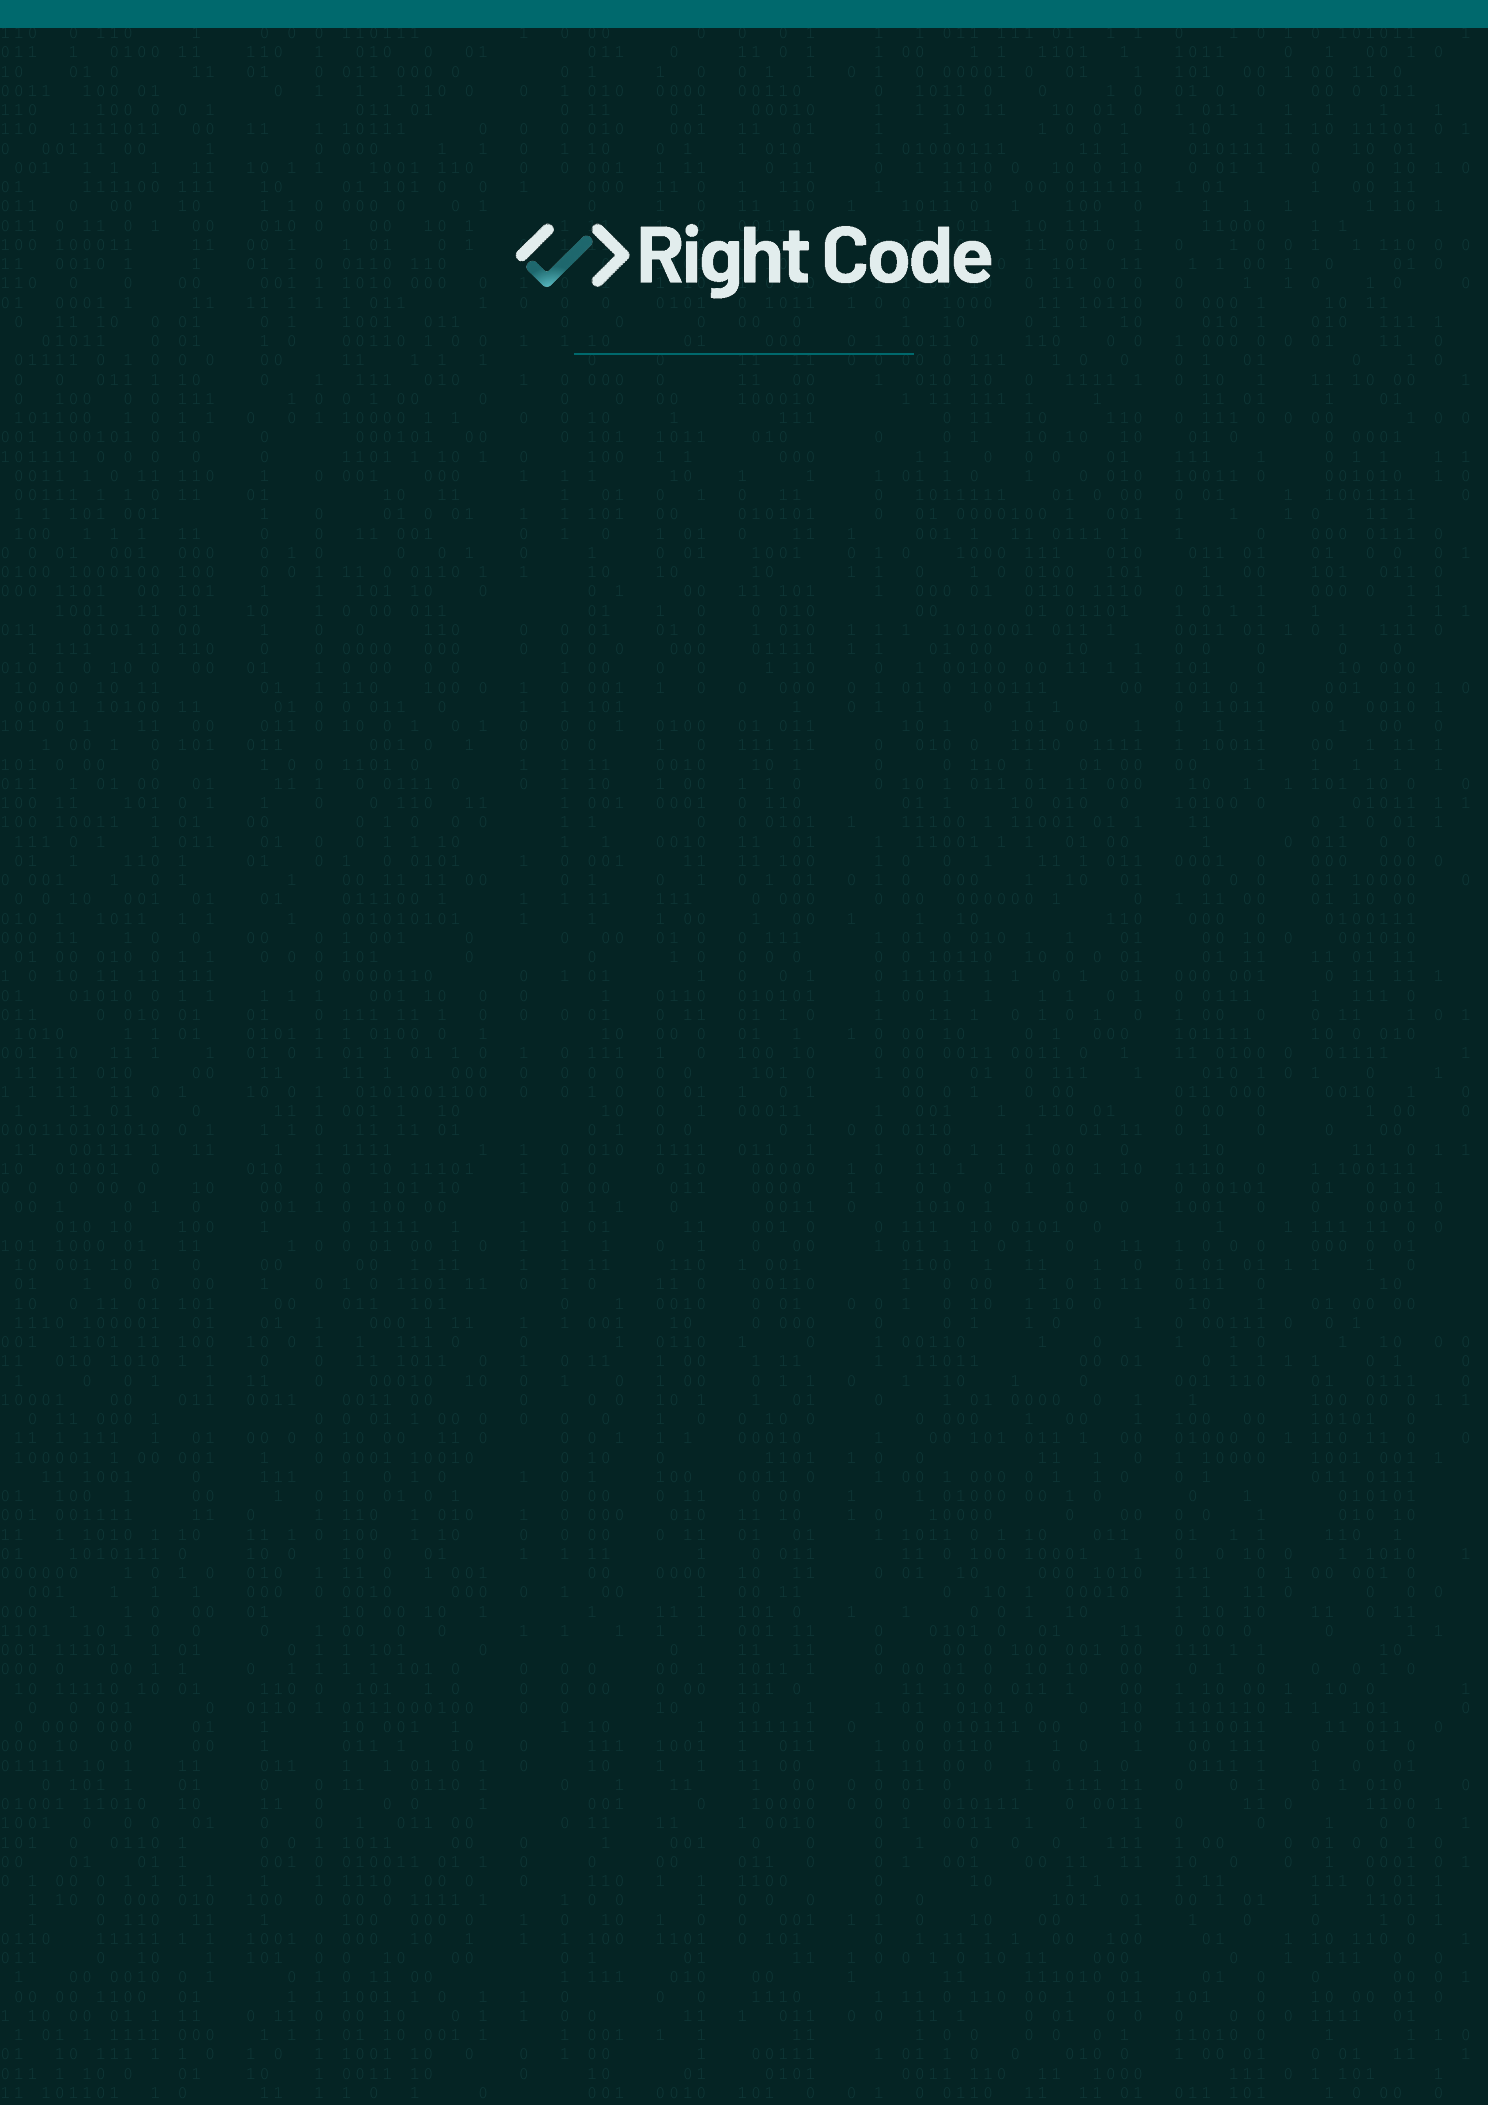
\includegraphics[width=\paperwidth,height=\paperheight]{assets/cover-bg.png}}}}}
  \centering
  % template: top margin 7.2cm + 2.1cm before the kicker (page top = 2.6cm)
  \vspace*{6.4cm}
  {\bfseries\small\color{rcPrimaryLight}#1\par}
  \vspace{14pt}
  {\bfseries\fontsize{22}{36}\selectfont\color{white}#2\par}
  \vspace{8pt}
  {\bfseries\small\color{rcPrimaryLight}#3\par}
  \vspace{5.2cm}
  % Meta strip: 3 equal cells, label above value (template cover table).
  % Drawn with TikZ: table cells reset the text color under bidi.
  \begin{tikzpicture}[x=4.6cm]
    \foreach \i/\lbl/\val in {0/التاريخ/{#4},-1/الإصدار/{#5},-2/أُعدّ بواسطة/{#6}}{
      \node[font=\bfseries\fontsize{7.5}{10}\selectfont,text=rcMutedDark] at (\i,0.5) {\RL{\lbl}};
      \node[font=\fontsize{9.5}{12}\selectfont,text=rcSurfaceVar] at (\i,0) {\RL{\val}};
    }
  \end{tikzpicture}
  \vfill
  \end{titlepage}
  \pagenumbering{arabic}%
  \rcwatermarktrue}

% ---------- Tables (RightCode brand table style) ----------
% Teal header band, white bold labels, zebra rows, hairline borders.
\newcolumntype{R}[1]{>{\raggedleft\arraybackslash}p{#1}}
\newcolumntype{Y}{>{\raggedleft\arraybackslash}X}
\newcommand{\rcHeaderRow}{\rowcolor{rcPrimary}}
\newcommand{\thh}[1]{\textcolor{white}{\bfseries #1}}
\newcommand{\rcZebra}{\rowcolors{2}{white}{rcSurfaceElev}}
\arrayrulecolor{rcBorder}
\setlength{\arrayrulewidth}{0.4pt}
\renewcommand{\arraystretch}{1.35}

% Data-classification badges (used in every "Before you start" table)
\newcommand{\rcbadge}[2]{\tikz[baseline=(b.base)]\node[fill=#1,text=white,
  rounded corners=2pt,inner xsep=4pt,inner ysep=1.5pt,font=\scriptsize\bfseries](b){\RL{#2}};}
\newcommand{\req}{\rcbadge{rcPrimary}{إلزامي تقنياً}}
\newcommand{\rec}{\rcbadge{rcPrimaryLight}{موصى به}}
\newcommand{\opt}{\rcbadge{rcMuted}{اختياري}}
\newcommand{\gen}{\rcbadge{rcTextSecondary}{يولّده النظام}}

% ---------- Image explanation (printed directly under a figure) ----------
\newcommand{\shotnote}[1]{\par\vspace{2pt}{\small #1\par}}

% ---------- Checklists ----------
\newlist{checklist}{itemize}{2}
\newcommand{\rccheckbox}{\tikz[baseline=-0.25ex]\draw[rcPrimary,line width=0.9pt,
  rounded corners=1pt](0,-0.05)rectangle(0.3,0.25);}
\setlist[checklist]{label={\rccheckbox},
  leftmargin=*,itemsep=2pt,topsep=4pt}
\newtcolorbox{rcchecklist}[1][قائمة تحقق]{enhanced,breakable,
  colback=rcSurfaceElev,colframe=rcPrimary,boxrule=0pt,
  leftrule=0pt,rightrule=3pt,arc=2pt,
  fonttitle=\bfseries\color{rcPrimary},coltitle=rcPrimary,
  colbacktitle=rcSurfaceElev,title={#1},
  left=10pt,right=10pt,top=4pt,bottom=6pt}

% ---------- Callouts ----------
\newtcolorbox{rcnote}[1][ملاحظة]{enhanced,breakable,colback=rcInfoBg,
  colframe=rcInfo,boxrule=0pt,rightrule=3pt,arc=2pt,
  title={#1},fonttitle=\bfseries,coltitle=rcInfo,colbacktitle=rcInfoBg}
\newtcolorbox{rcwarn}[1][تنبيه]{enhanced,breakable,colback=rcWarningBg,
  colframe=rcWarning,boxrule=0pt,rightrule=3pt,arc=2pt,
  title={#1},fonttitle=\bfseries,coltitle=rcWarning,colbacktitle=rcWarningBg}

% ---------- Diagram conventions (fixed for the whole guide) ----------
% RULE: TikZ nodes are laid out left-to-right. Wrap every Arabic label in
% \RL{...} (one \RL per line in multi-line nodes), e.g. \node[entity]{\RL{المناصب}};
% Boxes:   solid teal = required entity/page, dashed = optional,
%          grey fill  = generated by the system.
% Arrows:  solid  "dependsOn"  A -> B  means "A requires B to exist first".
%          dashed "flowsTo"    A -> B  means "the process moves from A to B".
\tikzset{
  rc/.style={font=\small,align=center},
  entity/.style={rc,draw=rcPrimary,line width=0.9pt,fill=white,
    rounded corners=3pt,minimum width=2.6cm,minimum height=0.95cm},
  entityOpt/.style={entity,dashed,draw=rcPrimaryLight},
  entityGen/.style={entity,draw=rcMuted,fill=rcSurfaceElev,text=rcTextSecondary},
  stepBox/.style={rc,fill=rcPrimary,text=white,rounded corners=3pt,
    minimum width=2.6cm,minimum height=0.95cm,font=\small\bfseries},
  dependsOn/.style={-{Stealth[length=7pt]},line width=1pt,draw=rcPrimary},
  dependsOnOpt/.style={dependsOn,densely dotted,draw=rcPrimaryLight},
  flowsTo/.style={-{Latex[length=6pt,open]},line width=1pt,draw=rcTextSecondary,
    densely dashed},
  edgeLabel/.style={font=\scriptsize,fill=white,inner sep=1.5pt,text=rcTextSecondary},
}
% Legend placed under each diagram
% Inline "depends on" arrow for running text: \dep  (e.g. التعيينات \dep{} الأعضاء)
\newcommand{\dep}{\,\tikz[baseline=-0.6ex]\draw[dependsOn](0.55,0)--(0,0);\,}
% Legend: items run right-to-left; each = symbol, then its label.
\newcommand{\rclegendItem}[3]{% #1 previous anchor, #2 symbol code, #3 label
  #2 \node[anchor=east,inner xsep=3pt] (lg) at (lgsym.west) {\RL{#3}};}
\newcommand{\rclegend}{%
  \par\smallskip
  \begin{tikzpicture}[font=\footnotesize,text=rcTextSecondary]
    \draw[dependsOn] (0,0.15) -- (0,-0.2);
    \node[anchor=east] at (-0.25,0) {\RL{متصل: يحتاج السجل المشار إليه أولاً}};
    \draw[dependsOnOpt] (0,-0.4) -- (0,-0.75);
    \node[anchor=east] at (-0.25,-0.55) {\RL{منقّط: ارتباط اختياري؛ الإطار المتقطع اختياري أيضاً}};
    \draw[flowsTo] (0,-0.95) -- (0,-1.3);
    \node[anchor=east] at (-0.25,-1.1) {\RL{متقطع برأس مفتوح: ثم انتقل إلى الخطوة التالية}};
  \end{tikzpicture}\par}

% ---------- Lists ----------
\setlist[itemize]{label={\color{rcPrimary}\textbullet},leftmargin=*,itemsep=1pt}
% Numbered lists: bold teal number, no dot (a trailing dot flips side in RTL)
\setlist[enumerate]{label={\textcolor{rcPrimary}{\bfseries\en{\arabic*}}},
  leftmargin=*,itemsep=2pt}

% ---------- Numbering: keep "1.2" left-to-right with a dot ----------
% (polyglossia's Arabic numbering reverses the parts and uses a comma)
% Digits in the Arabic font are shaped right-to-left, so numbers use Lora.
\newcommand{\rcnum}[1]{\LR{\textenglish{#1}}}
\AtBeginDocument{%
  \renewcommand{\thesection}{\rcnum{\thechapter.\arabic{section}}}%
  \renewcommand{\thesubsection}{\rcnum{\thechapter.\arabic{section}.\arabic{subsection}}}%
  \renewcommand{\thetable}{\rcnum{\thechapter.\arabic{table}}}%
  \renewcommand{\thefigure}{\rcnum{\thechapter.\arabic{figure}}}%
}

% Appendices: "الملحق أ", sections numbered 1, 2… (Latin letters would mix scripts)
\AtBeginDocument{%
  \gappto\appendix{%
    \gappto\captionsarabic{\renewcommand{\appendixname}{الملحق}}%
    \renewcommand{\appendixname}{الملحق}%
    \renewcommand{\thechapter}{\ifcase\value{chapter}\or أ\or ب\or ج\or د\or هـ\fi}%
    \renewcommand{\thesection}{\rcnum{\arabic{section}}}%
    \renewcommand{\thetable}{\rcnum{\arabic{table}}}%
    \renewcommand{\thefigure}{\rcnum{\arabic{figure}}}}%
}

\pagestyle{rcbody}


\begin{document}

\makecover{\en{KayanOS} · دليل المستخدم}
  {دليل نظام \kos}
  {من فهم احتياجات العمل إلى التطبيق خطوة بخطوة}
  {تشرين الأول 2026}{\en{0.3} — مسودة}{\en{RightCode}}

\tableofcontents

% ---- الفصول (بترتيب رحلة التأسيس) ----
% الفصل 1 — تعرّف إلى كيان من واقع عملك. قيد المراجعة.
\chapter{تعرّف إلى كيان: من تشتّت العمل إلى وضوحه}
\label{ch:intro}

\section{ما هو كيان، ولماذا قد تحتاجه؟}
\label{sec:intro-minute}
تخيّل أن أسماء الموظفين في ملف، وطلبات العمل في المحادثات، ومواعيد التسليم في
دفتر المدير. عندما يسأل عميل عن طلبه، تحتاج إلى سؤال عدة أشخاص لتعرف من يتابعه
وأين توقف. ومع توسّع الفريق يصبح هذا البحث جزءاً من العمل اليومي.

\textbf{كيان}، \kos، مساحة عمل تجمع إدارة الموظفين والمهام
والمشاريع والطلبات والملفات. يساعد فريقك على تسجيل العمل، وتحديد المسؤول عنه،
ومتابعة حالته، والرجوع إلى معلوماته وفق صلاحيات كل شخص.

\begin{table}[H]
\centering
\caption{من مشكلة يومية إلى استخدام واضح}
\label{tab:intro-minute}
\rcZebra
\begin{tabularx}{\linewidth}{Y Y Y}
\rcHeaderRow
\thh{المشكلة في العمل} & \thh{ما يقدمه كيان} & \thh{الفائدة العملية}\\
لا نعرف من يتابع العمل أو موعده. & مهام لها مسؤول وموعد وحالة. & تفتح المهمة لتعرف من يعمل عليها وما بقي.\\
بيانات الموظف ووظيفته موزعة. & أعضاء ومناصب وتعيينات في الموارد البشرية. & تعرف من يشغل كل وظيفة وأين يعمل.\\
الطلبات تصل بطرق مختلفة وتنقصها معلومات. & نماذج وطلبات ومسارات مراجعة تُعدّ حسب العمل. & تجمع المعلومات المطلوبة وتتابع الطلب في مكان معروف.\\
يصعب العثور على مستند العمل. & مكتبة ملفات ومرفقات مرتبطة بالعمل. & يرجع الفريق إلى المستند الذي يحتاجه.\\
المدير يحتاج صورة عن سير العمل. & حالات ومشاريع ولوحات معلومات عند إعدادها. & يراجع العمل المسجل ويحدد ما يحتاج متابعة.\\
\end{tabularx}
\end{table}

\textbf{ما تحتاجه المؤسسة لنجاح الاستخدام:} تحدد المسؤوليات، وتدخل بيانات صحيحة،
وتتفق على معنى «مكتمل». يتيح كيان تنظيم هذه الأمور، ويحدّث الفريق المعلومات أثناء
العمل حتى تكون المتابعة مفيدة.

\clearpage
\section{مثال بسيط: يوم عمل في شركة الأفق}
\label{sec:intro-entity}
نستخدم طوال الدليل شركة وهمية اسمها \textbf{شركة الأفق للخدمات}، لها مقر في دمشق
وفرع في حلب. سارة تدير الموارد البشرية، وعمر منسق عمليات في فرع حلب.

يصل طلب تجهيز مكتب لموظف جديد. \textbf{قبل تنظيم العمل}، قد يبقى الطلب في
محادثة، ويسأل المدير أكثر من مرة: من يجهز المكتب؟ ومتى ينتهي؟ وأين فاتورة الشراء؟

\textbf{باستخدام كيان} يمكن للفريق العمل بهذه الصورة، بعد إعداد الأدوات المناسبة:
\begin{enumerate}
  \item يسجل الطلب ومعلوماته، فيصبح له مكان يرجع إليه الجميع المخوّلون.
  \item يحدد المدير العمل المطلوب من عمر وموعده في مهمة واضحة.
  \item يحدّث عمر حالة المهمة ويضيف النتيجة أو المستند المطلوب.
  \item يفتح المدير العمل ليراجع النتيجة ويتابع ما لم ينتهِ بعد.
\end{enumerate}
هذا مثال لطريقة تنظيم العمل. إنشاء الطلب لا يولّد بقية الخطوات تلقائياً؛
أي انتقال تلقائي يحتاج إلى إعداد مسبق يناسب المؤسسة.

\section{ما الذي ستستخدمه أنت؟}
\begin{table}[H]
\centering
\caption{ابدأ بحسب مسؤوليتك}
\label{tab:intro-roles}
\rcZebra
\begin{tabularx}{\linewidth}{R{3.4cm} Y Y}
\rcHeaderRow
\thh{دورك في العمل} & \thh{ما تريد إنجازه} & \thh{من أين تبدأ؟}\\
صاحب العمل أو المدير & فهم ما يقدمه النظام واختيار أول عمل لتنظيمه. & هذا الفصل، ثم مثال صغير في قسم واحد.\\
مسؤول إعداد النظام & تجهيز المؤسسة وحسابات الفريق والأقسام. & الفصل~\ref{ch:org-setup}.\\
مسؤول الموارد البشرية & تنظيم الموظفين والدوام والإجازات والرواتب. & الفصل~\ref{ch:hr} بعد تجهيز الفريق.\\
الموظف & الوصول إلى عمله ومتابعته. & خطوات الدخول التالية؛ لا يحتاج إلى إنشاء مؤسسة جديدة.\\
\end{tabularx}
\end{table}

\textbf{اختر بداية صغيرة:} في شركة الأفق نبدأ بموظفين ووظيفتين وجدول دوام واحد.
نتأكد من النتيجة، ثم نضيف بقية الفريق. لا يلزم تشغيل كل التطبيقات في اليوم الأول.

\clearpage
\section{أول دخول: أين تجد عملك؟}
\label{sec:intro-app-map}
\textbf{قبل البدء:} اطلب من مسؤول مؤسستك عنوانها وطريقة دخولك. العنوان مثل
\en{hzn.kayanos.app} في مثالنا؛ استخدم عنوان مؤسستك الحقيقي. إذا كنت تؤسس
المؤسسة لأول مرة، انتقل إلى الفصل~\ref{ch:org-setup}.

\begin{enumerate}
  \item افتح عنوان المؤسسة في المتصفح. اختر طريقة الدخول التي جهّزها لك المسؤول:
        البريد الإلكتروني، أو الهاتف، أو رقم الموظف، ثم أدخل بيانات دخولك.
  \item بعد الدخول، تأكد أنك في المؤسسة المقصودة قبل إدخال أي بيانات.
  \item افتح «مشغّل التطبيقات» من الصفحة الرئيسية، واختر «الموارد البشرية» كمثال.
  \item افتح «القوى العاملة»، ثم «الأعضاء». هذه قائمة الموظفين، وليست صفحة موظف واحد.
  \item افتح اسم موظف لعرض تفاصيله. للرجوع اختر اسم الصفحة أو التطبيق من مسار
        التنقل أعلى الشاشة. ويمكن استخدام البحث للعثور على عمل أو شخص متاح لك.
\end{enumerate}

\begin{figure}[H]
\centering
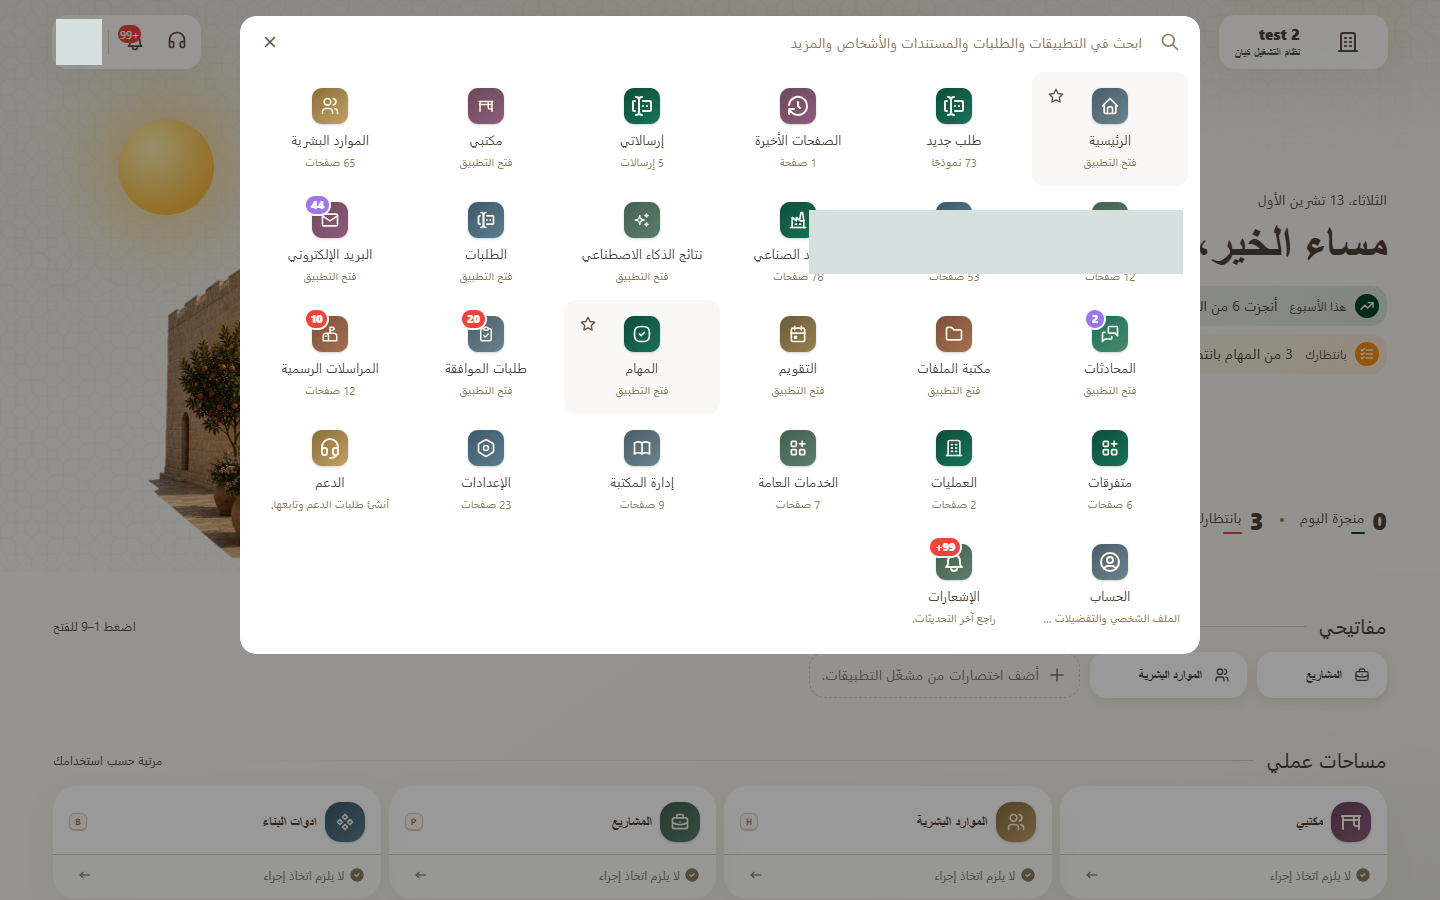
\includegraphics[width=0.7\linewidth]{figures/screens/ch01-apps-directory.png}
\caption{اختر التطبيق الذي يخدم عملك من مشغّل التطبيقات}
\label{fig:intro-apps-directory}
\end{figure}



\clearpage
\section{افهم أسماء الشاشة من مثال واحد}
\label{sec:intro-concepts}
نريد أن يعرف النظام أن سارة تعمل مديراً للموارد البشرية في دمشق.
هذه هي الأسماء التي ستقابلها، ومعنى كل اسم في هذا المثال:

\begin{table}[H]
\centering
\caption{لغة العمل وأسماؤها في كيان}
\label{tab:intro-terms}
\rcZebra
\begin{tabularx}{\linewidth}{R{3.4cm} Y}
\rcHeaderRow
\thh{اسم الشاشة} & \thh{معناه ببساطة}\\
المؤسسة & مساحة عمل شركة الأفق وحسابات فريقها.\\
العضو & الشخص الذي يعمل معنا: سارة الخطيب.\\
الوحدة التنظيمية & القسم أو الإدارة: الموارد البشرية.\\
النقطة الجغرافية & مكان العمل: المقر الرئيسي في دمشق.\\
المنصب & الوظيفة: مدير الموارد البشرية.\\
التعيين & تحديد أن سارة هي من تشغل هذه الوظيفة خلال فترة عملها.\\
الدور والصلاحيات & ما يُسمح لسارة أن تراه أو تفعله، مثل عرض الموظفين أو تعديل بياناتهم.\\
\end{tabularx}
\end{table}

\begin{figure}[H]
\centering
\begin{tikzpicture}[node distance=0.65cm]
  \node[entity] (asg) {\RL{تعيين سارة في وظيفتها}};
  \node[entity,below right=0.7cm and 0.4cm of asg] (mem) {\RL{سارة الخطيب}\\\RL{العضو}};
  \node[entity,below left=0.7cm and 0.4cm of asg] (pos) {\RL{مدير الموارد البشرية}\\\RL{المنصب}};
  \node[entityOpt,below=of pos] (node) {\RL{قسم الموارد البشرية}};
  \draw[dependsOn] (asg.south) -- ++(0,-0.3) -| (mem.north);
  \draw[dependsOn] (asg.south) -- ++(0,-0.3) -| (pos.north);
  \draw[dependsOnOpt] (pos.south) -- (node.north);
\end{tikzpicture}
\rclegend
\caption{أنشئ بيانات الشخص والوظيفة، ثم اربطهما بتعيين}
\label{fig:intro-structure}
\end{figure}
التعيين يحتاج إلى شخص ووظيفة موجودين.
ربط الوظيفة بقسمها اختياري تقنياً، لكنه يساعدك على معرفة موظفي كل قسم.

\clearpage
\section{ما الذي تختاره لكل نوع من العمل؟}
\begin{table}[H]
\centering
\caption{اختر التطبيق بناءً على ما تريد إنجازه}
\label{tab:intro-app-map}
\rcZebra
\begin{tabularx}{\linewidth}{Y Y}
\rcHeaderRow
\thh{أريد أن...} & \thh{أبدأ من...}\\
أعرف الموظفين ووظائفهم وأراجع دوامهم. & الموارد البشرية.\\
أسند عملاً لشخص وأتابع تنفيذه. & المهام.\\
أنظم عملاً أكبر له خطة وأعمال مترابطة. & المشاريع.\\
أقدم طلباً أو أراجع طلباً ينتظر قراري. & الطلبات أو الموافقات المتاحة في المؤسسة.\\
أرتب موعداً أو أرجع إلى ملف أو محادثة. & التقويم أو مكتبة الملفات أو أدوات التواصل.\\
أجهز نموذجاً خاصاً بعمل المؤسسة. & أدوات البناء، ويتولاها المسؤول المخوّل.\\
\end{tabularx}
\end{table}

\section{كيف تنتقل من الفهم إلى التشغيل؟}
\label{sec:intro-how-to-read}
الفصل التالي يقود مسؤول الإعداد إلى تسجيل فريق صغير. ثم يشرح فصل الموارد البشرية
كيفية تحديد دوامه ومراجعته. أما فصول المهام والمشاريع فستُضاف لاحقاً إلى هذا الدليل.

\begin{figure}[H]
\centering
\begin{tikzpicture}[node distance=0.4cm,stepBox/.append style={minimum width=6cm,text width=5.6cm,minimum height=0.7cm,font=\small\bfseries}]
  \node[stepBox] (s1) {\RL{اختر عملاً تريد تنظيمه}};
  \node[stepBox,below=of s1] (s2) {\RL{جهّز المؤسسة والفريق}};
  \node[stepBox,below=of s2] (s3) {\RL{طبّق مثالاً صغيراً}};
  \node[stepBox,below=of s3] (s4) {\RL{تحقّق من النتيجة مع المستخدم}};
  \node[stepBox,below=of s4] (s5) {\RL{وسّع الاستخدام إلى بقية الفريق}};
  \foreach \a/\b in {s1/s2,s2/s3,s3/s4,s4/s5} \draw[flowsTo] (\a) -- (\b);
\end{tikzpicture}
\rclegend
\caption{ابدأ بنتيجة صغيرة مفيدة، ثم وسّع الاستخدام}
\label{fig:intro-journey}
\end{figure}

\textbf{علامات تساعدك أثناء التطبيق:} \req{} مطلوب للحفظ، \rec{} يساعدك على
تنظيم العمل، \opt{} تستخدمه عند الحاجة، \gen{} يملؤه النظام. أمثلة الأفق للتعلّم؛
استبدلها ببيانات مؤسستك عند التطبيق الفعلي.

% =====================================================================
%  الفصل 2 — إنشاء المؤسسة والتهيئة الأولية
%  الحالة: قيد المراجعة
% =====================================================================
\chapter{إنشاء المؤسسة والتهيئة الأولية}
\label{ch:org-setup}

\section{جهّز مكاناً واحداً لبيانات فريقك}
\label{sec:setup-minute}

عندما يُكتب اسم الموظف وقسمه في أكثر من ملف، يصعب الحفاظ على نسخة صحيحة.
سنجهّز في كيان تعريفاً واضحاً للفريق: من يعمل معنا، وفي أي وظيفة وقسم وموقع.
تستخدم التطبيقات هذه البيانات لاحقاً بدلاً من إعادة إدخالها في كل مرة.

\textbf{من ينفذ؟} مسؤول إعداد النظام، بالتعاون مع المسؤول عن الموظفين.

\textbf{متى؟} عند بدء استخدام المؤسسة.

\textbf{نتيجة التمرين:} تستطيع فتح تعيين سارة، ورؤية وظيفتها وقسمها وموقع عملها.
سنبدأ بسارة، ثم تكرر الخطوات لعمر وبقية الفريق.

\begin{figure}[H]
\centering
\begin{tikzpicture}[node distance=0.45cm,stepBox/.append style={minimum width=5cm,text width=4.6cm,minimum height=0.7cm,font=\small\bfseries}]
  \node[stepBox]            (s1) {\RL{إنشاء}\\\RL{المؤسسة}};
  \node[stepBox,below=of s1] (s2) {\RL{إعدادات المؤسسة}};
  \node[stepBox,below=of s2] (s3) {\RL{المواقع والوحدات}};
  \node[stepBox,below=of s3] (s4) {\RL{المناصب}};
  \node[stepBox,below=of s4] (s5) {\RL{الأعضاء}};
  \node[stepBox,below=of s5] (s6) {\RL{التعيينات}};
  \foreach \a/\b in {s1/s2,s2/s3,s3/s4,s4/s5,s5/s6} \draw[flowsTo] (\a) -- (\b);
\end{tikzpicture}
\rclegend
\caption{خطوات الفصل الست}
\label{fig:setup-steps}
\end{figure}

\section{قبل أن تبدأ}
\label{sec:setup-before}

جهّز قائمة صغيرة من أسماء الأقسام والمواقع والوظائف والموظفين، وحدد من يراجعها.
\textbf{الرمز} هو معرّف تختاره لتجنب الخلط بين الأسماء، مثل \en{HZN-HR} لقسم
الموارد البشرية؛ لا يحتاج إلى معرفة برمجية. \textbf{النطاق الفرعي} هو الجزء الذي
تختاره لعنوان مؤسستك، مثل \en{hzn} في \en{hzn.kayanos.app}.

\begin{table}[H]
\centering
\caption{ما تحتاج تجهيزه قبل الإنشاء}
\label{tab:setup-before}
\rcZebra
\begin{tabularx}{\linewidth}{R{4cm} R{2.4cm} Y}
\rcHeaderRow
\thh{البيان} & \thh{التصنيف} & \thh{ملاحظة}\\
بريد إلكتروني أو رقم هاتف & \req & يصله رمز التحقق.\\
اسم المؤسسة & \req & يمكن كتابته بأكثر من لغة.\\
النطاق الفرعي & \req & عنوان المؤسسة، مثل \en{hzn}.\\
البلد وعدد الموظفين & \req & عدد الموظفين تقديري (فئة).\\
اسم المدير & \req & صاحب الحساب الأول.\\
كلمة مرور المدير & \opt & إن تُركت فارغة يصلك رمز لتعيينها لاحقاً.\\
الشعار & \opt & صورة حتى \en{5} ميغابايت.\\
\end{tabularx}
\end{table}

\section{الخطوة 1: إنشاء المؤسسة}
\label{sec:setup-create}

من شاشة الدخول افتح «إنشاء مؤسسة». هذه الخطوة لصاحب المؤسسة أو المسؤول الذي
يجهزها أول مرة، وليست لكل موظف جديد. اتبع الخطوات الأربع:

\begin{figure}[H]
\centering
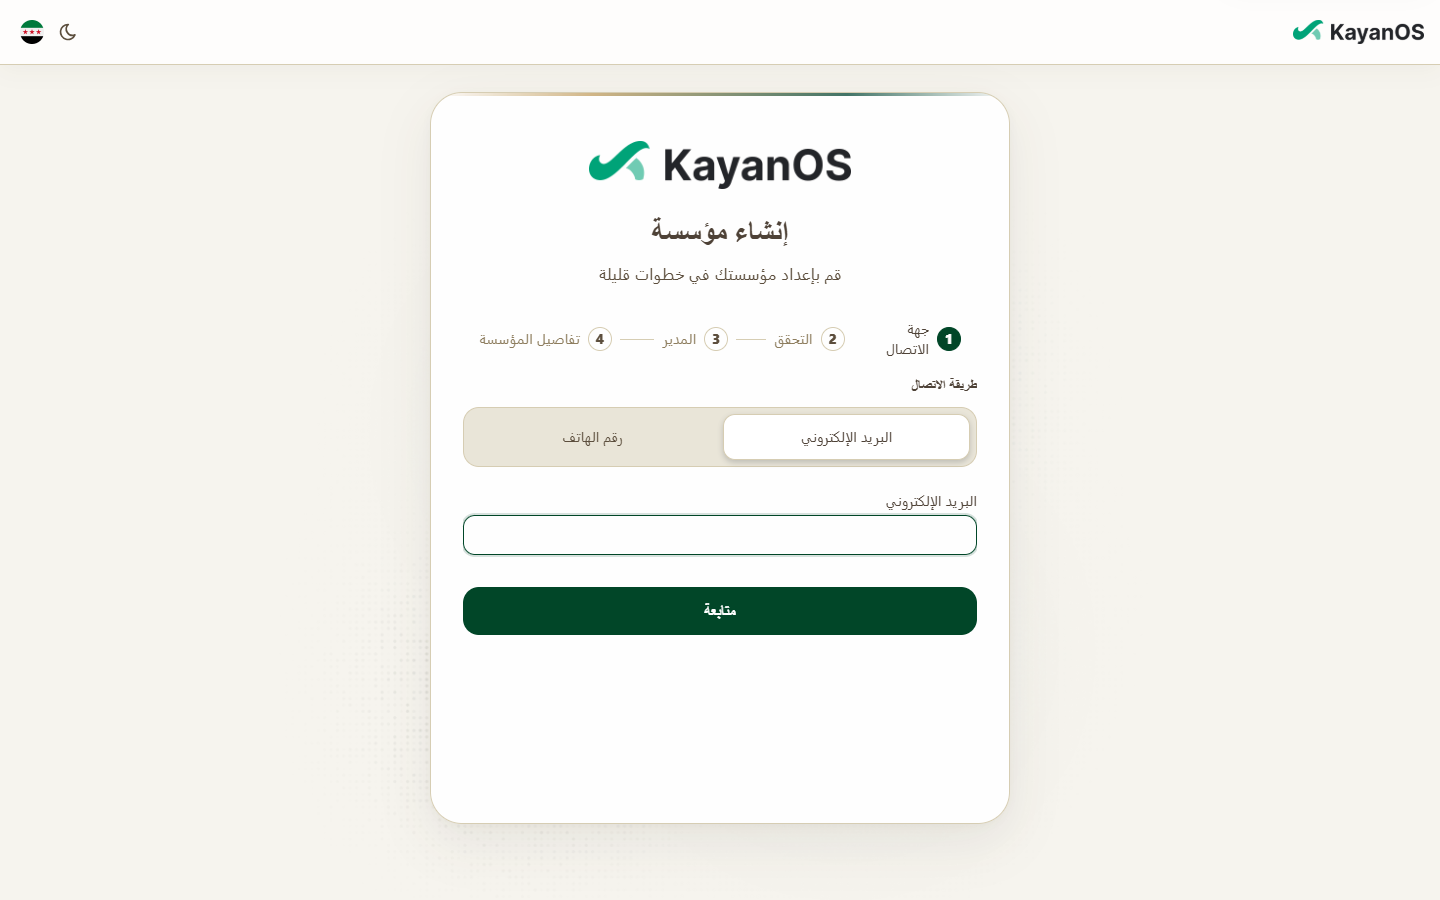
\includegraphics[width=0.62\linewidth]{figures/screens/ch02-create-org.png}
\caption{صفحة «إنشاء مؤسسة»: الخطوات الأربع في الأعلى}
\label{fig:setup-create-screen}
\end{figure}

\begin{enumerate}
  \item \textbf{جهة الاتصال:} اختر البريد الإلكتروني أو رقم الهاتف وأدخله.
  \item \textbf{التحقق:} أدخل الرمز المكوّن من \en{6} أرقام. الرمز صالح \en{10}
        دقائق، ويمكن طلب رمز جديد بعد دقيقة.
  \item \textbf{المدير:} اكتب اسمك، وكلمة مرور إن أردت.
  \item \textbf{تفاصيل المؤسسة:} النطاق الفرعي، والاسم، والبلد، وعدد الموظفين، والشعار.
\end{enumerate}

بعد إكمال الإنشاء تنتقل إلى عنوان مؤسستك الجديد لتسجيل الدخول.
\textbf{تحقّق:} افتح العنوان الجديد بحساب المسؤول، وتأكد من اسم المؤسسة.
احتفظ بالعنوان ليستخدمه فريقك؛ اسم المؤسسة وحده لا يكفي للوصول إليها.

\begin{rcnote}[شروط النطاق الفرعي]
من \en{3} إلى \en{63} حرفاً: أحرف إنجليزية صغيرة وأرقام وشرطة (-)، ولا يبدأ أو
ينتهي بشرطة. يجب أن يكون غير مستخدم، وبعض الكلمات محجوزة مثل \en{admin} و\en{www}.
\end{rcnote}

\subsection{ماذا ينشئ النظام تلقائياً؟}

\begin{table}[H]
\centering
\caption{ما تجده جاهزاً وما عليك إدخاله}
\label{tab:setup-generated}
\rcZebra
\begin{tabularx}{\linewidth}{Y Y}
\rcHeaderRow
\thh{جاهز بعد الإنشاء} & \thh{عليك إدخاله}\\
حسابك كعضو، مع دور «المدير». & النقاط الجغرافية (المواقع).\\
الأدوار الأساسية. & الوحدات التنظيمية.\\
التطبيقات وتعريفات الكيانات. & المناصب.\\
العملات وقوالب الحالات. & الأعضاء والتعيينات والورديات.\\
\end{tabularx}
\end{table}

\section{الخطوة 2: إعدادات المؤسسة}
\label{sec:setup-settings}

من مشغّل التطبيقات افتح \textbf{الإعدادات}، ثم \textbf{الإدارة}، ثم
\textbf{إعدادات المؤسسة}. الهدف أن يرى الفريق الأوقات واللغة المناسبة لعمله.

\begin{table}[H]
\centering
\caption{إعدادات تراجعها فوراً}
\label{tab:setup-settings}
\rcZebra
\begin{tabularx}{\linewidth}{R{4.2cm} R{2.6cm} Y}
\rcHeaderRow
\thh{الإعداد} & \thh{القيمة الافتراضية} & \thh{لماذا يهم؟}\\
المنطقة الزمنية الافتراضية & \en{UTC} & تحدد أوقات الدوام والمواعيد والتقارير.\\
اللغة الافتراضية & \en{English} & لغة الواجهة للأعضاء الجدد.\\
يوم بداية الأسبوع & الاثنين & يؤثر على التقويم والتقارير الأسبوعية.\\
الشعار واللون الأساسي & — & هوية المؤسسة في الواجهة (اختياري).\\
\end{tabularx}
\end{table}

في مثال الأفق اختر \en{Asia/Damascus} للمنطقة الزمنية، والعربية للغة الافتراضية،
ويوم بداية الأسبوع الذي تعتمده المؤسسة. احفظ التغييرات ثم افتح الإعدادات مرة أخرى
لتتأكد من بقاء القيم. راجع هذه الخيارات قبل إدخال الفريق أو متابعة الدوام.

\section{ترتيب البيانات الأساسية}
\label{sec:setup-order}

تجدها كلها في تطبيق \textbf{الموارد البشرية}. الترتيب مهم لأن بعضها يشير إلى بعض:

\begin{figure}[H]
\centering
\begin{tikzpicture}[node distance=0.7cm]
  \node[entity] (asg) {\RL{التعيينات}};
  \node[entity,below right=0.7cm and 0.5cm of asg] (mem) {\RL{الأعضاء}};
  \node[entity,below left=0.7cm and 0.5cm of asg] (pos) {\RL{المناصب}};
  \node[entityOpt,below right=0.7cm and 0.1cm of pos] (node) {\RL{الوحدات التنظيمية}};
  \node[entityOpt,below left=0.7cm and 0.1cm of pos] (loc) {\RL{النقاط الجغرافية}};
  \draw[dependsOn] (asg.south) -- ++(0,-0.3) -| (mem.north);
  \draw[dependsOn] (asg.south) -- ++(0,-0.3) -| (pos.north);
  \draw[dependsOnOpt] (pos.south) -- ++(0,-0.3) -| (node.north);
  \draw[dependsOnOpt] (pos.south) -- ++(0,-0.3) -| (loc.north);
\end{tikzpicture}
\rclegend
\caption{لماذا نجهّز بيانات الشخص والوظيفة قبل تعيينه؟}
\label{fig:setup-deps}
\end{figure}

ابدأ القراءة من «التعيينات» في أعلى الشجرة. السهم يبيّن السجل الذي يرتبط به ما فوقه؛
أما ترتيب الإدخال العملي فيبدأ بالسجلات المطلوبة قبل إنشاء التعيين.

\begin{itemize}
  \item \textbf{إلزامي:} لا يُحفظ التعيين إلا بعضو ومنصب موجودين.
  \item \textbf{اختياري لكن مُنصح به:} ربط المنصب بوحدته وموقعه. ابدأ بها حتى
        تختارها عند إنشاء المناصب.
  \item \textbf{التسلسل:} الوحدة الأم قبل الوحدات التابعة لها، وكذلك المواقع.
  \item \textbf{الورديات:} اختيارية هنا، ويشرحها القسم~\ref{sec:hr-shifts} من فصل الموارد البشرية.
\end{itemize}

\section{الخطوات 3 إلى 6: أضف أول موظف في وظيفته}
\label{sec:setup-data}

ابدأ بالإضافة اليدوية لتتعرف إلى الخطوات. \textbf{القائمة} تعرض الأشخاص أو الوظائف،
و\textbf{السجل} هو صفحة عنصر واحد منها، و\textbf{الحقل} هو خانة مثل الاسم.
عند اختيار قسم أو موظف من قائمة داخل النموذج، اختر العنصر الموجود بدلاً من
كتابة اسم جديد غير مرتبط به.

\subsection{جهّز مكان العمل والقسم}
\begin{enumerate}
  \item افتح «الموارد البشرية»، ثم «الأساسية»، ثم «النقاط الجغرافية»، واختر الإضافة.
        اكتب الرمز \en{HZN-DAM} والاسم «المقر الرئيسي، دمشق».
        اختر نوع الموقع المناسب من الخيارات المتاحة، ثم البلد والمحافظة والمدينة
        والعنوان الفعلي. احفظ، وارجع إلى القائمة لتتأكد من ظهور الموقع.
  \item افتح «الأساسية»، ثم «الوحدات التنظيمية»، وأضف «الإدارة العامة» برمز
        \en{HZN-GM} واحفظها. أضف بعدها «الموارد البشرية» برمز \en{HZN-HR}،
        واختر «الإدارة العامة» في حقل الوحدة الأم، ثم احفظ.
\end{enumerate}
\textbf{النتيجة:} القسم له مكان واضح في هيكل المؤسسة. إذا لم تظهر الوحدة الأم
في الاختيار، تأكد أنك حفظتها أولاً وأنك تعمل في المؤسسة نفسها.

\subsection{جهّز الوظيفة ثم الشخص ثم التعيين}
\begin{enumerate}
  \item افتح «القوى العاملة»، ثم «المناصب»، واختر الإضافة. أدخل
        \en{HZN-P-01} و«مدير الموارد البشرية»، واختر وحدة «الموارد البشرية»
        وموقع «المقر الرئيسي، دمشق»، ثم احفظ.
  \item افتح «القوى العاملة»، ثم «الأعضاء»، واختر الإضافة. أدخل رقم الموظف
        \en{0001} والاسم «سارة الخطيب». نوع المقعد يحدد فئة استخدام الحساب؛
        اختر «مقعد كامل» لهذا المثال، وأضف وسيلة التواصل الحقيقية عند إعداد موظف
        فعلي. احفظ وتأكد من ظهور سارة في القائمة.
  \item افتح «القوى العاملة»، ثم «التعيينات»، واختر الإضافة. اختر سارة في حقل
        «العضو»، و«مدير الموارد البشرية» في حقل «المنصب». أدخل تاريخ بدء العمل
        ونوع التوظيف المناسبين؛ في التدريب يمكن استخدام \en{2026-10-01} كتاريخ بدء.
        احفظ، ثم افتح التعيين مرة أخرى.
\end{enumerate}
\textbf{تحقّق:} يظهر في التعيين اسم سارة ومنصبها الصحيح. وجود سارة في قائمة
الأعضاء وحده لا يعني أنها عُيّنت في وظيفة. إذا لم تجدها في قائمة الاختيار، ابحث
برقم الموظف وتأكد من حفظ سجلها.

\begin{table}[H]
\centering
\caption{الحقول الإلزامية في كل خطوة}
\label{tab:setup-required}
\rcZebra
\begin{tabularx}{\linewidth}{R{3.3cm} R{4.8cm} Y}
\rcHeaderRow
\thh{الصفحة} & \thh{إلزامي} & \thh{مُنصح به}\\
النقاط الجغرافية & الرمز، الاسم، النوع، البلد، المحافظة، المدينة، العنوان & يتبع لـ (الموقع الأب)\\
الوحدات التنظيمية & الرمز & الاسم، الوحدة الأم\\
المناصب & الرمز، الاسم & الوحدة، الموقع\\
الأعضاء & رقم الموظف، الاسم، نوع المقعد & البريد الإلكتروني أو الهاتف\\
التعيينات & العضو، المنصب & نوع التوظيف، تاريخ البدء\\
\end{tabularx}
\end{table}

\begin{rcnote}[الرمز فريد]
لا تكرر الرمز داخل القائمة نفسها، ولا تغيّره عند تصحيح اسم سجل موجود.
للأعضاء استخدم رقم الموظف المتفق عليه. تسمية واضحة ورمز ثابت يساعدانك على اختيار
القسم أو الشخص الصحيح لاحقاً.
\end{rcnote}

\subsection{الاستيراد من Excel}
\label{sec:setup-import}

استخدم الاستيراد عندما تصبح لديك قائمة كبيرة وصحيحة. جرّب صفاً واحداً أولاً
وتحقق من النتيجة، ثم أكمل بقية الملف. هذا بديل للإدخال اليدوي، وليس خطوة إضافية
مطلوبة بعد إدخال الموظفين.

\begin{enumerate}
  \item افتح صفحة الكيان، مثل «المناصب»، واختر الاستيراد ثم نزّل القالب.
  \item الأعمدة المعلّمة بـ \textbf{*} إلزامية.
  \item اترك فارغةً الأعمدة التي يملؤها النظام: «المعرف» و«التسمية» وكل عمود يبدأ
        بكلمة «النشطة/النشطون»، مثل «المناصب النشطة».
  \item في أعمدة الربط، مثل «المنصب» أو «الوحدة»، اكتب \textbf{التسمية} كما تظهر
        في النظام تماماً.
  \item راجع المعاينة قبل التأكيد.
\end{enumerate}

\begin{figure}[H]
\centering
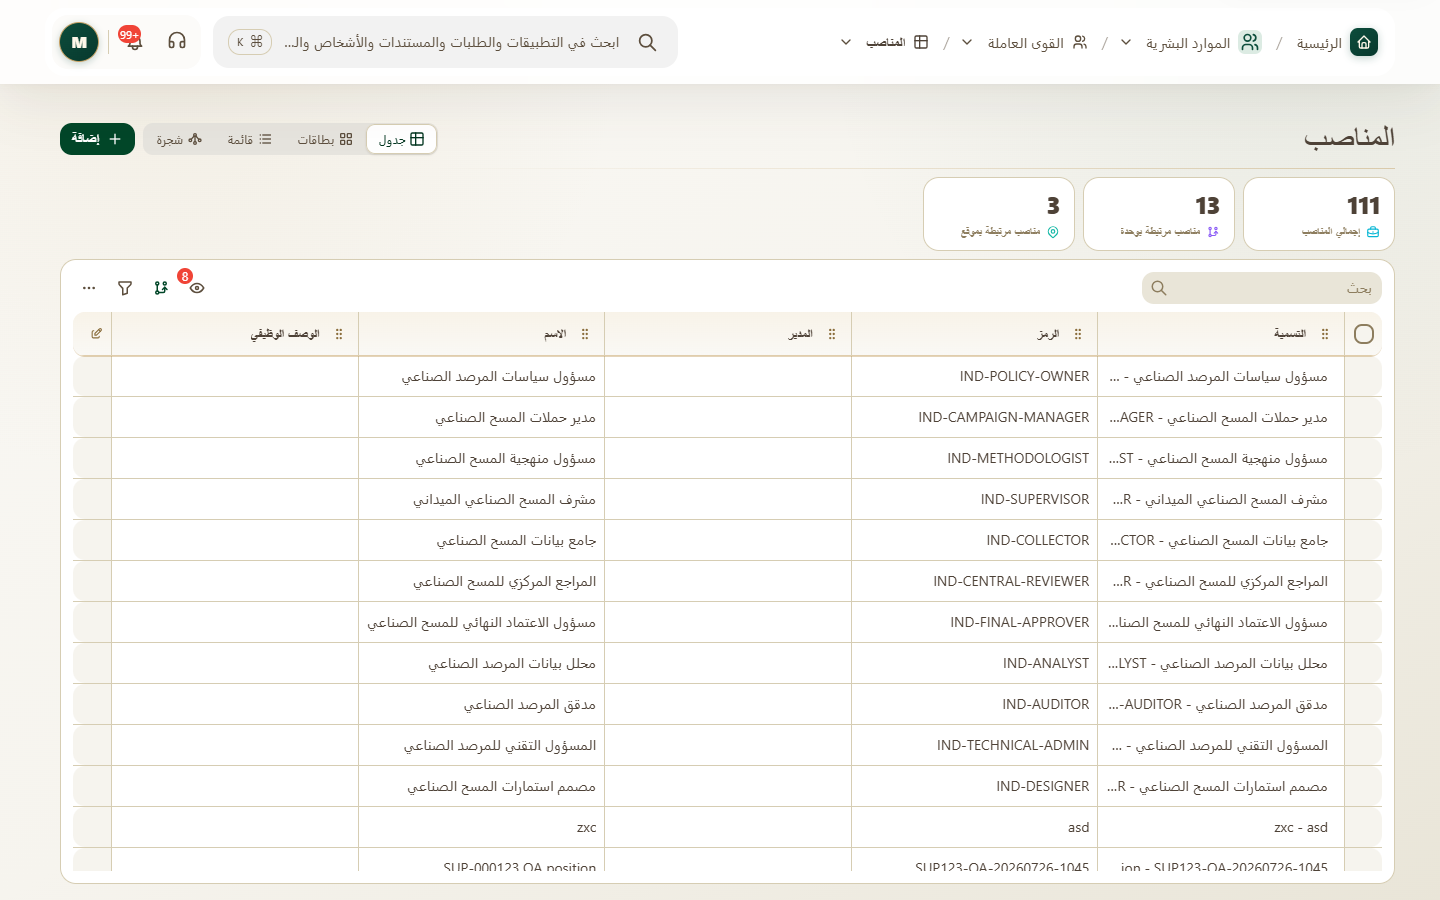
\includegraphics[width=0.9\linewidth]{figures/screens/ch02-positions.png}
\caption{صفحة المناصب: عمود «التسمية» يجمع الاسم والرمز. انسخه كما هو في أعمدة الربط}
\label{fig:setup-positions}
\end{figure}

\begin{rcwarn}[التحديث بدل التكرار]
إذا استوردت ملفاً فيه رمز موجود مسبقاً، \textbf{يُحدَّث} السجل الموجود ولا يُنشأ
سجل جديد. لتصحيح بيانات، عدّل الملف نفسه وأعد استيراده بالرموز نفسها. الصفوف المكررة
داخل الملف الواحد تُتجاهل.
\end{rcwarn}

\subsection{دخول الأعضاء إلى النظام}
\label{sec:setup-login}

بعد تجهيز الموظف، يحتاج إلى طريقة دخول. مسؤول النظام يجهزها، والموظف يختبرها
على عنوان المؤسسة. لا تعتبر ظهور اسمه في القائمة دليلاً على أنه دخل بنجاح.

\begin{itemize}
  \item \textbf{للعضو بريد أو هاتف:} ينشئ النظام دعوة بالبريد أو واتساب، صالحة
        \en{48} ساعة. يفتح الرابط ويختار كلمة مرور من \en{8} أحرف على الأقل.
  \item \textbf{ليس له بريد ولا هاتف:} يعيّن له المدير كلمة مرور، ويدخل برقم الموظف.
\end{itemize}

اطلب من الموظف فتح عنوان المؤسسة والدخول بالطريقة المحددة له، ثم فتح تطبيق
مسموح له. إذا لم تصل الدعوة، راجع صحة وسيلة التواصل مع المسؤول؛ وصول الرسالة
يعتمد أيضاً على قناة الإرسال، وليس مجرد وجود البريد أو الهاتف.

\section{مثال عملي: شركة الأفق للخدمات}
\label{sec:setup-example}

\begin{table}[H]
\centering
\caption{بيانات المثال بالترتيب}
\label{tab:setup-example}
\rcZebra
\begin{tabularx}{\linewidth}{R{3cm} R{2.6cm} Y}
\rcHeaderRow
\thh{الكيان} & \thh{الرمز} & \thh{البيانات}\\
نقطة جغرافية & \en{HZN-DAM} & المقر الرئيسي، دمشق\\
نقطة جغرافية & \en{HZN-ALP} & فرع حلب\\
وحدة & \en{HZN-GM} & الإدارة العامة\\
وحدة & \en{HZN-HR} & الموارد البشرية، تتبع الإدارة العامة\\
منصب & \en{HZN-P-01} & مدير الموارد البشرية، وحدة \en{HZN-HR}، موقع \en{HZN-DAM}\\
منصب & \en{HZN-P-02} & منسق عمليات، موقع \en{HZN-ALP}\\
عضو & \en{0001} & سارة الخطيب، مقعد كامل\\
عضو & \en{0002} & عمر حداد، مقعد كامل\\
تعيين & — & سارة \dep{} مدير الموارد البشرية\\
تعيين & — & عمر \dep{} منسق عمليات\\
\end{tabularx}
\end{table}

\section{تحقّق من النتيجة}
\label{sec:setup-check}

\begin{rcchecklist}[قائمة تحقق: اكتمال التهيئة]
\begin{checklist}
  \item المنطقة الزمنية واللغة الافتراضية مضبوطتان.
  \item كل وحدة تتبع وحدتها الأم الصحيحة.
  \item كل منصب مرتبط بوحدته وموقعه.
  \item كل عضو له تعيين واحد على الأقل.
  \item يظهر لكل منصب «الأعضاء النشطون» الذين يشغلونه.
  \item عضو تجريبي استلم الدعوة ودخل بنجاح.
\end{checklist}
\end{rcchecklist}

\section{أخطاء شائعة}
\label{sec:setup-errors}

\begin{table}[H]
\centering
\caption{أخطاء شائعة وحلولها}
\label{tab:setup-errors}
\rcZebra
\begin{tabularx}{\linewidth}{R{4.2cm} Y Y}
\rcHeaderRow
\thh{المشكلة} & \thh{السبب} & \thh{الحل}\\
النطاق الفرعي مرفوض & مستخدم، أو محجوز، أو فيه أحرف غير مسموحة. & اختر اسماً آخر بأحرف صغيرة وأرقام.\\
انتهت صلاحية رمز التحقق & مرّت \en{10} دقائق. & اطلب رمزاً جديداً.\\
فشل استيراد التعيينات & العضو أو المنصب غير موجود، أو التسمية مكتوبة بشكل مختلف. & استورد الأعضاء والمناصب أولاً، وانسخ التسمية من النظام.\\
تكرار في البيانات & استيراد ملف برموز جديدة لسجلات موجودة. & استخدم الرموز نفسها ليتم التحديث.\\
الأوقات خاطئة & المنطقة الزمنية ما زالت \en{UTC}. & غيّرها من إعدادات المؤسسة.\\
لم تصل الدعوة & لا بريد ولا هاتف، أو انتهت مدة \en{48} ساعة. & أضف البريد أو الهاتف، أو عيّن كلمة مرور للعضو.\\
\end{tabularx}
\end{table}

\section{الخطوة التالية}

أصبحت المؤسسة جاهزة. الخطوة التالية هي \textbf{الموارد البشرية}: الورديات، والدوام،
والإجازات، والرواتب.

% الفصل 3 — الموارد البشرية: نظرة عامة ودليل الصفحات.
% كل صفحة مشروحة في صفحتها المستقلة (chapters/03-hr-features.tex)؛ لا تكرر خطواتها هنا.
\chapter{الموارد البشرية}
\label{ch:hr}

\section{ماذا ستنجز؟}

\textbf{النتيجة:} تعرف من يعمل، وفي أي وظيفة، ومتى يعمل، وكيف تراجع إجازاته وراتبه. نبدأ بسارة، ثم نطبّق الخطوات نفسها على بقية الفريق.

\textbf{من يتولى ماذا؟} الموارد البشرية: بيانات الفريق والإجازات. الموظف: حضوره. فريق الرواتب: الحسابات. المسؤول المخوّل: السياسات والأجهزة. وتعتمد المهام والمشاريع على بيانات الأشخاص والوظائف نفسها.

\begin{figure}[H]
\centering
\begin{tikzpicture}[node distance=0.7cm]
  \node[entity] (asg) {\RL{التعيينات}};
  \node[entity,below right=0.7cm and 0.5cm of asg] (mem) {\RL{الأعضاء}};
  \node[entity,below left=0.7cm and 0.5cm of asg] (pos) {\RL{المناصب}};
  \node[entityOpt,below right=0.7cm and 0.1cm of pos] (node) {\RL{الوحدات التنظيمية}};
  \node[entityOpt,below left=0.7cm and 0.1cm of pos] (loc) {\RL{النقاط الجغرافية}};
  \draw[dependsOn] (asg.south) -- ++(0,-0.3) -| (mem.north);
  \draw[dependsOn] (asg.south) -- ++(0,-0.3) -| (pos.north);
  \draw[dependsOnOpt] (pos.south) -- ++(0,-0.3) -| (node.north);
  \draw[dependsOnOpt] (pos.south) -- ++(0,-0.3) -| (loc.north);
\end{tikzpicture}
\rclegend
\caption{التعيين يربط الشخص بالوظيفة}
\label{fig:hr-models}
\end{figure}

سارة هي العضو، ومدير الموارد البشرية هو المنصب، والتعيين يربطهما. وللمنصب رابطان اختياريان: الوحدة التنظيمية (القسم) والنقطة الجغرافية (الموقع).

\section{صفحات الموارد البشرية}
\label{sec:hr-pages}

\begin{figure}[H]
\centering
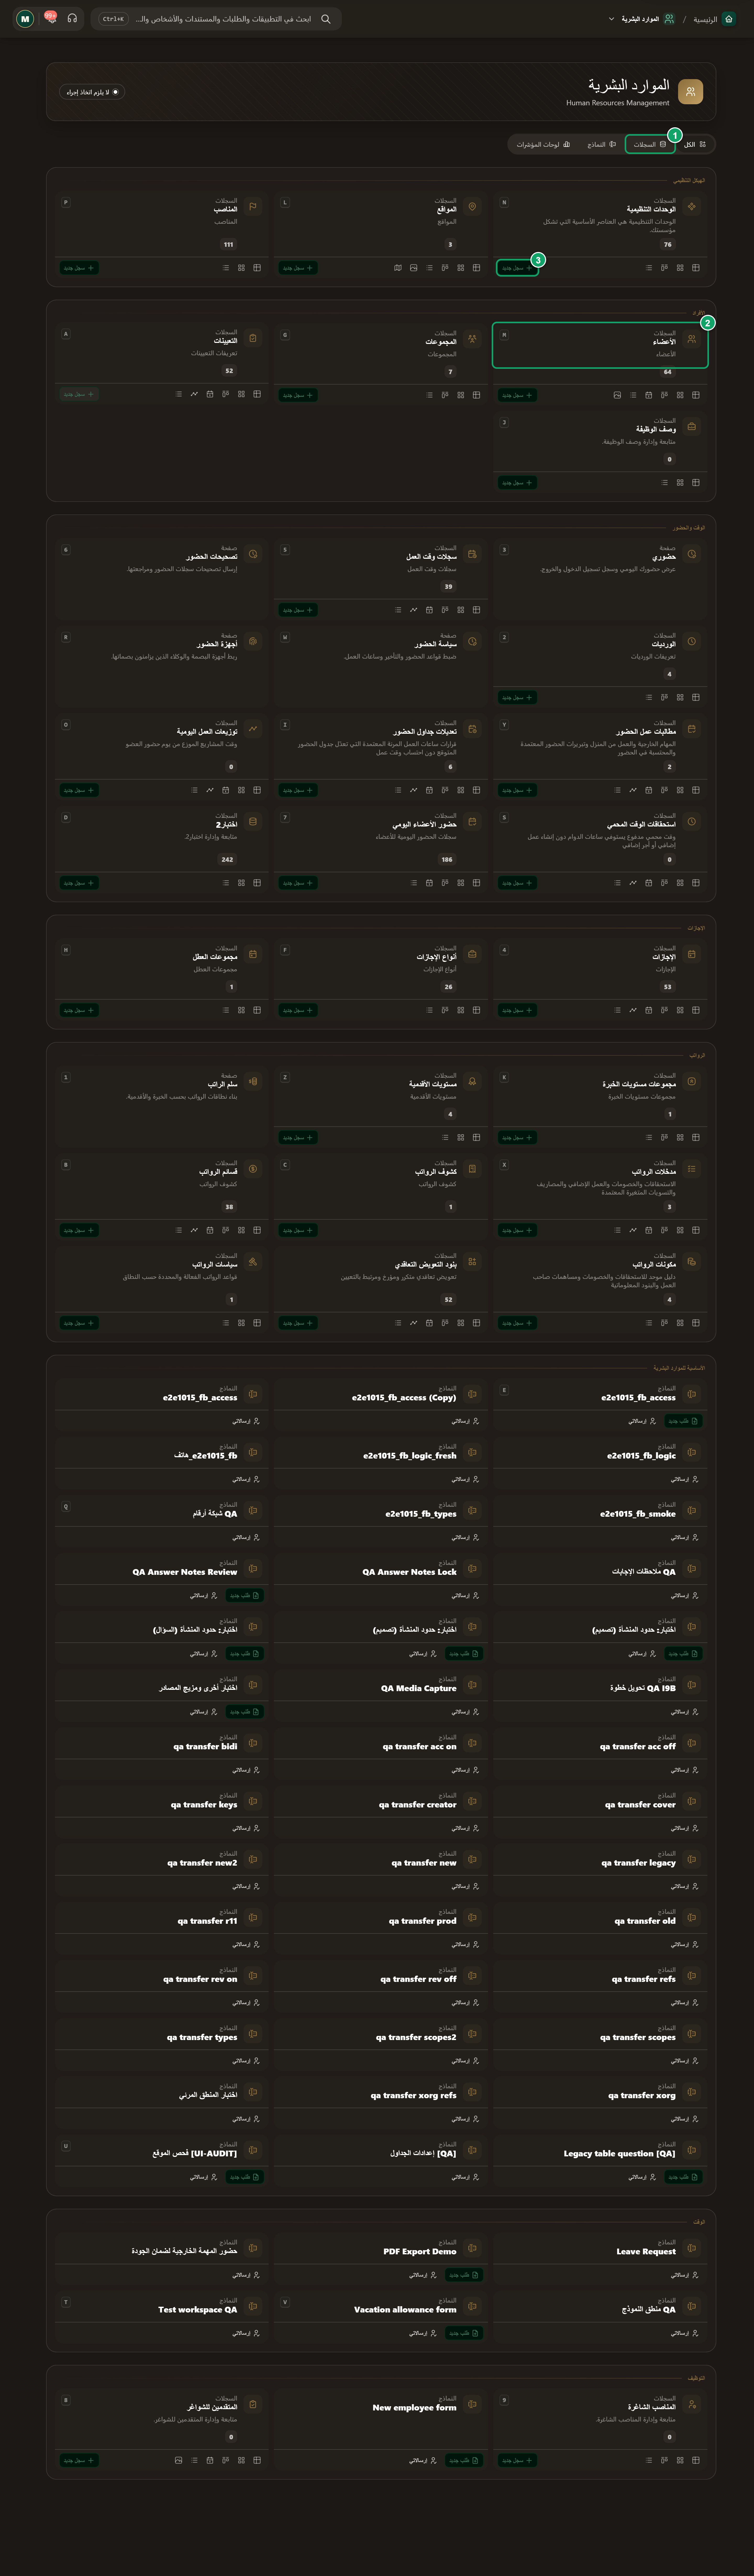
\includegraphics[width=0.95\linewidth]{figures/screens/ch03-hr-pages-clear-ar.png}
\caption{صفحات الهيكل والأشخاص}
\label{fig:hr-pages-screen}
\end{figure}

افتح الصفحات بهذا الترتيب: الأشخاص والهيكل، ثم الوقت، ثم الرواتب إن كانت مؤسستك تستخدمها. لكل صفحة شرح مستقل بالصور. \textbf{المسار:} «الموارد البشرية» / «المجموعة المذكورة مع الصفحة» / «الصفحة».

\textbf{في كل قائمة:} عرض جدول أو بطاقات أو غيرها، بحث وتصفية وعروض محفوظة، استيراد ملفات إكسل وتصديرها، وحذف جماعي؛ حسب صلاحيتك. ويذكر شرح كل صفحة ما تتميز به.

\begin{table}[H]
\centering
\caption{الأشخاص والهيكل: الأولوية الأولى}
\label{tab:hr-pages-core}
\rcZebra
\begin{tabularx}{\linewidth}{R{4.2cm} Y}
\rcHeaderRow
\thh{الصفحة ومجموعتها} & \thh{ماذا تقدم هذه الصفحة؟}\\
الأعضاء — القوى العاملة & ملف كامل لكل موظف: الهوية والاتصال والعائلة والمؤهلات والوثائق والحساب.\\
المناصب — القوى العاملة & الوظائف وتبعيتها وقسمها وموقعها ودرجتها ووردياتها.\\
التعيينات — القوى العاملة & من يشغل المنصب، ومنذ متى، وبأي عقد وراتب ووردية.\\
الوحدات التنظيمية — الأساسية & شجرة الأقسام والإدارات ومديريها.\\
النقاط الجغرافية — الأساسية & مواقع العمل وعناوينها على الخريطة.\\
المجموعات — القوى العاملة & فرق ولجان تجمع أعضاء من أقسام مختلفة.\\
\end{tabularx}
\end{table}

\begin{table}[H]
\centering
\caption{متابعة يوم العمل: صفحات الوقت}
\label{tab:hr-pages-time}
\rcZebra
\begin{tabularx}{\linewidth}{R{4.2cm} Y}
\rcHeaderRow
\thh{الصفحة ومجموعتها} & \thh{ماذا تقدم هذه الصفحة؟}\\
الورديات — الوقت & أيام العمل وساعاته واستراحاته، وكيف تصل الوردية إلى الموظف.\\
حضوري — الوقت & أيام حضورك المسجلة: الدخول والخروج والمدة.\\
جداول الدوام — الوقت & حضور الفريق لفترة تختارها.\\
أنواع الإجازات — الوقت & أنواع الإجازة وقواعدها وأثرها في الراتب.\\
الإجازات — الوقت & إجازات الموظفين: نوعها وتاريخها وحالتها.\\
مجموعات العطل الرسمية — الوقت & تقويم مشترك للعطل الرسمية، ومن يتبعه.\\
تصحيحات الحضور — الوقت & طلبات تصحيح أيام الحضور والبتّ فيها.\\
سياسة الحضور — الوقت & قواعد التأخر والخروج المبكر والعمل الإضافي.\\
أجهزة الحضور — الوقت & أجهزة البصمة وربط مستخدميها بالأعضاء.\\
\end{tabularx}
\end{table}

\begin{table}[H]
\centering
\caption{عند احتساب الرواتب: الإعداد ثم المراجعة}
\label{tab:hr-pages-pay}
\rcZebra
\begin{tabularx}{\linewidth}{R{4.2cm} Y}
\rcHeaderRow
\thh{الصفحة ومجموعتها} & \thh{ماذا تقدم هذه الصفحة؟}\\
المستويات الوظيفية — سلم الراتب & الدرجات الوظيفية وحدود رواتبها.\\
مستويات الخبرة — سلم الراتب & مجموعات الخبرة ومستوياتها وزياداتها.\\
سلم الراتب — سلم الراتب & جدول الرواتب المرجعية لكل درجة ومستوى خبرة.\\
مدخلات الرواتب — الدفع & بنود الشهر المتغيرة: مكافأة، خصم، عمل إضافي.\\
قسائم الرواتب — الدفع & حساب راتب كل موظف واعتماده.\\
كشوف الرواتب — الدفع & كشف رواتب الشهر من القسائم المعتمدة.\\
\end{tabularx}
\end{table}

% Dedicated HR feature pages. Shared source for HTML, PDF and Word.
% كل صفحة: ما هي، المسار، صورة، ما الذي تسجله (كل التبويبات)، ما الذي يمكنك فعله، مخطط، خطوات وتحقق.

\clearpage
\section{الأعضاء}
\label{sec:hr-feature-members}

العضو هو الشخص الذي يعمل في المؤسسة. يجمع سجلّه بياناته الشخصية ووسائل الاتصال به ومؤهلاته وبياناته المالية. ويربطه التعيين بمنصبه.

\textbf{متى تفيد؟} يبقى ملف سارة واحداً طوال عملها، حتى إذا تغيّر منصبها. \textbf{المسار:} «الموارد البشرية» / «القوى العاملة» / «الأعضاء».

\begin{figure}[H]
\centering
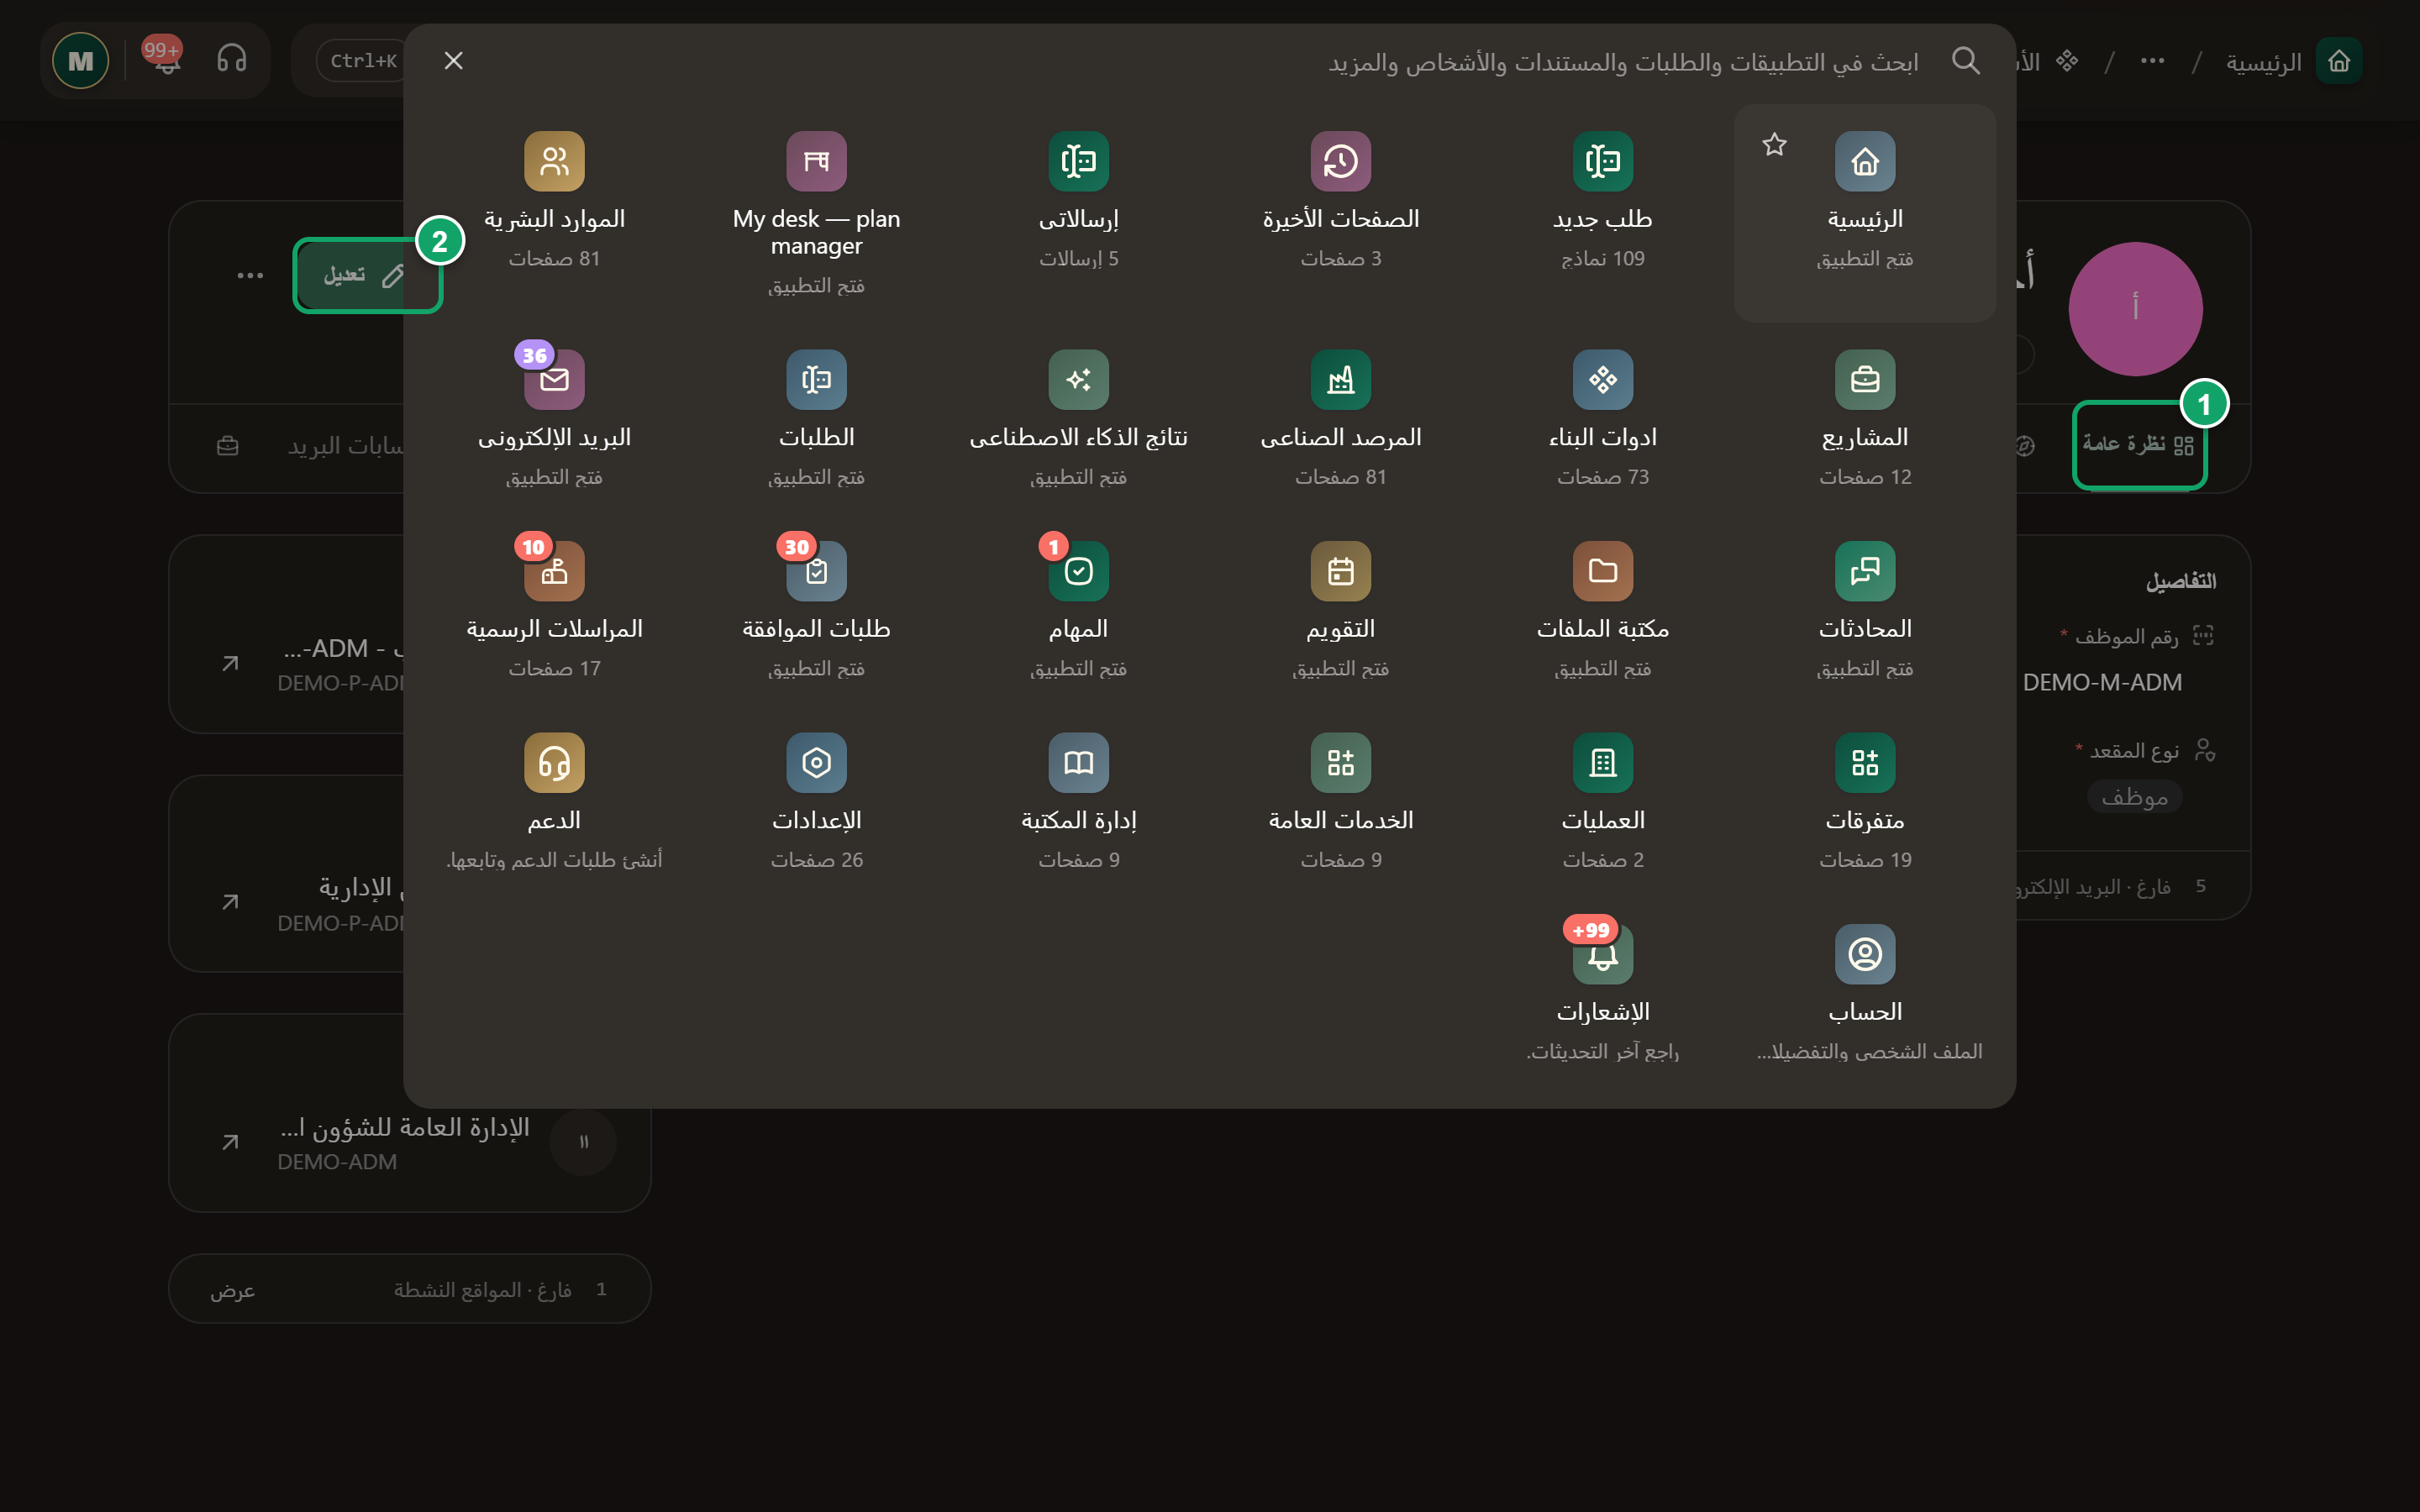
\includegraphics[width=0.95\linewidth]{figures/screens/ch02-member-fields-ar.png}
\caption{الأعضاء: ملف موظف تجريبي؛ يختلف عن مثال سارة}
\label{fig:hr-feature-members-screen}
\end{figure}

\begin{table}[H]
\centering
\caption{ما الذي تسجله في ملف العضو؟}
\label{tab:hr-feature-members-data}
\rcZebra
\begin{tabularx}{\linewidth}{R{3.6cm} Y}
\rcHeaderRow
\thh{التبويب أو القسم} & \thh{ما الذي تضيفه؟}\\
البيانات الرئيسية & رقم الموظف \req{} والاسم \req{}، والبريد والهاتف والصورة، و«التسجيل» (السماح بالدخول)، واللغة المفضلة والمنطقة الزمنية، ورقم البصمة.\\
الشخصي & اسم الأب واسم الأم، والجنس، والحالة الاجتماعية، وزمرة الدم، وتاريخ الميلاد ومكانه، والجنسية، والرقم الوطني وملفه، والسيرة الذاتية، وجواز السفر، ورخصة القيادة، ومعلومات العائلة.\\
الاتصال & العنوان وسند الإقامة، وأرقام الهاتف الشخصي والعمل والمنزل، والبريد الشخصي وبريد العمل، وجهات اتصال الطوارئ.\\
المؤهلات & التعليم، والمهارات ومستوى إتقانها، واللغات، والتدريبات، والخبرات السابقة؛ مع شهاداتها.\\
تضارب المصالح & الأقارب في المؤسسة، وجهة عمل أخرى، والتضارب مع الموردين أو الشركاء؛ مع القرار المتخذ وحالته.\\
المالية & الحسابات البنكية، وتأمين الموظف، والمكافآت والخصومات، وكشوف الرواتب.\\
التوظيف والحضور & تعيينات العضو، ورصيد إجازاته وسجل إجازاته.\\
تبويبات الحساب & حسابات البريد، والإشعارات وساعات الهدوء، والجلسات، والتحقق بخطوتين، والأجهزة المرتبطة (إن كانت الميزة مفعّلة).\\
\end{tabularx}
\end{table}

هذه هي الحقول الافتراضية، وقد يعدّلها مسؤول مؤسستك. يملأ النظام حقلي المناصب والوحدات النشطة \gen{} من التعيينات.

\subsection{ما الذي يمكنك فعله؟}

\begin{itemize}
  \item «إضافة تعيين» من ملف العضو؛ يظهر فيه العضو مختاراً مسبقاً.
  \item «تغيير كلمة المرور»، مع خيار إلزامه بتغييرها عند دخوله التالي.
  \item «إنهاء ارتباط العضو»: اختر لمسؤولياته «نقل» إلى موظف بديل أو «إلغاء إسناد» أو «الإبقاء»، وحدد تاريخ السريان، وراجع ما سيتأثر.
  \item في القائمة بطاقات تعرض إجمالي الأعضاء، ومن لديهم تعيينات نشطة، ومن ليست لديهم.
\end{itemize}

\begin{figure}[H]
\centering
\begin{tikzpicture}[node distance=0.5cm,stepBox/.append style={minimum width=6.5cm,text width=6.1cm,minimum height=0.8cm}]
  \node[stepBox] (a) {\RL{إنشاء سجل سارة}};
  \node[stepBox,below=of a] (b) {\RL{التعيين الوظيفي}};
  \node[stepBox,below=of b] (c) {\RL{مراجعة الوظيفة}\\\RL{والفترة}};
  \draw[flowsTo] (a) -- (b);
  \draw[flowsTo] (b) -- (c);
\end{tikzpicture}
\rclegend
\caption{خطوات الاستخدام؛ الأسهم لا تعني معالجة تلقائية}
\label{fig:hr-feature-members-flow}
\end{figure}

\subsection{جرّب وراجع}

\begin{enumerate}
  \item افتح «الأعضاء» وابحث عن سارة قبل إضافة سجل جديد، لتجنب التكرار.
  \item أضف رقم الموظف \en{0001} والاسم «سارة الخطيب» والبريد، ثم «حفظ».
  \item افتح تبويب «الاتصال» وأضف جهة اتصال طوارئ بالاسم والهاتف والعلاقة، ثم احفظ.
  \item من قائمة إجراءات السجل اختر «إضافة تعيين» واربطها بمنصبها.
\end{enumerate}

\textbf{تحقق:} أعد فتح السجل وراجع التبويبات. تظهر وظيفتها في تبويب «التوظيف» بعد حفظ التعيين.

\subsection{تبويبات ملف الموظف}

\begin{figure}[H]
\centering
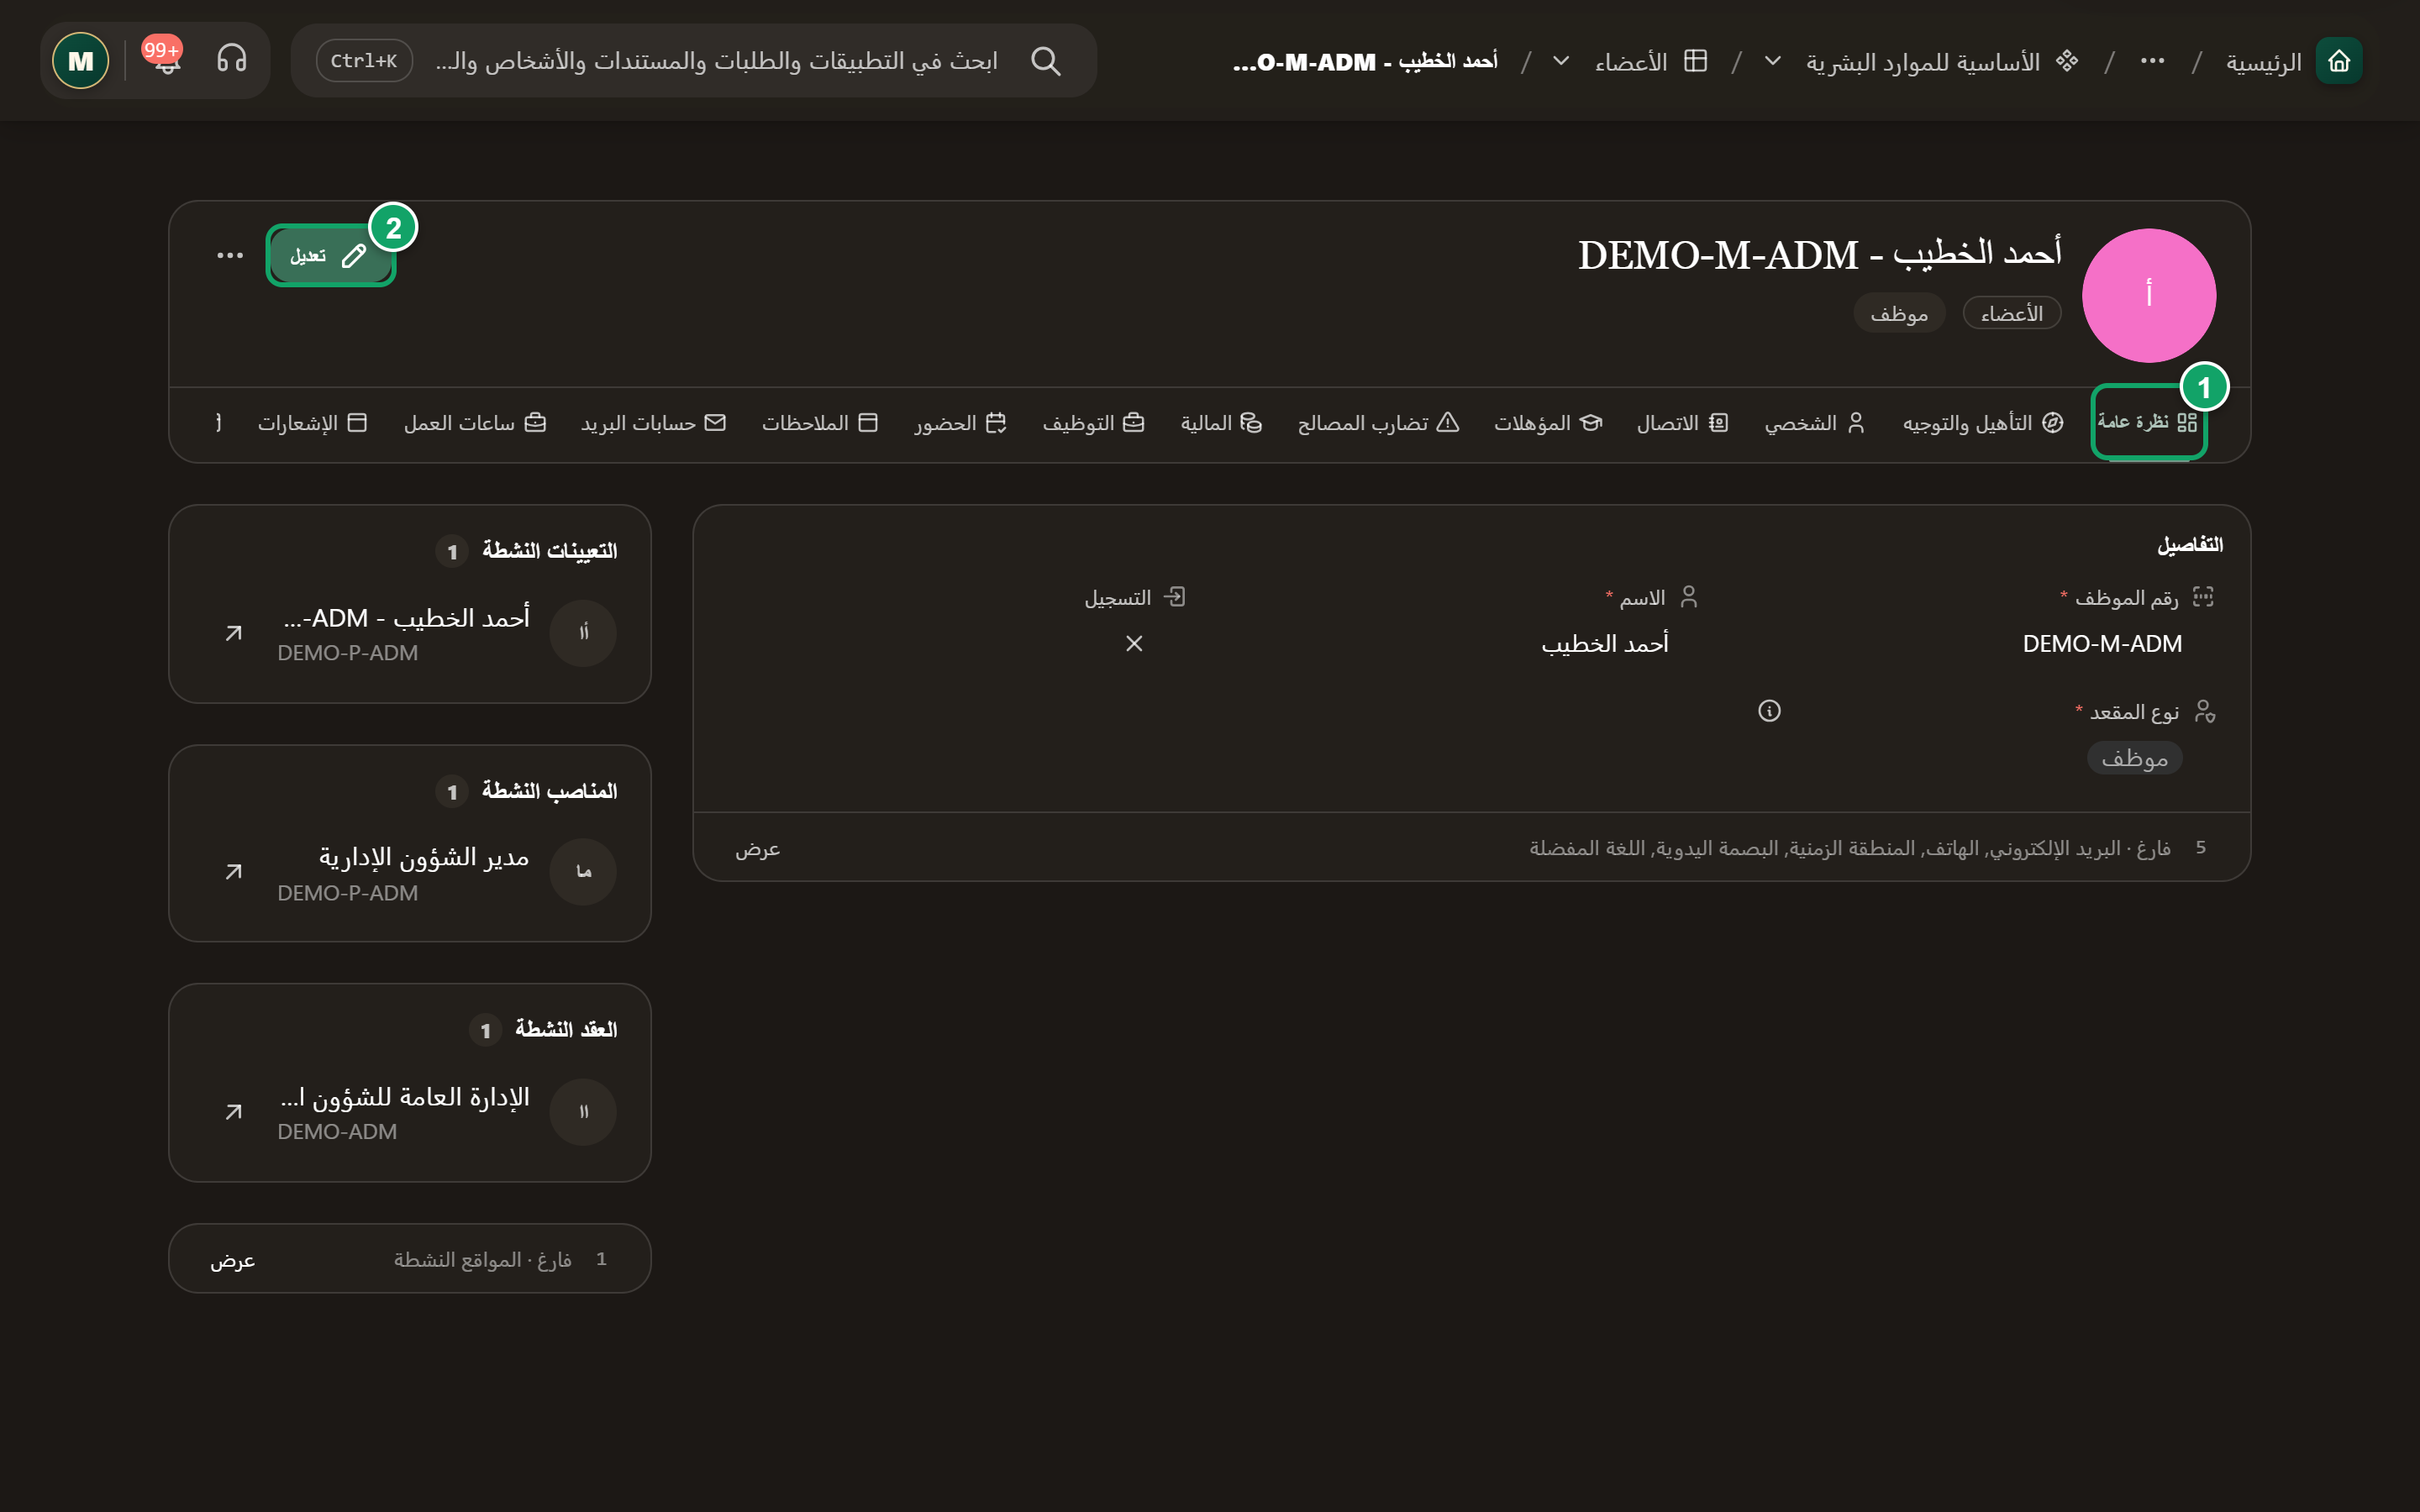
\includegraphics[width=0.95\linewidth]{figures/screens/ch03-member-tab1-ar.png}
\caption{ملف الموظف التجريبي — تبويب «نظرة عامة»}
\label{fig:hr-member-tab1}
\end{figure}

\begin{figure}[H]
\centering
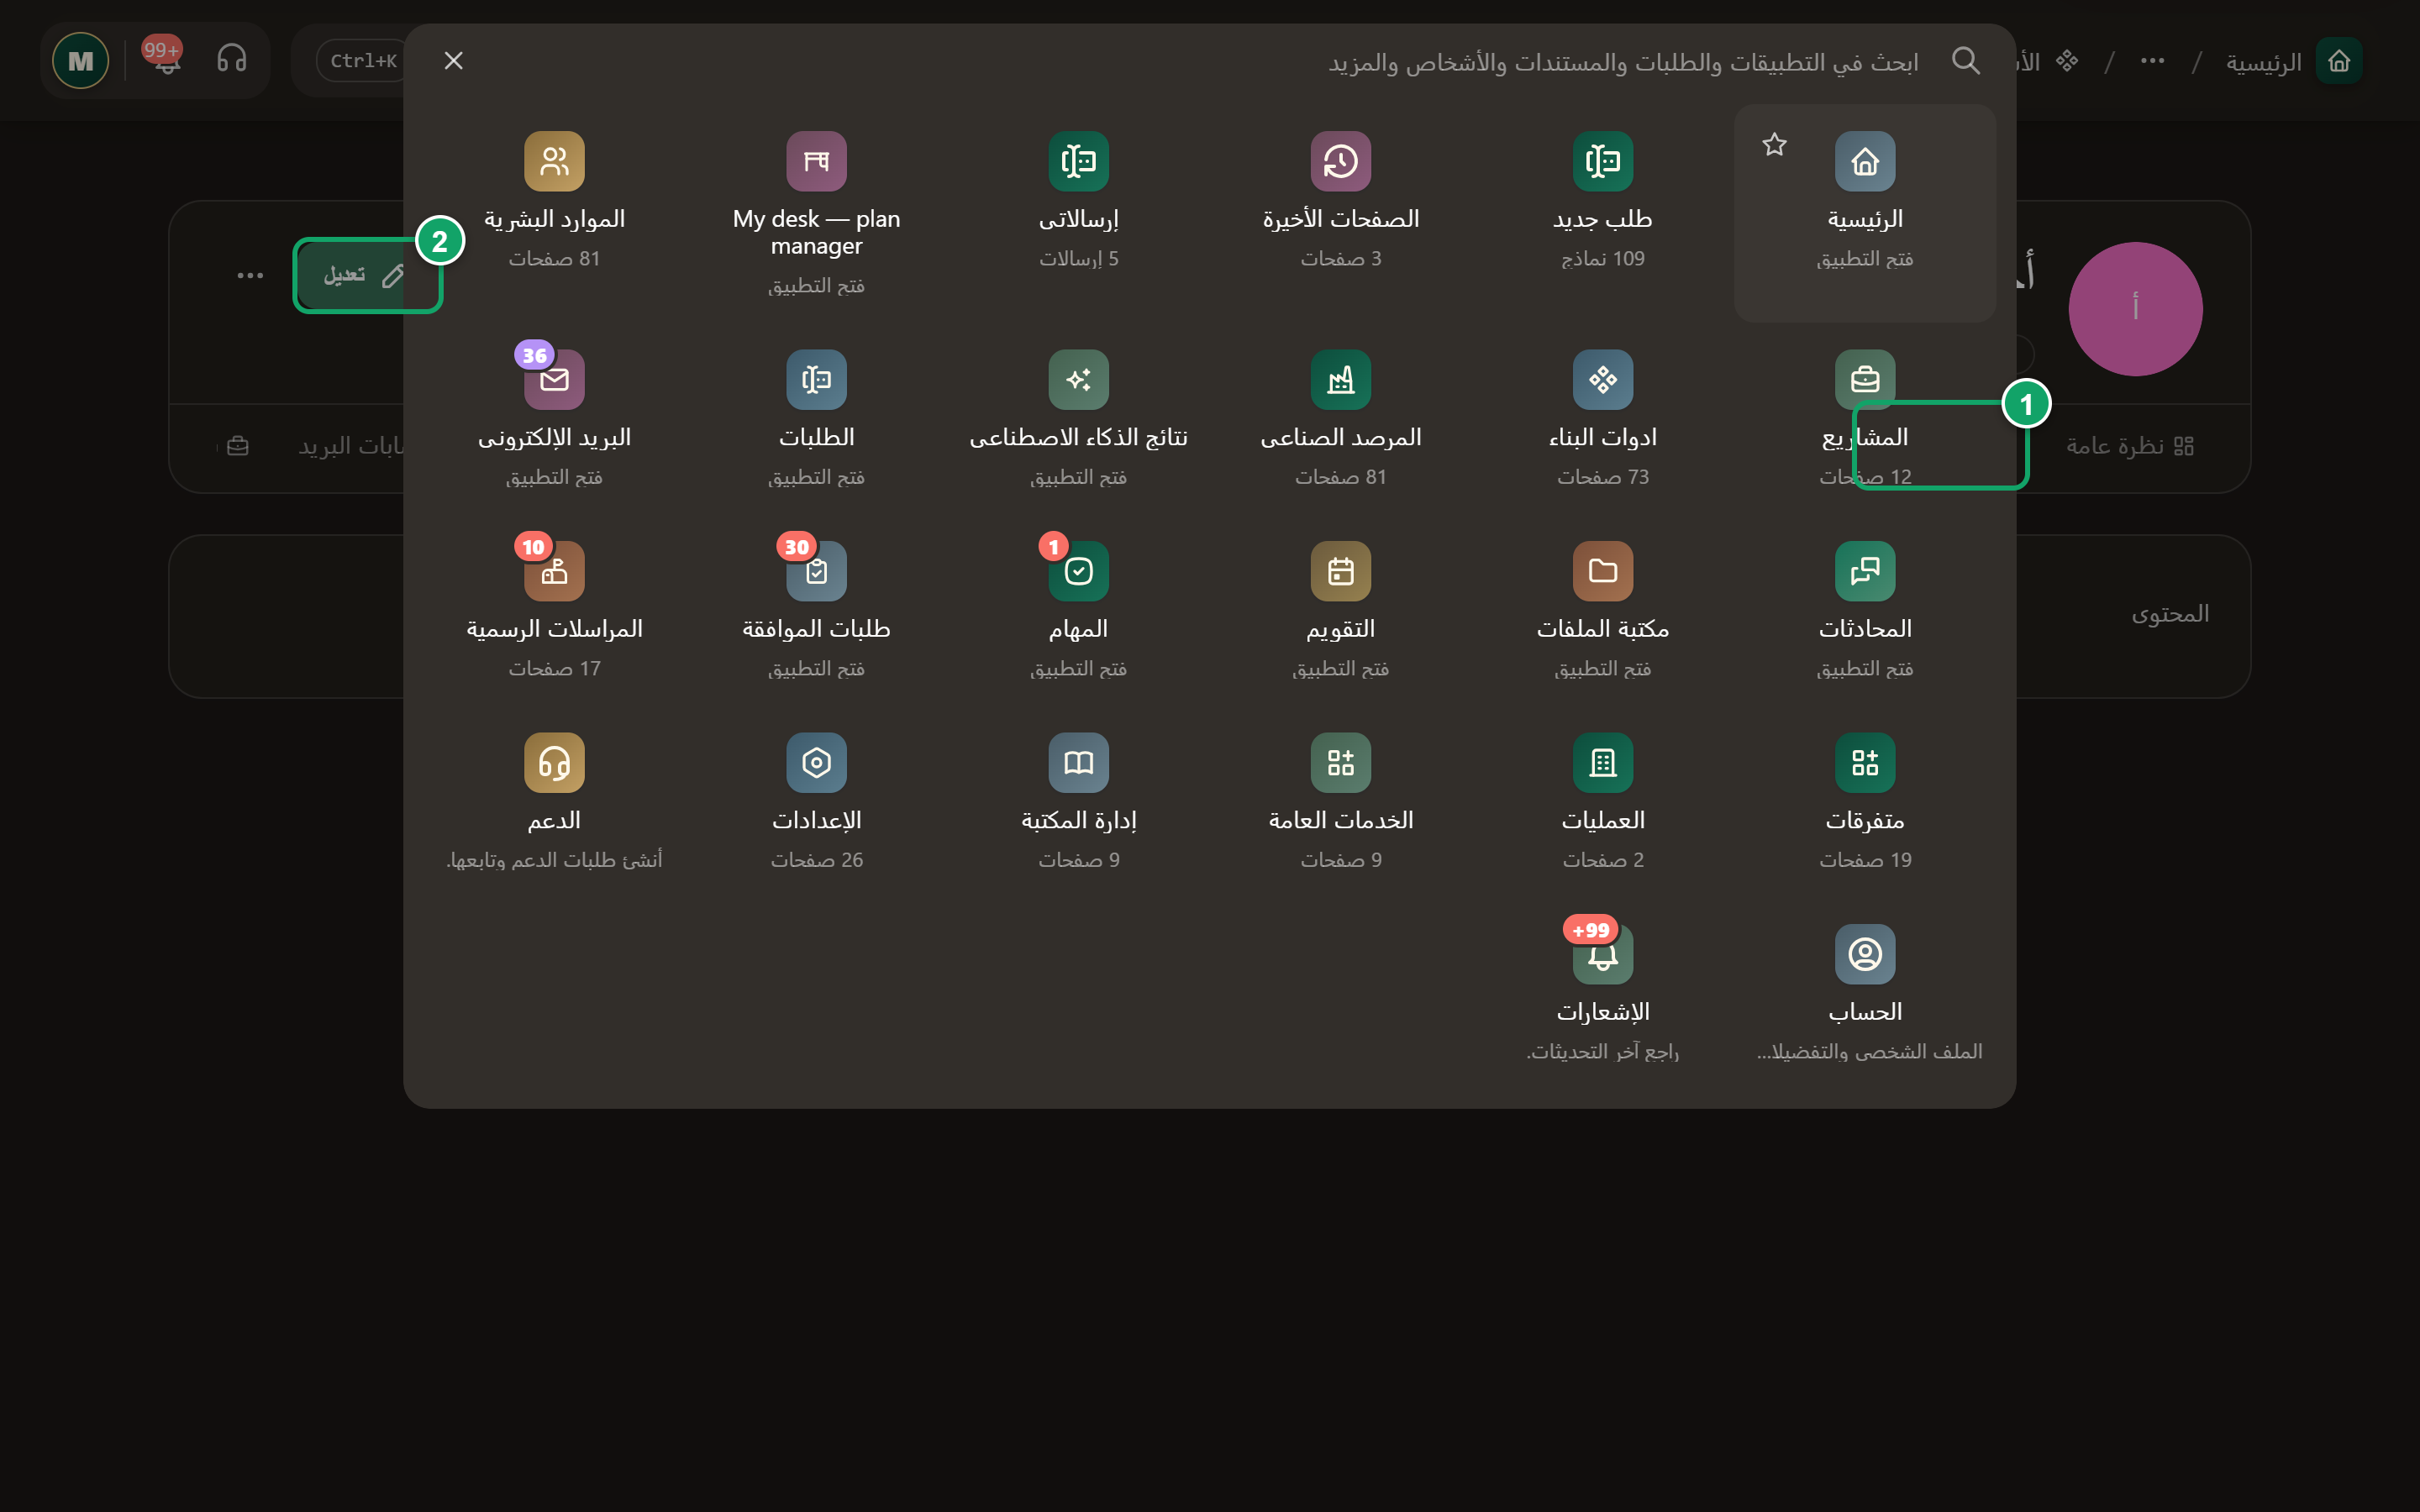
\includegraphics[width=0.95\linewidth]{figures/screens/ch03-member-tab2-ar.png}
\caption{ملف الموظف التجريبي — تبويب «التأهيل والتوجيه»}
\label{fig:hr-member-tab2}
\end{figure}

\begin{figure}[H]
\centering
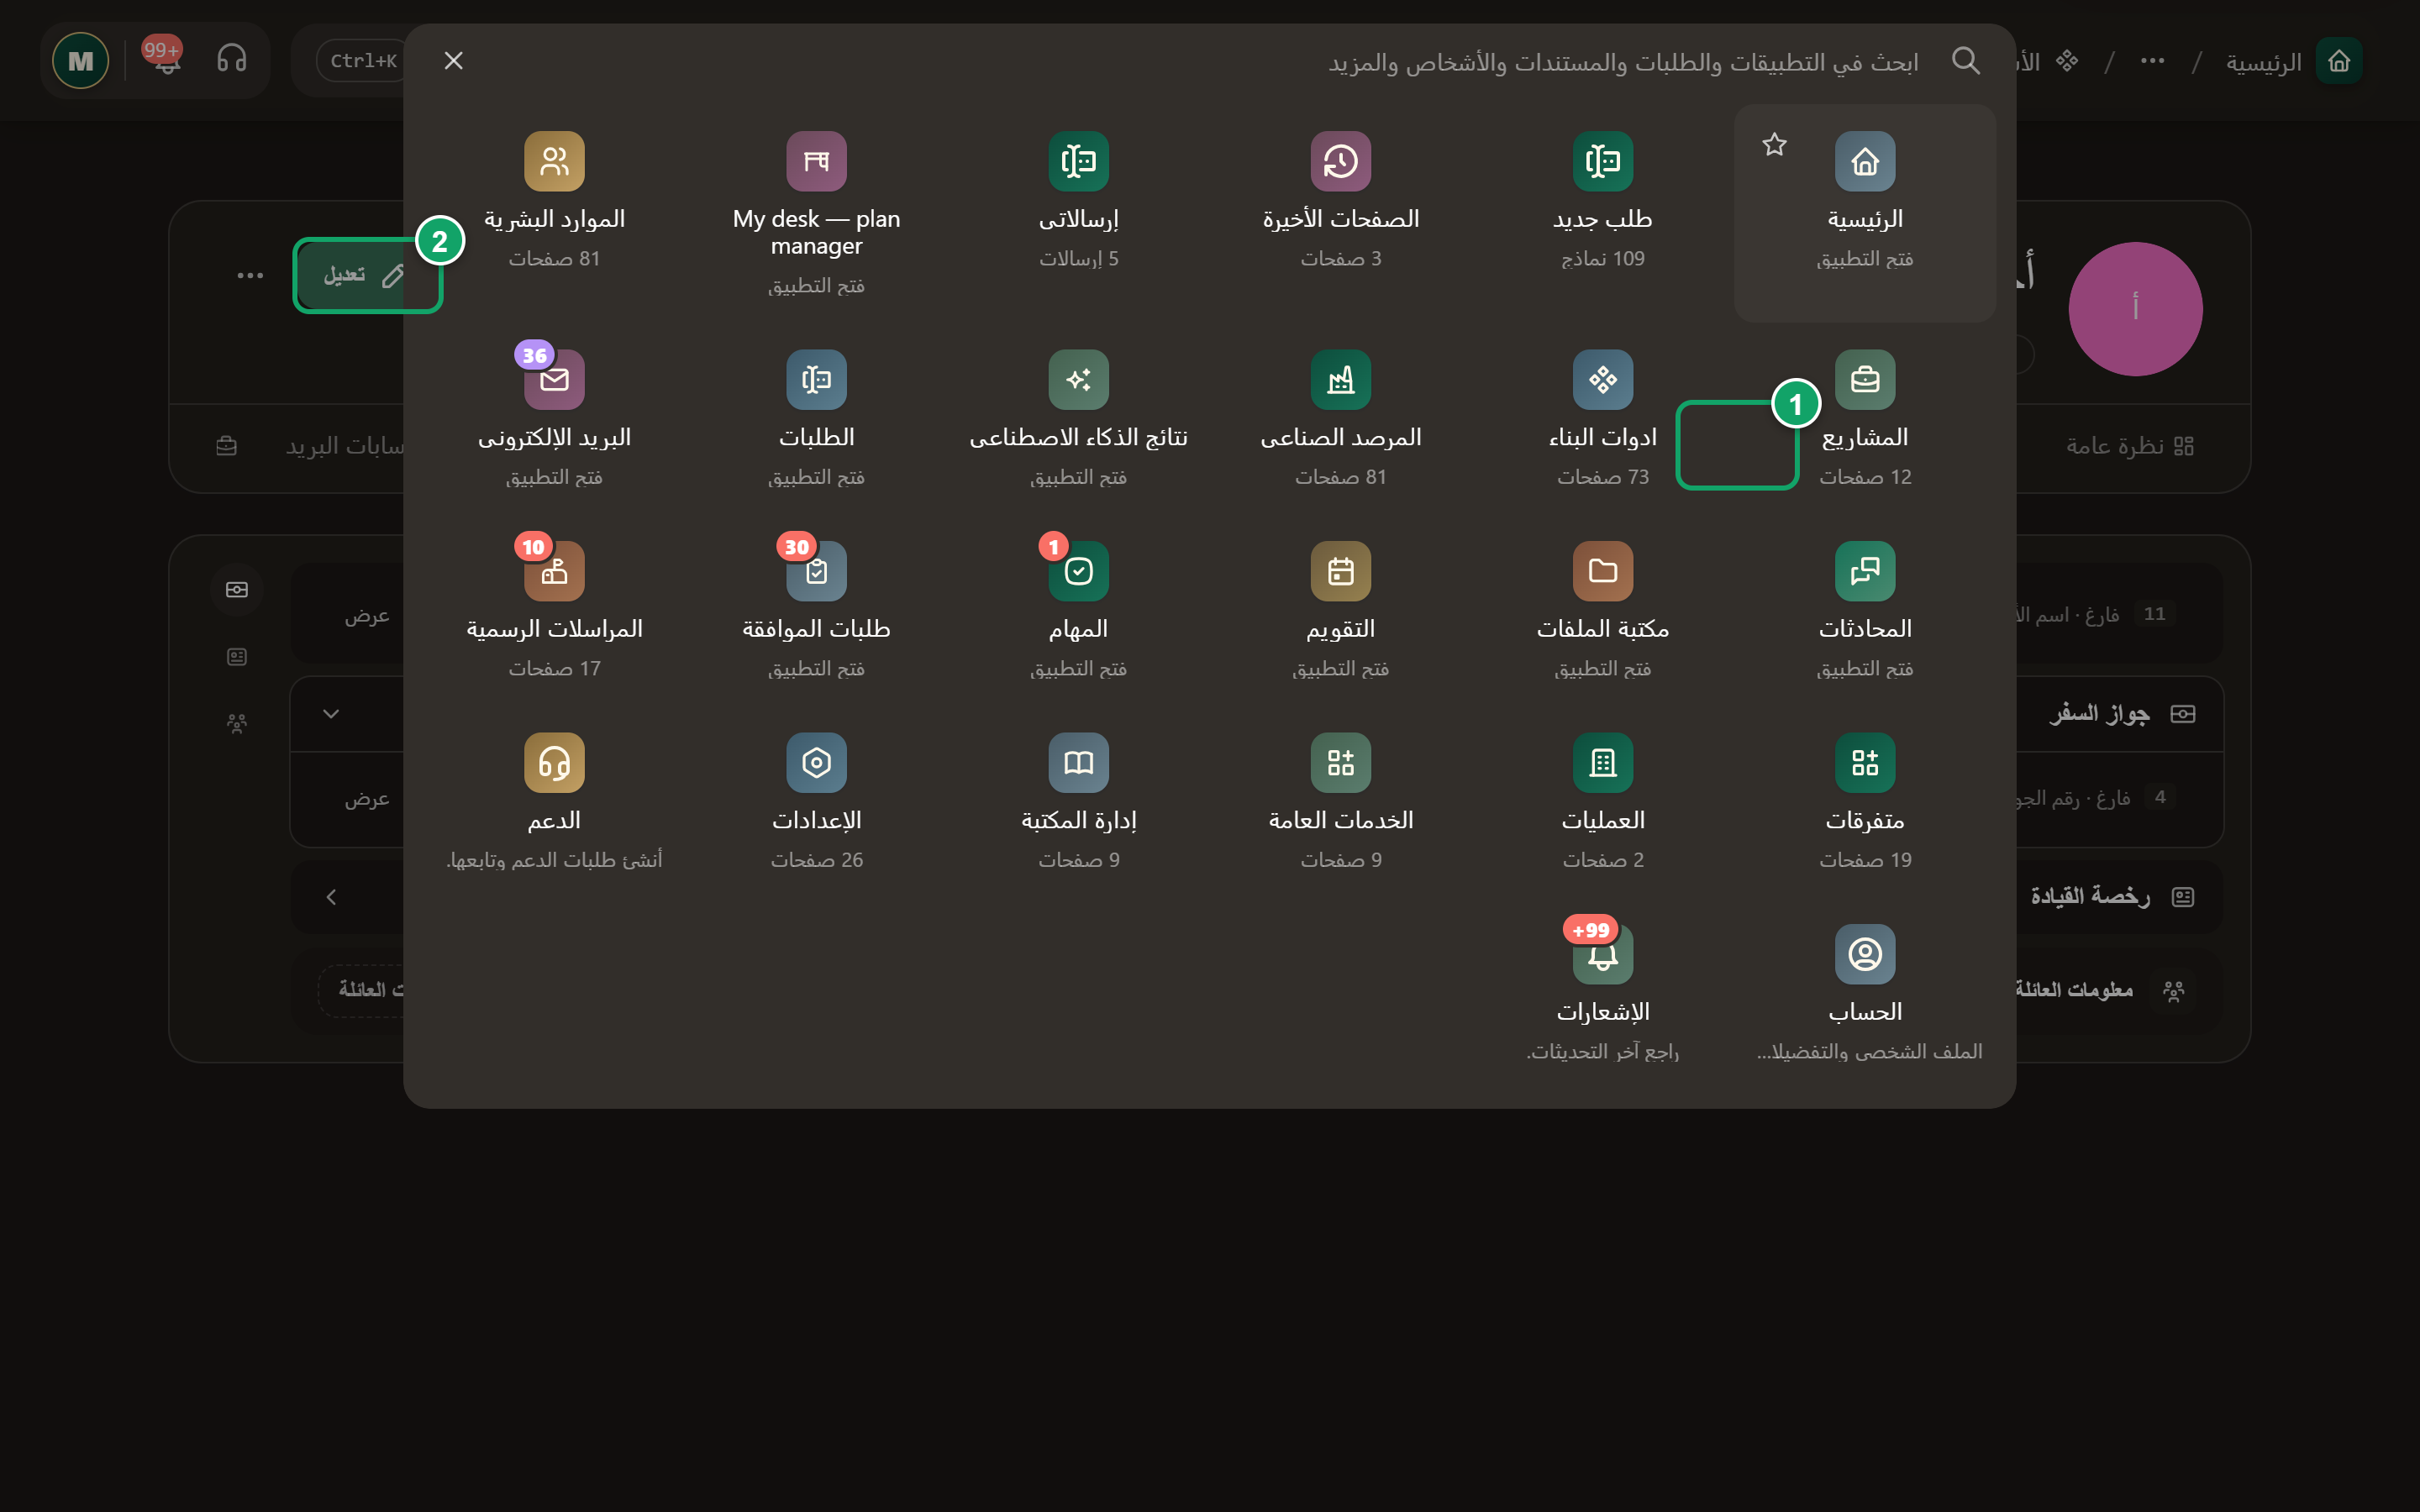
\includegraphics[width=0.95\linewidth]{figures/screens/ch03-member-tab3-ar.png}
\caption{ملف الموظف التجريبي — تبويب «الشخصي»}
\label{fig:hr-member-tab3}
\end{figure}

\begin{figure}[H]
\centering
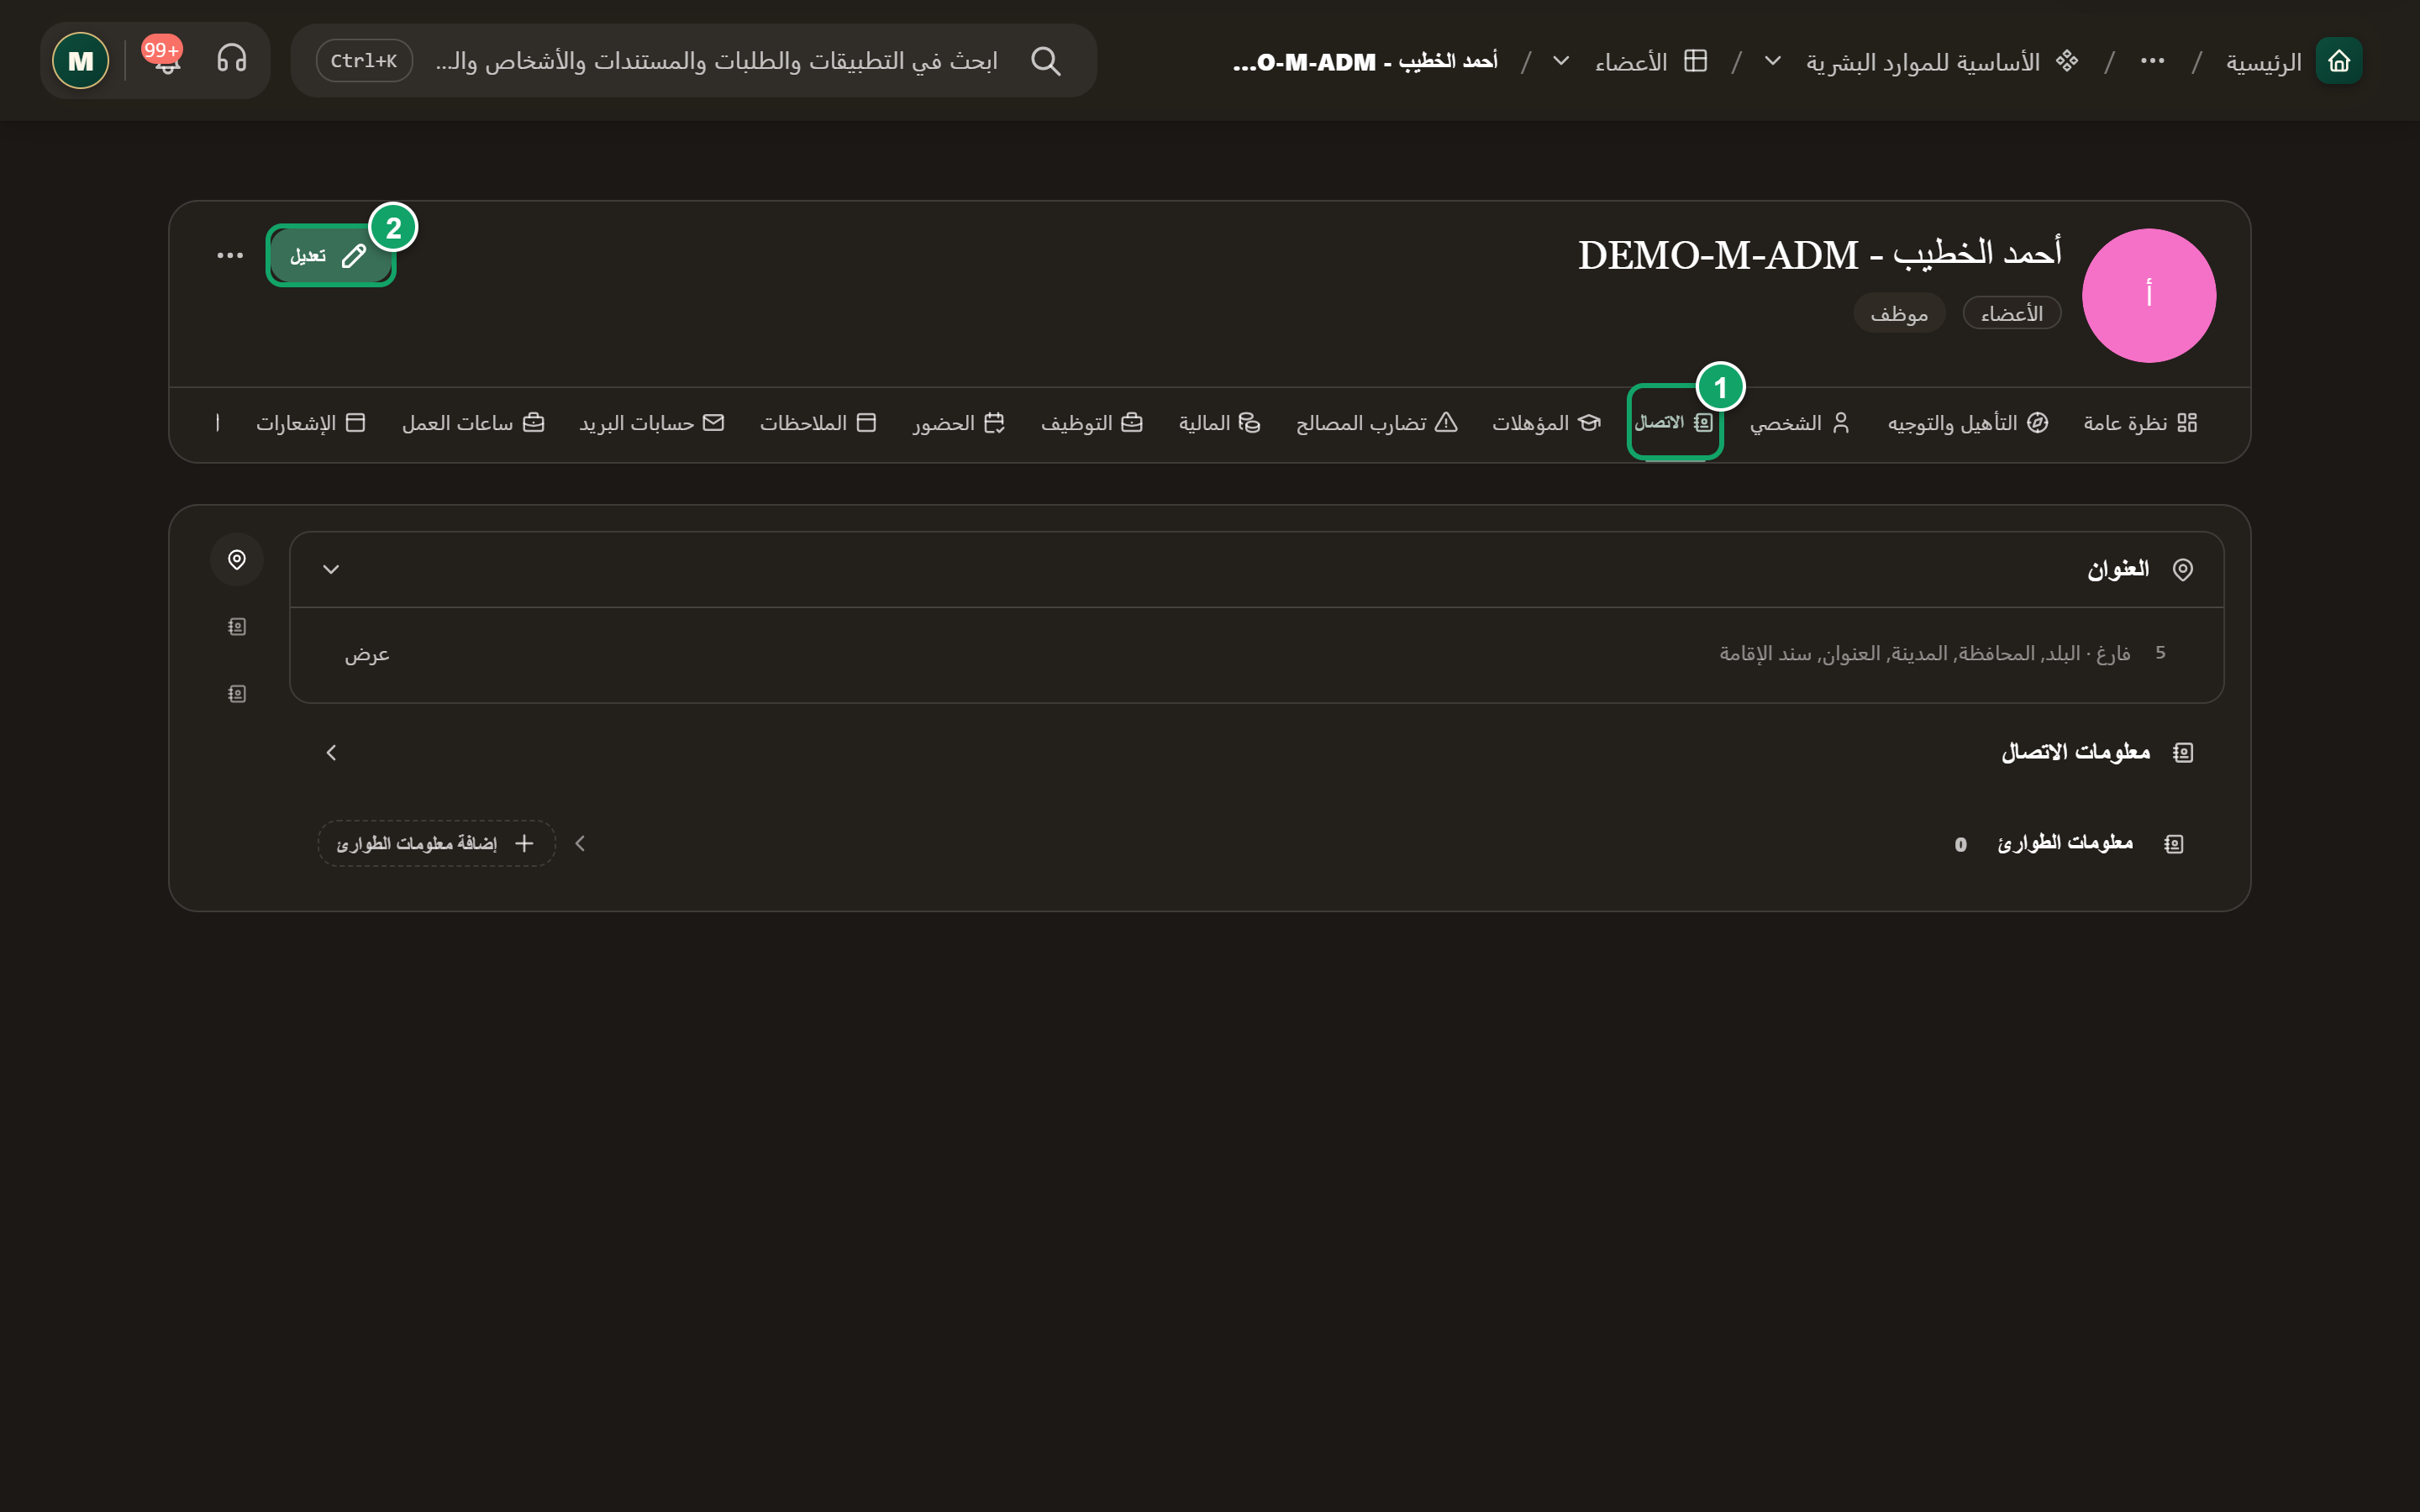
\includegraphics[width=0.95\linewidth]{figures/screens/ch03-member-tab4-ar.png}
\caption{ملف الموظف التجريبي — تبويب «الاتصال»}
\label{fig:hr-member-tab4}
\end{figure}

\begin{figure}[H]
\centering
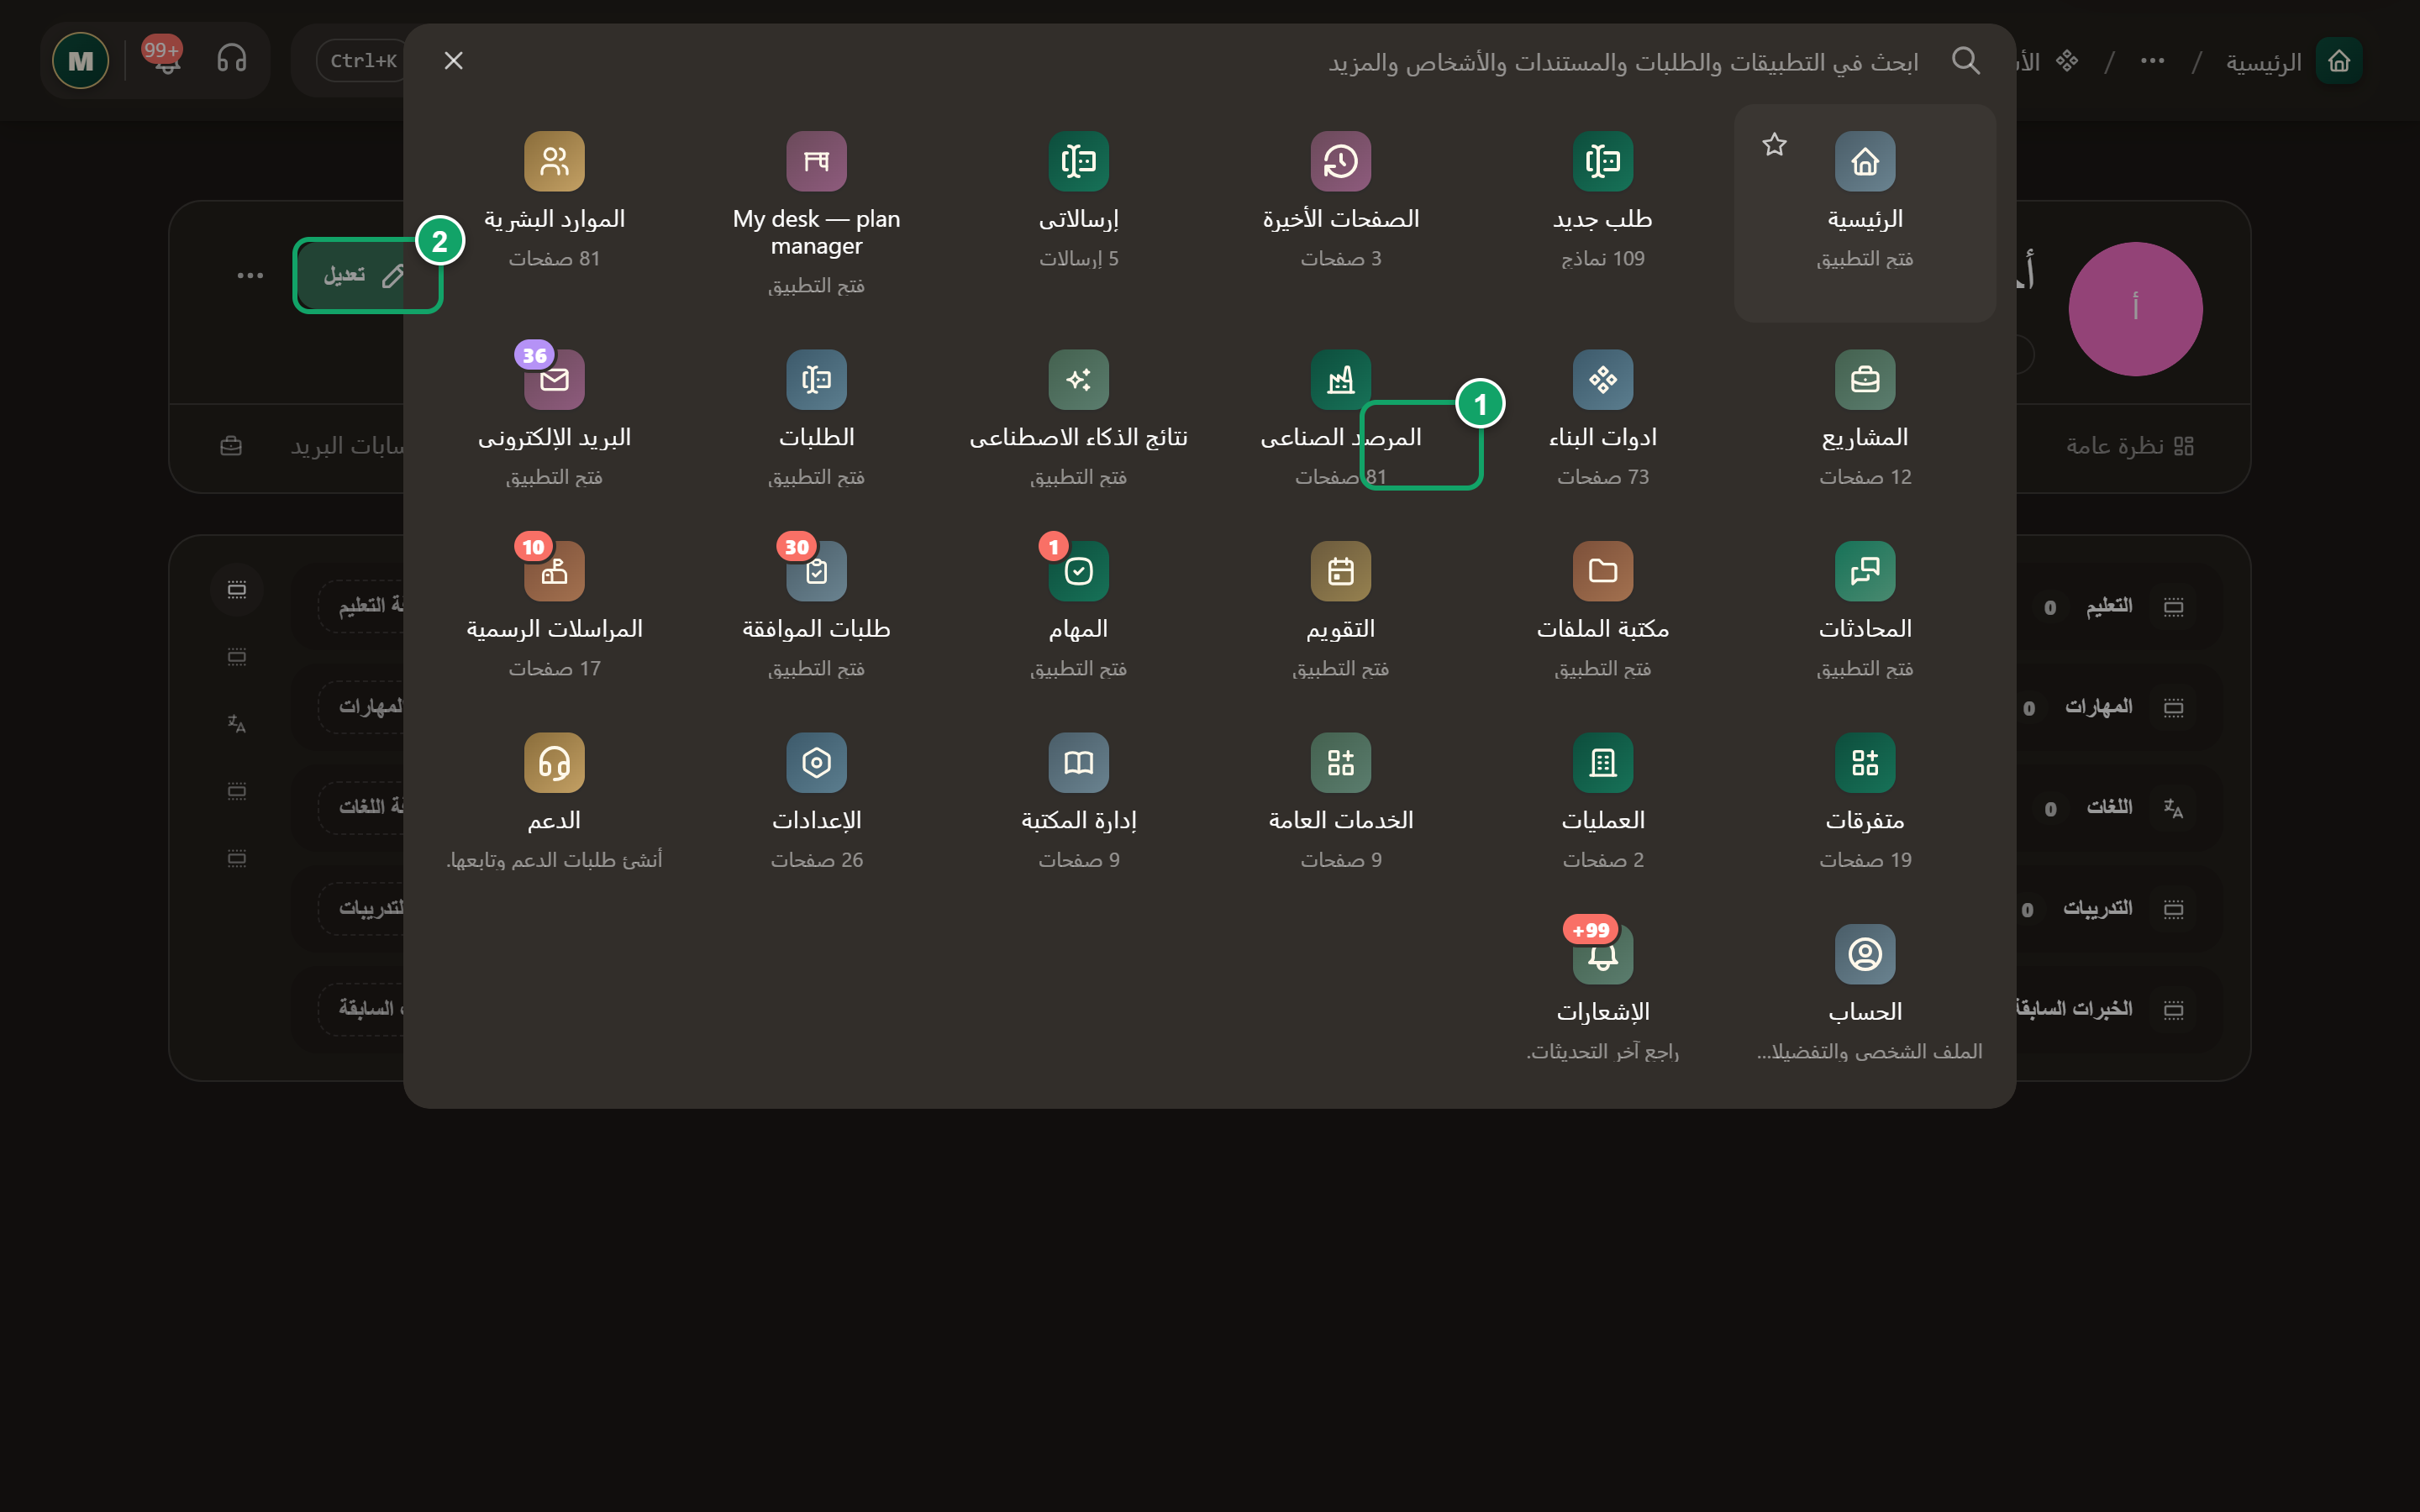
\includegraphics[width=0.95\linewidth]{figures/screens/ch03-member-tab5-ar.png}
\caption{ملف الموظف التجريبي — تبويب «المؤهلات»}
\label{fig:hr-member-tab5}
\end{figure}

\begin{figure}[H]
\centering
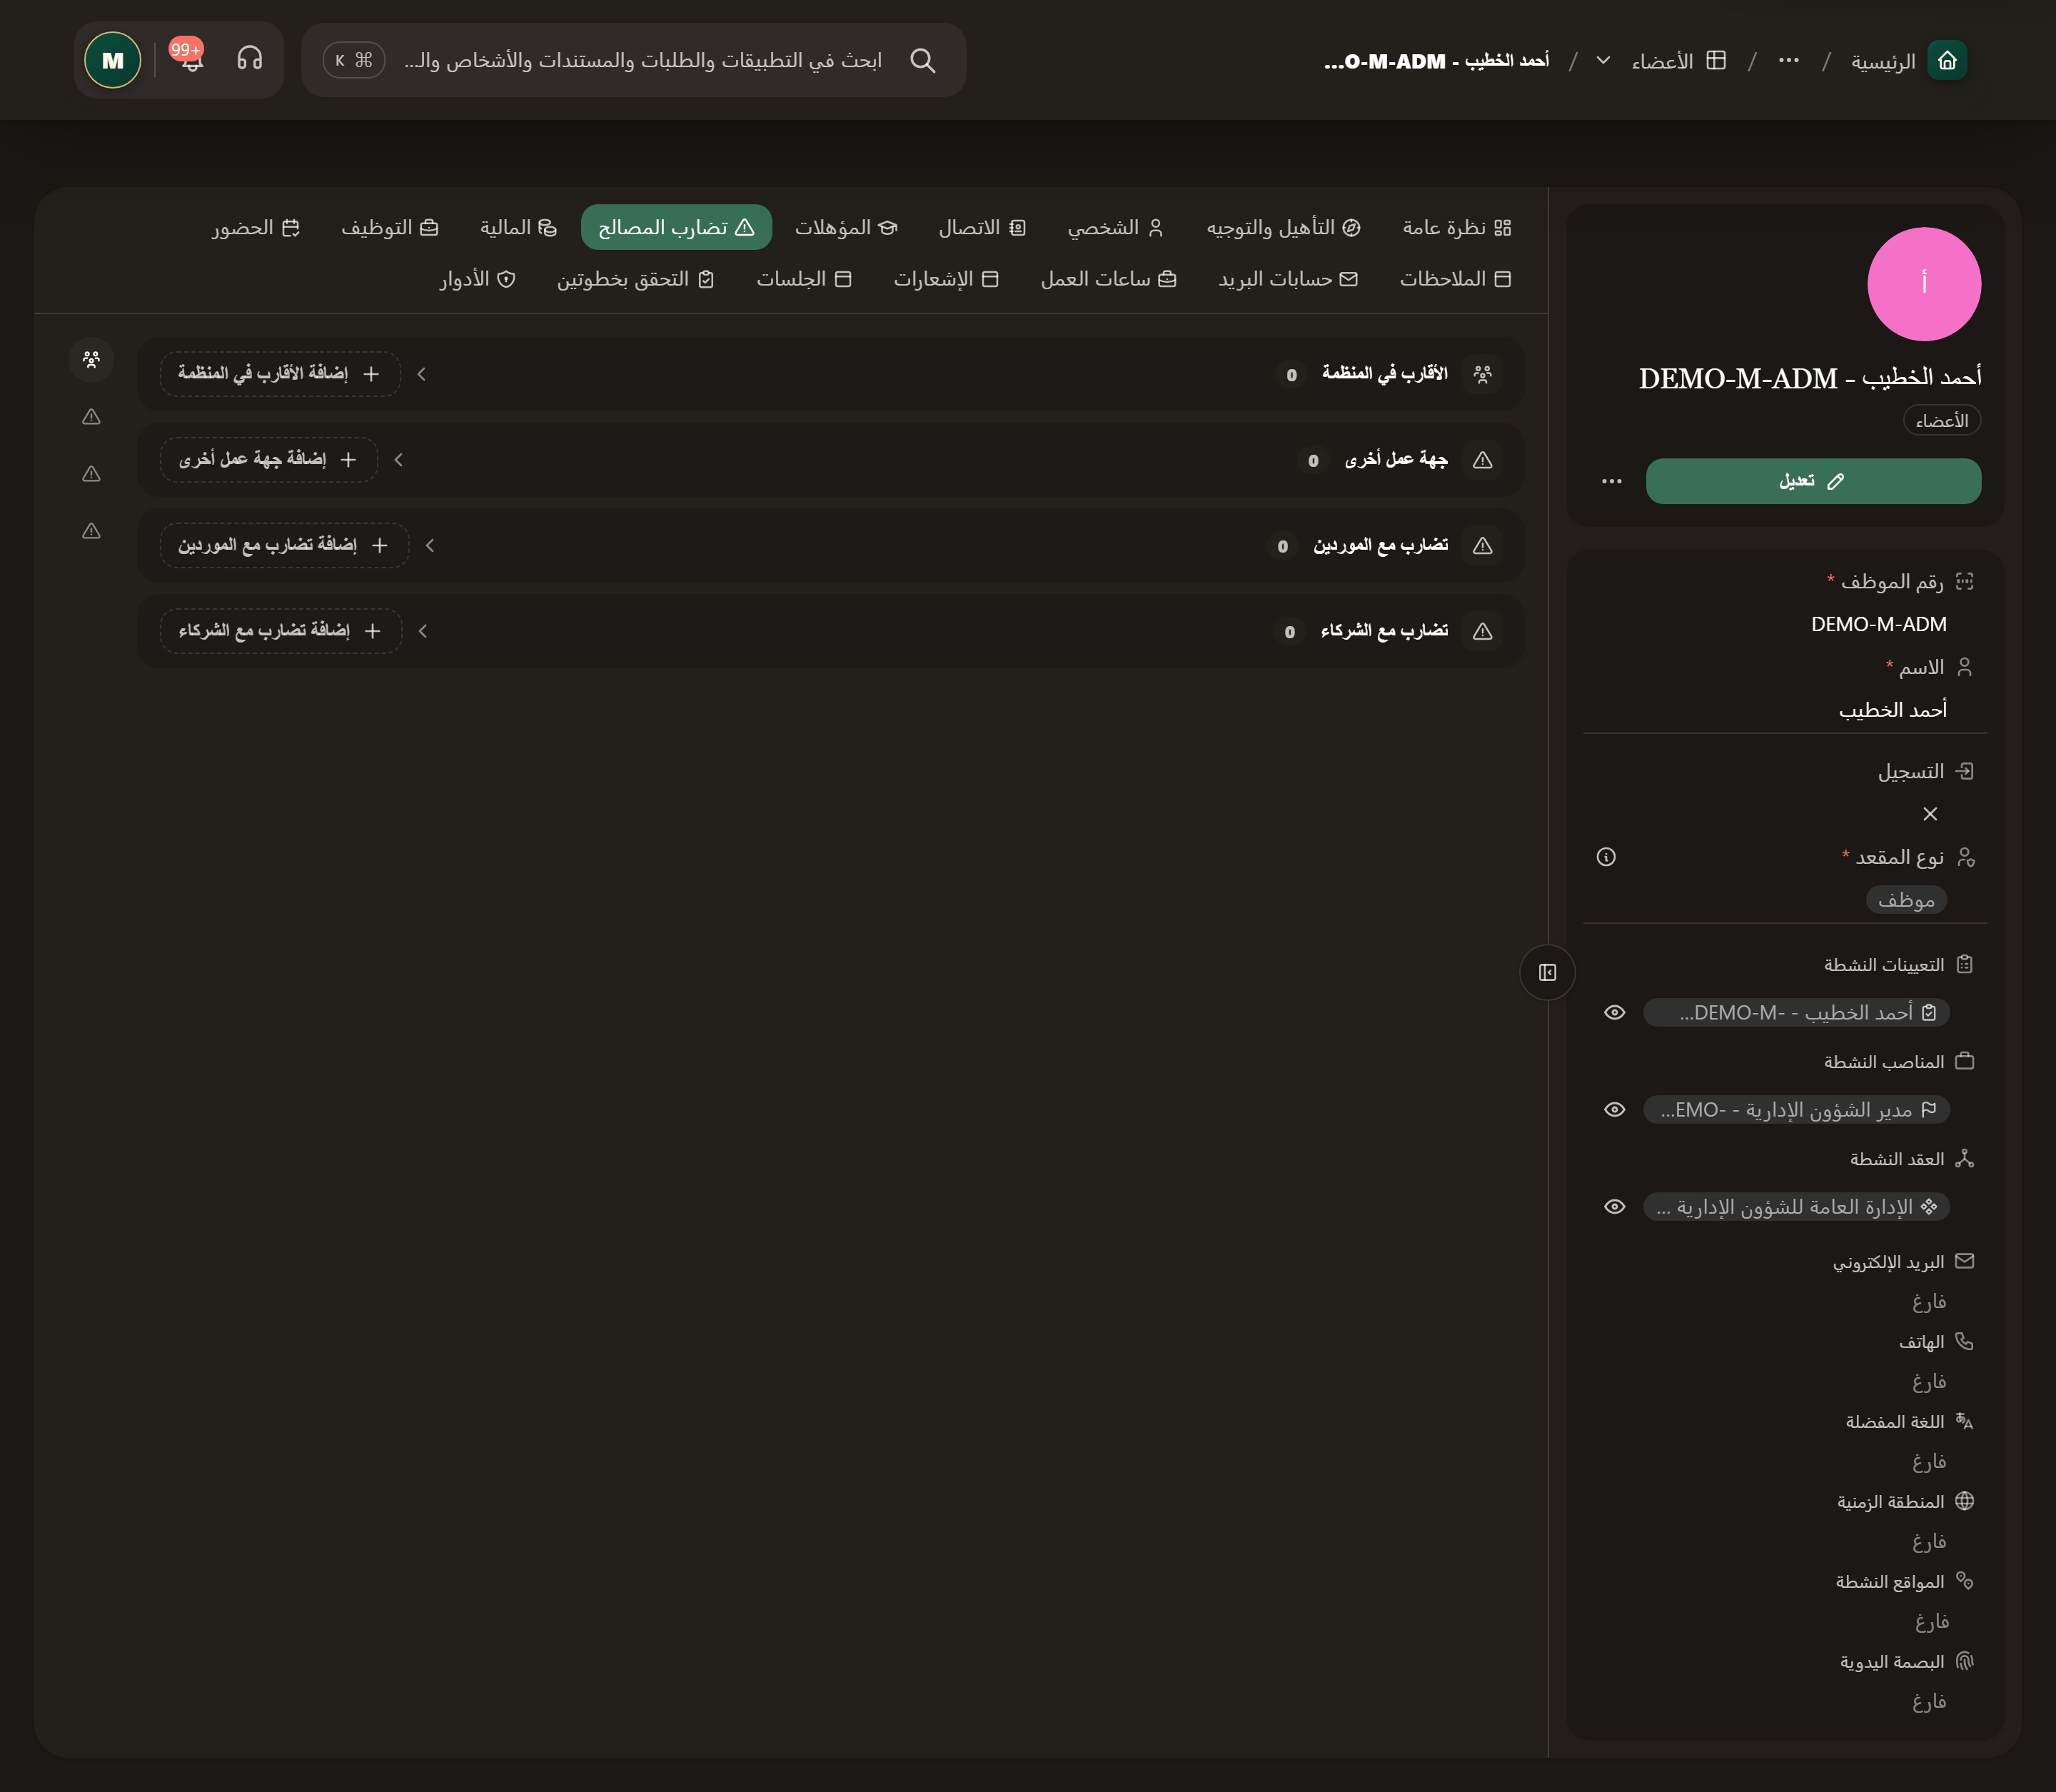
\includegraphics[width=0.95\linewidth]{figures/screens/ch03-member-tab6-ar.png}
\caption{ملف الموظف التجريبي — تبويب «تضارب المصالح»}
\label{fig:hr-member-tab6}
\end{figure}

\begin{figure}[H]
\centering
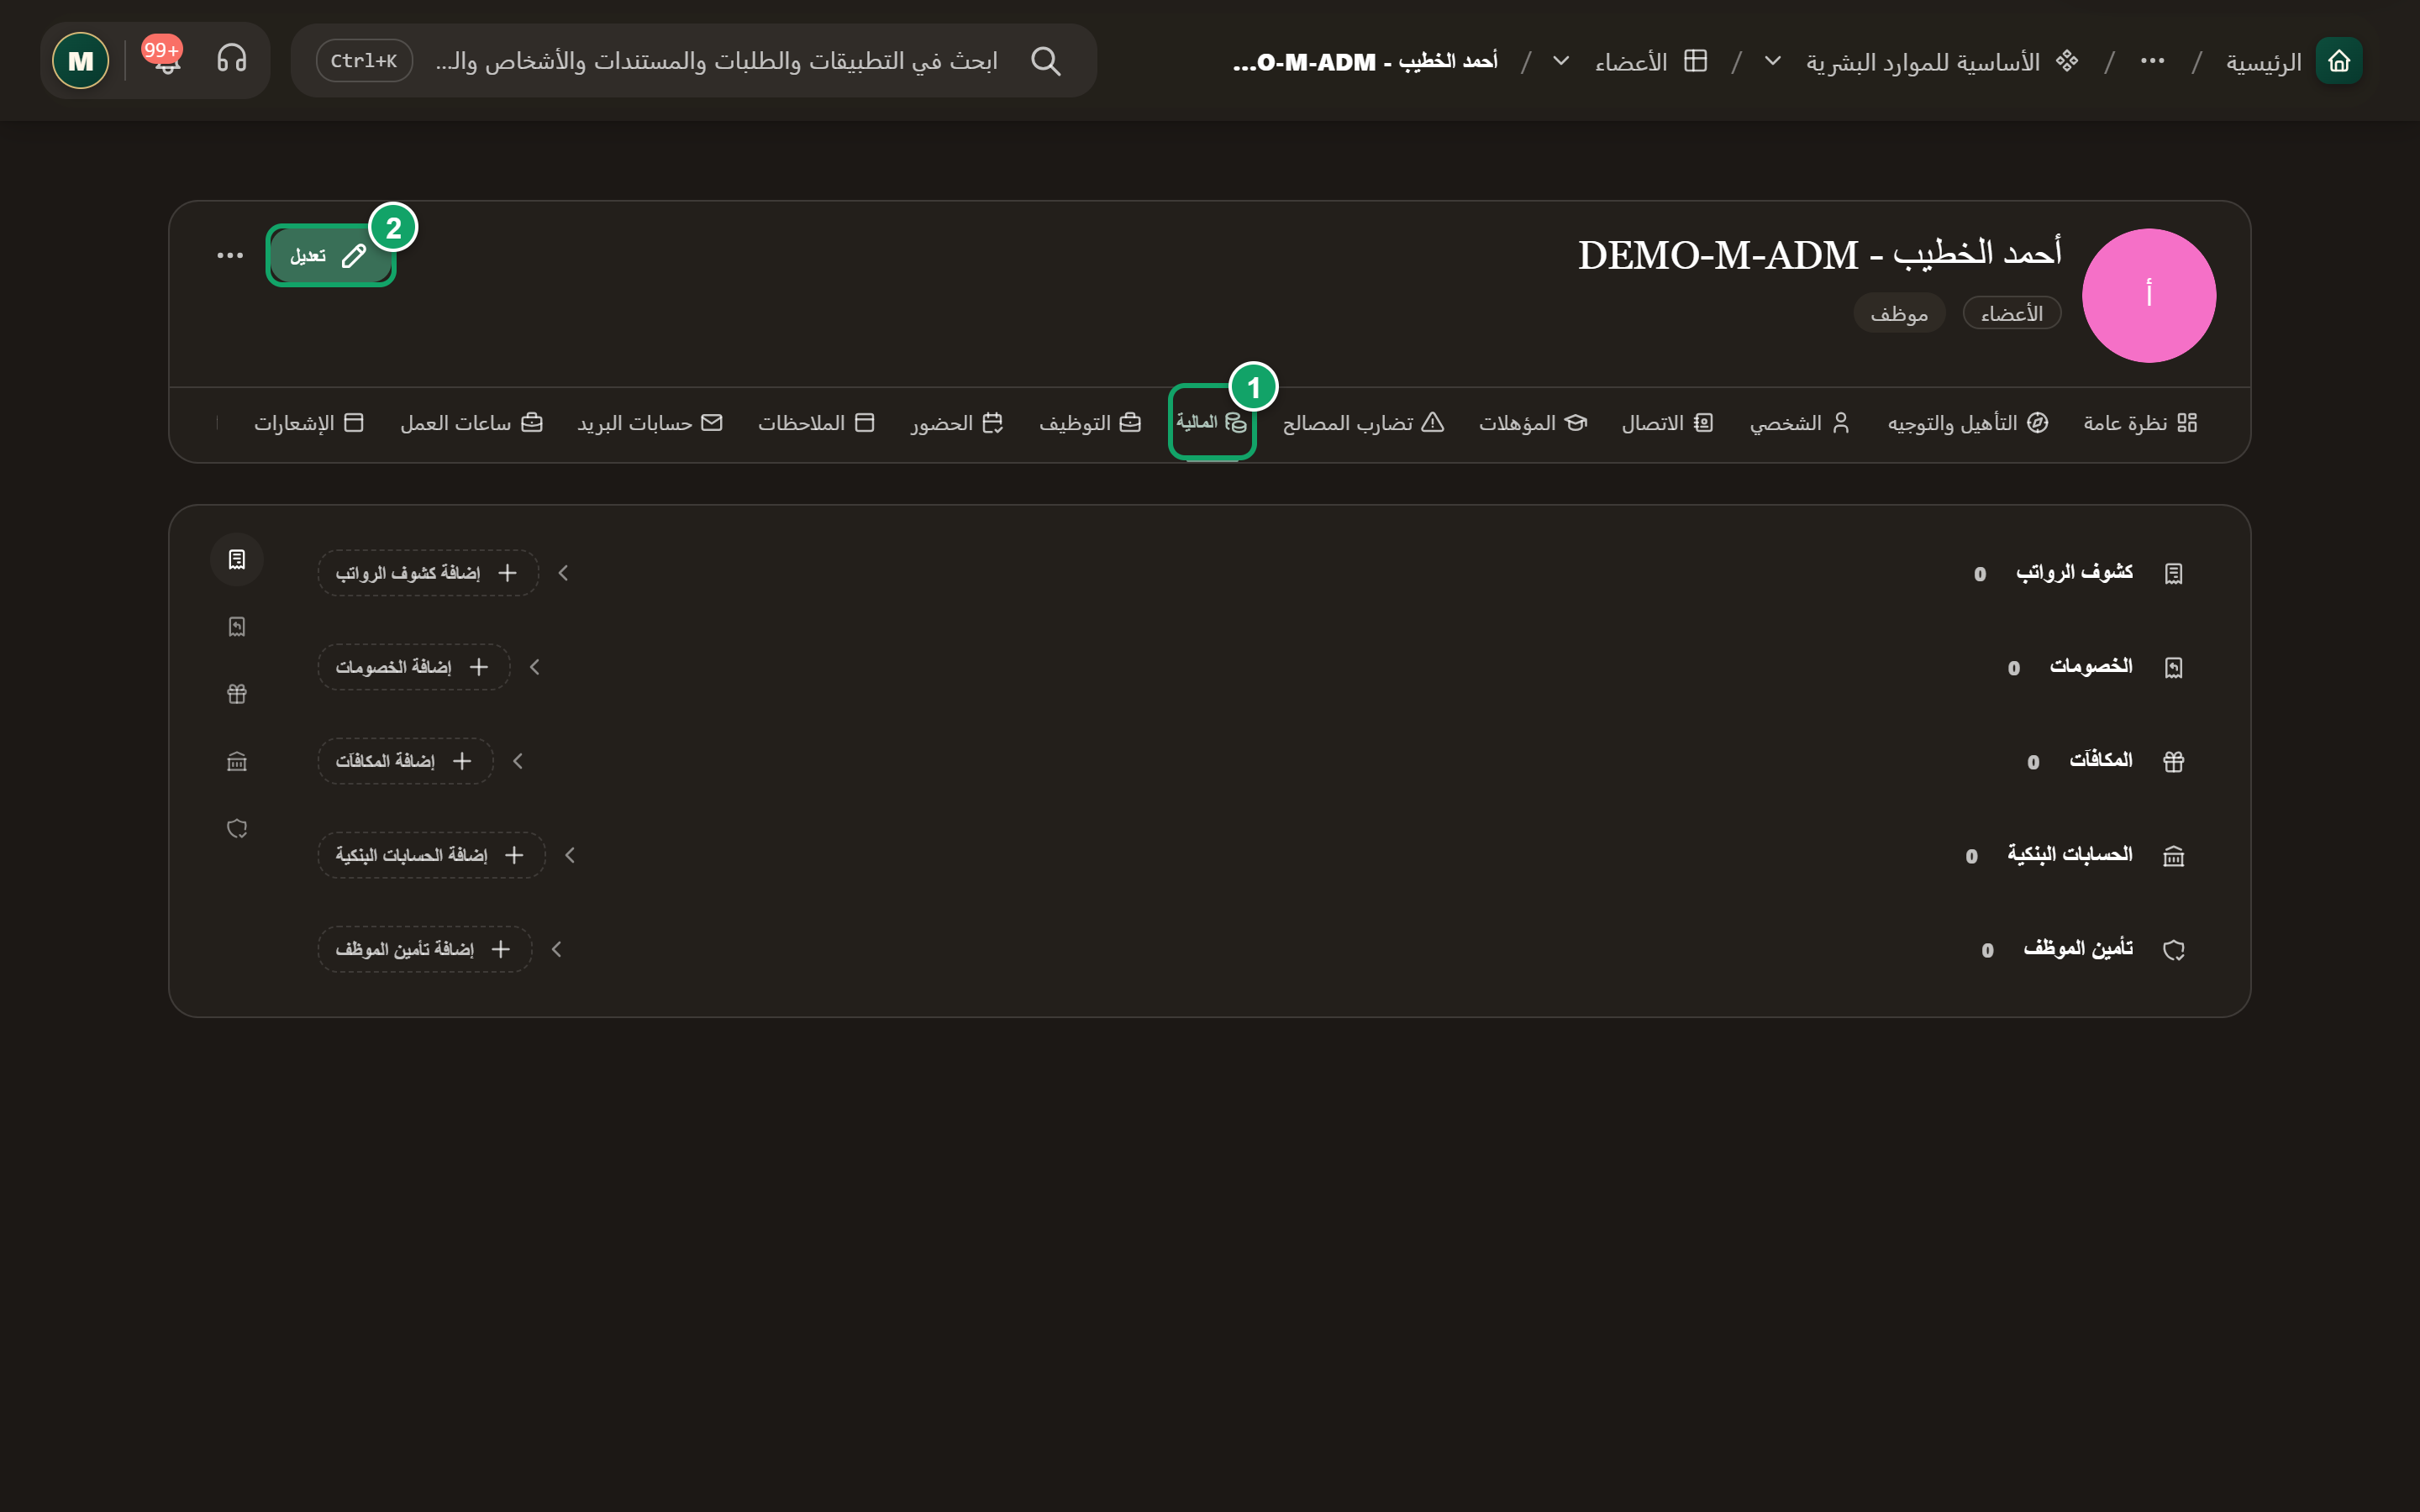
\includegraphics[width=0.95\linewidth]{figures/screens/ch03-member-tab7-ar.png}
\caption{ملف الموظف التجريبي — تبويب «المالية»}
\label{fig:hr-member-tab7}
\end{figure}

\begin{figure}[H]
\centering
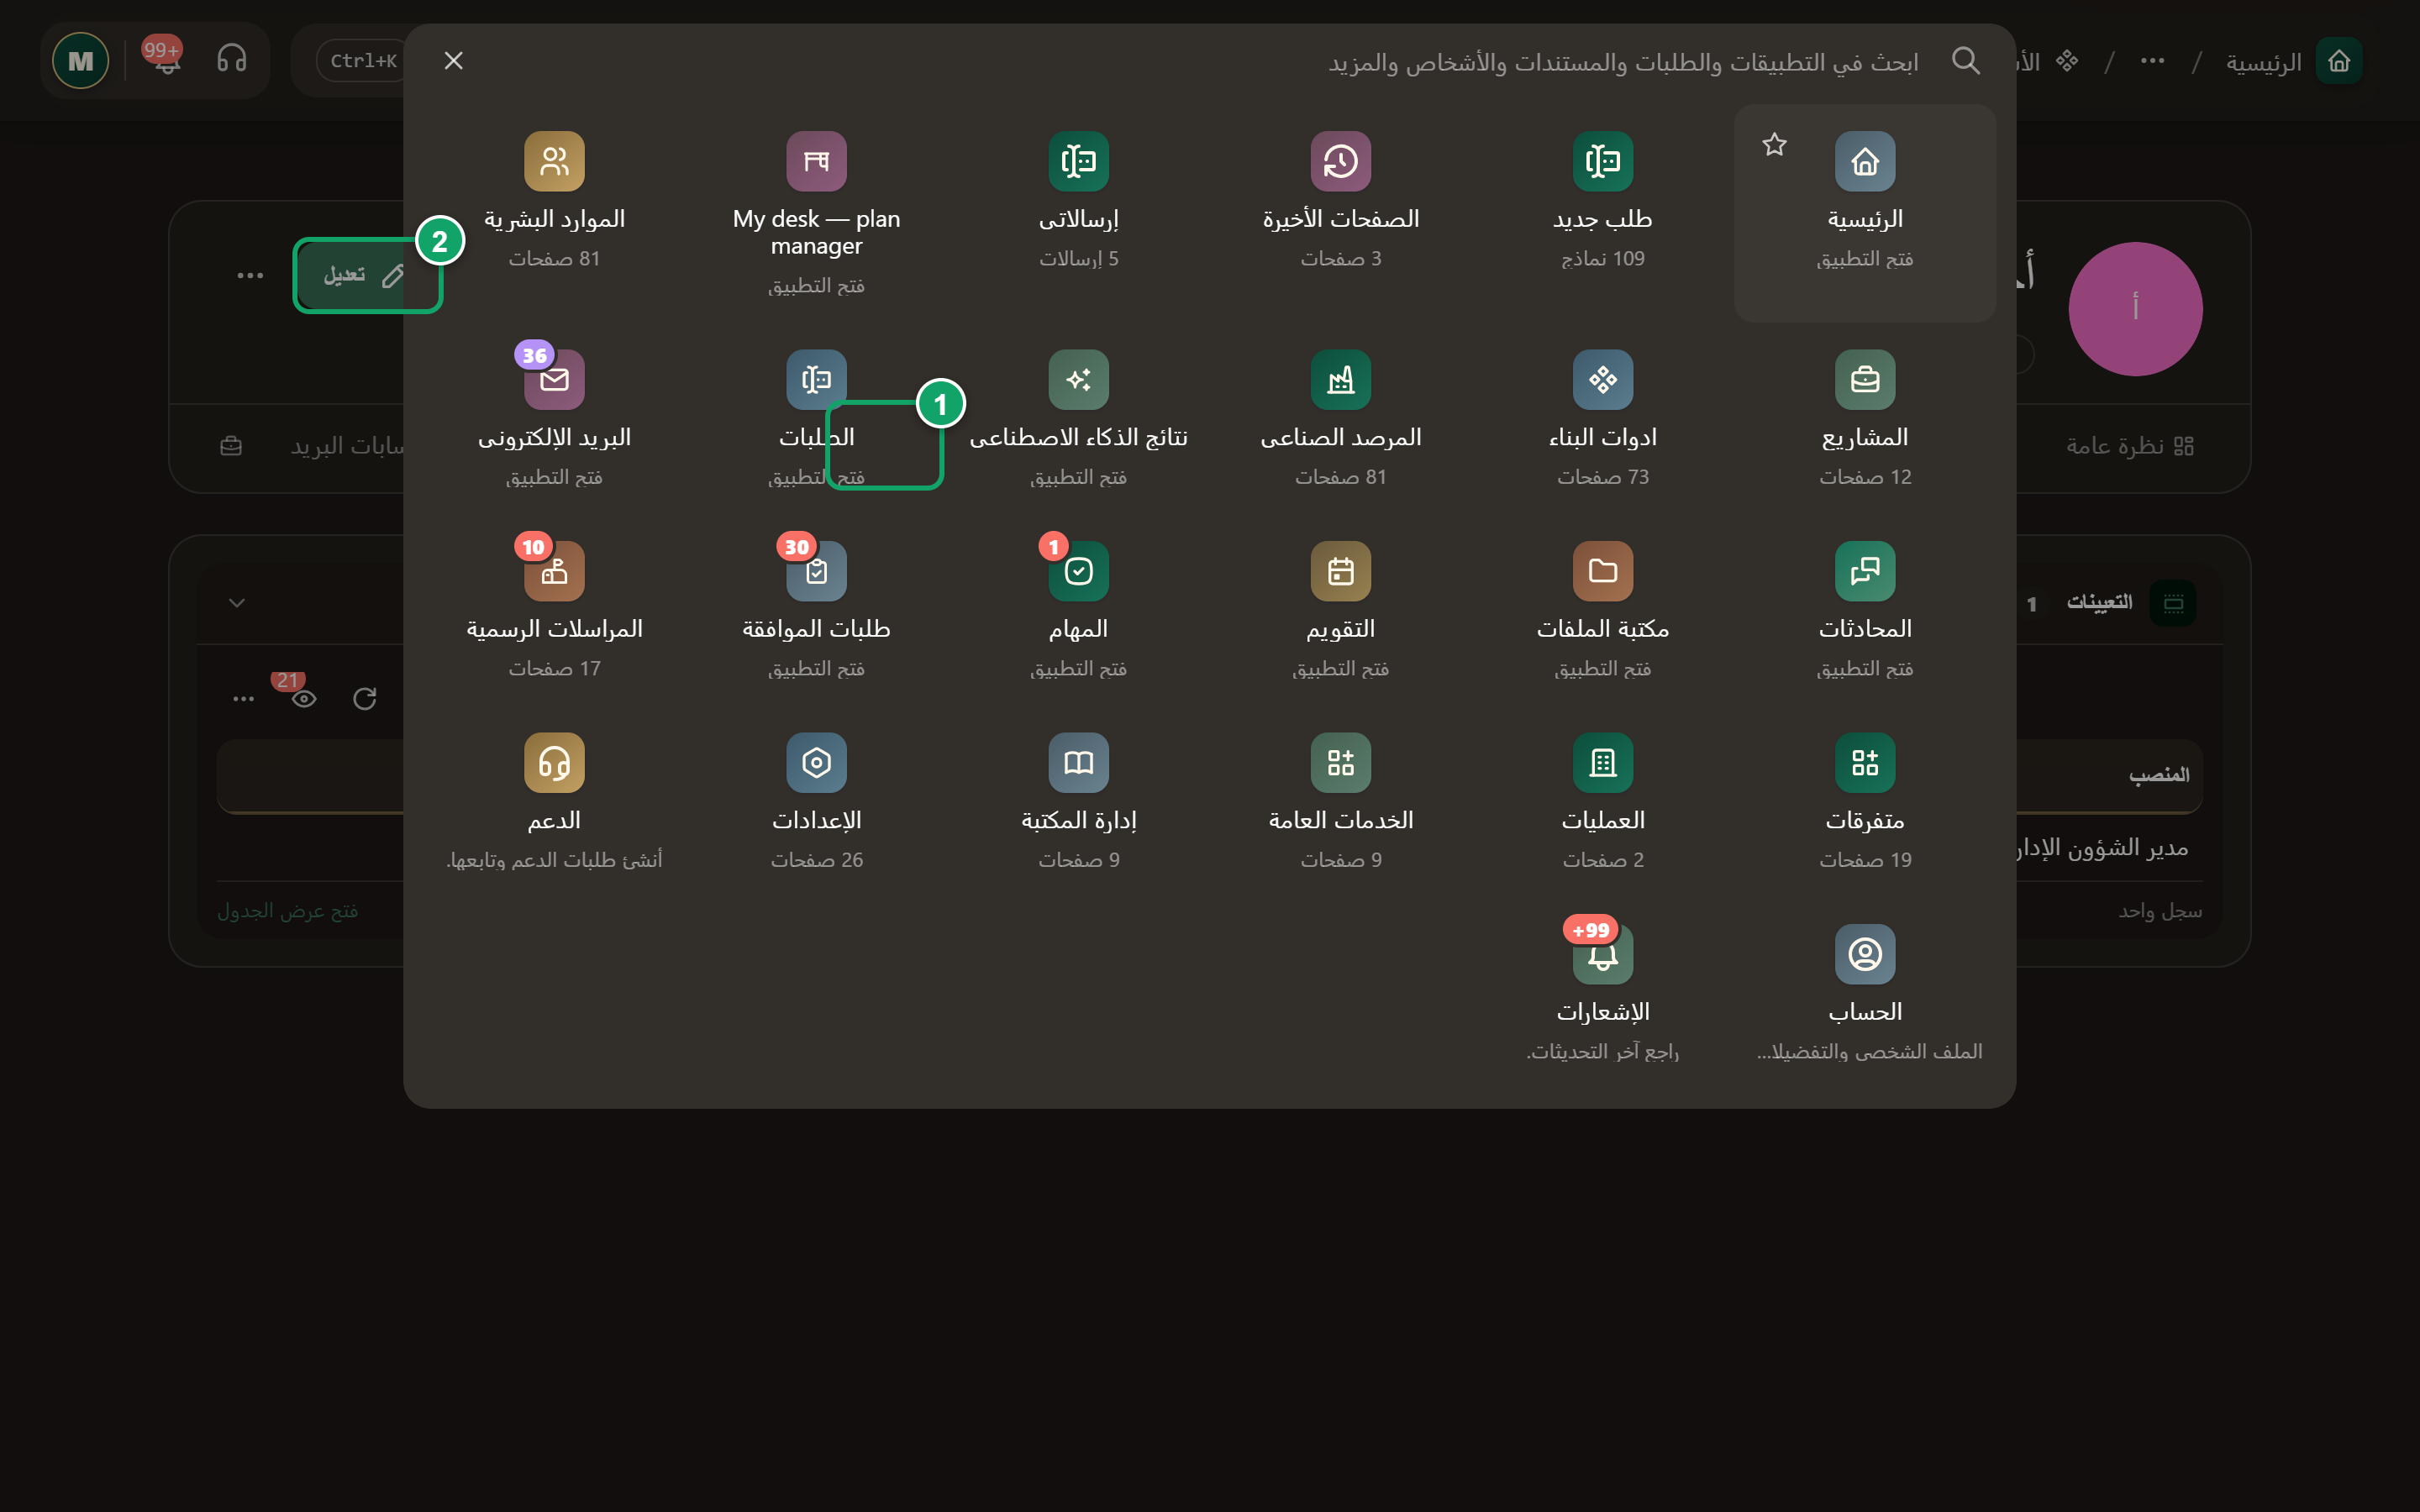
\includegraphics[width=0.95\linewidth]{figures/screens/ch03-member-tab8-ar.png}
\caption{ملف الموظف التجريبي — تبويب «التوظيف»}
\label{fig:hr-member-tab8}
\end{figure}

\begin{figure}[H]
\centering
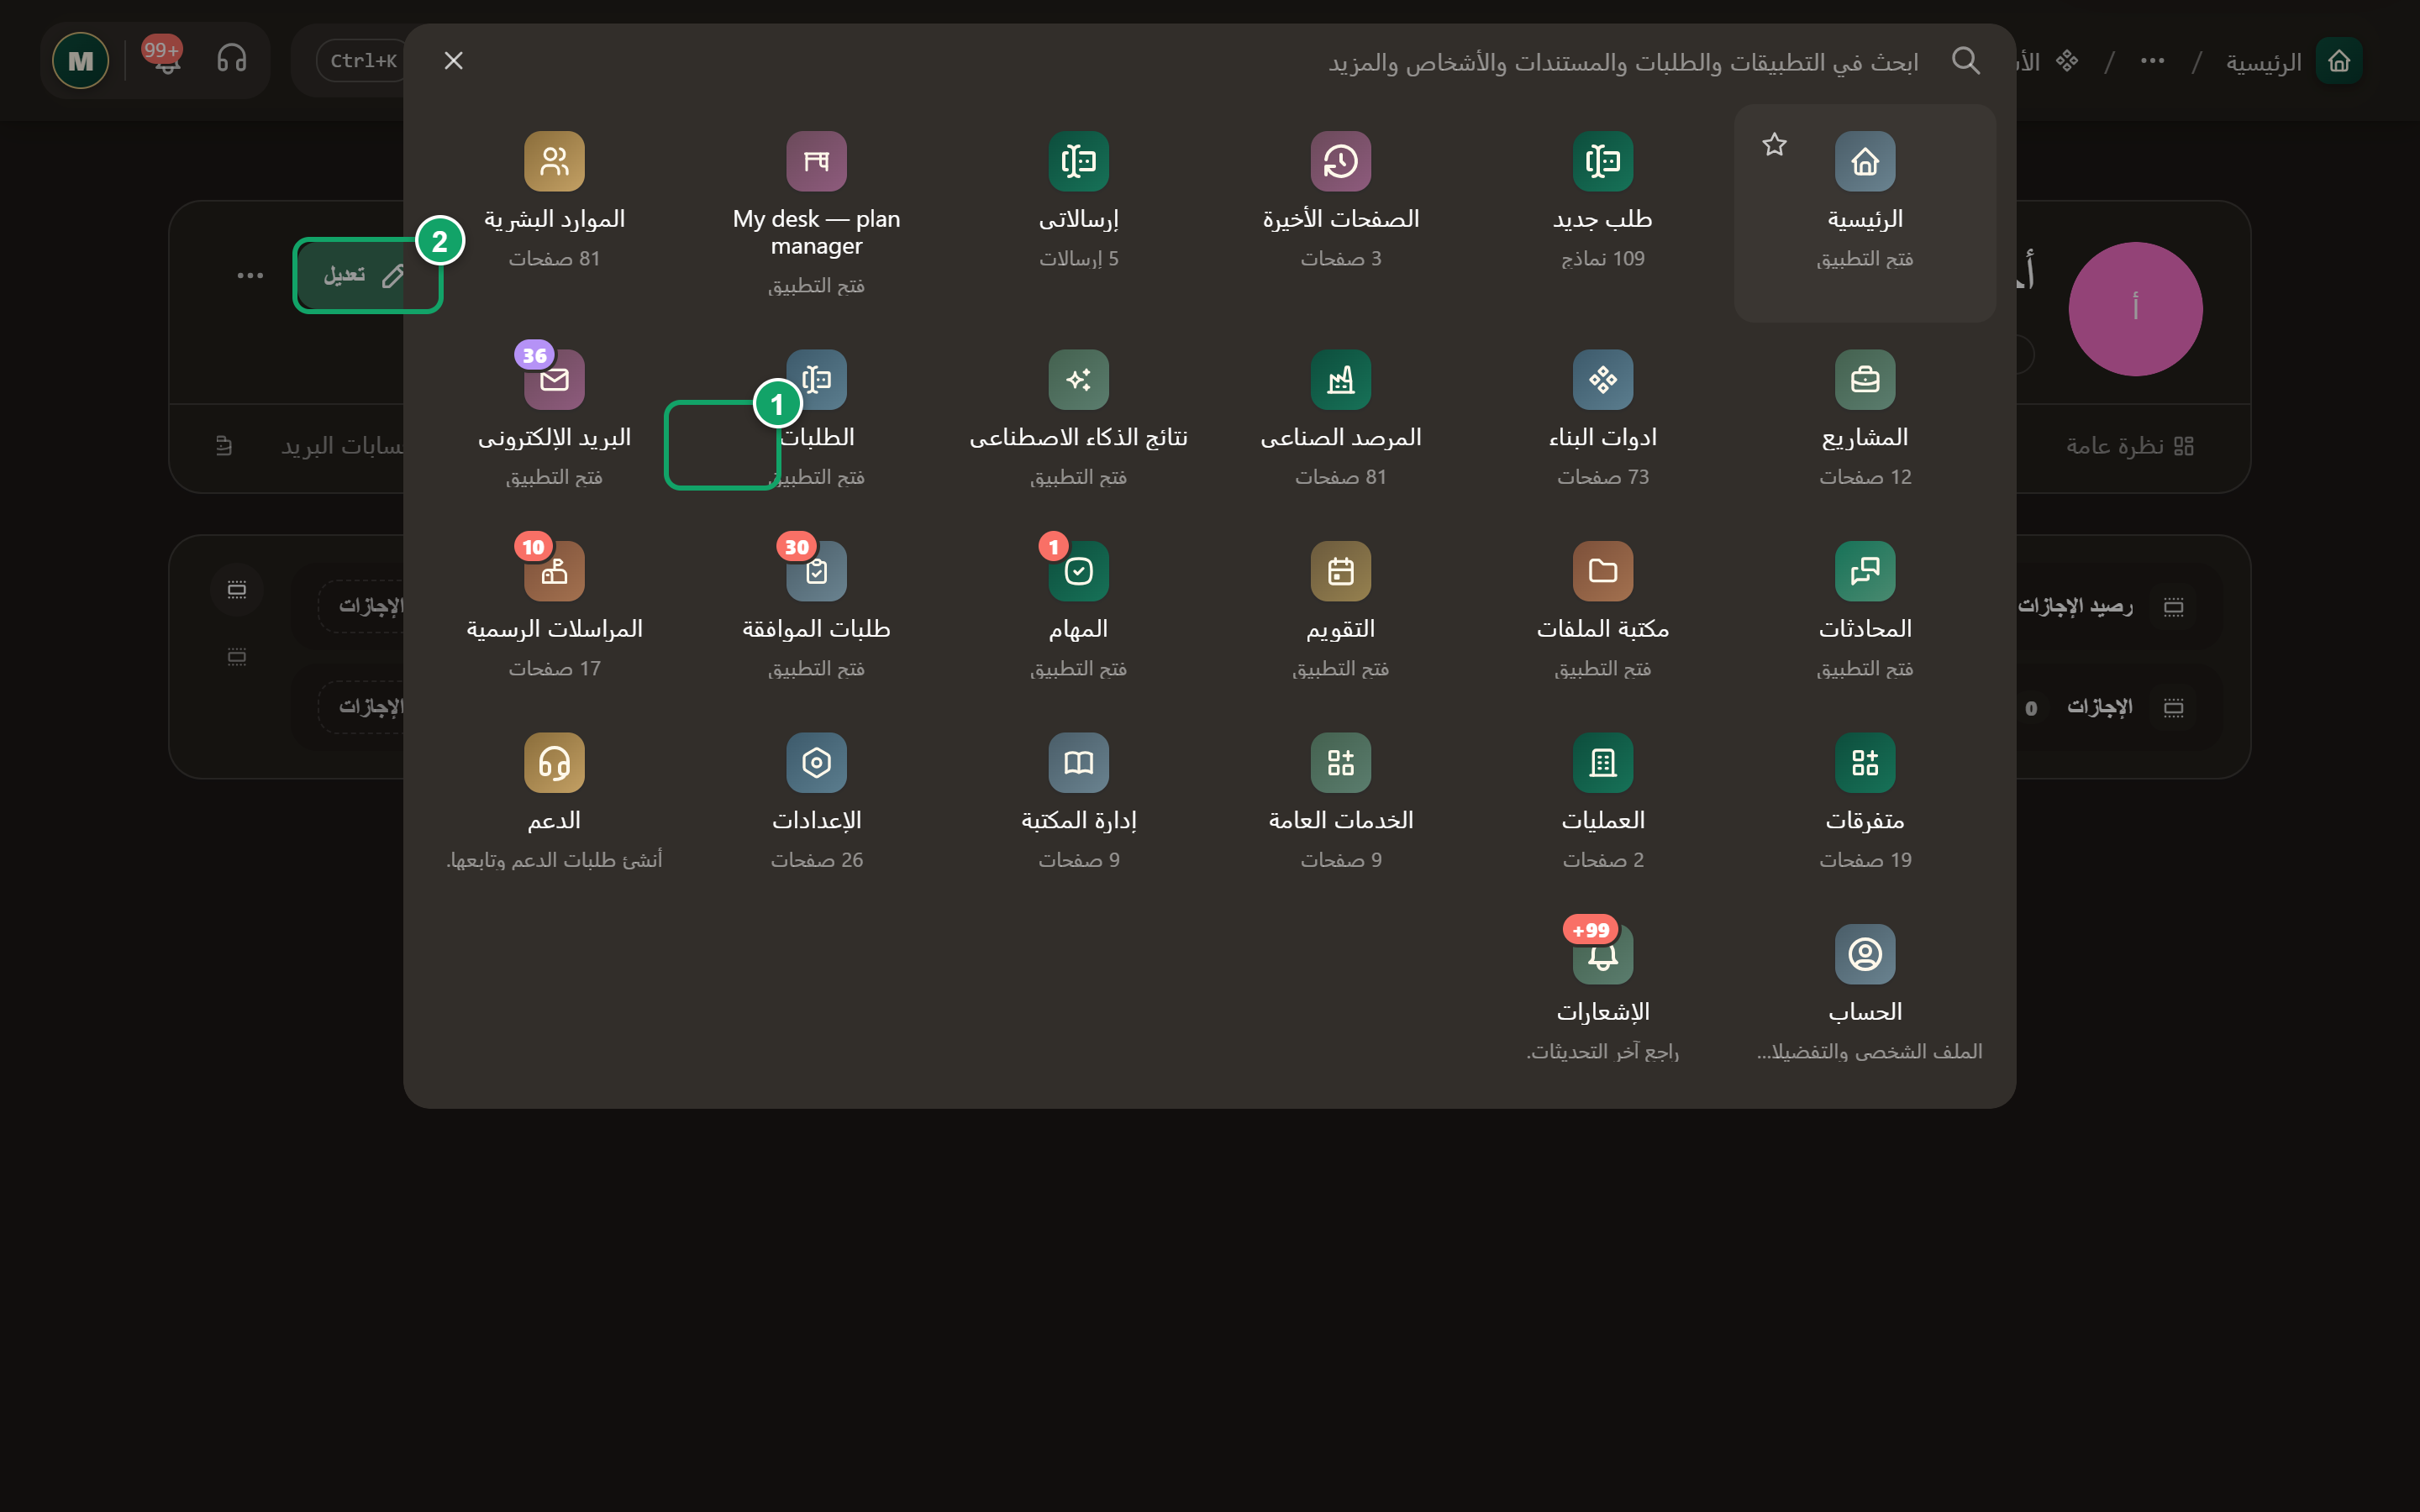
\includegraphics[width=0.95\linewidth]{figures/screens/ch03-member-tab9-ar.png}
\caption{ملف الموظف التجريبي — تبويب «الحضور»}
\label{fig:hr-member-tab9}
\end{figure}



\begin{figure}[H]
\centering
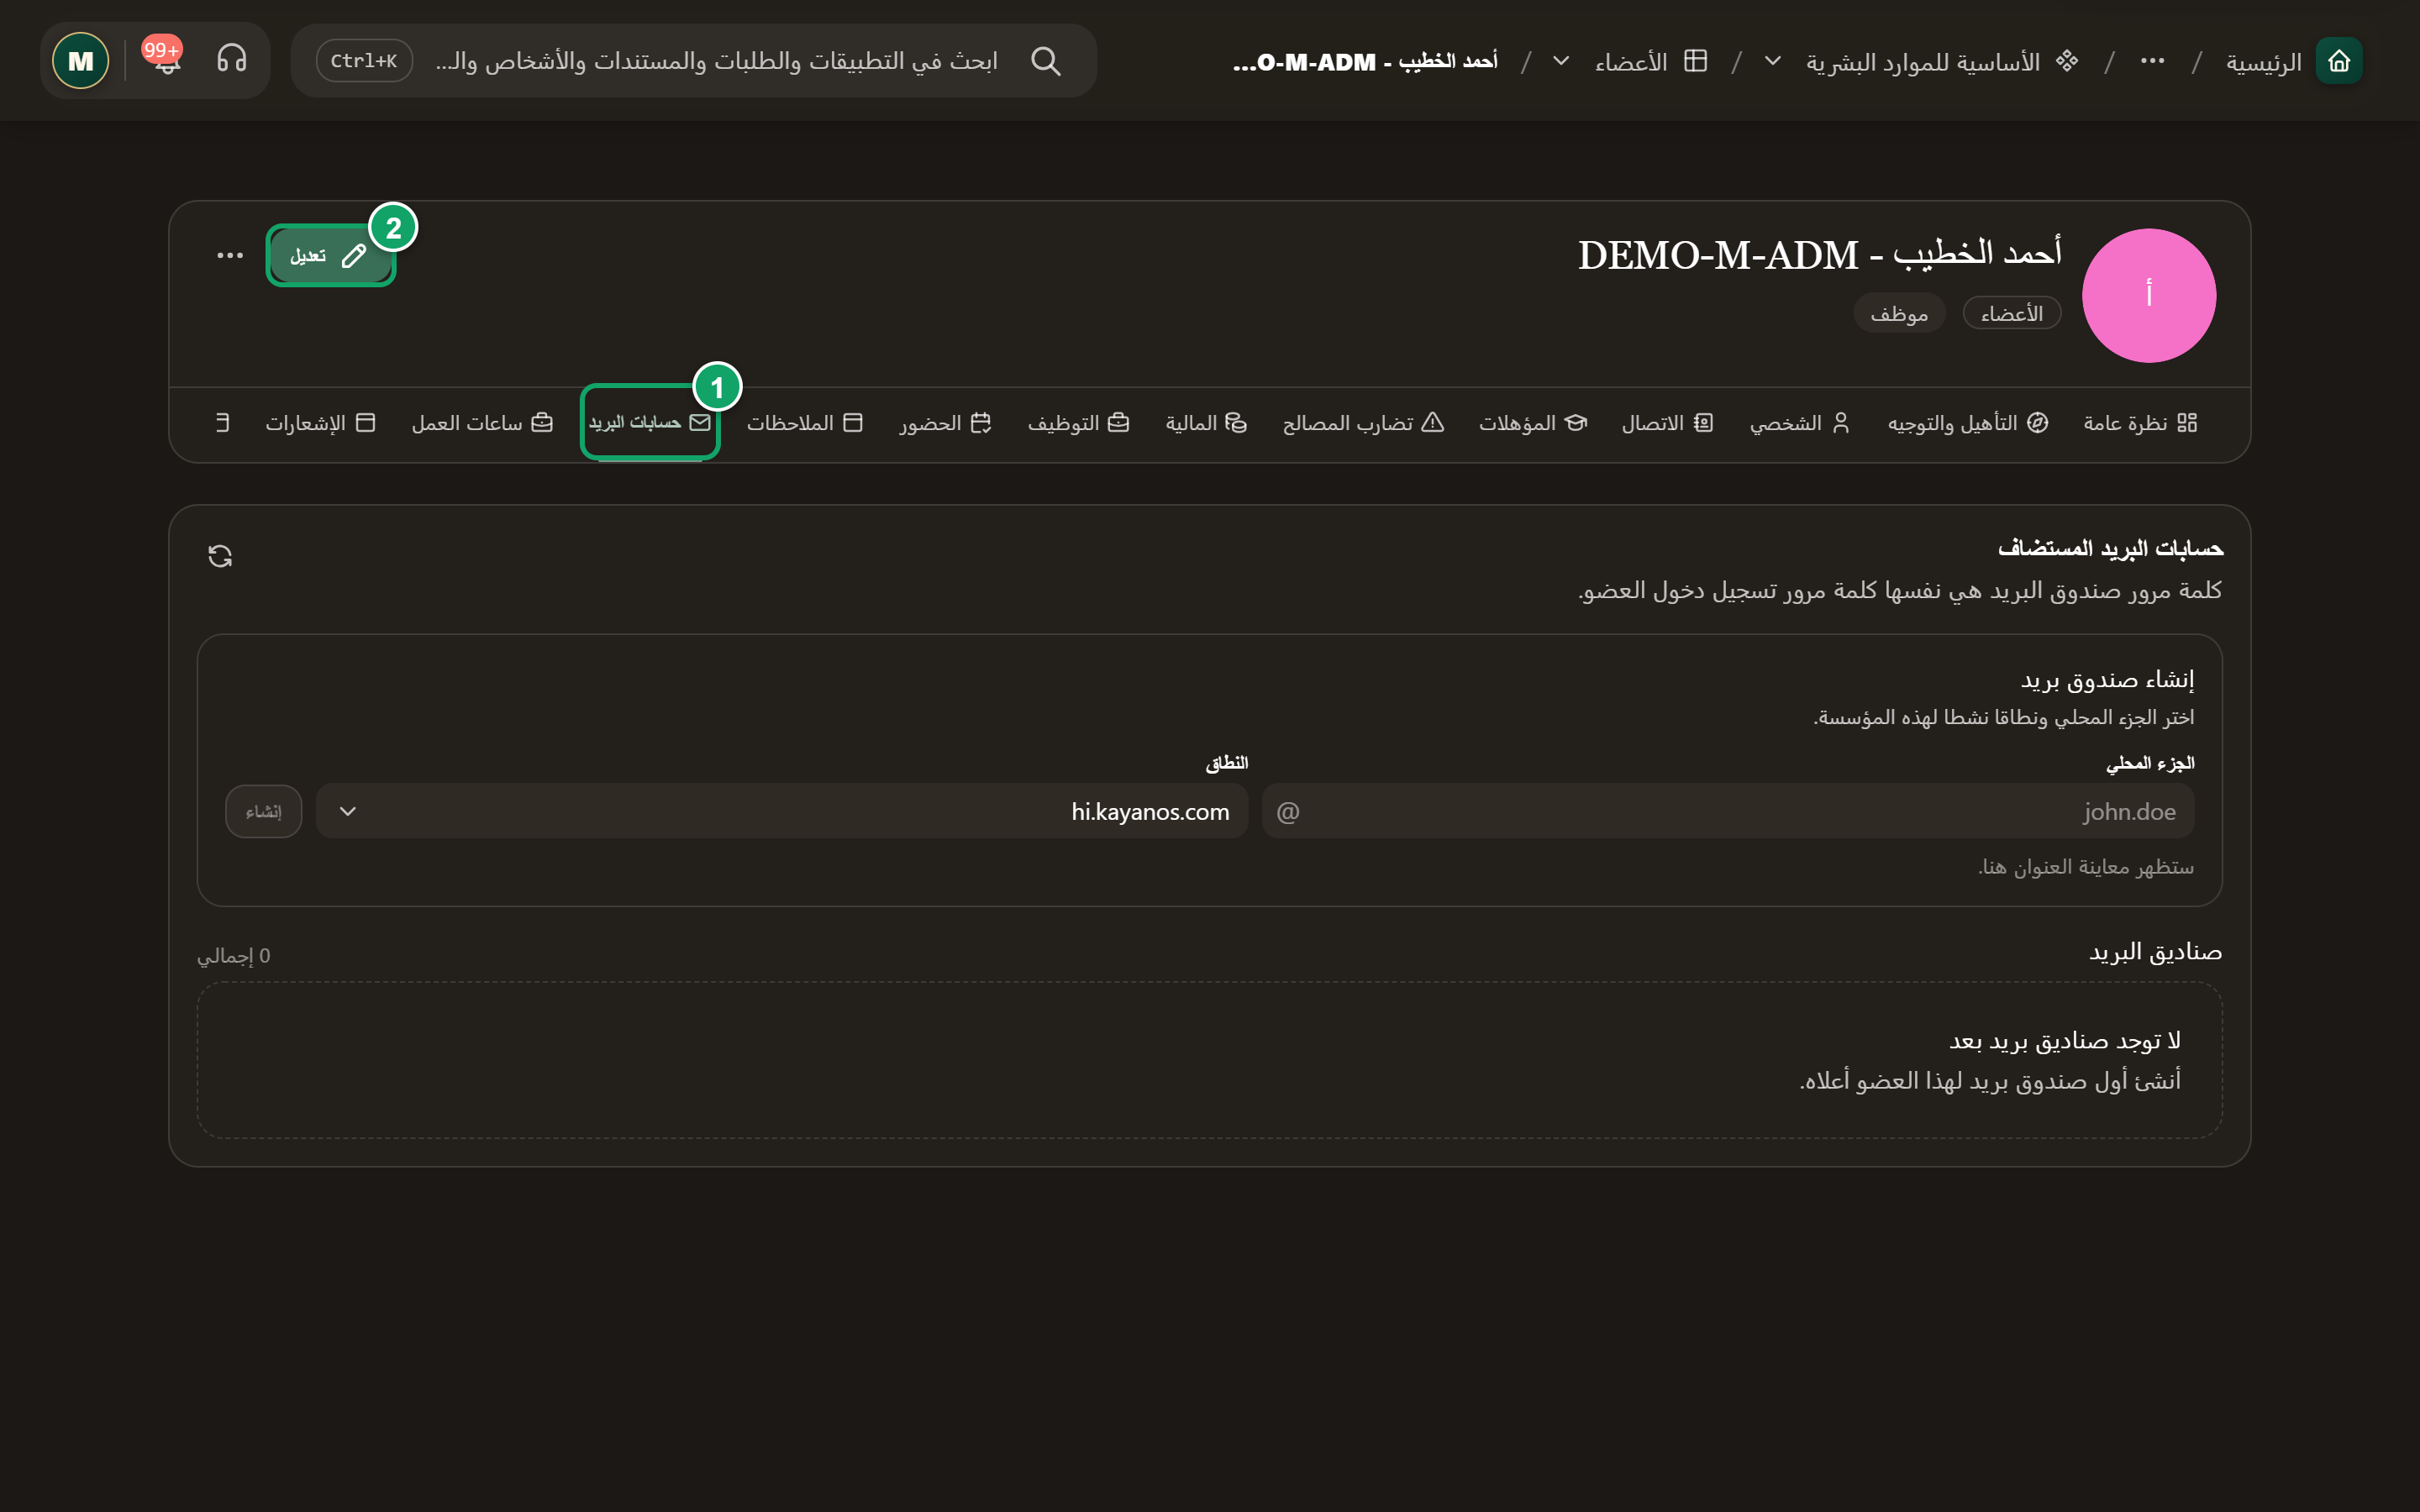
\includegraphics[width=0.95\linewidth]{figures/screens/ch03-member-tab11-ar.png}
\caption{ملف الموظف التجريبي — تبويب «حسابات البريد»}
\label{fig:hr-member-tab11}
\end{figure}

\begin{figure}[H]
\centering
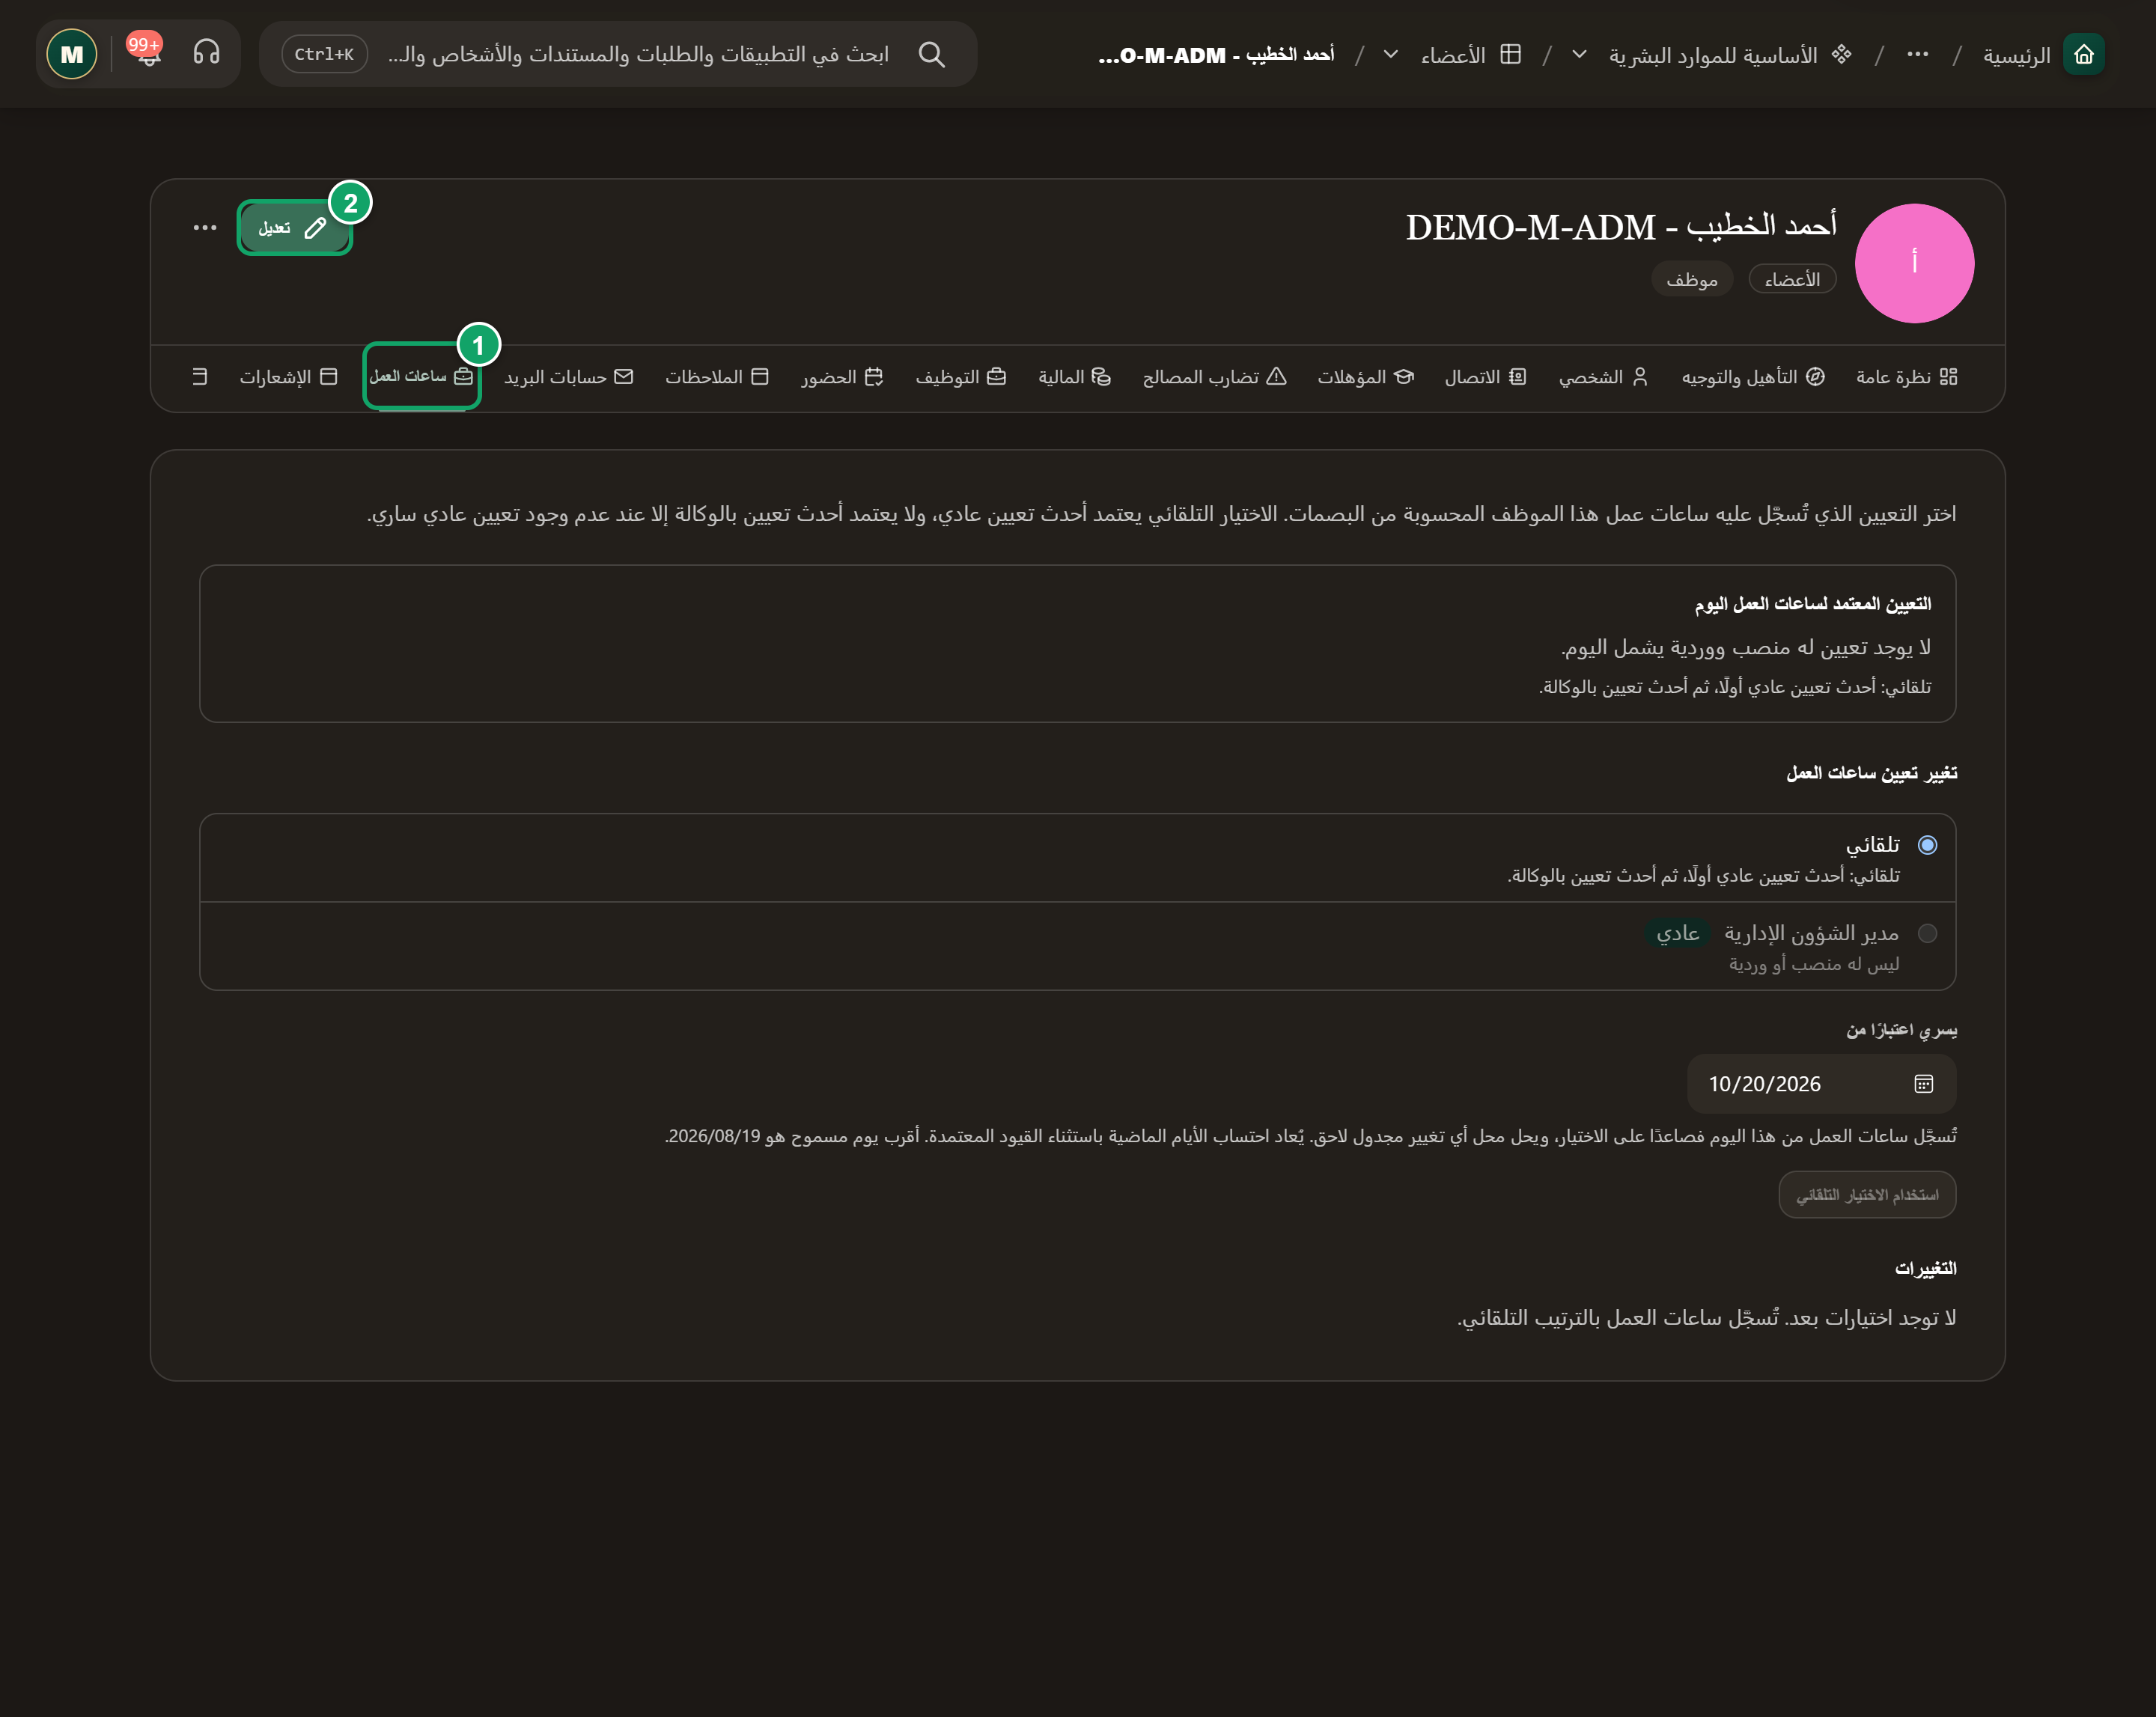
\includegraphics[width=0.95\linewidth]{figures/screens/ch03-member-tab12-ar.png}
\caption{ملف الموظف التجريبي — تبويب «ساعات العمل»}
\label{fig:hr-member-tab12}
\end{figure}

\begin{figure}[H]
\centering
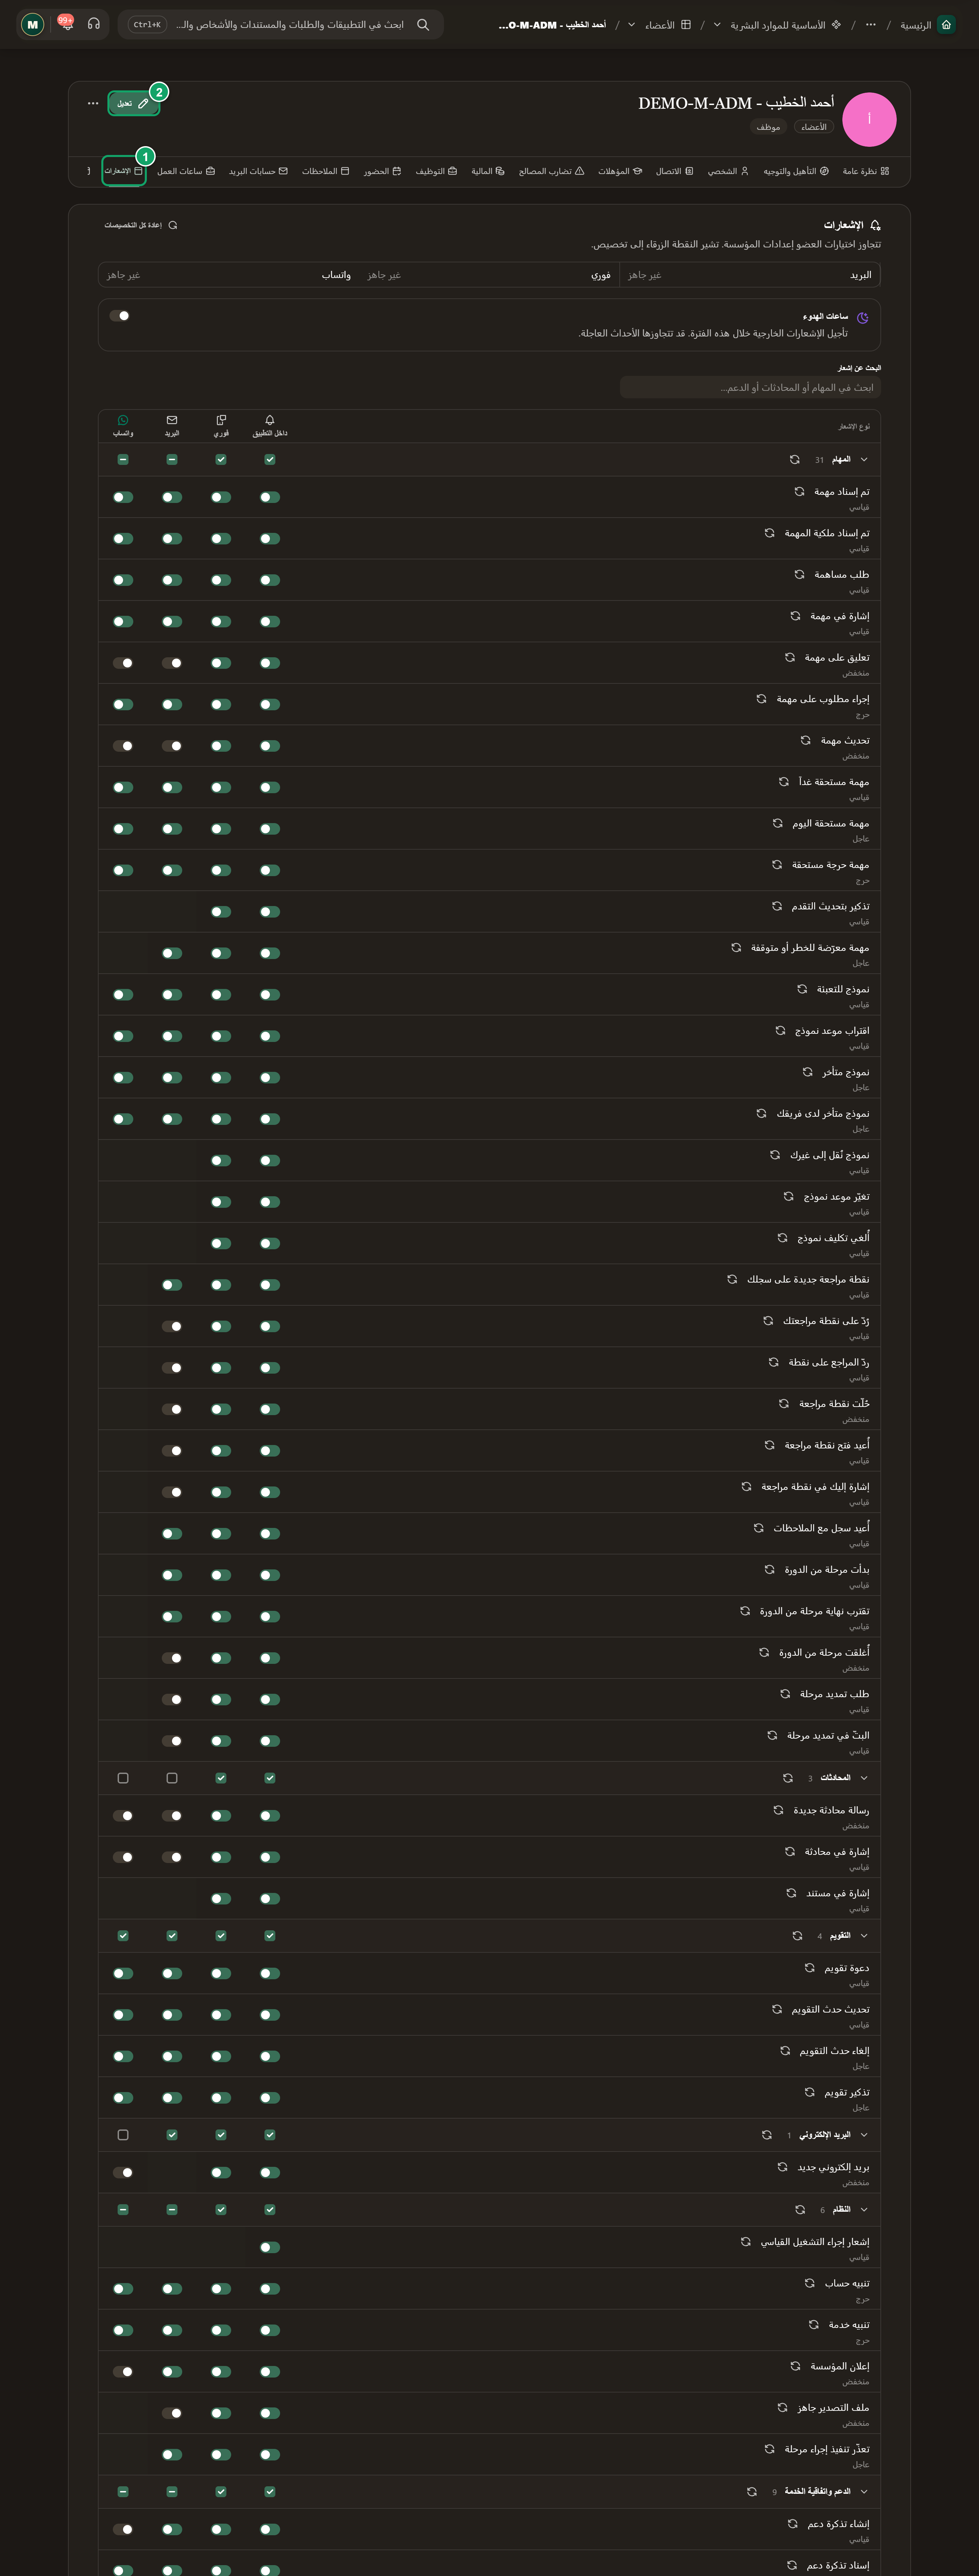
\includegraphics[width=0.95\linewidth]{figures/screens/ch03-member-tab13-ar.png}
\caption{ملف الموظف التجريبي — تبويب «الإشعارات»}
\label{fig:hr-member-tab13}
\end{figure}

\begin{figure}[H]
\centering
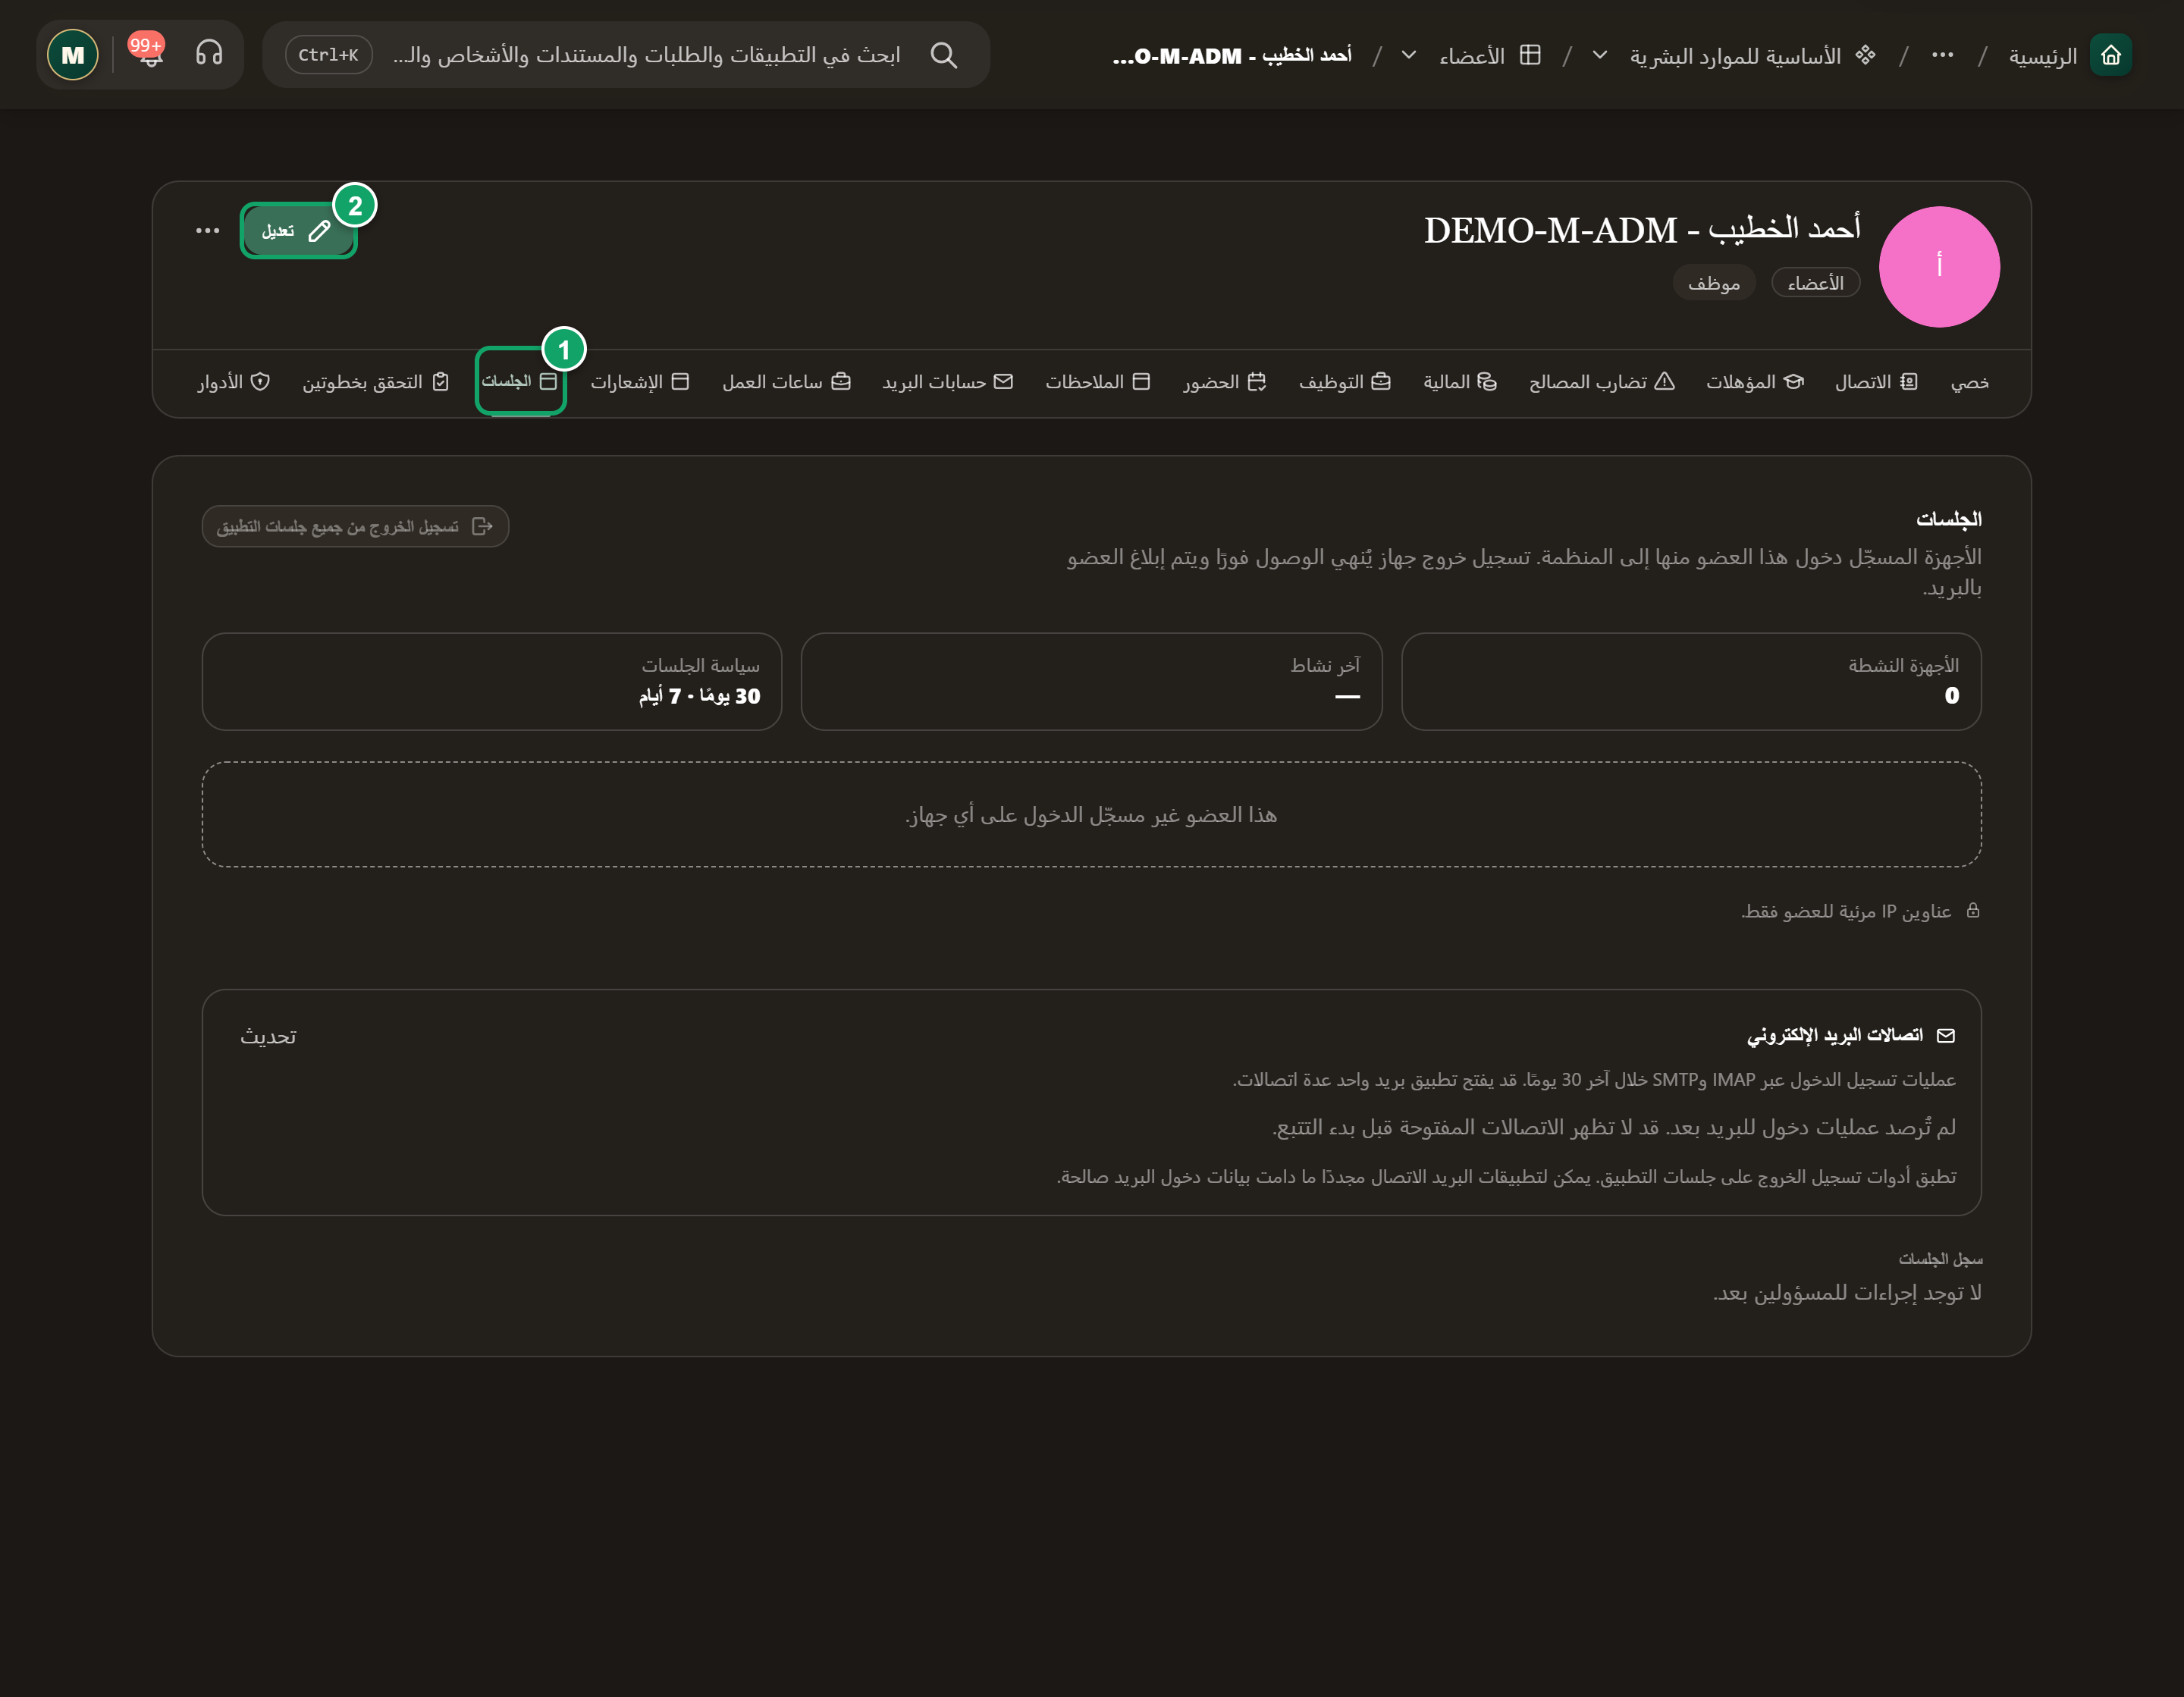
\includegraphics[width=0.95\linewidth]{figures/screens/ch03-member-tab14-ar.png}
\caption{ملف الموظف التجريبي — تبويب «الجلسات»}
\label{fig:hr-member-tab14}
\end{figure}

\begin{figure}[H]
\centering
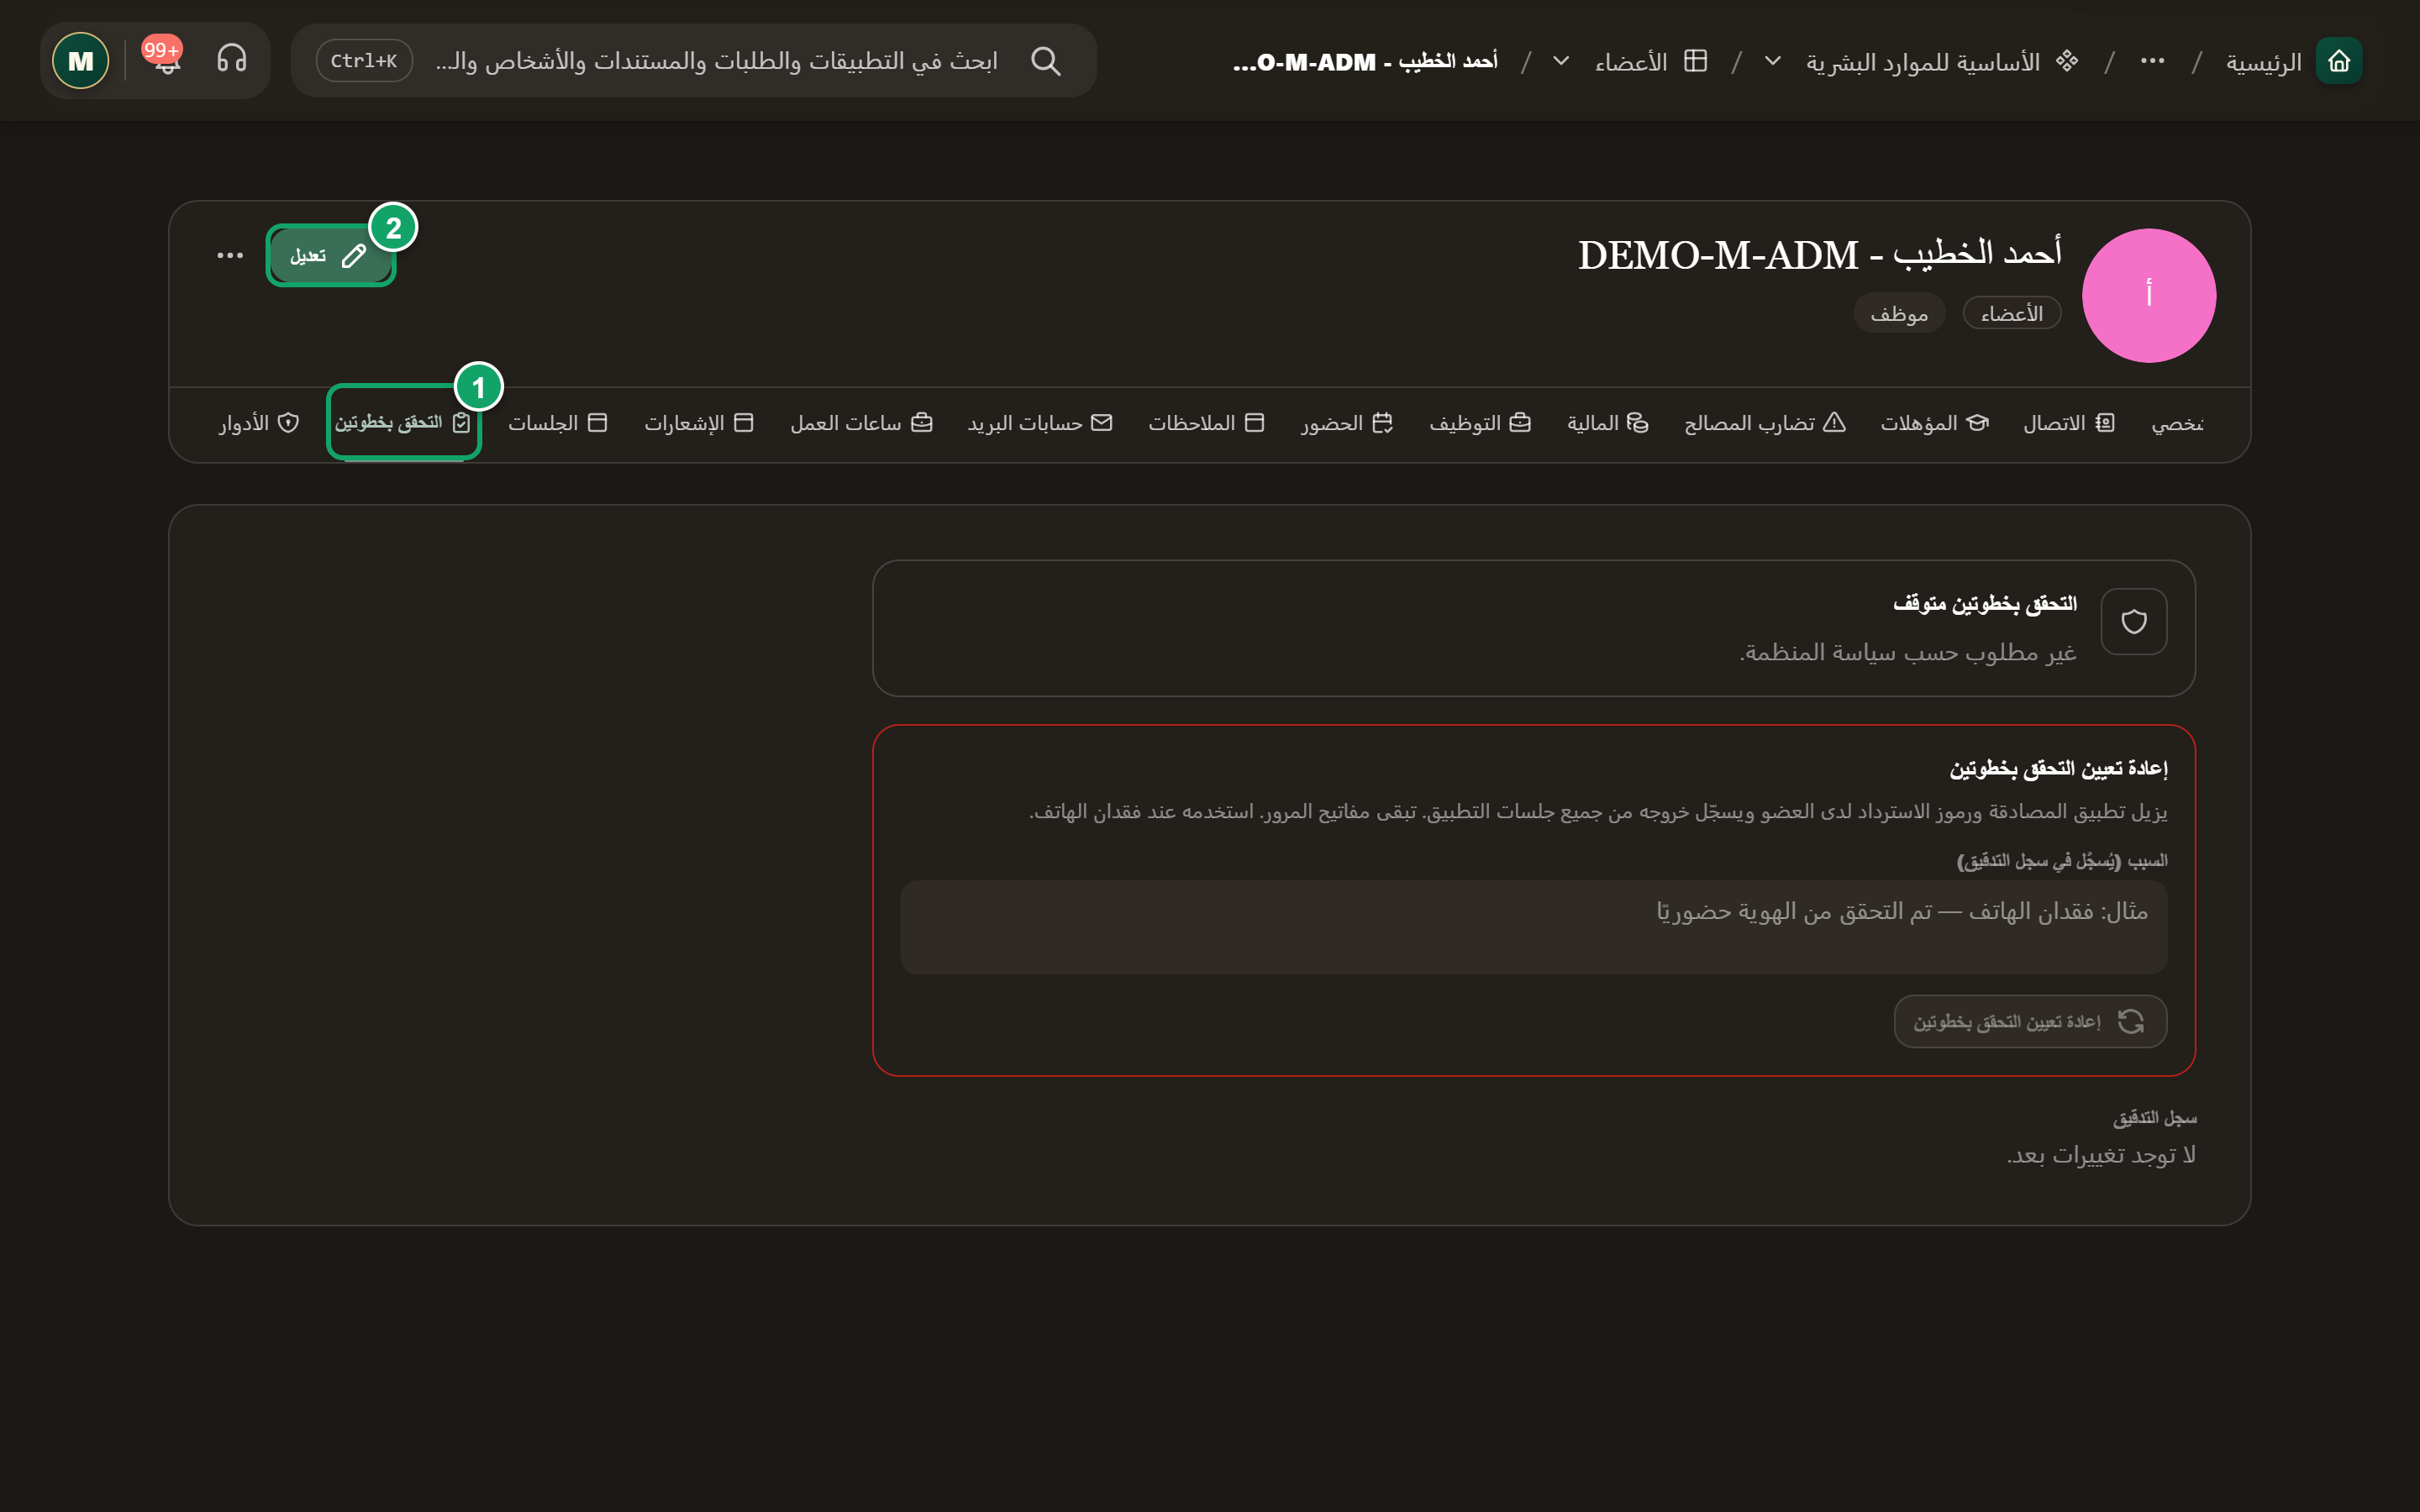
\includegraphics[width=0.95\linewidth]{figures/screens/ch03-member-tab15-ar.png}
\caption{ملف الموظف التجريبي — تبويب «التحقق بخطوتين»}
\label{fig:hr-member-tab15}
\end{figure}

\begin{figure}[H]
\centering
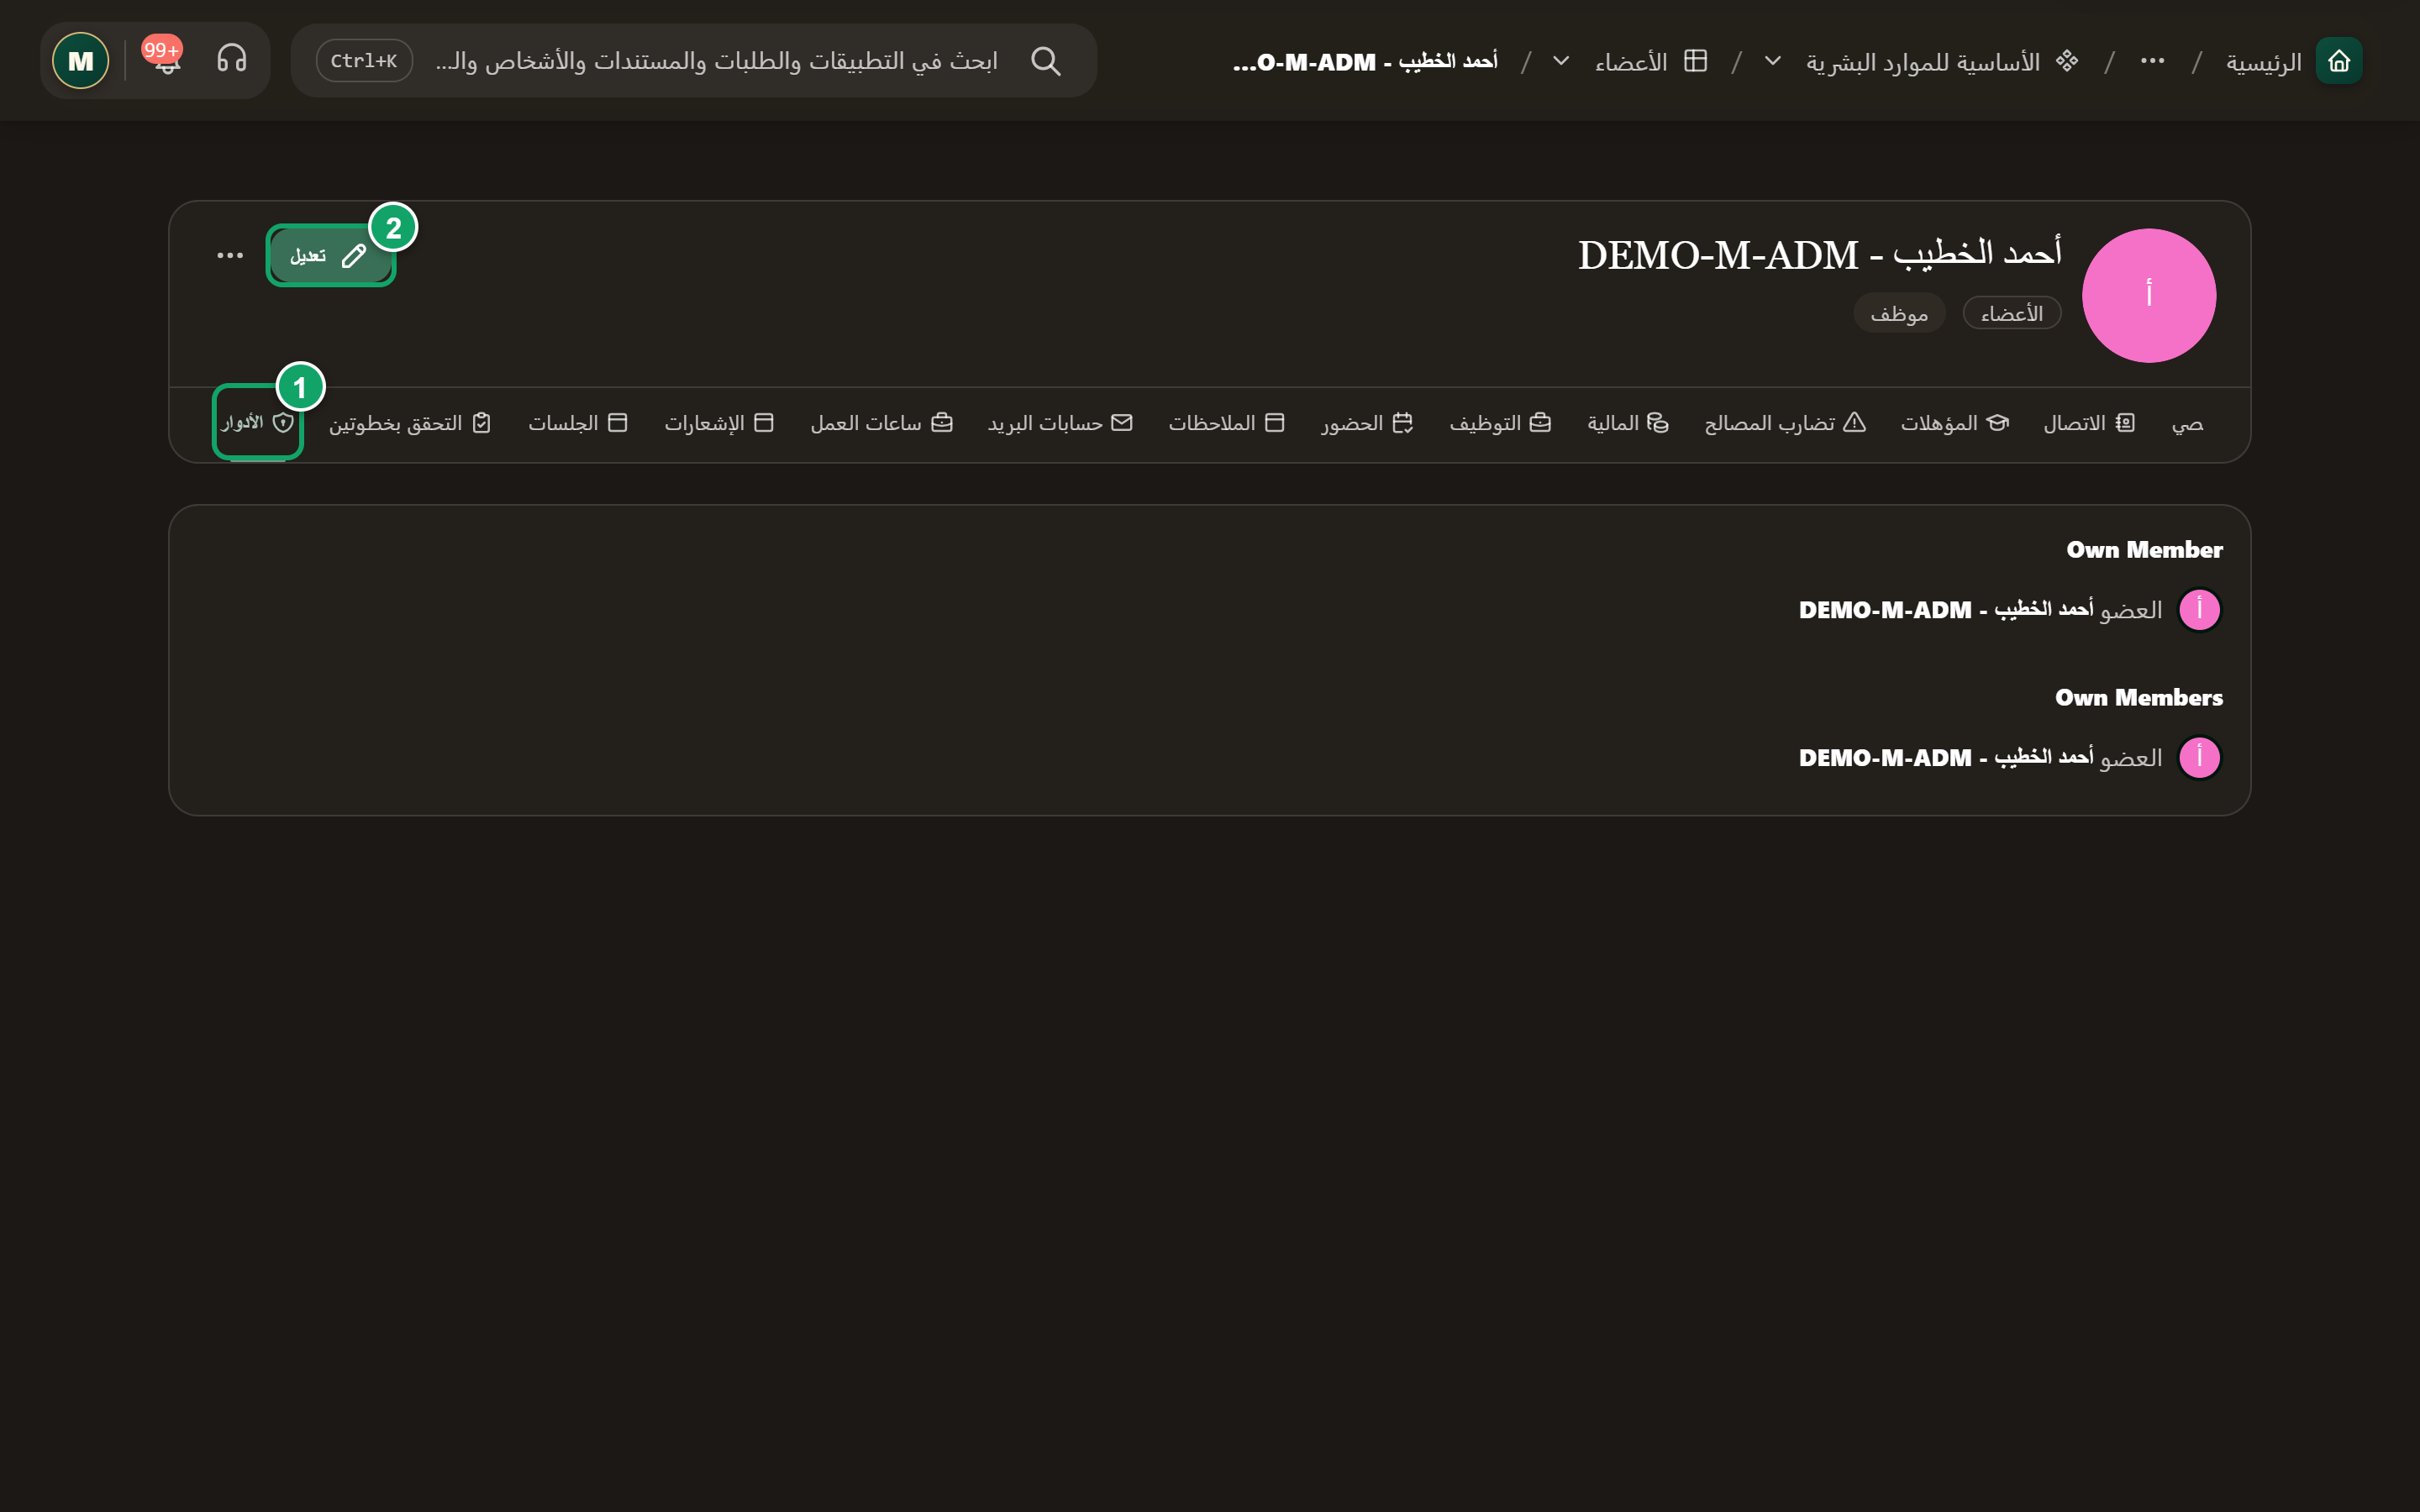
\includegraphics[width=0.95\linewidth]{figures/screens/ch03-member-tab16-ar.png}
\caption{ملف الموظف التجريبي — تبويب «الأدوار»}
\label{fig:hr-member-tab16}
\end{figure}

\clearpage
\section{المناصب}
\label{sec:hr-feature-positions}

المنصب وظيفة مثل مدير الموارد البشرية. تحدد فيه المنصب الذي يتبعه، وقسمه وموقعه ودرجته؛ ويحدد التعيين من يشغله.

\textbf{متى تفيد؟} عرّف الوظيفة مرة واحدة، ثم تابع من يشغلها، أو إن كانت شاغرة. \textbf{المسار:} «الموارد البشرية» / «القوى العاملة» / «المناصب».

\begin{figure}[H]
\centering
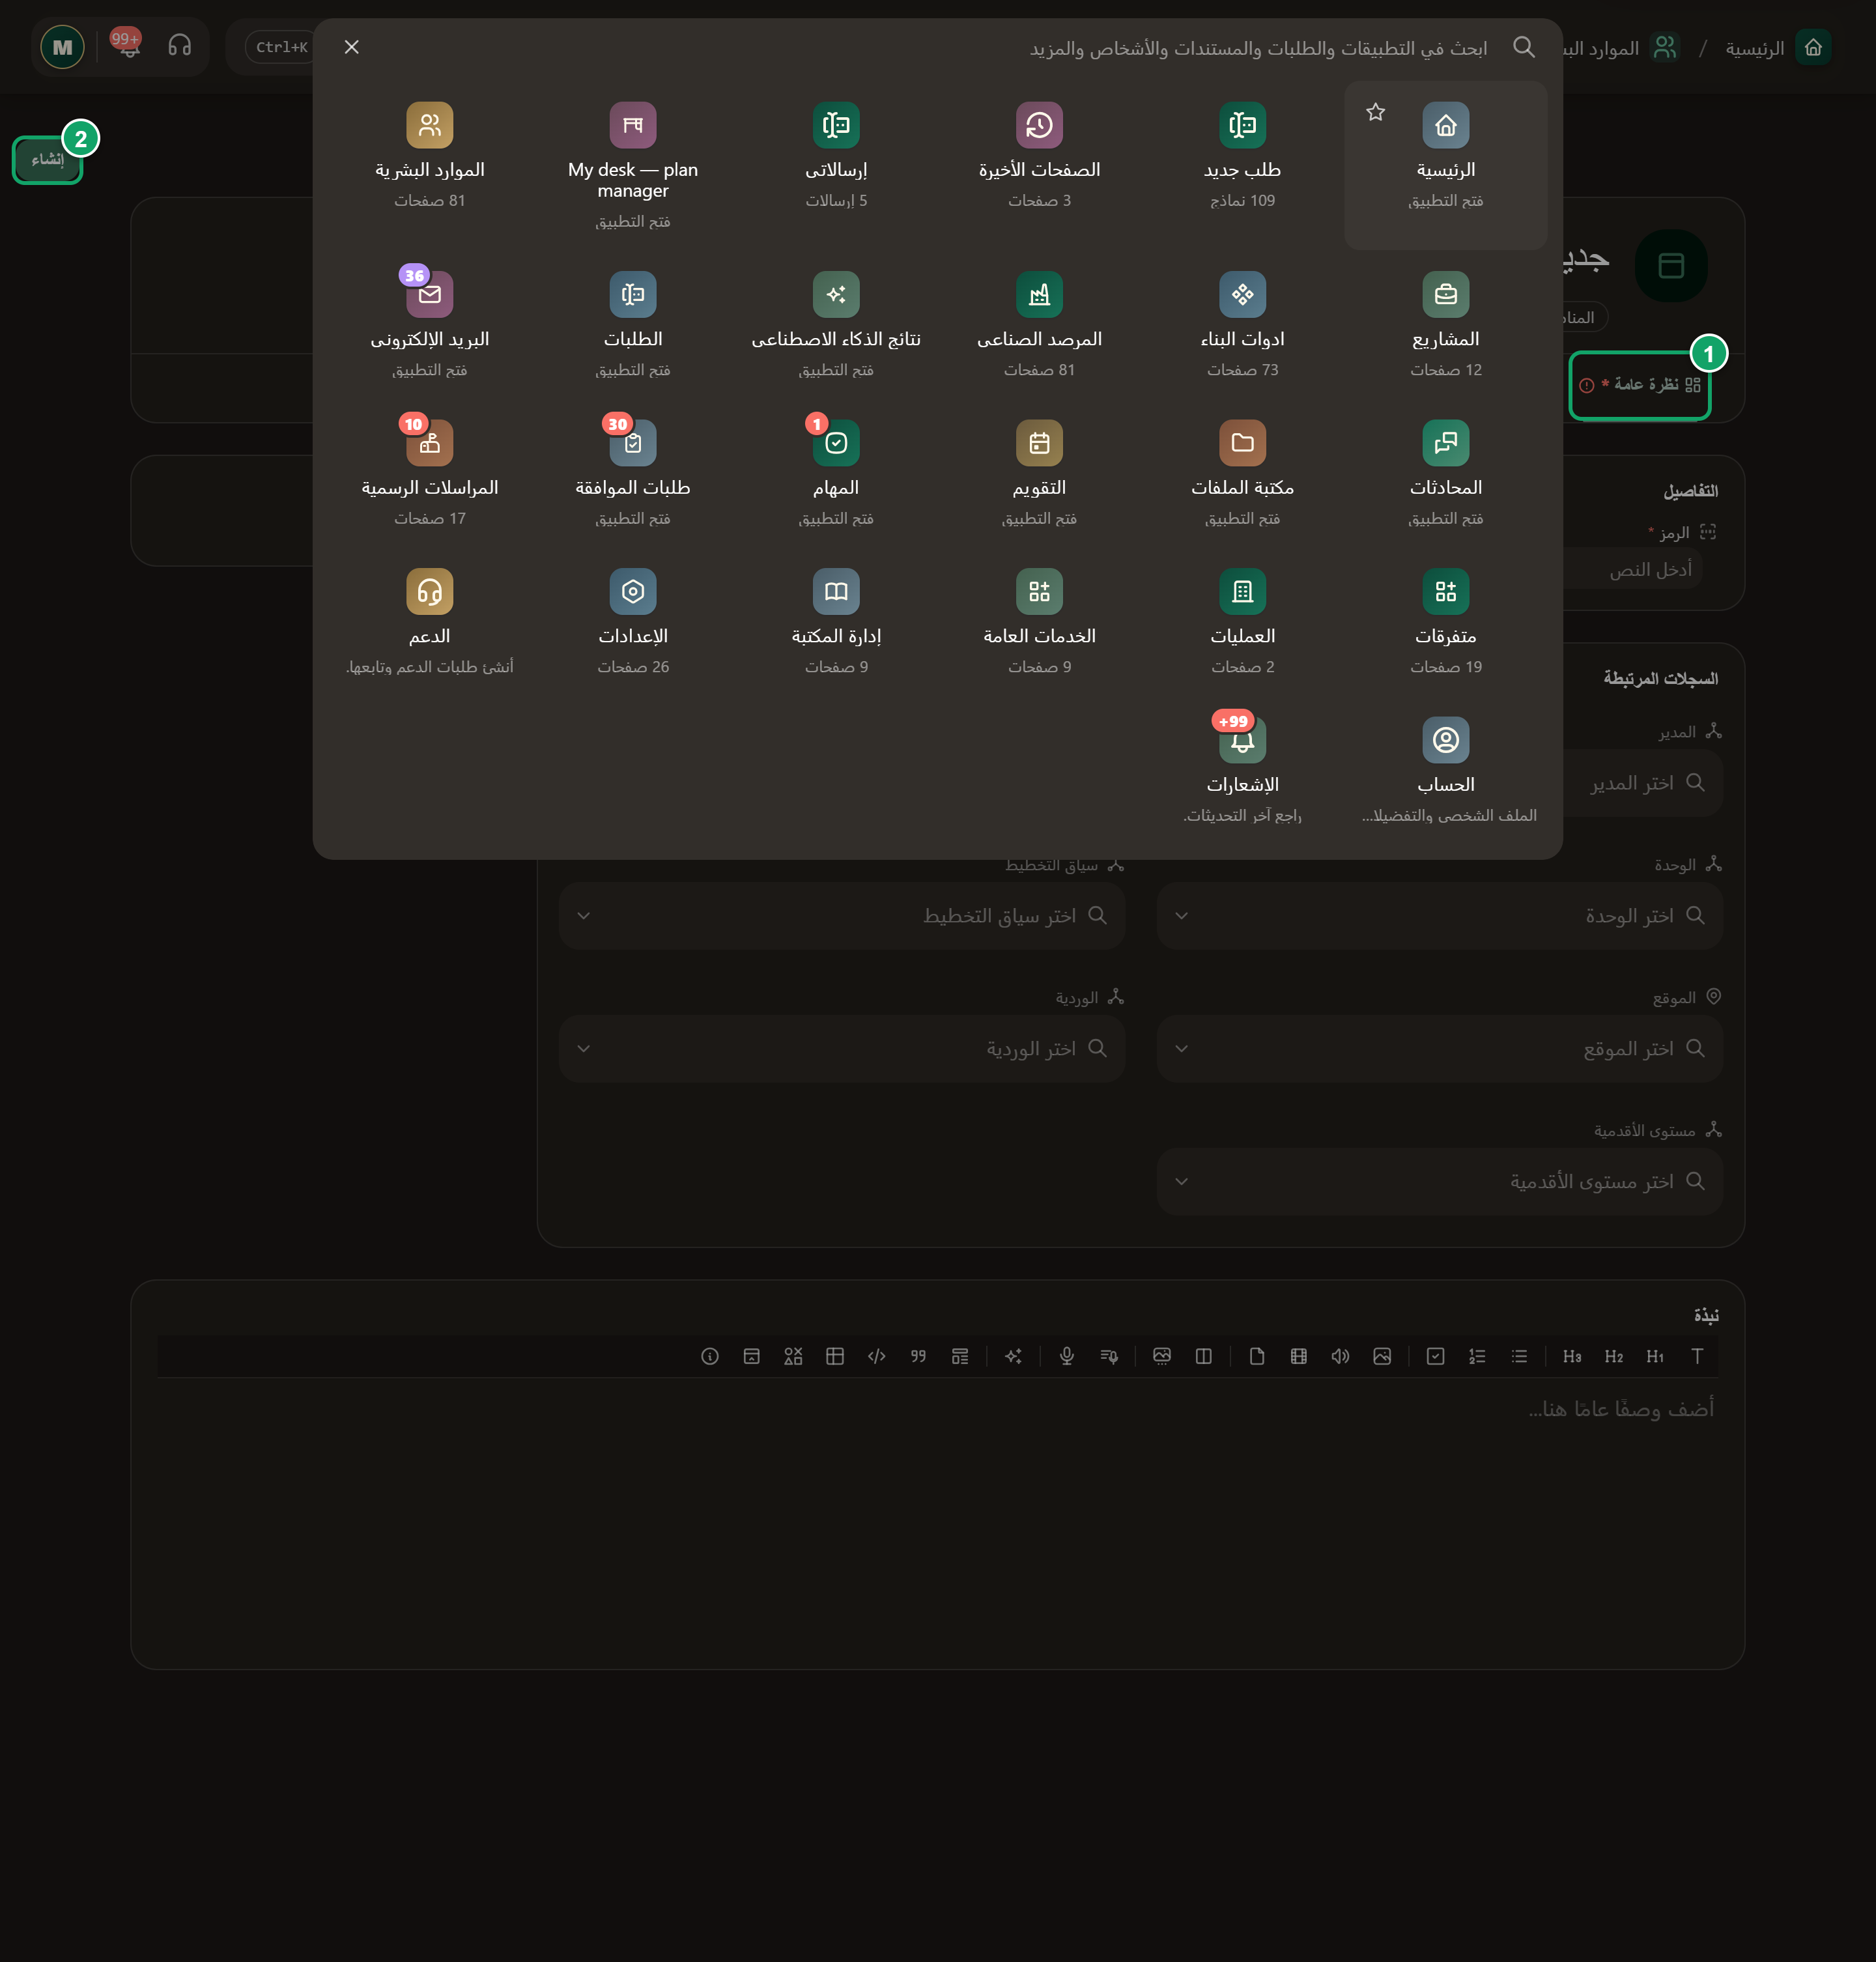
\includegraphics[width=0.95\linewidth]{figures/screens/ch02-position-fields-ar.png}
\caption{المناصب: نموذج من بيئة الاختبار؛ لم يُحفظ}
\label{fig:hr-feature-positions-screen}
\end{figure}

\begin{table}[H]
\centering
\caption{ما الذي تسجله في المنصب؟}
\label{tab:hr-feature-positions-data}
\rcZebra
\begin{tabularx}{\linewidth}{R{3.6cm} Y}
\rcHeaderRow
\thh{الحقل} & \thh{ما الذي تضيفه؟}\\
الرمز والاسم & \req{}؛ مثل \en{HZN-P-01} مدير الموارد البشرية.\\
المدير & المنصب الذي يتبعه هذا المنصب؛ ومنه تُبنى شجرة الهيكل الوظيفي.\\
الوصف الوظيفي & المهام والمسؤوليات؛ تختاره من قائمة الأوصاف أو تكتب وصفاً جديداً.\\
الوحدة والموقع & القسم ومكان العمل \opt{}.\\
الوردية والمستوى الوظيفي & دوام الوظيفة ودرجتها في سلم الراتب \opt{}.\\
سياق التخطيط & خطة أو مشروع أو برنامج ترتبط به الوظيفة \opt{}.\\
\end{tabularx}
\end{table}

\subsection{ما الذي يمكنك فعله؟}

\begin{itemize}
  \item عرض «شجرة»: ابحث بالمنصب أو الرمز أو الشخص، وسّع الفروع أو اطوِها، واختر «إظهار هذا الفرع فقط».
  \item كل بطاقة في الشجرة تبيّن شاغل المنصب أو «شاغر»، وعدد المناصب التابعة.
  \item يعرض النظام شاغلي المنصب الحاليين \gen{}.
\end{itemize}

\begin{figure}[H]
\centering
\begin{tikzpicture}[node distance=0.5cm,stepBox/.append style={minimum width=6.5cm,text width=6.1cm,minimum height=0.8cm}]
  \node[stepBox] (a) {\RL{تعريف الوظيفة}};
  \node[stepBox,below=of a] (b) {\RL{اختيار القسم والموقع}};
  \node[stepBox,below=of b] (c) {\RL{تعيين الموظف}};
  \draw[flowsTo] (a) -- (b);
  \draw[flowsTo] (b) -- (c);
\end{tikzpicture}
\rclegend
\caption{خطوات الاستخدام؛ الأسهم لا تعني معالجة تلقائية}
\label{fig:hr-feature-positions-flow}
\end{figure}

\subsection{جرّب وراجع}

\begin{enumerate}
  \item جهّز القسم والموقع إن أردت ربطهما. افتح «المناصب» وتأكد أن الوظيفة غير موجودة.
  \item أضف «مدير الموارد البشرية» برمز \en{HZN-P-01}، واختر قسم الموارد البشرية والمقر الرئيسي بدمشق، ثم احفظ.
\end{enumerate}

\textbf{تحقق:} أعد فتح المنصب وتحقق من روابطه، ثم افتح الشجرة. إنشاء المنصب لا يعيّن سارة فيه.

\begin{figure}[H]
\centering
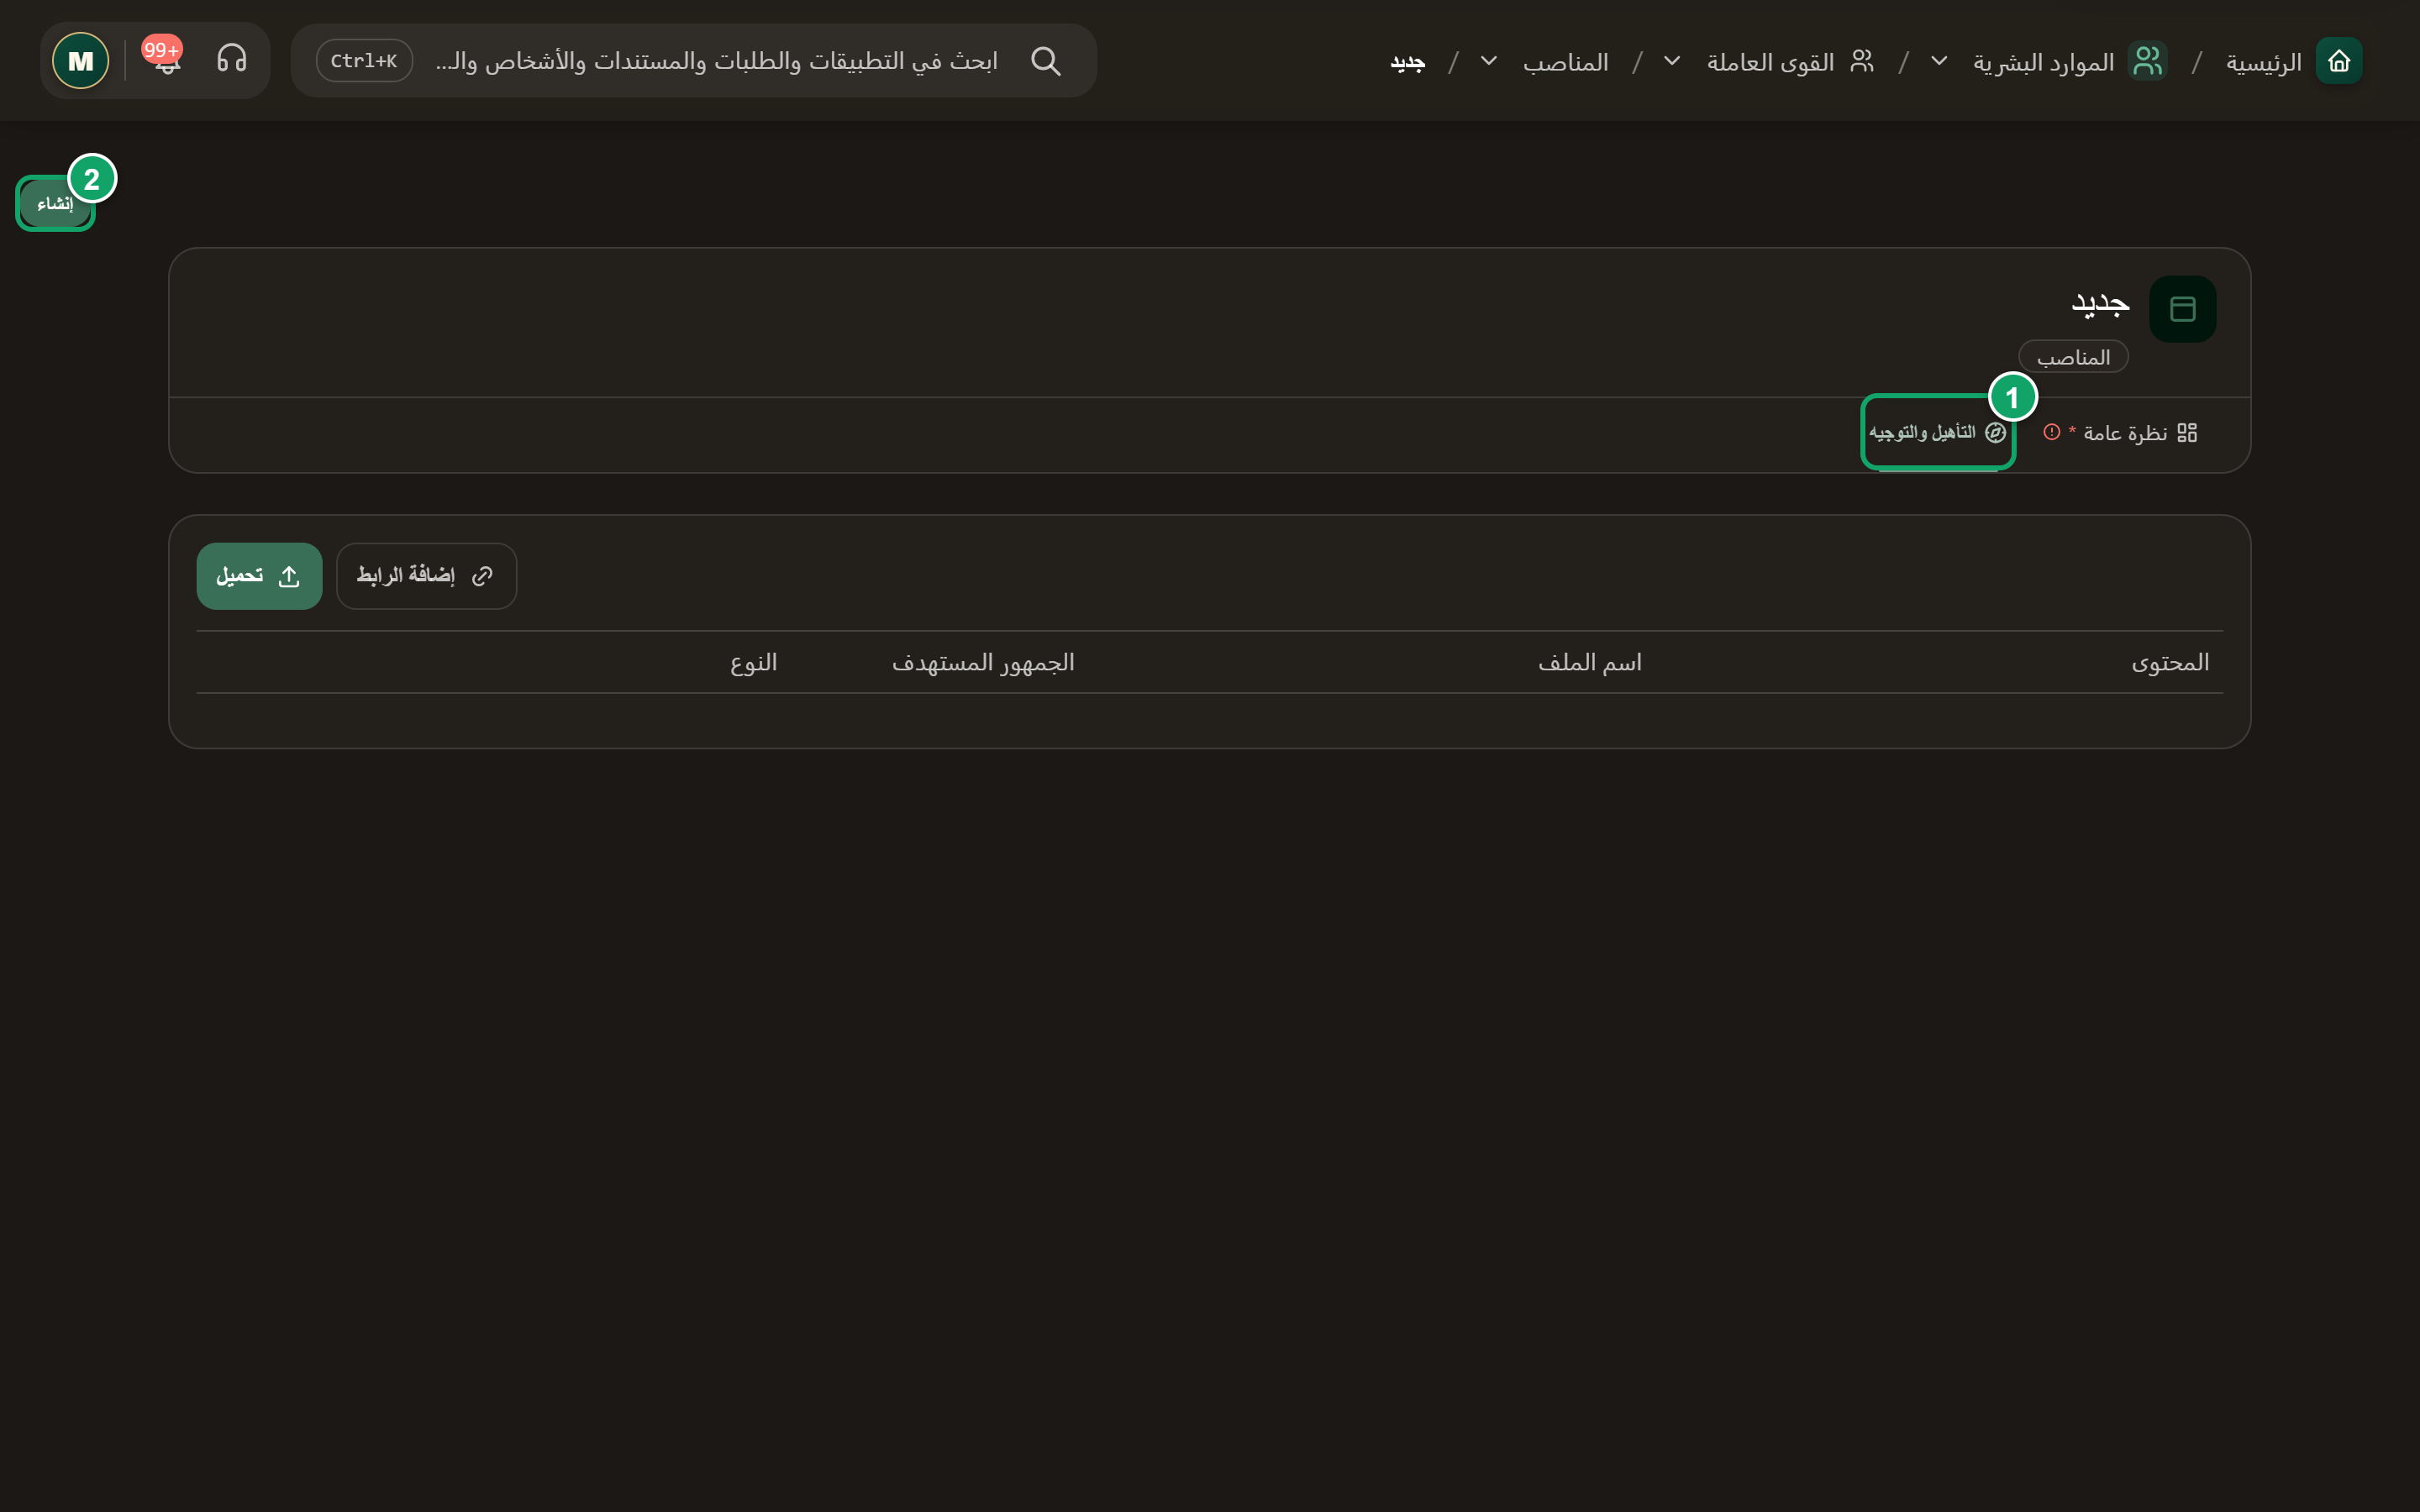
\includegraphics[width=0.95\linewidth]{figures/screens/ch02-position-fields-tab2-ar.png}
\caption{تبويب «التأهيل والتوجيه» كاملاً؛ نموذج غير محفوظ}
\label{fig:hr-positions-fulltab1}
\end{figure}

\clearpage
\section{التعيينات}
\label{sec:hr-feature-assignments}

التعيين يسجل من يشغل المنصب، ومنذ متى، وبأي عقد وراتب ووردية.

\textbf{متى تفيد؟} عند انضمام سارة أو انتقالها إلى وظيفة أخرى. يحفظ التعيين وظائفها وتواريخها منفصلة عن ملفها الشخصي. \textbf{المسار:} «الموارد البشرية» / «القوى العاملة» / «التعيينات».

\begin{figure}[H]
\centering
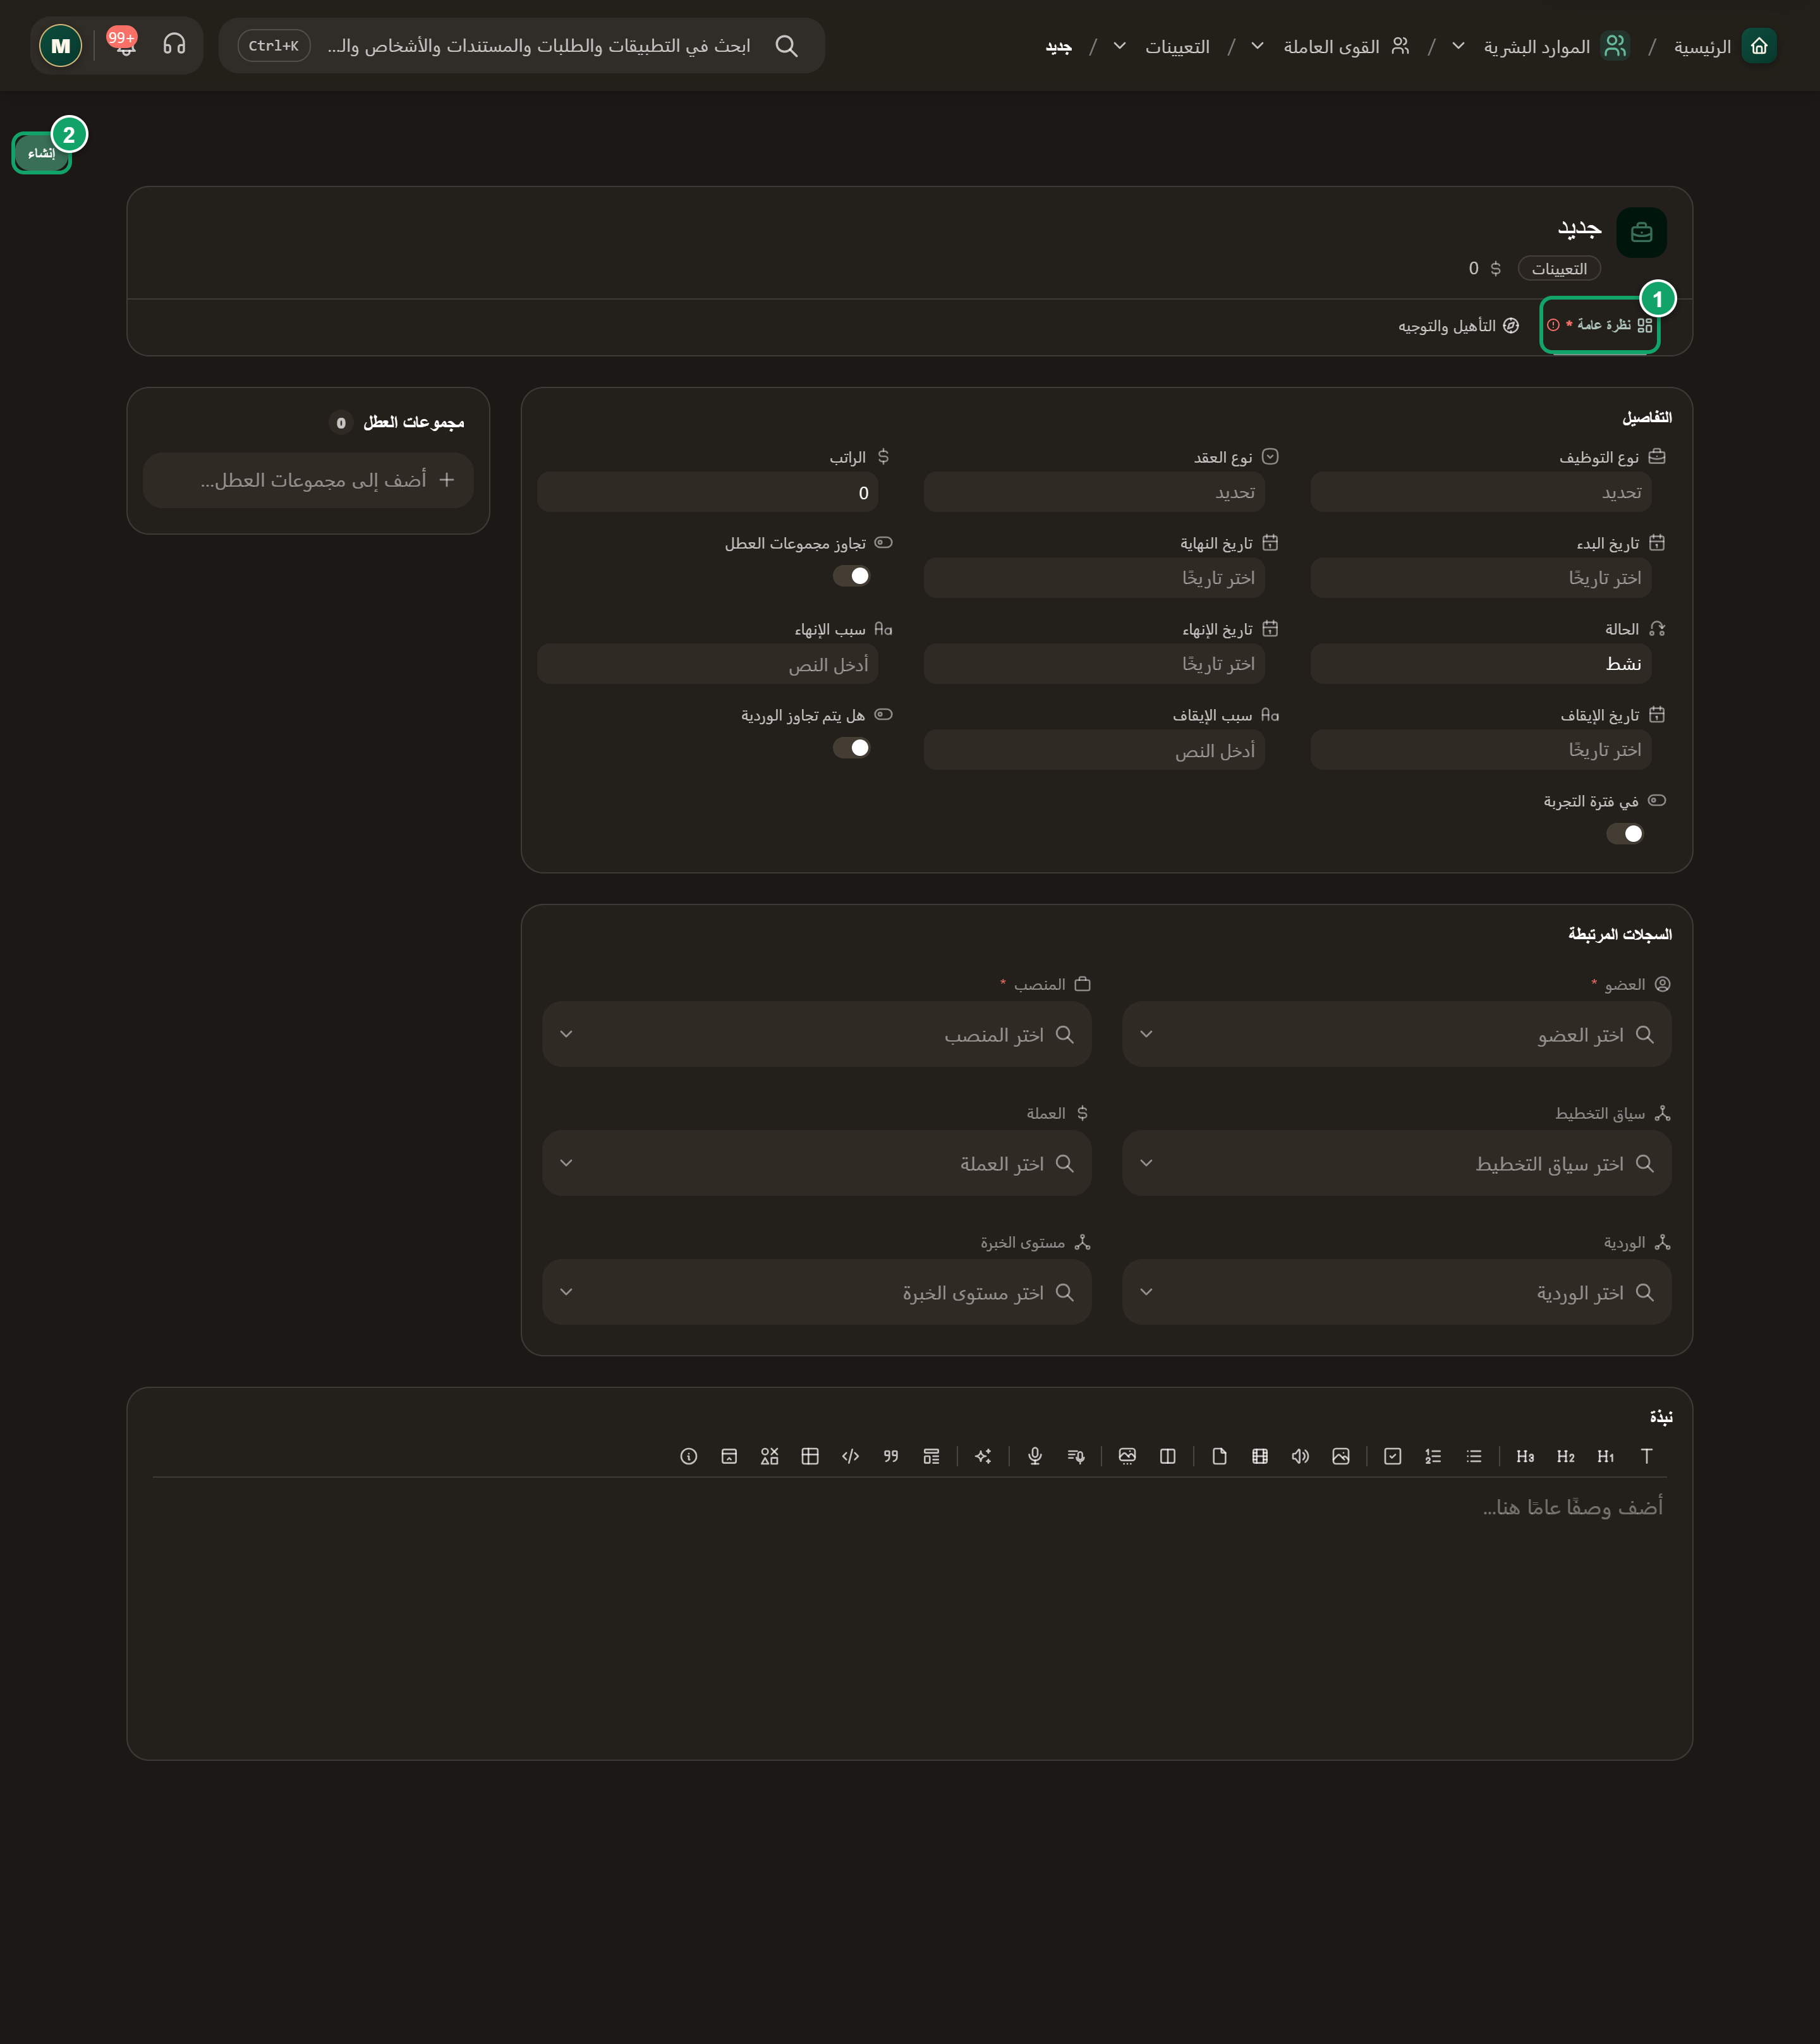
\includegraphics[width=0.95\linewidth]{figures/screens/ch02-assignment-fields-ar.png}
\caption{التعيينات: نموذج من بيئة الاختبار؛ لم يُحفظ}
\label{fig:hr-feature-assignments-screen}
\end{figure}

\begin{table}[H]
\centering
\caption{ما الذي تسجله في التعيين؟}
\label{tab:hr-feature-assignments-data}
\rcZebra
\begin{tabularx}{\linewidth}{R{3.6cm} Y}
\rcHeaderRow
\thh{الجزء} & \thh{ما الذي تضيفه؟}\\
الشخص والوظيفة & العضو \req{} والمنصب \req{}.\\
العقد & نوع التوظيف: موظف، مقاول، متطوع، متدرب، قائم بأعمال، عند الطلب. نوع العقد: دائم، محدد المدة، مؤقت.\\
الفترة & تاريخ البدء وتاريخ النهاية، وفترة التجربة وتاريخ انتهائها.\\
الراتب & الراتب والعملة ومستوى الخبرة.\\
الوقت & الوردية وتجاوزها، ومجموعات العطل وتجاوزها.\\
الحالة & نشط، متوقف، منتهي، مكتمل؛ مع تاريخ الإيقاف أو الإنهاء وسببه.\\
\end{tabularx}
\end{table}

\subsection{ما الذي يمكنك فعله؟}

\begin{itemize}
  \item عرض القائمة جدولاً، أو لوحة كانبان حسب الحالة، أو تقويماً أو خطاً زمنياً حسب تواريخ البدء والنهاية.
  \item ابدأ التعيين من ملف العضو باختيار «إضافة تعيين».
  \item حفظ التعيين يحدّث مناصب العضو النشطة وشاغلي المنصب \gen{}.
\end{itemize}

\begin{figure}[H]
\centering
\begin{tikzpicture}[node distance=0.5cm,stepBox/.append style={minimum width=6.5cm,text width=6.1cm,minimum height=0.8cm}]
  \node[stepBox] (a) {\RL{تجهيز العضو والمنصب}};
  \node[stepBox,below=of a] (b) {\RL{حفظ التعيين}};
  \node[stepBox,below=of b] (c) {\RL{مراجعة الفترة}\\\RL{والوردية}};
  \draw[flowsTo] (a) -- (b);
  \draw[flowsTo] (b) -- (c);
\end{tikzpicture}
\rclegend
\caption{خطوات الاستخدام؛ الأسهم لا تعني معالجة تلقائية}
\label{fig:hr-feature-assignments-flow}
\end{figure}

\subsection{جرّب وراجع}

\begin{enumerate}
  \item جهّز سجل سارة ومنصب مدير الموارد البشرية، أو ابحث عنهما.
  \item أضف تعييناً: سارة، مدير الموارد البشرية، «موظف»، «دائم»، وتاريخ البدء الفعلي. اترك الحالة «نشط» واحفظ.
\end{enumerate}

\textbf{تحقق:} أعد الفتح وتحقق من الشخص والمنصب والفترة والحالة. عند تغيّر الوظيفة، أنهِ التعيين القديم وأضف جديداً؛ لا تنشئ عضواً آخر.

\begin{figure}[H]
\centering
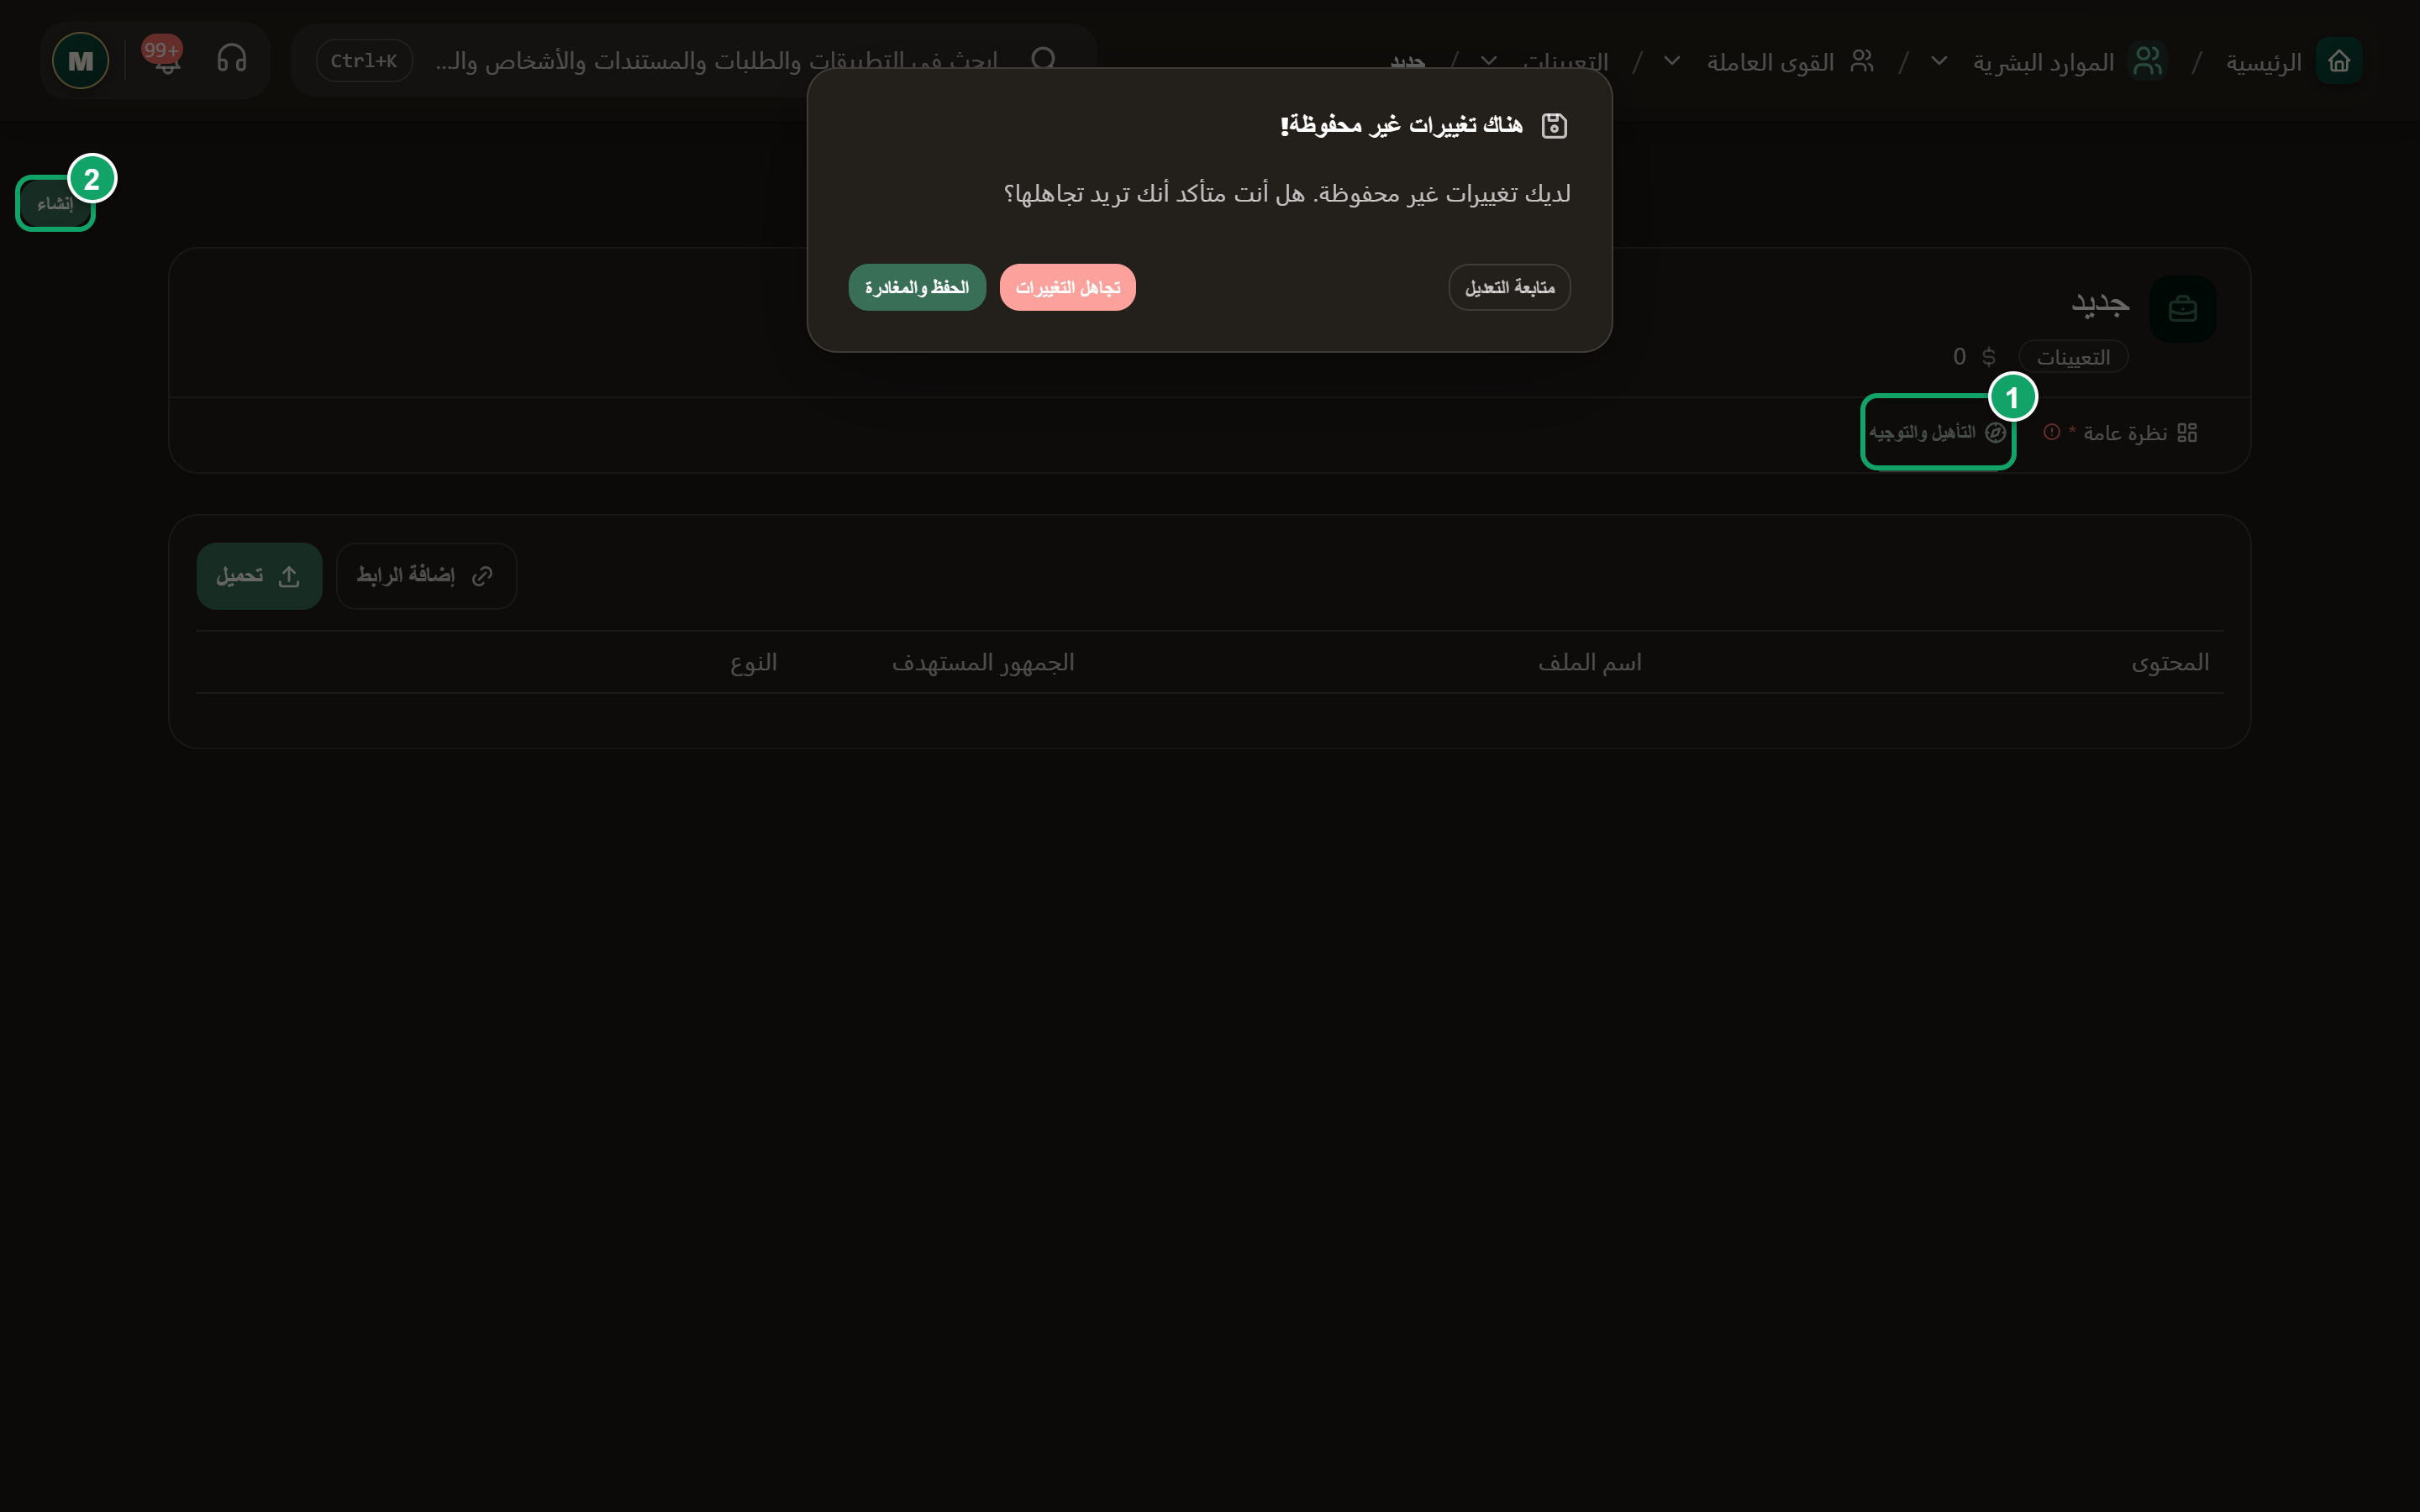
\includegraphics[width=0.95\linewidth]{figures/screens/ch02-assignment-fields-tab2-ar.png}
\caption{تبويب «التأهيل والتوجيه» كاملاً؛ نموذج غير محفوظ}
\label{fig:hr-assignments-fulltab1}
\end{figure}

\clearpage
\section{الوحدات التنظيمية}
\label{sec:hr-feature-nodes}

الوحدة التنظيمية قسم أو إدارة. حقل «يتبع ل» يضعها في شجرة الهيكل. وهي تحدد الجهة التي تتبعها الوظيفة، لا مكان العمل.

\textbf{متى تفيد؟} توضح الهيكل مع توسع الفريق. في شركة الأفق، تتبع الموارد البشرية الإدارة العامة. \textbf{المسار:} «الموارد البشرية» / «الأساسية» / «الوحدات التنظيمية».

\begin{figure}[H]
\centering
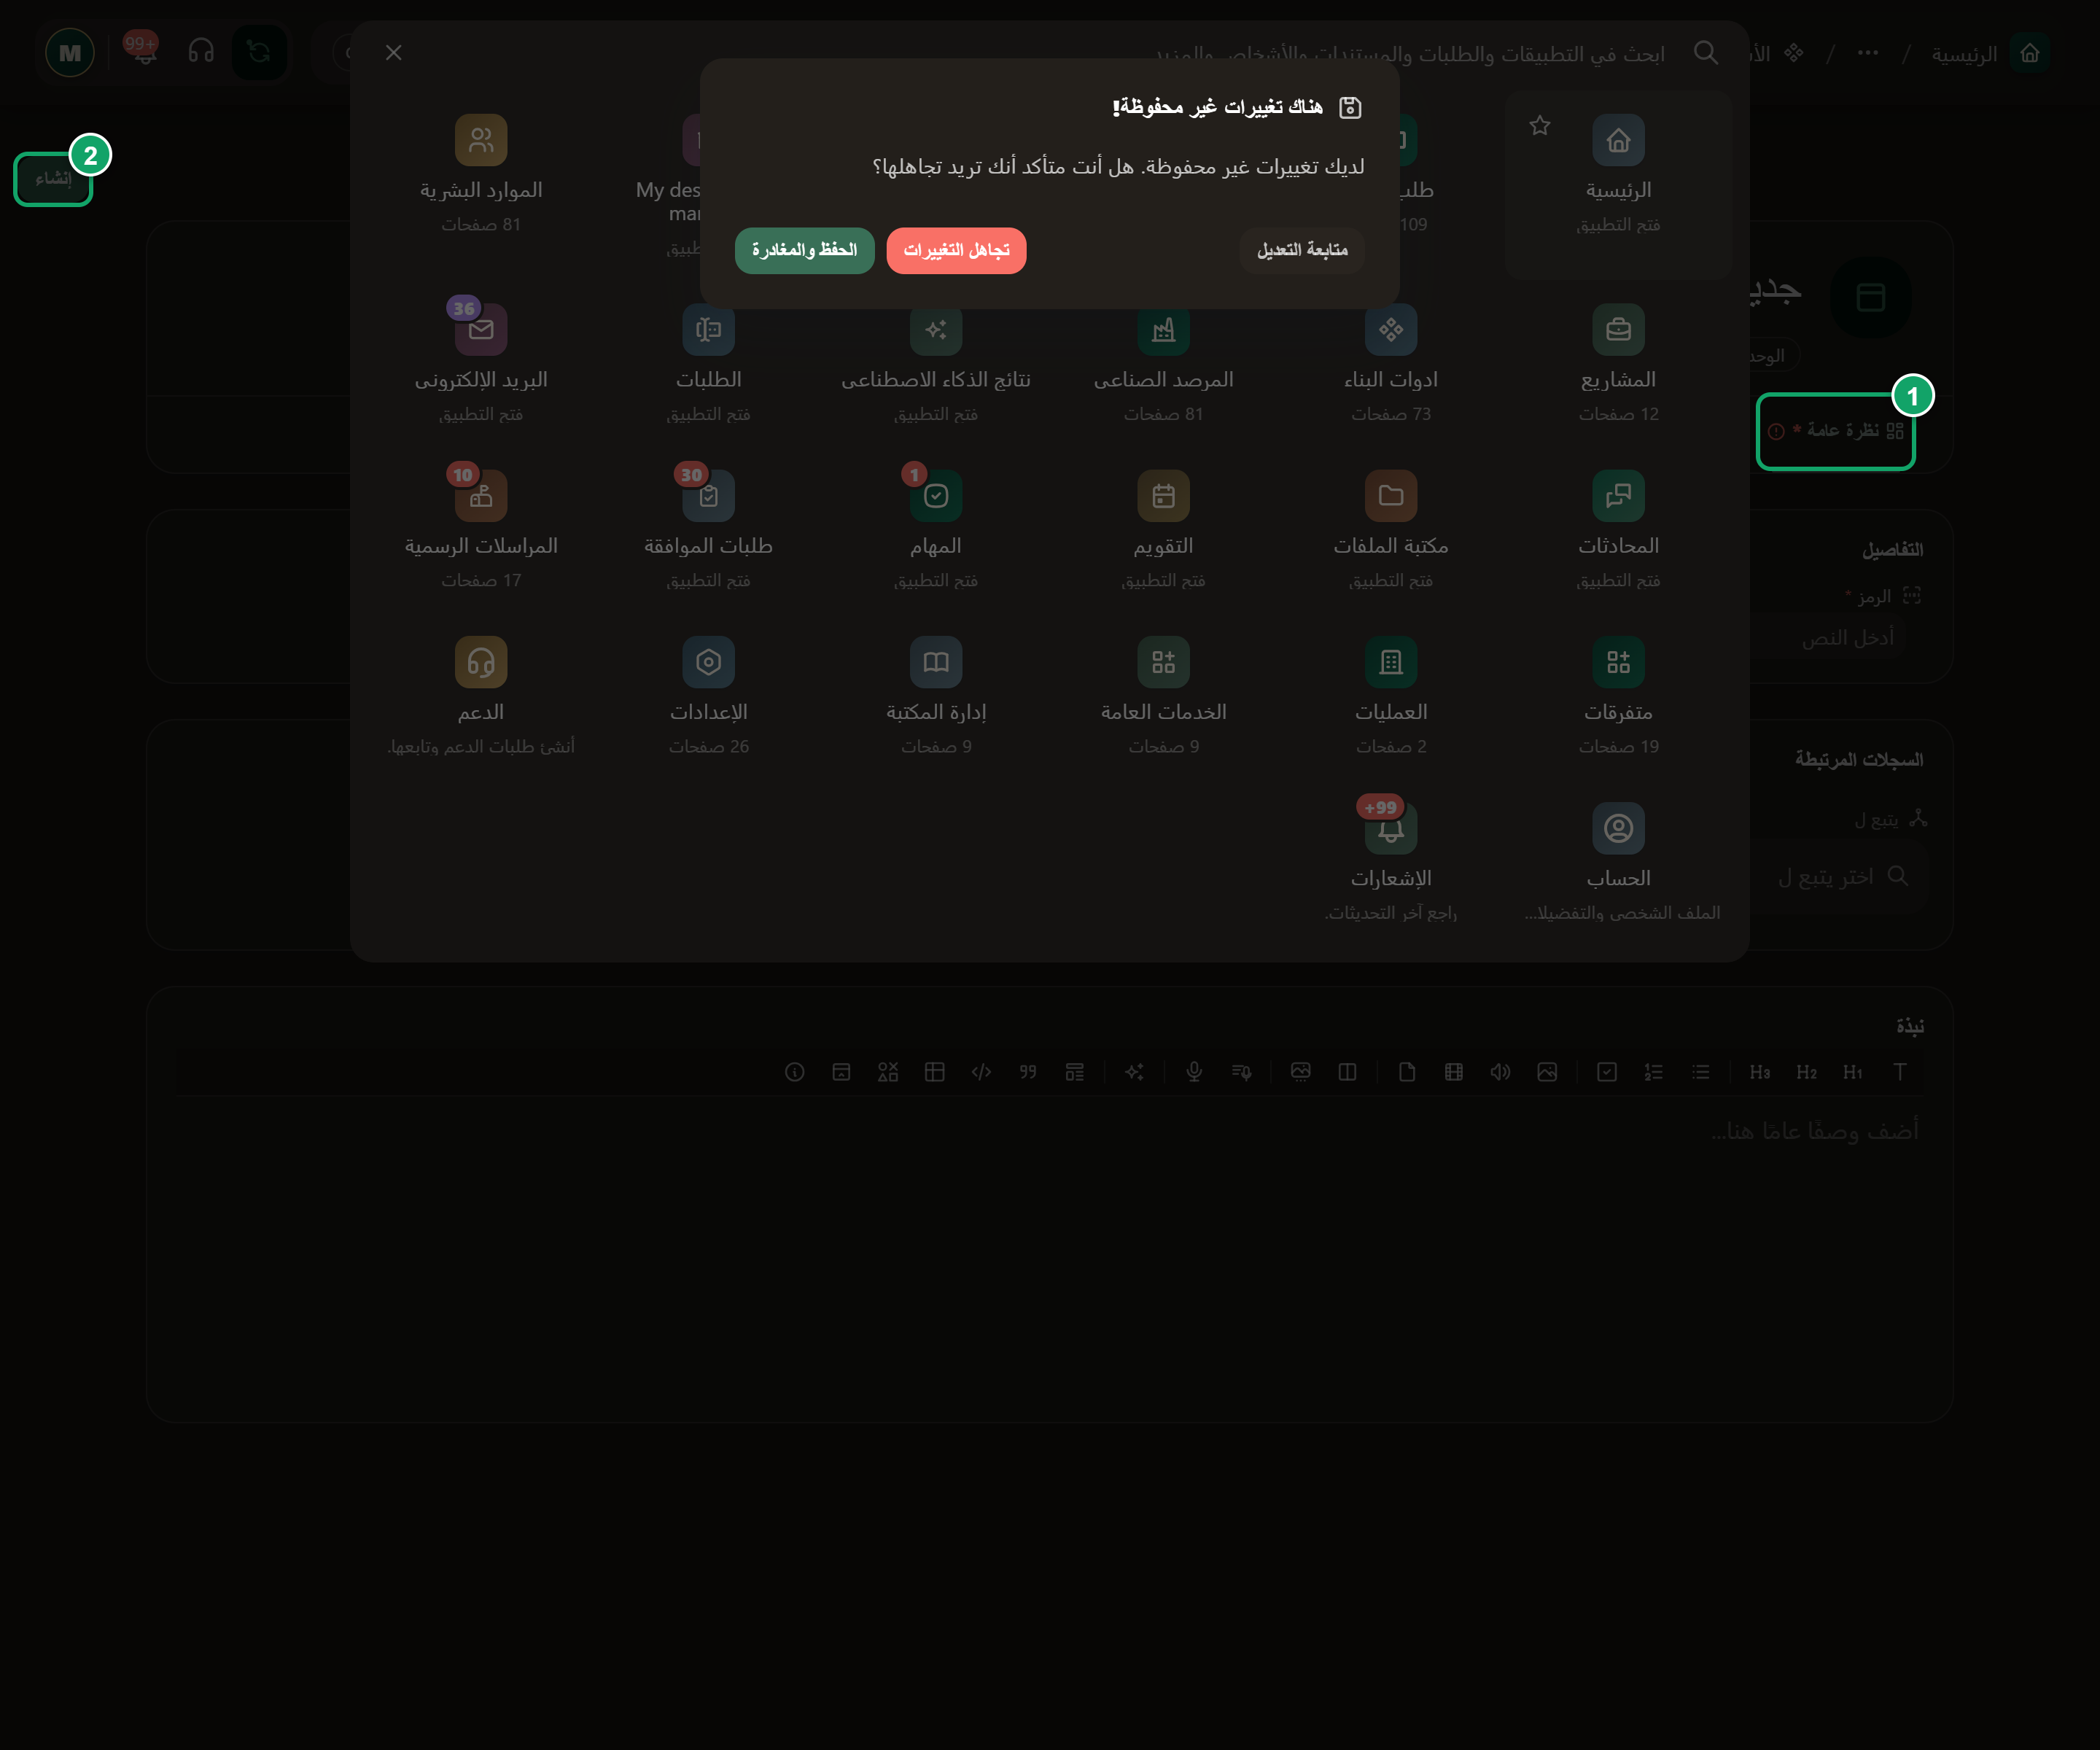
\includegraphics[width=0.95\linewidth]{figures/screens/ch02-node-fields-ar.png}
\caption{الوحدات التنظيمية: نموذج من بيئة الاختبار؛ لم يُحفظ}
\label{fig:hr-feature-nodes-screen}
\end{figure}

\begin{table}[H]
\centering
\caption{ما الذي تسجله في الوحدة؟}
\label{tab:hr-feature-nodes-data}
\rcZebra
\begin{tabularx}{\linewidth}{R{3.6cm} Y}
\rcHeaderRow
\thh{الحقل} & \thh{ما الذي تضيفه؟}\\
الرمز والاسم والنوع & \req{}؛ الأنواع يعرّفها مسؤول المؤسسة، مثل إدارة أو قسم.\\
يتبع ل & الوحدة الأم، مثل \en{HZN-GM} للموارد البشرية.\\
الوردية & تُورث من الوحدة الأم، أو تُستبدل بها وردية خاصة.\\
نظرة عامة والتأهيل والتوجيه & وصف الوحدة، ومواد تعريف الموظف الجديد بها.\\
\end{tabularx}
\end{table}

\subsection{ما الذي يمكنك فعله؟}

\begin{itemize}
  \item عرض «شجرة» مع البحث؛ كل بطاقة تبين المناصب والموظفين والشواغر.
  \item «مع الفروع» أو «بدون الفروع»: لتحديد إن كانت الأعداد تشمل الوحدات التابعة.
  \item «تجاوز» لاستبدال الوردية الموروثة، و«إعادة تعيين» لاستعادتها.
\end{itemize}

\begin{figure}[H]
\centering
\begin{tikzpicture}[node distance=0.5cm,stepBox/.append style={minimum width=6.5cm,text width=6.1cm,minimum height=0.8cm}]
  \node[stepBox] (a) {\RL{إنشاء الإدارة العامة}};
  \node[stepBox,below=of a] (b) {\RL{إضافة الموارد البشرية}\\\RL{تحتها}};
  \node[stepBox,below=of b] (c) {\RL{ربط منصب مدير الموارد}\\\RL{البشرية}};
  \draw[flowsTo] (a) -- (b);
  \draw[flowsTo] (b) -- (c);
\end{tikzpicture}
\rclegend
\caption{خطوات الاستخدام؛ الأسهم لا تعني معالجة تلقائية}
\label{fig:hr-feature-nodes-flow}
\end{figure}

\subsection{جرّب وراجع}

\begin{enumerate}
  \item افتح «الوحدات التنظيمية». إن لم تكن الإدارة العامة موجودة، أضفها برمز \en{HZN-GM} واختر نوعها ثم احفظ.
  \item أضف «الموارد البشرية» برمز \en{HZN-HR}، واختر النوع، والإدارة العامة في «يتبع ل»، ثم احفظ.
\end{enumerate}

\textbf{تحقق:} افتح الشجرة وتأكد أن الموارد البشرية تحت الإدارة العامة. ربط المنصب بالوحدة اختياري ولا يغني عن تعيين سارة.

\begin{figure}[H]
\centering
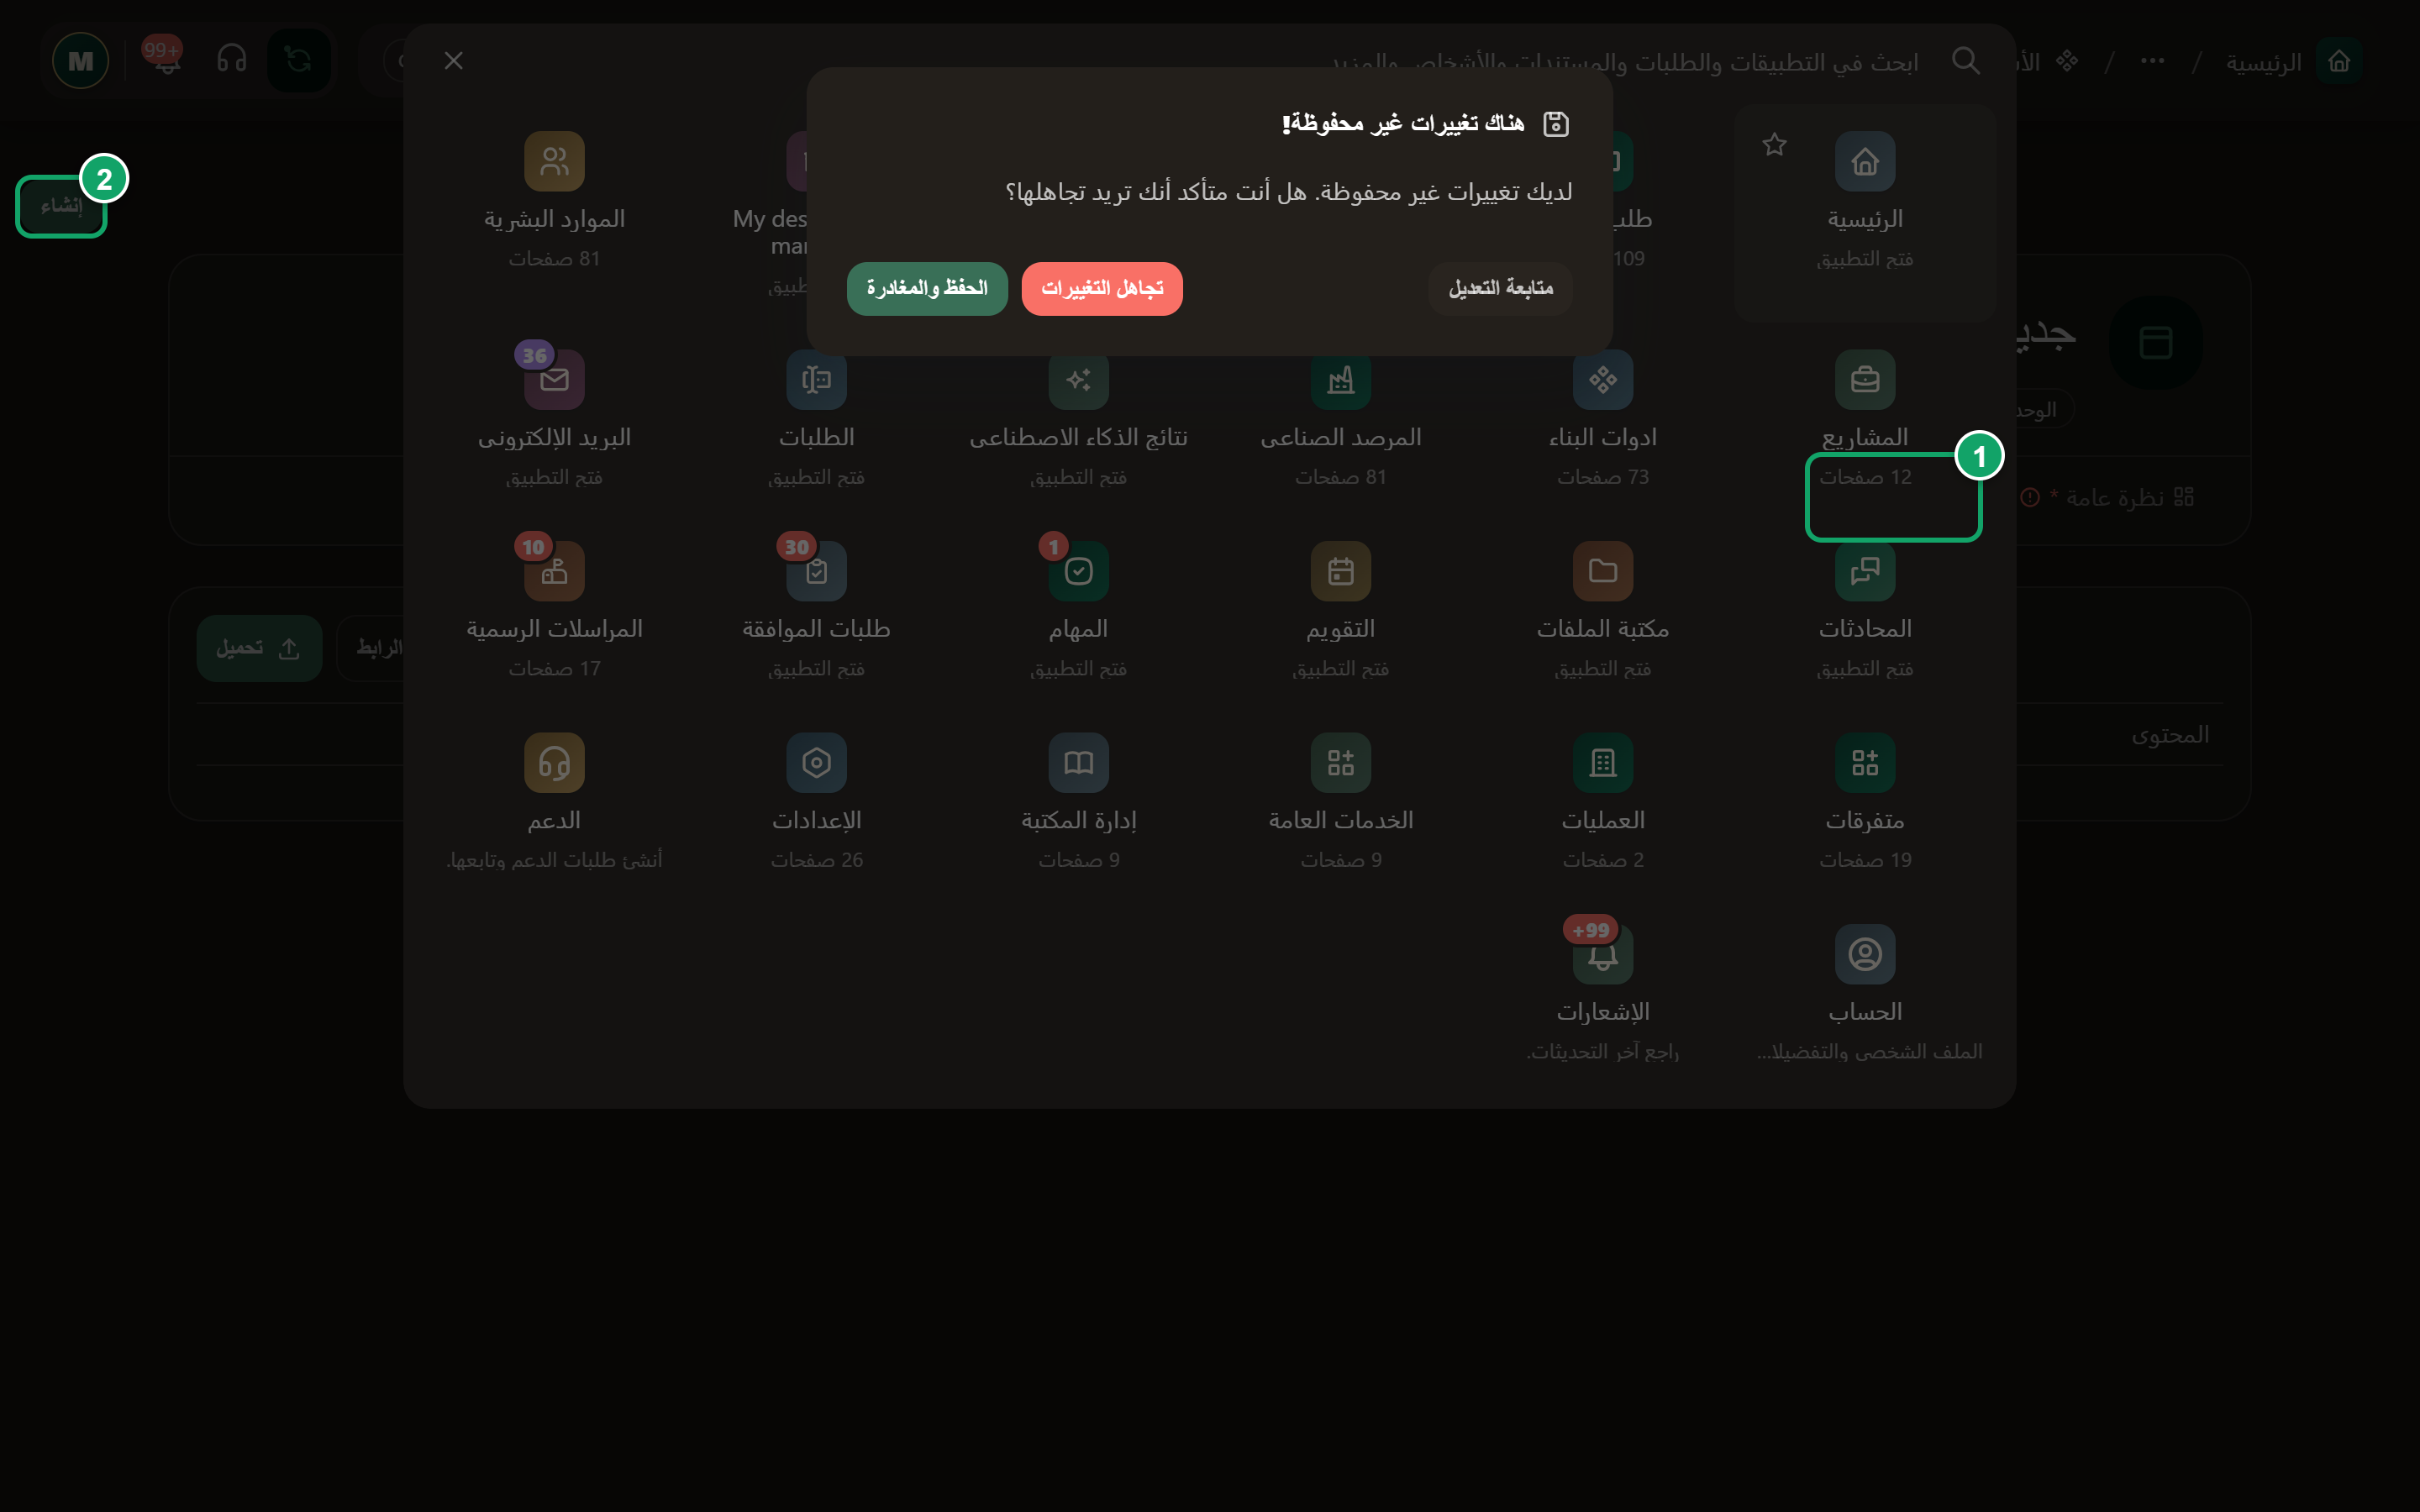
\includegraphics[width=0.95\linewidth]{figures/screens/ch02-node-fields-tab2-ar.png}
\caption{تبويب «التأهيل والتوجيه» كاملاً؛ نموذج غير محفوظ}
\label{fig:hr-nodes-fulltab1}
\end{figure}

\clearpage
\section{النقاط الجغرافية}
\label{sec:hr-feature-locations}

النقطة الجغرافية مكان عمل، مثل مكتب أو فرع، بعنوانه ونقطته على الخريطة. ويمكن أن يتبع موقعاً آخر.

\textbf{متى تفيد؟} تفصل المكان عن القسم: قسمان في مقر دمشق، أو قسم واحد في عدة مواقع. \textbf{المسار:} «الموارد البشرية» / «الأساسية» / «النقاط الجغرافية».

\begin{figure}[H]
\centering
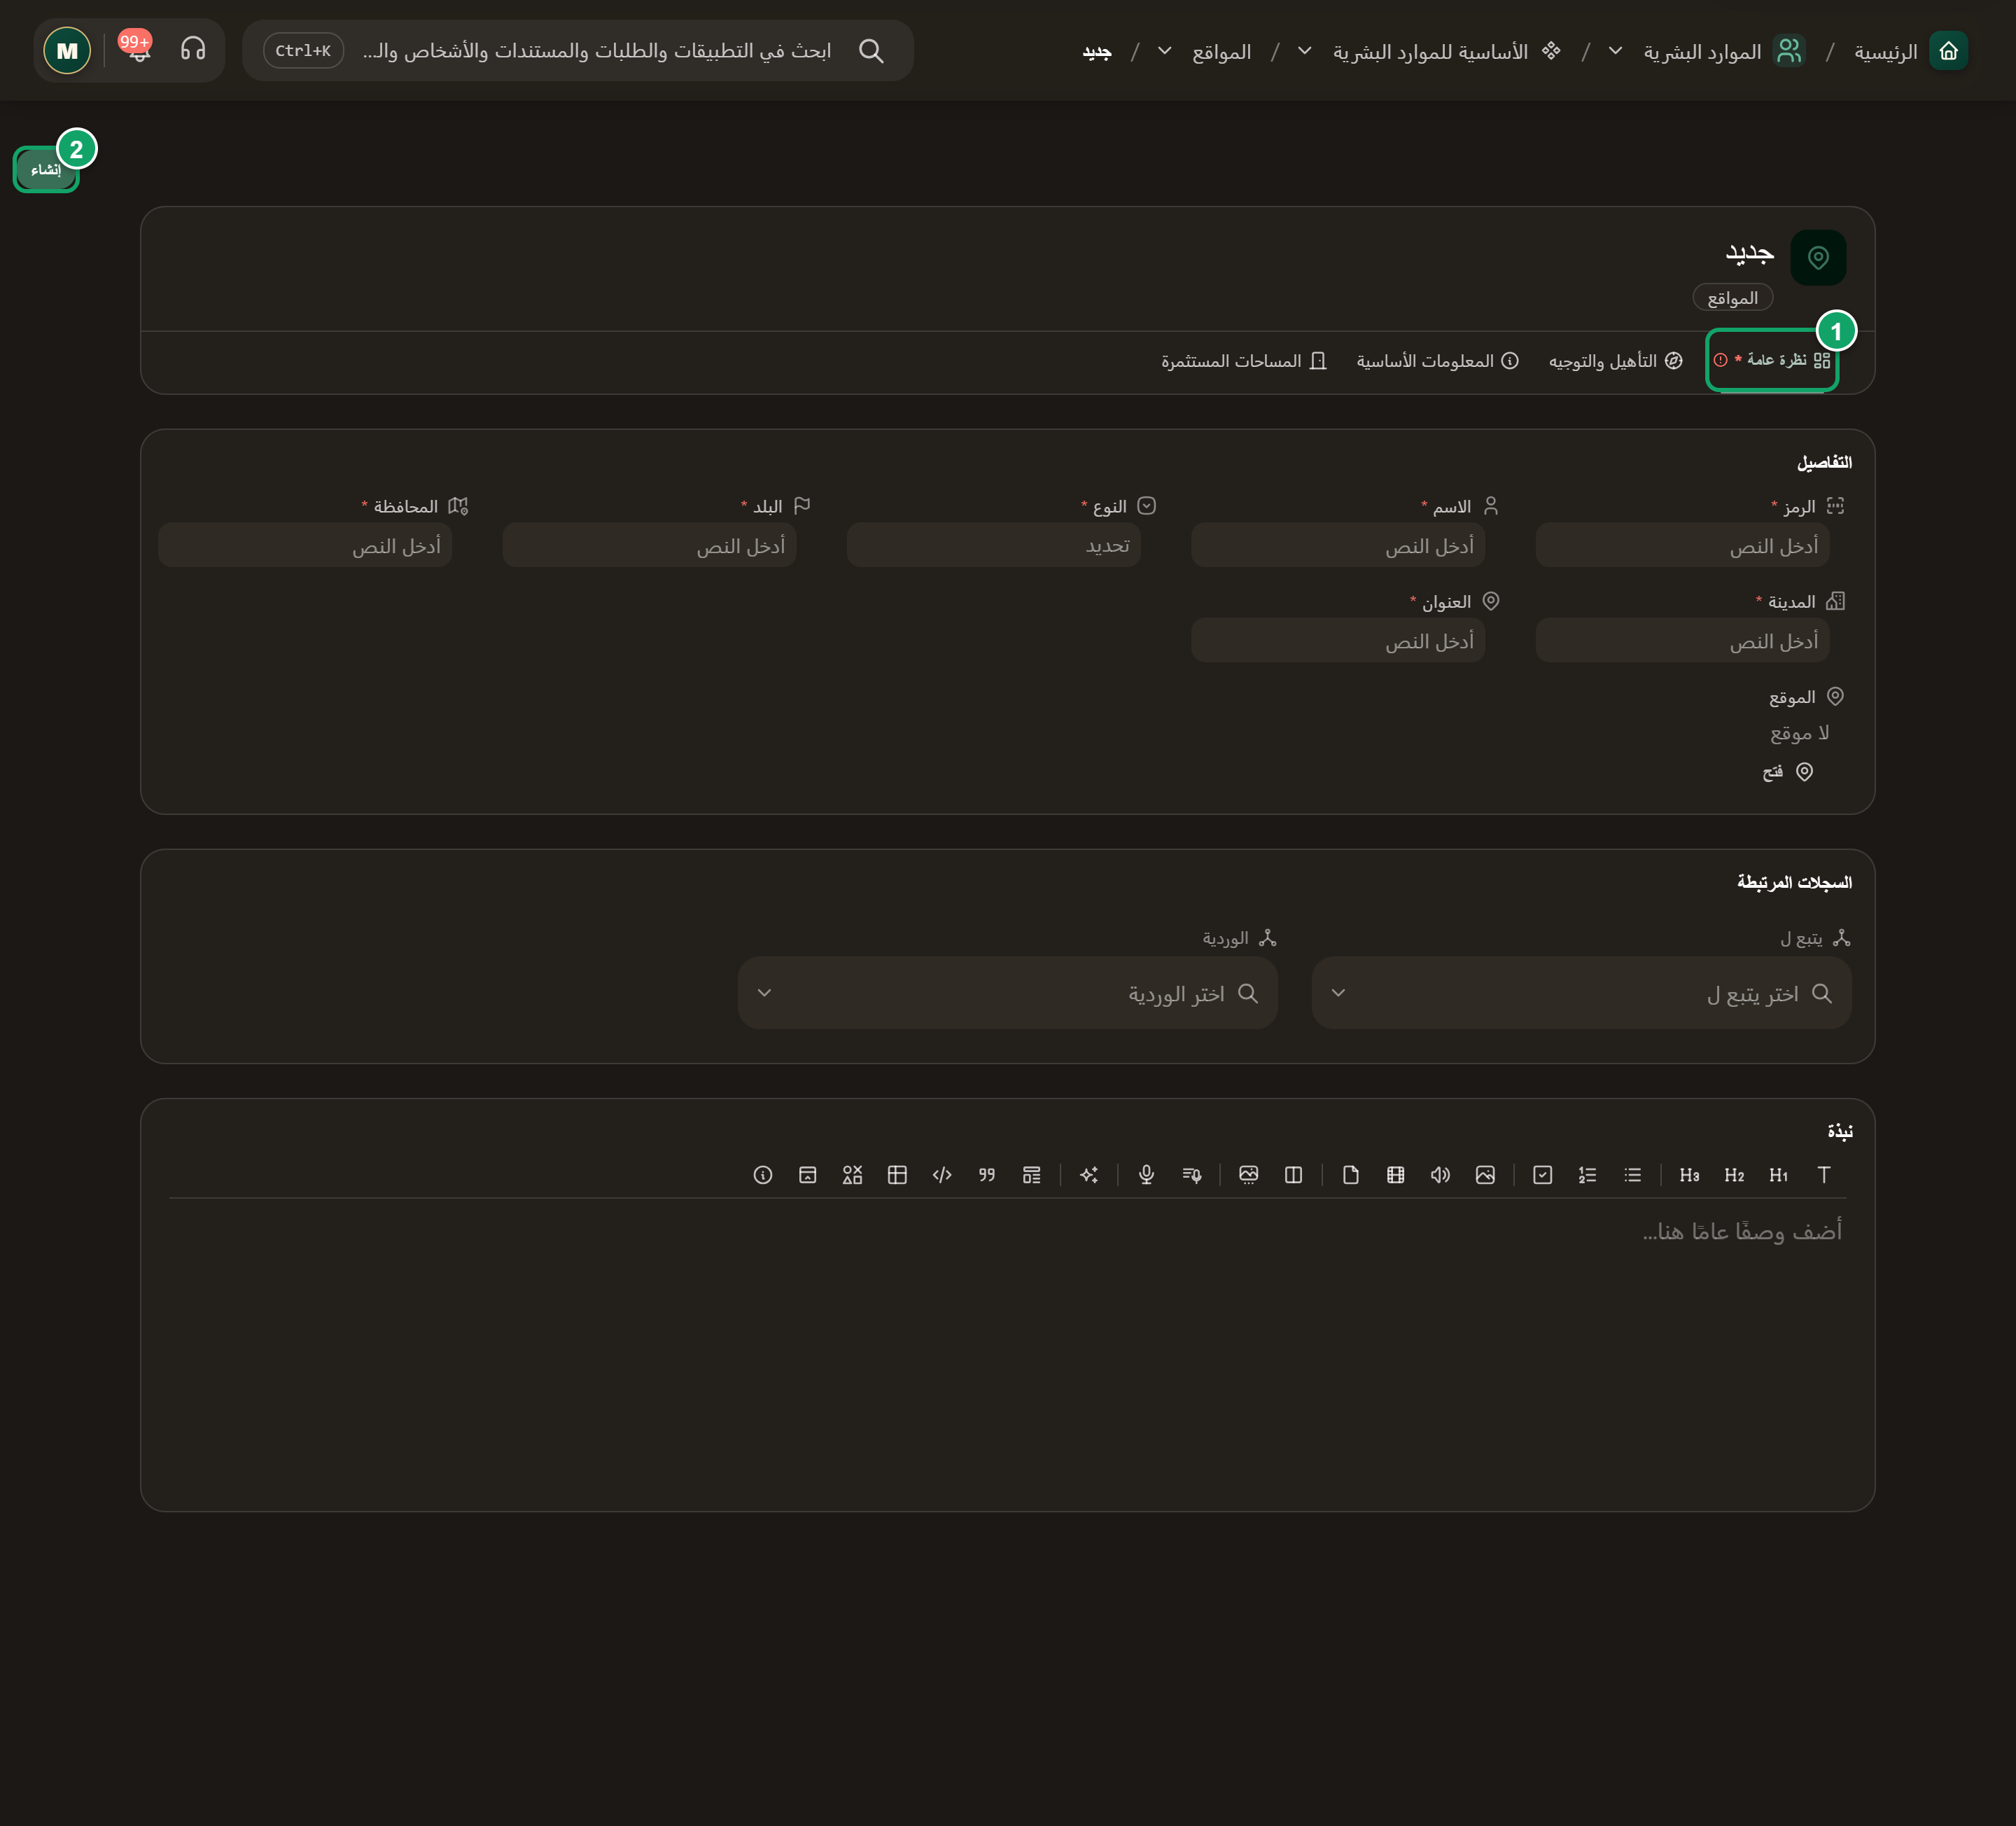
\includegraphics[width=0.95\linewidth]{figures/screens/ch02-location-fields-ar.png}
\caption{النقاط الجغرافية: نموذج من بيئة الاختبار؛ لم يُحفظ}
\label{fig:hr-feature-locations-screen}
\end{figure}

\begin{table}[H]
\centering
\caption{ما الذي تسجله في الموقع؟}
\label{tab:hr-feature-locations-data}
\rcZebra
\begin{tabularx}{\linewidth}{R{3.6cm} Y}
\rcHeaderRow
\thh{التبويب أو الحقل} & \thh{ما الذي تضيفه؟}\\
الأساسية & الرمز والاسم والنوع \req{}؛ الموقع الأم والوردية \opt{}.\\
العنوان & البلد والمحافظة والمدينة والعنوان \req{}، ونقطة على الخريطة.\\
المعلومات الأساسية & الملكية، المساحة بالمتر المربع، ملف العقد.\\
المساحات المستثمرة & الغرف: النوع والرمز والطابق والسعة والمساحة، والتجهيزات مثل الشاشة وجهاز العرض.\\
\end{tabularx}
\end{table}

\subsection{ما الذي يمكنك فعله؟}

\begin{itemize}
  \item عرض «خريطة» تُظهر المواقع بدبابيس، أو «شجرة» تُظهر المواقع وتوابعها.
  \item البحث بالاسم أو الرمز أو المدينة أو العنوان، والتصفية بالنوع والبلد.
\end{itemize}

\begin{figure}[H]
\centering
\begin{tikzpicture}[node distance=0.5cm,stepBox/.append style={minimum width=6.5cm,text width=6.1cm,minimum height=0.8cm}]
  \node[stepBox] (a) {\RL{تعريف مكان العمل}};
  \node[stepBox,below=of a] (b) {\RL{مراجعة العنوان}};
  \node[stepBox,below=of b] (c) {\RL{ربط المنصب}};
  \draw[flowsTo] (a) -- (b);
  \draw[flowsTo] (b) -- (c);
\end{tikzpicture}
\rclegend
\caption{خطوات الاستخدام؛ الأسهم لا تعني معالجة تلقائية}
\label{fig:hr-feature-locations-flow}
\end{figure}

\subsection{جرّب وراجع}

\begin{enumerate}
  \item افتح «النقاط الجغرافية» وابحث عن المقر الرئيسي بدمشق.
  \item إن لم يكن موجوداً، أضف \en{HZN-DAM} مع الاسم والنوع والبلد والمحافظة والمدينة والعنوان، وحدد النقطة على الخريطة، ثم احفظ. لا تختر موقعاً أماً إلا إذا كان هذا الموقع يتبع موقعاً آخر.
\end{enumerate}

\textbf{تحقق:} افتح عرض الخريطة وتأكد من مكان الدبوس. اربط الموقع من صفحة المنصب؛ الموقع وحده لا يعيّن موظفاً.

\begin{figure}[H]
\centering
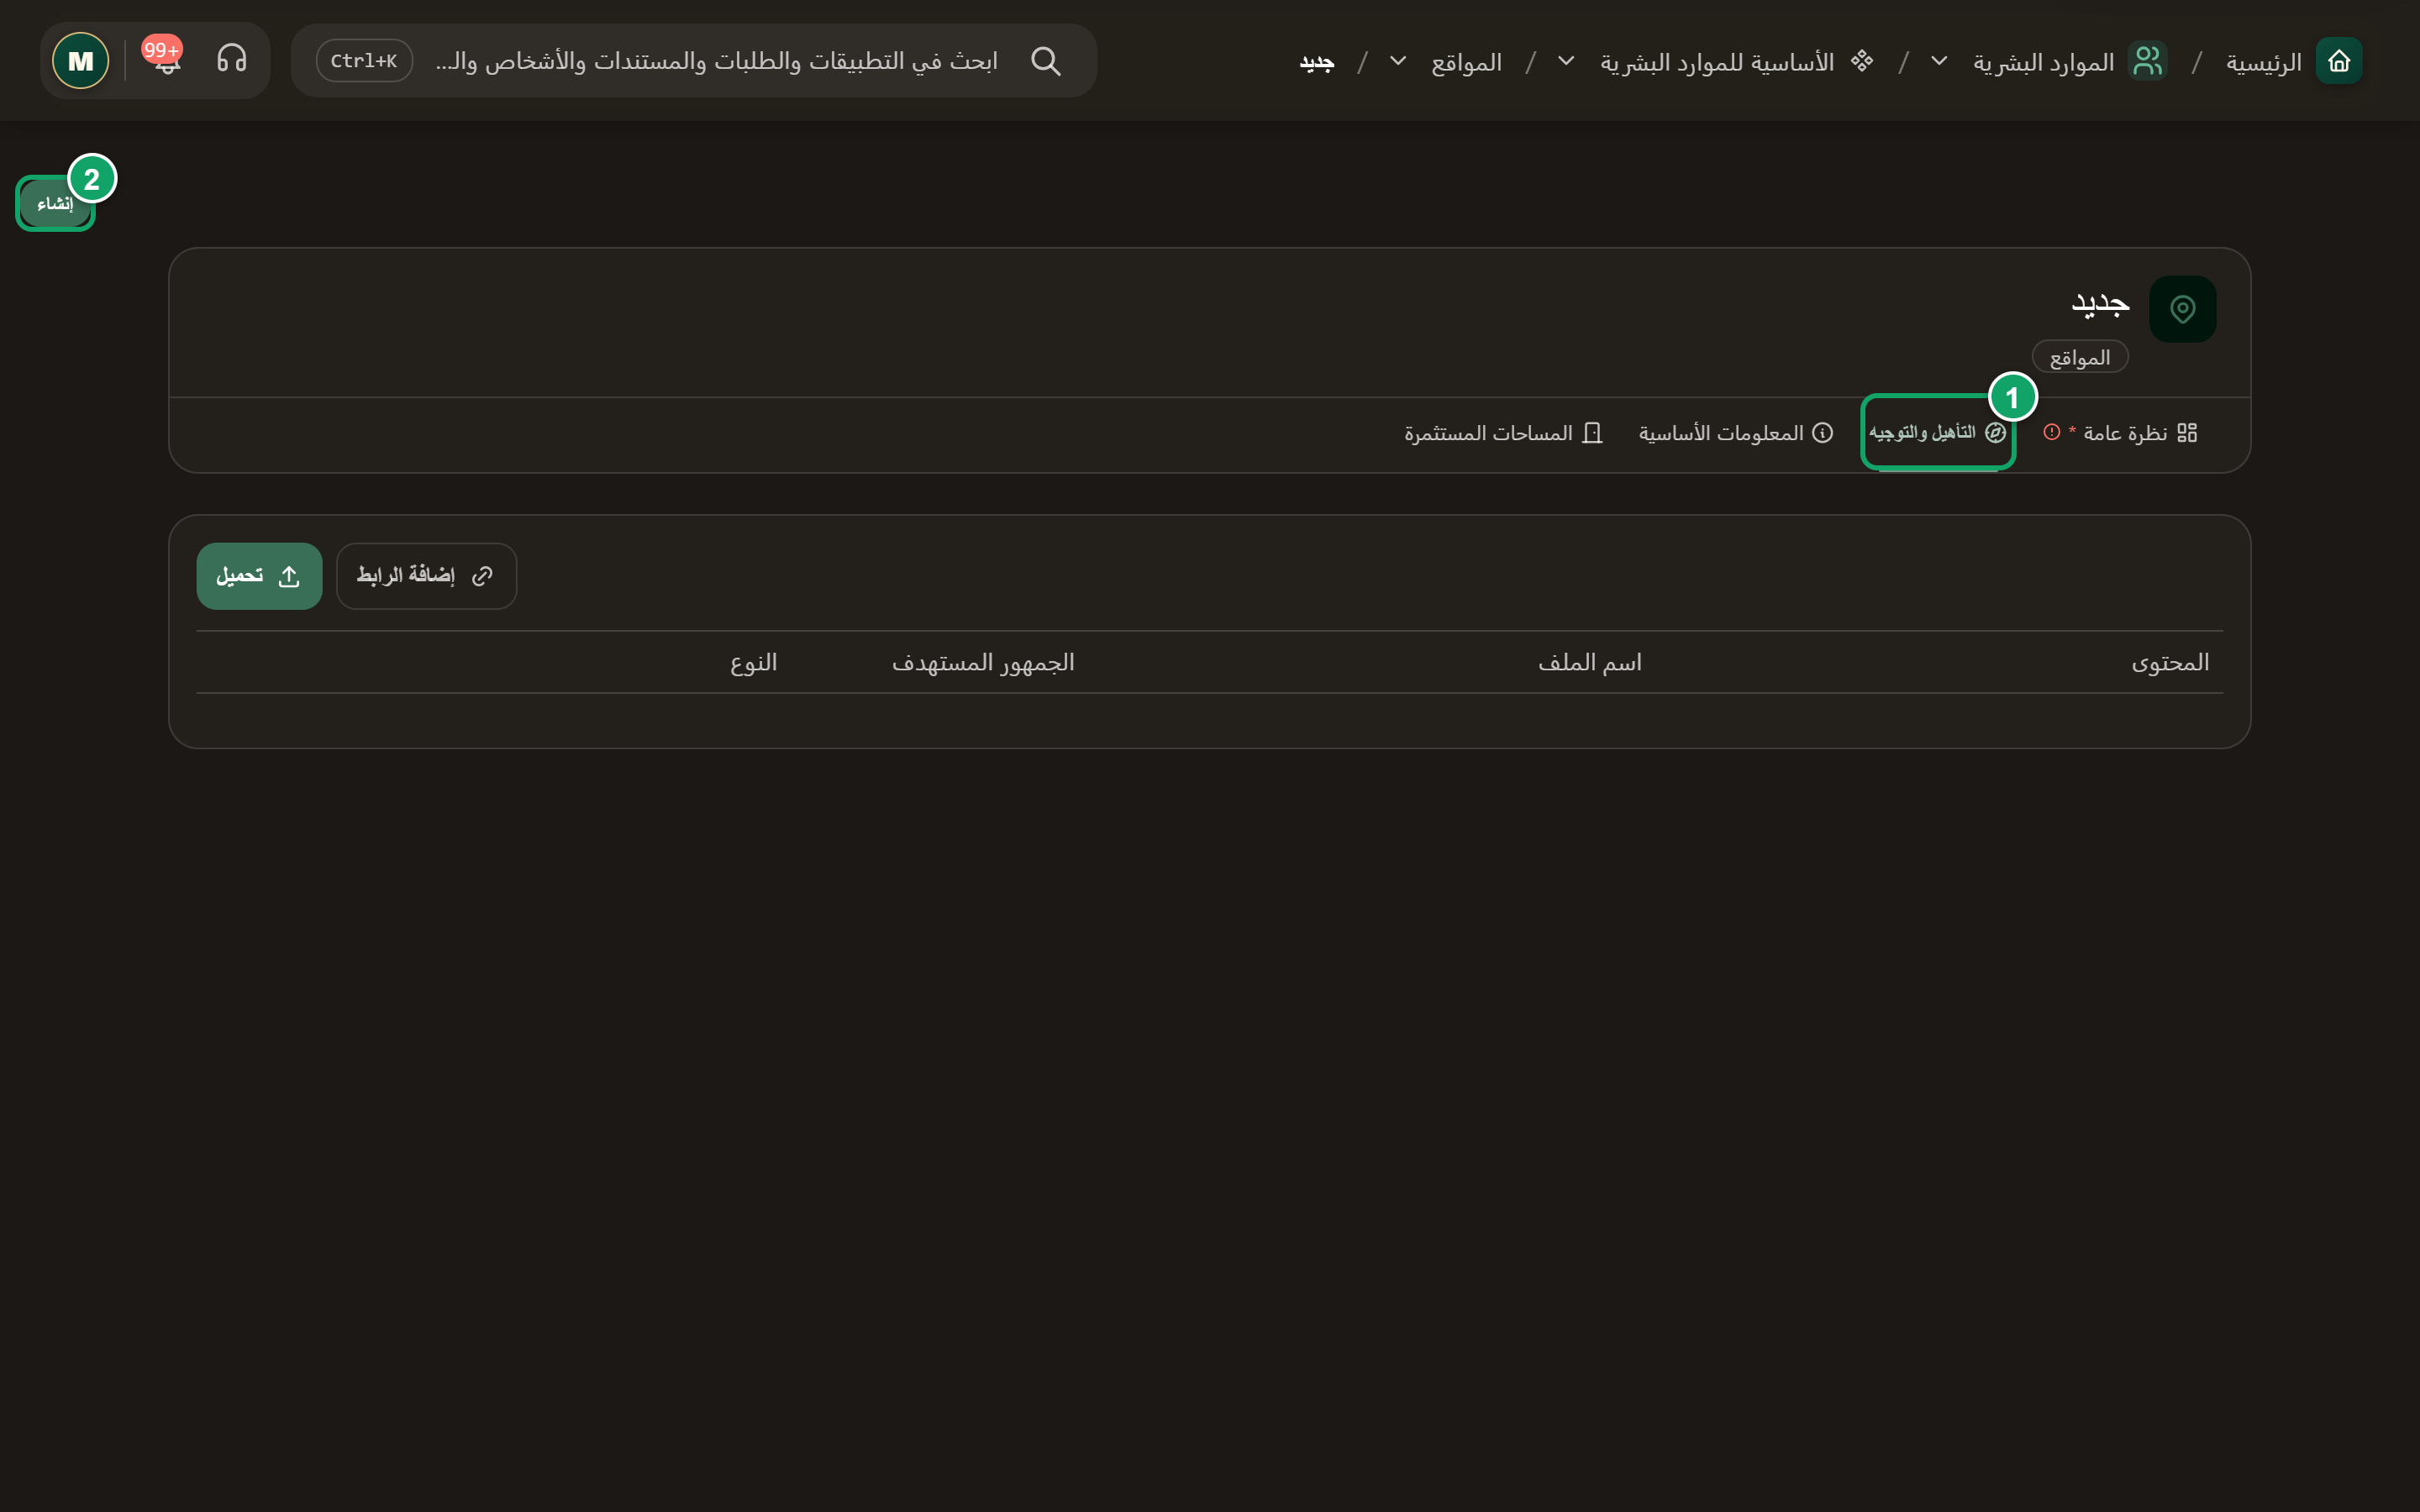
\includegraphics[width=0.95\linewidth]{figures/screens/ch02-location-fields-tab2-ar.png}
\caption{تبويب «التأهيل والتوجيه» كاملاً؛ نموذج غير محفوظ}
\label{fig:hr-locations-fulltab1}
\end{figure}

\begin{figure}[H]
\centering
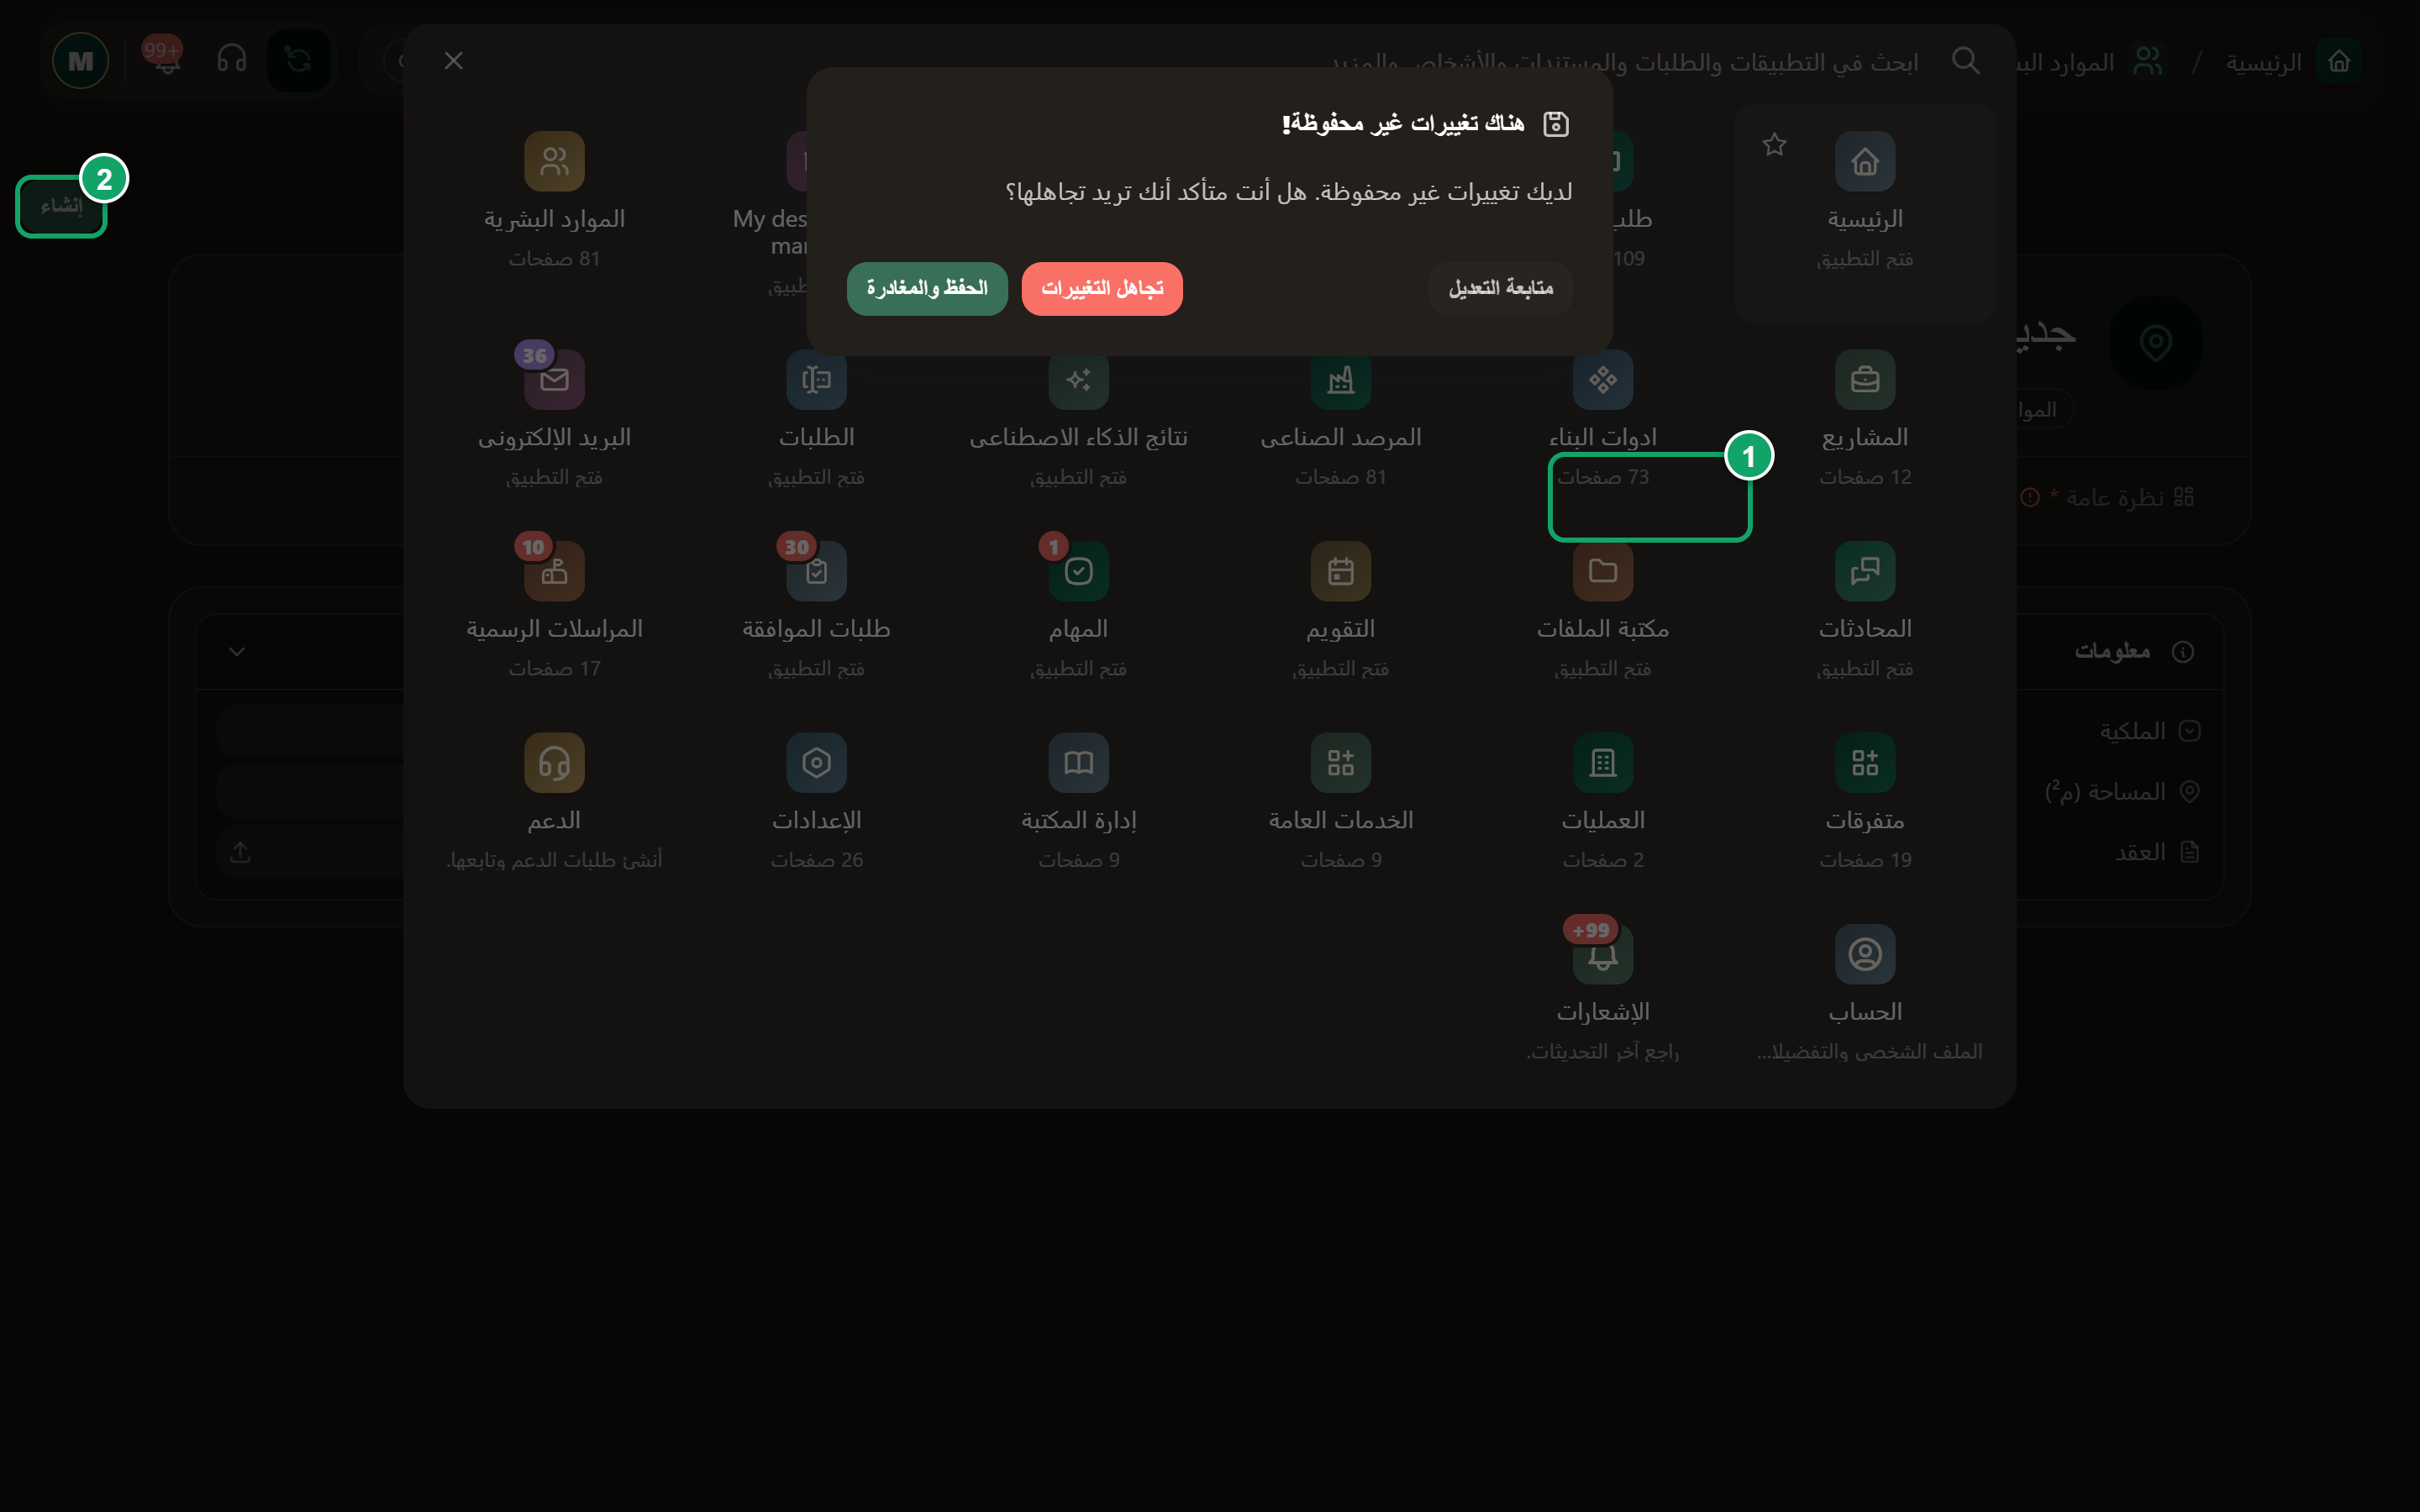
\includegraphics[width=0.95\linewidth]{figures/screens/ch02-location-fields-tab3-ar.png}
\caption{تبويب «المعلومات الأساسية» كاملاً؛ نموذج غير محفوظ}
\label{fig:hr-locations-fulltab2}
\end{figure}

\begin{figure}[H]
\centering
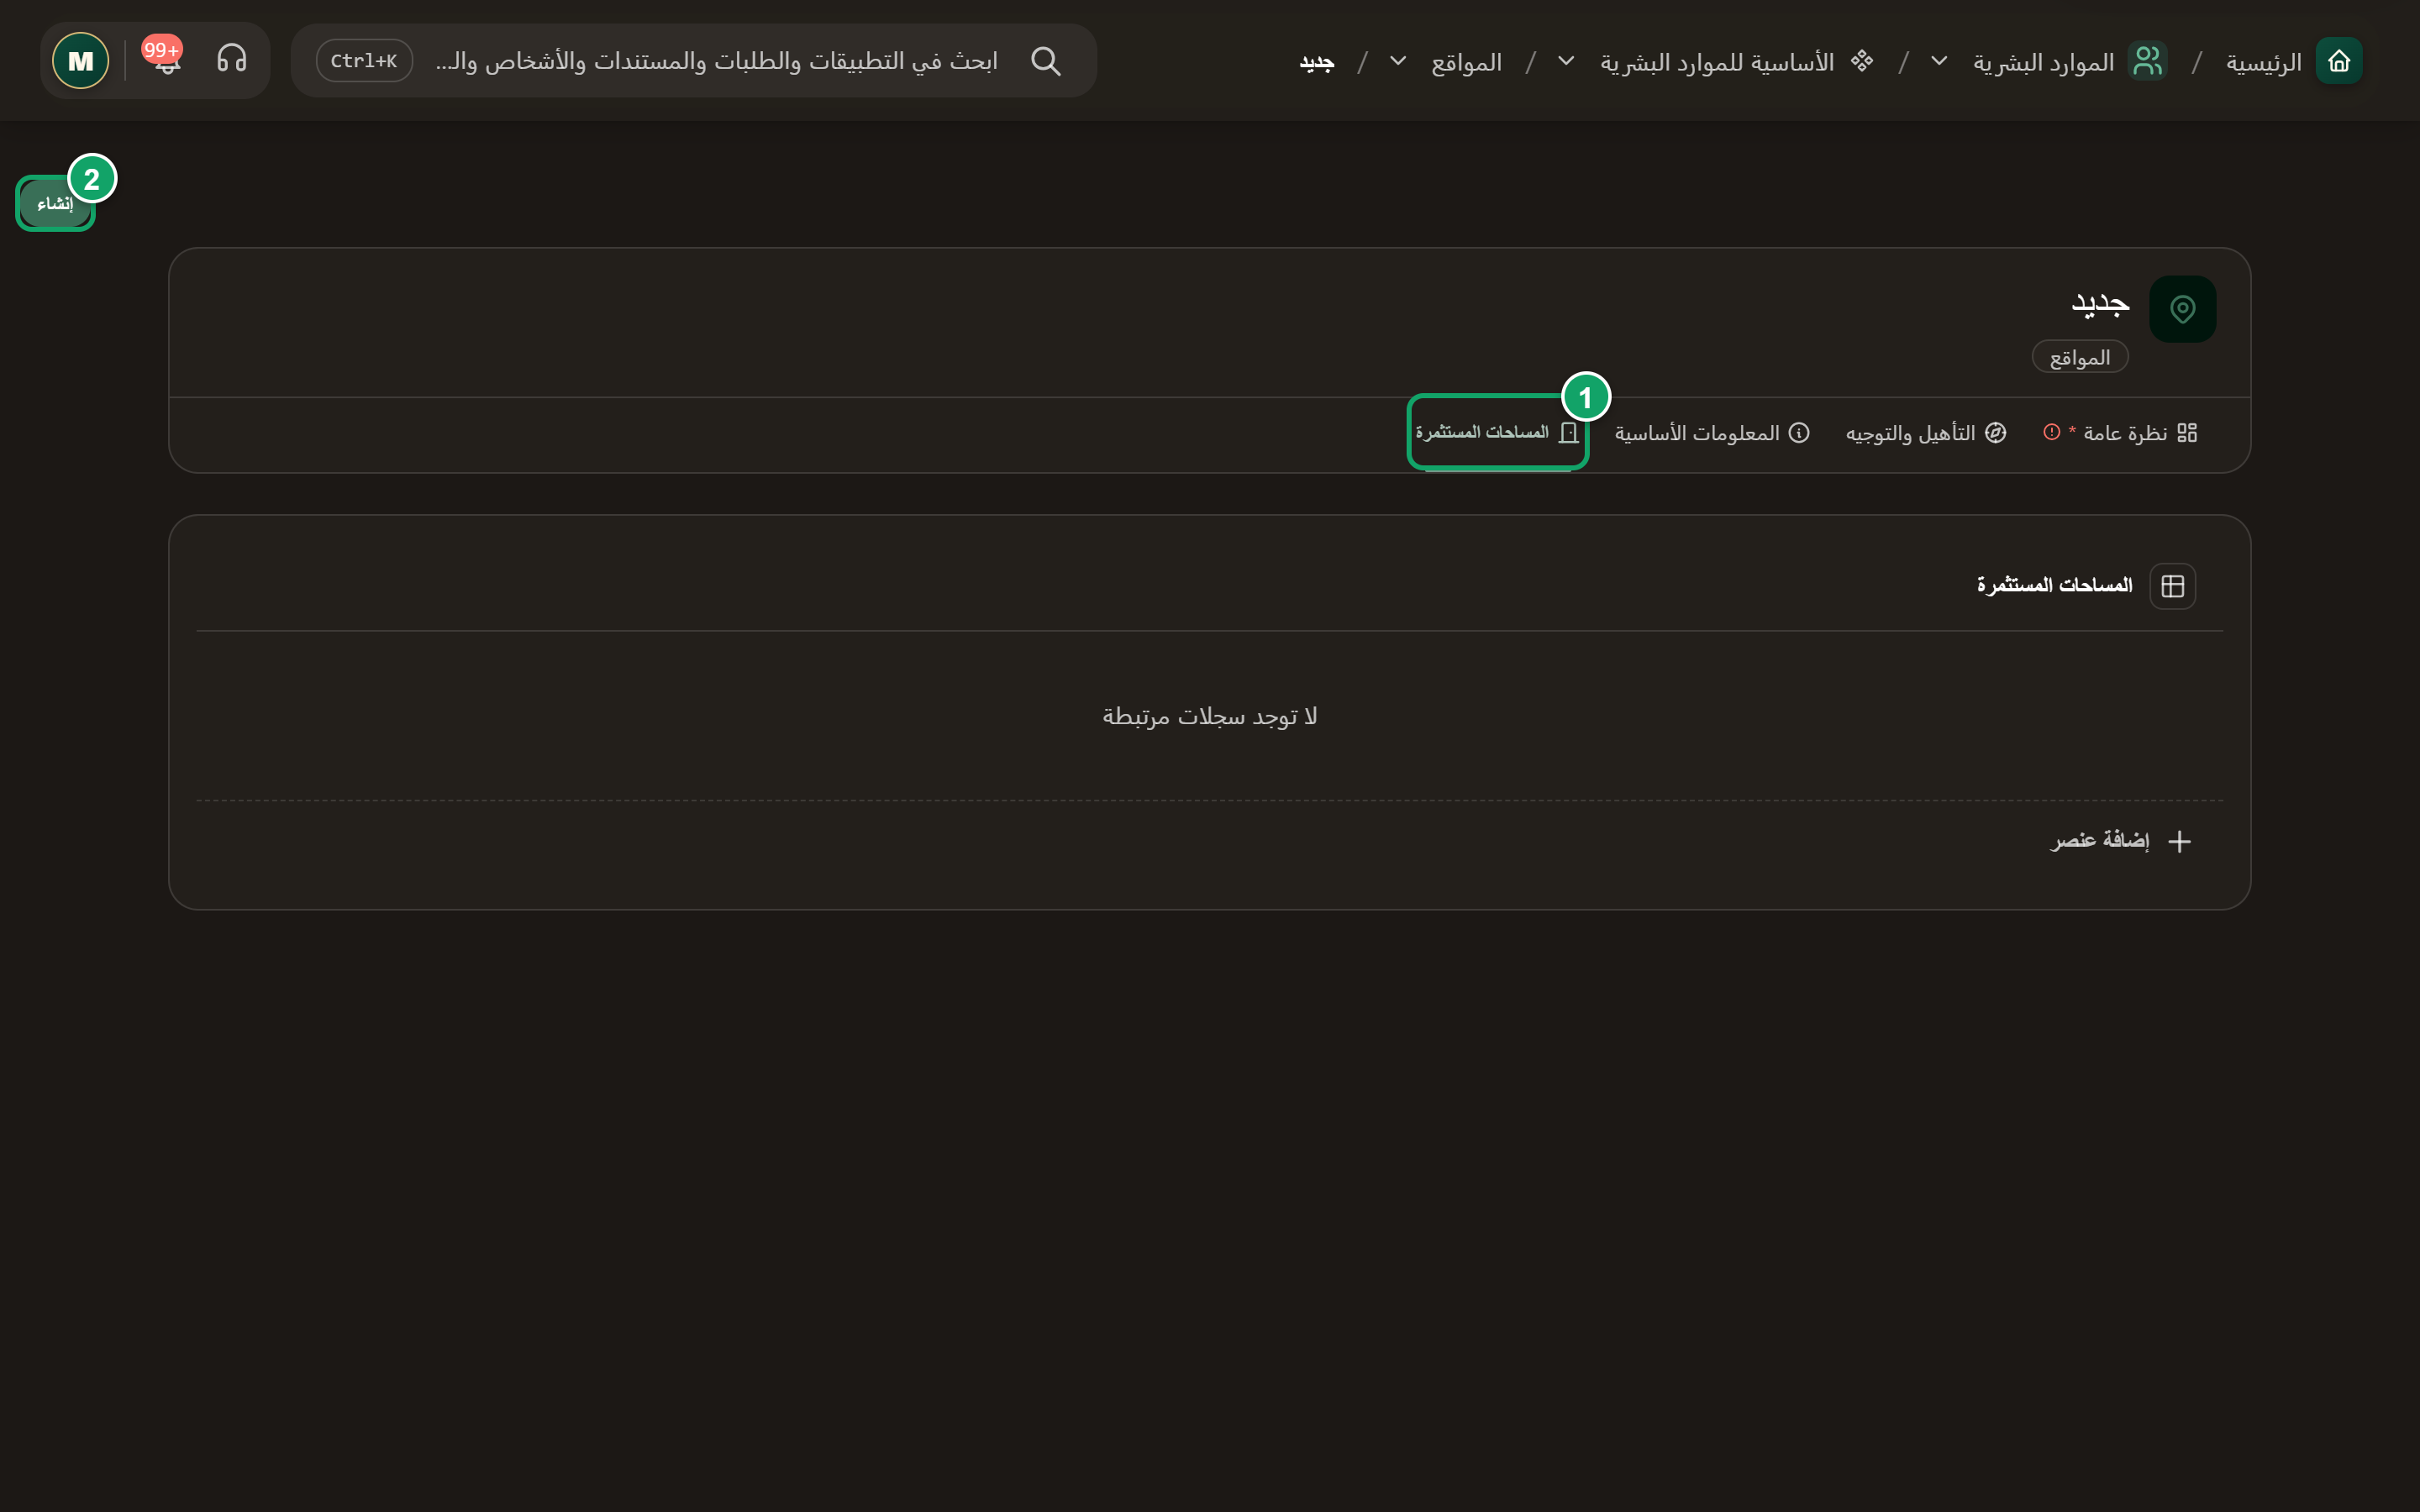
\includegraphics[width=0.95\linewidth]{figures/screens/ch02-location-fields-tab4-ar.png}
\caption{تبويب «المساحات المستثمرة» كاملاً؛ نموذج غير محفوظ}
\label{fig:hr-locations-fulltab3}
\end{figure}

\clearpage
\section{المجموعات}
\label{sec:hr-feature-groups}

المجموعة فريق أو لجنة تجمع أعضاء من أقسام مختلفة، دون تغيير وظائفهم.

\textbf{متى تفيد؟} مثلاً فريق تجهيز مكتب الأفق، أو لجنة تضم كل موظفي فرع حلب. \textbf{المسار:} «الموارد البشرية» / «القوى العاملة» / «المجموعات».

\begin{figure}[H]
\centering
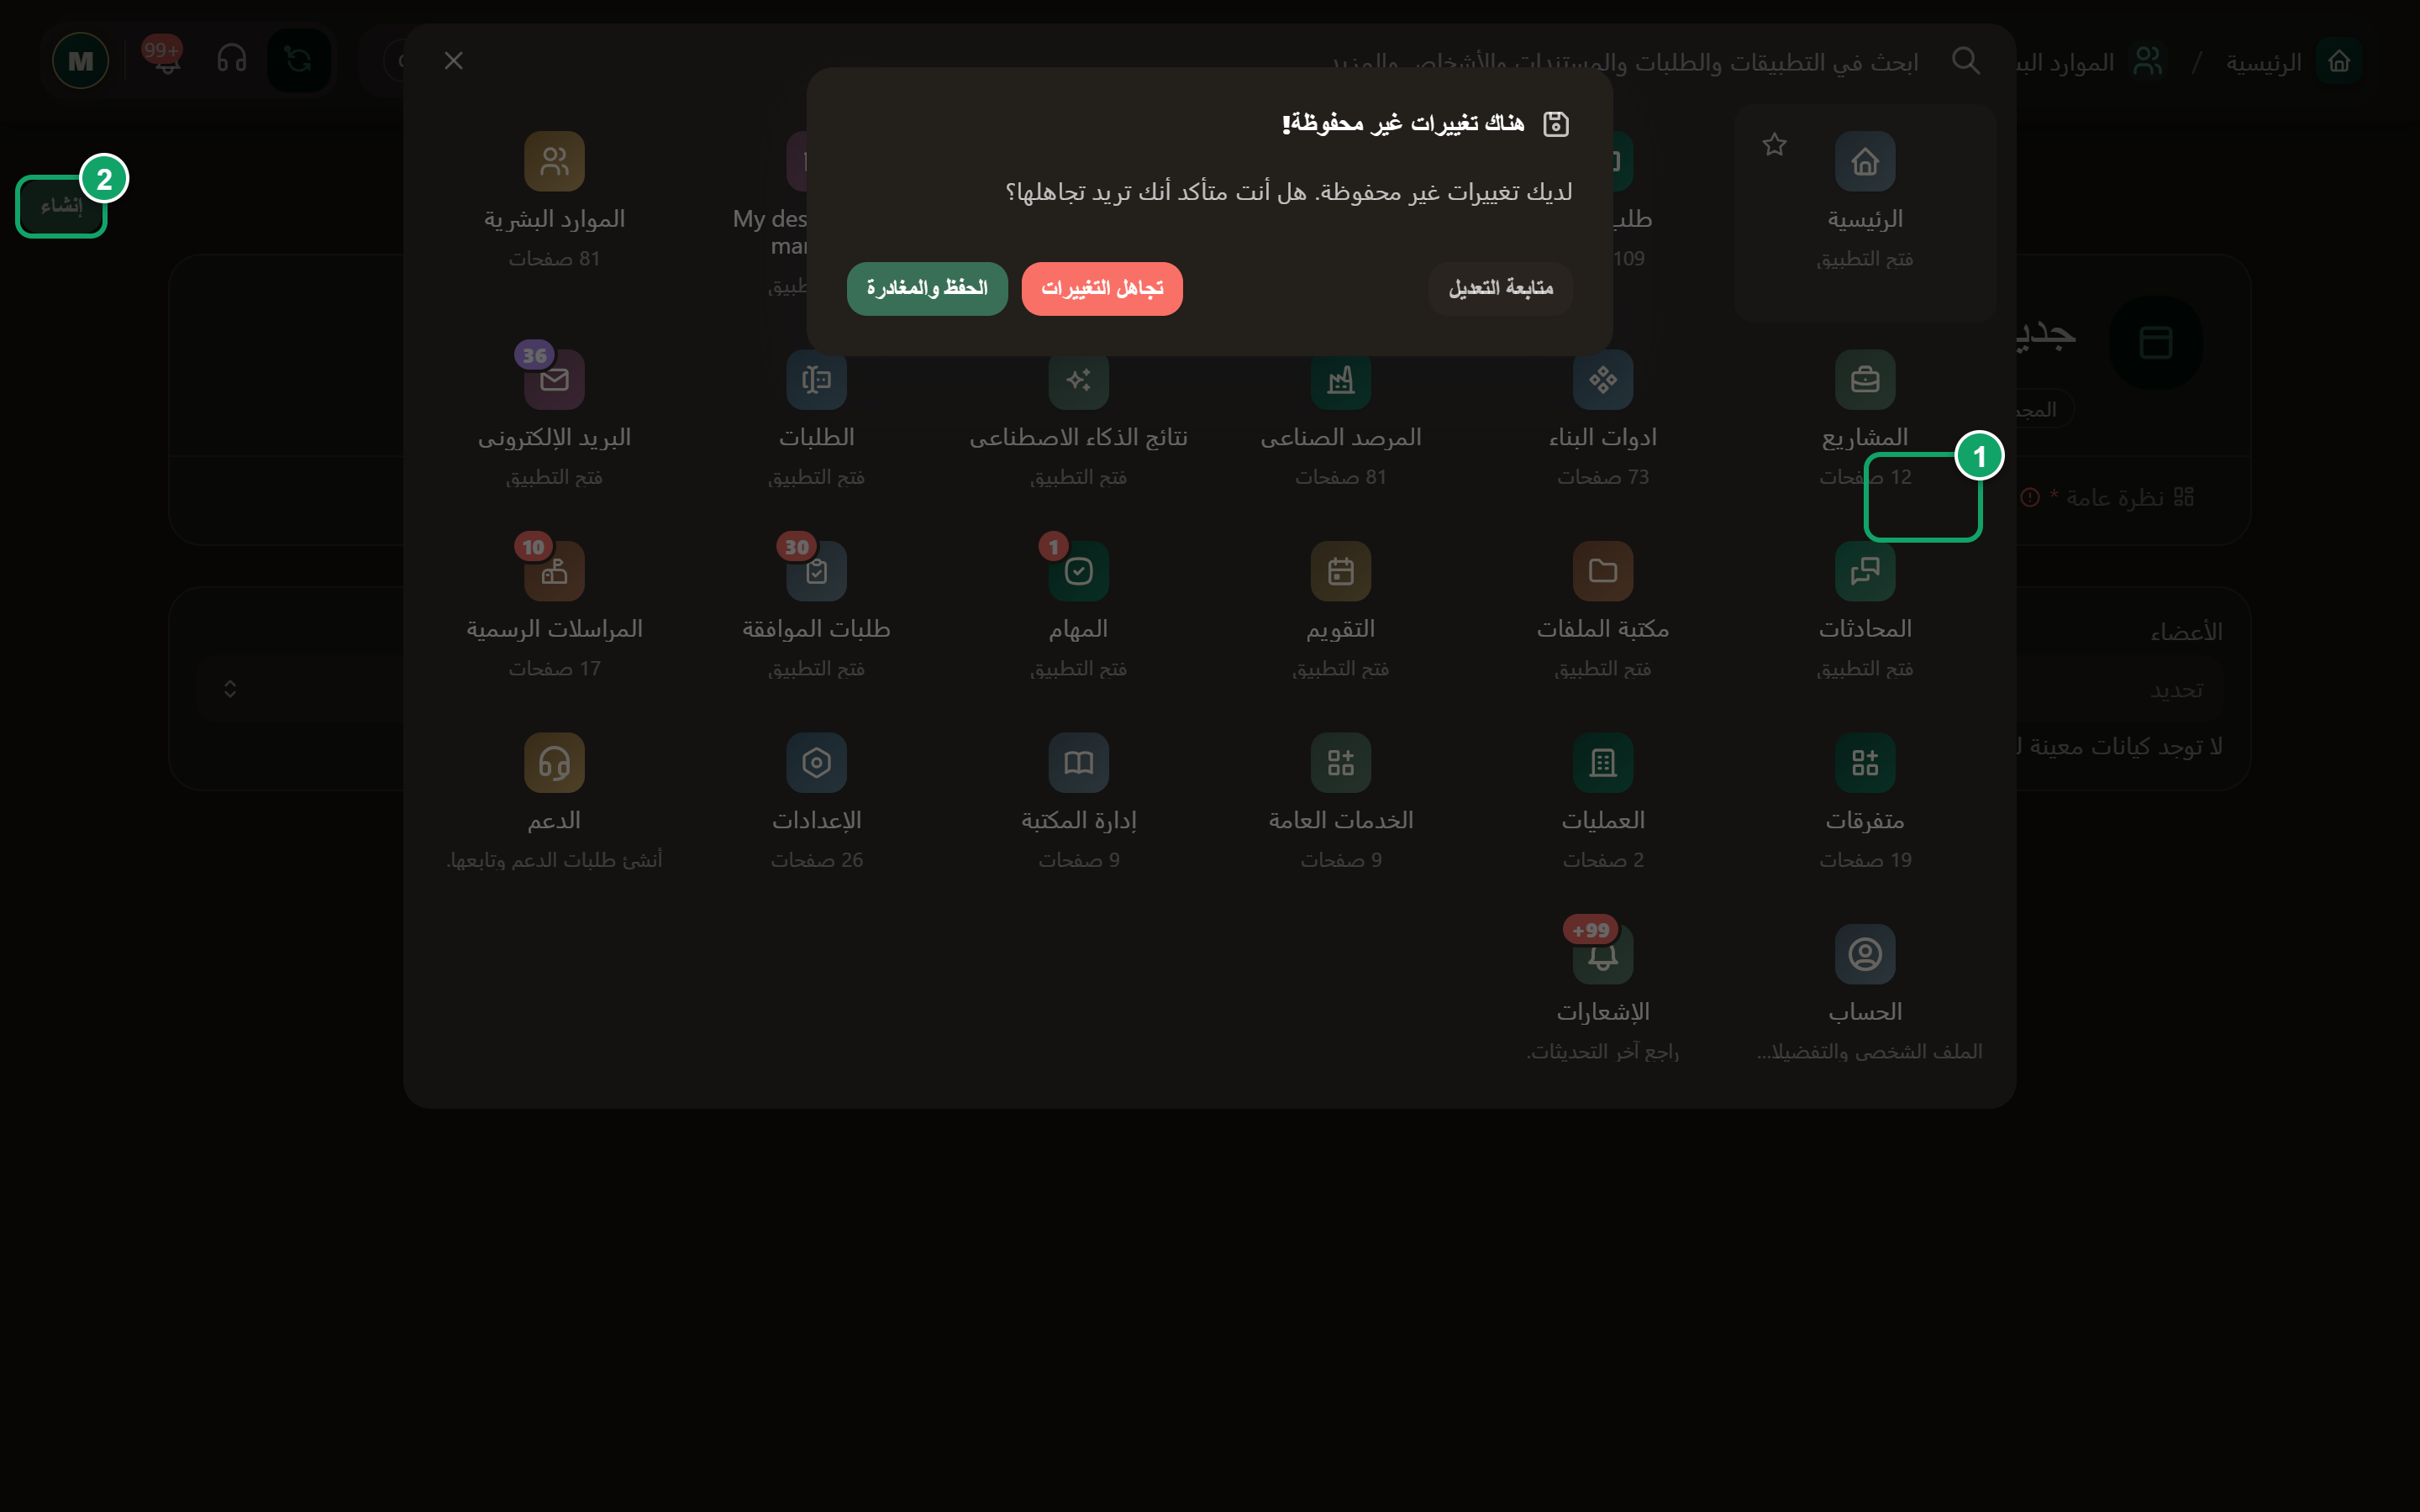
\includegraphics[width=0.95\linewidth]{figures/screens/ch03-feature-groups-ar.png}
\caption{المجموعات: نموذج غير محفوظ في بيئة الاختبار}
\label{fig:hr-feature-groups-screen}
\end{figure}

\begin{table}[H]
\centering
\caption{ما الذي تسجله في المجموعة؟}
\label{tab:hr-feature-groups-data}
\rcZebra
\begin{tabularx}{\linewidth}{R{3.6cm} Y}
\rcHeaderRow
\thh{التبويب أو الحقل} & \thh{ما الذي تضيفه؟}\\
الأساسية & الرمز والاسم \req{}، والوصف.\\
نوع المجموعة & \req{}: «يدوي» تختار أعضاءها بنفسك، أو «قائم على الكود» يحدد فيه شرطٌ الأعضاء ويحسبهم النظام \gen{}.\\
الأعضاء & أشخاص، أو كل من في قسم أو موقع أو منصب أو مجموعة، أو المؤسسة كلها.\\
حسابات البريد & صندوق بريد مشترك، أو قائمة بريدية للمجموعة.\\
\end{tabularx}
\end{table}

\begin{figure}[H]
\centering
\begin{tikzpicture}[node distance=0.5cm,stepBox/.append style={minimum width=6.5cm,text width=6.1cm,minimum height=0.8cm}]
  \node[stepBox] (a) {\RL{تحديد الفريق}};
  \node[stepBox,below=of a] (b) {\RL{اختيار طريقة العضوية}};
  \node[stepBox,below=of b] (c) {\RL{مراجعة الأعضاء}};
  \draw[flowsTo] (a) -- (b);
  \draw[flowsTo] (b) -- (c);
\end{tikzpicture}
\rclegend
\caption{خطوات الاستخدام؛ الأسهم لا تعني معالجة تلقائية}
\label{fig:hr-feature-groups-flow}
\end{figure}

\subsection{جرّب وراجع}

\begin{enumerate}
  \item افتح «المجموعات» وتأكد أن المجموعة غير موجودة.
  \item أضف رمزاً واسماً، واختر «يدوي»، ثم افتح «الأعضاء» واختر سارة وعمر، واحفظ.
\end{enumerate}

\textbf{تحقق:} أعد فتح المجموعة وراجع الأعضاء. انضمام سارة إلى المجموعة لا يغيّر تعيينها مديرةً للموارد البشرية.

\begin{figure}[H]
\centering
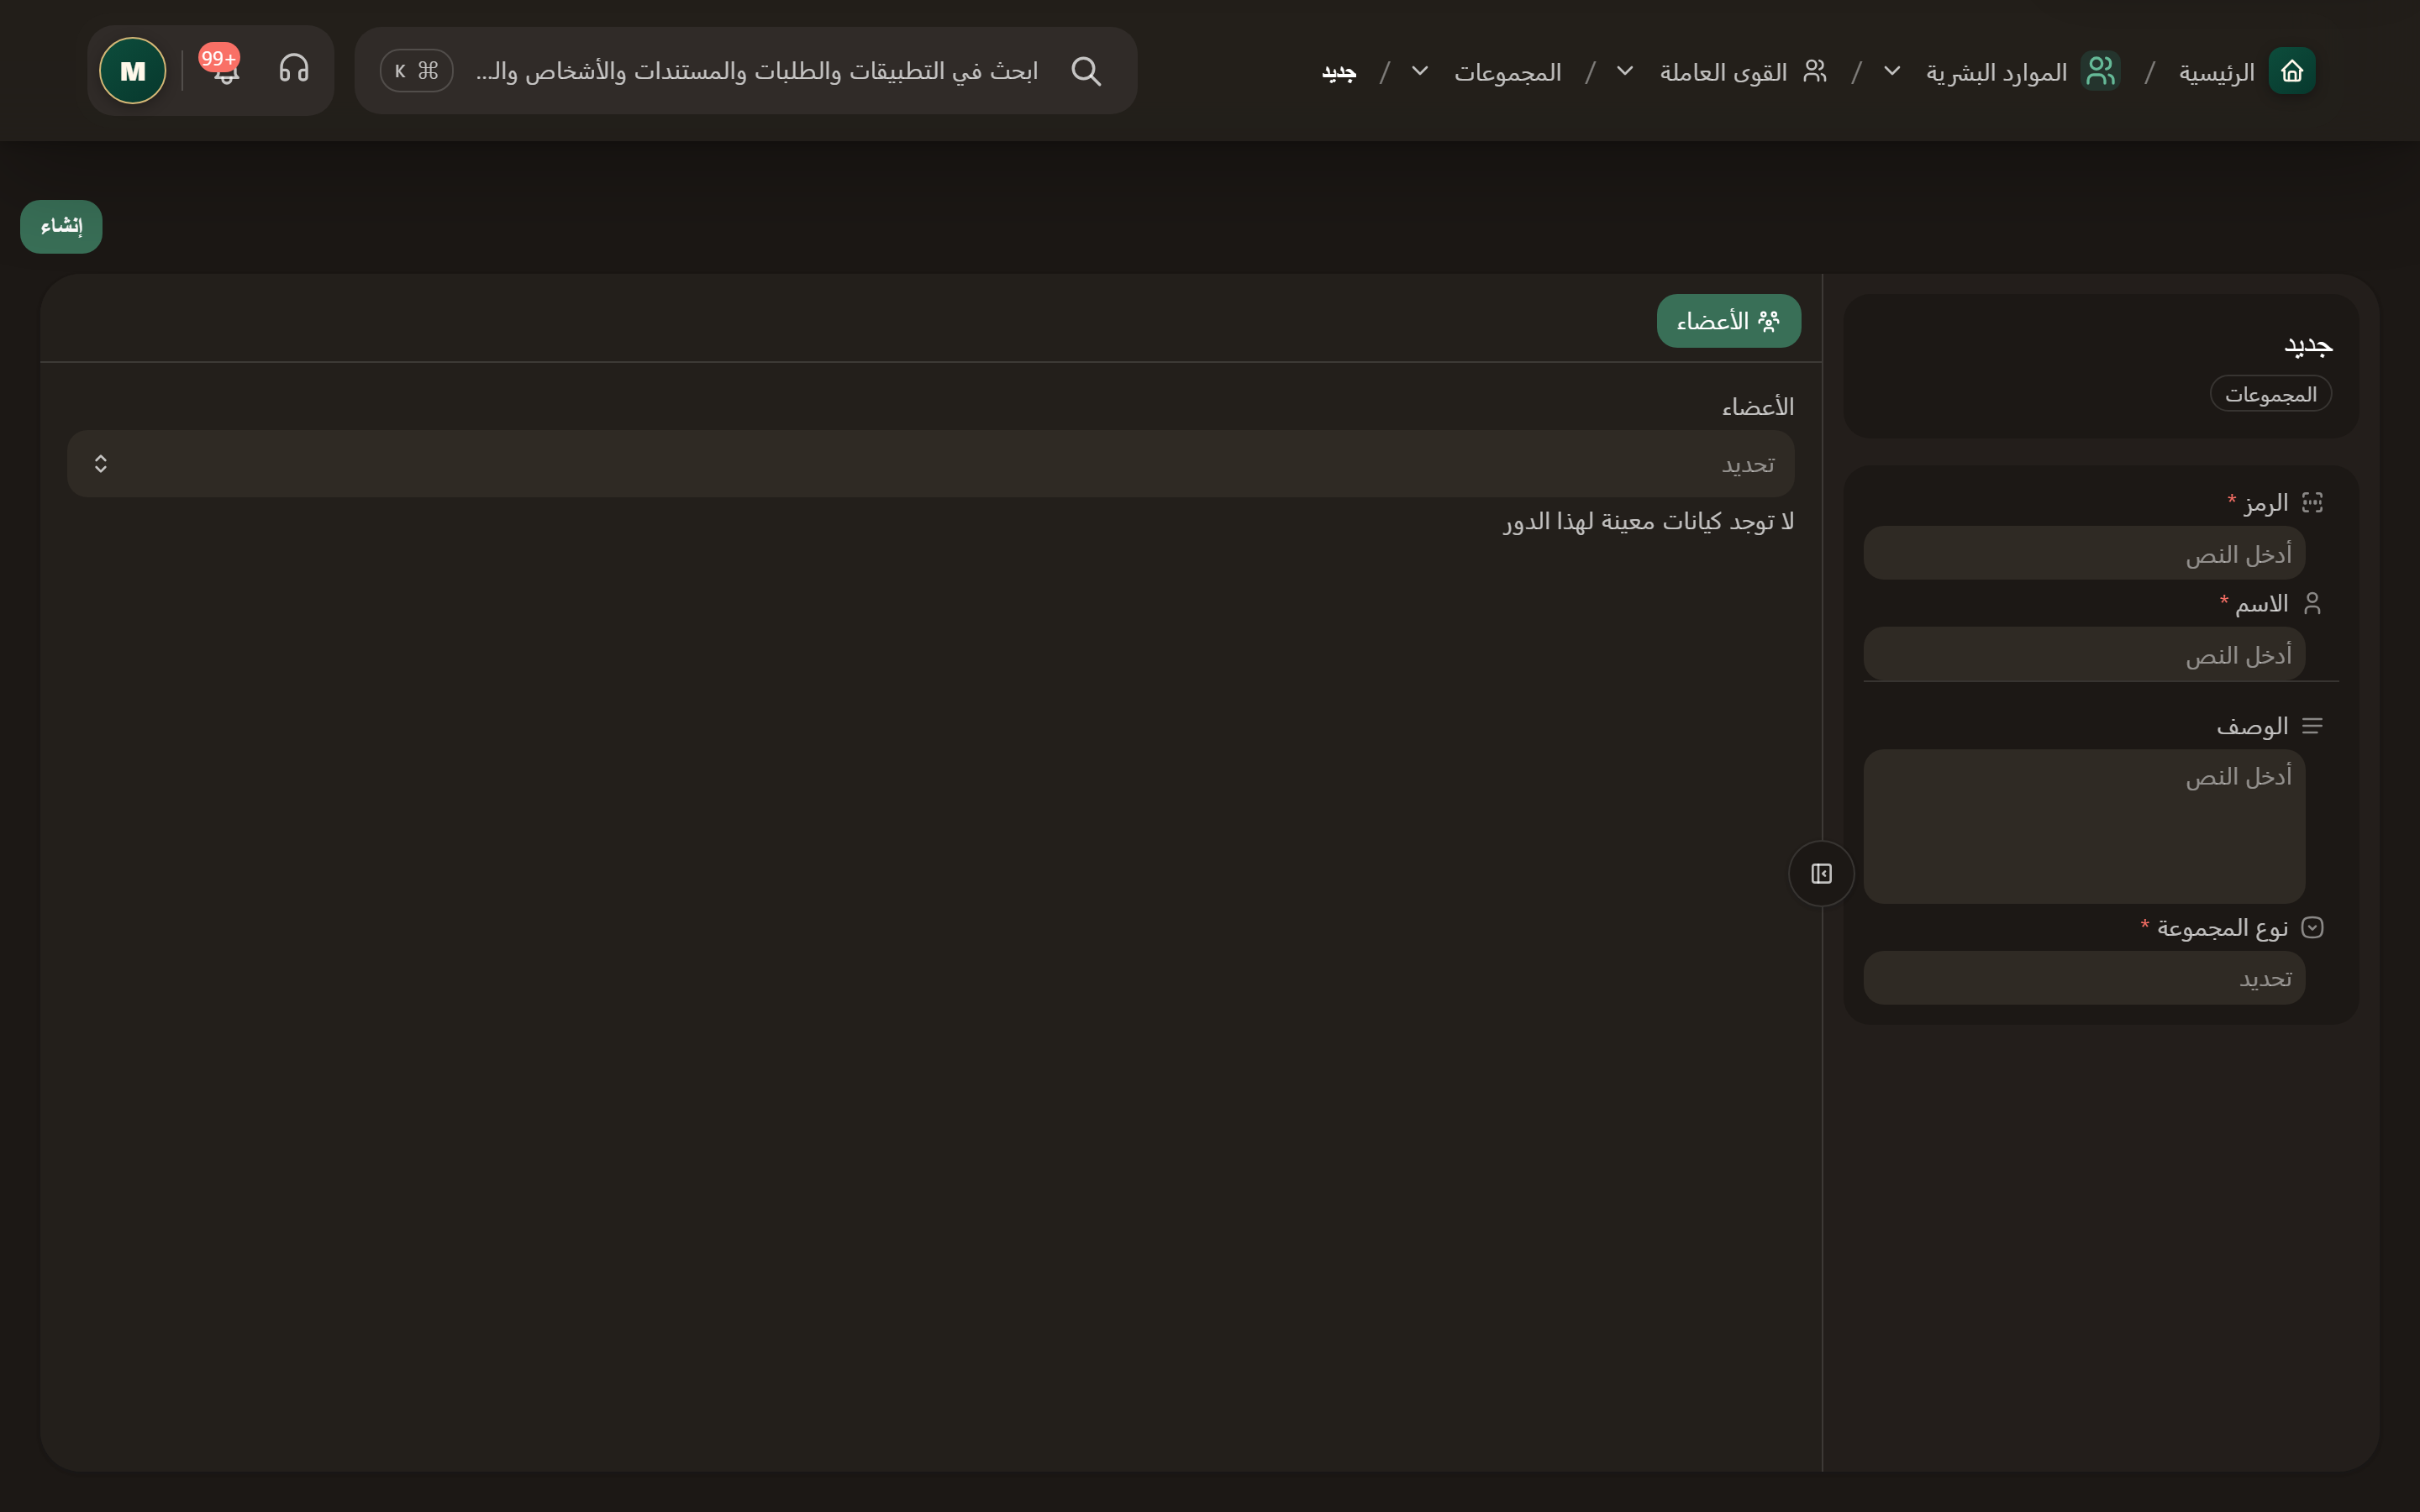
\includegraphics[width=0.95\linewidth]{figures/screens/ch03-feature-groups-tab1-ar.png}
\caption{تبويب «الأعضاء» كاملاً؛ نموذج غير محفوظ}
\label{fig:hr-groups-fulltab1}
\end{figure}

\clearpage
\section{الورديات}
\label{sec:hr-feature-shifts}

الوردية تحدد أيام العمل وساعاته واستراحاته المتوقعة. الحضور يسجل ما حدث فعلاً.

\textbf{متى تفيد؟} جدول واحد لكل من يعمل بالنمط نفسه، بدلاً من تكرار الأوقات لكل موظف. \textbf{المسار:} «الموارد البشرية» / «الوقت» / «الورديات».

\begin{figure}[H]
\centering
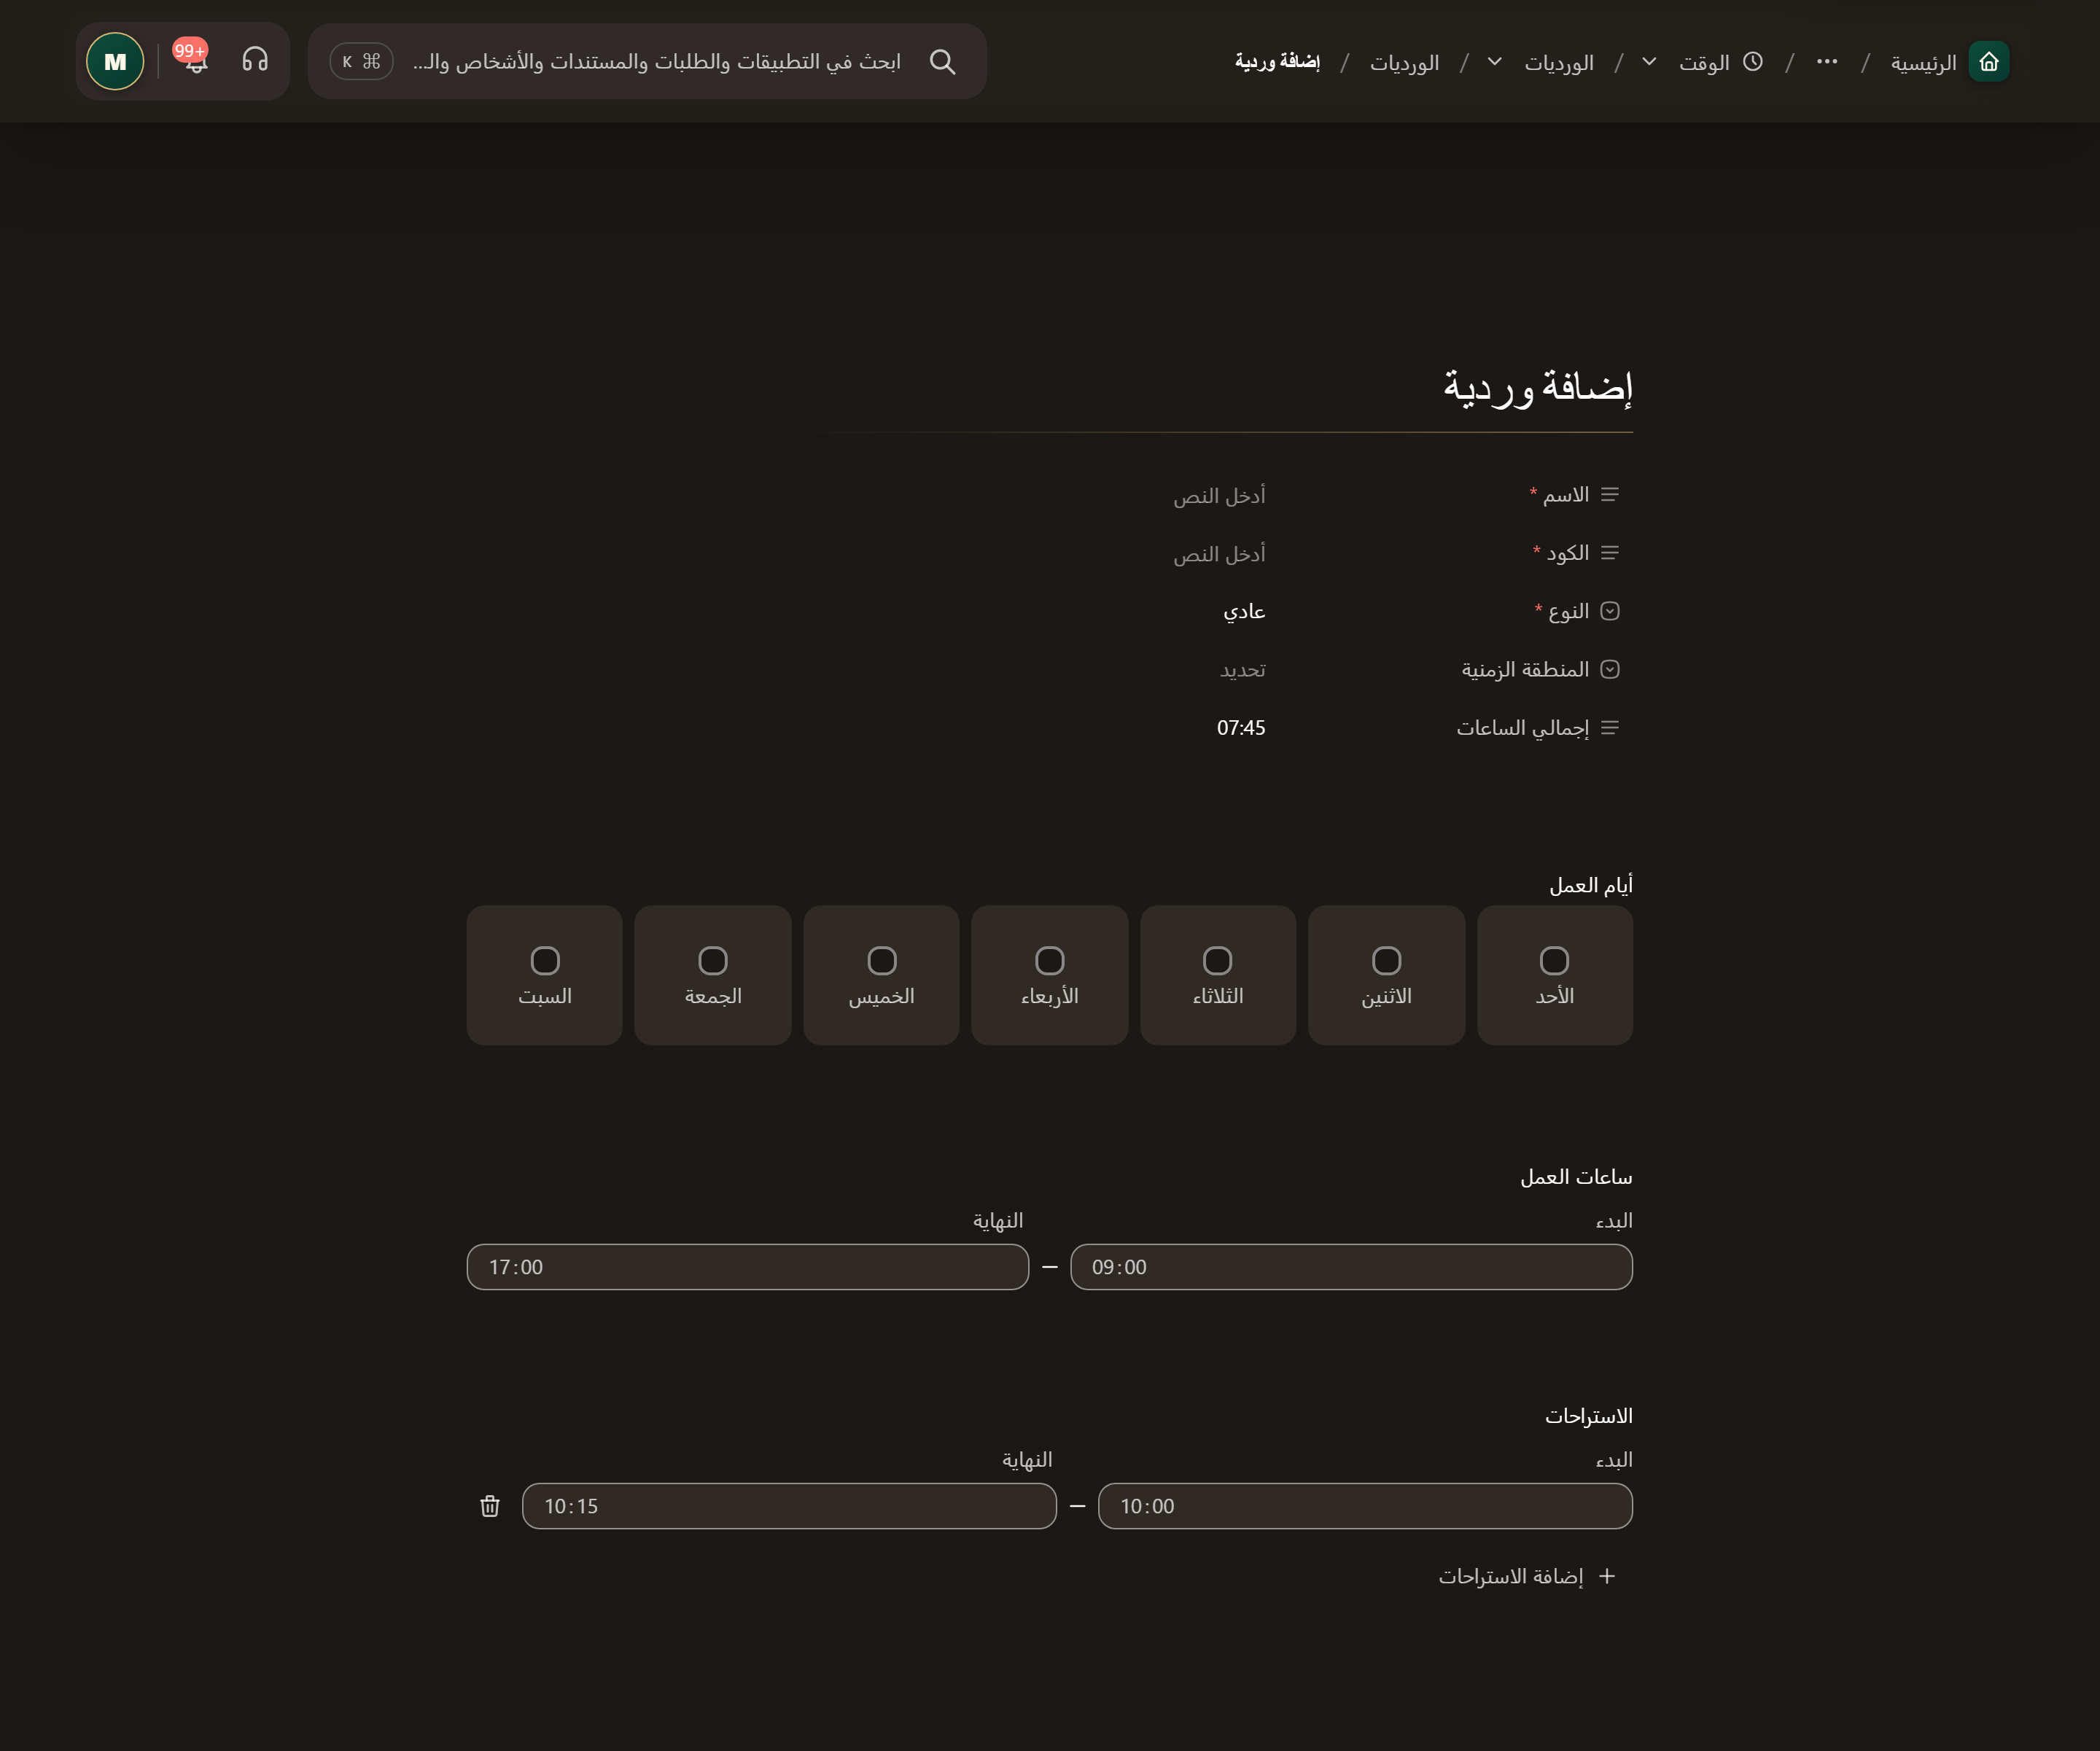
\includegraphics[width=0.95\linewidth]{figures/screens/ch03-shift-example-ar.png}
\caption{الورديات: نموذج الإضافة كاملاً؛ لم يُحفظ}
\label{fig:hr-feature-shifts-screen}
\end{figure}

\begin{table}[H]
\centering
\caption{اختيار نوع الوردية}
\label{tab:hr-shift-types}
\rcZebra
\begin{tabularx}{\linewidth}{R{2.4cm} Y Y}
\rcHeaderRow
\thh{النوع} & \thh{ماذا تُدخل؟} & \thh{مثال توضيحي}\\
عادي & فترة عمل واحدة، واستراحات عند الحاجة. & من \en{09:00} إلى \en{17:00}.\\
مقسم & أكثر من فترة عمل، دون تداخل. & من \en{09:00} إلى \en{13:00}، ثم من \en{16:00} إلى \en{20:00}.\\
مرن & مدة العمل بالساعات والدقائق. & مدة \en{08:00} دون وقت بدء أو انتهاء.\\
ماراثون & مدة العمل بالساعات والدقائق. & لا تستنتج من الاسم وحده نظام عمل وراحة معيناً.\\
\end{tabularx}
\end{table}

\begin{table}[H]
\centering
\caption{ما الذي تسجله في الوردية؟}
\label{tab:hr-feature-shifts-data}
\rcZebra
\begin{tabularx}{\linewidth}{R{3.6cm} Y}
\rcHeaderRow
\thh{الحقل} & \thh{ما الذي تضيفه؟}\\
الاسم والرمز والنوع & \req{}؛ الرمز لا يتكرر.\\
أيام العمل & \req{}: اختر يوماً واحداً على الأقل من أيام الأسبوع.\\
المنطقة الزمنية & مثل \en{Asia/Damascus} \opt{}.\\
ساعات العمل والاستراحات & للنوعين العادي والمقسم؛ وتقع الاستراحة داخل ساعات العمل \opt{}.\\
المدة & للمرن والماراثون؛ لا يمكن أن تكون \en{00:00}.\\
إجمالي الساعات & ساعات العمل بعد طرح الاستراحات \gen{}.\\
\end{tabularx}
\end{table}

\subsection{أنشئ الوردية خطوة بخطوة}
\label{sec:hr-shifts}

\begin{enumerate}
  \item افتح «الورديات» وأضف «الدوام الإداري»، الرمز \en{HZN-S-01}، النوع «عادي».
  \item اختر الأحد إلى الخميس، والمنطقة الزمنية \en{Asia/Damascus}.
  \item ساعات العمل: \en{09:00–17:00}. عدّل الاستراحة الموجودة إلى \en{13:00–13:30}؛ لا تضف استراحة ثانية.
  \item تحقق من الإجمالي \en{07:30}، ثم «حفظ». أعد فتح الوردية وتحقق من القيم.
\end{enumerate}

\begin{rcnote}[تجنب خطأ الوقت]
لا تجعل الفترات تتداخل، واجعل الاستراحة داخل ساعات العمل. \en{22:00–06:00} تنتهي في اليوم التالي. لا يُسمح بتساوي وقت البدء ووقت النهاية.
\end{rcnote}

\subsection{كيف تصل الوردية إلى الموظف؟}
\label{sec:hr-shift-inheritance}

وراثة الوردية تعني استخدام وردية المنصب أو القسم أو الموقع عندما لا تُحدد وردية خاصة للتعيين.

\begin{figure}[H]
\centering
\begin{tikzpicture}[node distance=0.4cm,stepBox/.append style={minimum width=6.5cm,text width=6.1cm,minimum height=0.7cm}]
  \node[stepBox] (a) {\RL{وردية التعيين}};
  \node[stepBox,below=of a] (p) {\RL{وردية المنصب}};
  \node[stepBox,below=of p] (n) {\RL{وردية الوحدة، ثم}\\\RL{وحداتها الأم}};
  \node[stepBox,below=of n] (l) {\RL{وردية الموقع، ثم}\\\RL{مواقعه الأم}};
  \draw[flowsTo] (a) -- (p);
  \draw[flowsTo] (p) -- (n);
  \draw[flowsTo] (n) -- (l);
\end{tikzpicture}
\rclegend
\caption{ترتيب البحث عن الوردية: ينتقل النظام إلى المستوى التالي إذا لم يجد وردية}
\label{fig:hr-shift-order}
\end{figure}

يعتمد النظام أول وردية يجدها، ولا يجمع الورديات.

\begin{enumerate}
  \item افتح «الوحدات التنظيمية» / \en{HZN-HR}. اختر «تجاوز» أولاً عند الحاجة، ثم «الدوام الإداري» في «الوردية»، واحفظ.
  \item افتح «المناصب» / مدير الموارد البشرية، وتحقق من القسم والوردية.
  \item افتح تعيين سارة وتحقق من الوردية. إن اختلفت، راجع التعيين ثم المنصب حسب المخطط.
\end{enumerate}

\textbf{تحقق:} الوردية الصحيحة تظهر في تعيين سارة. «إعادة تعيين» تعيد الوراثة. لا تُحفظ الوردية؟ راجع الاسم والرمز والأيام والفترات المتداخلة. المدة أقل من المتوقع؟ لأن الاستراحات تُطرح منها. لا تُحذف؟ لأنها مستخدمة في تعيينات أو مناصب أو سجلات حضور.

\clearpage
\section{حضوري}
\label{sec:hr-feature-my-attendance}

تعرض صفحة «حضوري» حضورك الشهري كما احتسبه النظام: أيام العمل والعطل، ولكل يوم بصماته وإجمالياته وأثره في الراتب.

\textbf{متى تفيد؟} افهم يومك قبل طلب تصحيح. اليوم الفارغ لا يثبت الغياب؛ افحص مصدر البصمات أولاً. \textbf{المسار:} «الموارد البشرية» / «الوقت» / «حضوري».

\begin{figure}[H]
\centering
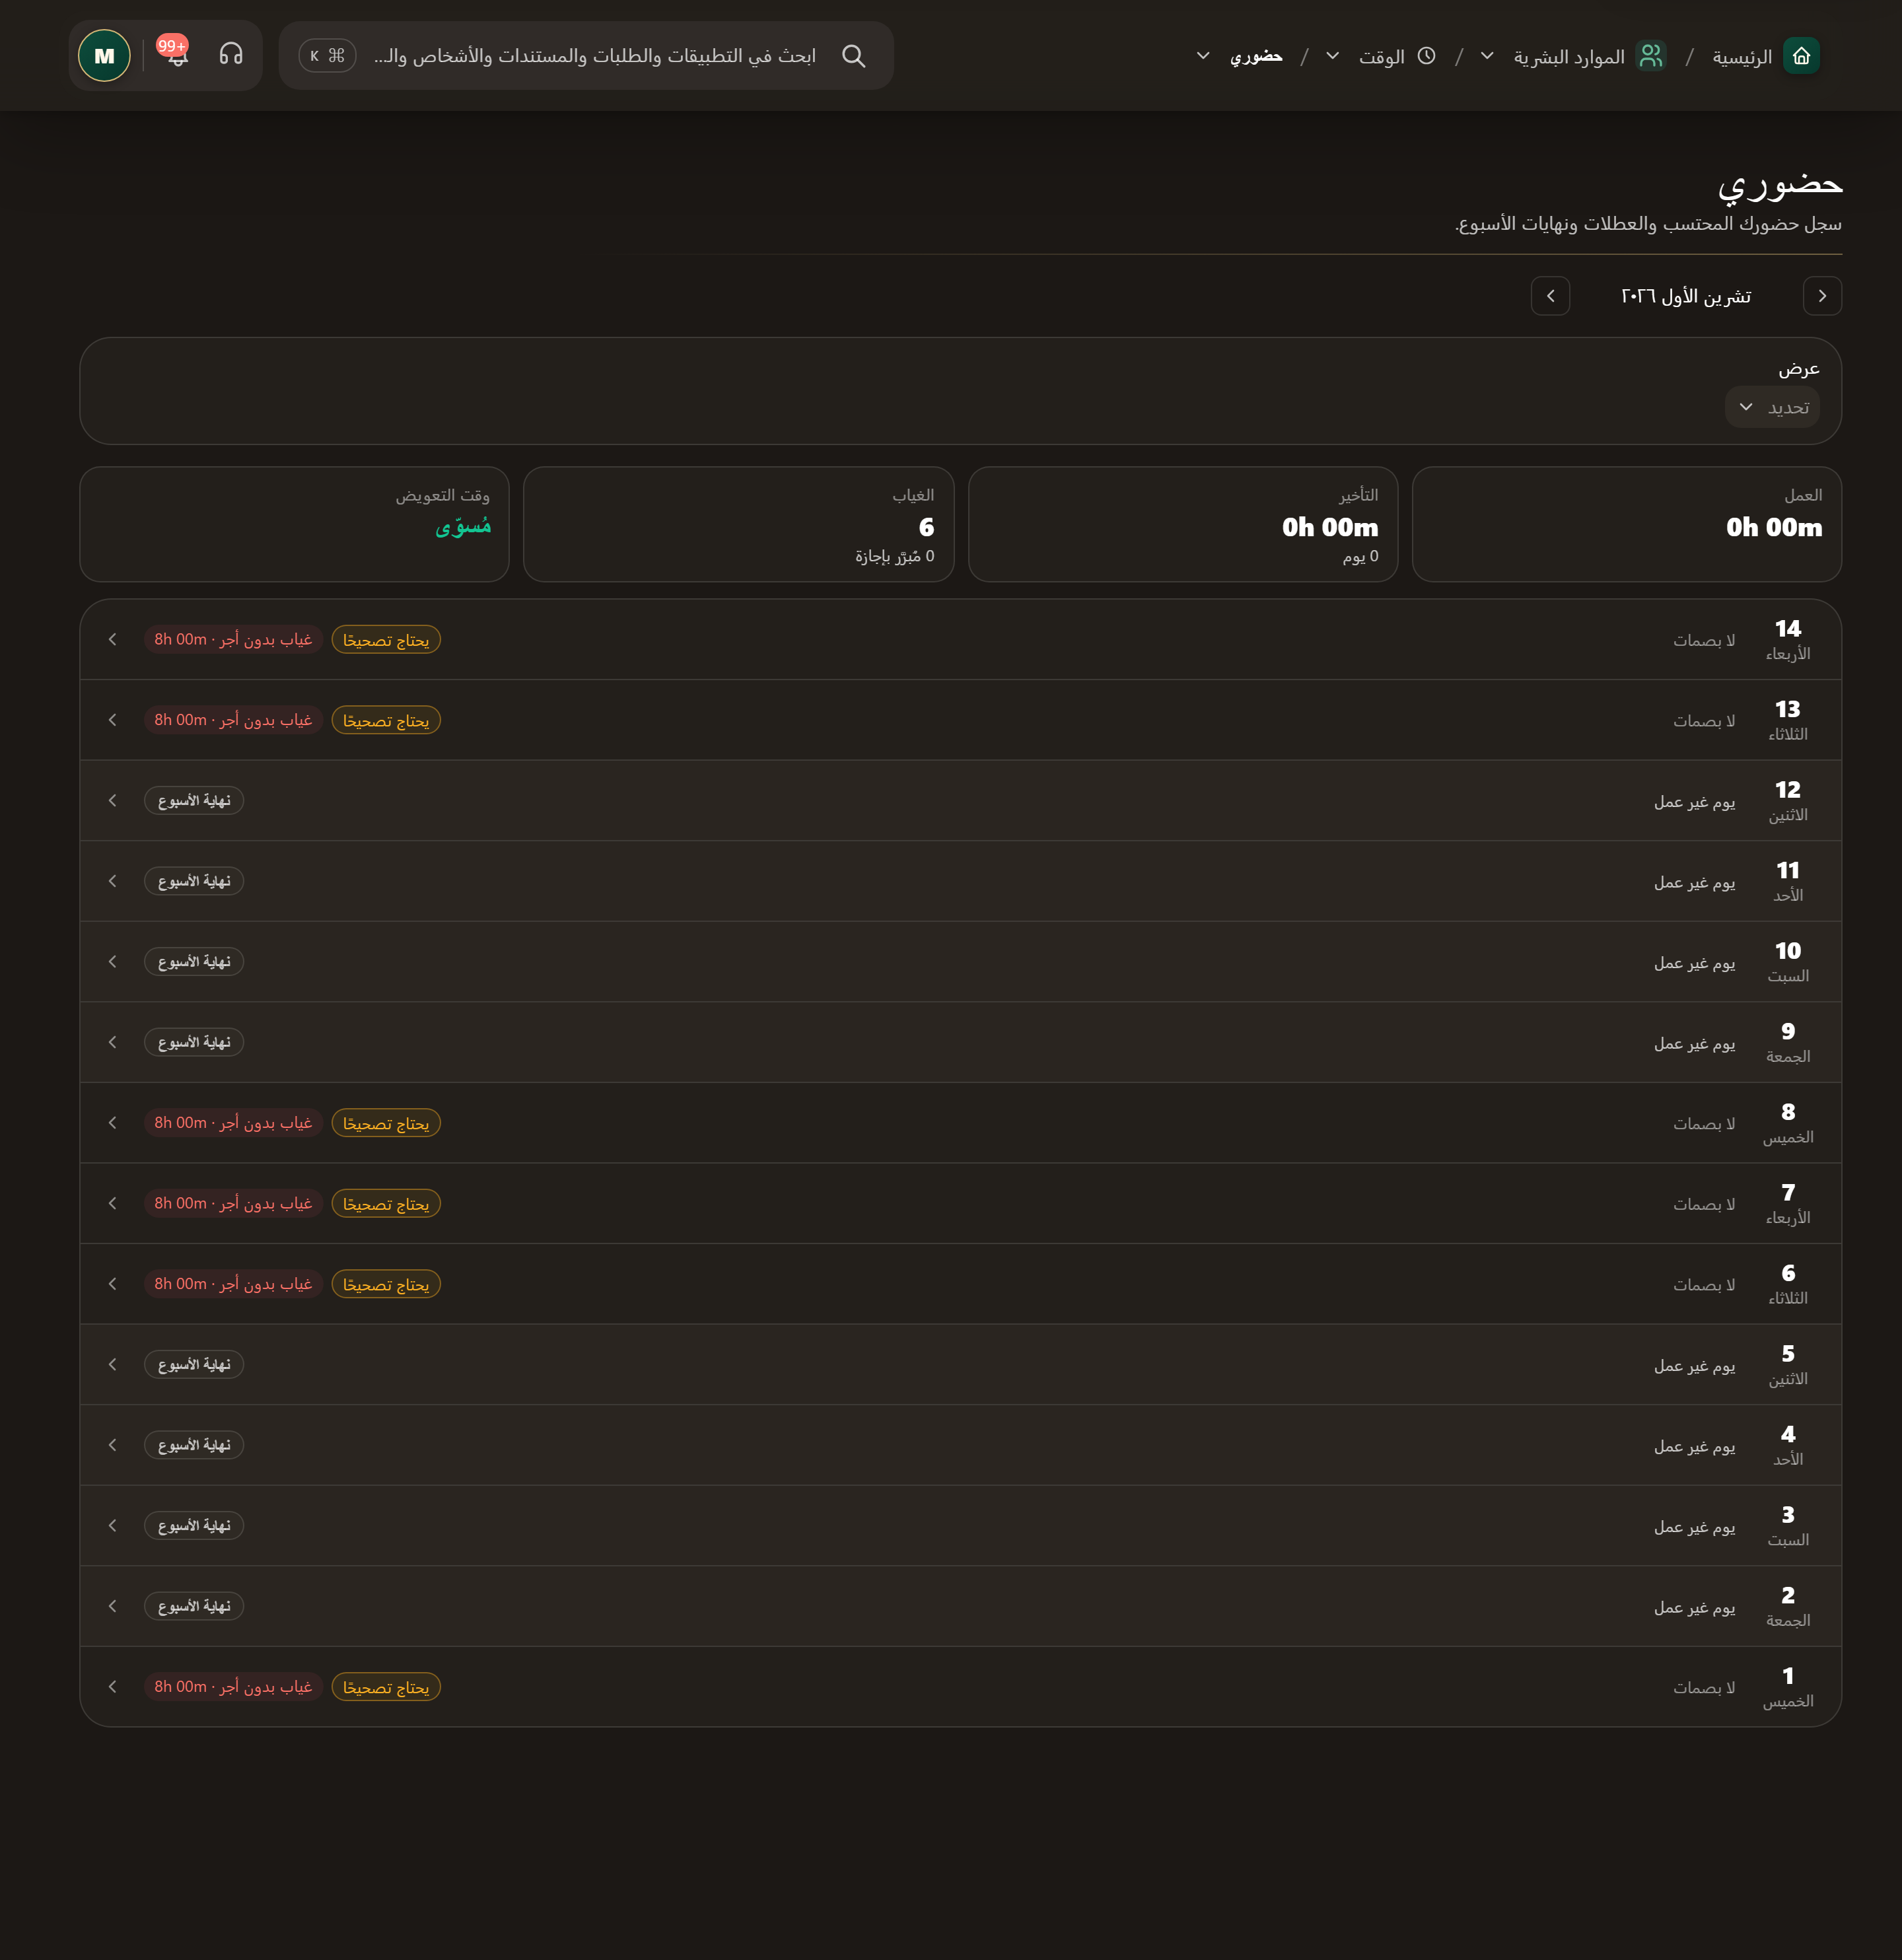
\includegraphics[width=0.95\linewidth]{figures/screens/ch03-feature-my-attendance-ar.png}
\caption{حضوري: الصفحة كاملة في بيئة الاختبار}
\label{fig:hr-feature-my-attendance-screen}
\end{figure}

\begin{table}[H]
\centering
\caption{ما الذي تراه في حضوري؟}
\label{tab:hr-feature-my-attendance-data}
\rcZebra
\begin{tabularx}{\linewidth}{R{3.6cm} Y}
\rcHeaderRow
\thh{الجزء} & \thh{ماذا يعرض؟}\\
ملخص الشهر & العمل، التأخير وعدد أيامه، الغياب وما برّرته الإجازة، وقت التعويض.\\
أيام الشهر & لكل يوم: اعتيادي، عطلة، نهاية أسبوع، لا بصمات، يحتاج تصحيحاً، مقفل.\\
صفحة اليوم & الوردية والسياسة، الخط الزمني للبصمات، «إجماليات اليوم»، «على كشف الراتب»، «كيف تم الاحتساب».\\
\end{tabularx}
\end{table}

\subsection{ما الذي يمكنك فعله؟}

\begin{itemize}
  \item التنقل بين الأشهر، ومن يوم إلى اليوم التالي.
  \item «تصحيح هذا اليوم»: أضف بصمة دخول أو خروج، واختر السبب: نسي تسجيل البصمة، عطل في الجهاز، مسح مكرر، قراءة اتجاه خاطئة، عمل خارج الموقع، أو أخرى مع تبرير.
  \item «إرسال للمراجعة»، و«سحب» الطلب ما دام قيد المراجعة.
  \item عرض حضور عضو آخر عند وجود الصلاحية؛ لكن طلب التصحيح يبقى لصاحب الحضور وحده.
\end{itemize}

\begin{figure}[H]
\centering
\begin{tikzpicture}[node distance=0.4cm,stepBox/.append style={minimum width=6cm,text width=5.6cm,minimum height=0.7cm}]
  \node[stepBox] (s0) {\RL{حضوري: اختر الشهر}\\\RL{واليوم}};
  \node[stepBox,below=of s0] (s1) {\RL{قارن الوقت المتوقع}\\\RL{بالدخول والخروج}};
  \node[stepBox,below=of s1] (s2) {\RL{راجع الإجازة والعطلة}\\\RL{إن وجدت}};
  \node[stepBox,below=of s2] (s3) {\RL{راجع التصحيح وحالة}\\\RL{القرار}};
  \draw[flowsTo] (s0) -- (s1);
  \draw[flowsTo] (s1) -- (s2);
  \draw[flowsTo] (s2) -- (s3);
\end{tikzpicture}
\rclegend
\caption{راجع يوماً واحداً}
\label{fig:hr-day-review}
\end{figure}

\subsection{جرّب وراجع}

\begin{enumerate}
  \item افتح «حضوري»، واختر الشهر ثم اليوم.
  \item قارن الوردية بالدخول والخروج والمدة، واقرأ «كيف تم الاحتساب».
  \item إن نقصت بصمة، اختر «تصحيح هذا اليوم»، وأضفها مع السبب، ثم «إرسال للمراجعة».
\end{enumerate}

\textbf{تحقق:} يظهر على اليوم أن التصحيح قيد المراجعة. الوردية تحدد الوقت المتوقع، والسياسة تحدد التأخر والعمل الإضافي؛ لا تفترض خصماً تلقائياً. إن غاب زر التصحيح، فربما انتهت مهلة التصحيح.

\clearpage
\section{جداول الدوام}
\label{sec:hr-feature-timesheets}

جداول الدوام تعرض حضور الفريق ليوم أو أسبوع أو شهر، وتتيح اعتماد الوقت المسجل.

\textbf{متى تفيد؟} مراجعة أسبوع الفريق، أو تجهيز الوقت قبل احتساب الرواتب. \textbf{المسار:} «الموارد البشرية» / «الوقت» / «جداول الدوام».

\begin{figure}[H]
\centering
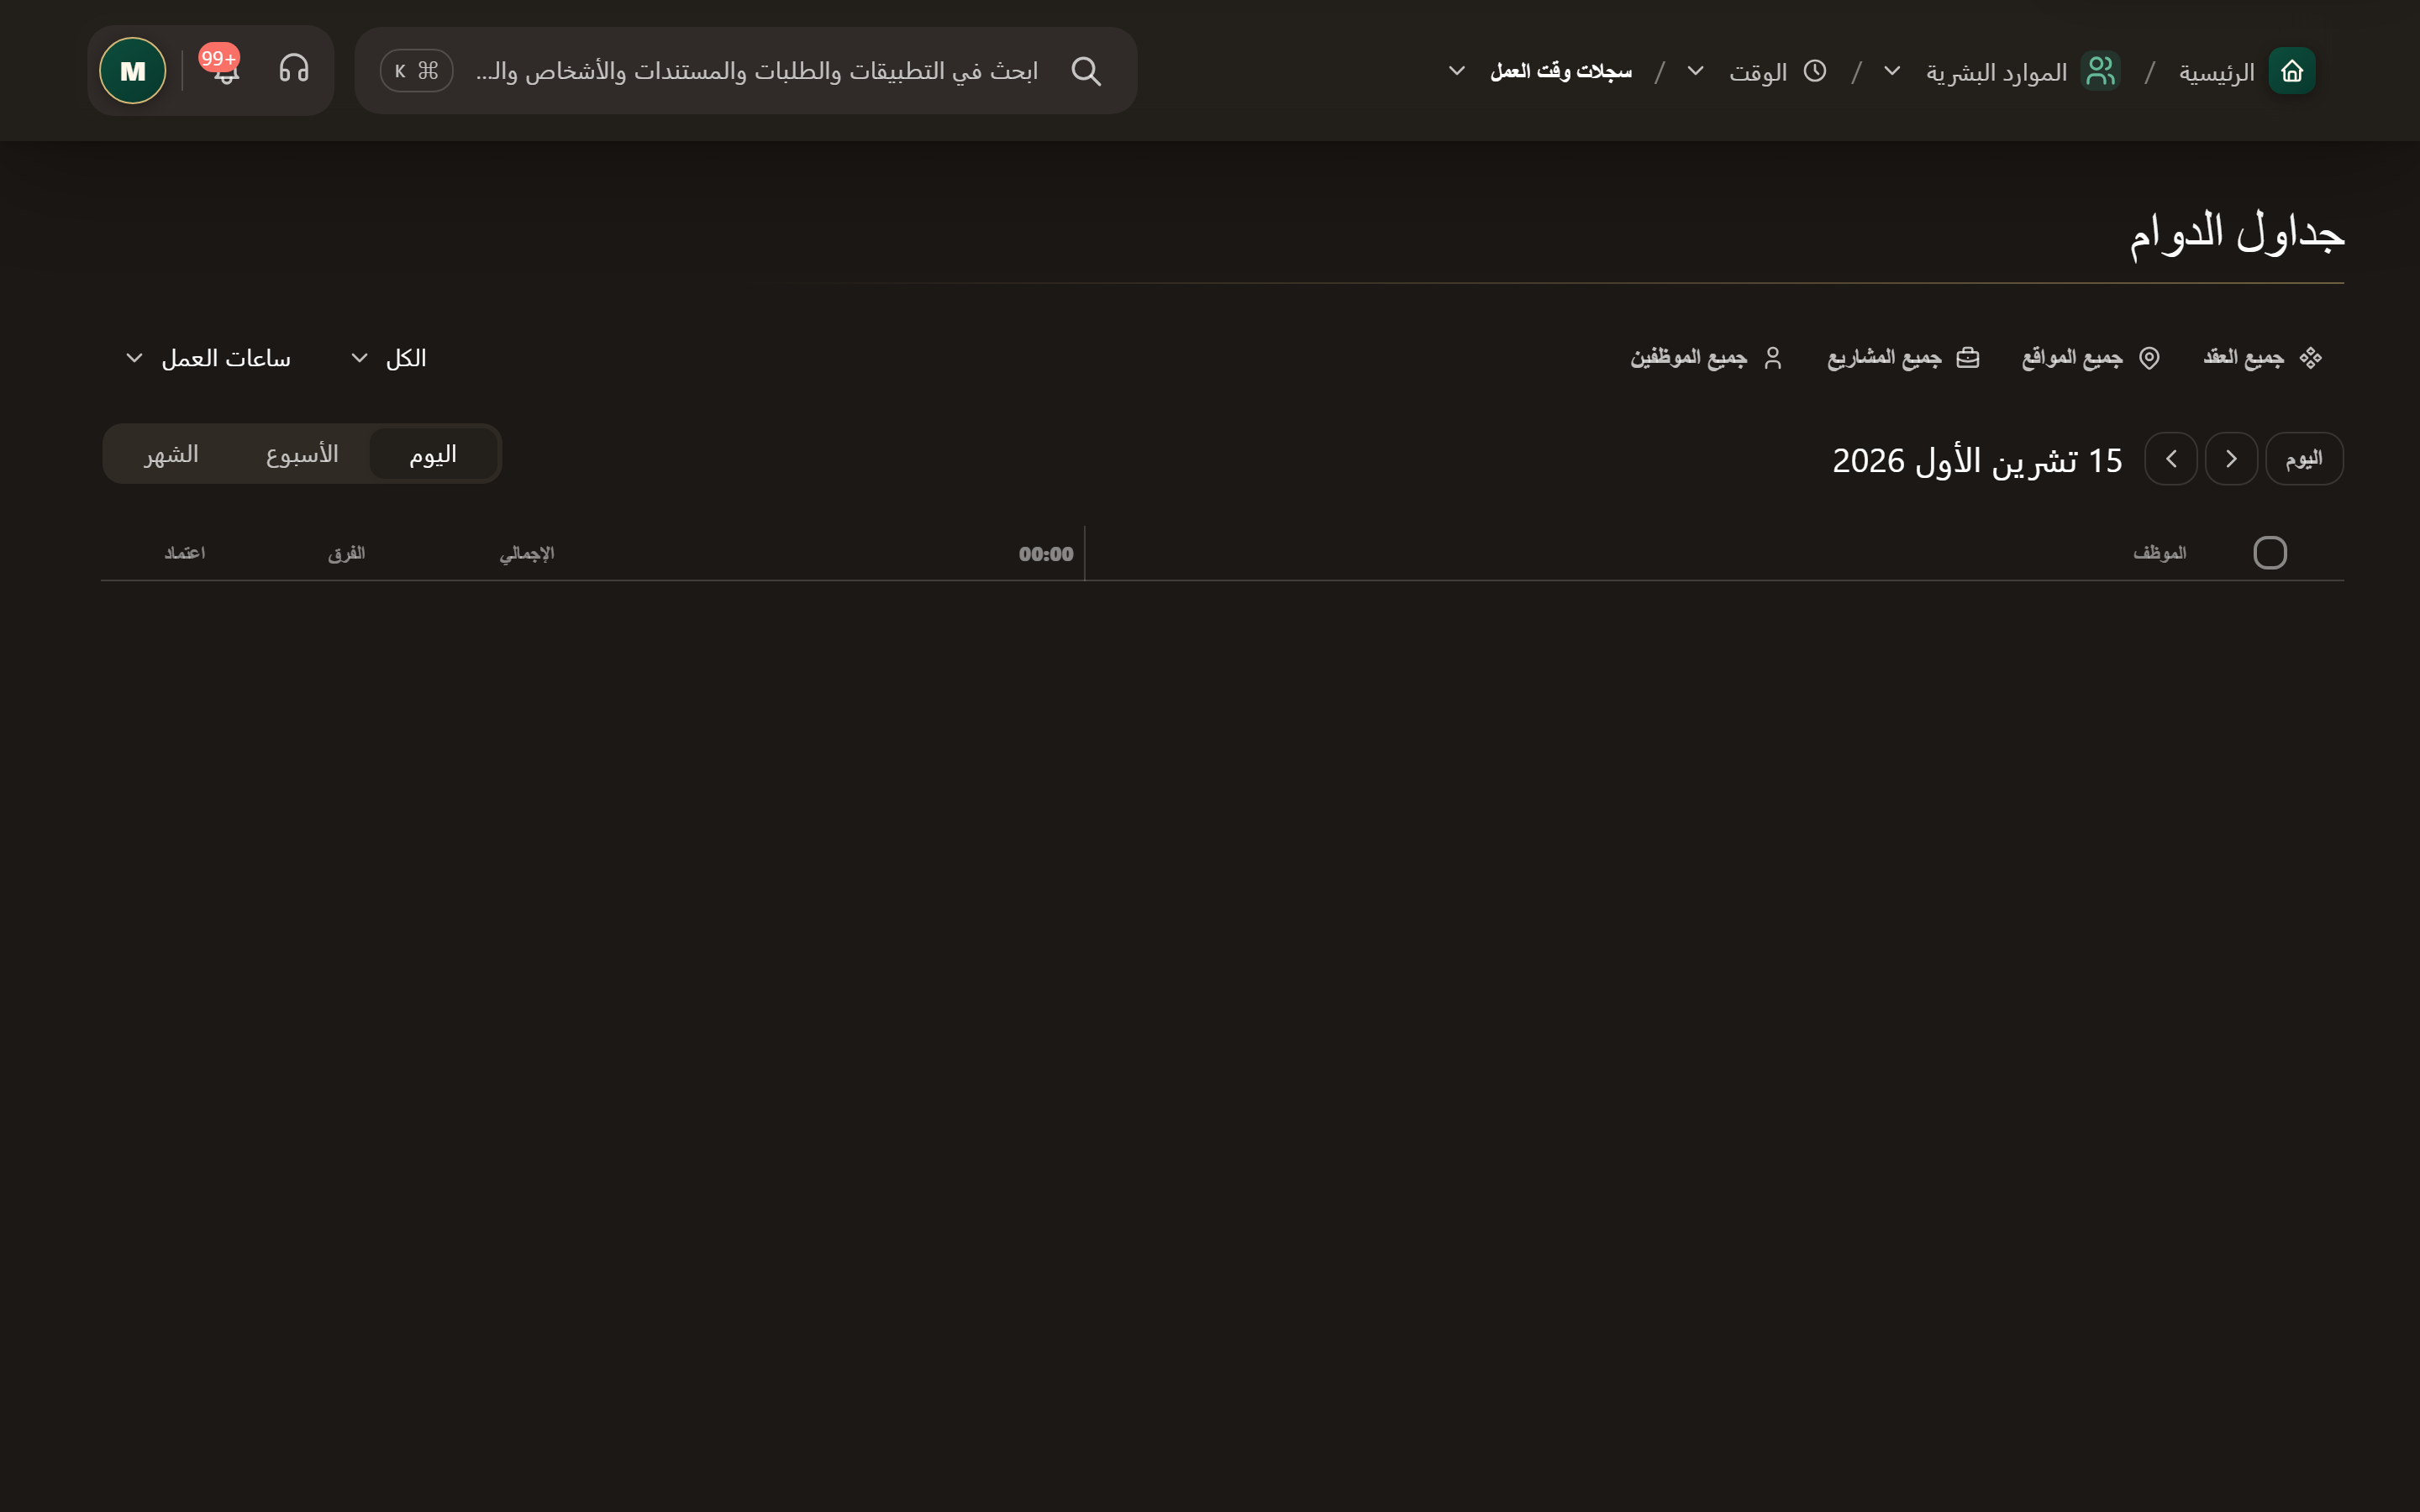
\includegraphics[width=0.95\linewidth]{figures/screens/ch03-feature-timesheets-ar.png}
\caption{جداول الدوام: الصفحة كاملة في بيئة الاختبار}
\label{fig:hr-feature-timesheets-screen}
\end{figure}

\begin{table}[H]
\centering
\caption{ما الذي تراه في جداول الدوام؟}
\label{tab:hr-feature-timesheets-data}
\rcZebra
\begin{tabularx}{\linewidth}{R{3.6cm} Y}
\rcHeaderRow
\thh{الجزء} & \thh{ماذا يعرض؟}\\
التصفية & الوحدات والمواقع والمشاريع والموظفون، والساعات: العمل فقط، أو مع الإجازات المبررة، أو مع المدفوعة.\\
الفترة & «اليوم»، أو يوم أو أسبوع أو شهر.\\
خلية اليوم & الدخول والاستراحة والخروج وإجمالي العمل؛ أو اسم العطلة.\\
الإجماليات & متوسط وقت العمل، متوسط التأخير، الإجمالي، «الفرق» عن المتوقع.\\
\end{tabularx}
\end{table}

\subsection{ما الذي يمكنك فعله؟}

\begin{itemize}
  \item عرض اليوم: خط زمني لكل موظف بالعمل والاستراحة والغياب غير المبرر.
  \item «اعتماد» صف، أو حدد عدة صفوف واعتمدها معاً؛ واعرض «الموافق فقط» أو «غير الموافق فقط».
  \item النقر على علامة الاختلاف يفتح تصحيحات الحضور. لا يمكن الإضافة أو الاستيراد هنا.
\end{itemize}

\begin{figure}[H]
\centering
\begin{tikzpicture}[node distance=0.5cm,stepBox/.append style={minimum width=6.5cm,text width=6.1cm,minimum height=0.8cm}]
  \node[stepBox] (a) {\RL{اختيار الأشخاص}\\\RL{والفترة}};
  \node[stepBox,below=of a] (b) {\RL{مراجعة الأيام}\\\RL{والإجماليات}};
  \node[stepBox,below=of b] (c) {\RL{فحص الاختلافات}};
  \draw[flowsTo] (a) -- (b);
  \draw[flowsTo] (b) -- (c);
\end{tikzpicture}
\rclegend
\caption{خطوات الاستخدام؛ الأسهم لا تعني معالجة تلقائية}
\label{fig:hr-feature-timesheets-flow}
\end{figure}

\subsection{جرّب وراجع}

\begin{enumerate}
  \item افتح «جداول الدوام»، واختر قسم الموارد البشرية و«أسبوع».
  \item اقرأ أيام كل موظف والإجماليات. إن ظهرت قيمة غير متوقعة، افتح اليوم ووردية الموظف.
  \item في عرض اليوم، اعتمد الصفوف الصحيحة.
\end{enumerate}

\textbf{تحقق:} تتغير حالة الصفوف المعتمدة. تحقق من الأشخاص والتواريخ قبل اعتبار الجدول الفارغ نقصاً في الحضور.

\clearpage
\section{أنواع الإجازات}
\label{sec:hr-feature-leave-types}

يحدد نوع الإجازة قواعدها: هل هي مدفوعة، وكيف تؤثر في الحضور، وكيف يُخصص رصيدها. مثال: «سنوية مدفوعة».

\textbf{متى تفيد؟} عرّف القاعدة مرة واحدة لتُسجَّل كل الإجازات بتصنيف موحد. النوع ليس إجازة لموظف في تاريخ محدد. \textbf{المسار:} «الموارد البشرية» / «الوقت» / «أنواع الإجازات».

\begin{figure}[H]
\centering
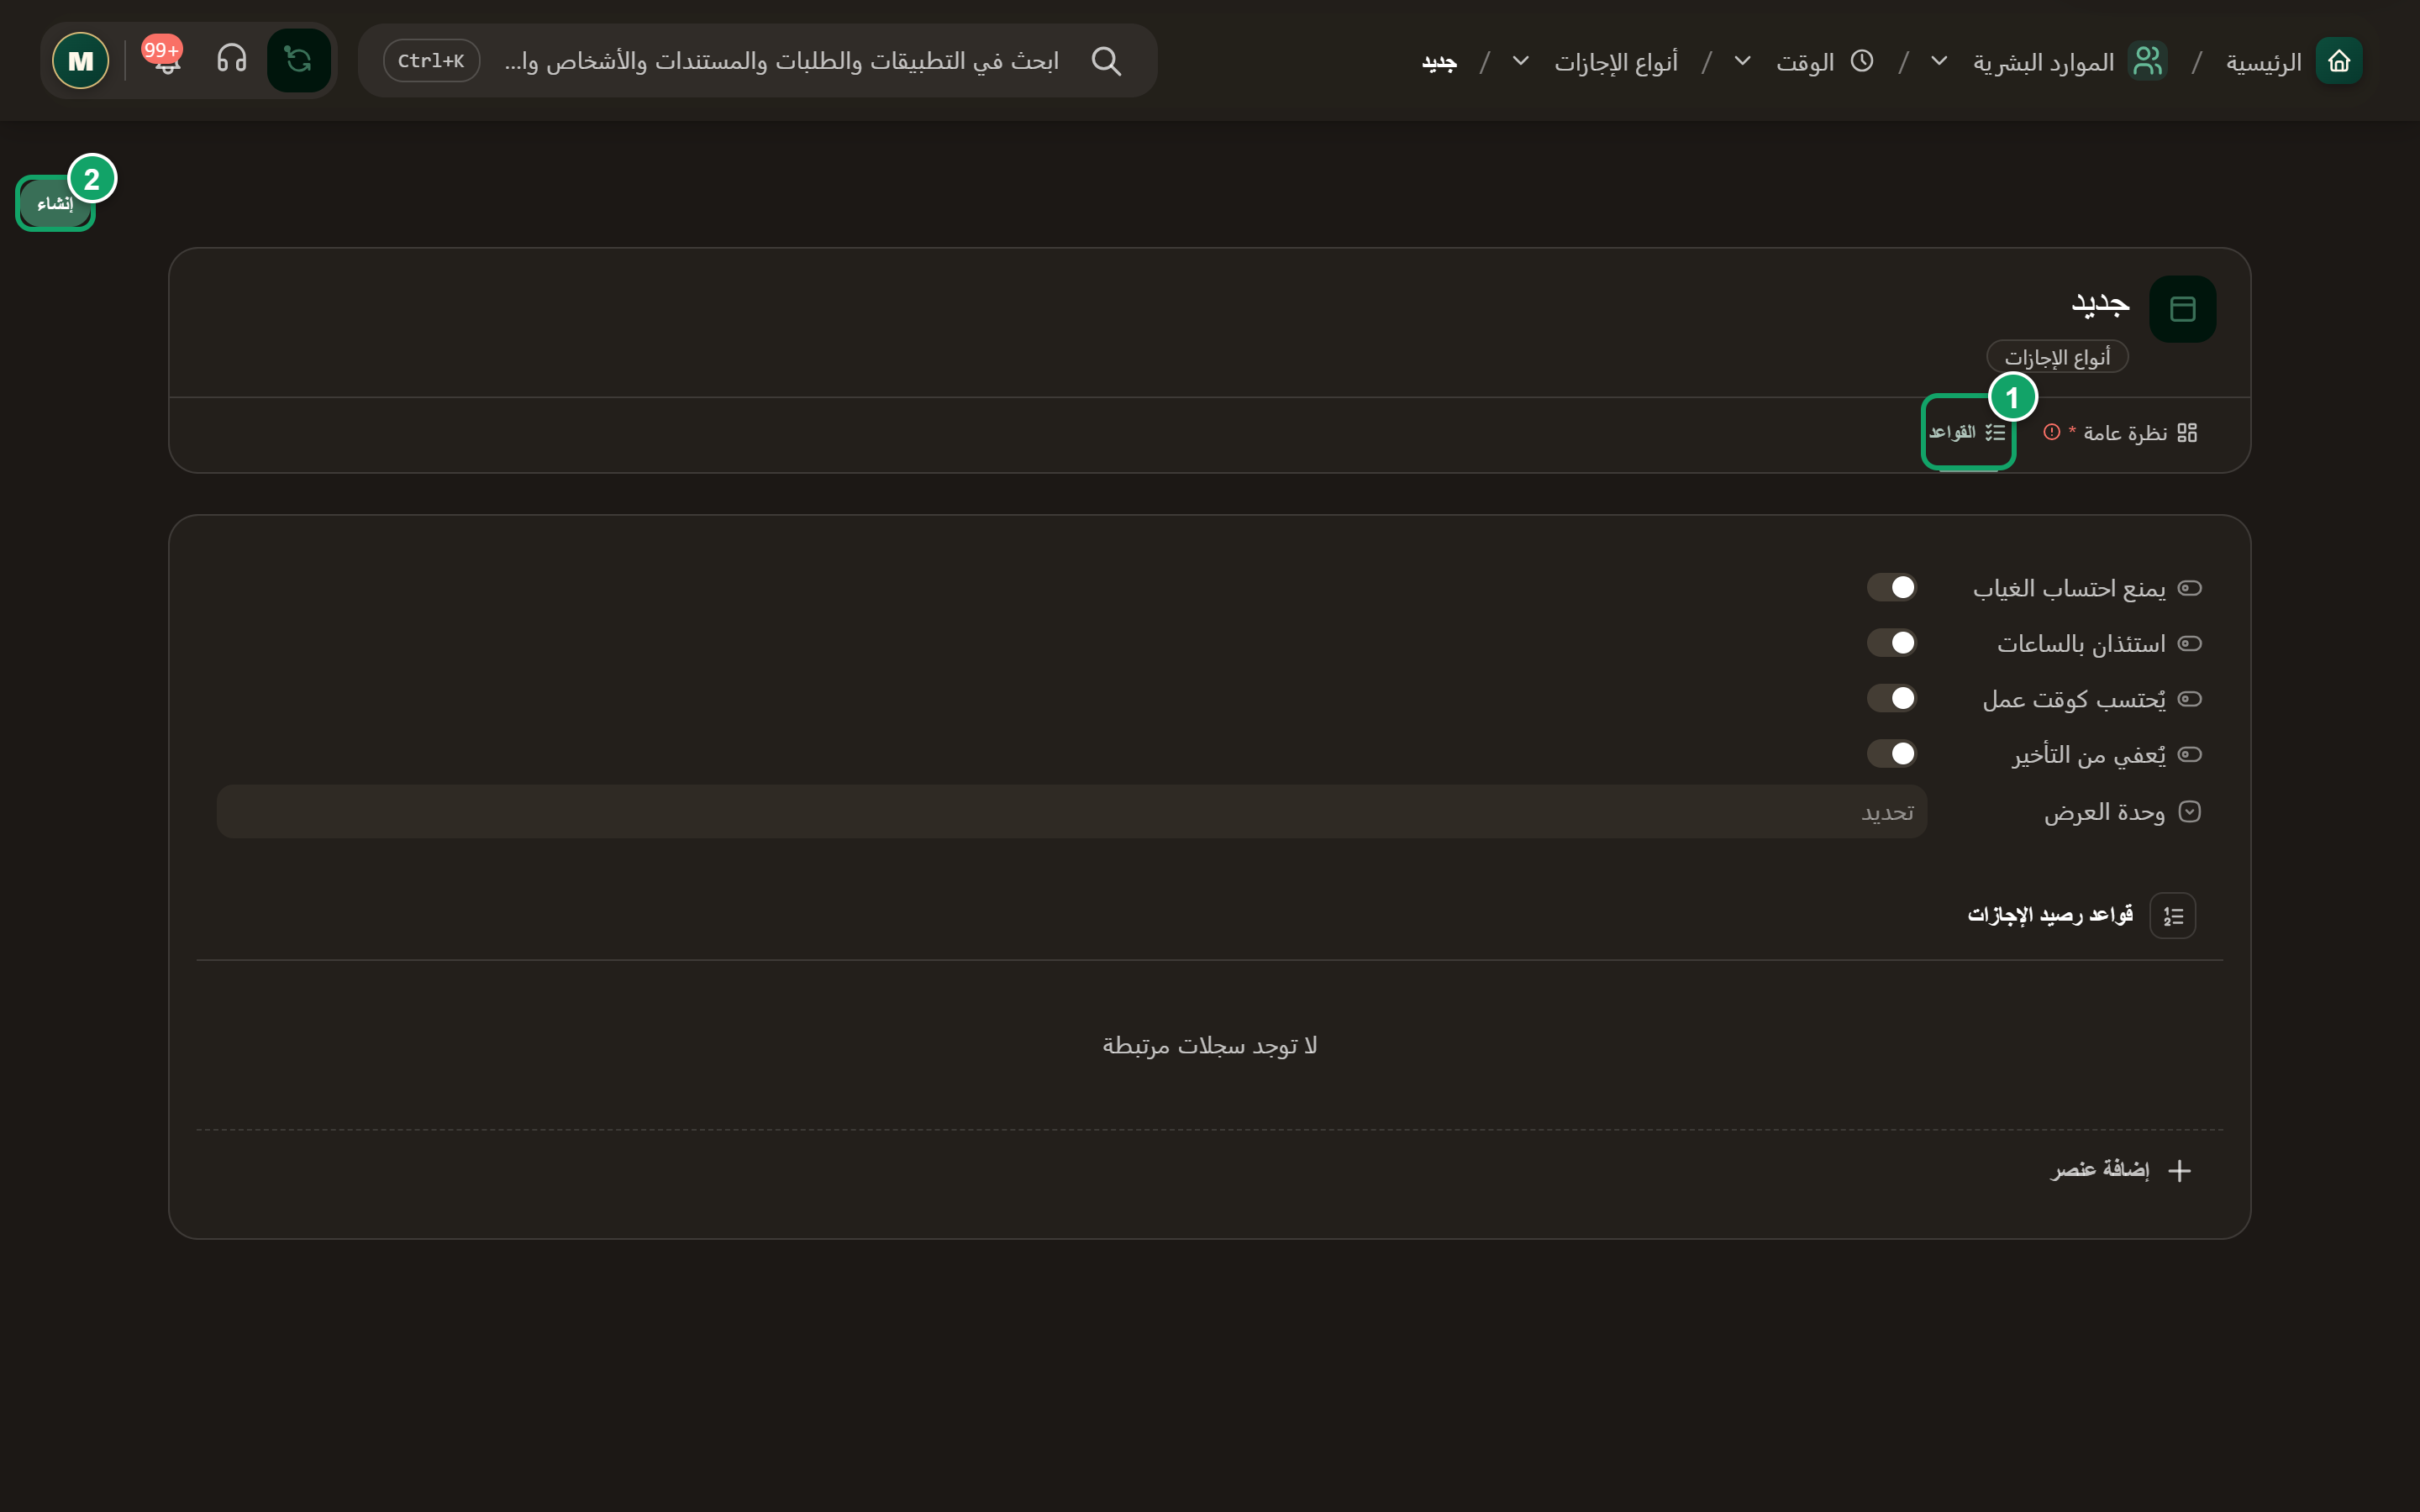
\includegraphics[width=0.95\linewidth]{figures/screens/ch03-leave-type-fields-ar.png}
\caption{أنواع الإجازات: الدفع والقواعد؛ لم يُحفظ}
\label{fig:hr-feature-leave-types-screen}
\end{figure}

\begin{table}[H]
\centering
\caption{ما الذي تسجله في نوع الإجازة؟}
\label{tab:hr-feature-leave-types-data}
\rcZebra
\begin{tabularx}{\linewidth}{R{3.6cm} Y}
\rcHeaderRow
\thh{التبويب أو الحقل} & \thh{ما الذي تضيفه؟}\\
الاسم & \req{}؛ مثل سنوية مدفوعة، مرضية، استئذان.\\
الدفع & \req{}: مدفوع، غير مدفوع، أو مدفوع جزئياً مع نسبة الدفع.\\
القواعد & يمنع احتساب الغياب، استئذان بالساعات، يُحتسب كوقت عمل، يُعفي من التأخير، وحدة العرض.\\
قواعد رصيد الإجازات & لمن يُخصص، أيام أو ساعات وكميتها، التكرار: أسبوعي أو شهري أو سنوي أو مرة واحدة، الانتهاء، تاريخ التأثير، الحالة.\\
\end{tabularx}
\end{table}

يُمنح الرصيد بقاعدة الرصيد لمن خُصصت له فقط؛ فوجود النوع لا يمنح الجميع رصيداً. لا يُحذف نوع مستخدم في إجازات.

\begin{figure}[H]
\centering
\begin{tikzpicture}[node distance=0.5cm,stepBox/.append style={minimum width=6.5cm,text width=6.1cm,minimum height=0.8cm}]
  \node[stepBox] (a) {\RL{تعريف نوع الإجازة}};
  \node[stepBox,below=of a] (b) {\RL{قاعدة الرصيد}\\\RL{والمشمولون بها}};
  \node[stepBox,below=of b] (c) {\RL{تسجيل إجازة مؤرخة}};
  \draw[flowsTo] (a) -- (b);
  \draw[flowsTo] (b) -- (c);
\end{tikzpicture}
\rclegend
\caption{خطوات الاستخدام؛ الأسهم لا تعني معالجة تلقائية}
\label{fig:hr-feature-leave-types-flow}
\end{figure}

\subsection{جرّب وراجع}

\begin{enumerate}
  \item افتح «أنواع الإجازات» وابحث عن النوع قبل إضافته.
  \item إن كنت مخوّلاً، أضف «سنوية مدفوعة» واختر «مدفوع»، ثم احفظ.
  \item في تبويب «القواعد» أضف قاعدة رصيد: المخصص لهم، «الأيام»، الكمية، «سنوي»، الانتهاء، تاريخ التأثير، «نشط». احفظ.
\end{enumerate}

\textbf{تحقق:} أعد الفتح وراجع الدفع والقاعدة. يظهر الرصيد في ملف العضو، تبويب الحضور.

\begin{figure}[H]
\centering
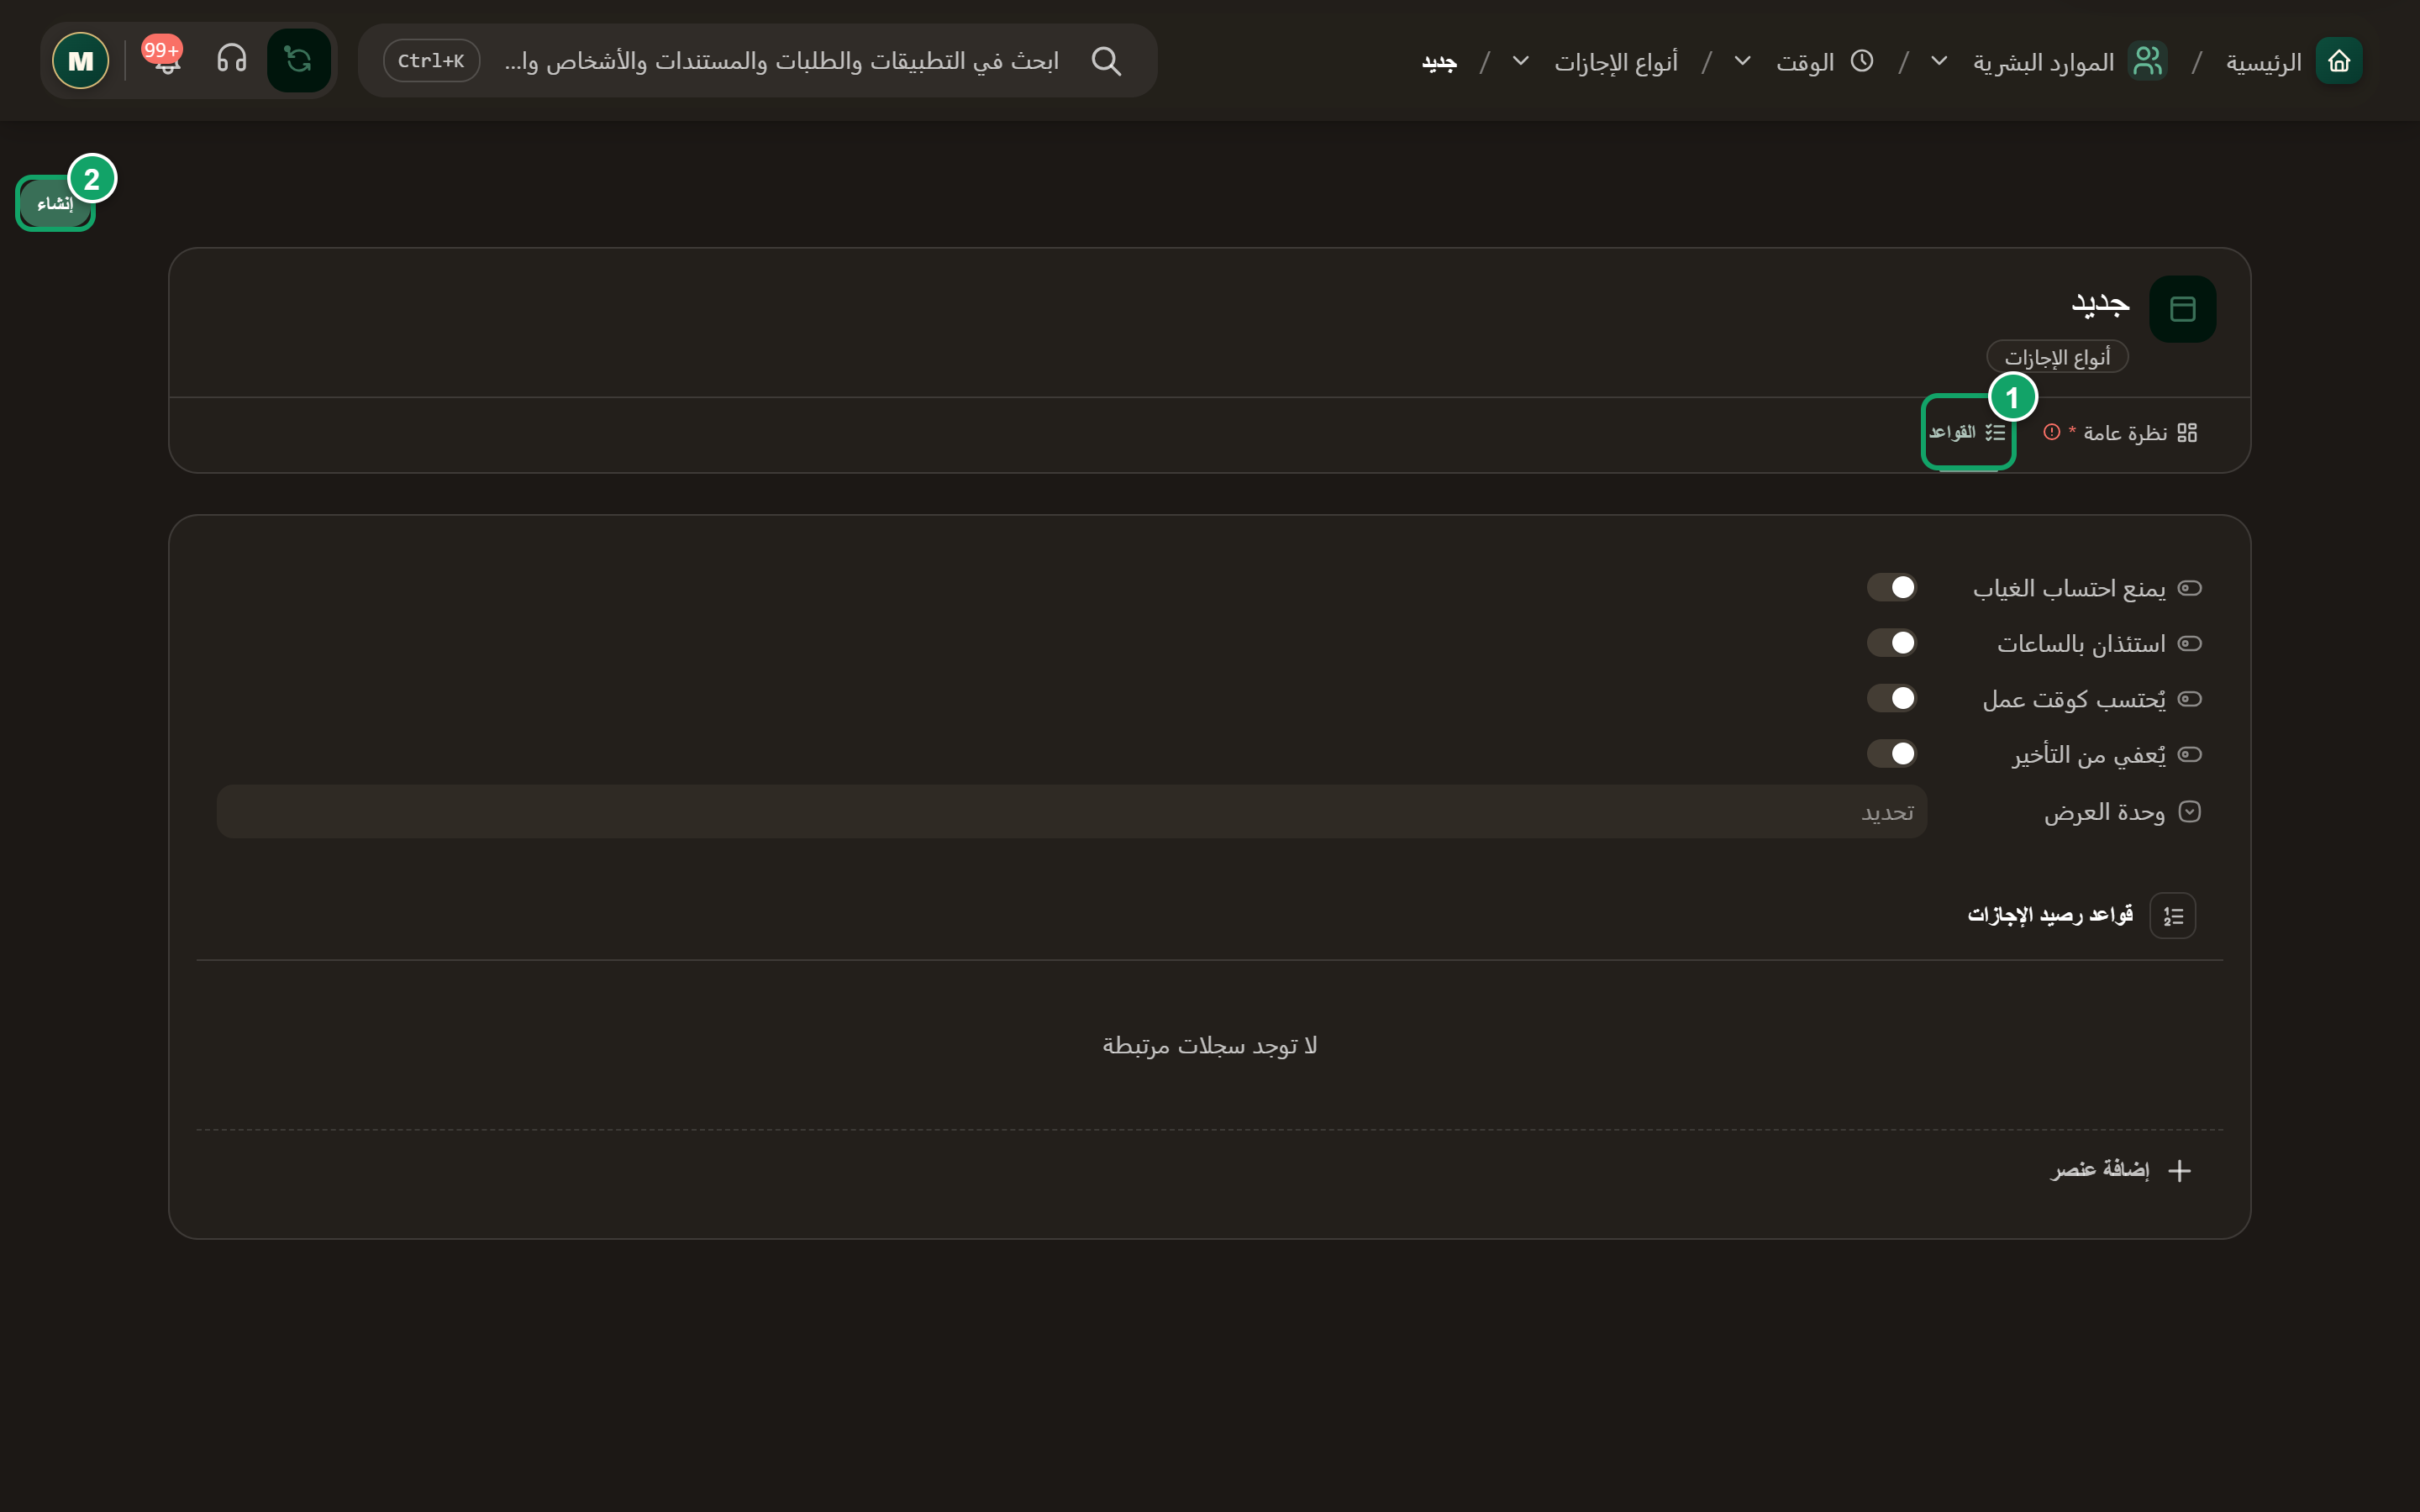
\includegraphics[width=0.95\linewidth]{figures/screens/ch03-leave-type-fields-tab1-ar.png}
\caption{تبويب «القواعد» كاملاً؛ نموذج غير محفوظ}
\label{fig:hr-leave-types-fulltab1}
\end{figure}

\clearpage
\section{الإجازات}
\label{sec:hr-feature-leaves}

يربط سجل الإجازة الموظف بنوع الإجازة، ويحدد تاريخ ووقت بدايتها ونهايتها. وله حالة: قيد الانتظار، معتمدة، أو مرفوضة.

\textbf{متى تفيد؟} تسجيل غياب سارة المعتمد ليظهر في حضورها وراتبها. العطلة مشتركة للفريق؛ الإجازة تخص موظفاً. \textbf{المسار:} «الموارد البشرية» / «الوقت» / «الإجازات».

\begin{figure}[H]
\centering
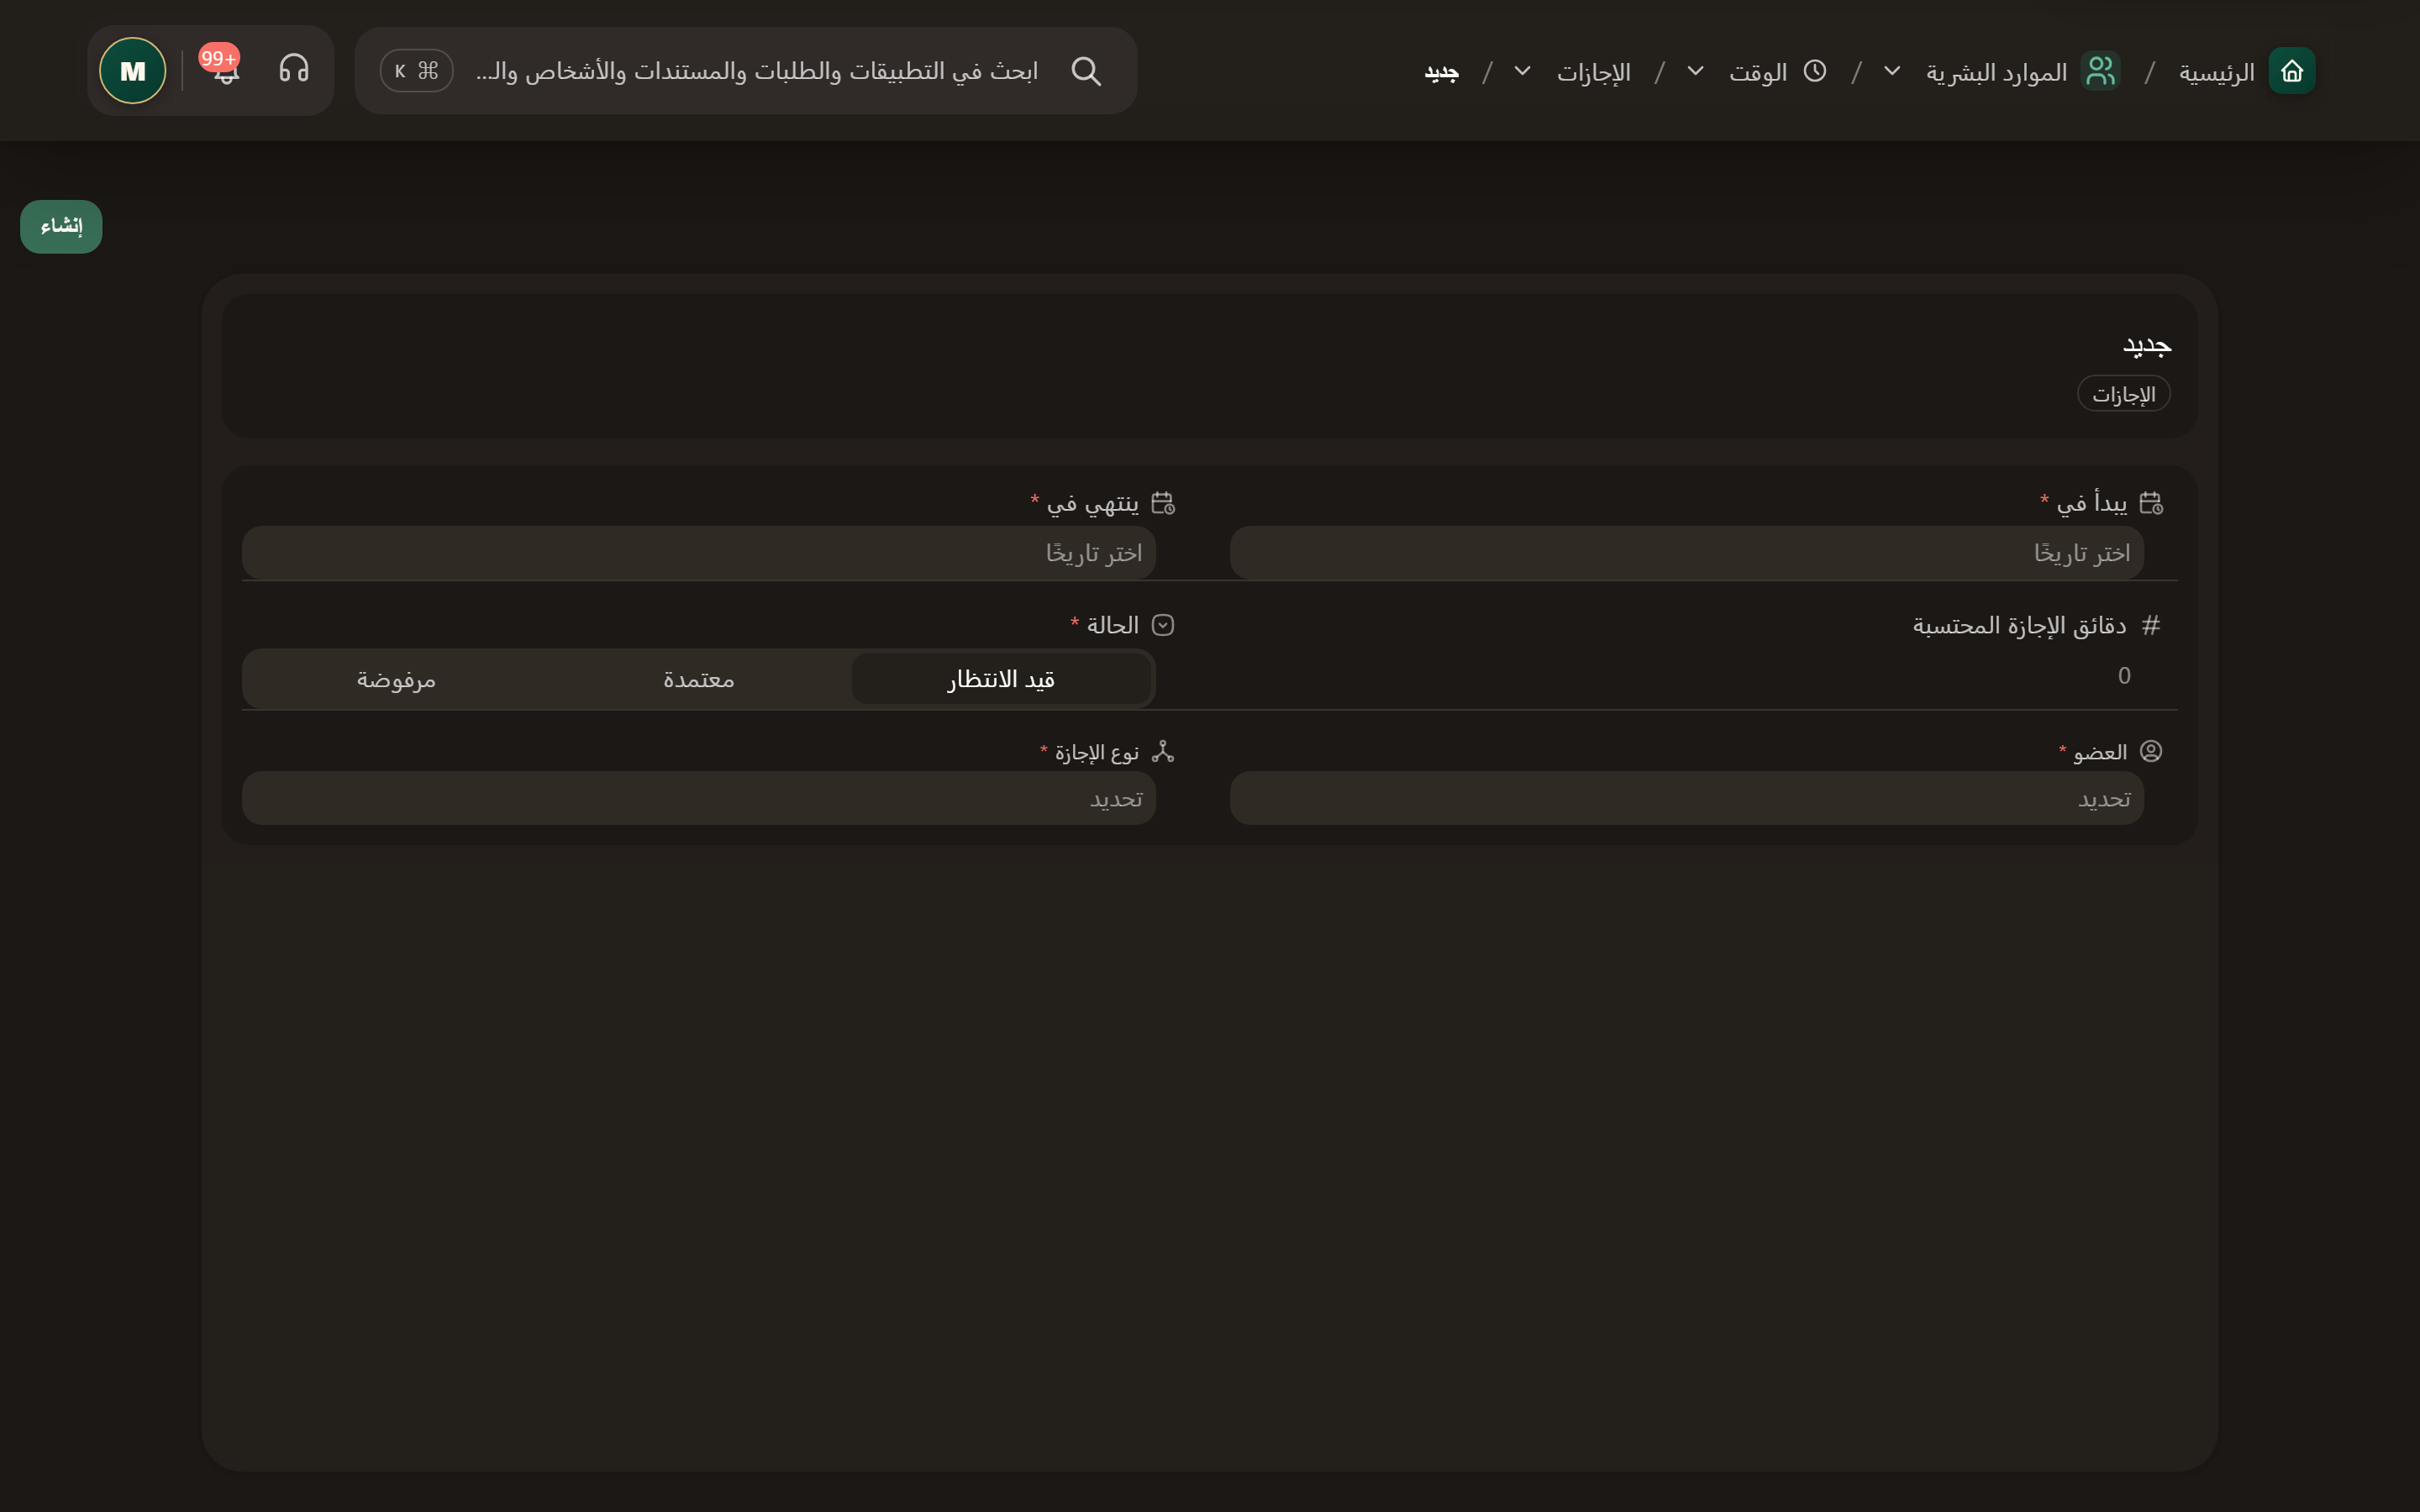
\includegraphics[width=0.95\linewidth]{figures/screens/ch03-leave-fields-ar.png}
\caption{الإجازات: الموظف والفترة والحالة؛ لم يُحفظ}
\label{fig:hr-feature-leaves-screen}
\end{figure}

\begin{table}[H]
\centering
\caption{ما الذي تسجله في الإجازة؟}
\label{tab:hr-feature-leaves-data}
\rcZebra
\begin{tabularx}{\linewidth}{R{3.6cm} Y}
\rcHeaderRow
\thh{الحقل} & \thh{ما الذي تضيفه؟}\\
العضو ونوع الإجازة & \req{}.\\
يبدأ في وينتهي في & \req{}: تاريخ ووقت.\\
الحالة & \req{}: قيد الانتظار افتراضياً، ثم معتمدة أو مرفوضة.\\
دقائق الإجازة المحتسبة & مدة الإجازة الفعلية \gen{}.\\
\end{tabularx}
\end{table}

تظهر الإجازة أيضاً في ملف العضو، تبويب الحضور. لا يوجد زر اعتماد منفصل؛ تختار الحالة في السجل نفسه بعد الموافقة.

\begin{figure}[H]
\centering
\begin{tikzpicture}[node distance=0.4cm,stepBox/.append style={minimum width=6cm,text width=5.6cm,minimum height=0.7cm}]
  \node[stepBox] (s0) {\RL{راجع النوع وطريقة}\\\RL{الدفع}};
  \node[stepBox,below=of s0] (s1) {\RL{احصل على الموافقة}};
  \node[stepBox,below=of s1] (s2) {\RL{سجّل الموظف والتاريخ}\\\RL{والمدة}};
  \node[stepBox,below=of s2] (s3) {\RL{احفظ وراجع اليوم}\\\RL{والراتب}};
  \draw[flowsTo] (s0) -- (s1);
  \draw[flowsTo] (s1) -- (s2);
  \draw[flowsTo] (s2) -- (s3);
\end{tikzpicture}
\rclegend
\caption{من نوع الإجازة إلى مراجعة يوم الموظف}
\label{fig:hr-leave-flow}
\end{figure}

\subsection{جرّب وراجع}

\begin{enumerate}
  \item تأكد من الموافقة والتواريخ ورصيد سارة. افتح «الإجازات» وابحث عن سجل سابق.
  \item أضف: سارة، «سنوية مدفوعة»، تاريخ ووقت البدء والانتهاء، والحالة «معتمدة». احفظ.
  \item أعد فتح السجل وراجع المدة المحتسبة، ثم افتح اليوم في حضوري.
\end{enumerate}

\textbf{تحقق:} يظهر اليوم في حضوري مبرراً بإجازة. إن غاب الأثر، راجع التاريخ والنوع والحالة؛ «قيد الانتظار» لا تبرر الغياب.

\clearpage
\section{مجموعات العطل الرسمية}
\label{sec:hr-feature-holiday-groups}

مجموعة العطل تقويم مشترك للعطل الرسمية، ويتبعه من تُسند إليهم المجموعة.

\textbf{متى تفيد؟} يتبع الفريق تقويم عطل واحداً، دون تسجيل كل عطلة إجازةً لكل موظف. \textbf{المسار:} «الموارد البشرية» / «الوقت» / «مجموعات العطل الرسمية».

\begin{figure}[H]
\centering
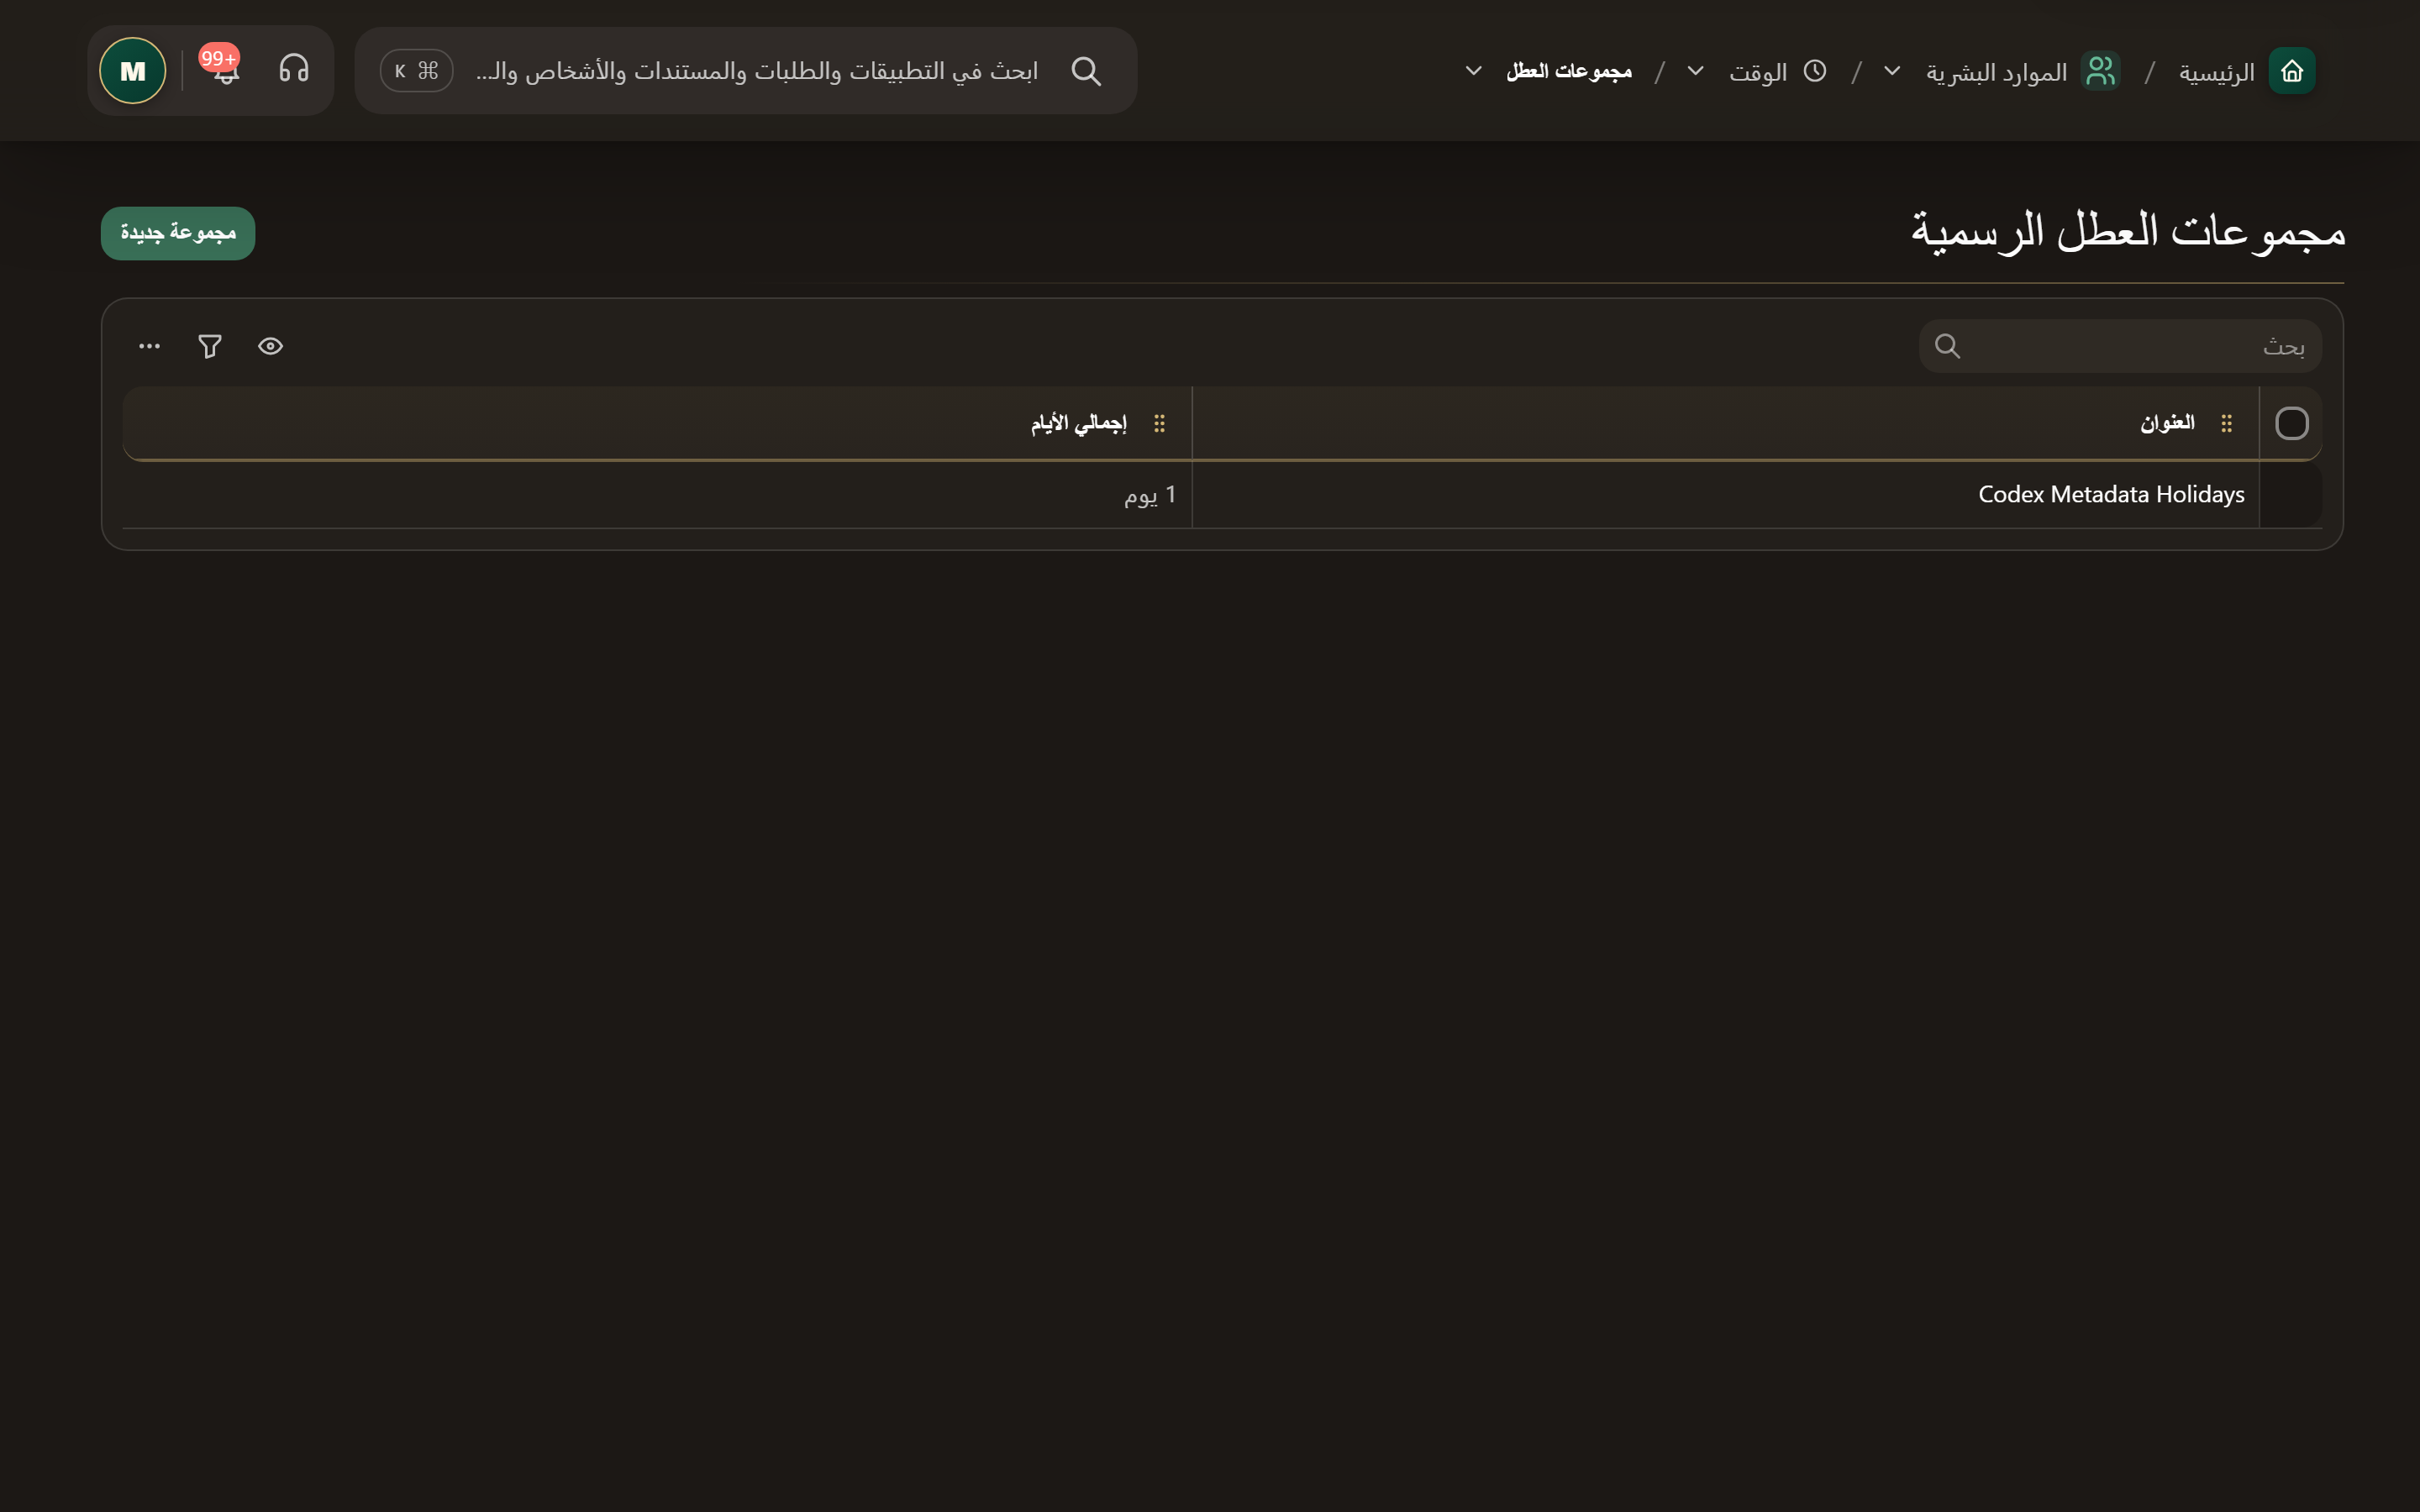
\includegraphics[width=0.95\linewidth]{figures/screens/ch03-feature-holiday-groups-ar.png}
\caption{مجموعات العطل الرسمية: الصفحة كاملة في بيئة الاختبار}
\label{fig:hr-feature-holiday-groups-screen}
\end{figure}

\begin{table}[H]
\centering
\caption{ما الذي تسجله في مجموعة العطل؟}
\label{tab:hr-feature-holiday-groups-data}
\rcZebra
\begin{tabularx}{\linewidth}{R{3.6cm} Y}
\rcHeaderRow
\thh{التبويب أو الحقل} & \thh{ما الذي تضيفه؟}\\
المجموعة & اسم المجموعة \req{}؛ عدد العطل وإجمالي الأيام \gen{}.\\
العطل & الاسم \req{}، ثم يوم كامل بتاريخه، أو يوم جزئي بساعاته، أو نطاق من تاريخ إلى تاريخ.\\
المُكلف & من يتبع المجموعة: أعضاء أو أقسام أو المؤسسة كلها.\\
\end{tabularx}
\end{table}

\begin{itemize}
  \item «مجموعة جديدة»، و«إضافة عطلة»، والبحث في العطل وتعديلها أو حذفها.
  \item لا يمكن إضافة عطلتين في التاريخ نفسه. ويمكن تحديد مجموعة عطل مختلفة في تعيين الموظف.
\end{itemize}

\begin{figure}[H]
\centering
\begin{tikzpicture}[node distance=0.5cm,stepBox/.append style={minimum width=6.5cm,text width=6.1cm,minimum height=0.8cm}]
  \node[stepBox] (a) {\RL{تجهيز التقويم المشترك}};
  \node[stepBox,below=of a] (b) {\RL{إضافة تواريخ العطل}};
  \node[stepBox,below=of b] (c) {\RL{مراجعة المُكلفين}};
  \draw[flowsTo] (a) -- (b);
  \draw[flowsTo] (b) -- (c);
\end{tikzpicture}
\rclegend
\caption{خطوات الاستخدام؛ الأسهم لا تعني معالجة تلقائية}
\label{fig:hr-feature-holiday-groups-flow}
\end{figure}

\subsection{جرّب وراجع}

\begin{enumerate}
  \item افتح «مجموعات العطل الرسمية»، ثم المجموعة المناسبة أو «مجموعة جديدة».
  \item «إضافة عطلة»: الاسم والتاريخ، واختر يوماً كاملاً أو جزئياً أو نطاقاً، ثم احفظ.
  \item في «المُكلف» اختر قسم الموارد البشرية أو المؤسسة كلها، واحفظ.
\end{enumerate}

\textbf{تحقق:} يظهر يوم العطلة بحالة «عطلة» في حضوري لكل موظف مشمول.

\clearpage
\section{تصحيحات الحضور}
\label{sec:hr-feature-attendance-corrections}

تجمع هذه الصفحة الأيام التي تحتاج تصحيحاً، مثل بصمة ناقصة، لتصحح بصماتها وتوافق على الطلب أو ترفضه.

\textbf{متى تفيد؟} لمعالجة أيام الفريق الخاطئة قبل الرواتب، بدلاً من البحث عنها يوماً بعد يوم. \textbf{المسار:} «الموارد البشرية» / «الوقت» / «تصحيحات الحضور».

\begin{figure}[H]
\centering
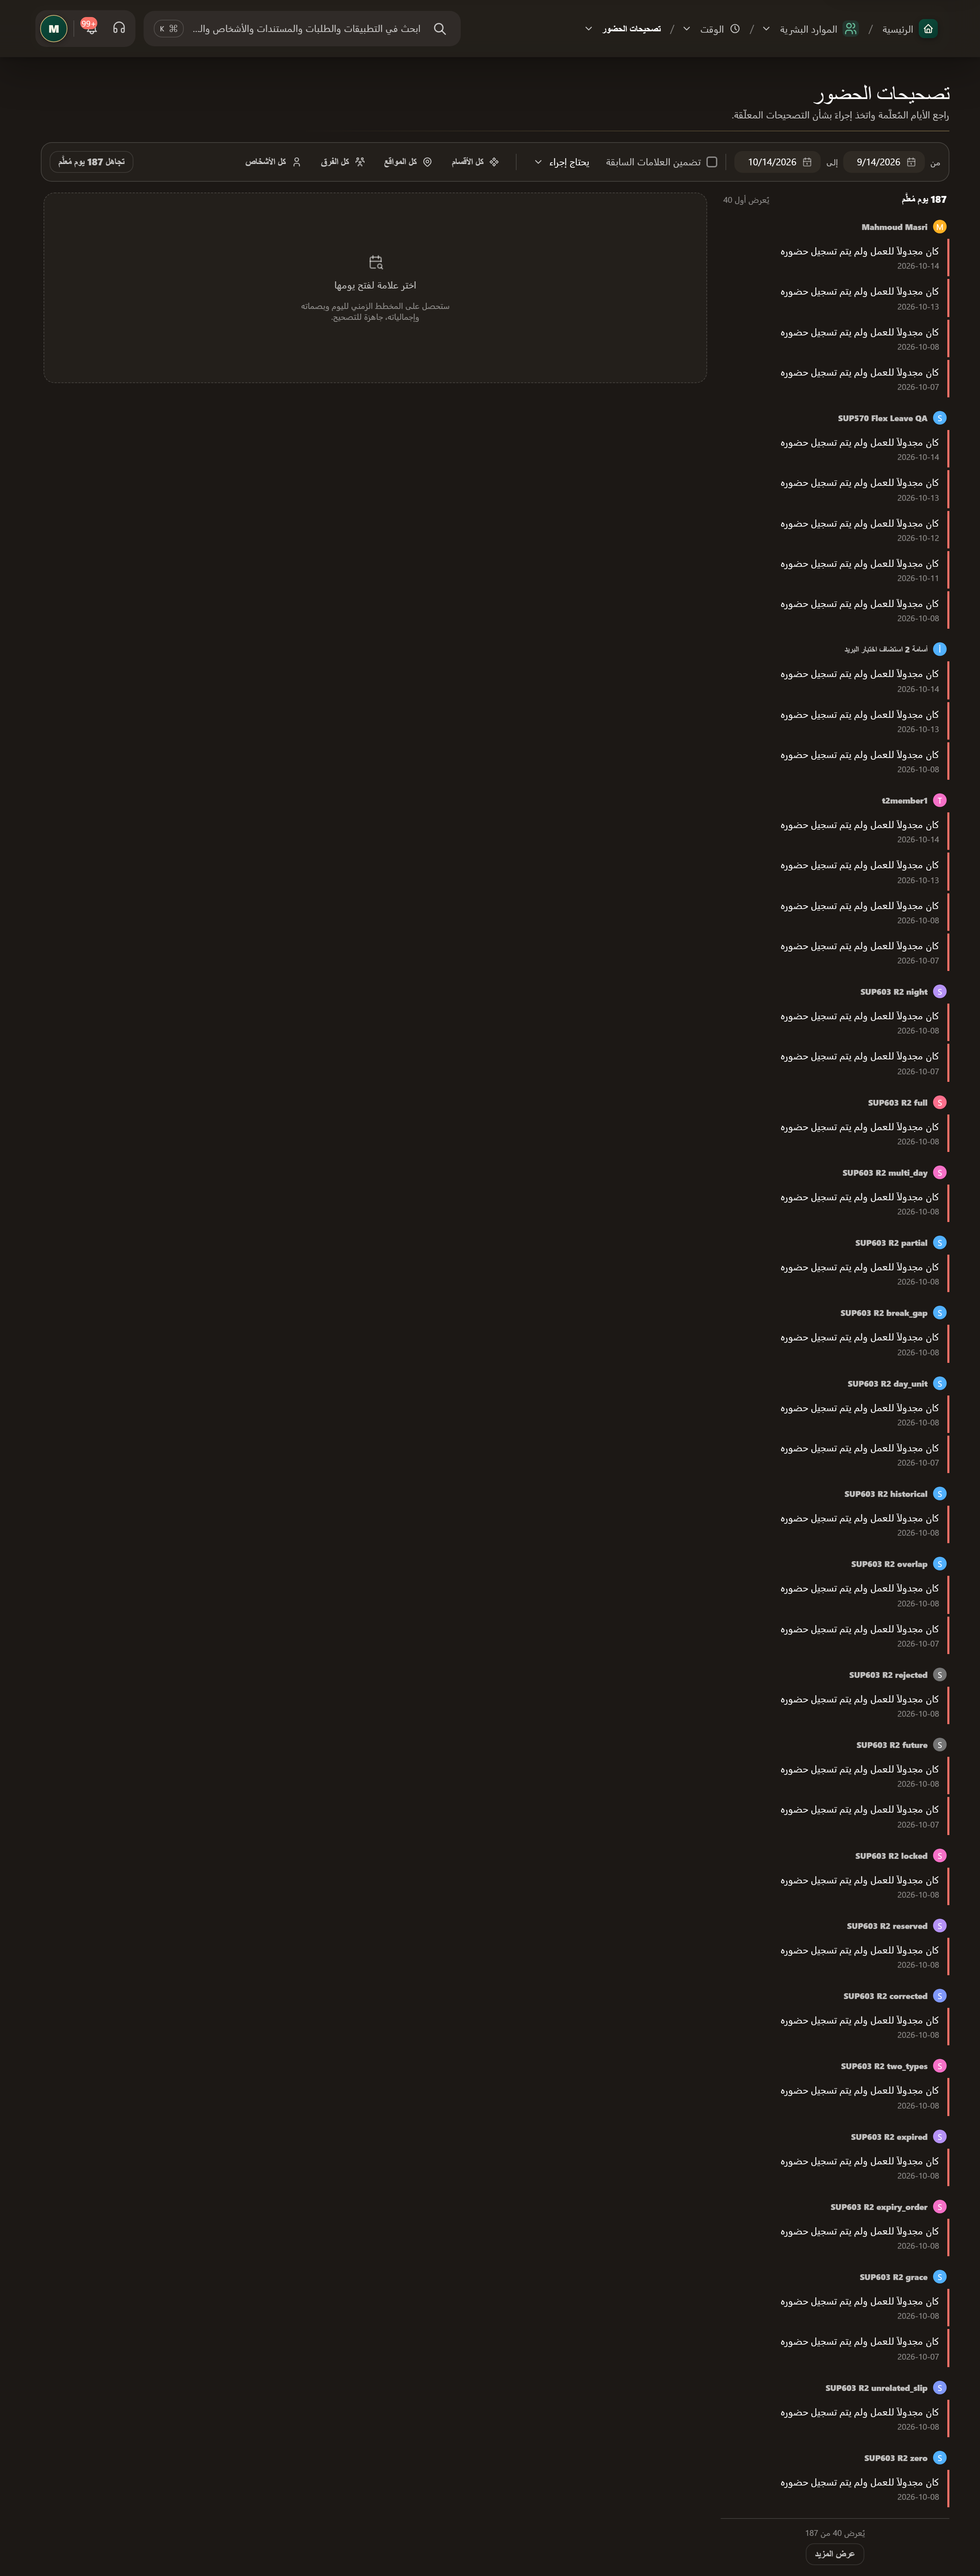
\includegraphics[width=0.95\linewidth]{figures/screens/ch03-feature-attendance-corrections-ar.png}
\caption{تصحيحات الحضور: الصفحة كاملة في بيئة الاختبار}
\label{fig:hr-feature-attendance-corrections-screen}
\end{figure}

\begin{table}[H]
\centering
\caption{ما الذي تراه في تصحيحات الحضور؟}
\label{tab:hr-feature-attendance-corrections-data}
\rcZebra
\begin{tabularx}{\linewidth}{R{3.6cm} Y}
\rcHeaderRow
\thh{الجزء} & \thh{ماذا يعرض؟}\\
التصفية & من وإلى؛ يحتاج إجراء، بانتظار الاعتماد، تمت المعالجة، الكل؛ الأقسام والمواقع والفرق والأشخاص.\\
سبب العلامة & لا انصراف، لا حضور، دخول مكرر، مدة غير منطقية، بصمة خارج الوردية، غياب في يوم مجدول.\\
لوحة اليوم & البصمات ومصدرها: جهاز أو إدخال يدوي؛ الخط الزمني؛ العمل والاستراحة مقابل الوردية.\\
الطلب & السبب والتبرير، ومن طلبه، والتغييرات، وآخر موعد للاعتماد.\\
\end{tabularx}
\end{table}

\subsection{ما الذي يمكنك فعله؟}

\begin{itemize}
  \item أضف بصمة، أو غيّر وقتها أو اتجاهها، أو احذفها. ليوم بلا بصمات: «تسجيل إجازة».
  \item «حفظ التصحيح»، «إرسال للموافقة»، «موافقة»، «رفض»؛ حسب دورك.
  \item تجاهل علامة: «تأكيد الغياب» أو «ليست مشكلة». لتجاهل عدة أيام معاً، اكتب عددها للتأكيد.
  \item مهلة التصحيح تُضبط أسفل صفحة سياسة الحضور.
\end{itemize}

\begin{figure}[H]
\centering
\begin{tikzpicture}[node distance=0.5cm,stepBox/.append style={minimum width=6.5cm,text width=6.1cm,minimum height=0.8cm}]
  \node[stepBox] (a) {\RL{مراجعة اليوم}};
  \node[stepBox,below=of a] (b) {\RL{إرسال التصحيح}};
  \node[stepBox,below=of b] (c) {\RL{مراجعة القرار واليوم}};
  \draw[flowsTo] (a) -- (b);
  \draw[flowsTo] (b) -- (c);
\end{tikzpicture}
\rclegend
\caption{خطوات الاستخدام؛ الأسهم لا تعني معالجة تلقائية}
\label{fig:hr-feature-attendance-corrections-flow}
\end{figure}

\subsection{جرّب وراجع}

\begin{enumerate}
  \item افتح «تصحيحات الحضور»، واختر «يحتاج إجراء» وقسم الموارد البشرية.
  \item افتح اليوم، وأضف البصمة الناقصة، واختر السبب، ثم «إرسال للموافقة».
\end{enumerate}

\textbf{تحقق:} ينتقل اليوم إلى «بانتظار الاعتماد»، ثم «تمت المعالجة» بعد القرار. إن لم يتوفر الإجراء، راجع المهلة والصلاحيات.

\clearpage
\section{سياسة الحضور}
\label{sec:hr-feature-attendance-policy}

تحدد سياسة الحضور كيفية تقييم الوقت المسجل: متى يُعفى الموظف من التأخر، ومتى يُحتسب الوقت عملاً إضافياً، وعلى من تنطبق القواعد.

\textbf{متى تفيد؟} مراجعة موحدة للحضور. الوردية تحدد الوقت المتوقع، والسياسة تقيّم الفرق. \textbf{المسار:} «الموارد البشرية» / «الوقت» / «سياسة الحضور».

\begin{figure}[H]
\centering
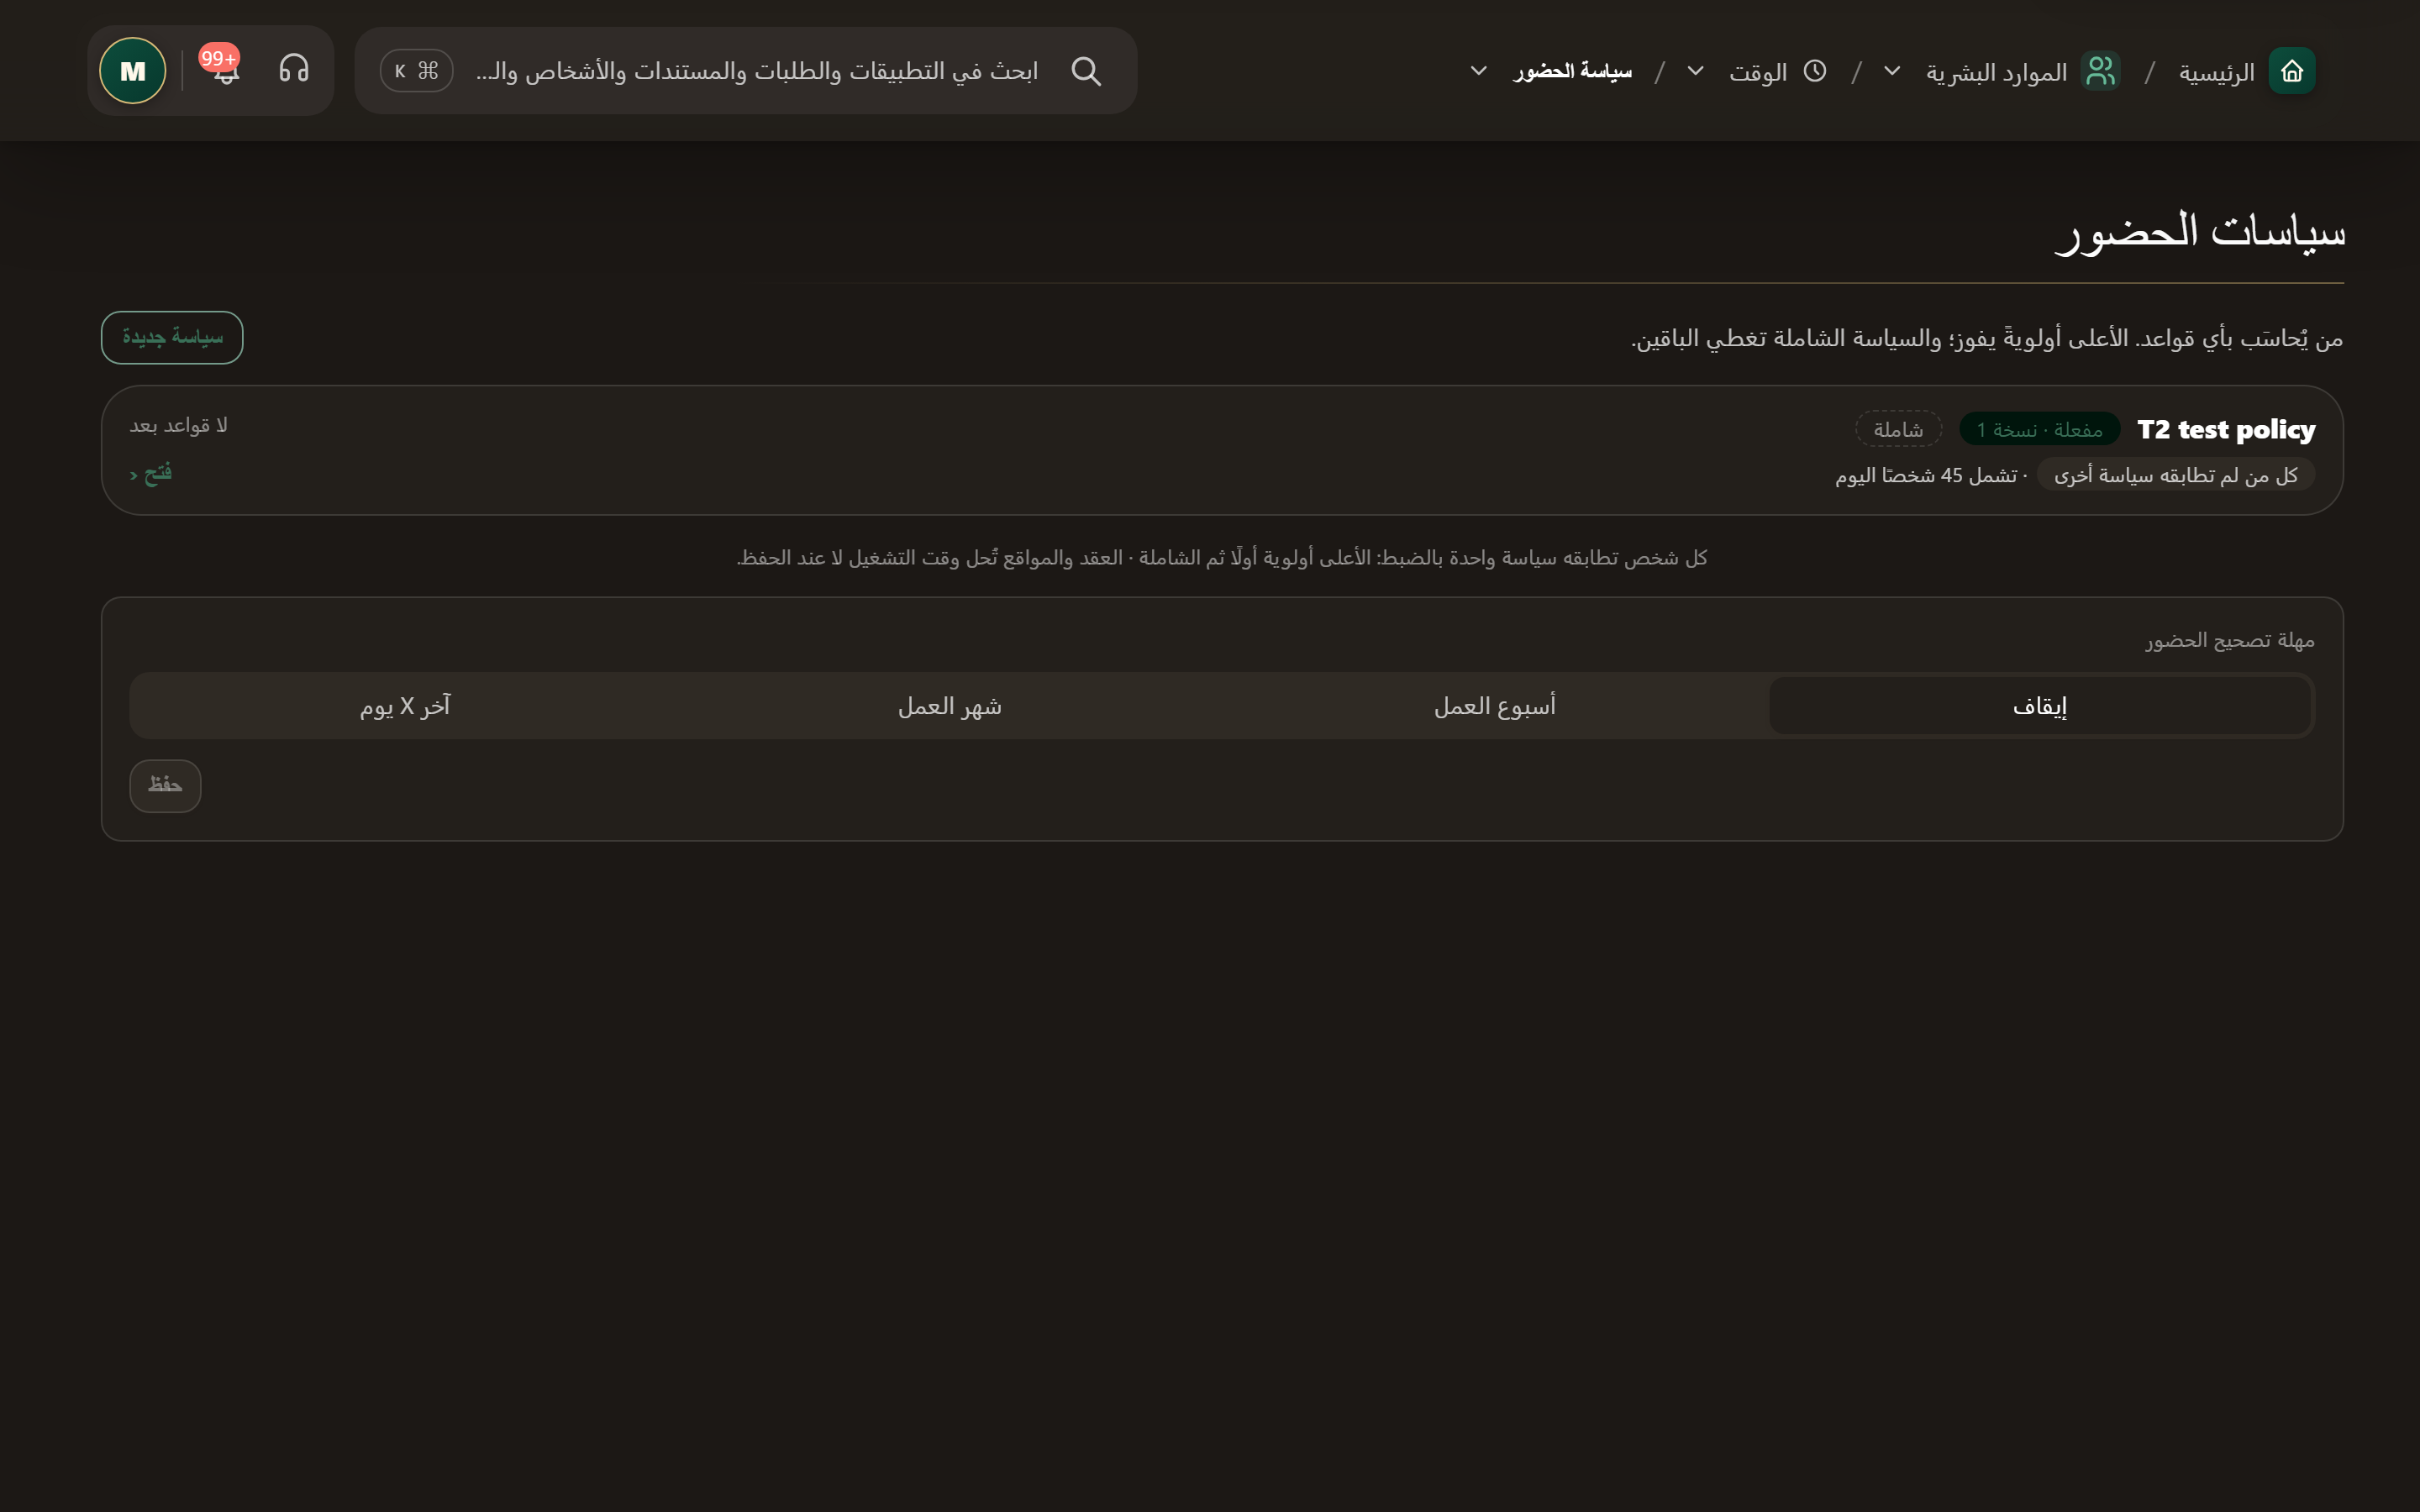
\includegraphics[width=0.95\linewidth]{figures/screens/ch03-feature-attendance-policy-ar.png}
\caption{سياسة الحضور: الصفحة كاملة في بيئة الاختبار}
\label{fig:hr-feature-attendance-policy-screen}
\end{figure}

\begin{table}[H]
\centering
\caption{ما الذي تضبطه في السياسة؟}
\label{tab:hr-feature-attendance-policy-data}
\rcZebra
\begin{tabularx}{\linewidth}{R{3.6cm} Y}
\rcHeaderRow
\thh{التبويب أو الجزء} & \thh{ما الذي تضبطه؟}\\
المسند إليهم & أشخاص أو أقسام أو مواقع أو مناصب أو مجموعات. تغطي السياسة الشاملة كل من لا تشمله سياسة أخرى.\\
قواعد بالدقائق & التأخر، المغادرة المبكرة، تجاوز الاستراحة، نقص الساعات، العمل الإضافي.\\
قواعد اليوم الكامل & الغياب، العمل في يوم الراحة، العمل في العطلة.\\
النطاقات & لكل نطاق من الدقائق (مثل \en{0–10}): يُعفى منه أو يُحتسب بمضاعف، ويُسجَّل بتصنيف مثل «تأخير مسموح».\\
الحالة & مسودة، مفعلة بإصدار، معطلة؛ وعند التعارض تُطبق السياسة الأعلى أولوية.\\
\end{tabularx}
\end{table}

\subsection{ما الذي يمكنك فعله؟}

\begin{itemize}
  \item «إنشاء سياسة»: تبدأ السياسة مسودةً، ثم «تعديل القواعد» و«حفظ المسودة» و«تفعيل».
  \item «جرّب وقتاً» للتأخر: اختر وردية ووقت وصول وشاهد النتيجة.
  \item «محاكاة»: «إعادة احتساب الشهر الماضي» بالمسودة قبل تفعيلها.
  \item «تعطيل السياسة»، و«حذف السياسة» إن لم تُفعّل قط.
\end{itemize}

\begin{figure}[H]
\centering
\begin{tikzpicture}[node distance=0.5cm,stepBox/.append style={minimum width=6.5cm,text width=6.1cm,minimum height=0.8cm}]
  \node[stepBox] (a) {\RL{اختيار المشمولين بالسياسة}};
  \node[stepBox,below=of a] (b) {\RL{مراجعة قواعد الحضور}};
  \node[stepBox,below=of b] (c) {\RL{فحص نتيجة تجريبية}};
  \draw[flowsTo] (a) -- (b);
  \draw[flowsTo] (b) -- (c);
\end{tikzpicture}
\rclegend
\caption{خطوات الاستخدام؛ الأسهم لا تعني معالجة تلقائية}
\label{fig:hr-feature-attendance-policy-flow}
\end{figure}

\subsection{جرّب وراجع}

\begin{enumerate}
  \item يفتح المسؤول المخوّل «سياسة الحضور» ويختار السياسة، ثم «تعديل القواعد».
  \item في التأخر أضف نطاقاً: من \en{0} إلى \en{10} دقائق يُعفى منه. احفظ المسودة.
  \item استخدم «جرّب وقتاً» و«محاكاة»، ثم «تفعيل» عند صحة النتيجة.
\end{enumerate}

\textbf{تحقق:} راجع يوماً فعلياً في حضوري بعد التفعيل. علامة تنبيه وحدها لا تعني خصماً من الراتب.

\clearpage
\section{أجهزة الحضور}
\label{sec:hr-feature-attendance-terminals}

تربط هذه الصفحة أجهزة البصمة بالنظام. لكل موقع شبكة يعمل فيها برنامج اتصال يسمى «وكيل الحضور»، ويرسل البصمات تلقائياً، ثم تُطابق البصمات مع الأعضاء.

\textbf{متى تفيد؟} عندما يأتي الحضور من جهاز فعلي. وجود الجهاز في القائمة لا يثبت وصول بصماته. \textbf{المسار:} «الموارد البشرية» / «الوقت» / «أجهزة الحضور».

\begin{figure}[H]
\centering
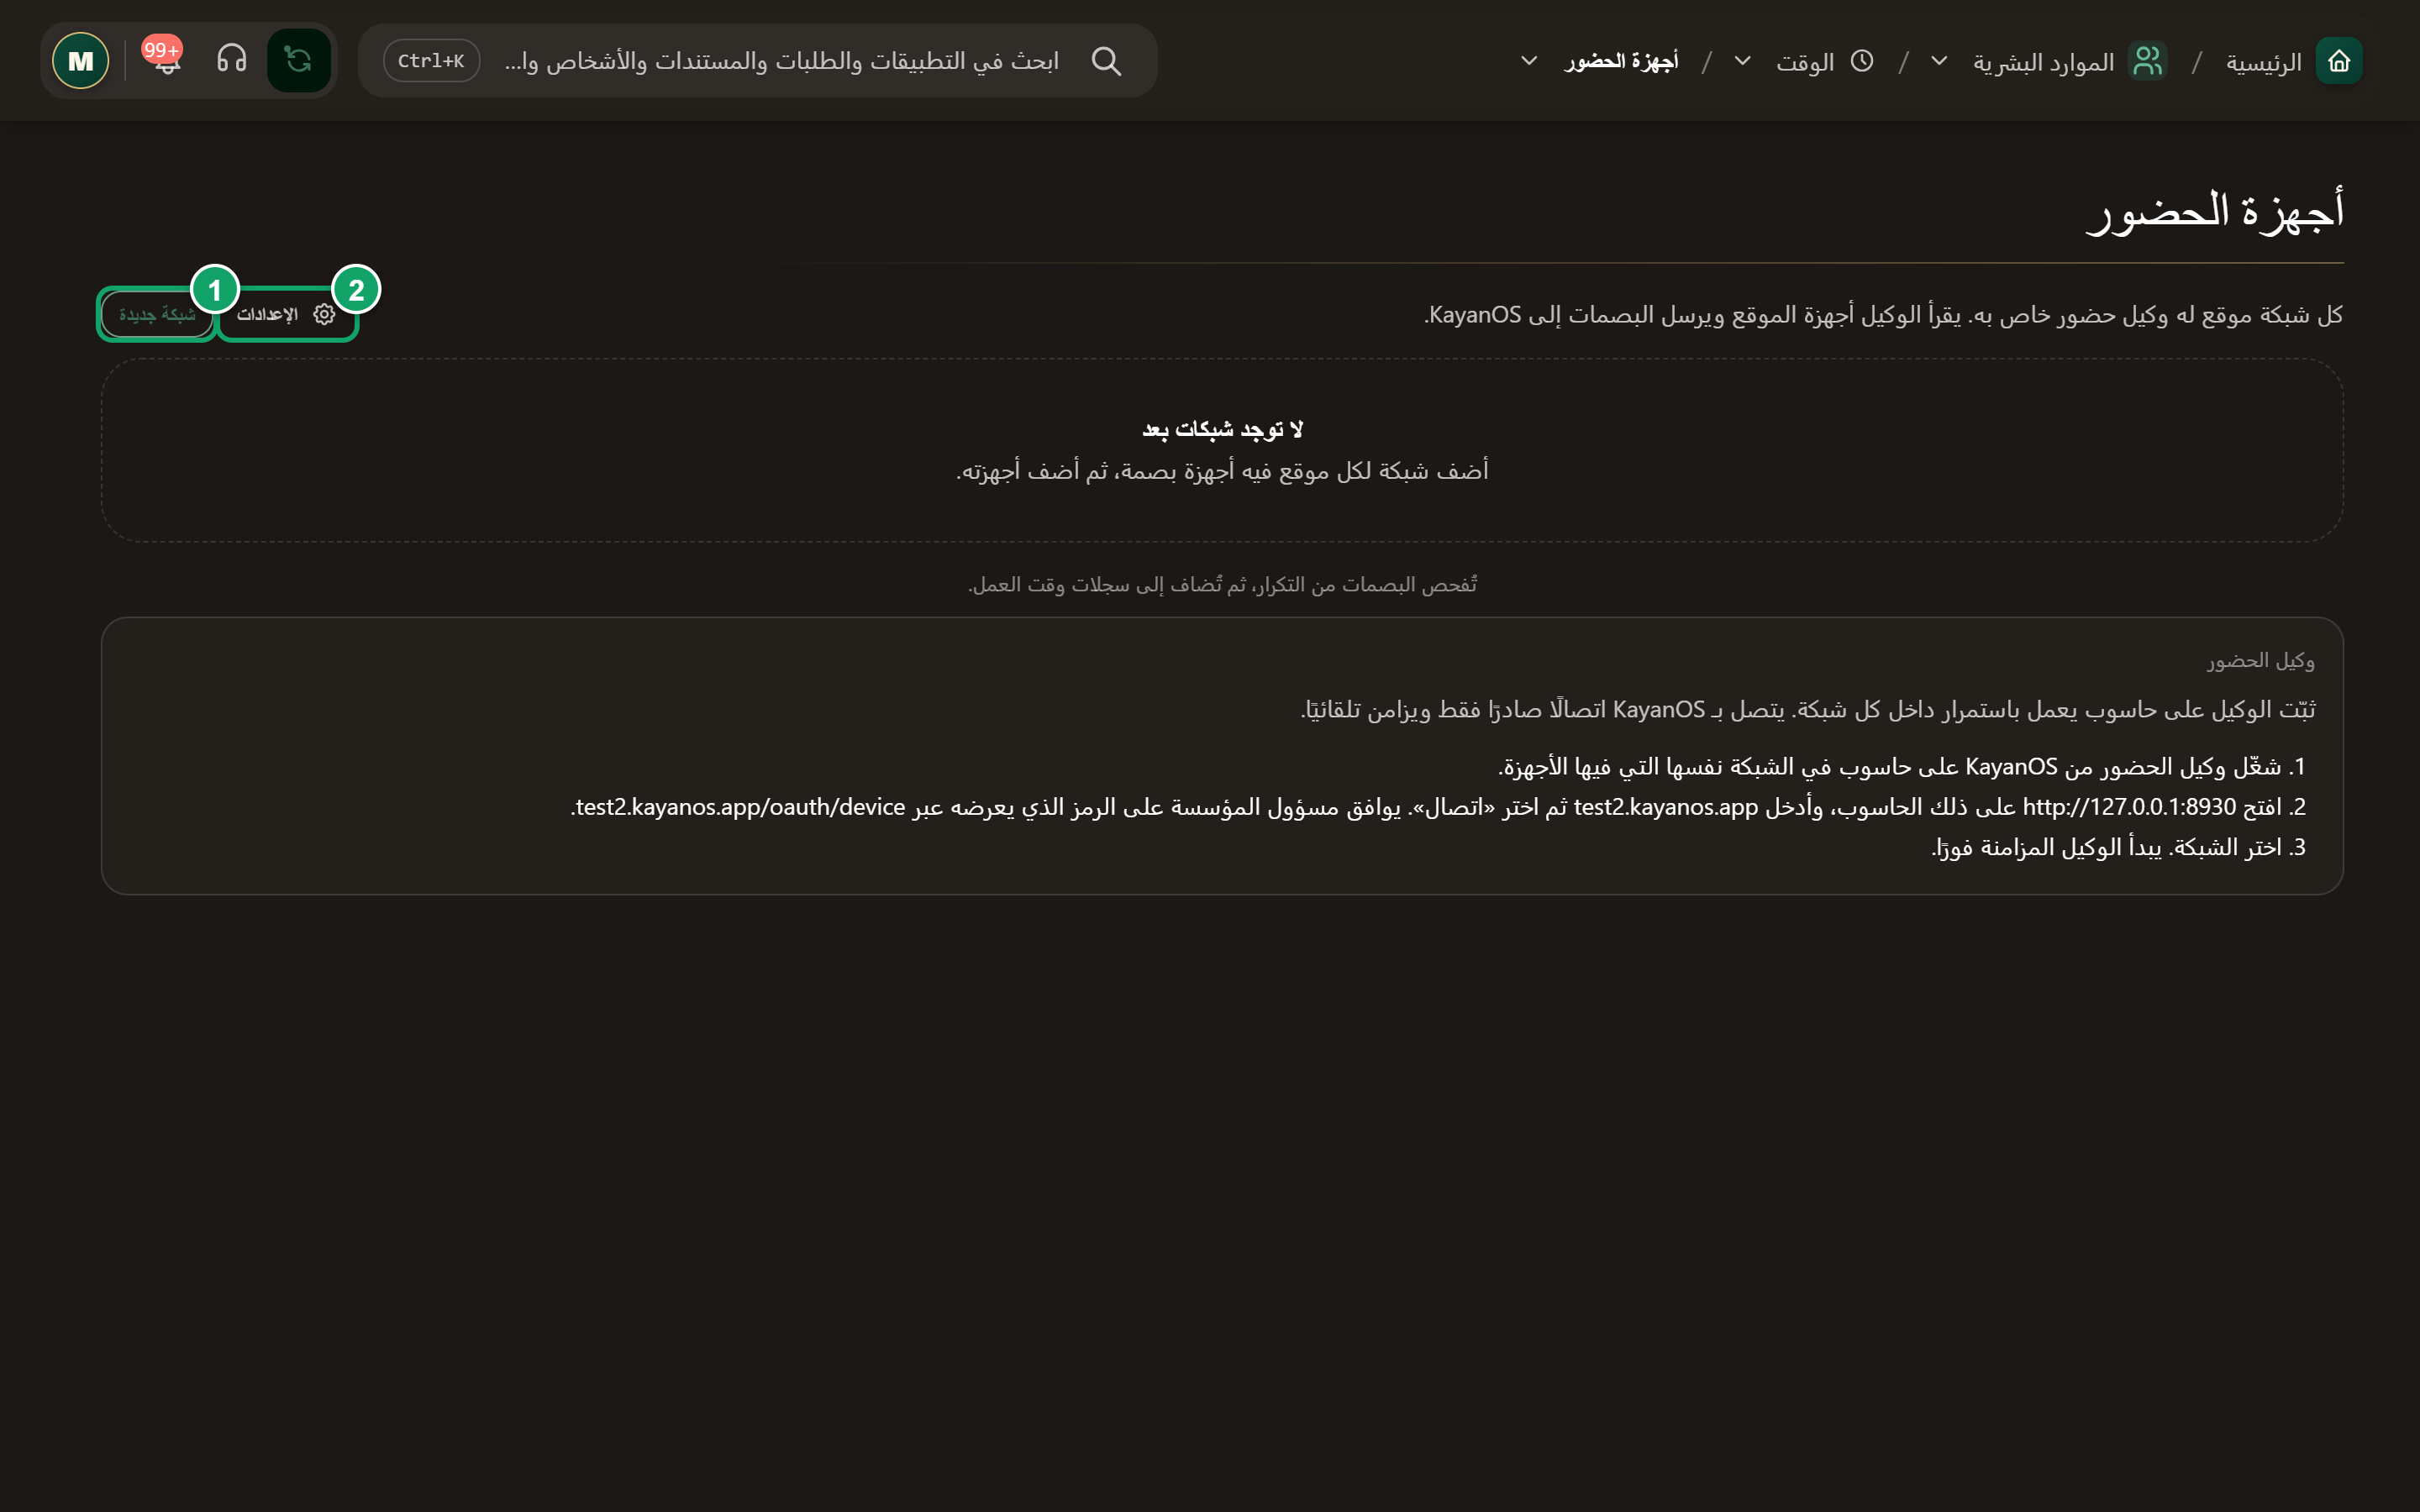
\includegraphics[width=0.95\linewidth]{figures/screens/ch03-feature-attendance-terminals-ar.png}
\caption{أجهزة الحضور: الصفحة كاملة في بيئة الاختبار}
\label{fig:hr-feature-attendance-terminals-screen}
\end{figure}

\begin{table}[H]
\centering
\caption{ما الذي تسجله في أجهزة الحضور؟}
\label{tab:hr-feature-attendance-terminals-data}
\rcZebra
\begin{tabularx}{\linewidth}{R{3.6cm} Y}
\rcHeaderRow
\thh{الجزء} & \thh{ما الذي تضيفه أو تراه؟}\\
الشبكة & الاسم \req{}، الموقع، المنطقة الزمنية، فاصل المزامنة (من \en{5} إلى \en{60} دقيقة).\\
الجهاز & الاسم وعنوان \en{IP} والمنفذ \req{} (\en{4370} افتراضياً)، مفتاح الاتصال، اتجاه البصمة.\\
تفاصيل الجهاز & الطراز، المستخدمون المسجلون، السعة، ساعة الجهاز وفارق توقيتها، آخر بصمة \gen{}.\\
الإعدادات & استيراد البصمات بدءاً من تاريخ، ومطابقة تلقائية برقم الموظف أو يدوية.\\
\end{tabularx}
\end{table}

\subsection{ما الذي يمكنك فعله؟}

\begin{itemize}
  \item «شبكة جديدة»، ثم «إضافة جهاز».
  \item تبويبات الشبكة: الأجهزة، عمليات المزامنة، بصمات غير مطابقة مع «ربط بعضو»، الوكيل مع «قطع اتصال الوكيل».
  \item المزامنة يجريها الوكيل؛ لا يوجد زر مزامنة يدوية.
\end{itemize}

\begin{figure}[H]
\centering
\begin{tikzpicture}[node distance=0.5cm,stepBox/.append style={minimum width=6.5cm,text width=6.1cm,minimum height=0.8cm}]
  \node[stepBox] (a) {\RL{فحص الجهاز}};
  \node[stepBox,below=of a] (b) {\RL{مطابقة المستخدمين}\\\RL{بالأعضاء}};
  \node[stepBox,below=of b] (c) {\RL{مراجعة بصمة حضور}};
  \draw[flowsTo] (a) -- (b);
  \draw[flowsTo] (b) -- (c);
\end{tikzpicture}
\rclegend
\caption{خطوات الاستخدام؛ الأسهم لا تعني معالجة تلقائية}
\label{fig:hr-feature-attendance-terminals-flow}
\end{figure}

\subsection{جرّب وراجع}

\begin{enumerate}
  \item يفتح المسؤول المخوّل «أجهزة الحضور» ثم شبكة الموقع. للموقع الجديد: «شبكة جديدة» ثم «إضافة جهاز».
  \item راجع حالة الوكيل وآخر مزامنة. في «بصمات غير مطابقة» اربط كل مستخدم على الجهاز بالعضو المقابل له.
\end{enumerate}

\textbf{تحقق:} قارن بصمة معروفة بيوم الموظف في حضوري. إن غابت، افحص الوكيل والمطابقة والمنطقة الزمنية.

\clearpage
\section{المستويات الوظيفية}
\label{sec:hr-feature-seniority-levels}

المستوى الوظيفي درجة في سلم الراتب، لها رتبة، وحدّ أدنى وأعلى للراتب، ومجموعة خبرة.

\textbf{متى تفيد؟} مرجع موحد للتعويض: لكل منصب درجة. الدرجة لا تخص موظفاً بعينه، وليست قسيمة راتب. \textbf{المسار:} «الموارد البشرية» / «سلم الراتب» / «المستويات الوظيفية».

\begin{figure}[H]
\centering
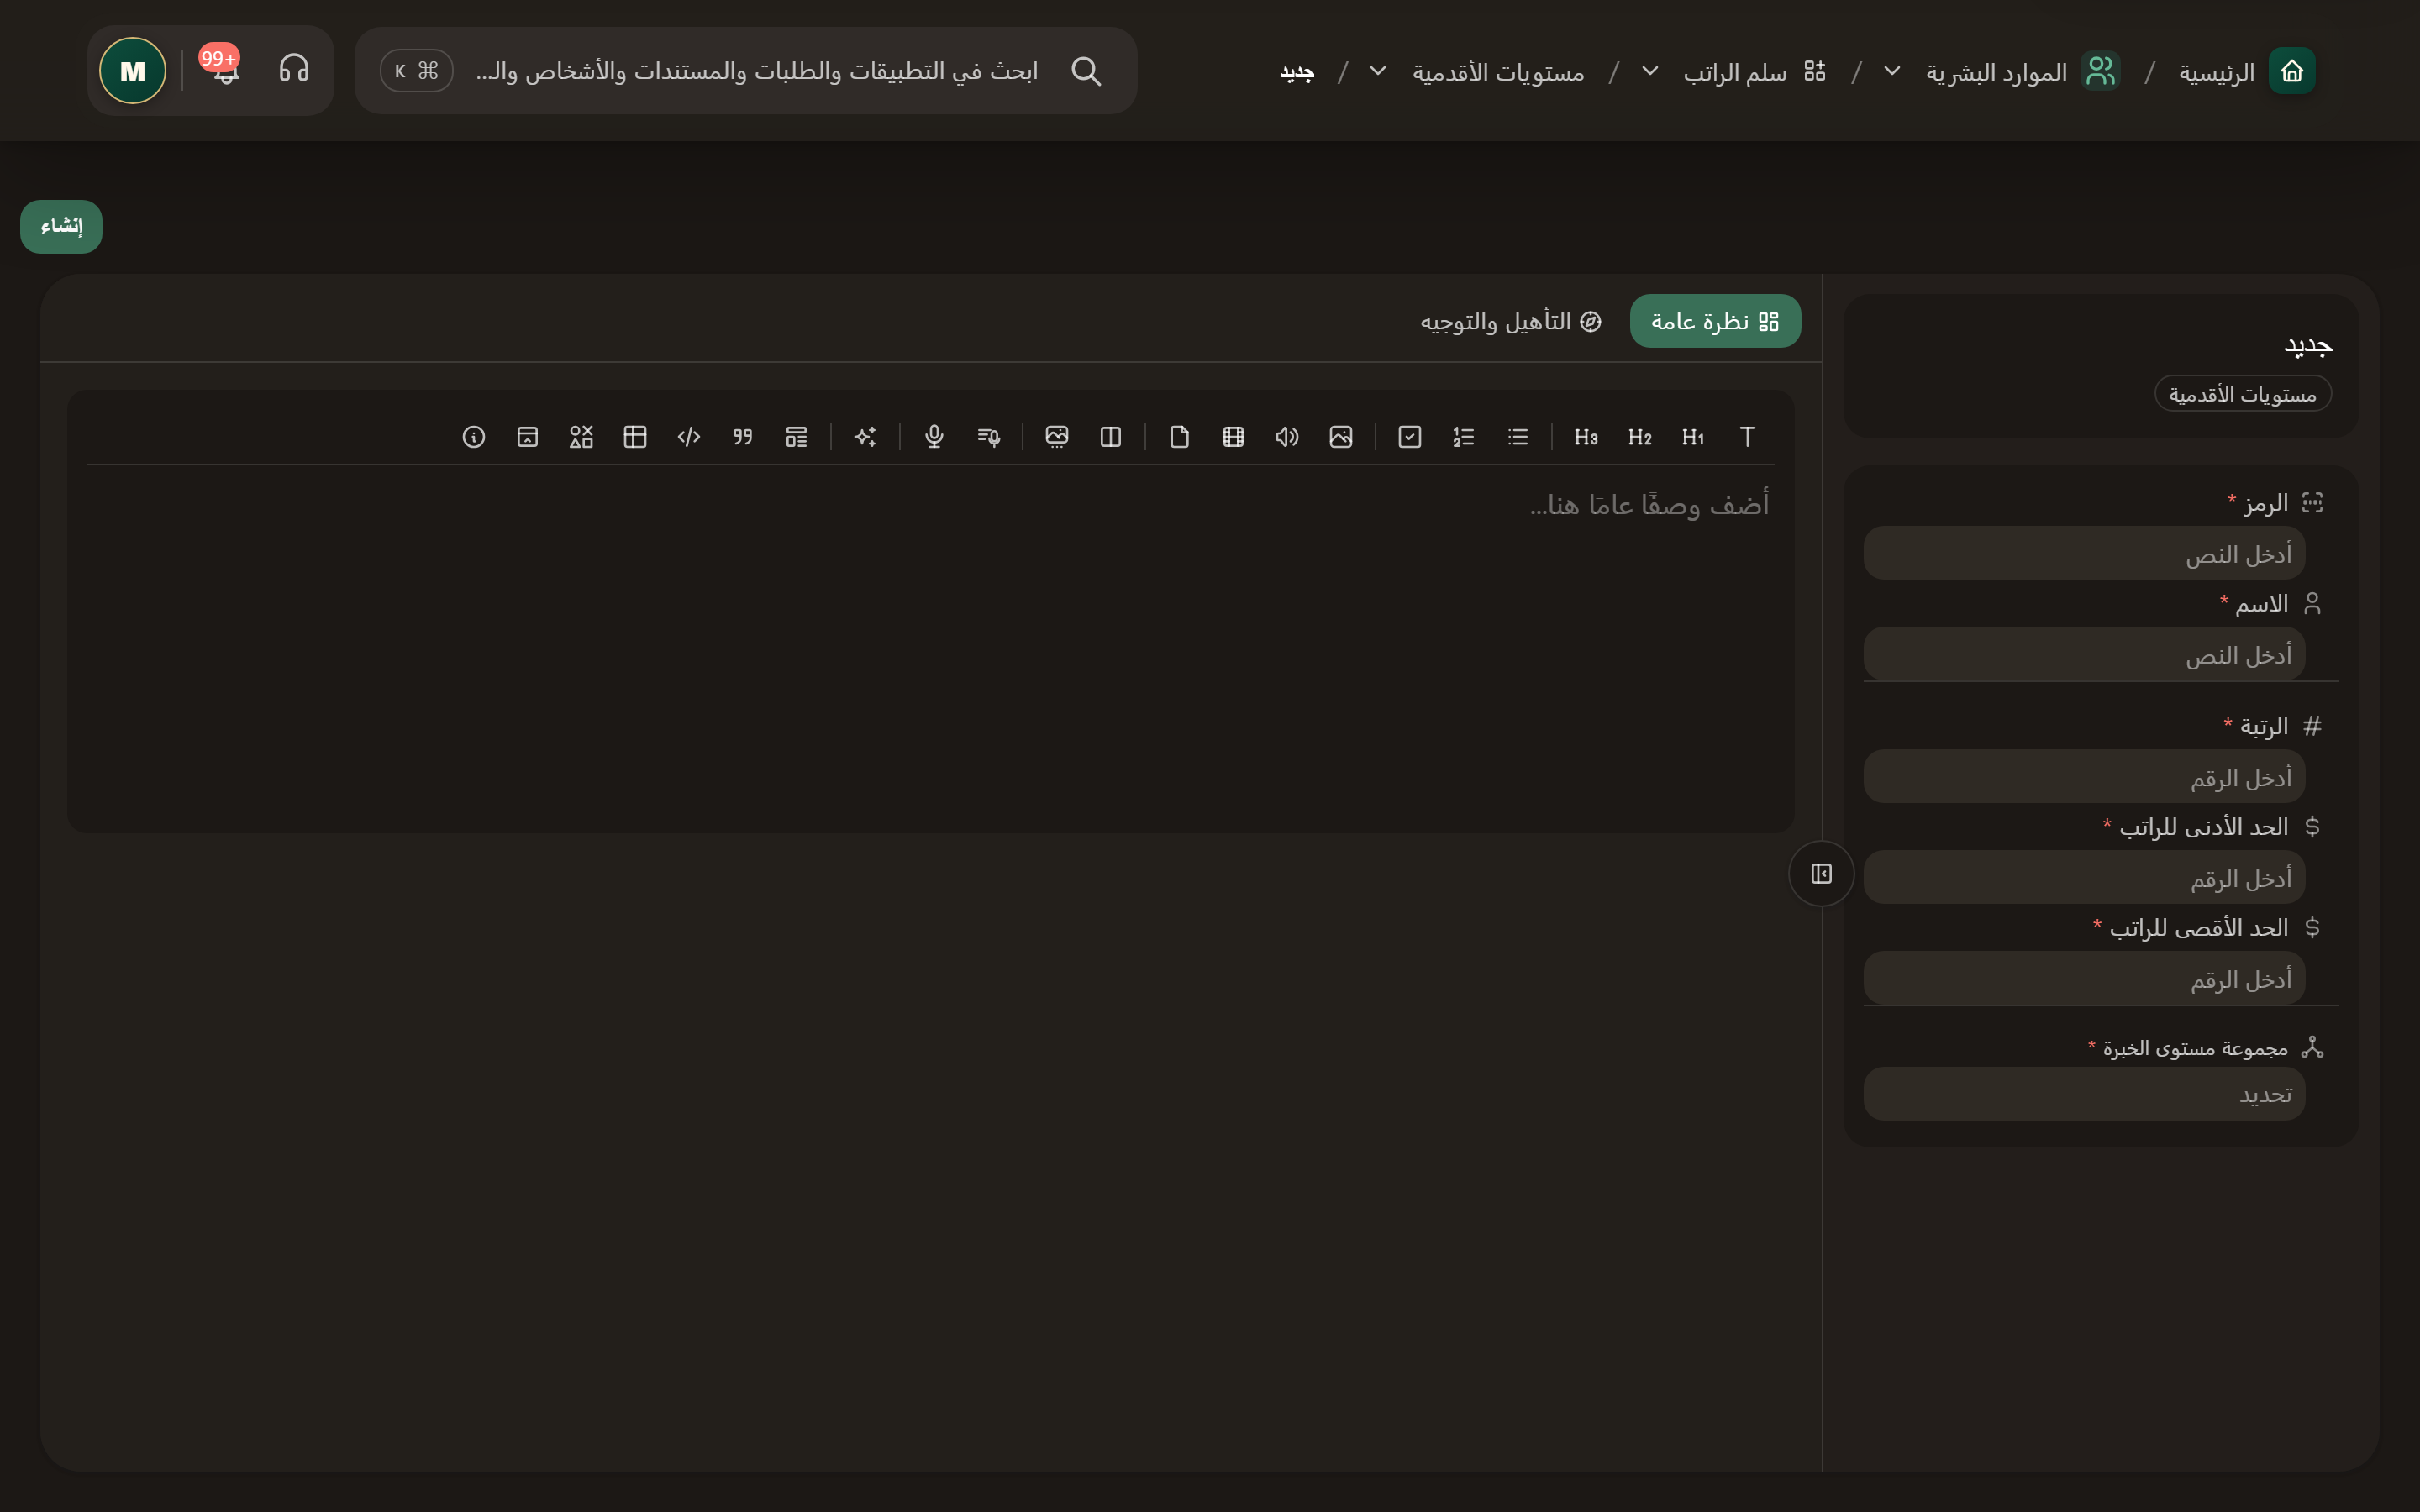
\includegraphics[width=0.95\linewidth]{figures/screens/ch03-feature-seniority-levels-ar.png}
\caption{المستويات الوظيفية: نموذج غير محفوظ في بيئة الاختبار}
\label{fig:hr-feature-seniority-levels-screen}
\end{figure}

\begin{table}[H]
\centering
\caption{ما الذي تسجله في المستوى الوظيفي؟}
\label{tab:hr-feature-seniority-levels-data}
\rcZebra
\begin{tabularx}{\linewidth}{R{3.6cm} Y}
\rcHeaderRow
\thh{الحقل} & \thh{ما الذي تضيفه؟}\\
الاسم والرمز & \req{}؛ الرمز لا يتكرر.\\
الرتبة & \req{}: رقم فريد يرتب الدرجات.\\
الراتب المبدئي والحد الأقصى & \req{}: أدنى راتب في الدرجة وأعلاه.\\
مجموعة مستويات الخبرة & \req{}: الزيادات التي تُضاف إلى الراتب المبدئي.\\
\end{tabularx}
\end{table}

يرتبط المنصب بمستوى وظيفي. يقترح النظام راتب التعيين من الراتب المبدئي وزيادات الخبرة \gen{}.

\begin{figure}[H]
\centering
\begin{tikzpicture}[node distance=0.5cm,stepBox/.append style={minimum width=6.5cm,text width=6.1cm,minimum height=0.8cm}]
  \node[stepBox] (a) {\RL{تعريف الدرجة الوظيفية}};
  \node[stepBox,below=of a] (b) {\RL{مراجعة سلم الراتب}};
  \node[stepBox,below=of b] (c) {\RL{فحص راتب التعيين}};
  \draw[flowsTo] (a) -- (b);
  \draw[flowsTo] (b) -- (c);
\end{tikzpicture}
\rclegend
\caption{خطوات الاستخدام؛ الأسهم لا تعني معالجة تلقائية}
\label{fig:hr-feature-seniority-levels-flow}
\end{figure}

\subsection{جرّب وراجع}

\begin{enumerate}
  \item جهّز مجموعة الخبرة أولاً. افتح «المستويات الوظيفية» وأضف المستوى الوظيفي.
  \item أكمل الاسم والرمز والرتبة والراتب المبدئي والحد الأقصى ومجموعة الخبرة بالقيم المعتمدة، ثم احفظ.
\end{enumerate}

\textbf{تحقق:} افتح «سلم الراتب» وراجع صف الدرجة. اربط الدرجة بالمنصب، ثم راجع راتب التعيين.

\clearpage
\section{مستويات الخبرة}
\label{sec:hr-feature-experience-levels}

تدير في هذه الصفحة مجموعات الخبرة: لكل مجموعة مستويات مرتبة، وقاعدة تزيد الراتب من مستوى إلى المستوى الذي يليه.

\textbf{متى تفيد؟} زيادات خبرة موحدة في سلم الراتب. العبرة بترتيب المستويات؛ تغيير اسم المستوى لا يغير مكانه. \textbf{المسار:} «الموارد البشرية» / «سلم الراتب» / «مستويات الخبرة».

\begin{figure}[H]
\centering
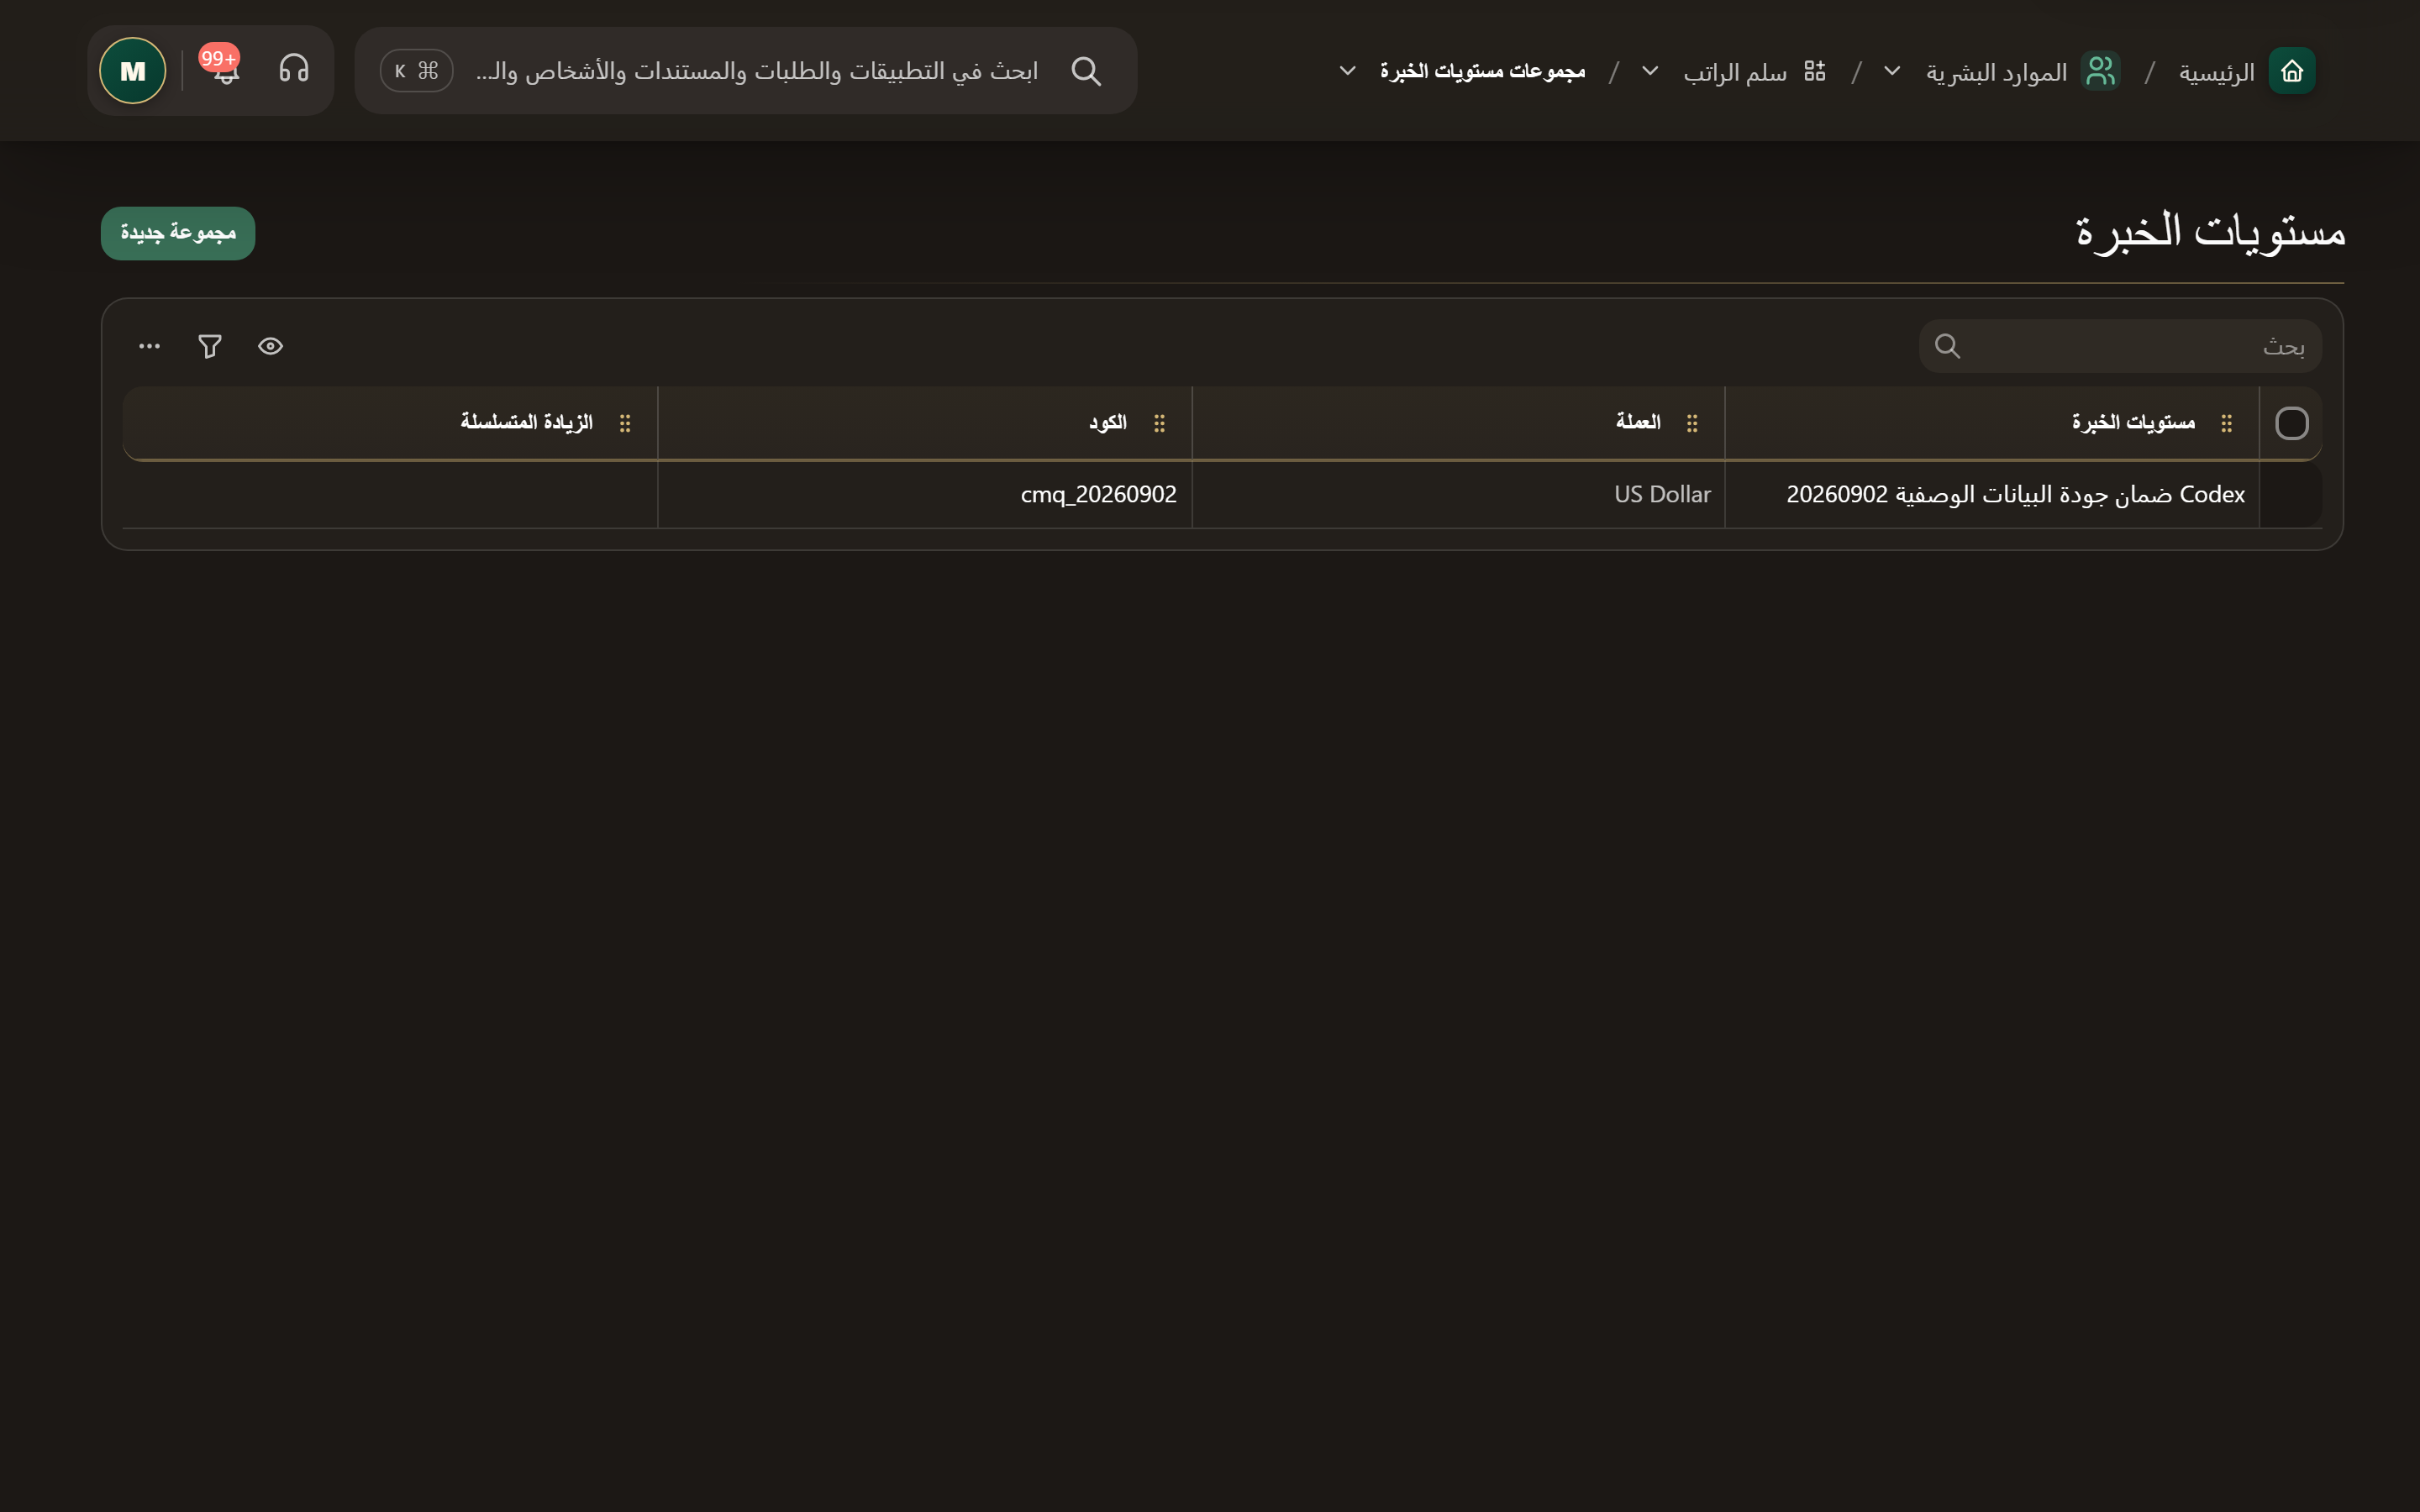
\includegraphics[width=0.95\linewidth]{figures/screens/ch03-feature-experience-levels-ar.png}
\caption{مستويات الخبرة: الصفحة كاملة في بيئة الاختبار}
\label{fig:hr-feature-experience-levels-screen}
\end{figure}

\begin{table}[H]
\centering
\caption{ما الذي تسجله في مجموعة الخبرة؟}
\label{tab:hr-feature-experience-levels-data}
\rcZebra
\begin{tabularx}{\linewidth}{R{3.6cm} Y}
\rcHeaderRow
\thh{التبويب أو الحقل} & \thh{ما الذي تضيفه؟}\\
المجموعة & الاسم والرمز والعملة \req{}.\\
الزيادة المتسلسلة & «قيمة» (مبلغ ثابت) أو «نسبة مئوية».\\
الزيادة الثابتة & عند تفعيلها: الزيادة نفسها بين كل مستوى والمستوى الذي يليه؛ وإلا تُدخل قيمة لكل مستوى.\\
المستويات & الاسم والرمز والوصف لكل مستوى، والترتيب بالسحب والإفلات.\\
\end{tabularx}
\end{table}

\begin{itemize}
  \item «مجموعة جديدة» و«إضافة مستوى». لا يُحذف مستوى مستخدم في تعيينات؛ وتظهر قائمة هذه التعيينات.
\end{itemize}

\begin{figure}[H]
\centering
\begin{tikzpicture}[node distance=0.5cm,stepBox/.append style={minimum width=6.5cm,text width=6.1cm,minimum height=0.8cm}]
  \node[stepBox] (a) {\RL{تعريف مجموعة الخبرة}};
  \node[stepBox,below=of a] (b) {\RL{ترتيب مستوياتها}};
  \node[stepBox,below=of b] (c) {\RL{مراجعة السلم}};
  \draw[flowsTo] (a) -- (b);
  \draw[flowsTo] (b) -- (c);
\end{tikzpicture}
\rclegend
\caption{خطوات الاستخدام؛ الأسهم لا تعني معالجة تلقائية}
\label{fig:hr-feature-experience-levels-flow}
\end{figure}

\subsection{جرّب وراجع}

\begin{enumerate}
  \item افتح «مستويات الخبرة»، ثم «مجموعة جديدة».
  \item أدخل الاسم والرمز والعملة، واختر «قيمة» وفعّل الزيادة الثابتة وأدخل مبلغها. احفظ.
  \item في «المستويات» أضف المستويات ورتّبها من الأقل خبرة إلى الأكثر.
\end{enumerate}

\textbf{تحقق:} افتح «سلم الراتب» وراجع الزيادات. لا تغيّر ترتيب مستويات مشتركة لتعديل راتب شخص واحد.

\clearpage
\section{سلم الراتب}
\label{sec:hr-feature-salary-scale}

سلم الراتب جدول للعرض فقط: لكل درجة وظيفية ومستوى خبرة راتب مرجعي، يحسبه النظام من إعداداتهما.

\textbf{متى تفيد؟} مقارنة الرواتب المرجعية بين الدرجات. المبلغ مرجع للمقارنة، وليس راتباً مستحق الدفع. \textbf{المسار:} «الموارد البشرية» / «سلم الراتب» / «سلم الراتب».

\begin{figure}[H]
\centering
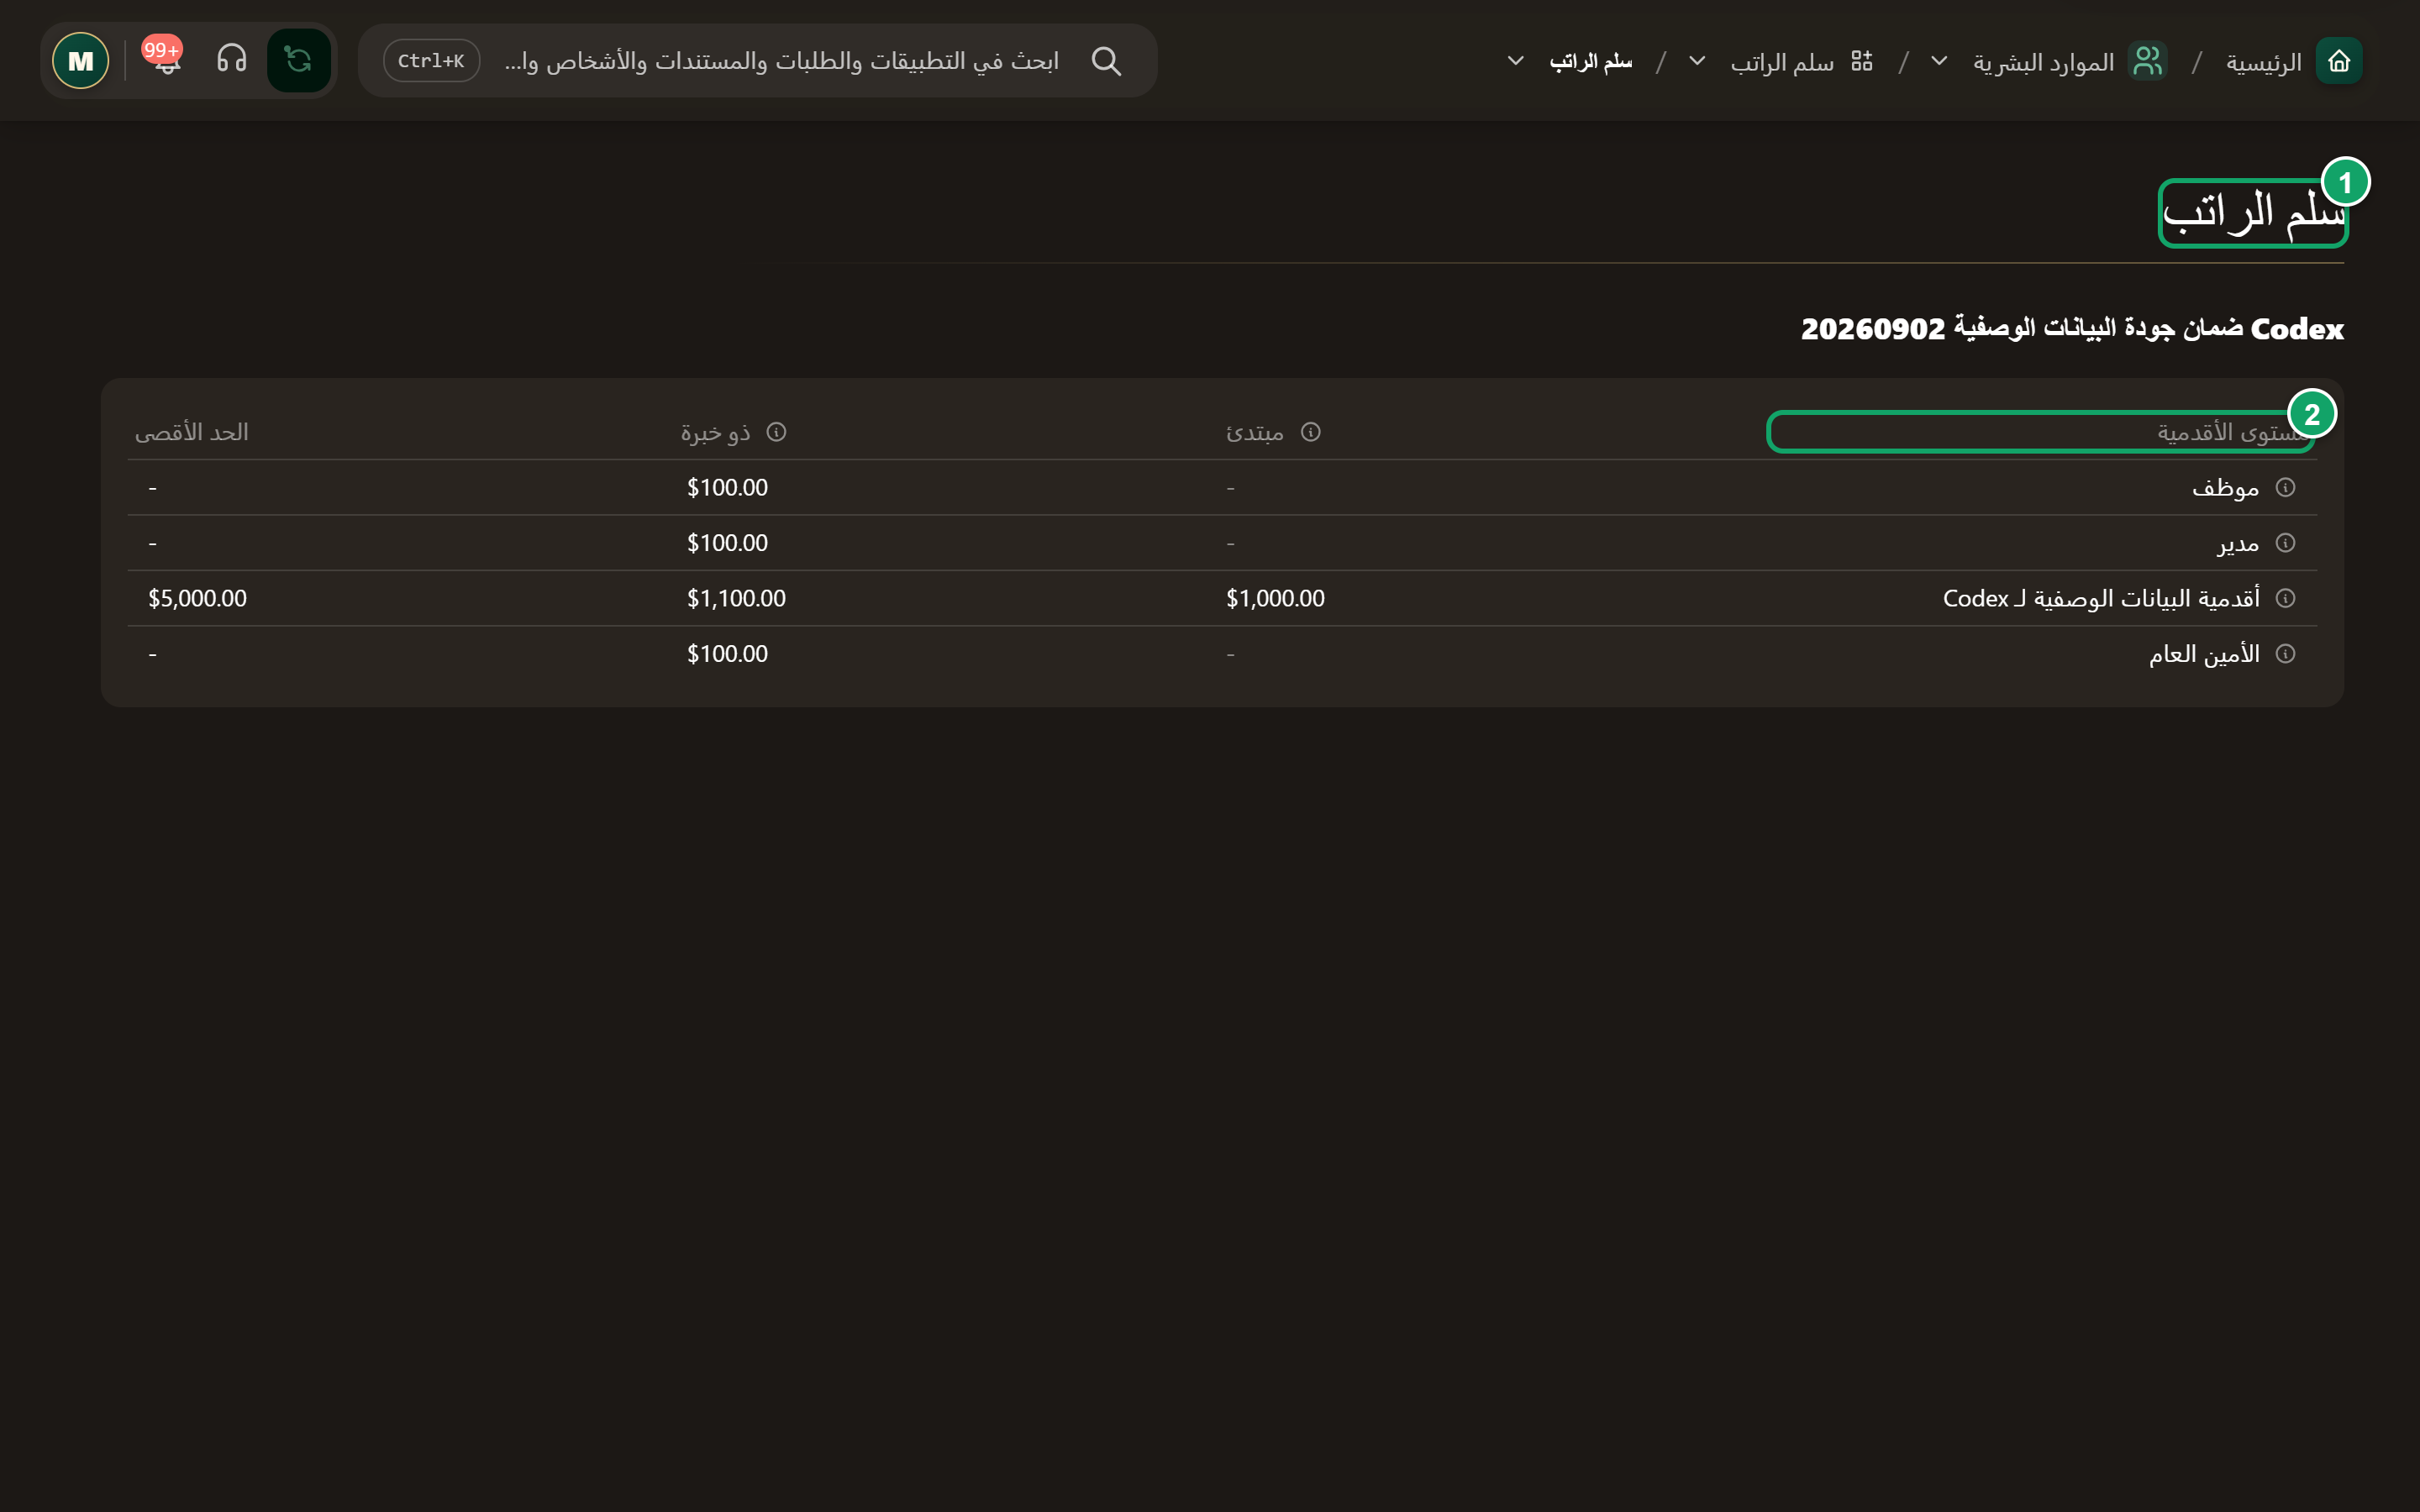
\includegraphics[width=0.95\linewidth]{figures/screens/ch03-feature-salary-scale-ar.png}
\caption{سلم الراتب: الصفحة كاملة في بيئة الاختبار}
\label{fig:hr-feature-salary-scale-screen}
\end{figure}

\begin{table}[H]
\centering
\caption{كيف تقرأ سلم الراتب؟}
\label{tab:hr-feature-salary-scale-data}
\rcZebra
\begin{tabularx}{\linewidth}{R{3.6cm} Y}
\rcHeaderRow
\thh{الجزء} & \thh{ماذا يعني؟}\\
جدول لكل مجموعة & كل مجموعة خبرة لها جدولها وعملتها.\\
الصفوف & المستويات الوظيفية، من الرتبة الأعلى إلى الأدنى.\\
الأعمدة & مستويات الخبرة بترتيبها، والعمود الأخير الحد الأقصى.\\
الخلية & الراتب المبدئي مع زيادات الخبرة حتى هذا المستوى \gen{}.\\
\end{tabularx}
\end{table}

لا يُعدَّل السلم مباشرة؛ غيّر المستويات الوظيفية أو مستويات الخبرة.

\begin{figure}[H]
\centering
\begin{tikzpicture}[node distance=0.4cm,stepBox/.append style={minimum width=6cm,text width=5.6cm,minimum height=0.7cm}]
  \node[stepBox] (s0) {\RL{مستويات الخبرة:}\\\RL{المجموعة والزيادات}};
  \node[stepBox,below=of s0] (s1) {\RL{المستويات الوظيفية:}\\\RL{الرواتب والرتب}};
  \node[stepBox,below=of s1] (s2) {\RL{سلم الراتب: راجع}\\\RL{الخلايا}};
  \node[stepBox,below=of s2] (s3) {\RL{التعيين: راجع الراتب}\\\RL{والعملة}};
  \draw[flowsTo] (s0) -- (s1);
  \draw[flowsTo] (s1) -- (s2);
  \draw[flowsTo] (s2) -- (s3);
\end{tikzpicture}
\rclegend
\caption{إن كانت مؤسستك تستخدم سلم الراتب}
\label{fig:hr-scale-setup}
\end{figure}

\subsection{جرّب وراجع}

\begin{enumerate}
  \item جهّز مجموعة الخبرة ومستوياتها، ثم المستويات الوظيفية. افتح «سلم الراتب».
  \item ابحث عن الدرجة ومستوى الخبرة وراجع الخلية. إن كانت غير متوقعة، افحص الراتب المبدئي والزيادة.
\end{enumerate}

\textbf{تحقق:} قارن المبلغ المرجعي براتب تعيين سارة وعملته. تبيّن الأسهم ترتيب الإعداد، ولا تعني دفع الراتب تلقائياً.

\clearpage
\section{مدخلات الرواتب}
\label{sec:hr-feature-payroll-inputs}

مدخل الراتب بند متغير لشهر محدد، مثل مكافأة أو خصم أو عمل إضافي، يُسجَّل على تعيين موظف.

\textbf{متى تفيد؟} كل مبلغ استثنائي مسجل وقابل للتتبع، بدلاً من تعديل الراتب يدوياً. \textbf{المسار:} «الموارد البشرية» / «الدفع» / «مدخلات الرواتب».

\begin{figure}[H]
\centering
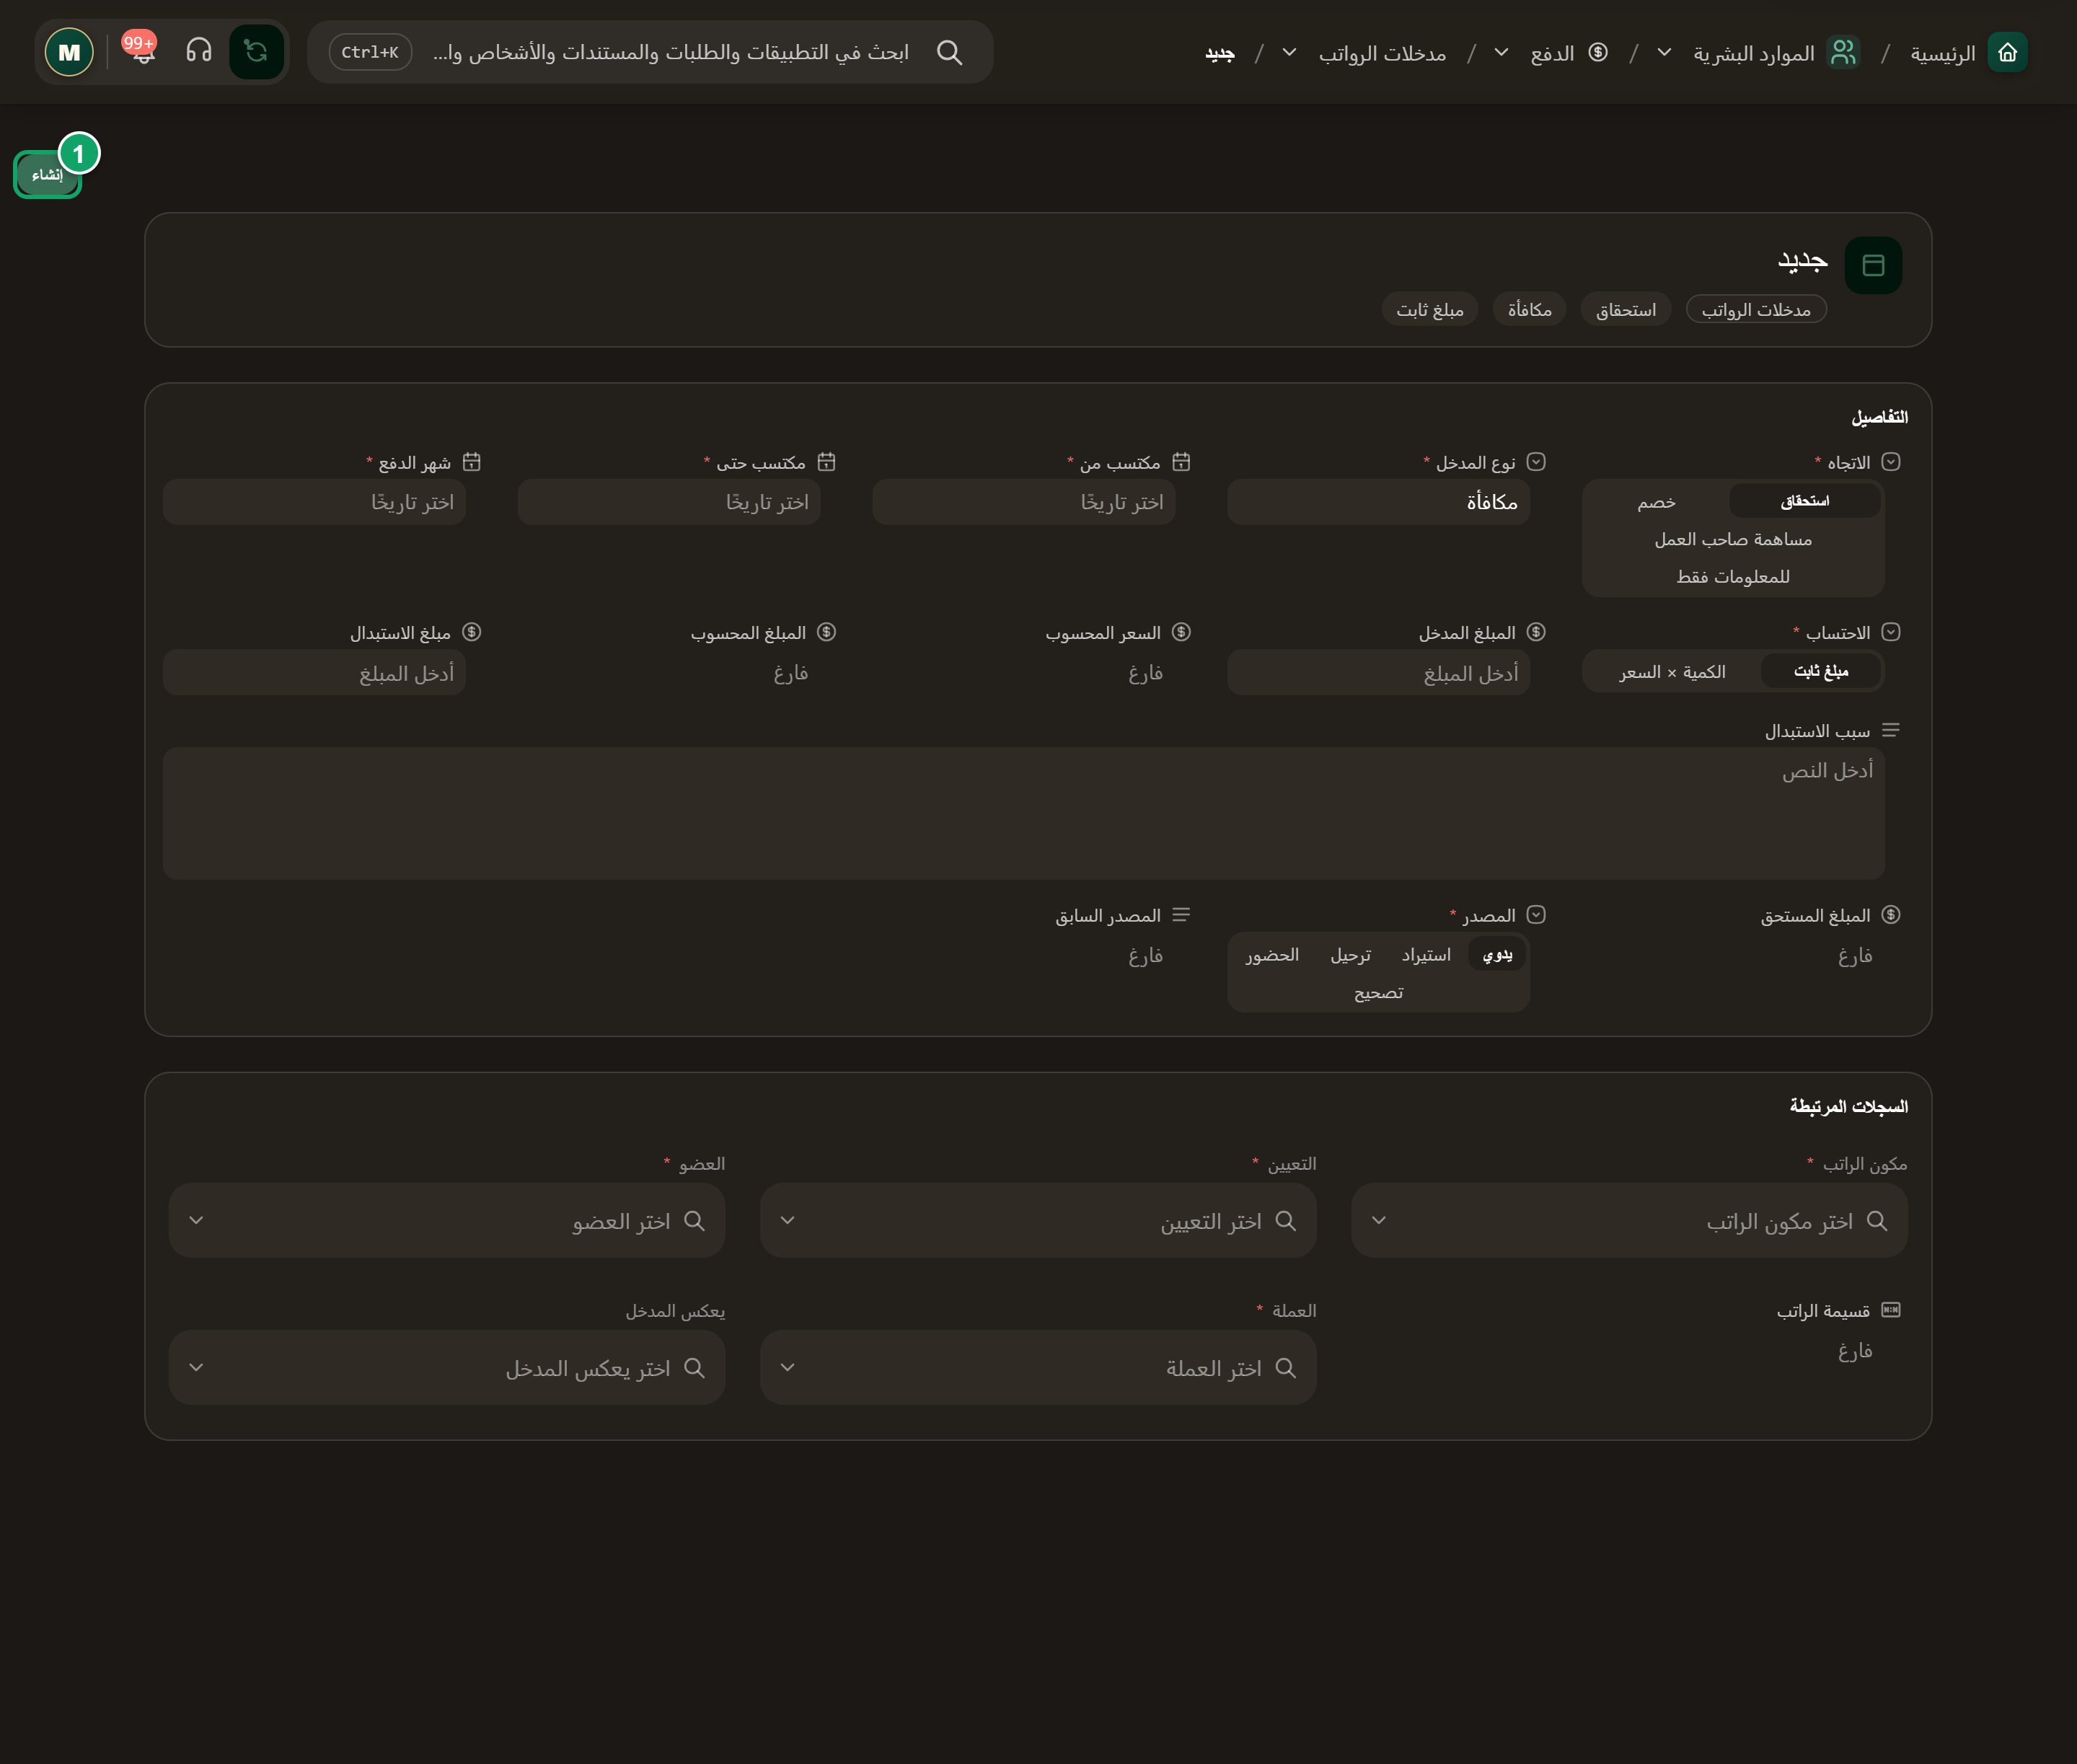
\includegraphics[width=0.95\linewidth]{figures/screens/ch03-payroll-input-fields-ar.png}
\caption{مدخلات الرواتب: أكمل الحقول المعلّمة بـ*؛ لم يُحفظ}
\label{fig:hr-feature-payroll-inputs-screen}
\end{figure}

\begin{table}[H]
\centering
\caption{ما الذي تسجله في مدخل الراتب؟}
\label{tab:hr-feature-payroll-inputs-data}
\rcZebra
\begin{tabularx}{\linewidth}{R{3.6cm} Y}
\rcHeaderRow
\thh{الحقل} & \thh{ما الذي تضيفه؟}\\
الاتجاه ونوع المدخل & \req{}: الاتجاه: استحقاق أو خصم أو مساهمة صاحب العمل أو للمعلومات فقط؛ النوع: مكافأة، خصم، عمل إضافي، رد مصروف، تسوية.\\
المكون والتعيين والعضو & \req{}: مكون الراتب، والعضو وتعيينه.\\
الفترة & مكتسب من وحتى، وشهر الدفع \req{}.\\
الاحتساب & مبلغ ثابت، أو الكمية × السعر؛ وفي العمل الإضافي: الساعات وتصنيف الوقت: نهاري، ليلي، يوم الراحة، العطلة.\\
الاستبدال & مبلغ بديل يحل محل المحسوب، وسببه \opt{}.\\
النتيجة & السعر والمبلغ المحسوب والمبلغ المستحق وتفاصيل الاحتساب \gen{}.\\
\end{tabularx}
\end{table}

\subsection{ما الذي يمكنك فعله؟}

\begin{itemize}
  \item «معاينة الاحتساب» تحسب المبلغ من سياسة الرواتب وشروط التعويض.
  \item يُقفل المدخل عند اعتماد قسيمة تستخدمه. للتصحيح بعدها أضف مدخلاً جديداً واختر المدخل الأصلي في «يعكس المدخل».
\end{itemize}

\begin{figure}[H]
\centering
\begin{tikzpicture}[node distance=0.5cm,stepBox/.append style={minimum width=6.5cm,text width=6.1cm,minimum height=0.8cm}]
  \node[stepBox] (a) {\RL{تسجيل البند المعتمد}};
  \node[stepBox,below=of a] (b) {\RL{معاينة حسابه}};
  \node[stepBox,below=of b] (c) {\RL{مراجعة قسيمة الراتب}};
  \draw[flowsTo] (a) -- (b);
  \draw[flowsTo] (b) -- (c);
\end{tikzpicture}
\rclegend
\caption{خطوات الاستخدام؛ الأسهم لا تعني معالجة تلقائية}
\label{fig:hr-feature-payroll-inputs-flow}
\end{figure}

\subsection{جرّب وراجع}

\begin{enumerate}
  \item بعد مراجعة الوقت والإجازات، افتح «مدخلات الرواتب» وابحث عن البند لتجنب تكراره.
  \item أضف: «استحقاق»، «مكافأة»، المكون، تعيين سارة، الفترة وشهر الدفع، «مبلغ ثابت» والمبلغ المعتمد. احفظ.
  \item افتح «معاينة الاحتساب» وراجع المبلغ المستحق.
\end{enumerate}

\textbf{تحقق:} يظهر المبلغ في قسيمة سارة بعد «احتساب». المعاينة ليست دفعاً.

\clearpage
\section{قسائم الرواتب}
\label{sec:hr-feature-salary-slips}

قسيمة الراتب حساب راتب موظف لفترة: أيامه ومستحقاته وخصوماته وصافي راتبه. وحالاتها: مسودة، محسوبة، معتمدة.

\textbf{متى تفيد؟} راجع حساب سارة الفردي قبل إعداد كشف الرواتب، لتتبّع كل مبلغ إلى بنده. \textbf{المسار:} «الموارد البشرية» / «الدفع» / «قسائم الرواتب».

\begin{figure}[H]
\centering
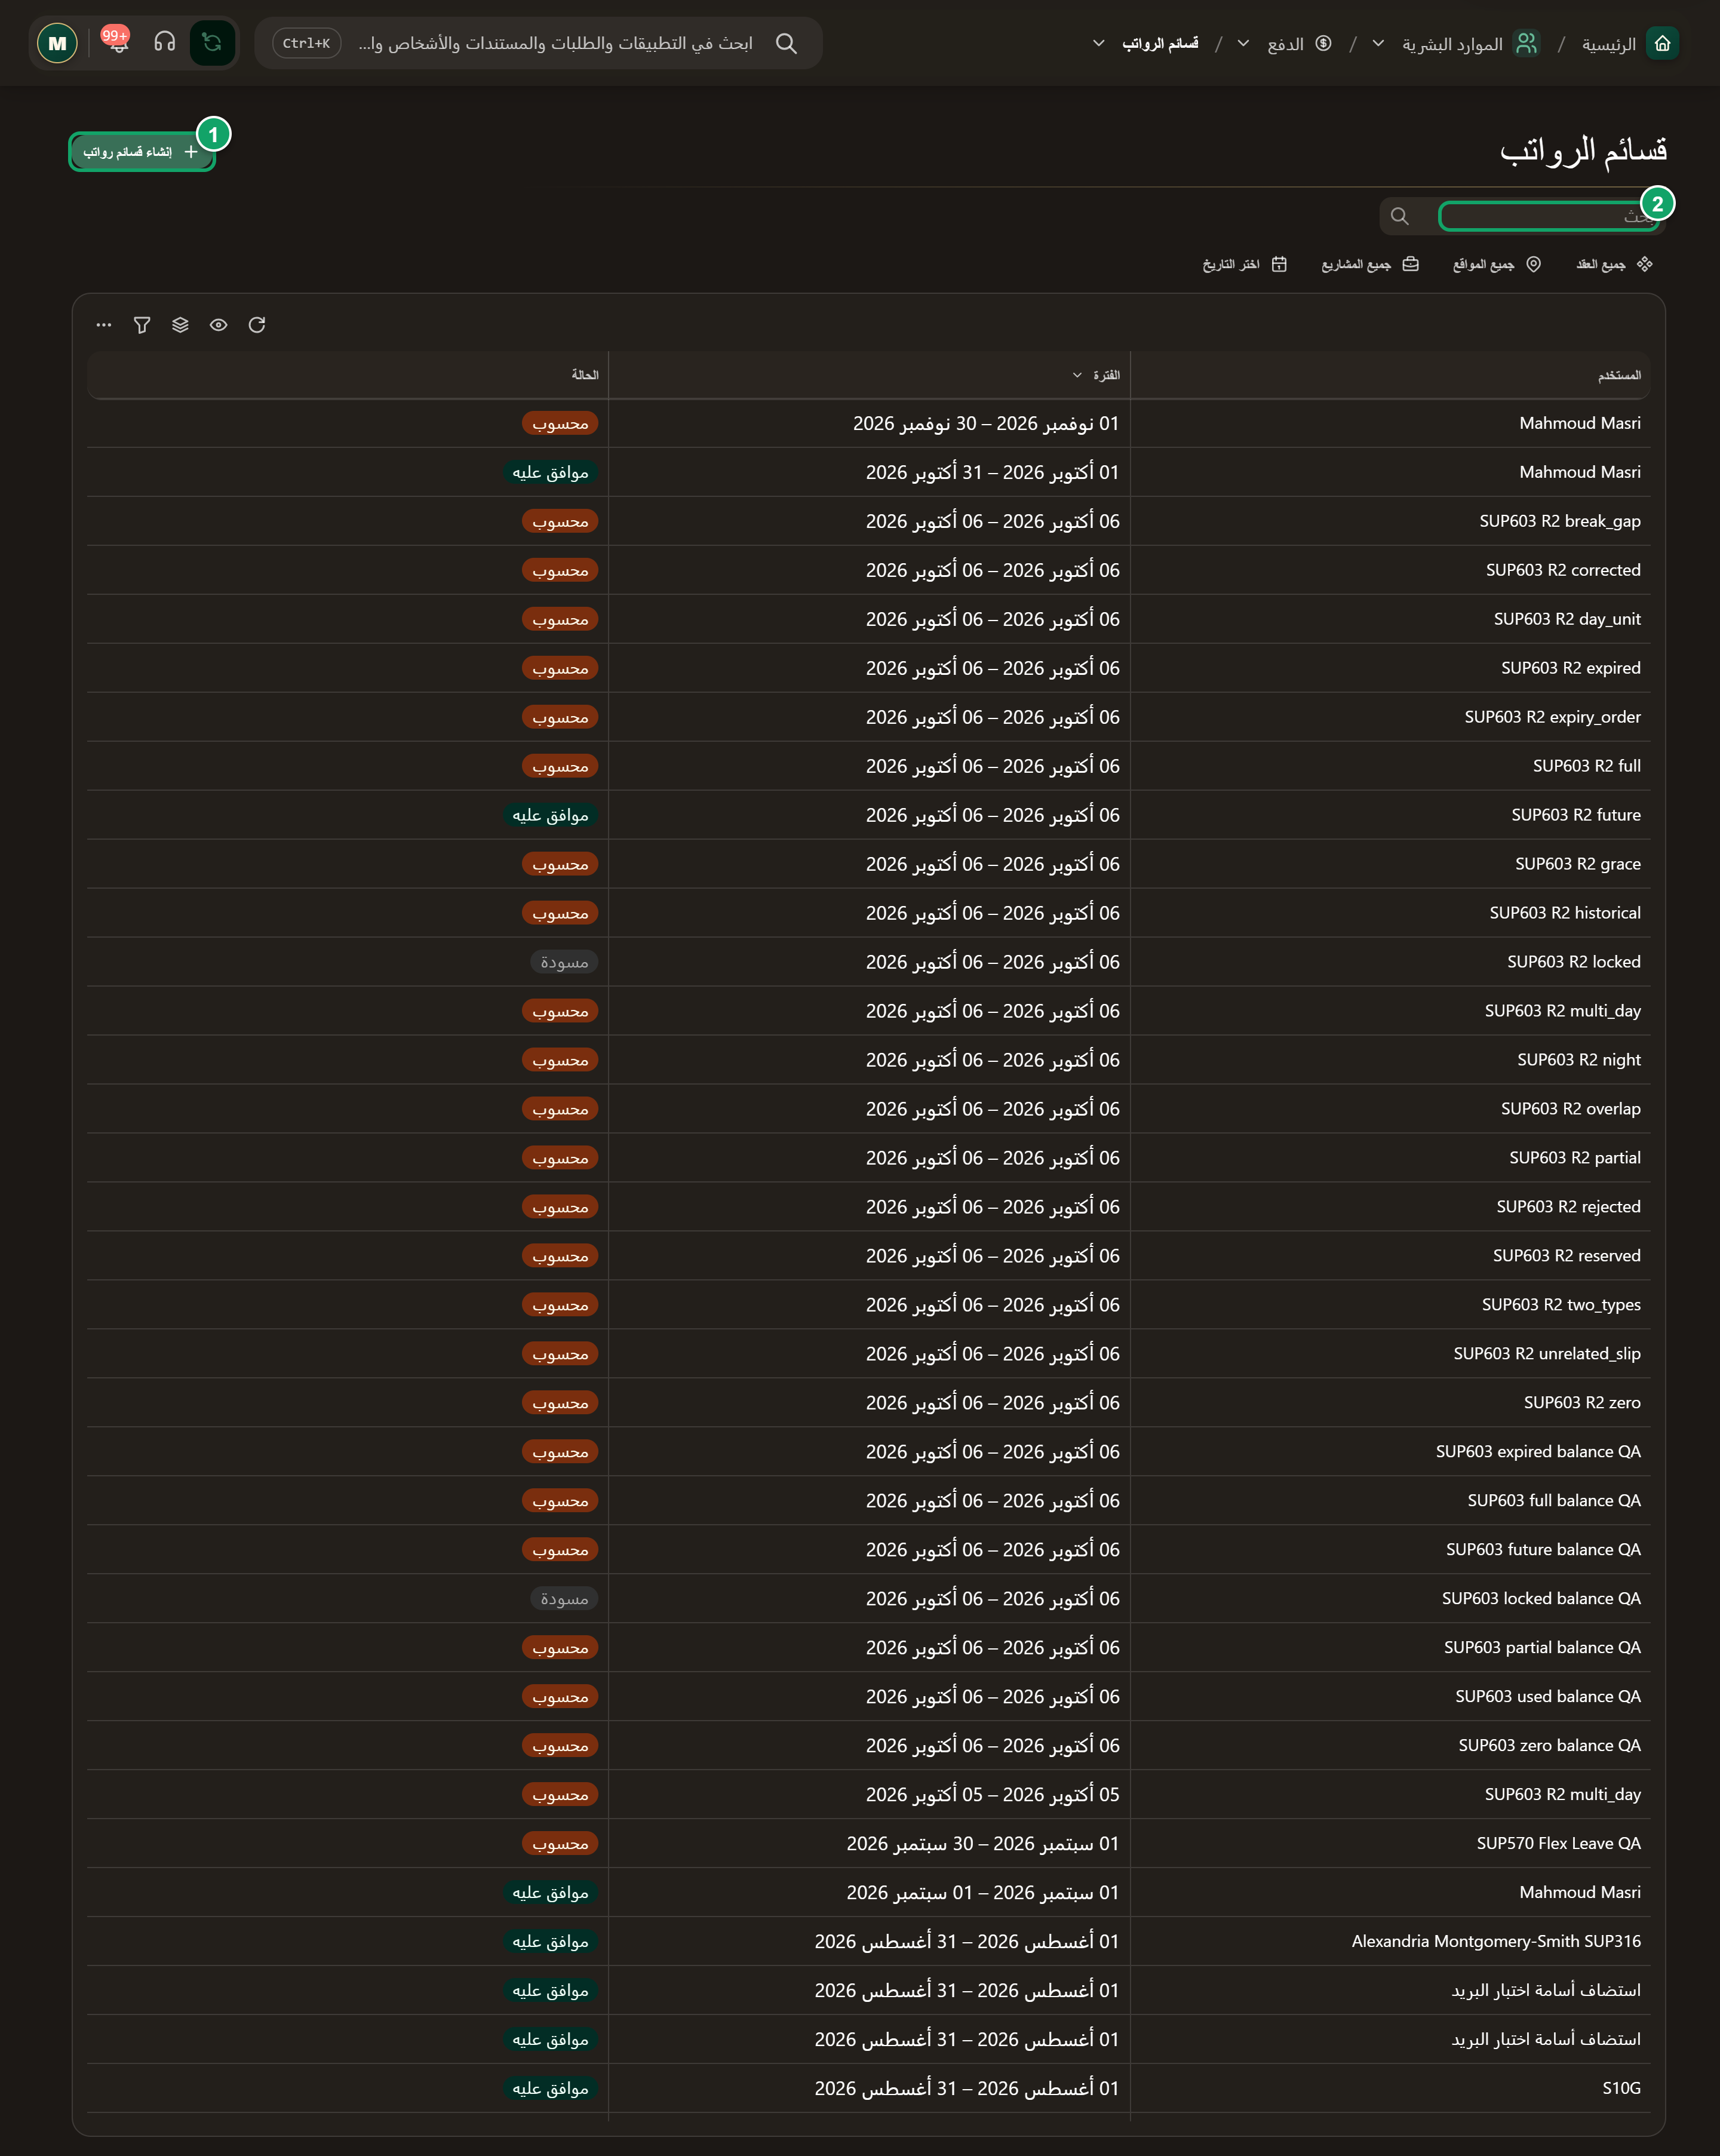
\includegraphics[width=0.95\linewidth]{figures/screens/ch03-create-slips-clear-ar.png}
\caption{قسائم الرواتب: الصفحة كاملة قبل إنشاء القسائم}
\label{fig:hr-feature-salary-slips-screen}
\end{figure}

\begin{table}[H]
\centering
\caption{ما الذي تعرضه القسيمة؟}
\label{tab:hr-feature-salary-slips-data}
\rcZebra
\begin{tabularx}{\linewidth}{R{3.6cm} Y}
\rcHeaderRow
\thh{القسم} & \thh{ماذا يعرض؟}\\
معلومات الموظف & الاسم والمنصب والموقع وبداية العقد ونهايته.\\
ملخص الدفع & الفترة، أيام العمل، العملة، الراتب الأساسي للفترة.\\
الأيام & أيام العمل والعطل والإجازات المدفوعة وغير المدفوعة والعمل الإضافي.\\
حساب الراتب & بند لكل مصدر بمعادلته، ثم المبلغ المستحق والتقريب وإجمالي الراتب الصافي.\\
المشاريع والملاحظات & نسبة كل مشروع ومبلغه، وملاحظات القسيمة.\\
\end{tabularx}
\end{table}

\begin{itemize}
  \item التصفية بالاسم والوحدات والمواقع والمشاريع والشهر.
  \item «احتساب» ثم «إعادة الاحتساب»، و«اعتماد»، و«حذف» القسيمة المسودة أو المحسوبة. القسيمة المعتمدة لا تُعدّل.
\end{itemize}

\begin{figure}[H]
\centering
\begin{tikzpicture}[node distance=0.4cm,stepBox/.append style={minimum width=6.5cm,text width=6.1cm,minimum height=0.7cm}]
  \node[stepBox] (m0) {\RL{التعيين وبيانات}\\\RL{الموظف}};
  \node[stepBox,below=of m0] (m1) {\RL{مراجعة الدوام}\\\RL{والإجازات}};
  \node[stepBox,below=of m1] (m2) {\RL{مراجعة مدخلات}\\\RL{الرواتب}};
  \node[stepBox,below=of m2] (m3) {\RL{احتساب قسيمة الراتب}\\\RL{واعتمادها}};
  \node[stepBox,below=of m3] (m4) {\RL{توليد كشف الرواتب}\\\RL{ومراجعته}};
  \draw[flowsTo] (m0) -- (m1);
  \draw[flowsTo] (m1) -- (m2);
  \draw[flowsTo] (m2) -- (m3);
  \draw[flowsTo] (m3) -- (m4);
\end{tikzpicture}
\rclegend
\caption{مسار المراجعة من الموظف إلى كشف الرواتب}
\label{fig:hr-review-flow}
\end{figure}

\subsection{جرّب وراجع}

\begin{enumerate}
  \item افتح «قسائم الرواتب»، ثم «إنشاء قسائم رواتب».
  \item اختر «نهاية الفترة»، ثم حدّد صفّ سارة ومنصبها. راجع «بداية الفترة»؛ تبدأ أول قسيمة من تاريخ بدء التعيين، ويمكنك تعديل التاريخ.
  \item أنشئ المسودة بالزر الذي يعرض عدد المحددين، ثم افتح قسيمتها. إن وُجدت مسودة، راجعها أو احذفها بدلاً من إنشاء نسخة مكررة.
  \item اختر «احتساب». راجع الأيام والبنود والصافي. بعد تغيير المدخلات اختر «إعادة الاحتساب».
  \item عند صحة البنود اختر «اعتماد» وأكّد. الاعتماد يُقفل مدخلات الرواتب المستخدمة فيها.
\end{enumerate}

\textbf{تحقق:} تظهر حالة القسيمة «معتمد» في القائمة. الاعتماد لا يعني أن الراتب دُفع.

\clearpage
\section{كشوف الرواتب}
\label{sec:hr-feature-payrolls}

كشف الرواتب يجمع القسائم المعتمدة لشهر في كشف واحد، بإجمالي لكل عضو ولكل مشروع.

\textbf{متى تفيد؟} بعد فحص القسائم، لمراجعة رواتب الشهر واعتمادها وتصديرها. \textbf{المسار:} «الموارد البشرية» / «الدفع» / «كشوف الرواتب».

\begin{figure}[H]
\centering
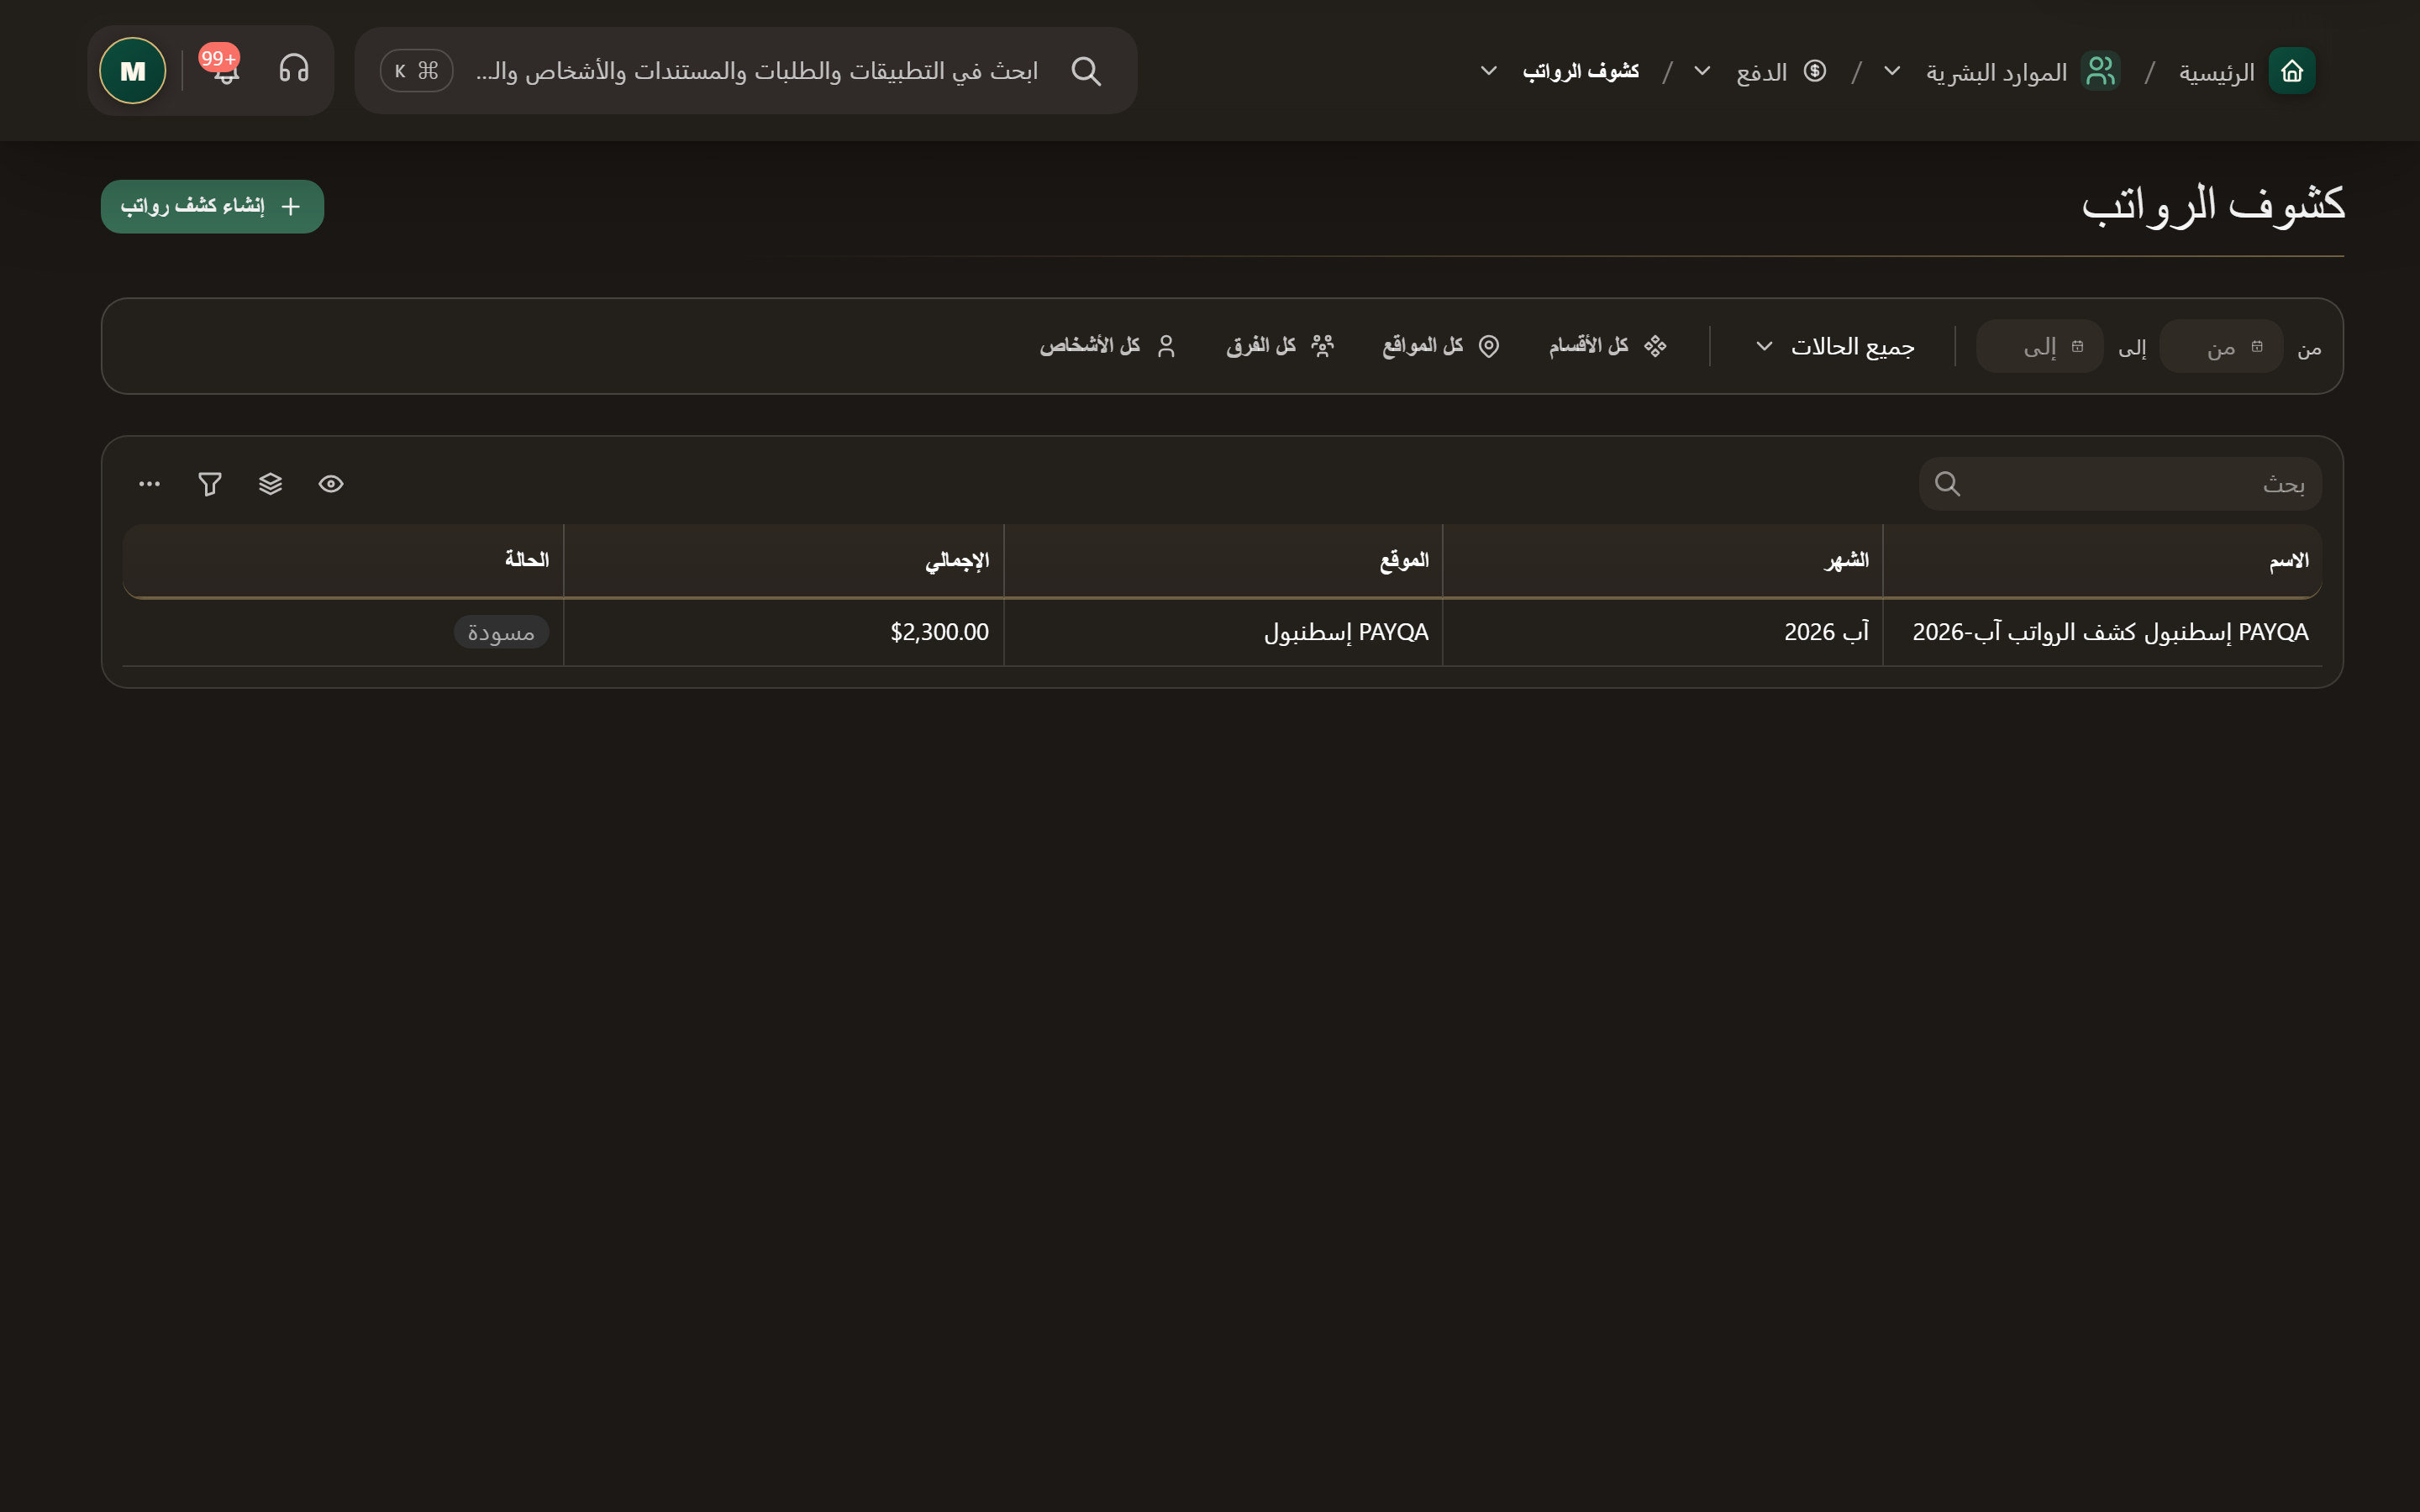
\includegraphics[width=0.95\linewidth]{figures/screens/ch03-feature-payrolls-ar.png}
\caption{كشوف الرواتب: الصفحة كاملة في بيئة الاختبار}
\label{fig:hr-feature-payrolls-screen}
\end{figure}

\begin{table}[H]
\centering
\caption{ما الذي يضمه كشف الرواتب؟}
\label{tab:hr-feature-payrolls-data}
\rcZebra
\begin{tabularx}{\linewidth}{R{3.6cm} Y}
\rcHeaderRow
\thh{الجزء} & \thh{ماذا يعرض؟}\\
الإنشاء & الشهر والسنة؛ المصدر: القسائم المعتمدة أو جميع الأعضاء؛ والتصفية بالأقسام والمواقع والفرق والأشخاص.\\
القائمة & الاسم والشهر والموقع والإجمالي والحالة: مسودة أو معتمد.\\
المدفوعات & لكل عضو أو لكل مشروع: أيام العمل، المكافآت، الخصومات، الصافي، المبلغ المستحق، الملاحظات.\\
المشاريع & نسبة كل مشروع ومبلغه، وإجمالي لكل عملة.\\
\end{tabularx}
\end{table}

\begin{itemize}
  \item «تصدير \en{PDF}» لتقرير الكشف، مسودةً أو معتمداً.
  \item «اعتماد كشف الرواتب» لا يمكن التراجع عنه.
\end{itemize}

\begin{figure}[H]
\centering
\begin{tikzpicture}[node distance=0.5cm,stepBox/.append style={minimum width=6.5cm,text width=6.1cm,minimum height=0.8cm}]
  \node[stepBox] (a) {\RL{مراجعة القسائم}\\\RL{المعتمدة}};
  \node[stepBox,below=of a] (b) {\RL{توليد كشف الشهر}};
  \node[stepBox,below=of b] (c) {\RL{فحص الإجماليات}\\\RL{واعتماد الكشف}};
  \draw[flowsTo] (a) -- (b);
  \draw[flowsTo] (b) -- (c);
\end{tikzpicture}
\rclegend
\caption{خطوات الاستخدام؛ الأسهم لا تعني معالجة تلقائية}
\label{fig:hr-feature-payrolls-flow}
\end{figure}

\subsection{جرّب وراجع}

\begin{enumerate}
  \item افتح «كشوف الرواتب»، ثم «إنشاء كشف رواتب». اختر الشهر والسنة و«قسائم الرواتب المعتمدة».
  \item حدد الموظفين واختر «توليد». إن ظهر أن الأعضاء موجودون في كشف آخر، اختر «إلغاء تحديد الأعضاء».
  \item افتح الكشف وراجع الأشخاص والإجمالي، ثم «اعتماد كشف الرواتب».
\end{enumerate}

\textbf{تحقق:} تتبع كل مبلغ إلى قسيمته. إن غاب موظف، راجع الشهر والتصفية وحالة قسيمته.

\begin{rcwarn}[الحساب ليس دفعاً]
اعتماد الكشف يغيّر حالته فقط. تحقق من التحويل وسجلات الدفع وفق إجراءات مؤسستك.
\end{rcwarn}


\chapter{المهام}
\label{ch:tasks}

\section{ماذا ستنجز؟}

يساعدك تطبيق المهام على تحويل العمل المطلوب إلى مهمة واضحة لها مسؤول وموعد ونتيجة متوقعة. يتابع الموظف ما أُسند إليه، ويراجع المدير التقدم والعوائق، بينما يهيّئ المسؤول أنواع المهام ومسارات حالاتها.

\begin{rcnote}[مثال: شركة الأفق]
تتابع سارة الخطيب تجهيز زيارة فرع حلب في شركة الأفق، ويساعدها عمر حداد بإعداد قائمة الزيارة. هذا المثال افتراضي، أما صور الفصل فتعرض سجلات اختبار مستقلة عنه.
\end{rcnote}
\begin{figure}[H]
\centering
\begin{tikzpicture}[node distance=0.5cm]
\node[stepBox] (a) {\RL{المجموعة: مكان العمل}};
\node[stepBox,below=of a] (b) {\RL{المهمة: نتيجة ومسؤولية}};
\node[stepBox,below=of b] (c) {\RL{التحديث: نتيجة وحالة}};
\draw[flowsTo] (a) -- (b);
\draw[flowsTo] (b) -- (c);
\end{tikzpicture}
\rclegend
\caption{تسلسل العمل اليومي في المهام}
\label{fig:tasks-overview-flow}
\shotnote{يبيّن الشكل التسلسل المعتاد للعمل: تبدأ من المجموعة التي تضم عملك، ثم تفتح المهمة لتعرف النتيجة المطلوبة ومسؤولها، ثم تحدّث حالتها وتسجّل ما أنجزت. هذه خطوات يؤديها المستخدم بنفسه، فالمجموعة لا تغيّر حالة المهمة تلقائياً.}
\end{figure}

\begin{figure}[H]
\centering
\begin{tikzpicture}[node distance=0.5cm]
\node[entity] (task) {\RL{المهمة}};
\node[entityOpt,below right=0.7cm and 0.3cm of task] (record) {\RL{سجل مرتبط}};
\node[entityOpt,below left=0.7cm and 0.3cm of task] (other) {\RL{مهمة أخرى}};
\draw[dependsOnOpt] (task.south) -- ++(0,-0.3) -| (record.north);
\draw[dependsOnOpt] (task.south) -- ++(0,-0.3) -| (other.north);
\end{tikzpicture}
\rclegend
\caption{روابط تضيف سياقاً للعمل}
\label{fig:tasks-models}
\shotnote{يوضّح الشكل أن المهمة قد ترتبط بسجل آخر في كيان أو بمهمة أخرى، فيعرف الفريق مصدر العمل وما يتصل به. هذه الروابط اختيارية في الأصل، لكن نوع المهمة قد يشترط بعضها عند الإنشاء أو الإكمال. أما علاقة الحجب فقد تمنع إكمال المهمة، بخلاف الرابط العادي.}
\end{figure}

\section{دليل صفحات المهام}
\label{sec:tasks-pages}

\begin{figure}[H]
\centering
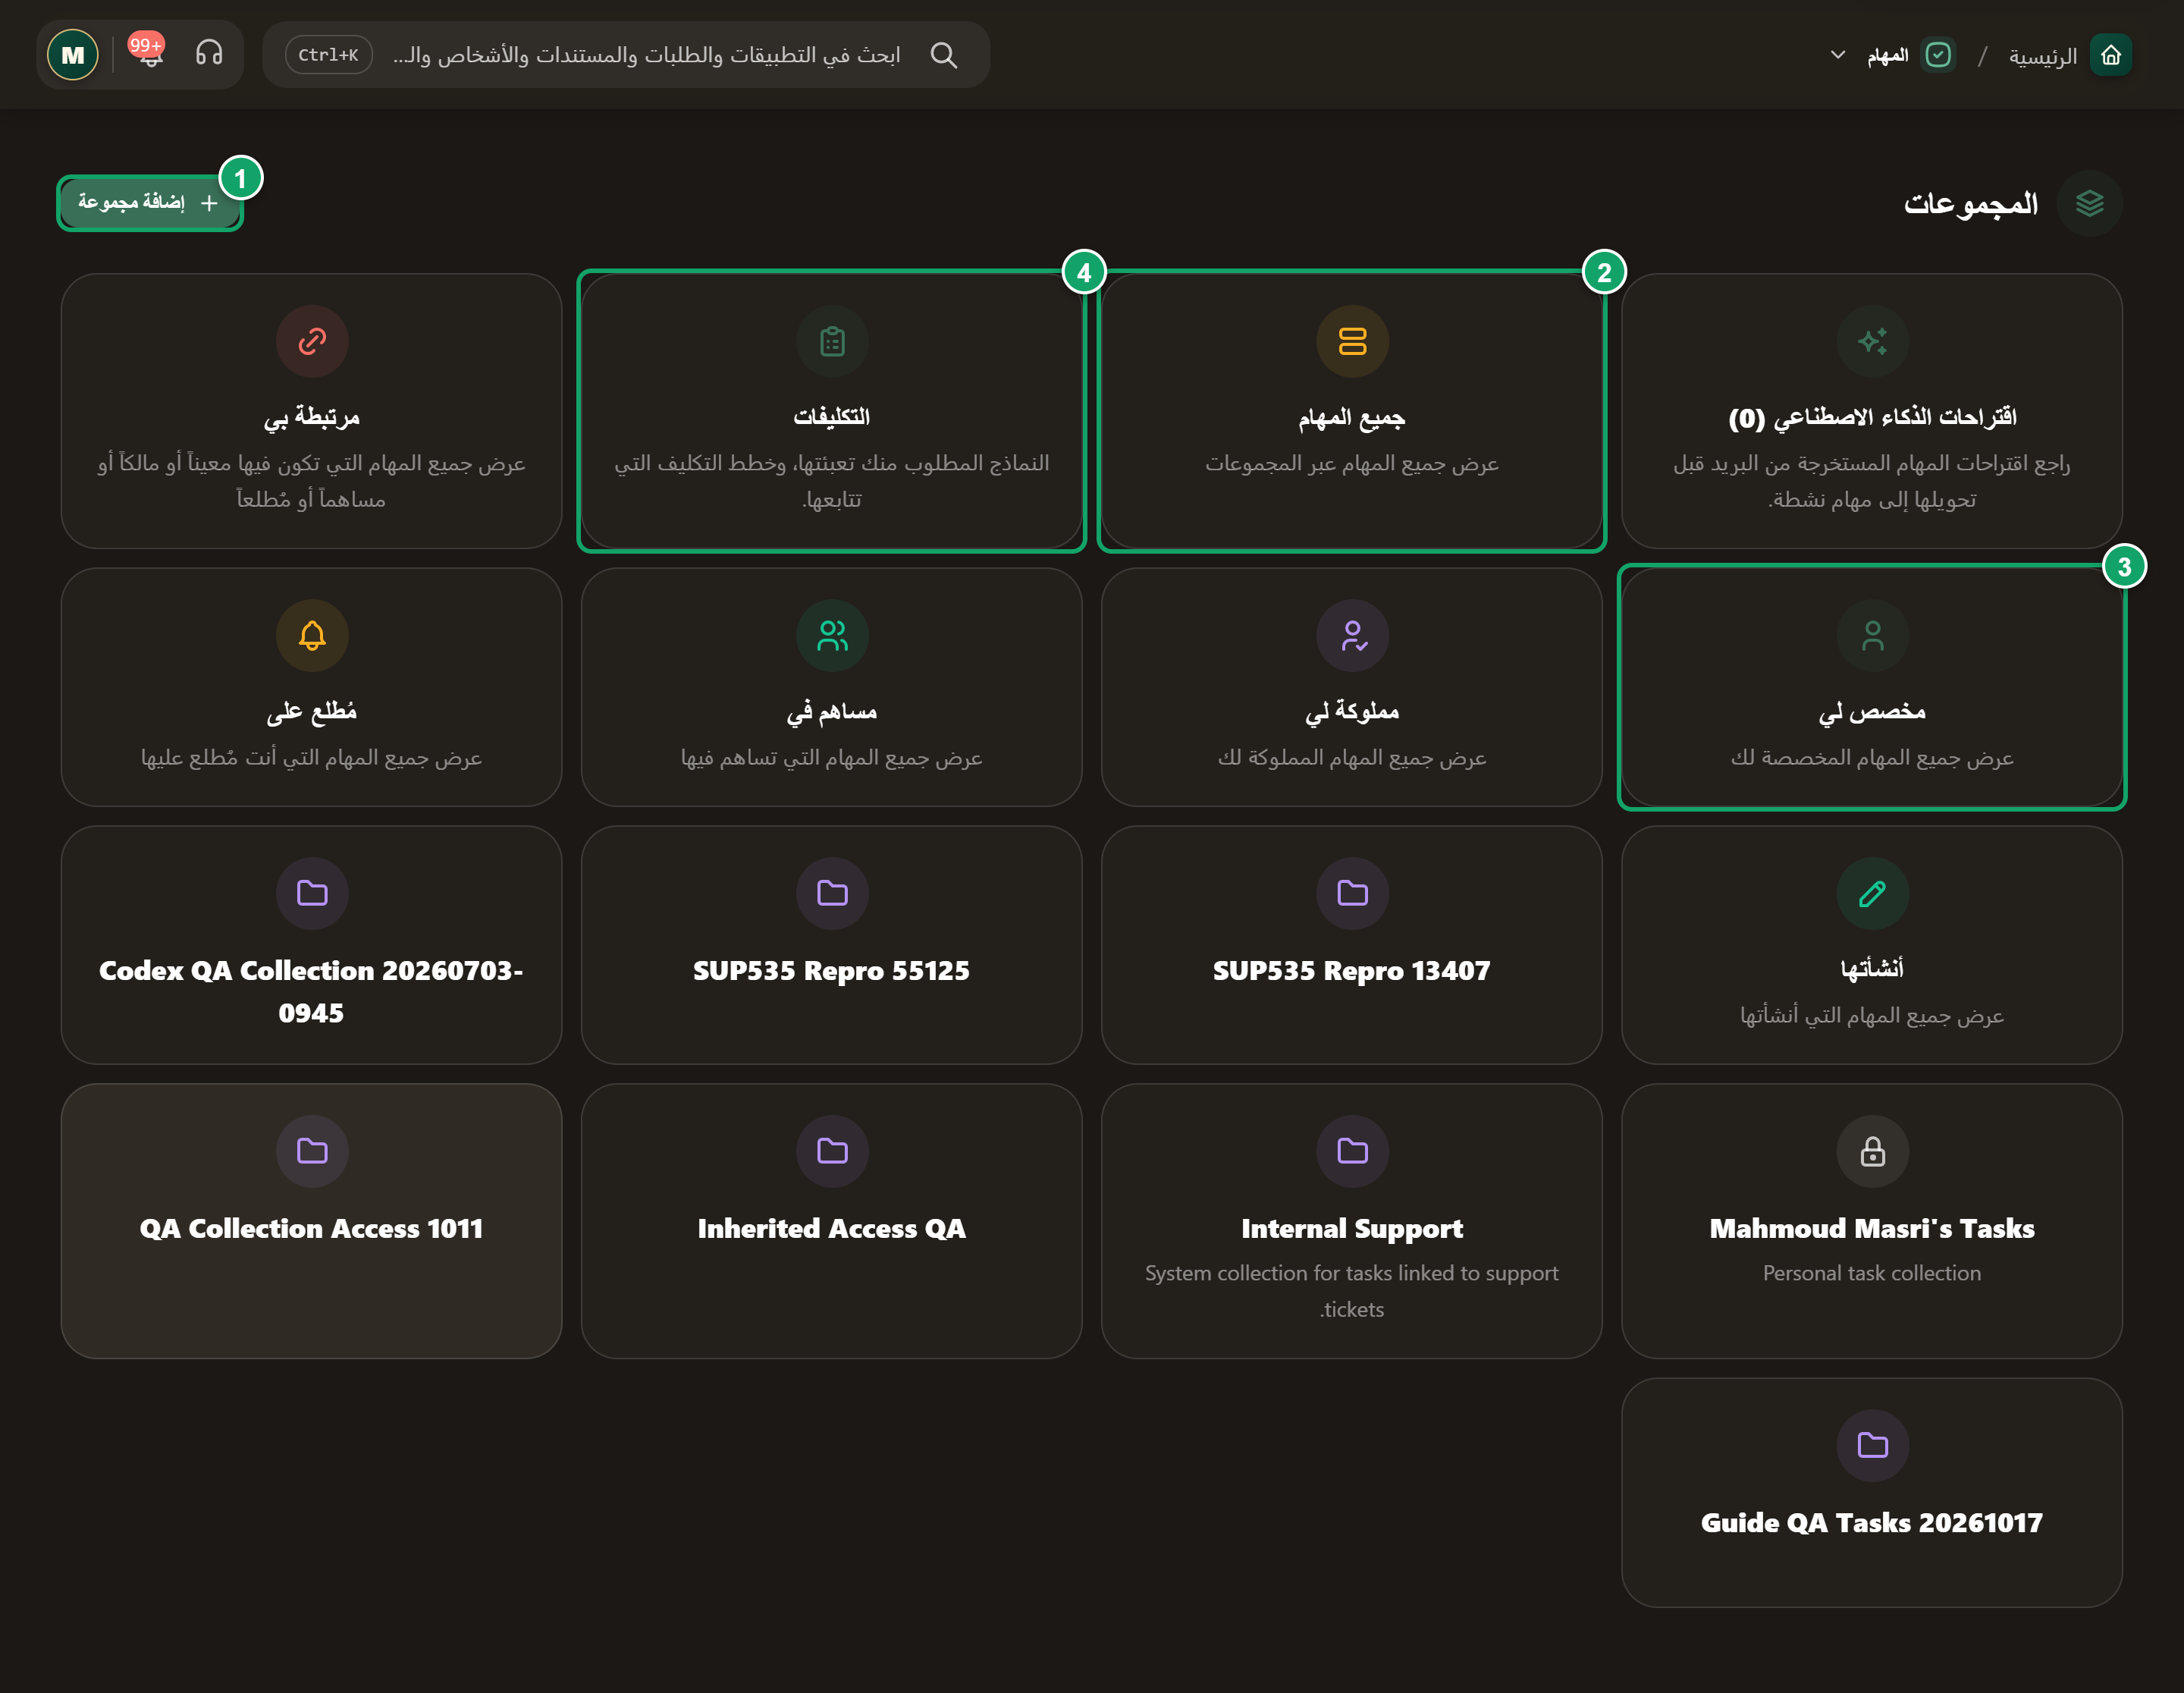
\includegraphics[width=0.95\linewidth,height=0.72\textheight,keepaspectratio]{figures/screens/ch04-collections-ar.png}
\caption{صفحة «المجموعات»: مدخل تطبيق المهام}
\label{fig:tasks-directory-screen}
\shotnote{تعرض صفحة «المجموعات» بطاقات جاهزة مثل «جميع المهام» و«مخصص لي» إلى جانب المجموعات التي أنشأتها المؤسسة، فتبدأ من البطاقة التي تخص عملك. أما «التكليفات» و«اقتراحات الذكاء الاصطناعي» فلكل منهما بطاقة مستقلة، ويشرح الدليل كلاً منهما في صفحة خاصة.}
\end{figure}

ابدأ بالمجموعات والعروض، ثم انتقل إلى إنشاء المهمة ومتابعتها وربطها بغيرها، واستخدم المهام الكبرى عندما تقسّم عملاً واسعاً. أما الاقتراحات والتكليفات فمساران متخصصان، والإعدادات من شأن المسؤول. وتشرح بعض الصفحات التالية تبويبات أو أدوات داخل المهمة، لا صفحات مستقلة في التطبيق.

\begin{table}[H]
\centering
\caption{من العمل اليومي إلى التهيئة}
\label{tab:tasks-pages-all}
\begin{tabularx}{\linewidth}{R{4.2cm} Y}
\rcHeaderRow
\thh{الصفحة} & \thh{ماذا تقدم هذه الصفحة؟}\\
المجموعات & تجمع المجموعة مهام العمل الواحد في مكان واحد.\\
عروض المهام & يغيّر العرض طريقة العثور على المهام ومتابعتها.\\
إنشاء المهمة وتفاصيلها & تسجّل المهمة النتيجة المطلوبة ومن يتولاها.\\
التقدم والنتائج والتواصل & تجمع المهمة ما أُنجز وما يعيق العمل وما يطلبه الزملاء بعضهم من بعض.\\
العلاقات والسجلات المرتبطة & تربط العلاقات المهمة بمصدر العمل أو بما يثبت إنجازه أو بمهمة أخرى.\\
المهام الكبرى & تجمع المهمة الكبرى عدة مهام تخدم نتيجة أوسع.\\
اقتراحات الذكاء الاصطناعي & الاقتراح عمل مستخرج من سياق البريد، ويحتاج إلى مراجعة قبل أن يصبح مهمة فعلية.\\
التكليفات & تعرض التكليفات النماذج المطلوب منك تعبئتها والعمل المرتبط بها.\\
إعدادات المهام & تحدّد إعدادات المهام أنواع العمل وتصنيفاته والعلاقات المتاحة.\\
قوالب الحالات & يحدّد قالب الحالة مراحل العمل والانتقالات بينها.\\
\end{tabularx}
\end{table}


\clearpage
\section{المجموعات}
\label{sec:tasks-feature-collections}

تجمع المجموعة مهام العمل المترابطة في مكان واحد. استخدم المجموعة المشتركة لعمل الفريق، والمجموعة الشخصية لتنظيم عملك الخاص.

\textbf{المسار ومن يستخدمه:} «المهام» ← «المجموعات». يستخدمها من ينظّم العمل ويوزّعه على الفريق.

\begin{rcnote}[مثال: شركة الأفق]
تخصص سارة مجموعة «زيارات الأفق» لمهام التحضير للزيارات، فيجد عمر فيها العمل المطلوب منه بدلاً من البحث في محادثات متفرقة.
\end{rcnote}

\begin{figure}[H]
\centering
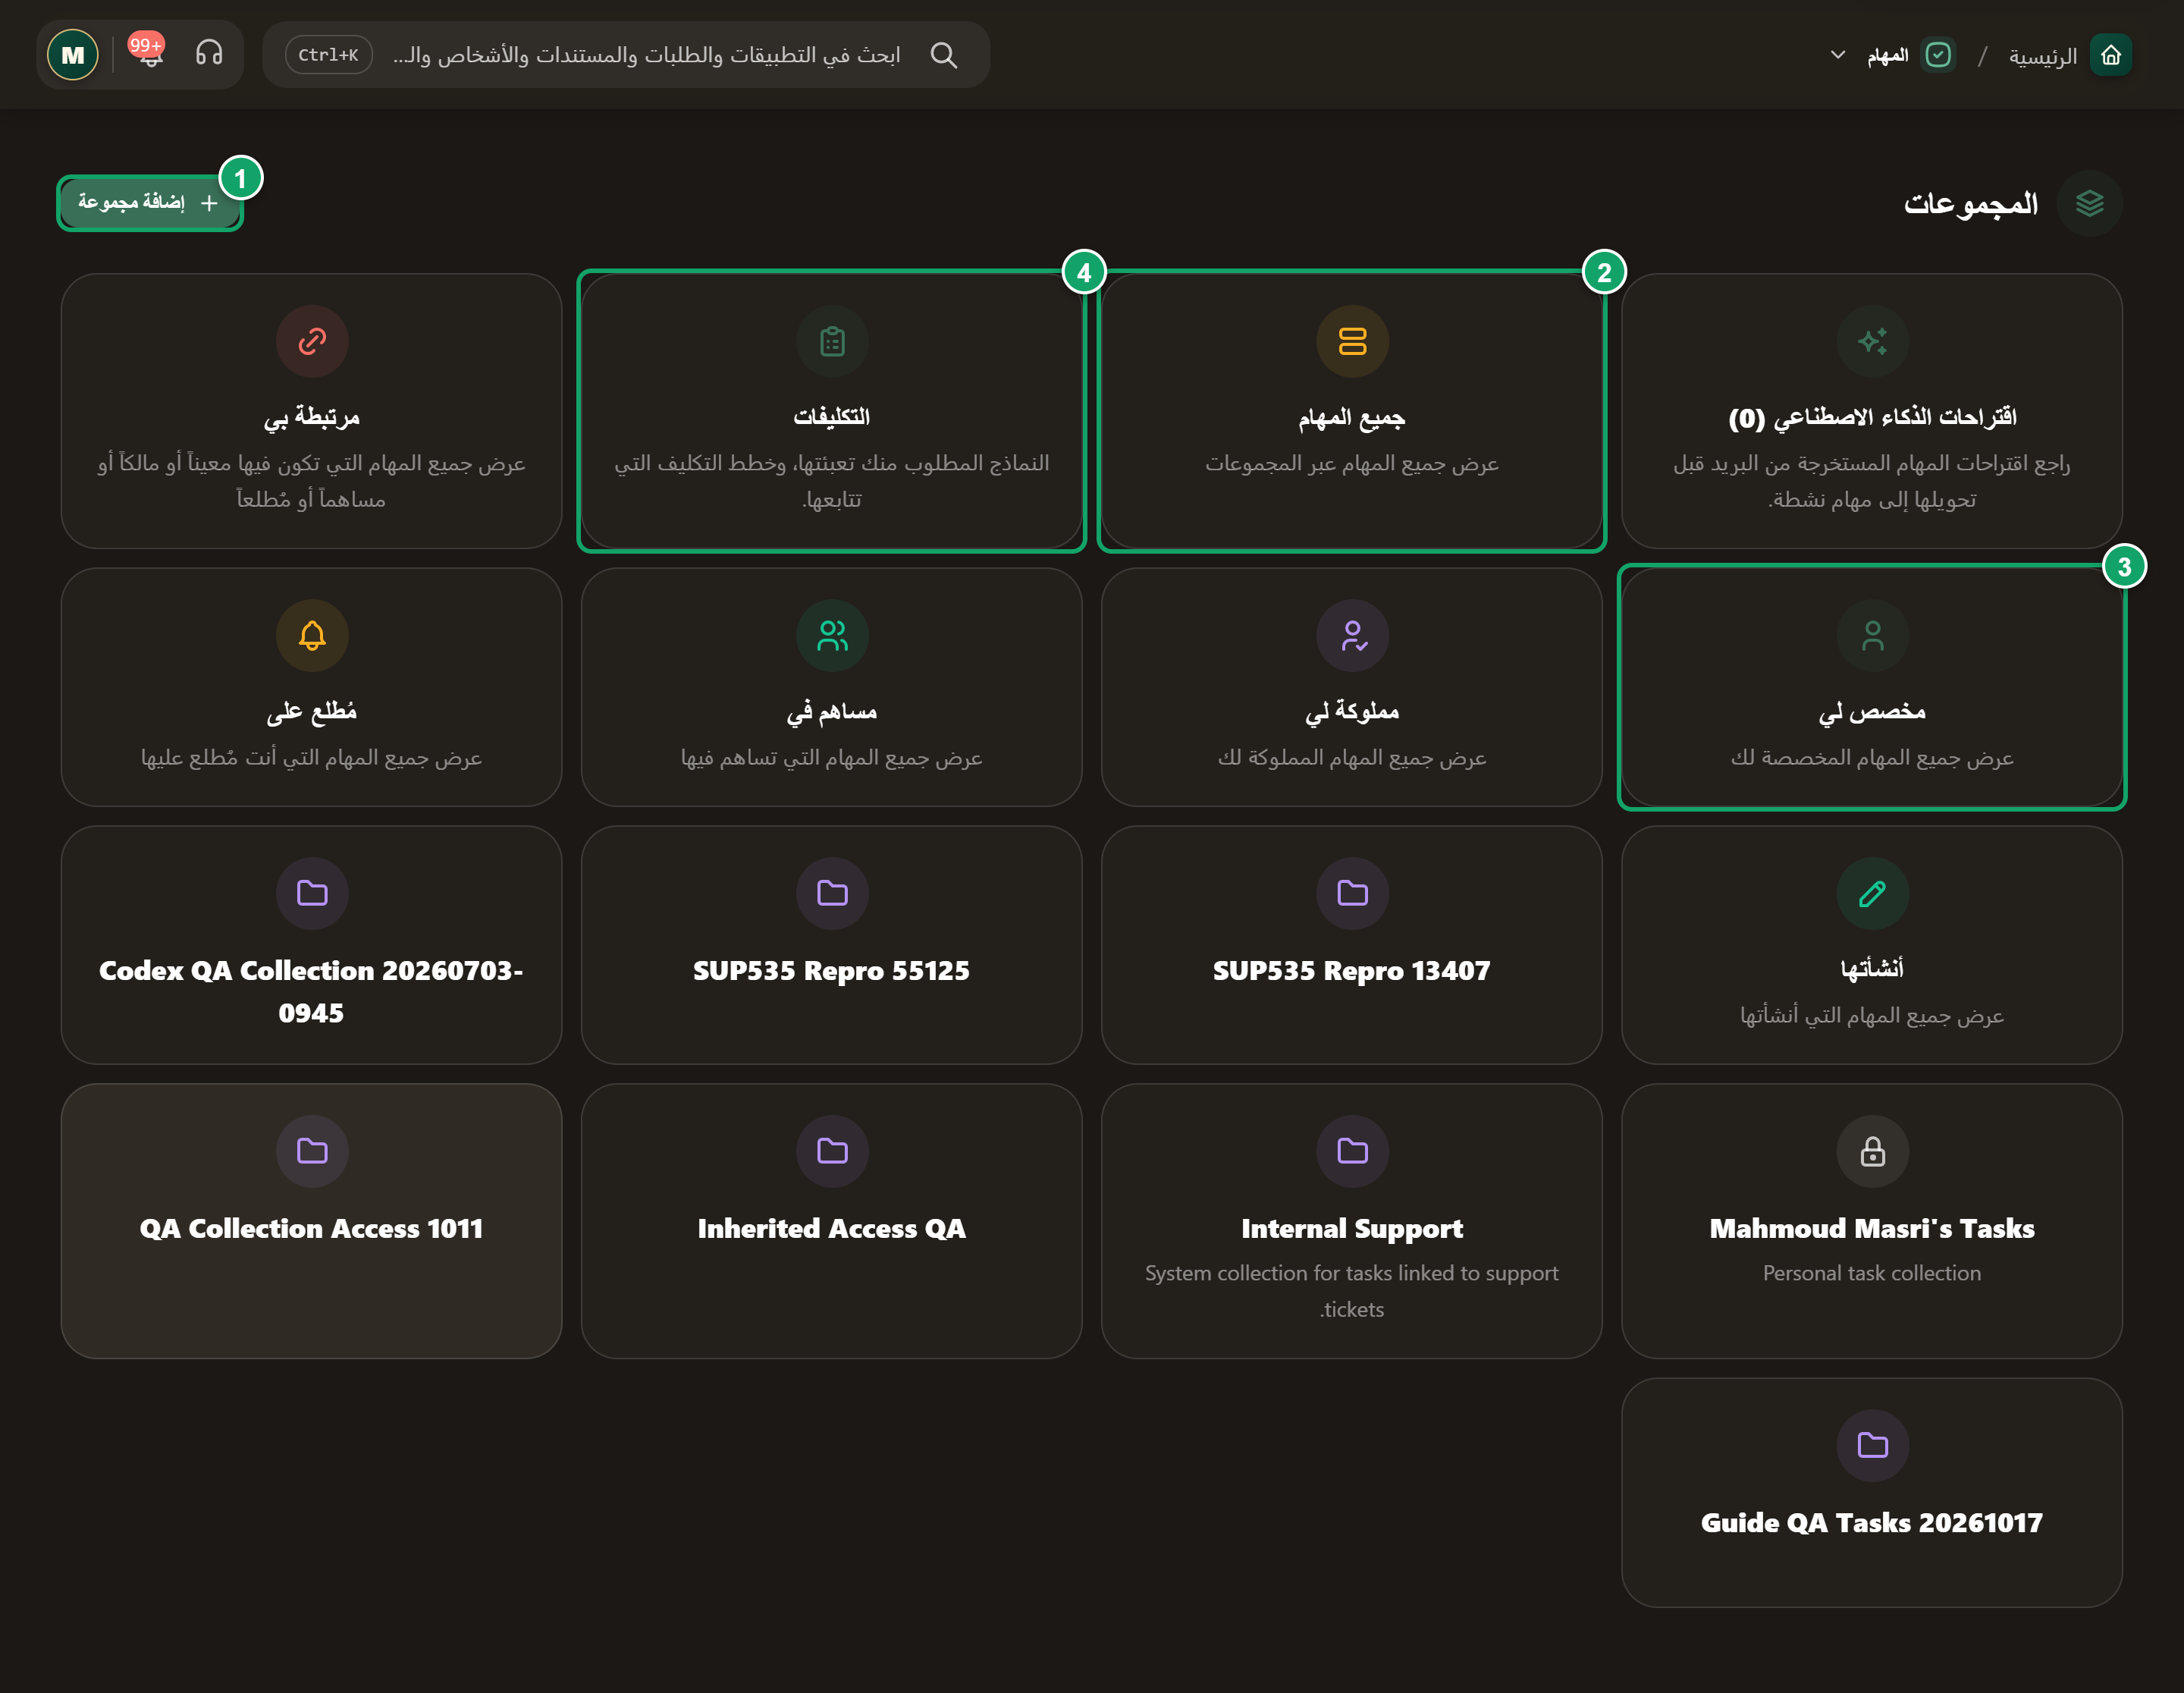
\includegraphics[width=0.95\linewidth,height=0.72\textheight,keepaspectratio]{figures/screens/ch04-collections-ar.png}
\caption{المجموعات والعروض المتاحة}
\label{fig:tasks-collections-collections}
\shotnote{تجمع صفحة «المجموعات» طريقين إلى العمل: بطاقات العروض الشخصية مثل «مخصص لي» و«التكليفات» و«اقتراحات الذكاء الاصطناعي»، ثم بطاقات المجموعات التي يمكنك الوصول إليها. لذلك ابدأ من العرض عندما تبحث عن عملك أنت، ومن المجموعة عندما تتابع عمل فريق بعينه. والمجموعات الظاهرة مجموعات اختبار في test2. ① «إضافة مجموعة». ② «جميع المهام»: يجمع كل ما يمكنك الوصول إليه. ③ «مخصص لي»: يعرض ما يجب أن تنفذه أنت. ④ «التكليفات»: تعرض النماذج المطلوب منك تعبئتها.}
\end{figure}

\begin{figure}[H]
\centering
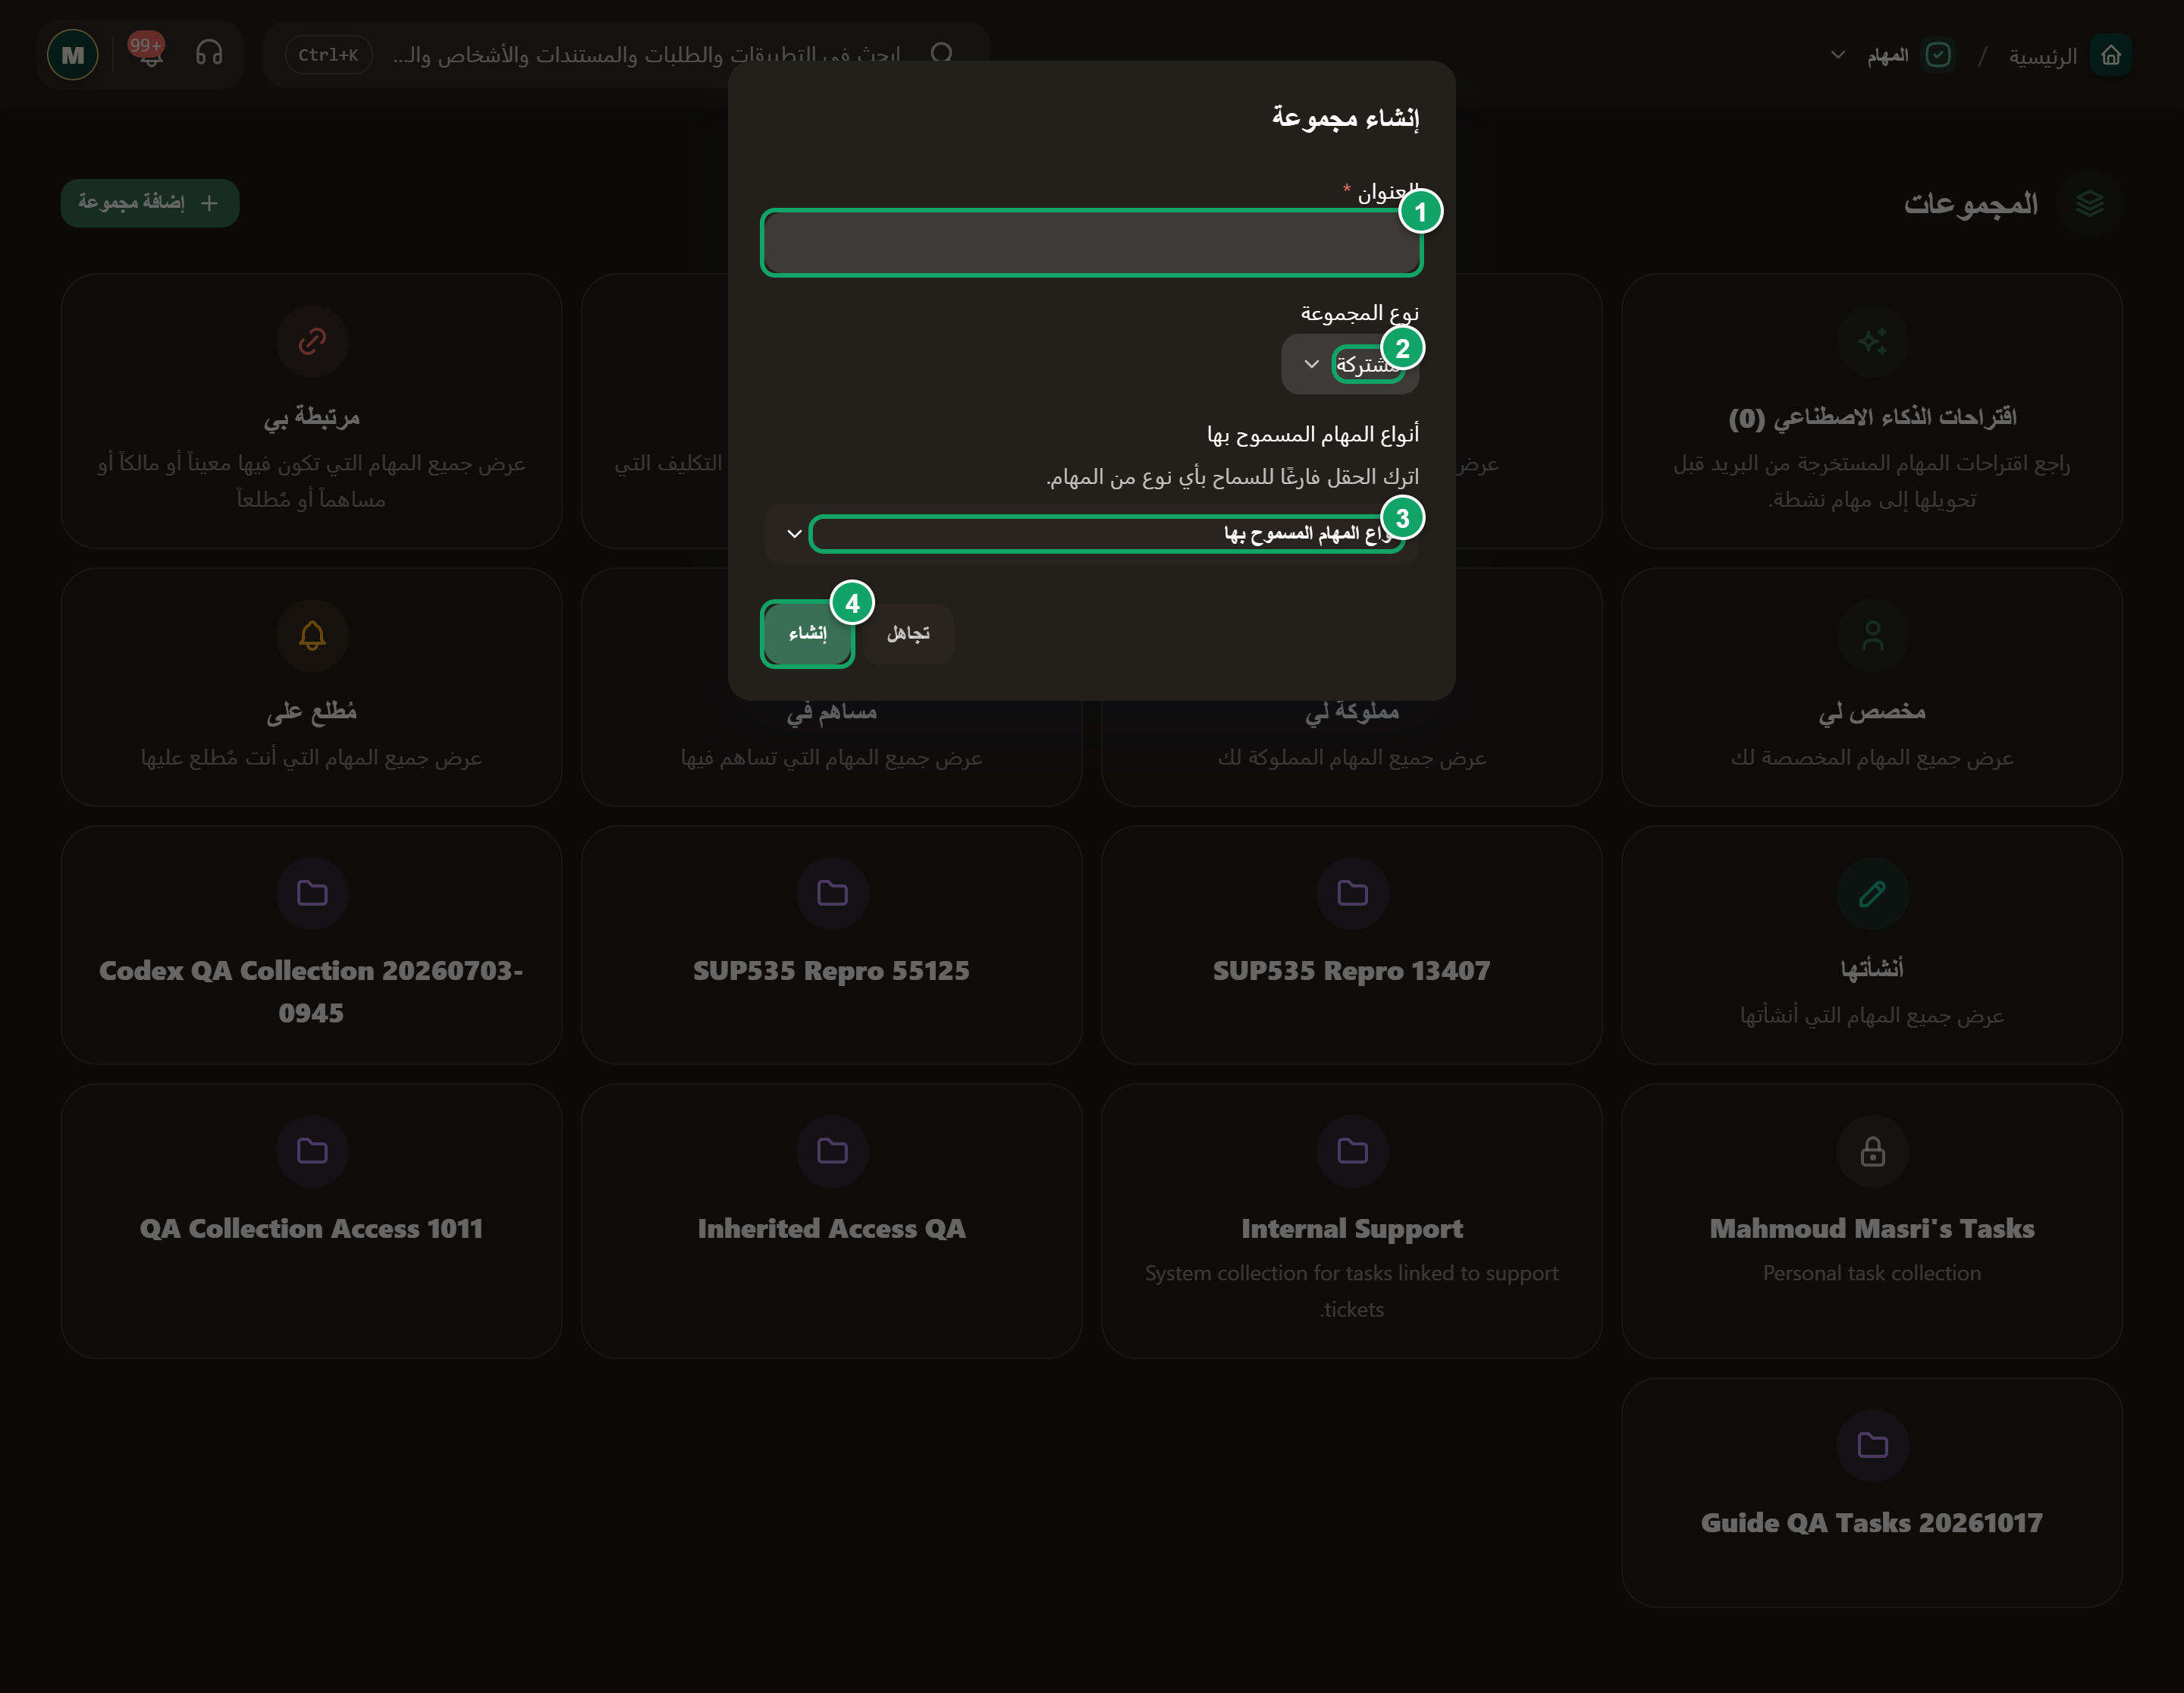
\includegraphics[width=0.95\linewidth,height=0.72\textheight,keepaspectratio]{figures/screens/ch04-collection-form-ar.png}
\caption{نموذج إنشاء مجموعة قبل الحفظ}
\label{fig:tasks-collections-collection-form}
\shotnote{يكفي لإنشاء المجموعة أن تكتب «العنوان» المطلوب وتختار «نوع المجموعة»، أي هل هي مشتركة أم شخصية. أما «أنواع المهام المسموح بها» فقيد اختياري: إذا تركته فارغاً قبلت المجموعة أي نوع متاح لك، وإذا حددت أنواعاً اقتصرت المهام فيها على تلك الأنواع. ① «العنوان» الإلزامي. ② «نوع المجموعة»: مشتركة أو شخصية. ③ «أنواع المهام المسموح بها»: قيد اختياري. ④ «إنشاء».}
\end{figure}

\begin{table}[H]
\centering
\caption{ما الذي تجده هنا؟}
\label{tab:tasks-collections-data}
\begin{tabularx}{\linewidth}{R{3.6cm} Y}
\rcHeaderRow
\thh{القسم} & \thh{المحتوى والإجراء}\\
العنوان والنوع & العنوان مطلوب، والنوع يميّز المجموعة الشخصية من المشتركة.\\
أنواع المهام المسموح بها & قيد اختياري يحدد الأنواع المقبولة داخل المجموعة، لكنه لا يمنحك صلاحية إنشاء نوع غير مسموح لك.\\
إعدادات المجموعة & تعديل البيانات والأنواع وإدارة المشاركة بحسب صلاحيتك. تأكد من وصول الفريق قبل الاعتماد على المجموعة.\\
\end{tabularx}
\end{table}

\begin{figure}[H]
\centering
\begin{tikzpicture}[node distance=0.5cm]
\node[stepBox] (a) {\RL{اختيار المجموعة}};
\node[stepBox,below=of a] (b) {\RL{مراجعة الوصول}};
\node[stepBox,below=of b] (c) {\RL{فتح مهام الفريق}};
\draw[flowsTo] (a) -- (b);
\draw[flowsTo] (b) -- (c);
\end{tikzpicture}
\rclegend
\caption{خطوات الاستخدام}
\label{fig:tasks-collections-flow}
\shotnote{يضع المخطط مراجعة الوصول بين اختيار المجموعة وتوزيع المهام فيها، لأن فتحك أنت للمجموعة لا يضمن أن الفريق يراها. فإذا وزّعت العمل في مجموعة لا يصل إليها المكلفون، لم يجدوا مهامهم فيها.}
\end{figure}

\subsection{خطوات العمل والتحقق}
\begin{enumerate}
\item ابحث أولاً عن المجموعة المطلوبة، فإن لم تجدها فاضغط «إضافة مجموعة».
\item اكتب عنواناً واضحاً، وحدد نوع المجموعة والأنواع المسموح بها عند الحاجة، ثم اضغط «إنشاء».
\item افتح المجموعة من بطاقتها، وقبل إسناد العمل تحقق من أن أعضاء الفريق المقصودين يستطيعون فتحها.
\end{enumerate}

\textbf{تحقق ومعالجة المشكلة:} يجب أن يظهر عنوان المجموعة عند فتحها. فإذا ظهرت رسالة «المجموعة غير متاحة»، فارجع إلى «المجموعات» وحدّث الصفحة، ثم اطلب مراجعة المشاركة والصلاحيات، ولا تنشئ نسخاً مكررة من المجموعة.

\clearpage
\section{عروض المهام}
\label{sec:tasks-feature-views}

يغيّر العرض طريقة العثور على المهام ومتابعتها دون أن يغيّر المهام نفسها. استخدم «قائمة» لمراجعة التفاصيل، و«لوحة» لتوزيع العمل حسب الحالة، و«المتابعة اليومية» لمراجعة تحديثات الفريق.

\textbf{المسار ومن يستخدمه:} «المهام» ← مجموعة أو أحد عروضك الشخصية. يستخدمها الموظف والمدير يومياً.

\begin{rcnote}[مثال: شركة الأفق]
يفتح عمر «مخصص لي» ليعرف العمل المطلوب منه، وتراجع سارة لوحة «زيارات الأفق» لترى المهام التي لم تبدأ بعد.
\end{rcnote}

\begin{figure}[H]
\centering
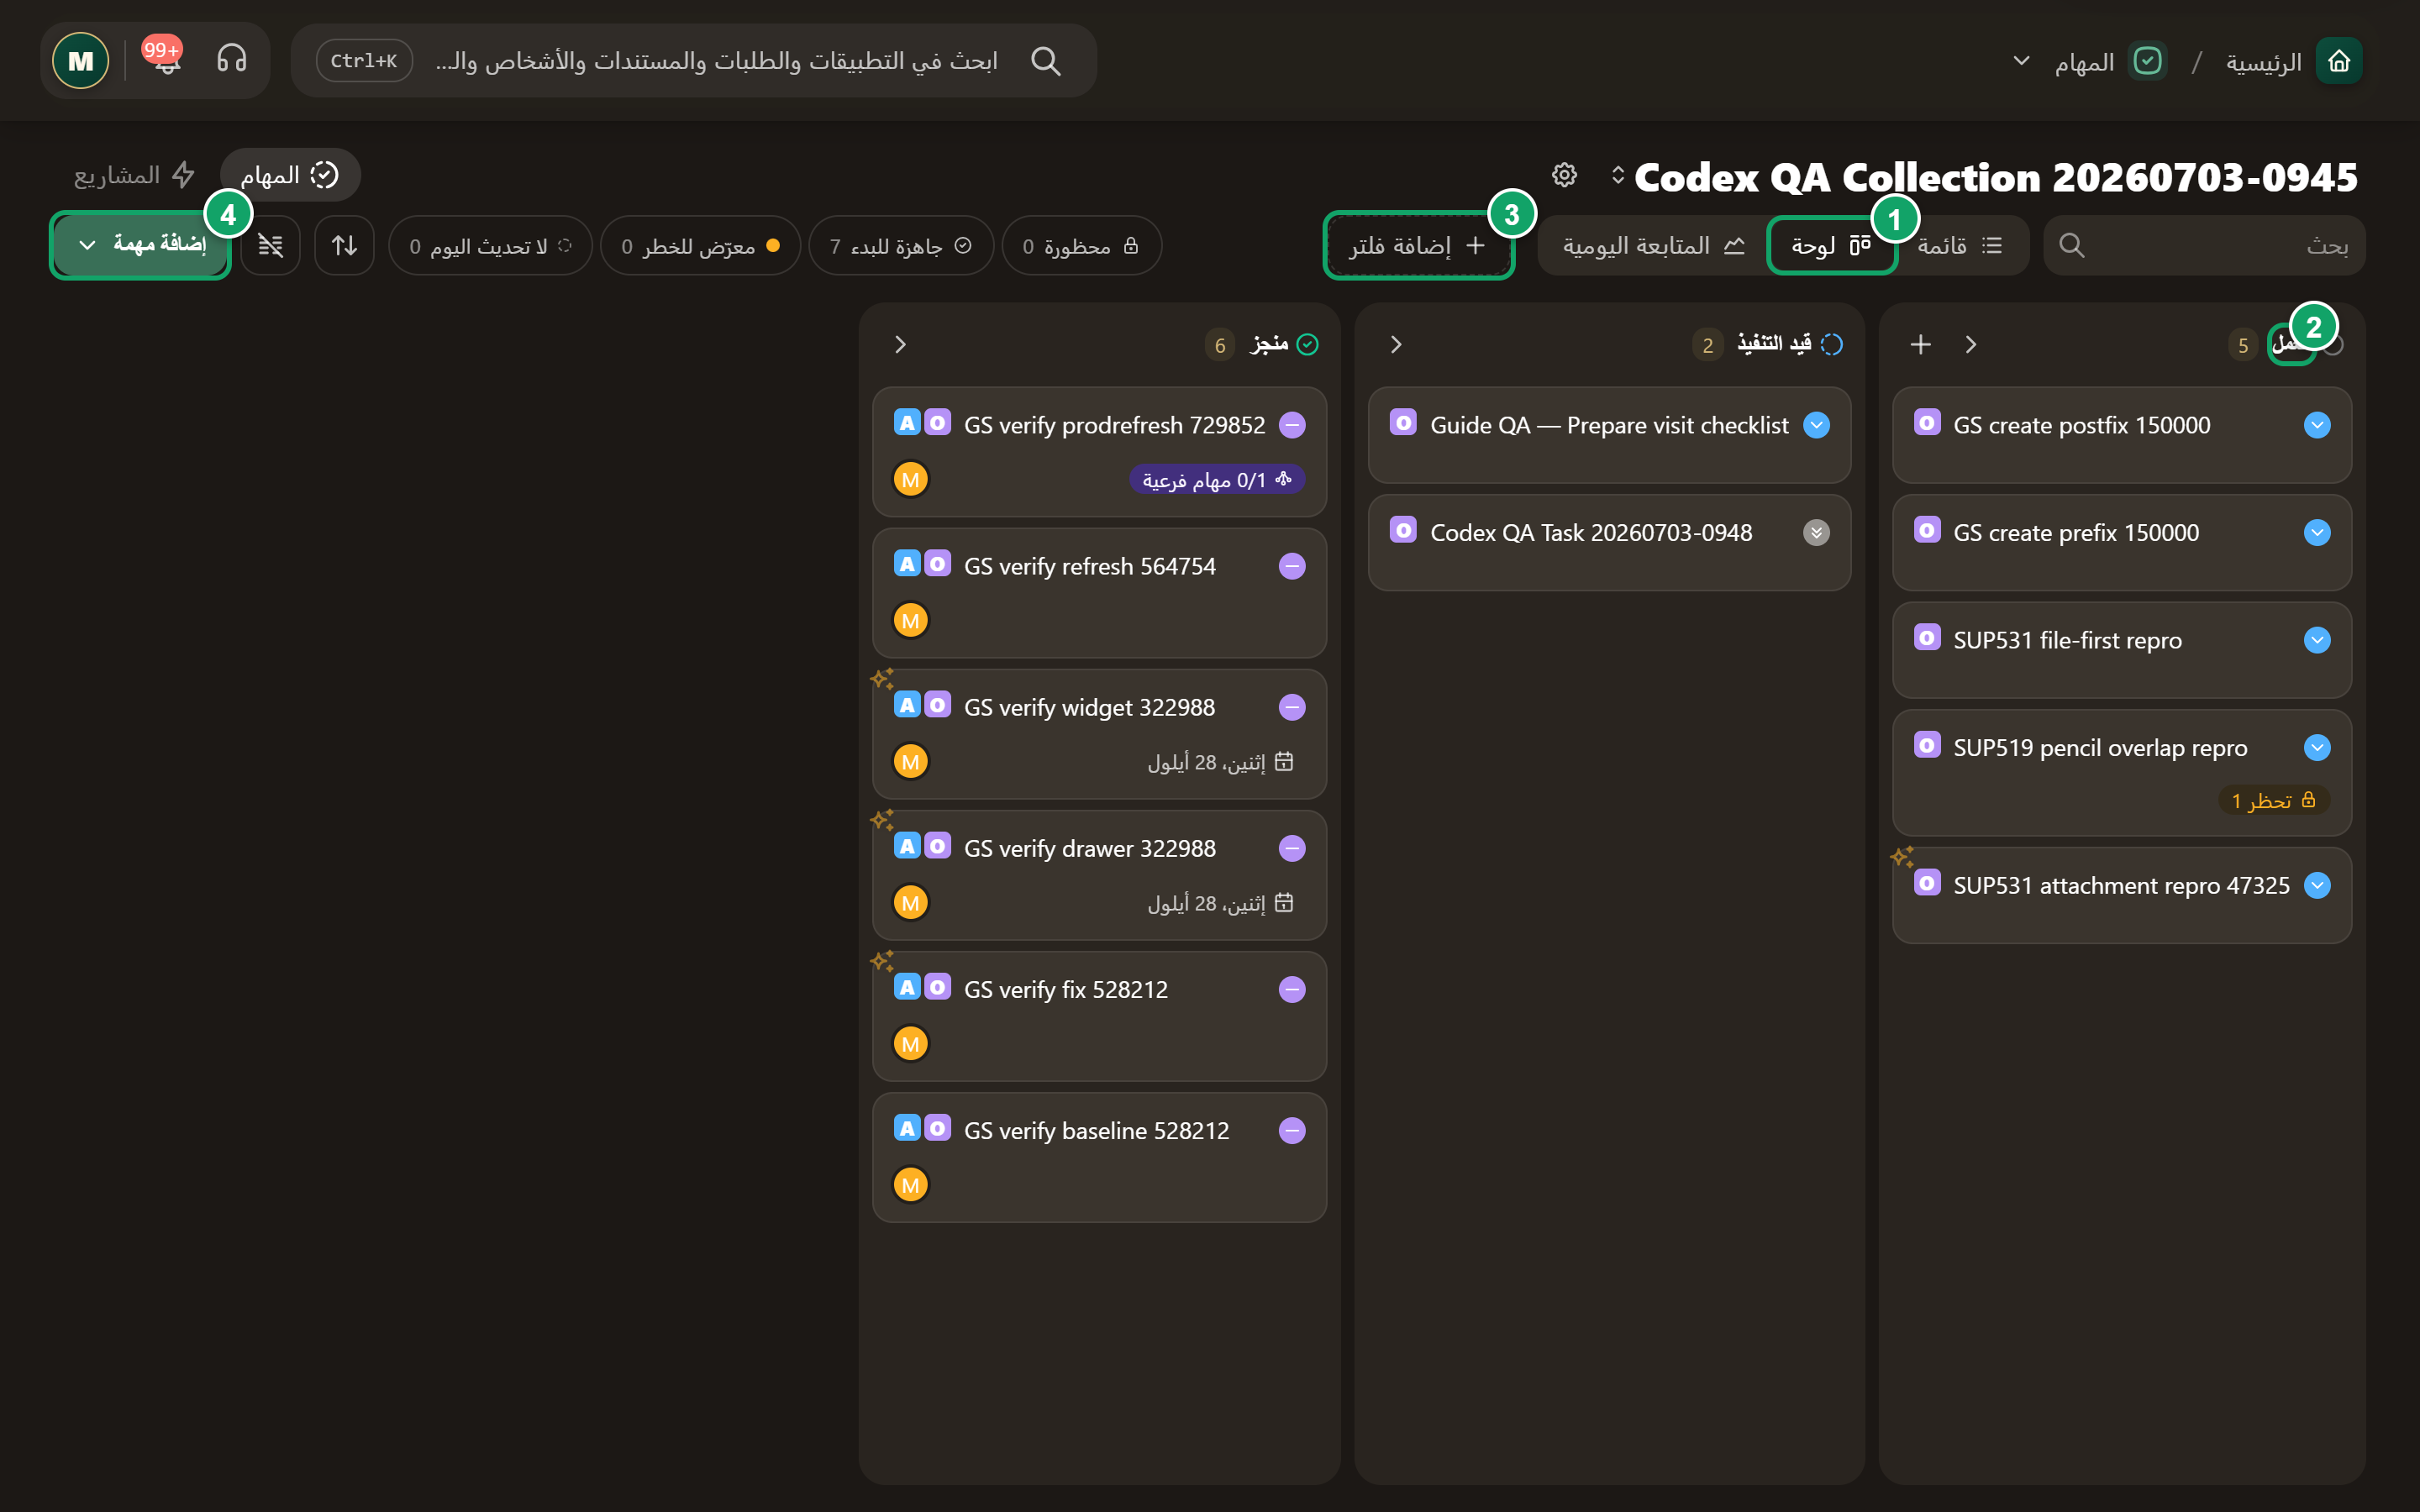
\includegraphics[width=0.95\linewidth,height=0.72\textheight,keepaspectratio]{figures/screens/ch04-board-ar.png}
\caption{لوحة مجموعة اختبار}
\label{fig:tasks-views-board}
\shotnote{تعرض «لوحة» مهام المجموعة في أعمدة تمثل الحالات، مثل «للعمل» و«قيد التنفيذ» و«منجز»، فترى في نظرة واحدة أين يقف العمل وأين يتراكم. وتعرض الشارات مثل «محظورة» و«جاهزة للبدء» عدد المهام التي تحتاج انتباهك. ولا تعني رؤيتك للمهمة أنك تستطيع تعديلها أو نقلها. ① «لوحة». ② عمود «للعمل» وفيه المهام التي لم تبدأ. ③ «إضافة فلتر». ④ «إضافة مهمة».}
\end{figure}

\begin{figure}[H]
\centering
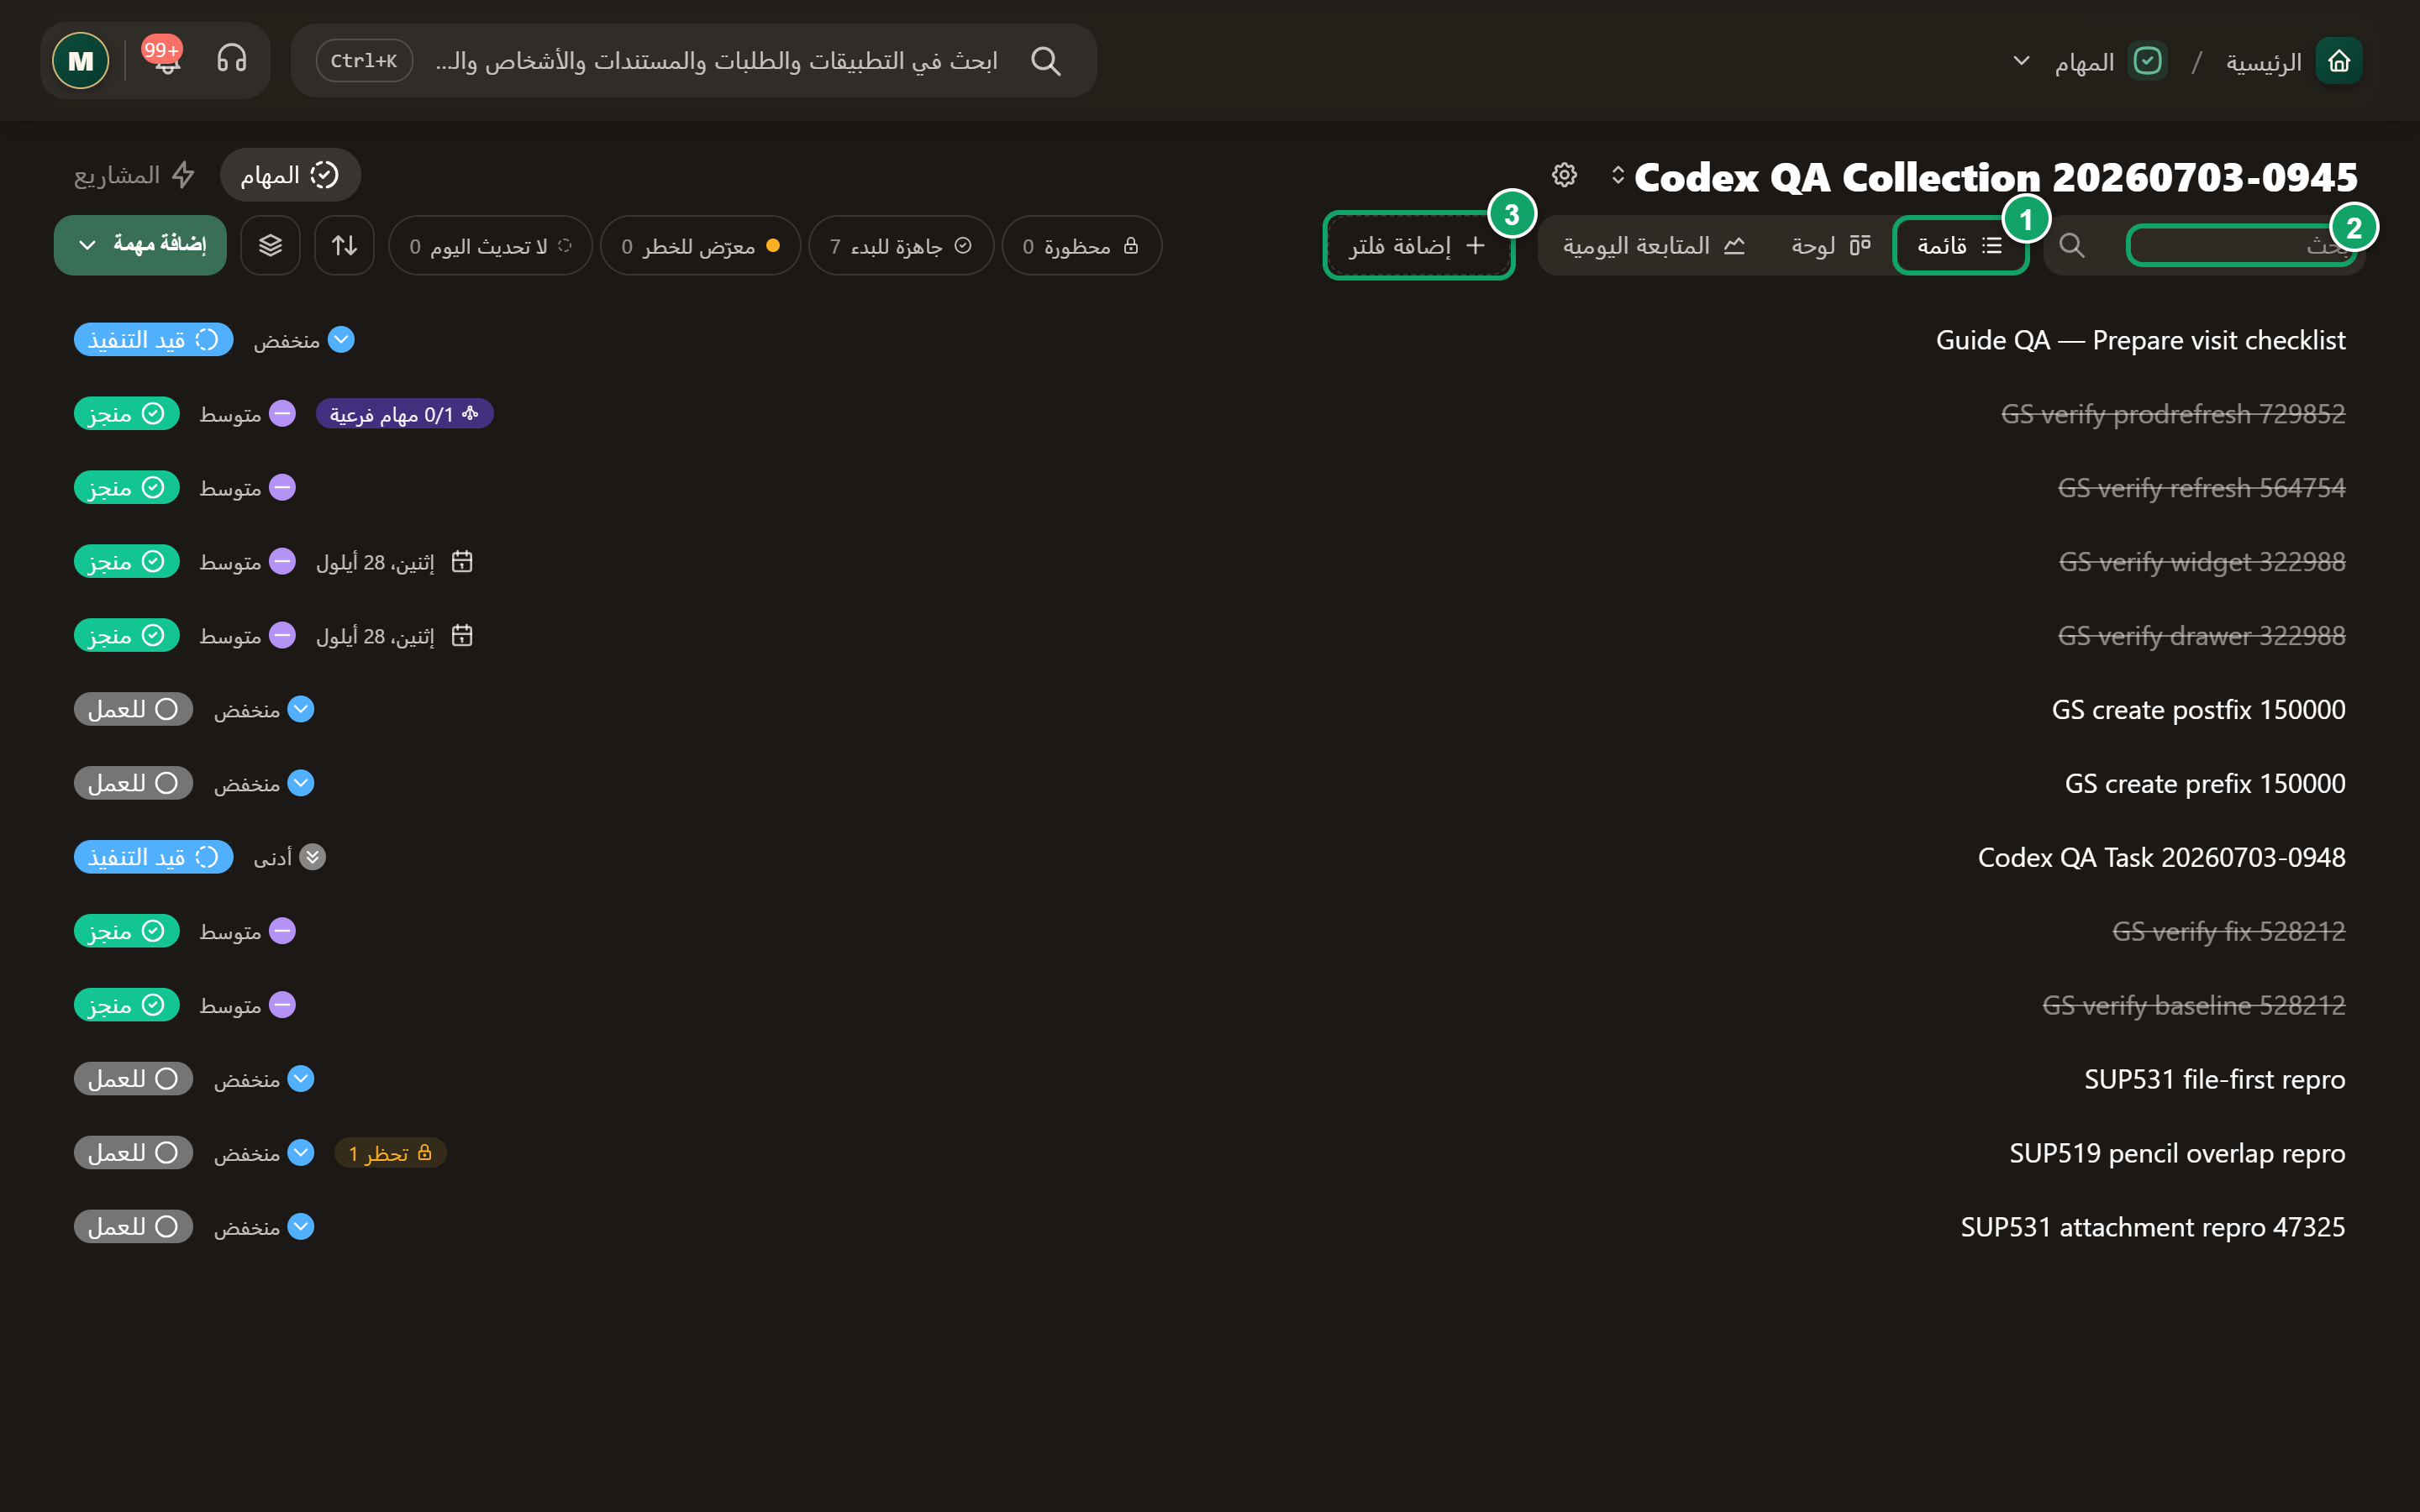
\includegraphics[width=0.95\linewidth,height=0.72\textheight,keepaspectratio]{figures/screens/ch04-list-ar.png}
\caption{عرض القائمة}
\label{fig:tasks-views-list}
\shotnote{يعرض «قائمة» المهام نفسها في صفوف تبيّن حالة كل مهمة وأولويتها وموعدها، وتظهر المهام المنجزة بخط مشطوب. لذلك يناسب هذا العرض مقارنة المهام ومراجعة تفاصيلها، ويساعدك البحث و«إضافة فلتر» والترتيب على تضييق النتائج عندما تكثر المهام. ① «قائمة». ② مربع «بحث» للعثور على المهمة بعنوانها. ③ «إضافة فلتر».}
\end{figure}

\begin{figure}[H]
\centering
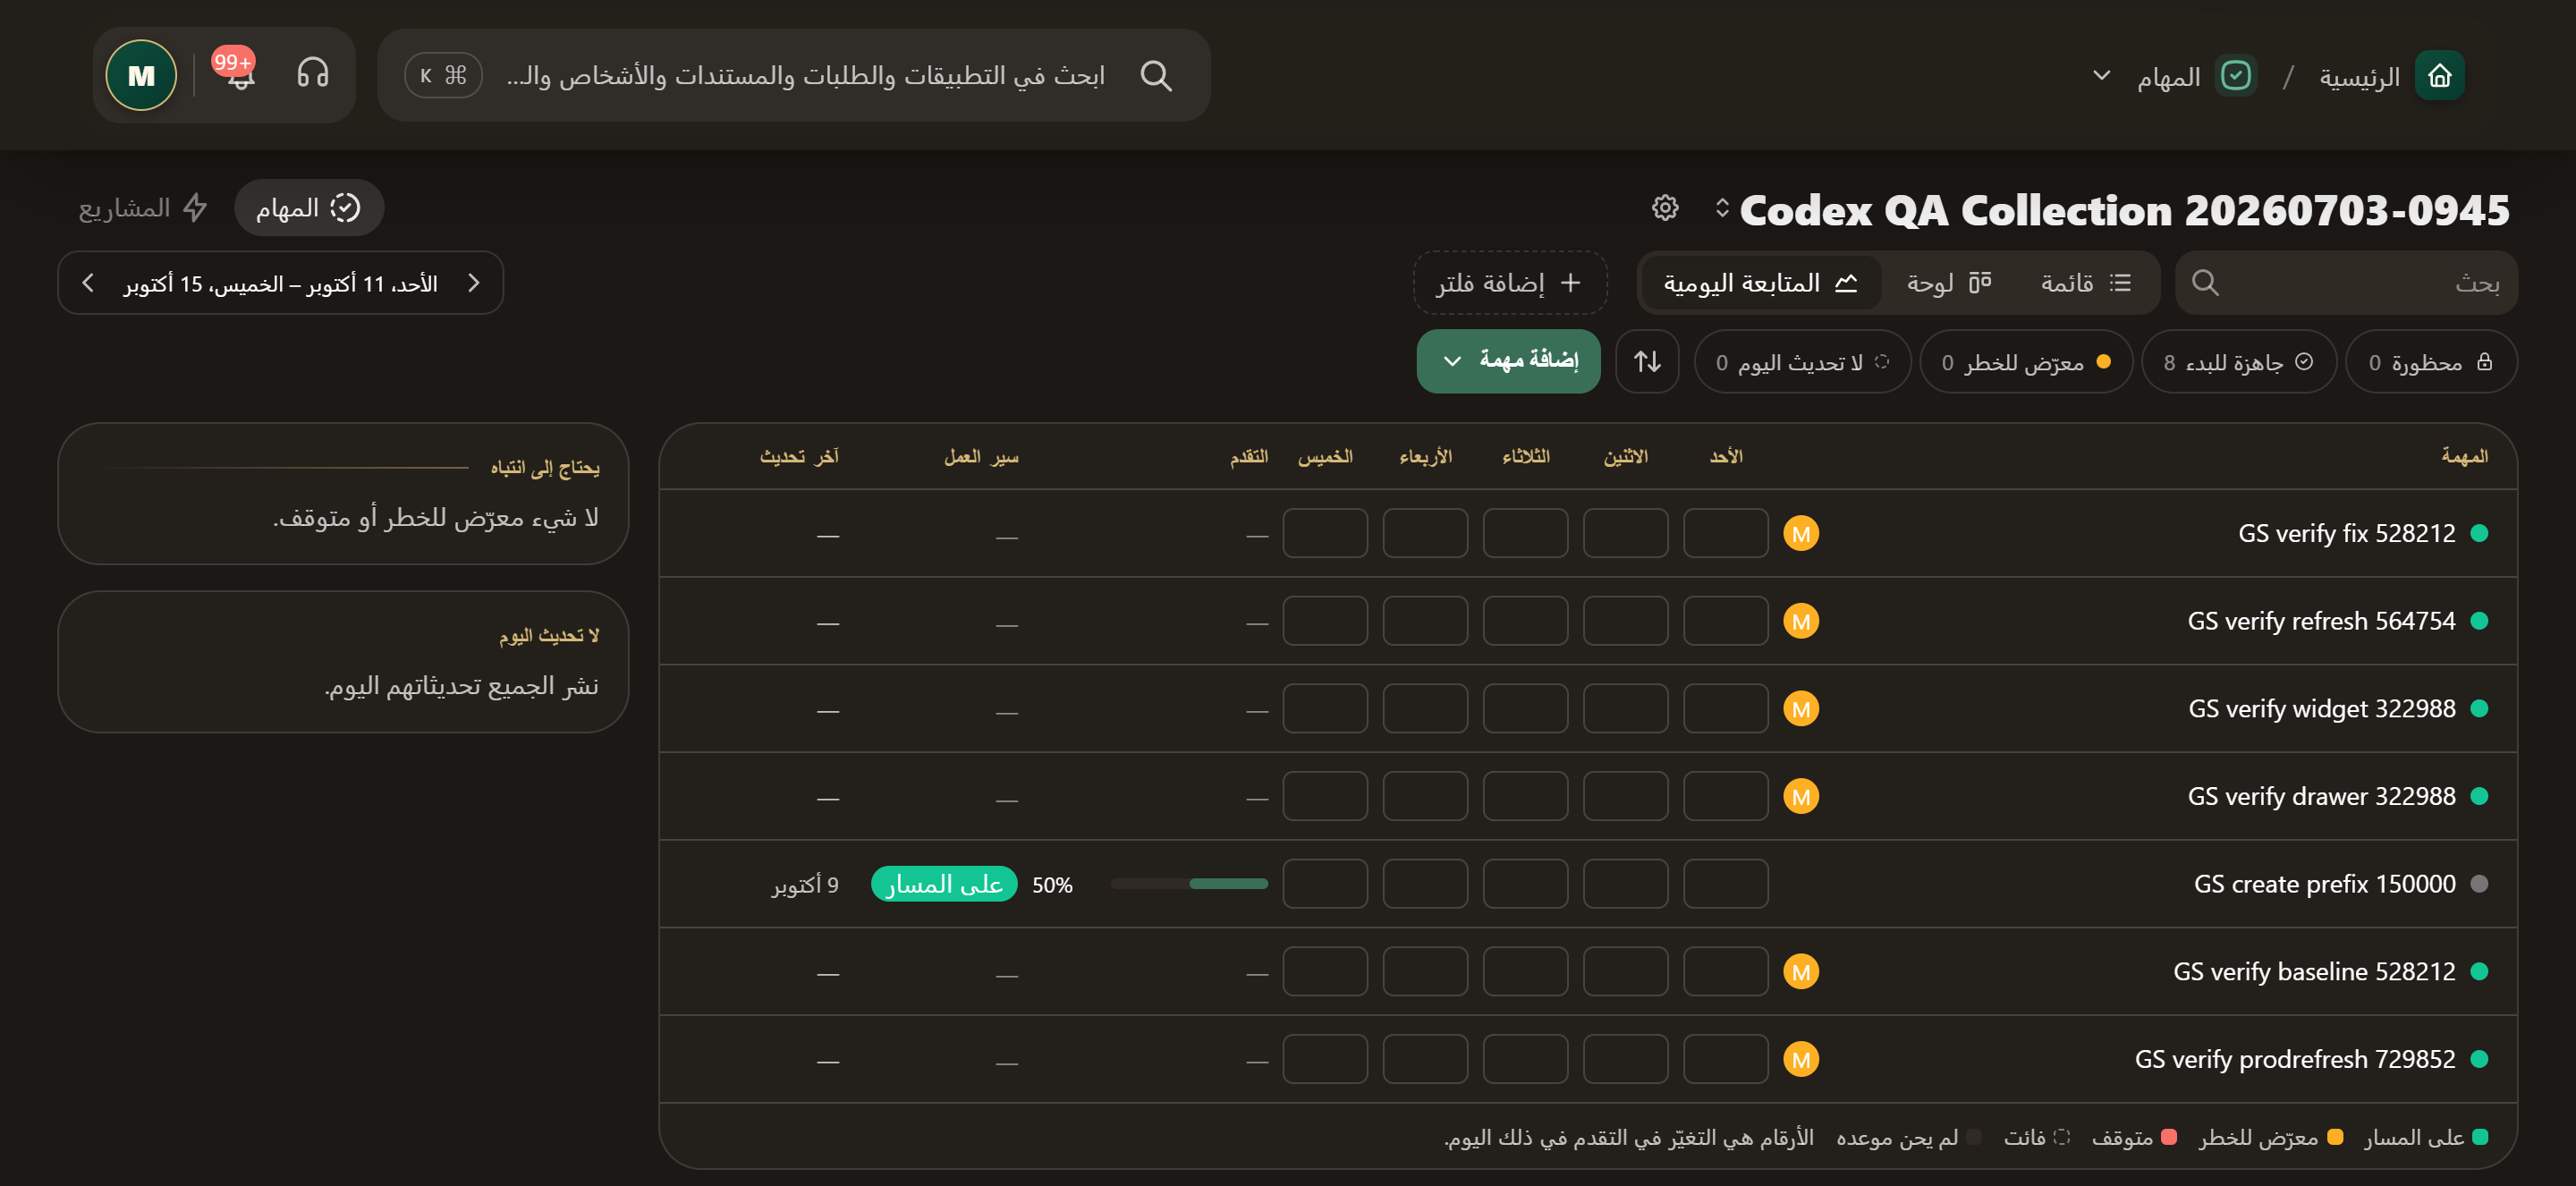
\includegraphics[width=0.95\linewidth,height=0.72\textheight,keepaspectratio]{figures/screens/ch04-checkins-ar.png}
\caption{عرض المتابعة اليومية}
\label{fig:tasks-views-checkins}
\shotnote{يعرض «المتابعة اليومية» تحديثات كل مهمة على أيام الأسبوع المحدد، مع التقدم و«سير العمل» و«آخر تحديث». وتجمع بطاقتا «يحتاج إلى انتباه» و«لا تحديث اليوم» ما يستدعي المتابعة. ولا يعني غياب التحديث أن المهمة اكتملت، بل أن أحداً لم ينشر عنها تحديثاً. ① «المتابعة اليومية». ② «يحتاج إلى انتباه»: المهام المعرضة للخطر أو المحظورة. ③ «لا تحديث اليوم».}
\end{figure}

\begin{table}[H]
\centering
\caption{ما الذي تجده هنا؟}
\label{tab:tasks-views-data}
\begin{tabularx}{\linewidth}{R{3.6cm} Y}
\rcHeaderRow
\thh{القسم} & \thh{المحتوى والإجراء}\\
جميع المهام؛ مرتبطة بي & الأول يجمع كل ما يمكنك الوصول إليه، والثاني يقتصر على المهام التي لك فيها دور.\\
مخصص لي؛ مملوكة لي & الأول يعرض التنفيذ المطلوب منك، والثاني يعرض المهام التي تتحمل مسؤولية نتيجتها.\\
مساهم في؛ مُطلع على؛ أنشأتها & عروض منفصلة للمهام التي تساهم فيها، والتي تتابعها للاطلاع، والتي أنشأتها.\\
البحث والتصفية والعرض & ابحث بالعنوان، ثم صفِّ النتائج ورتّبها وجمّعها بالخيارات المعروضة. أما إجراءات اللوحة الجماعية فتخضع لصلاحيات المهام وانتقالات حالاتها.\\
\end{tabularx}
\end{table}

\begin{figure}[H]
\centering
\begin{tikzpicture}[node distance=0.5cm]
\node[stepBox] (a) {\RL{اختيار دور أو مجموعة}};
\node[stepBox,below=of a] (b) {\RL{بحث وتصفية}};
\node[stepBox,below=of b] (c) {\RL{فتح المهمة}};
\draw[flowsTo] (a) -- (b);
\draw[flowsTo] (b) -- (c);
\end{tikzpicture}
\rclegend
\caption{خطوات الاستخدام}
\label{fig:tasks-views-flow}
\shotnote{يبيّن المخطط ترتيب البحث: ابدأ بالعرض الذي يطابق دورك أو بالمجموعة التي تتابعها، ثم ضيّق النتائج، وبعدها افتح المهمة. فإذا بدأت من عرض لا يخصك، فقد تظن أن المهمة مفقودة وهي في عرض آخر.}
\end{figure}

\subsection{خطوات العمل والتحقق}
\begin{enumerate}
\item افتح المجموعة أو العرض المناسب لدورك، ثم ابحث عن عنوان المهمة.
\item انتقل بين «قائمة» و«لوحة»، وراجع التصفية قبل أن تستنتج أن المهمة مفقودة.
\item افتح المهمة من بطاقتها، وإذا ظهرت قائمة إجراءات فاختر «فتح». ثم راجع حالتها والمسؤول عنها.
\end{enumerate}

\textbf{تحقق ومعالجة المشكلة:} إذا لم تجد المهمة، فأزل التصفية وراجع المجموعة ودورك وصلاحية الوصول. وتذكّر أن تغيير العرض لا يغيّر حالة العمل.

\clearpage
\section{إنشاء المهمة وتفاصيلها}
\label{sec:tasks-feature-details}

تسجّل المهمة نتيجة مطلوبة ومن يتولاها. اكتب عنواناً محدداً، ثم حدد المسؤولية والموعد والمعلومات اللازمة للتنفيذ.

\textbf{المسار ومن يستخدمه:} «المهام» ← مجموعة ← «إضافة مهمة». يستخدمها من يوزّع العمل ومن ينفّذه.

\begin{rcnote}[مثال: شركة الأفق]
تنشئ سارة مهمة «تجهيز قائمة الزيارة» في مجموعة «زيارات الأفق» وتسندها إلى عمر قبل موعد الزيارة، بينما تبقى هي المسؤولة عن النتيجة.
\end{rcnote}

\begin{figure}[H]
\centering
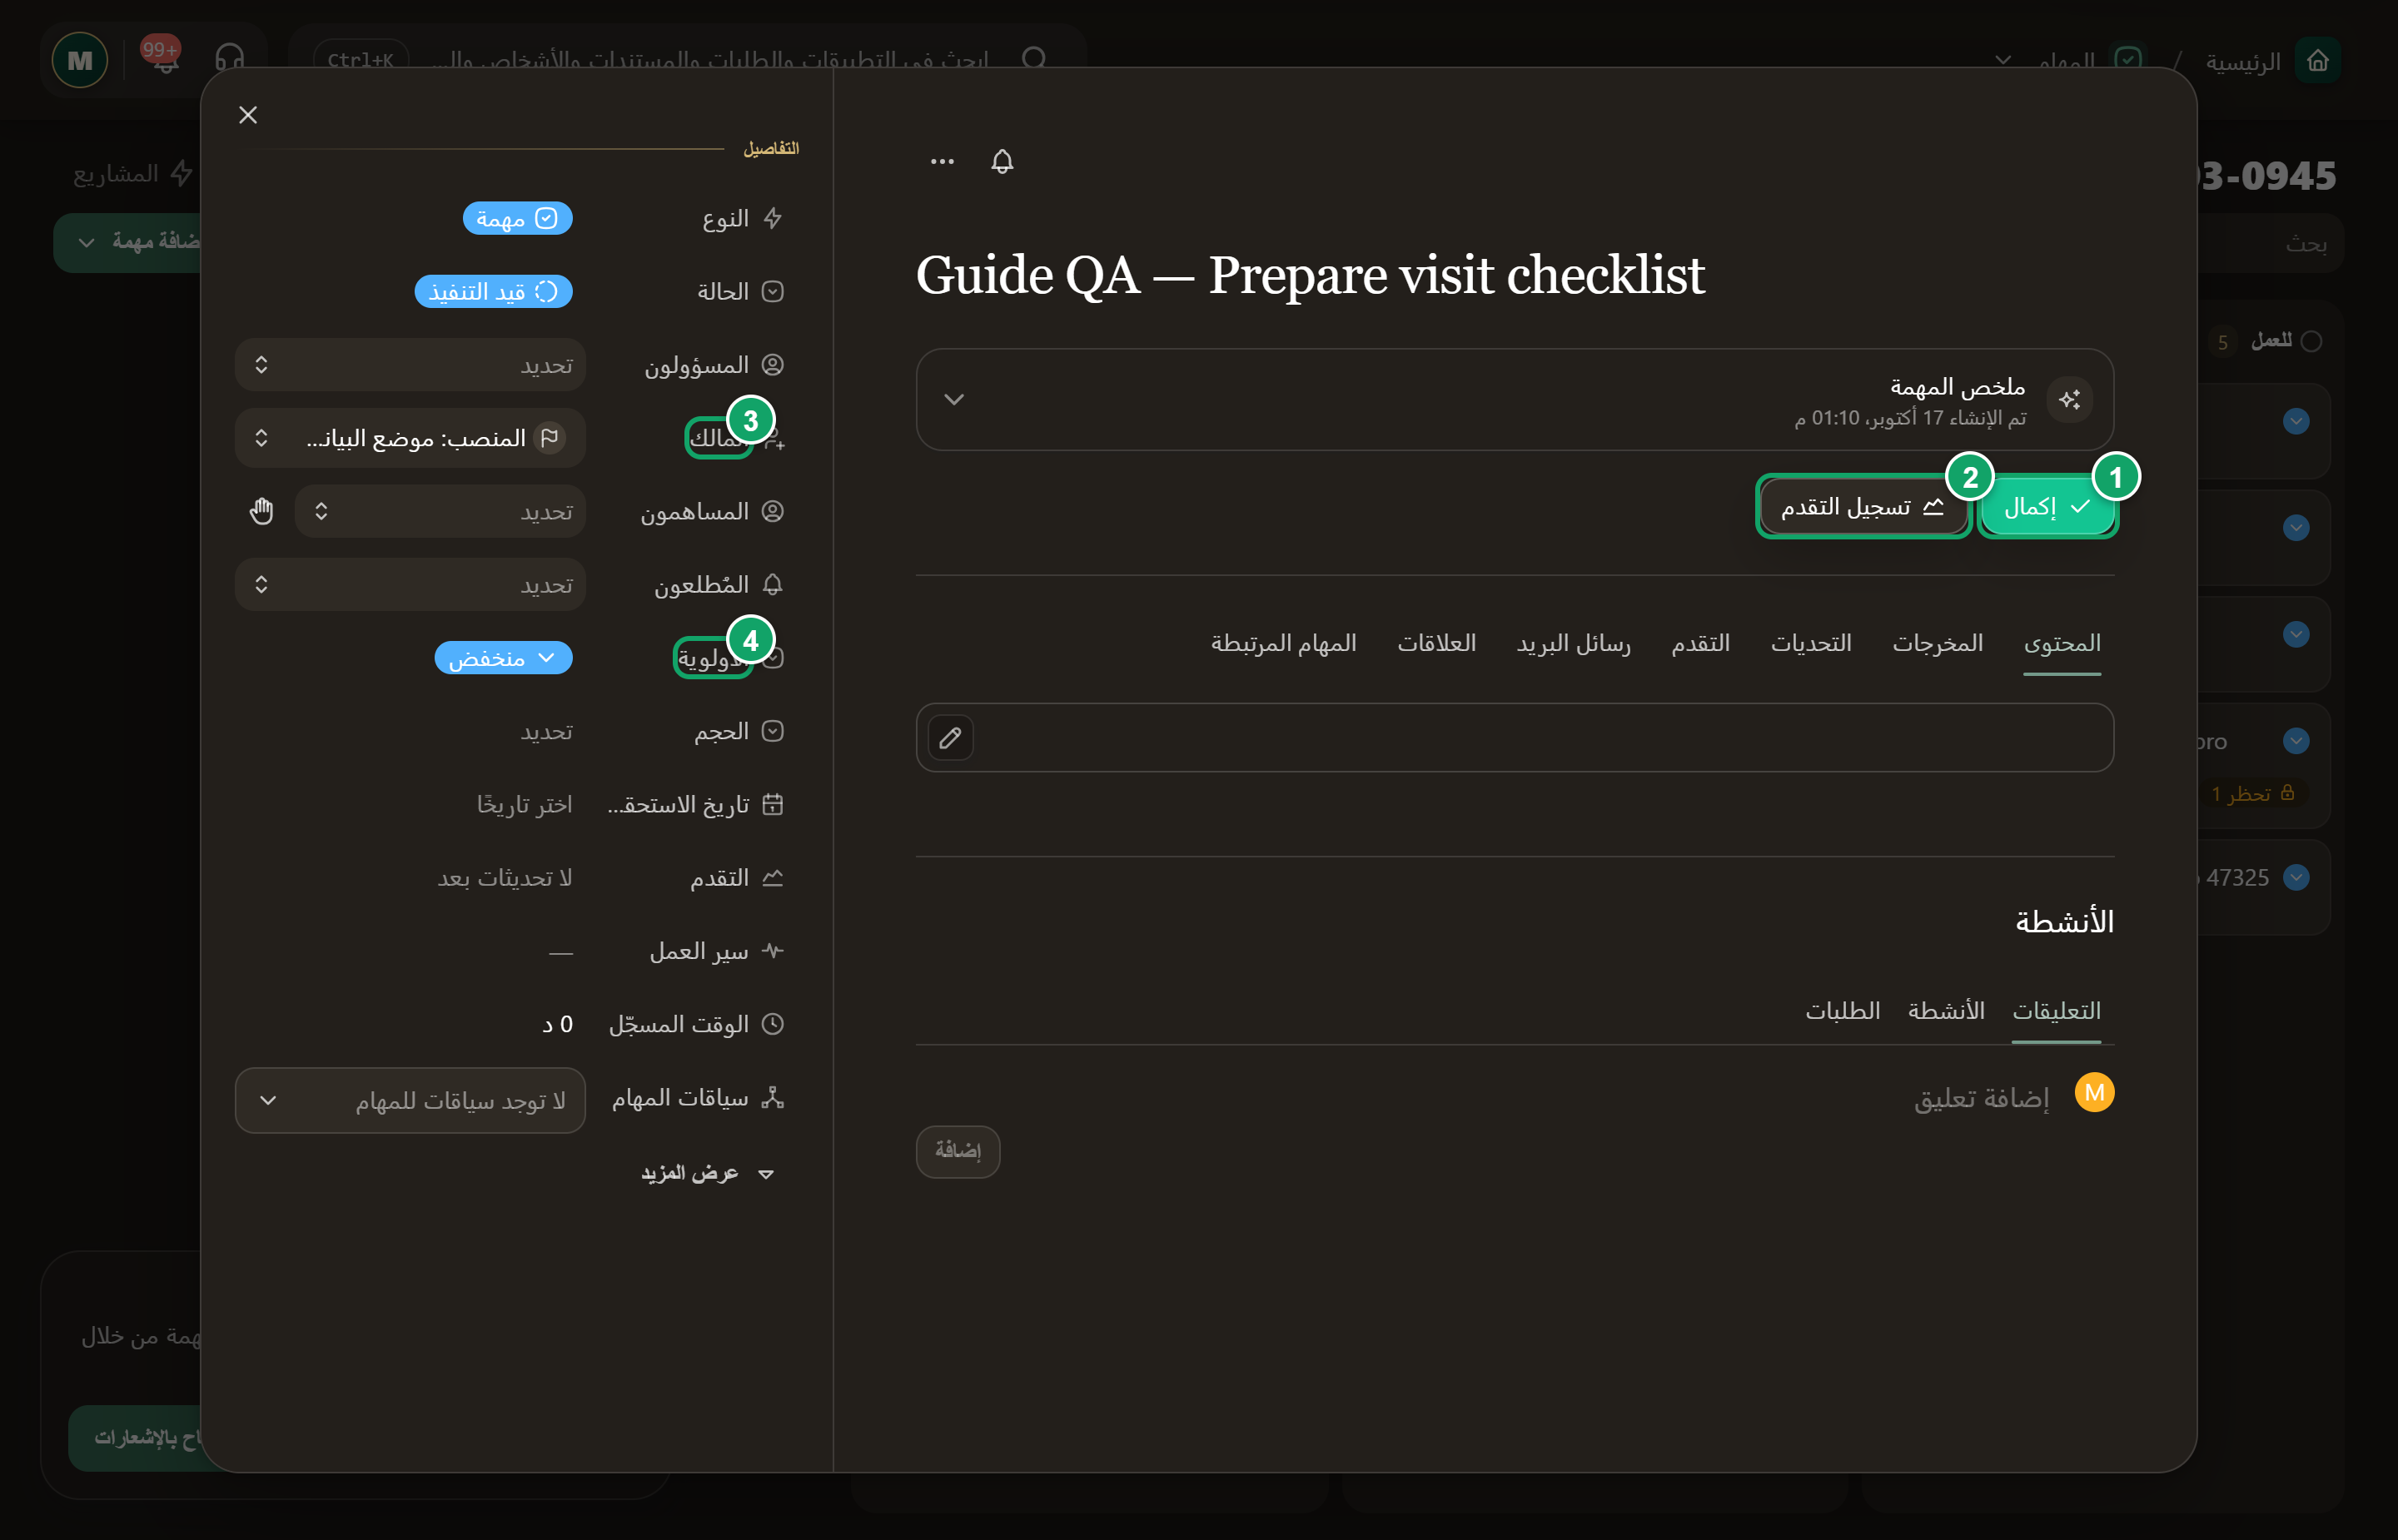
\includegraphics[width=0.95\linewidth,height=0.72\textheight,keepaspectratio]{figures/screens/ch04-details-ar.png}
\caption{تفاصيل مهمة اختبار محفوظة}
\label{fig:tasks-details-details}
\shotnote{تجمع لوحة «التفاصيل» ما يحدد المسؤولية والتخطيط: من ينفّذ، ومن يملك النتيجة، ومن يساهم أو يطّلع، ثم الأولوية والموعد. ويكشف «عرض المزيد» الفئة والمجموعات والمنشئ وتاريخ الإنشاء، ويملأ النظام الأخيرين بنفسه. ولاحظ أن «المالك» قد يكون منصباً لا شخصاً؛ والمهمة الظاهرة مهمة اختبار في test2. ① زر الإجراء الرئيسي، مثل «ابدأ» أو «إكمال». ② «تسجيل التقدم»: ينشر تحديثاً عن العمل. ③ «المالك»: المسؤول عن النتيجة. ④ «الأولوية».}
\end{figure}

\begin{table}[H]
\centering
\caption{ما الذي تجده هنا؟}
\label{tab:tasks-details-data}
\begin{tabularx}{\linewidth}{R{3.6cm} Y}
\rcHeaderRow
\thh{القسم} & \thh{المحتوى والإجراء}\\
العنوان والنوع والحالة & يوضح العنوان النتيجة المطلوبة، ويحدد النوع الإعدادات والقواعد، وتعكس الحالة مرحلة العمل.\\
الأشخاص & يتولى «المسؤولون» التنفيذ، ويُسأل «المالك» عن النتيجة، ويقدّم «المساهمون» جزءاً من العمل، ويحتاج «المطّلعون» إلى المتابعة فقط. وقد تعرض الخيارات أعضاء أو مناصب بحسب الإعداد.\\
التخطيط & الأولوية والحجم وتاريخ الاستحقاق وسياقات المهام. اختر ما يخدم المهمة، فليست كل الروابط إلزامية.\\
عرض المزيد & الفئة و«المشاريع» (المهام الكبرى) والوسوم والمجموعات، إضافة إلى المنشئ وتاريخ الإنشاء اللذين يملؤهما النظام.\\
المحتوى & الوصف والمخرجات والتحديات، ثم التقدم والبريد والعلاقات عند توفرها. وتشرحها الصفحتان التاليتان.\\
المشاركة والحذف & تتيح قائمة المزيد المشاركة عند السماح بها، أو الحذف بعد التأكيد. أكمل المهمة إذا أردت الاحتفاظ بسجل العمل المنجز، لأن الحذف يزيلها.\\
\end{tabularx}
\end{table}

\begin{figure}[H]
\centering
\begin{tikzpicture}[node distance=0.5cm]
\node[stepBox] (a) {\RL{نتيجة واضحة}};
\node[stepBox,below=of a] (b) {\RL{مسؤولية وموعد}};
\node[stepBox,below=of b] (c) {\RL{إنشاء ثم تحقق}};
\draw[flowsTo] (a) -- (b);
\draw[flowsTo] (b) -- (c);
\end{tikzpicture}
\rclegend
\caption{خطوات الاستخدام}
\label{fig:tasks-details-flow}
\shotnote{يرتب المخطط إنشاء المهمة في ثلاث خطوات: صياغة النتيجة المطلوبة، ثم تحديد من يتولاها ومتى، ثم الإنشاء والتحقق. فالعنوان الواضح يسهّل اختيار المسؤول المناسب، وإعادة فتح المهمة بعد إنشائها تؤكد أن بياناتها حُفظت كما أردت.}
\end{figure}

\subsection{خطوات العمل والتحقق}
\begin{enumerate}
\item اختر «إضافة مهمة» ثم النوع المتاح. اكتب عنواناً يصف النتيجة، وأضف الوصف.
\item حدد المسؤولين عن التنفيذ والمالك، والموعد والأولوية عند الحاجة، وراجع العلاقات المطلوبة قبل الإنشاء.
\item اضغط «إنشاء»، ثم افتح المهمة من القائمة أو اللوحة وتحقق من العنوان والمسؤولية والحالة.
\item بعد تعديل أي حقل في المهمة المحفوظة، انتظر تأكيد الحفظ. أما في محرر النص فاستخدم إجراء الحفظ، ثم أعد فتح المهمة للتأكد.
\end{enumerate}

\textbf{تحقق ومعالجة المشكلة:} إذا تعذّر الحفظ، فراجع رسالة الخطأ والنوع والعلاقات المطلوبة وصلاحيتك. ولا تفترض أن النص حُفظ لمجرد إغلاق النافذة.

\clearpage
\section{التقدم والنتائج والتواصل}
\label{sec:tasks-feature-follow-up}

تجمع المهمة ما أُنجز وما يعيق العمل وما يحتاجه أفراد الفريق بعضهم من بعض. حدّث النتيجة والحالة باستمرار حتى يتابع زميلك العمل دون تخمين.

\textbf{المسار ومن يستخدمه:} افتح مهمة محفوظة، واستخدم تبويبات المحتوى وقسم «الأنشطة». يستخدمها المنفّذ والمساهم والمسؤول عن النتيجة.

\begin{rcnote}[مثال: شركة الأفق]
يسجّل عمر ما أعدّه لقائمة الزيارة، ويوضح أن عنوان الموقع لم يصل بعد، فتراجع سارة العائق وتحدد الخطوة التالية.
\end{rcnote}

\begin{figure}[H]
\centering
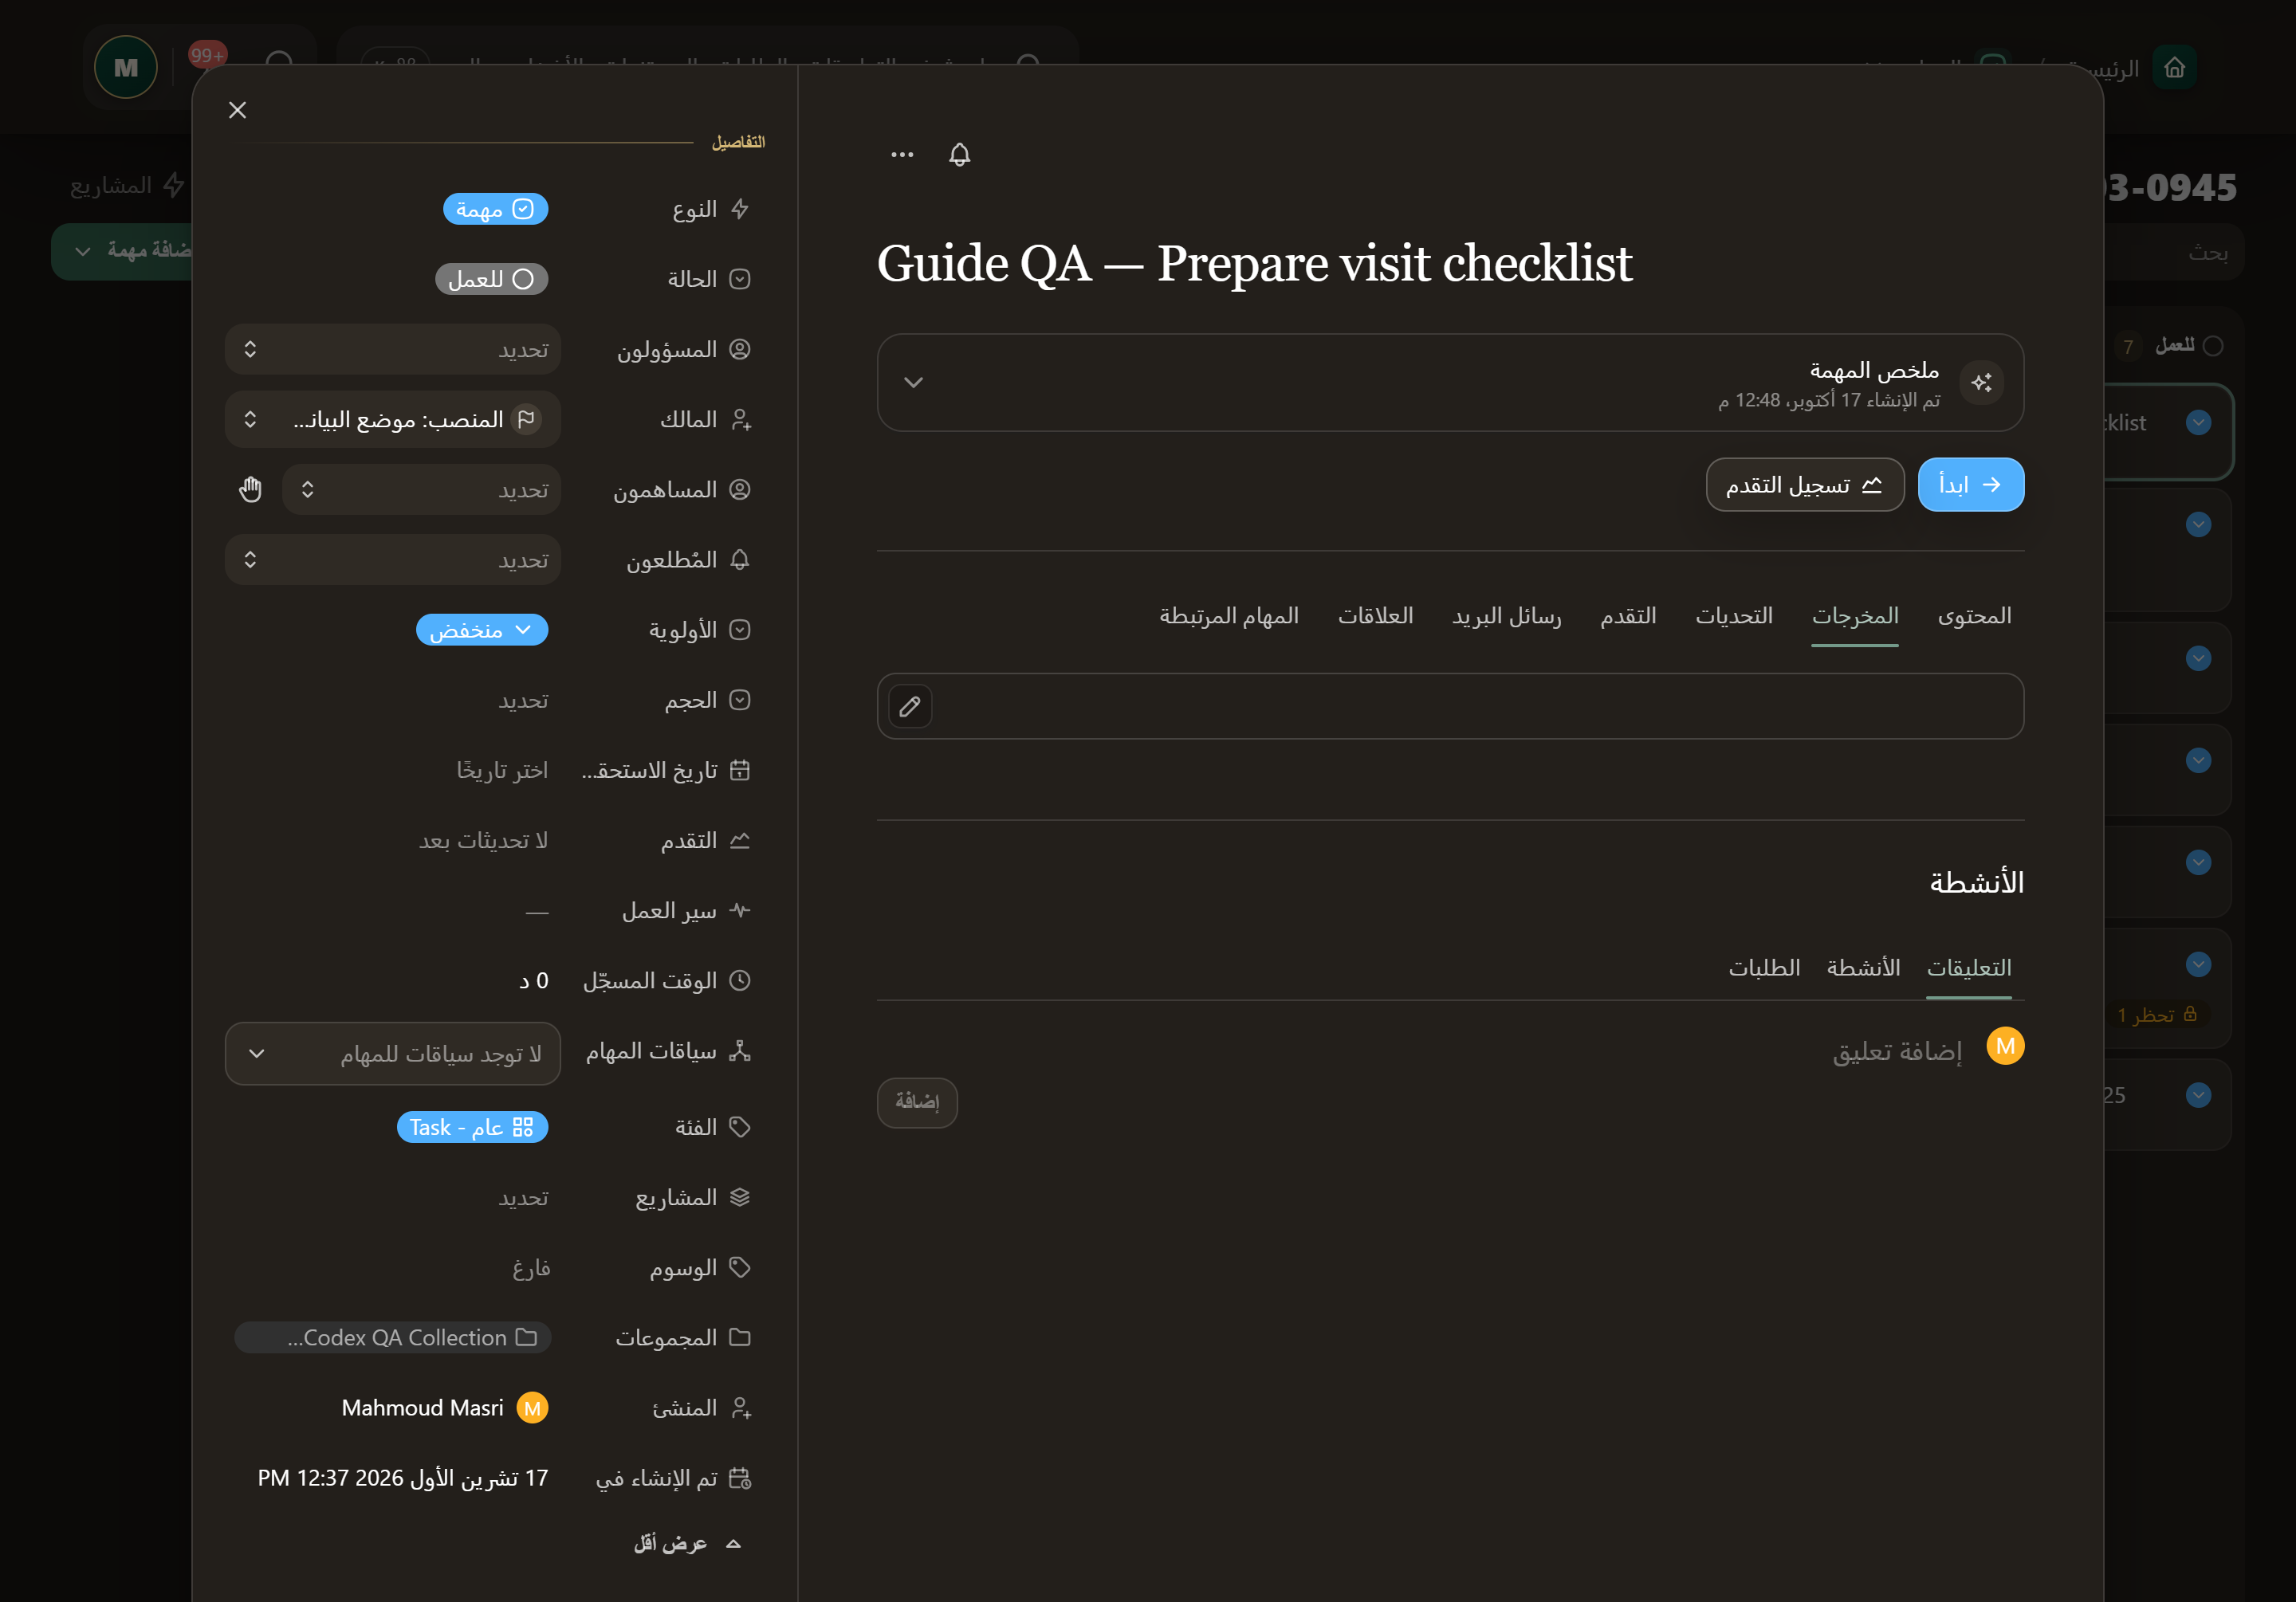
\includegraphics[width=0.95\linewidth,height=0.72\textheight,keepaspectratio]{figures/screens/ch04-output-ar.png}
\caption{المخرجات}
\label{fig:tasks-follow-up-output}
\shotnote{تبويب «المخرجات» هو المكان الذي تسجّل فيه ما نتج عن العمل فعلاً، بعد الضغط على أيقونة التعديل. وبذلك يفصل الفريق بين وصف المطلوب في «المحتوى» والنتيجة المنجزة هنا. ويبقى التبويب فارغاً، كما في هذه المهمة التجريبية، حتى يكتب المنفّذ نتيجته. ① تبويب «المخرجات» داخل المهمة. ② زر الإجراء الرئيسي للمهمة، مثل «ابدأ» أو «إكمال»، ويتغير بحسب حالتها. واكتب في التبويب النتيجة الفعلية للعمل.}
\end{figure}

\begin{figure}[H]
\centering
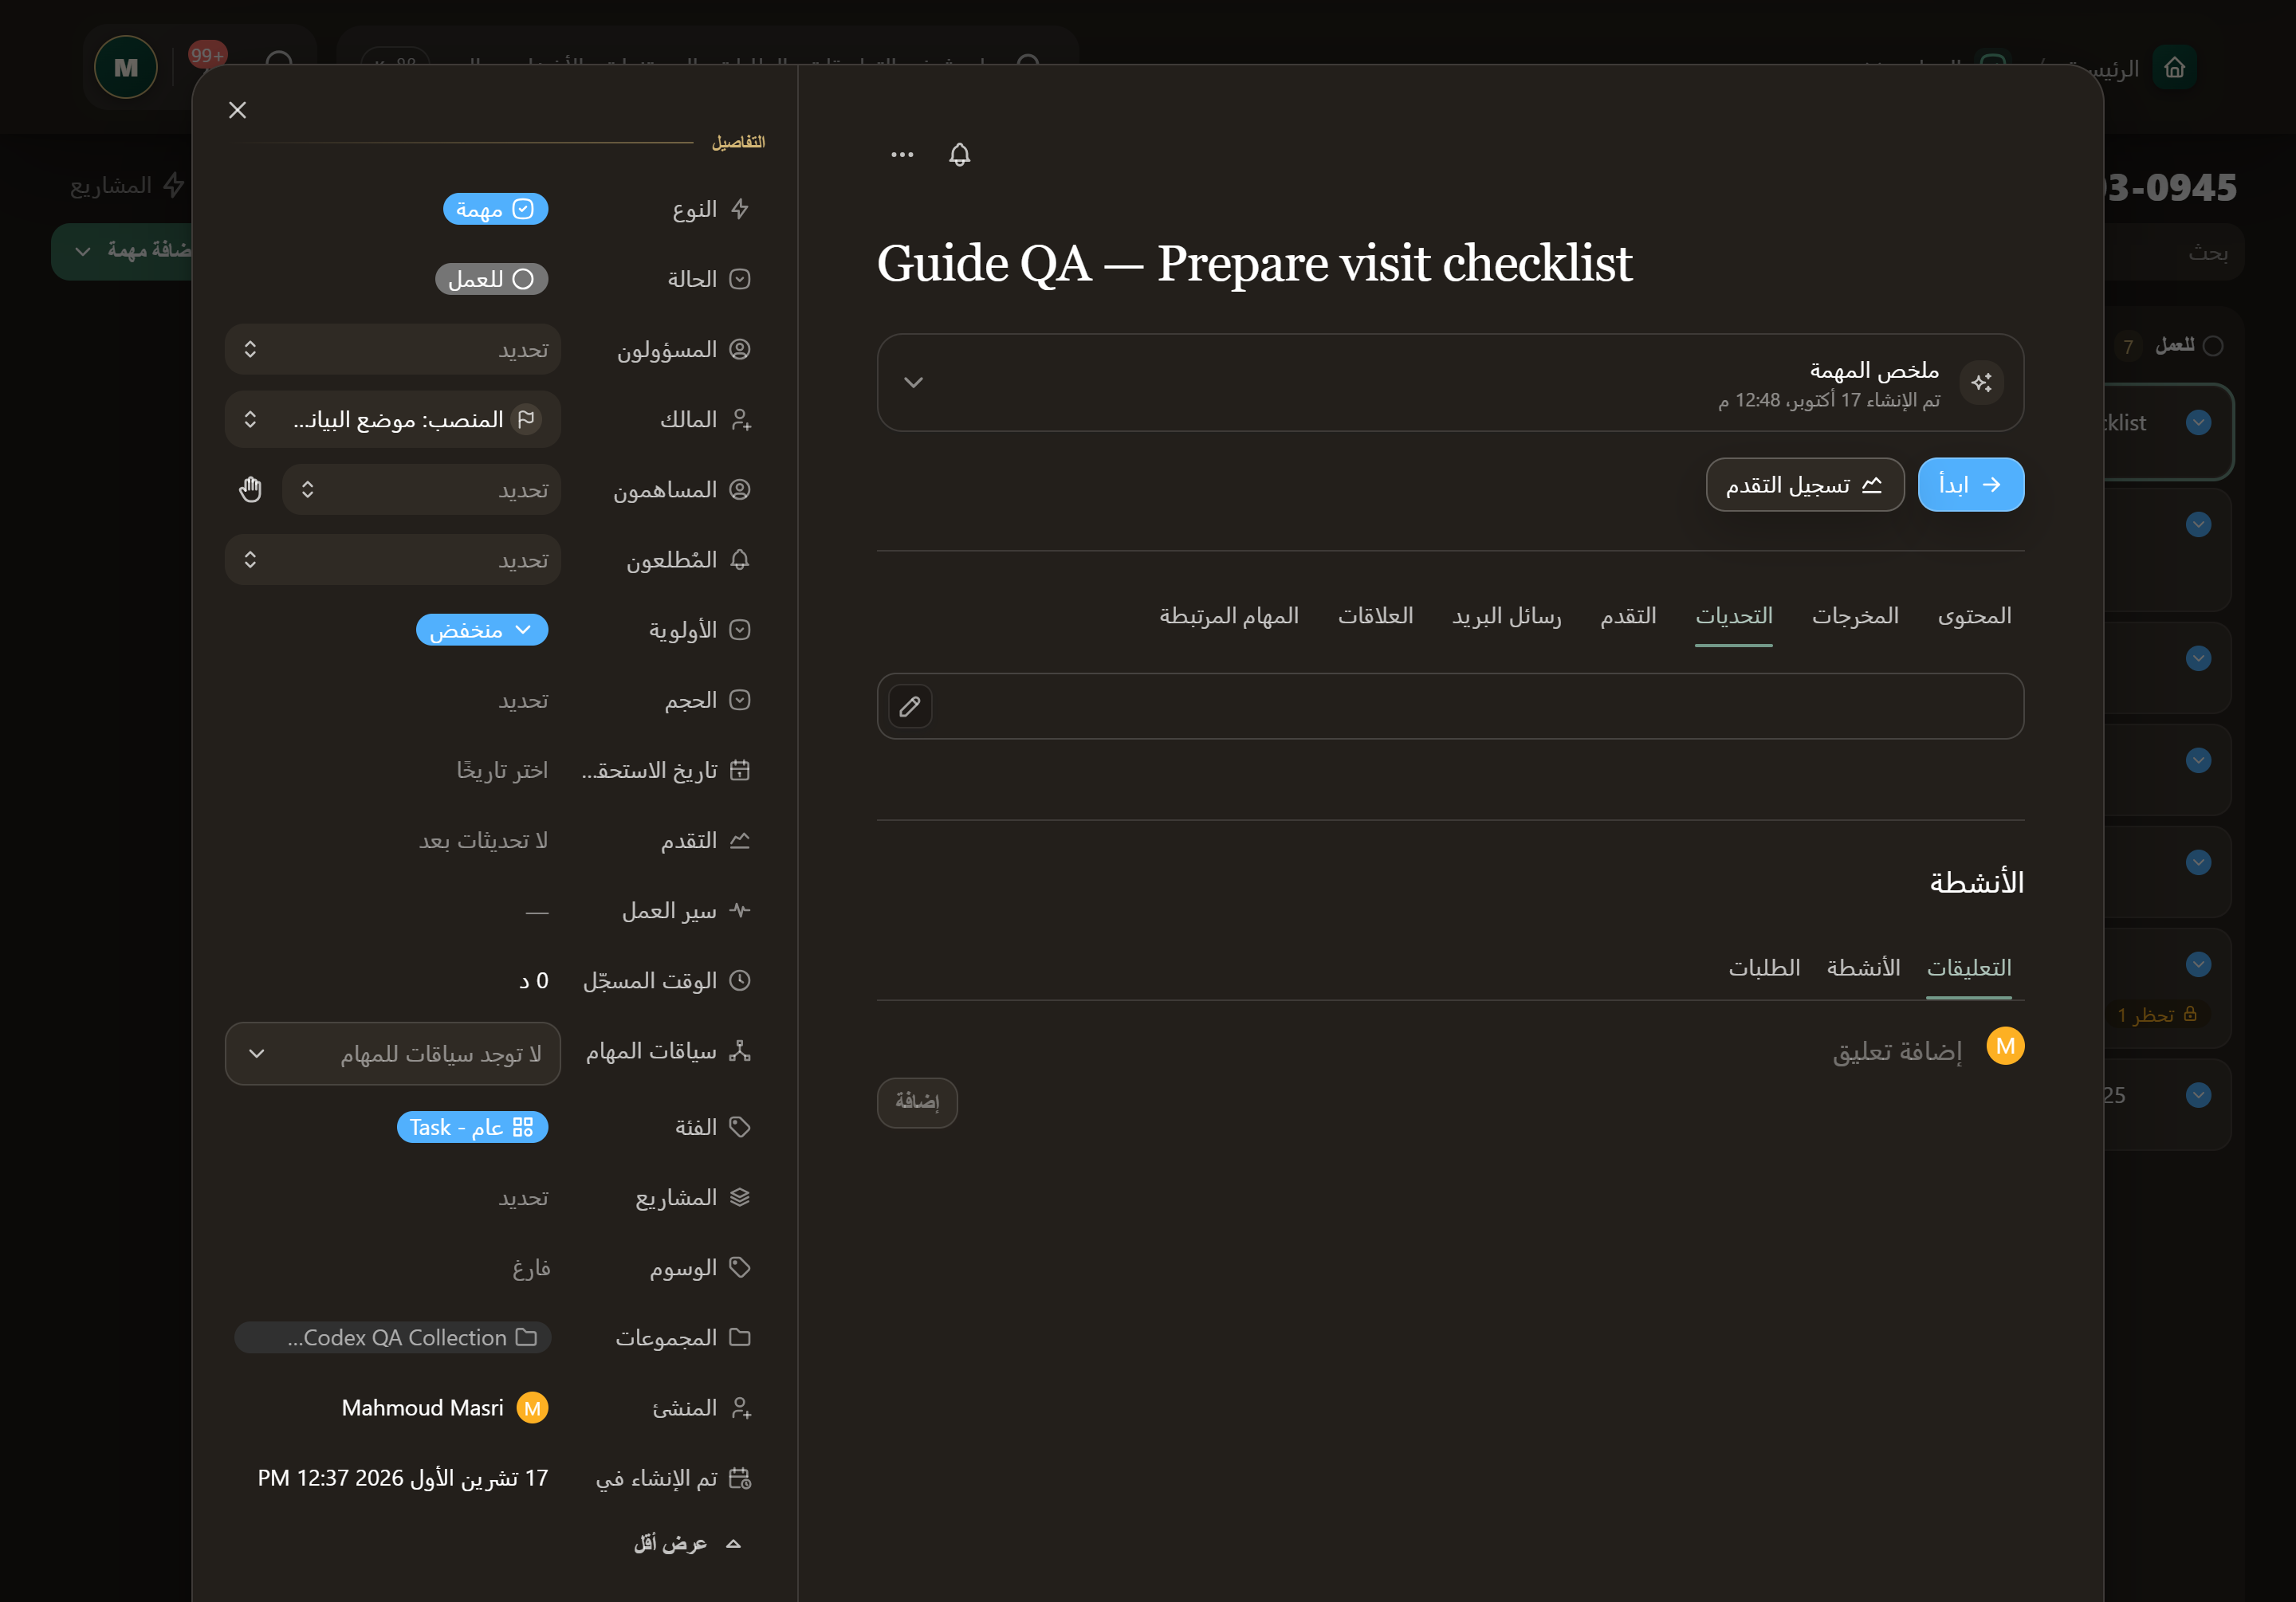
\includegraphics[width=0.95\linewidth,height=0.72\textheight,keepaspectratio]{figures/screens/ch04-challenges-ar.png}
\caption{التحديات}
\label{fig:tasks-follow-up-challenges}
\shotnote{يخصَّص تبويب «التحديات» للعوائق التي تؤخر العمل أو تحتاج قراراً من شخص آخر، وهو فارغ في هذه المهمة التجريبية. ويُطلع تسجيلُ العائق هنا الفريقَ عليه، لكنه لا يغيّر حالة المهمة تلقائياً؛ لذلك غيّر الحالة أو اطلب المساعدة بإجراء مستقل. ① تبويب «التحديات» داخل المهمة. ② زر الإجراء الرئيسي للمهمة، مثل «ابدأ» أو «إكمال»، ويتغير بحسب حالتها. واكتب في التبويب ما يعيق العمل.}
\end{figure}

\begin{figure}[H]
\centering
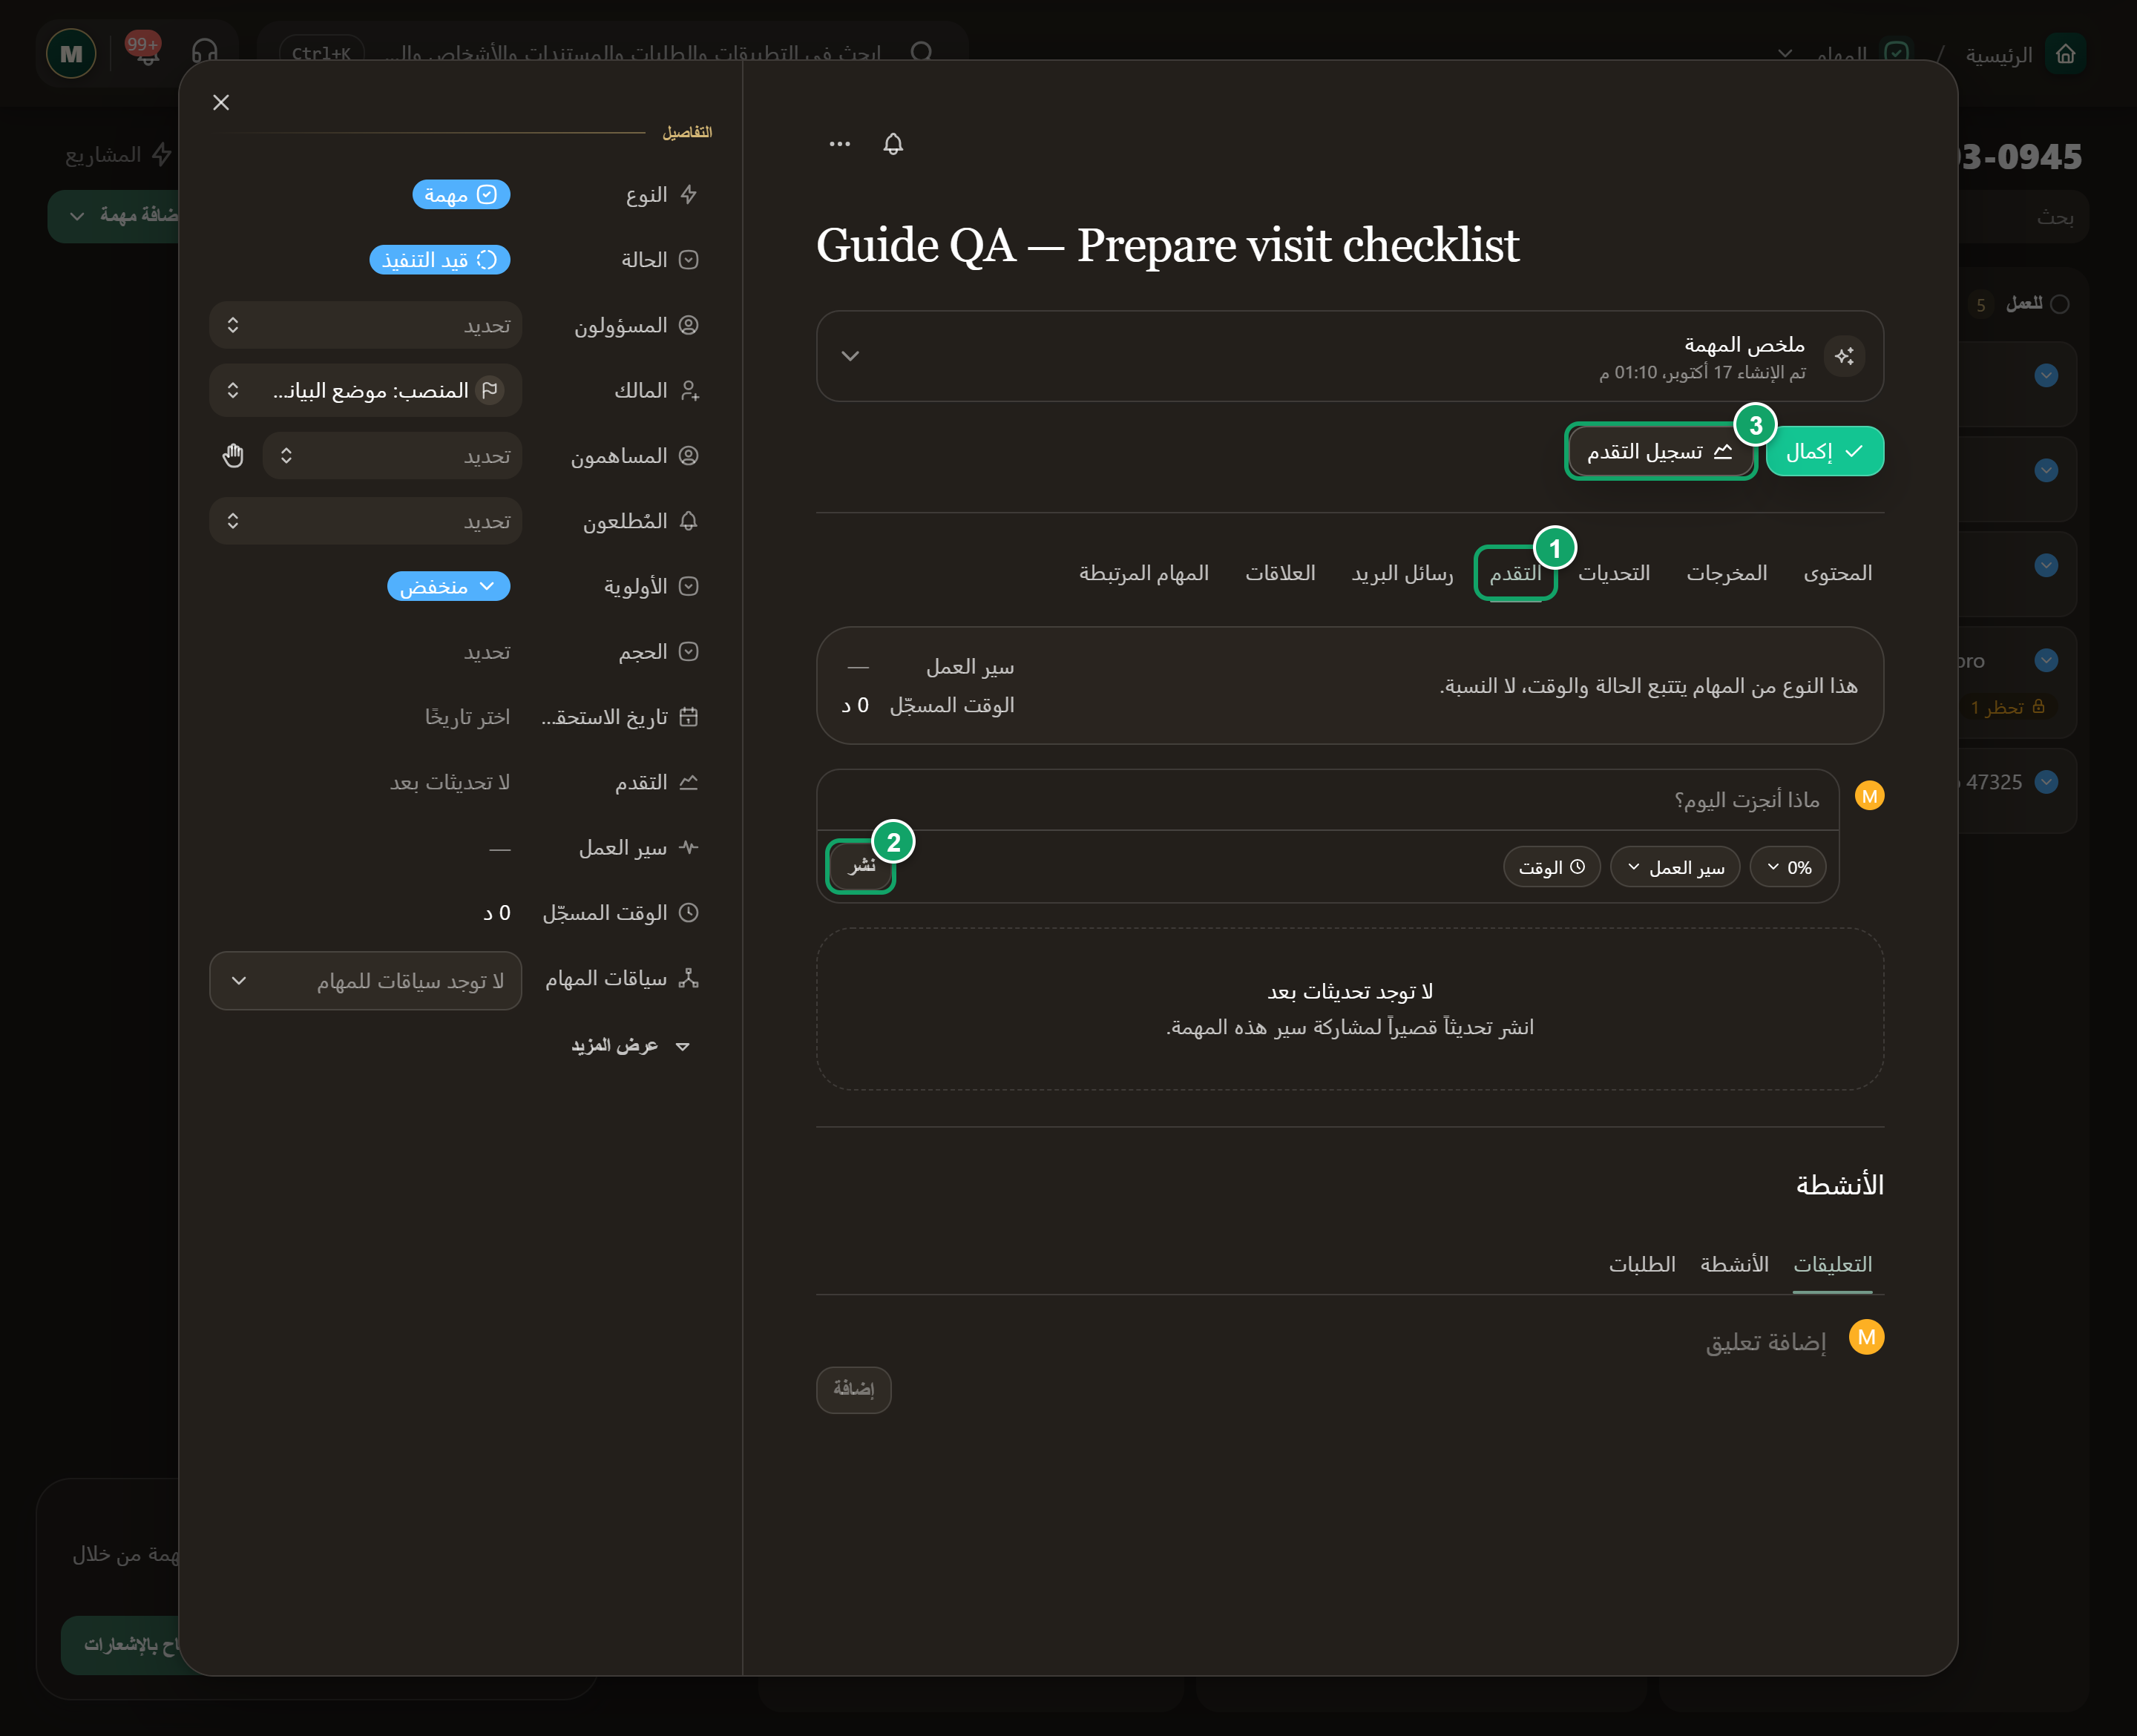
\includegraphics[width=0.95\linewidth,height=0.72\textheight,keepaspectratio]{figures/screens/ch04-progress-ar.png}
\caption{تحديثات التقدم}
\label{fig:tasks-follow-up-progress}
\shotnote{يجمع تبويب «التقدم» التحديثات القصيرة التي ينشرها الفريق عن سير المهمة: تكتب في «ماذا أنجزت اليوم؟» ثم تضغط «نشر». ويحدد نوع المهمة ما يُتتبَّع، فنوع هذه المهمة مثلاً يتتبع الحالة والوقت لا النسبة. ولا توجد تحديثات بعد في هذه المهمة التجريبية. ① تبويب «التقدم». ② «نشر»: يرسل التحديث بعد كتابة ما أنجزته والنسبة وسير العمل. ③ «تسجيل التقدم»: يفتح التحديث من أعلى المهمة.}
\end{figure}

\begin{figure}[H]
\centering
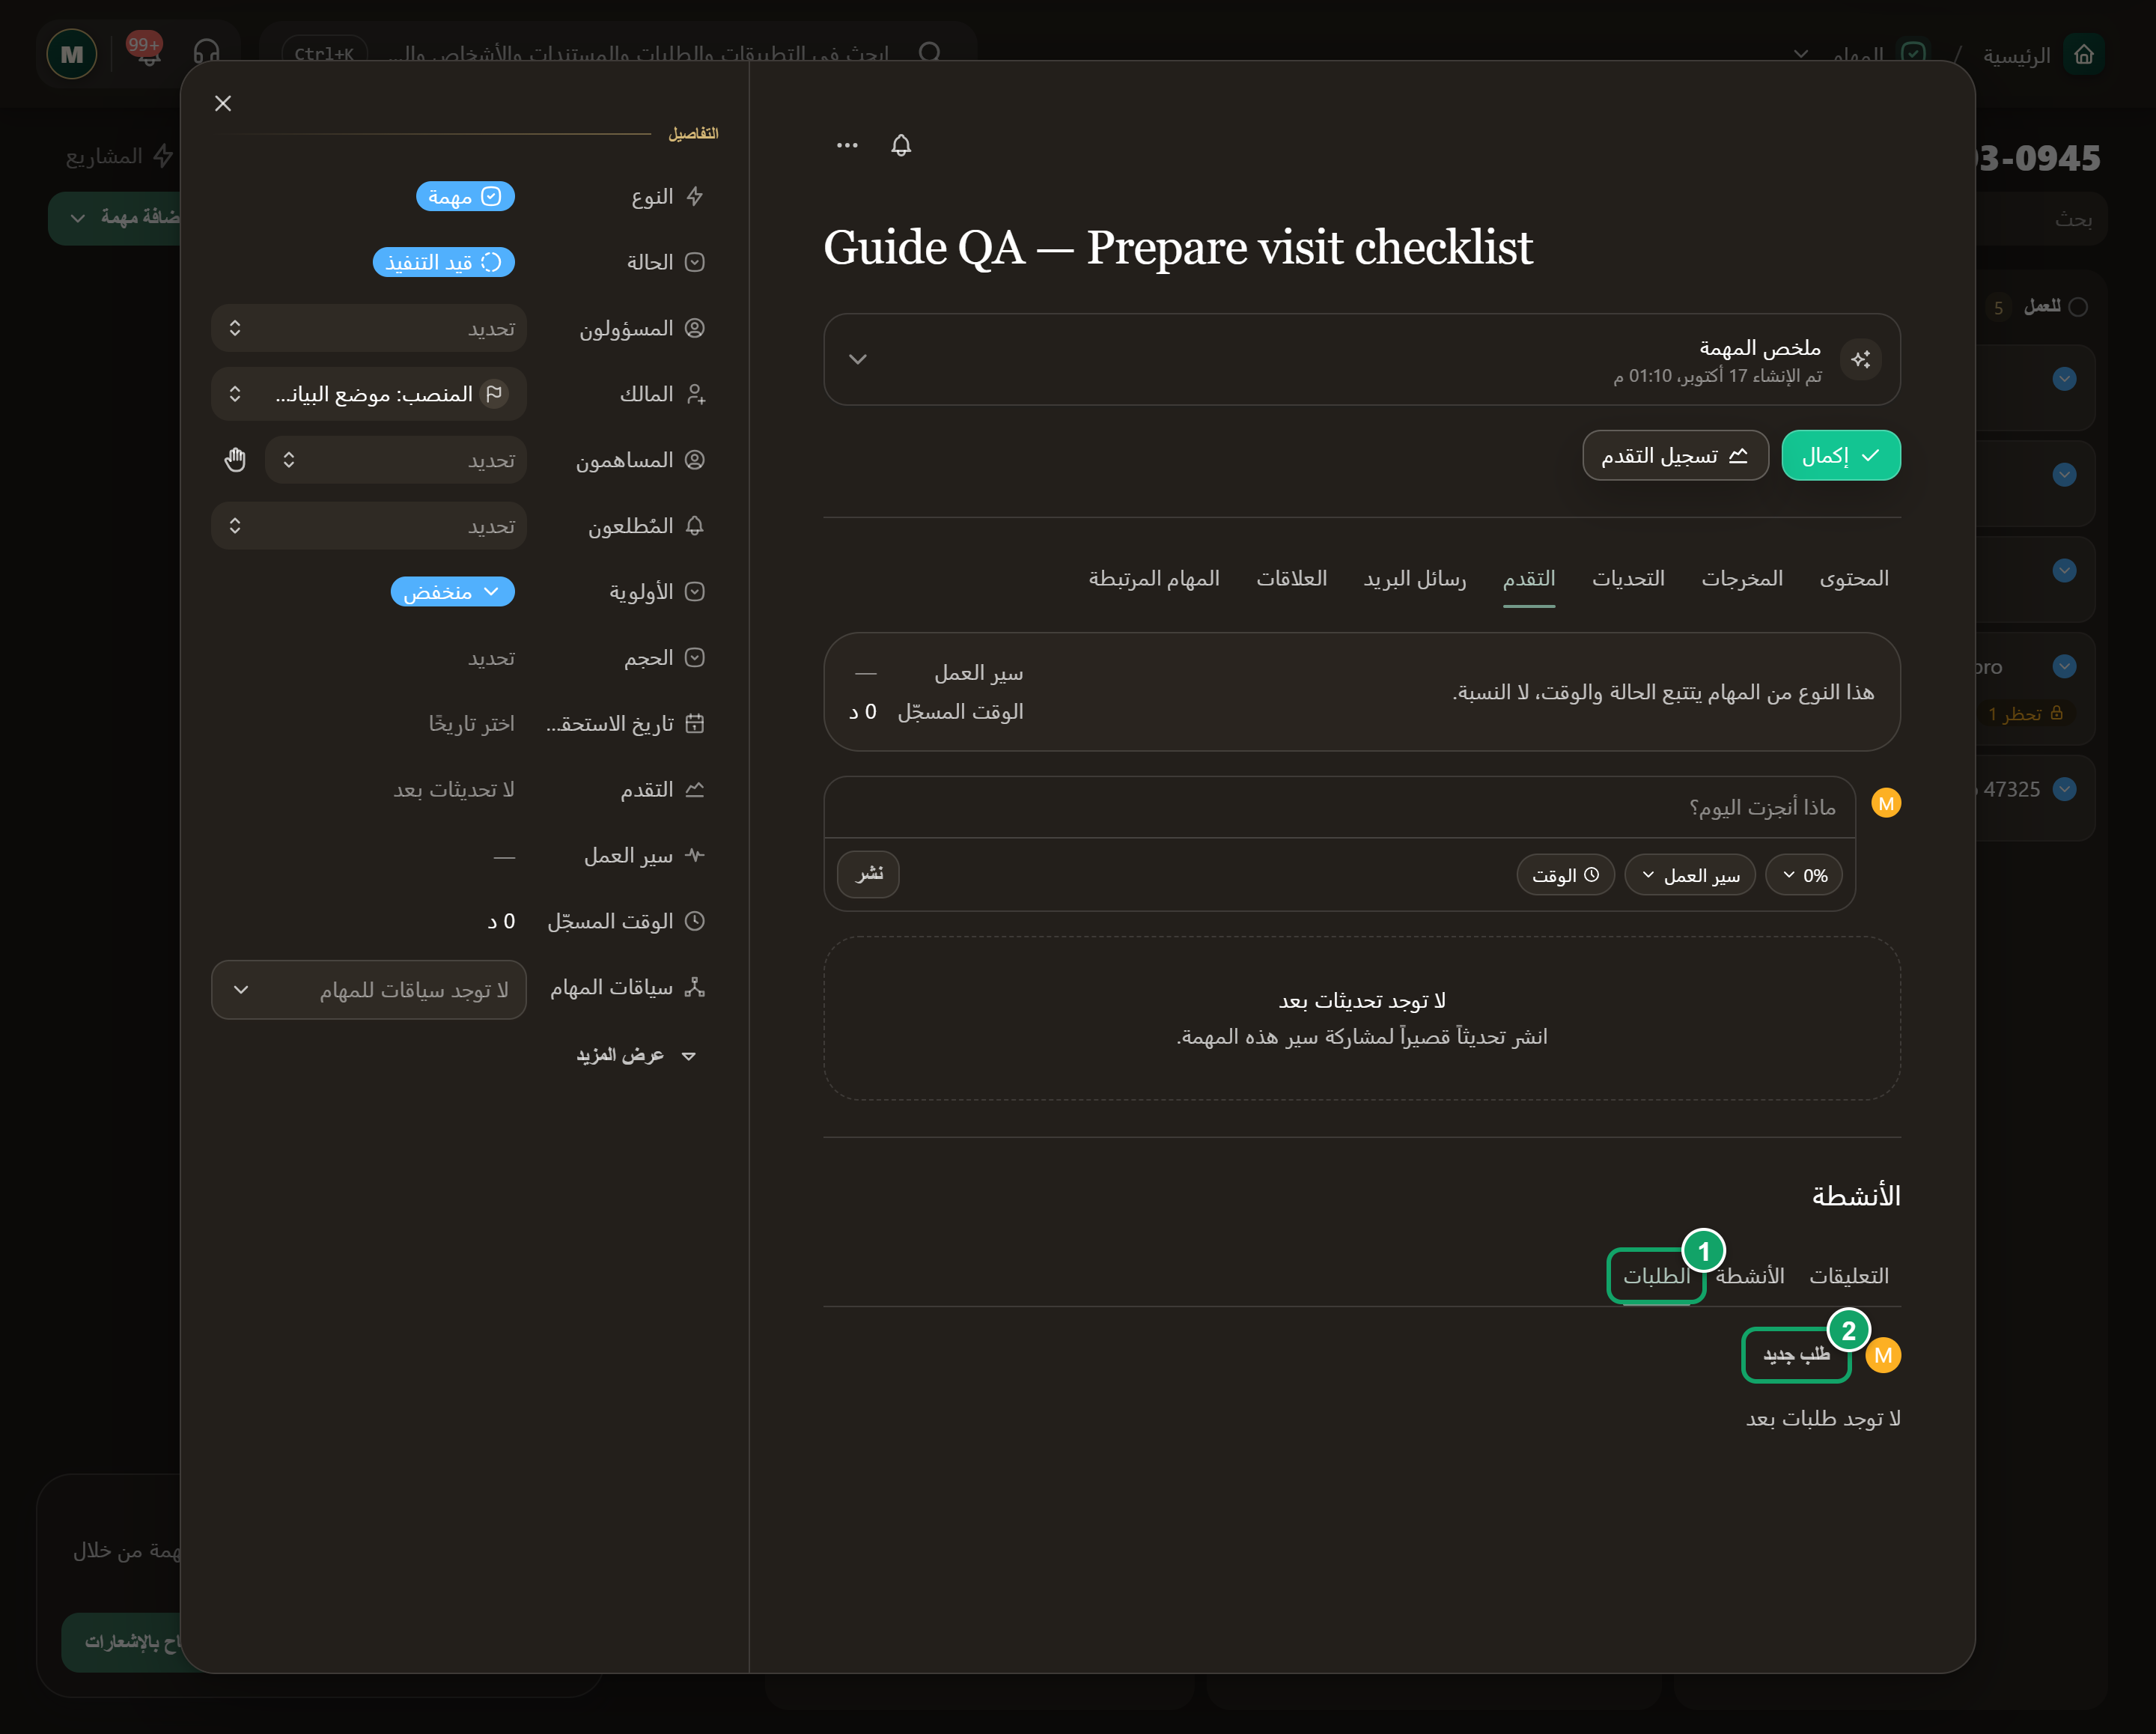
\includegraphics[width=0.95\linewidth,height=0.72\textheight,keepaspectratio]{figures/screens/ch04-requests-ar.png}
\caption{الطلبات داخل المهمة}
\label{fig:tasks-follow-up-requests}
\shotnote{تتيح «الطلبات» أن تطلب من عضو آخر إجراءً محدداً داخل سجل المهمة نفسه عبر «طلب جديد»، فيبقى الطلب ورده مرتبطين بالعمل بدلاً من ضياعهما في المراسلات. وحالة الطلب مستقلة عن حالة المهمة، ولا توجد طلبات في هذه المهمة التجريبية. ① تبويب «الطلبات». ② «طلب جديد»: يطلب من زميل عملاً أو معلومة مرتبطة بالمهمة.}
\end{figure}

\begin{figure}[H]
\centering
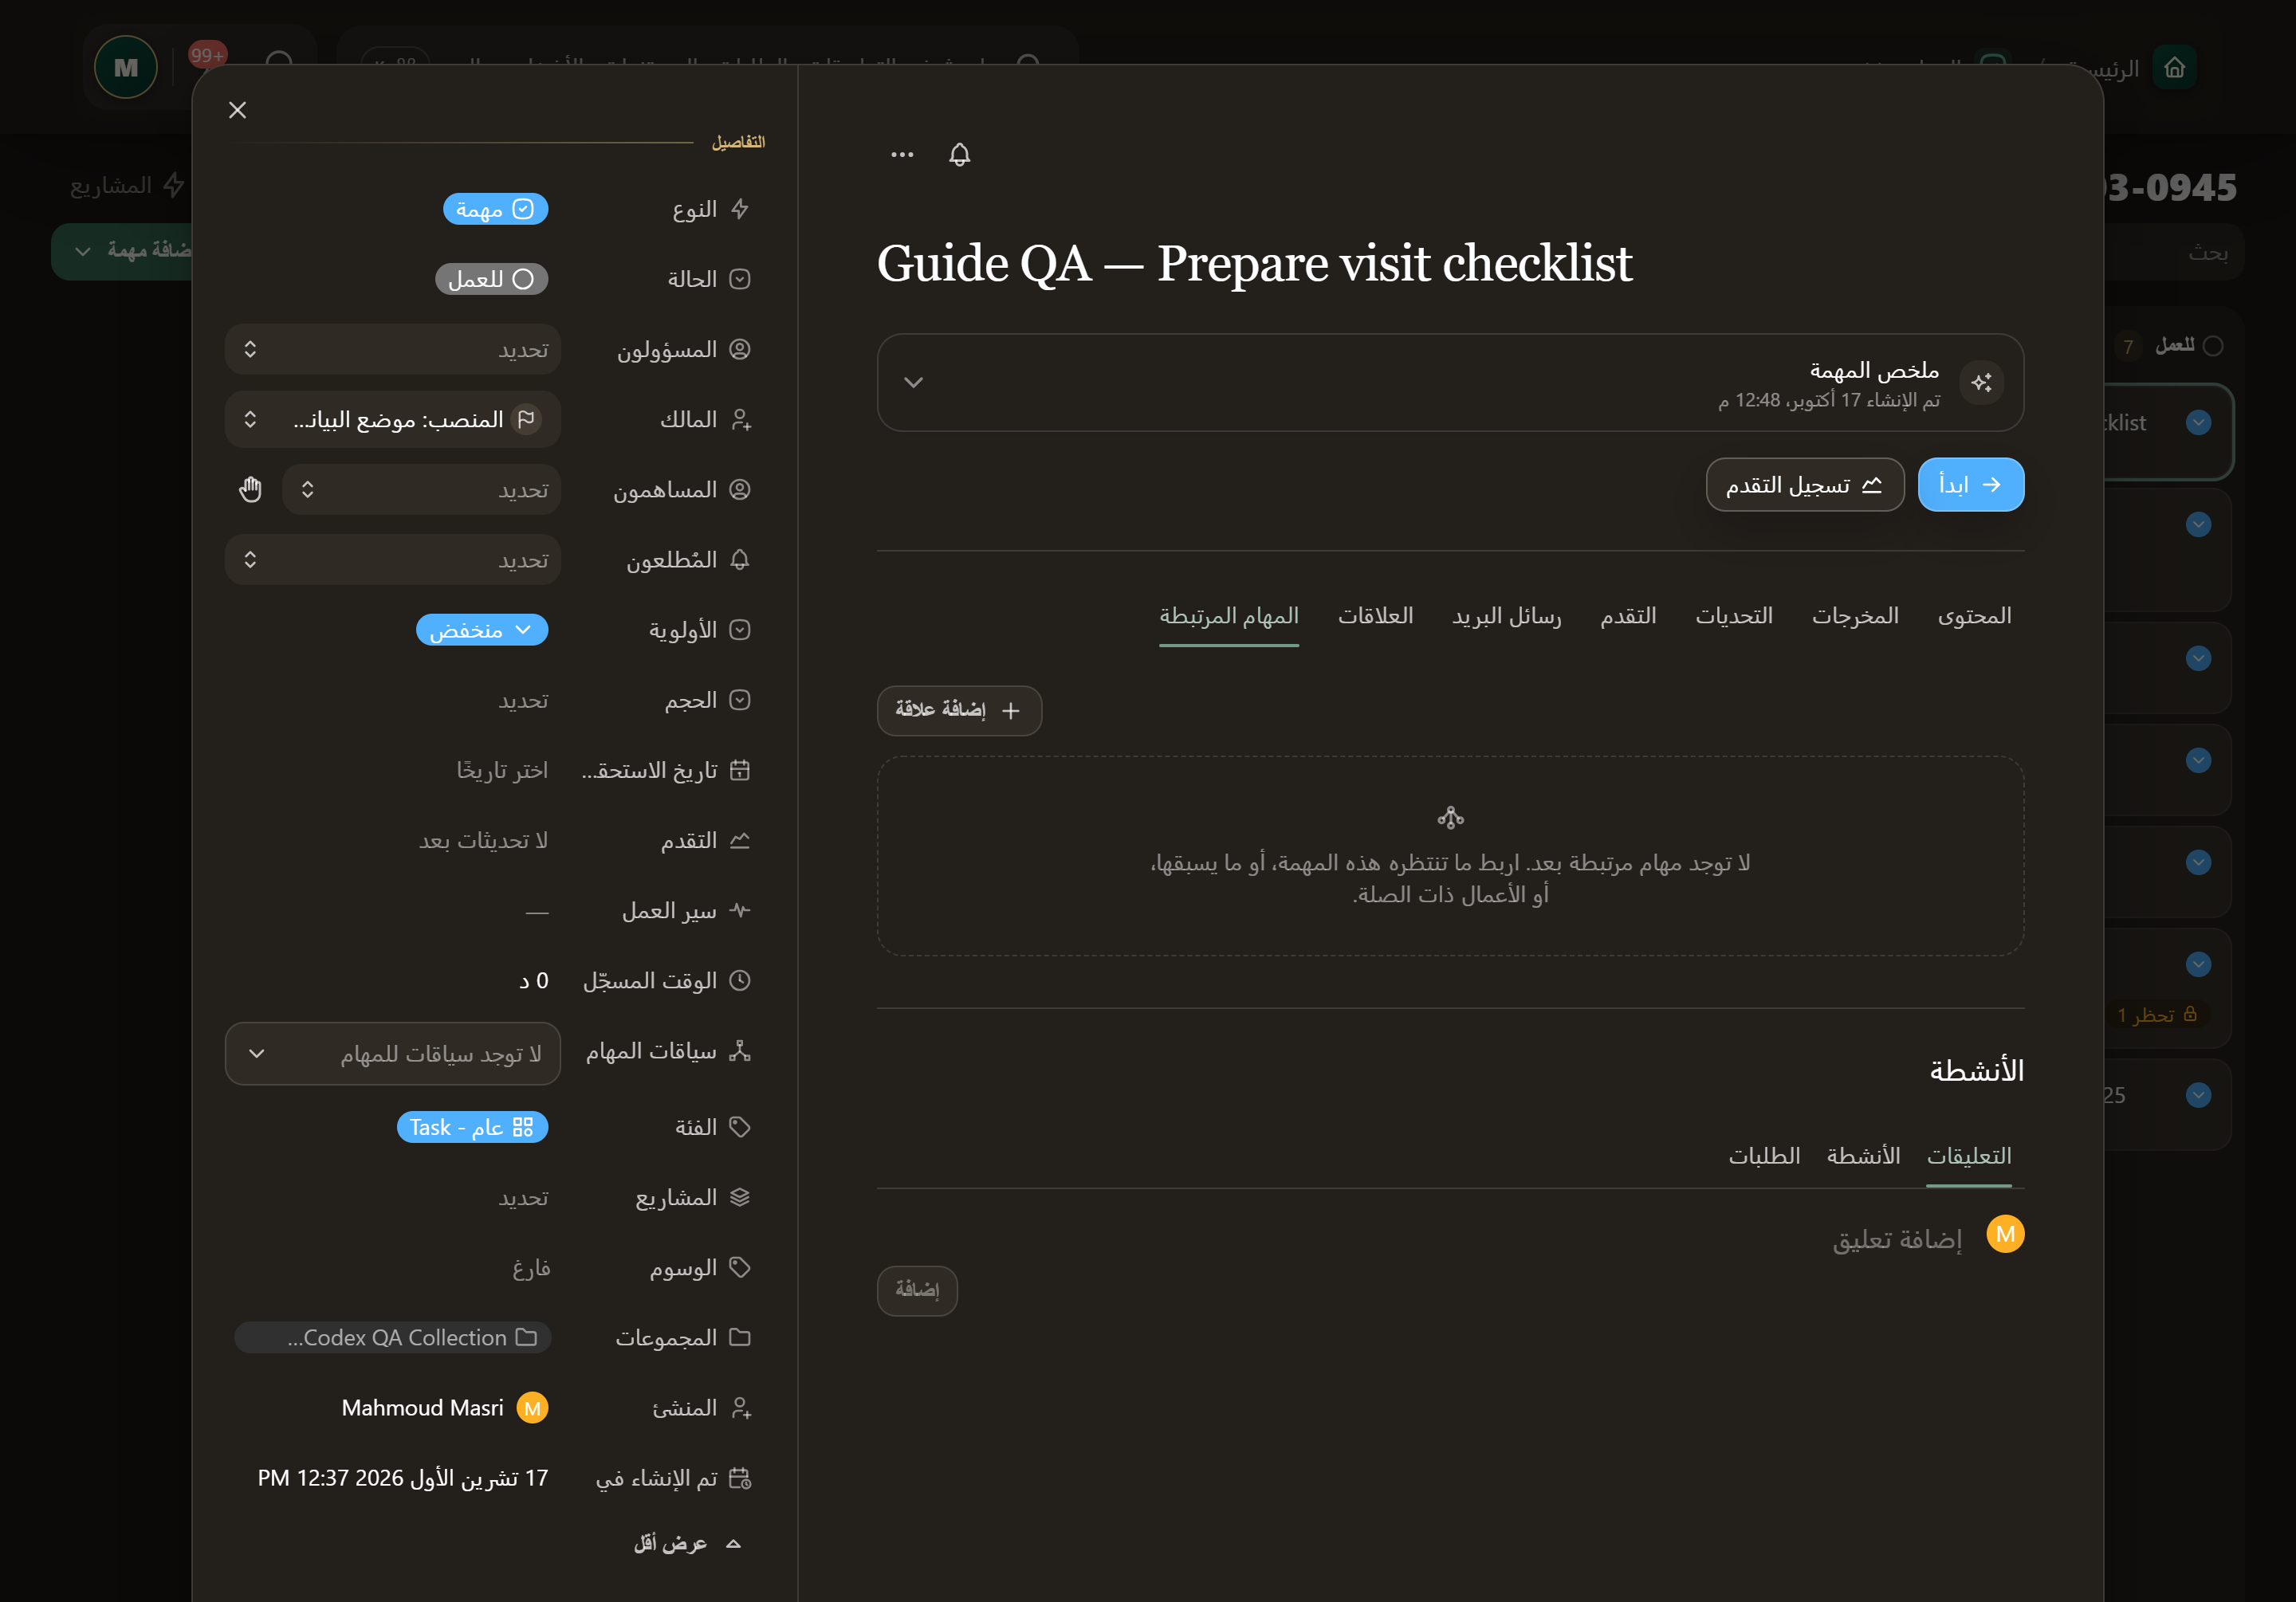
\includegraphics[width=0.95\linewidth,height=0.72\textheight,keepaspectratio]{figures/screens/ch04-comments-ar.png}
\caption{التعليقات}
\label{fig:tasks-follow-up-comments}
\shotnote{تجمع «التعليقات» نقاش الفريق حول المهمة: اكتب في «إضافة تعليق» ثم اضغط «إضافة». ويفيد التعليق في شرح القرارات وطرح الأسئلة، لكنه لا يغيّر حالة المهمة ولا يغني عن تسجيل النتيجة في «المخرجات». ① تبويب «التعليقات». ② «إضافة».}
\end{figure}

\begin{figure}[H]
\centering
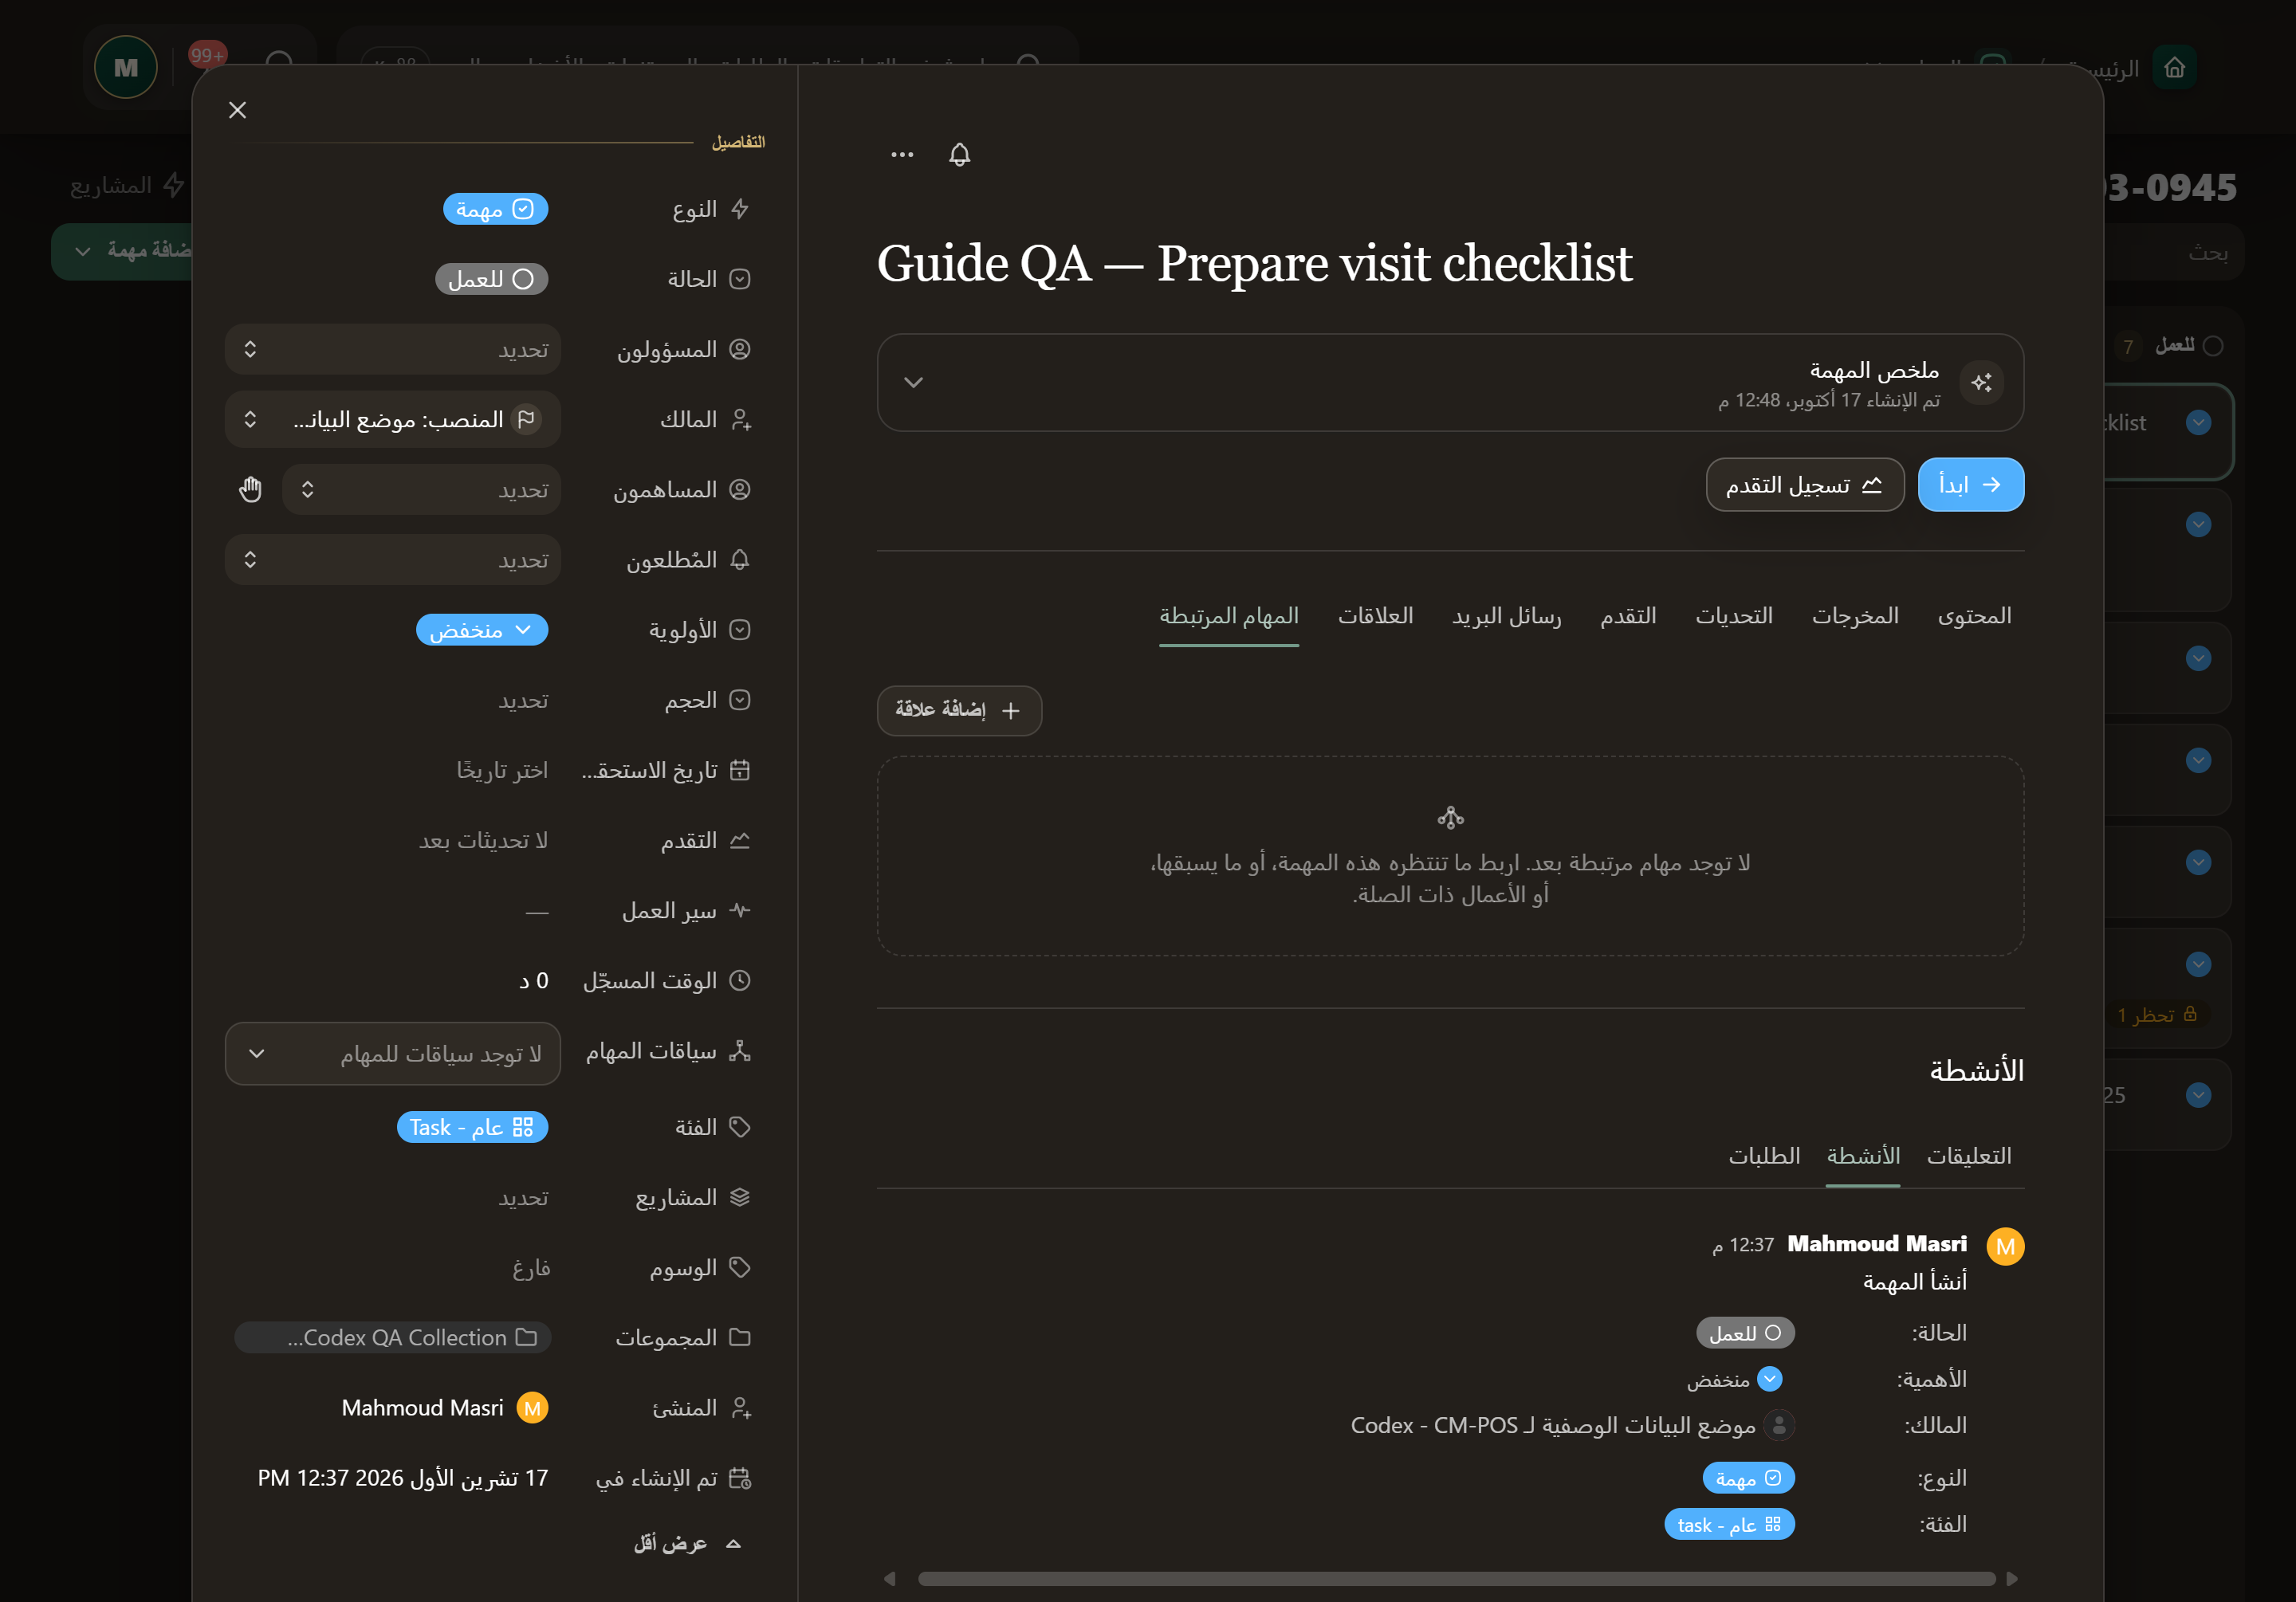
\includegraphics[width=0.95\linewidth,height=0.72\textheight,keepaspectratio]{figures/screens/ch04-activity-ar.png}
\caption{سجل الأنشطة}
\label{fig:tasks-follow-up-activity}
\shotnote{يعرض تبويب «الأنشطة» سجلاً زمنياً لما جرى على المهمة ومن قام به؛ فهنا يظهر حدث «أنشأ المهمة» مع قيمها الأولى مثل الحالة والمالك والنوع. ويرجع إليه المسؤول عندما يسأل عن تغيير ما، أما نتيجة العمل فتُكتب في «المخرجات» لا هنا. الرقم في الصورة: ① تبويب «الأنشطة» الذي يسجّل كل تغيير على المهمة ومن أجراه ومتى.}
\end{figure}

\begin{table}[H]
\centering
\caption{ما الذي تجده هنا؟}
\label{tab:tasks-follow-up-data}
\begin{tabularx}{\linewidth}{R{3.6cm} Y}
\rcHeaderRow
\thh{القسم} & \thh{المحتوى والإجراء}\\
الوصف والمخرجات والتحديات & سياق التنفيذ، ثم نتيجته، ثم عوائقه. ويدعم محرر المحتوى الملفات حيث تتوفر أدوات الإرفاق.\\
التقدم & تحديثات مؤرخة، ونسبة الإنجاز، و«سير العمل»، والوقت، والخطوات التالية، والعوائق؛ بحسب إعداد النوع.\\
التعليقات والأنشطة & نقاش العمل وسجل التغييرات. ويتيح لك زر المتابعة أن تتابع المهمة أو تلغي متابعتها.\\
الطلبات والملخص & طلب مساهمة أو رد من عضو آخر، وحالة الطلب مستقلة عن حالة المهمة. أما «ملخص المهمة» المساعد فيحتاج إلى مراجعة ولا يحل محل السجل.\\
\end{tabularx}
\end{table}

\begin{figure}[H]
\centering
\begin{tikzpicture}[node distance=0.5cm]
\node[stepBox] (a) {\RL{تسجيل النتيجة}};
\node[stepBox,below=of a] (b) {\RL{معالجة العائق}};
\node[stepBox,below=of b] (c) {\RL{مراجعة الحالة}};
\draw[flowsTo] (a) -- (b);
\draw[flowsTo] (b) -- (c);
\end{tikzpicture}
\rclegend
\caption{خطوات الاستخدام}
\label{fig:tasks-follow-up-flow}
\shotnote{يبيّن المخطط ترتيب المتابعة: سجّل النتيجة أولاً ليتضح ما أُنجز، ثم عالج العائق إن وُجد، وبعدها راجع الحالة واختر الانتقال المناسب. فتغيير الحالة قبل معالجة العائق يعطي الفريق صورة غير دقيقة عن وضع العمل.}
\end{figure}

\subsection{خطوات العمل والتحقق}
\begin{enumerate}
\item افتح «المخرجات» واضغط أيقونة التعديل، ثم سجّل النتيجة واحفظ. واستخدم «التحديات» بالطريقة نفسها عند وجود عائق.
\item إذا ظهر زر «تسجيل التقدم»، فافتحه وأدخل التحديث والحقول المطلوبة ثم احفظ، وتحقق من ظهوره في «التقدم».
\item للنقاش اكتب تعليقاً ثم اضغط «إضافة». ولطلب إجراء افتح «الطلبات»، وحدد العضو ونص الطلب، ثم أرسله وتابع حالته.
\item بعد مراجعة النتيجة استخدم انتقال الحالة المتاح، وإذا رُفض الانتقال فراجع العوائق والعلاقات المطلوبة.
\end{enumerate}

\textbf{تحقق ومعالجة المشكلة:} أعد فتح المهمة للتحقق من النتيجة والتحديث والحالة. واعلم أن اكتمال المهمة لا يعني موافقة رسمية أو توقيعاً على سجل آخر.

\clearpage
\section{العلاقات والسجلات المرتبطة}
\label{sec:tasks-feature-relationships}

تربط العلاقات المهمة بمصدر العمل أو بدليل إنجازه أو بمهمة أخرى. حدد معنى العلاقة قبل اختيار السجل، حتى يفهم الفريق سبب الربط.

\textbf{المسار ومن يستخدمه:} مهمة ← «العلاقات» أو «المهام المرتبطة» أو «رسائل البريد». يستخدمها المحرر المخوّل.

\begin{rcnote}[مثال: شركة الأفق]
تربط سارة مهمة تجهيز القائمة بسجل الزيارة، وتوضح أن تأكيد العنوان يجب أن يسبق التنفيذ، فيعرف عمر ما ينتظره وأين يجد المصدر.
\end{rcnote}

\begin{figure}[H]
\centering
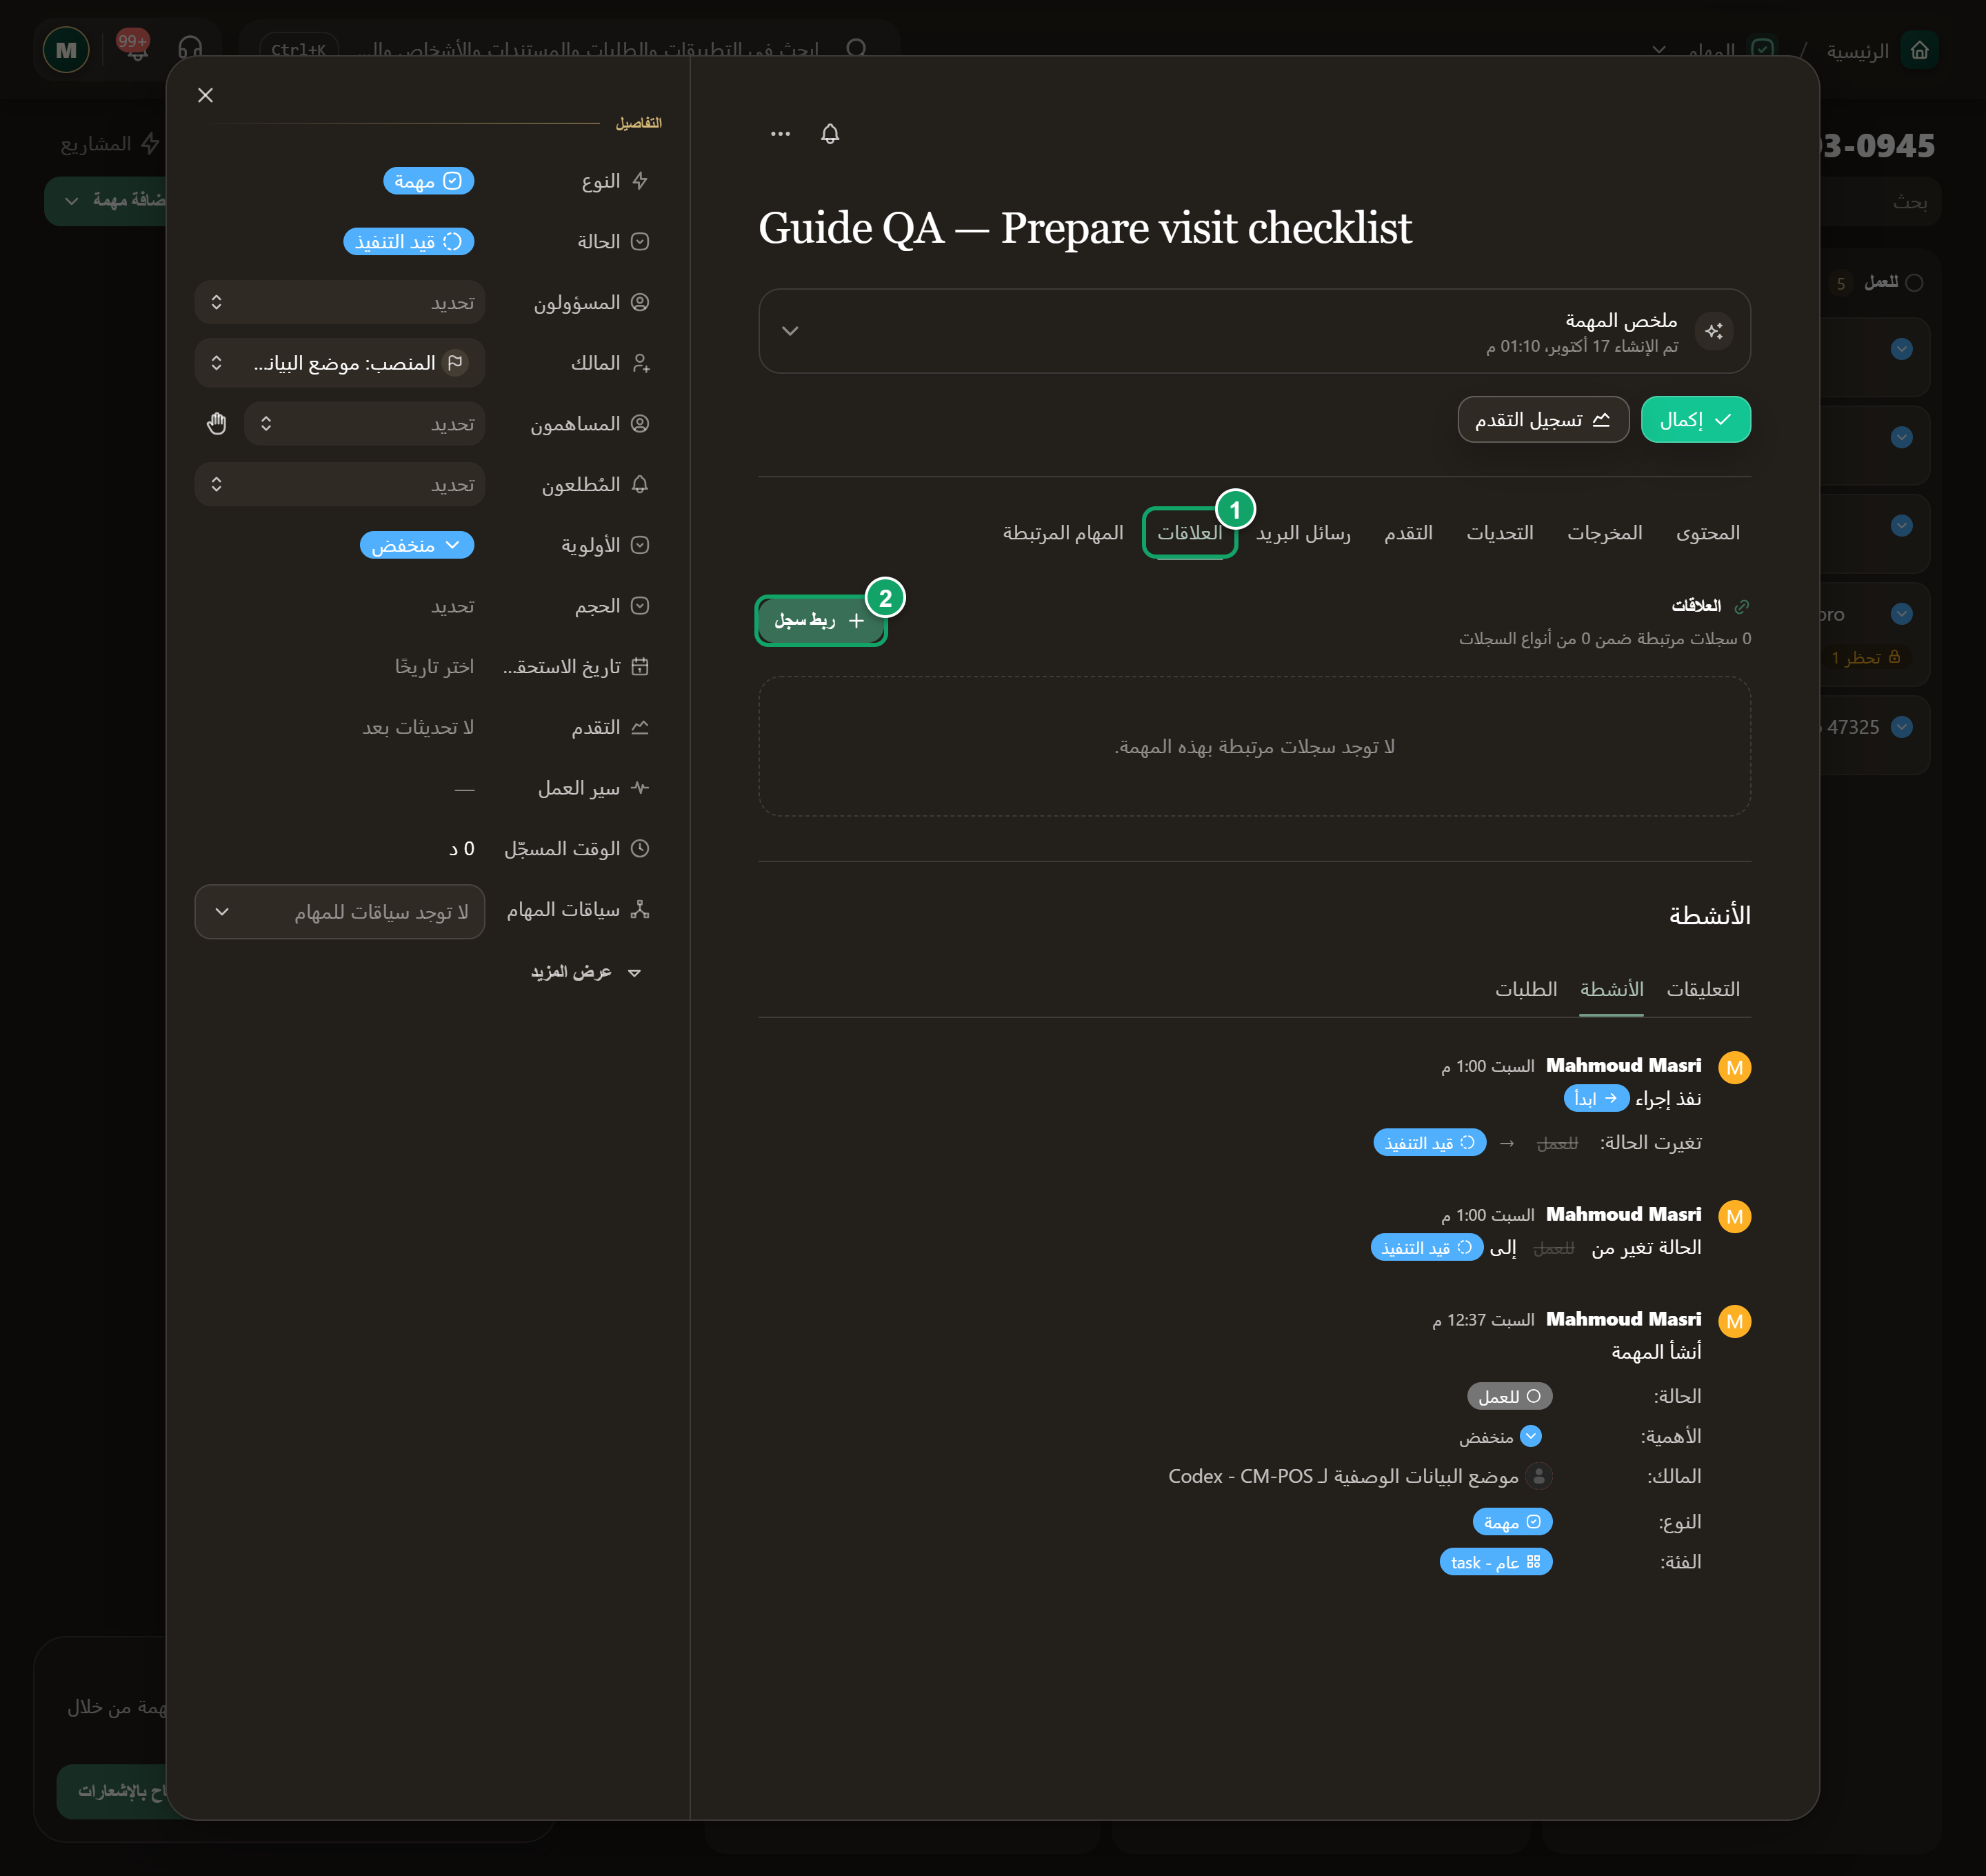
\includegraphics[width=0.95\linewidth,height=0.72\textheight,keepaspectratio]{figures/screens/ch04-records-ar.png}
\caption{علاقات السجلات}
\label{fig:tasks-relationships-records}
\shotnote{يربط تبويب «العلاقات» المهمة بسجلات من خارج المهام، كسجل يمثل موضوعها أو يثبت إنجازها، ويعرض عدد السجلات المرتبطة. ويبدأ الربط بزر «ربط سجل» واختيار معنى العلاقة من الأنواع المسموحة. ولا يمنح الرابط صلاحية فتح السجل لمن لا يملكها، والقائمة فارغة في هذه المهمة التجريبية. ① تبويب «العلاقات». ② «ربط سجل»: يربط المهمة بسجل آخر في كيان.}
\end{figure}

\begin{figure}[H]
\centering
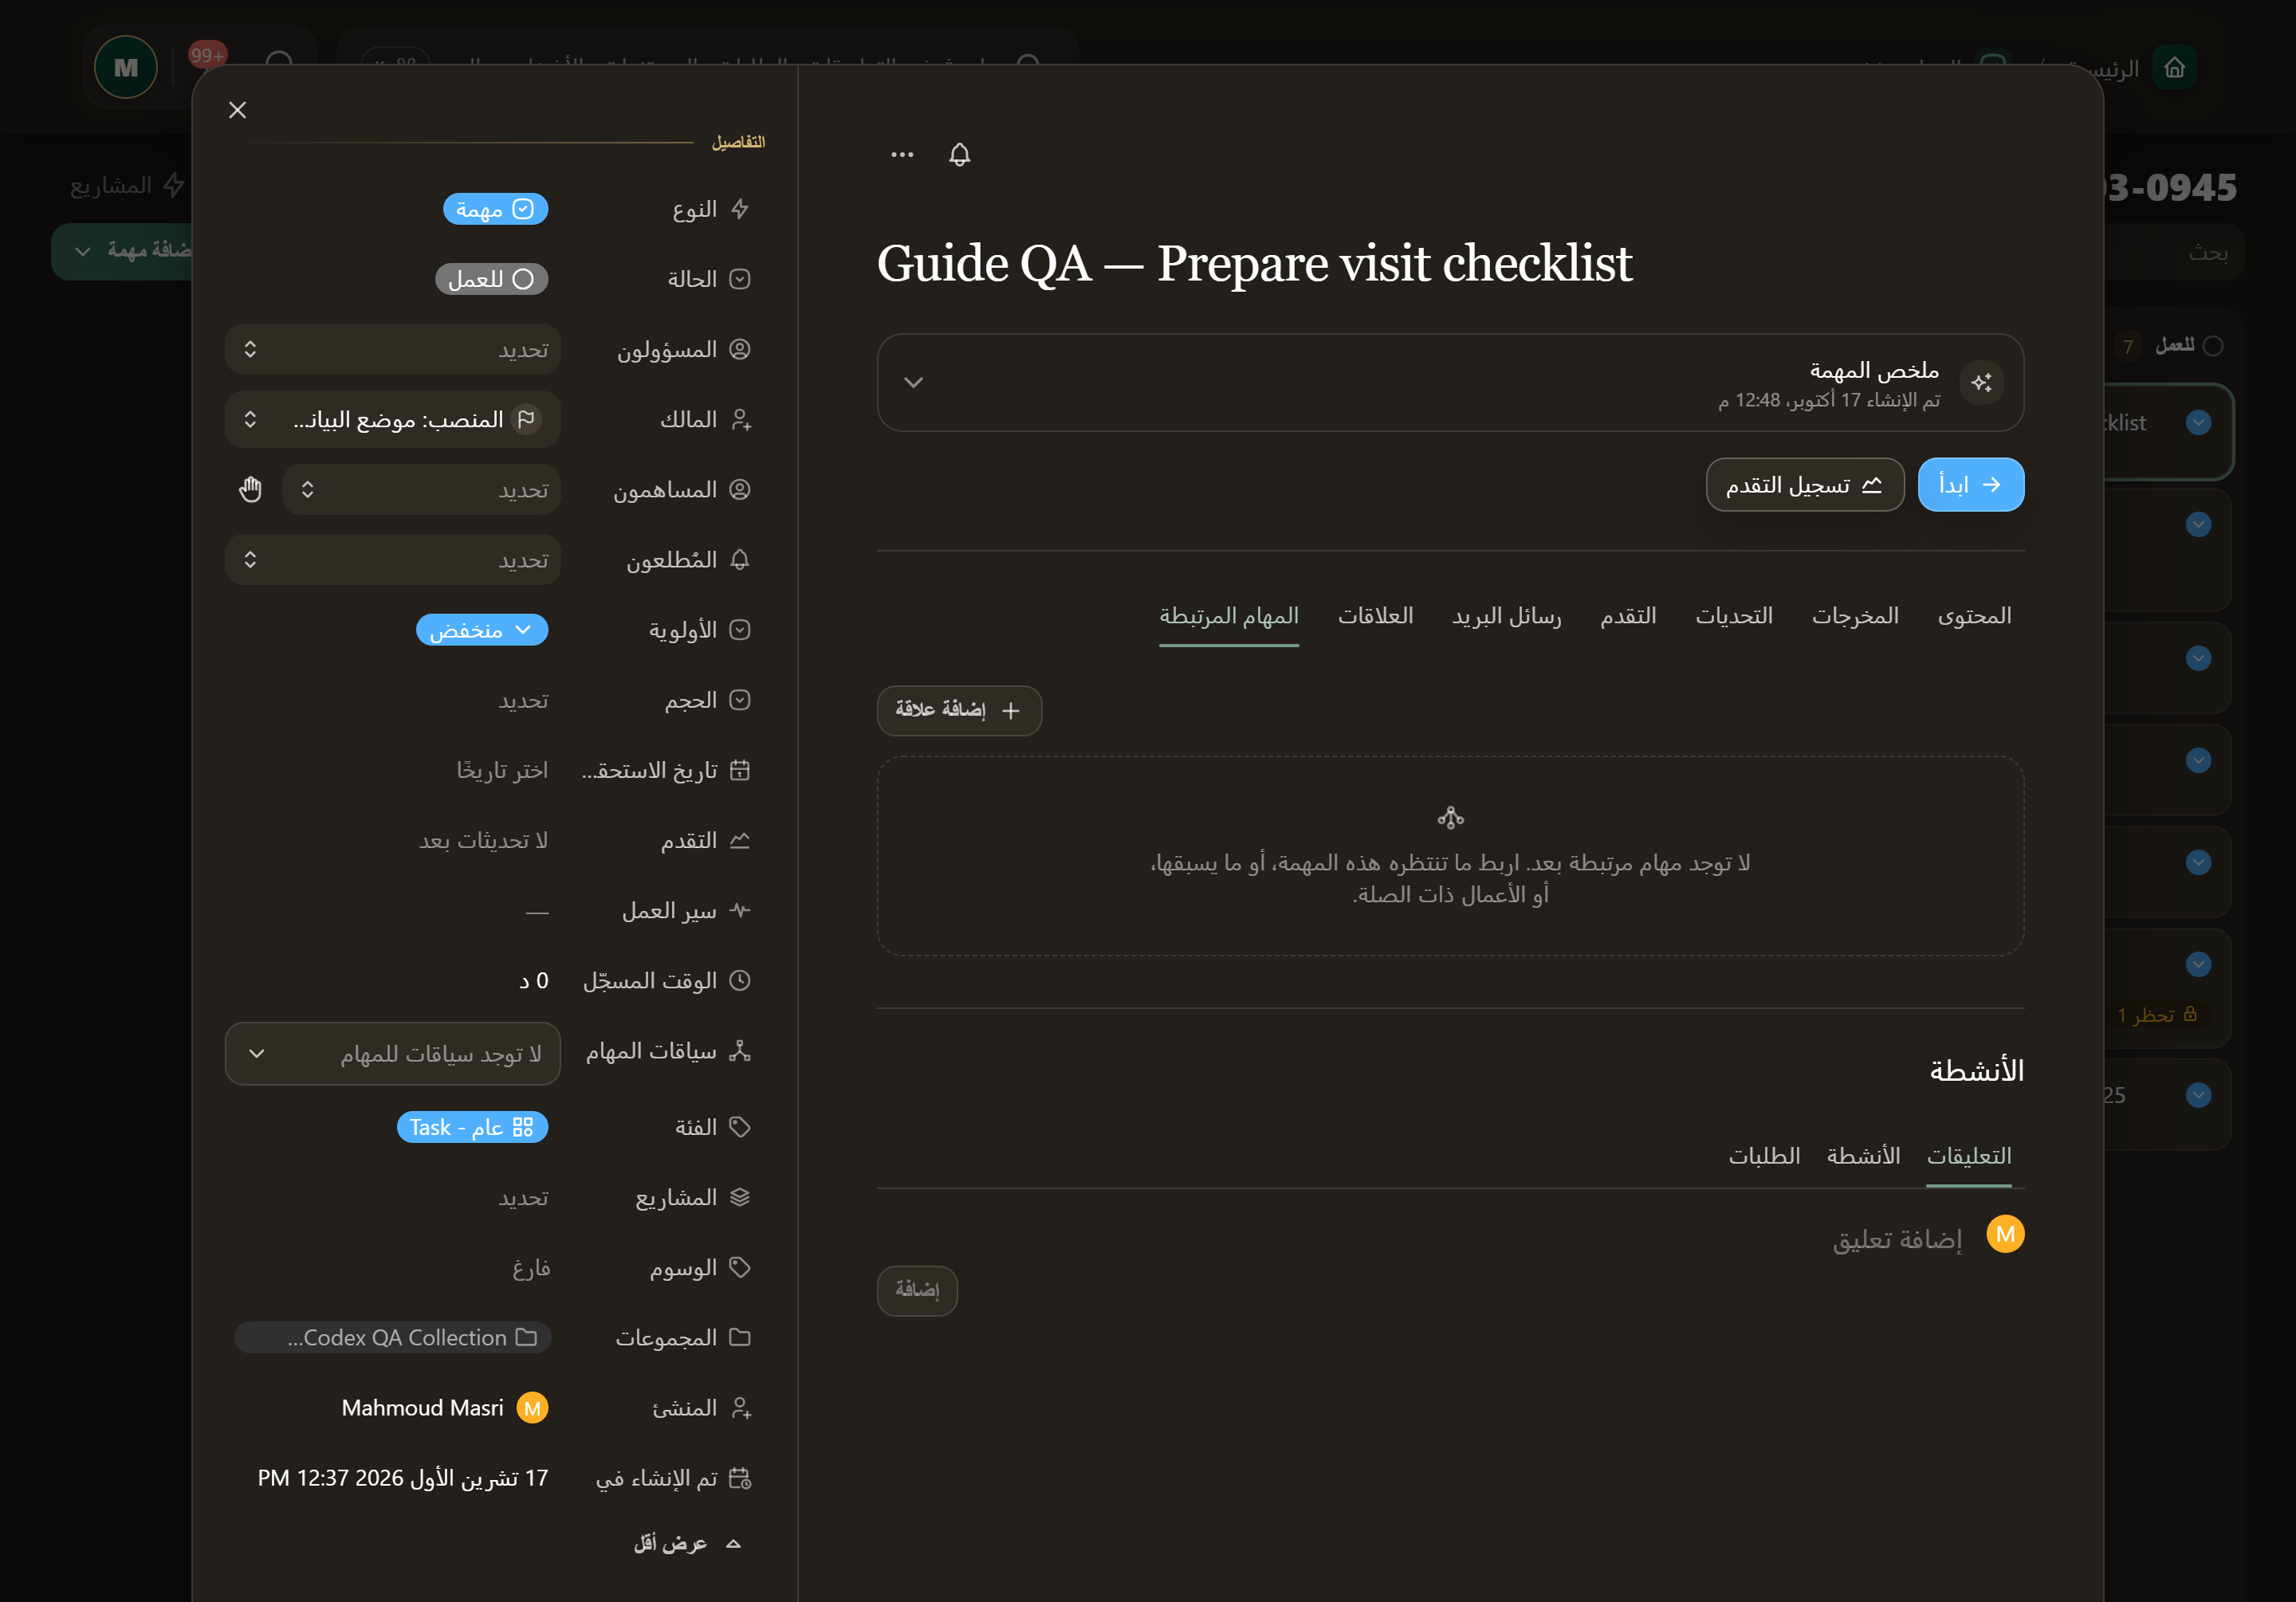
\includegraphics[width=0.95\linewidth,height=0.72\textheight,keepaspectratio]{figures/screens/ch04-relations-ar.png}
\caption{المهام المرتبطة}
\label{fig:tasks-relationships-relations}
\shotnote{يعرض تبويب «المهام المرتبطة» صلة المهمة بمهام أخرى: ما تنتظره، وما يسبقها، وما يتصل بها، ويُضاف الرابط من «إضافة علاقة». وتؤثر بعض هذه العلاقات في ترتيب العمل، لذلك تحقق من اتجاه علاقة الحجب قبل حفظها. ولا توجد علاقات بعد في هذه المهمة التجريبية. ① تبويب «المهام المرتبطة». ② «إضافة علاقة»: يربط المهمة بمهمة أخرى، مثل مهمة تحظرها.}
\end{figure}

\begin{figure}[H]
\centering
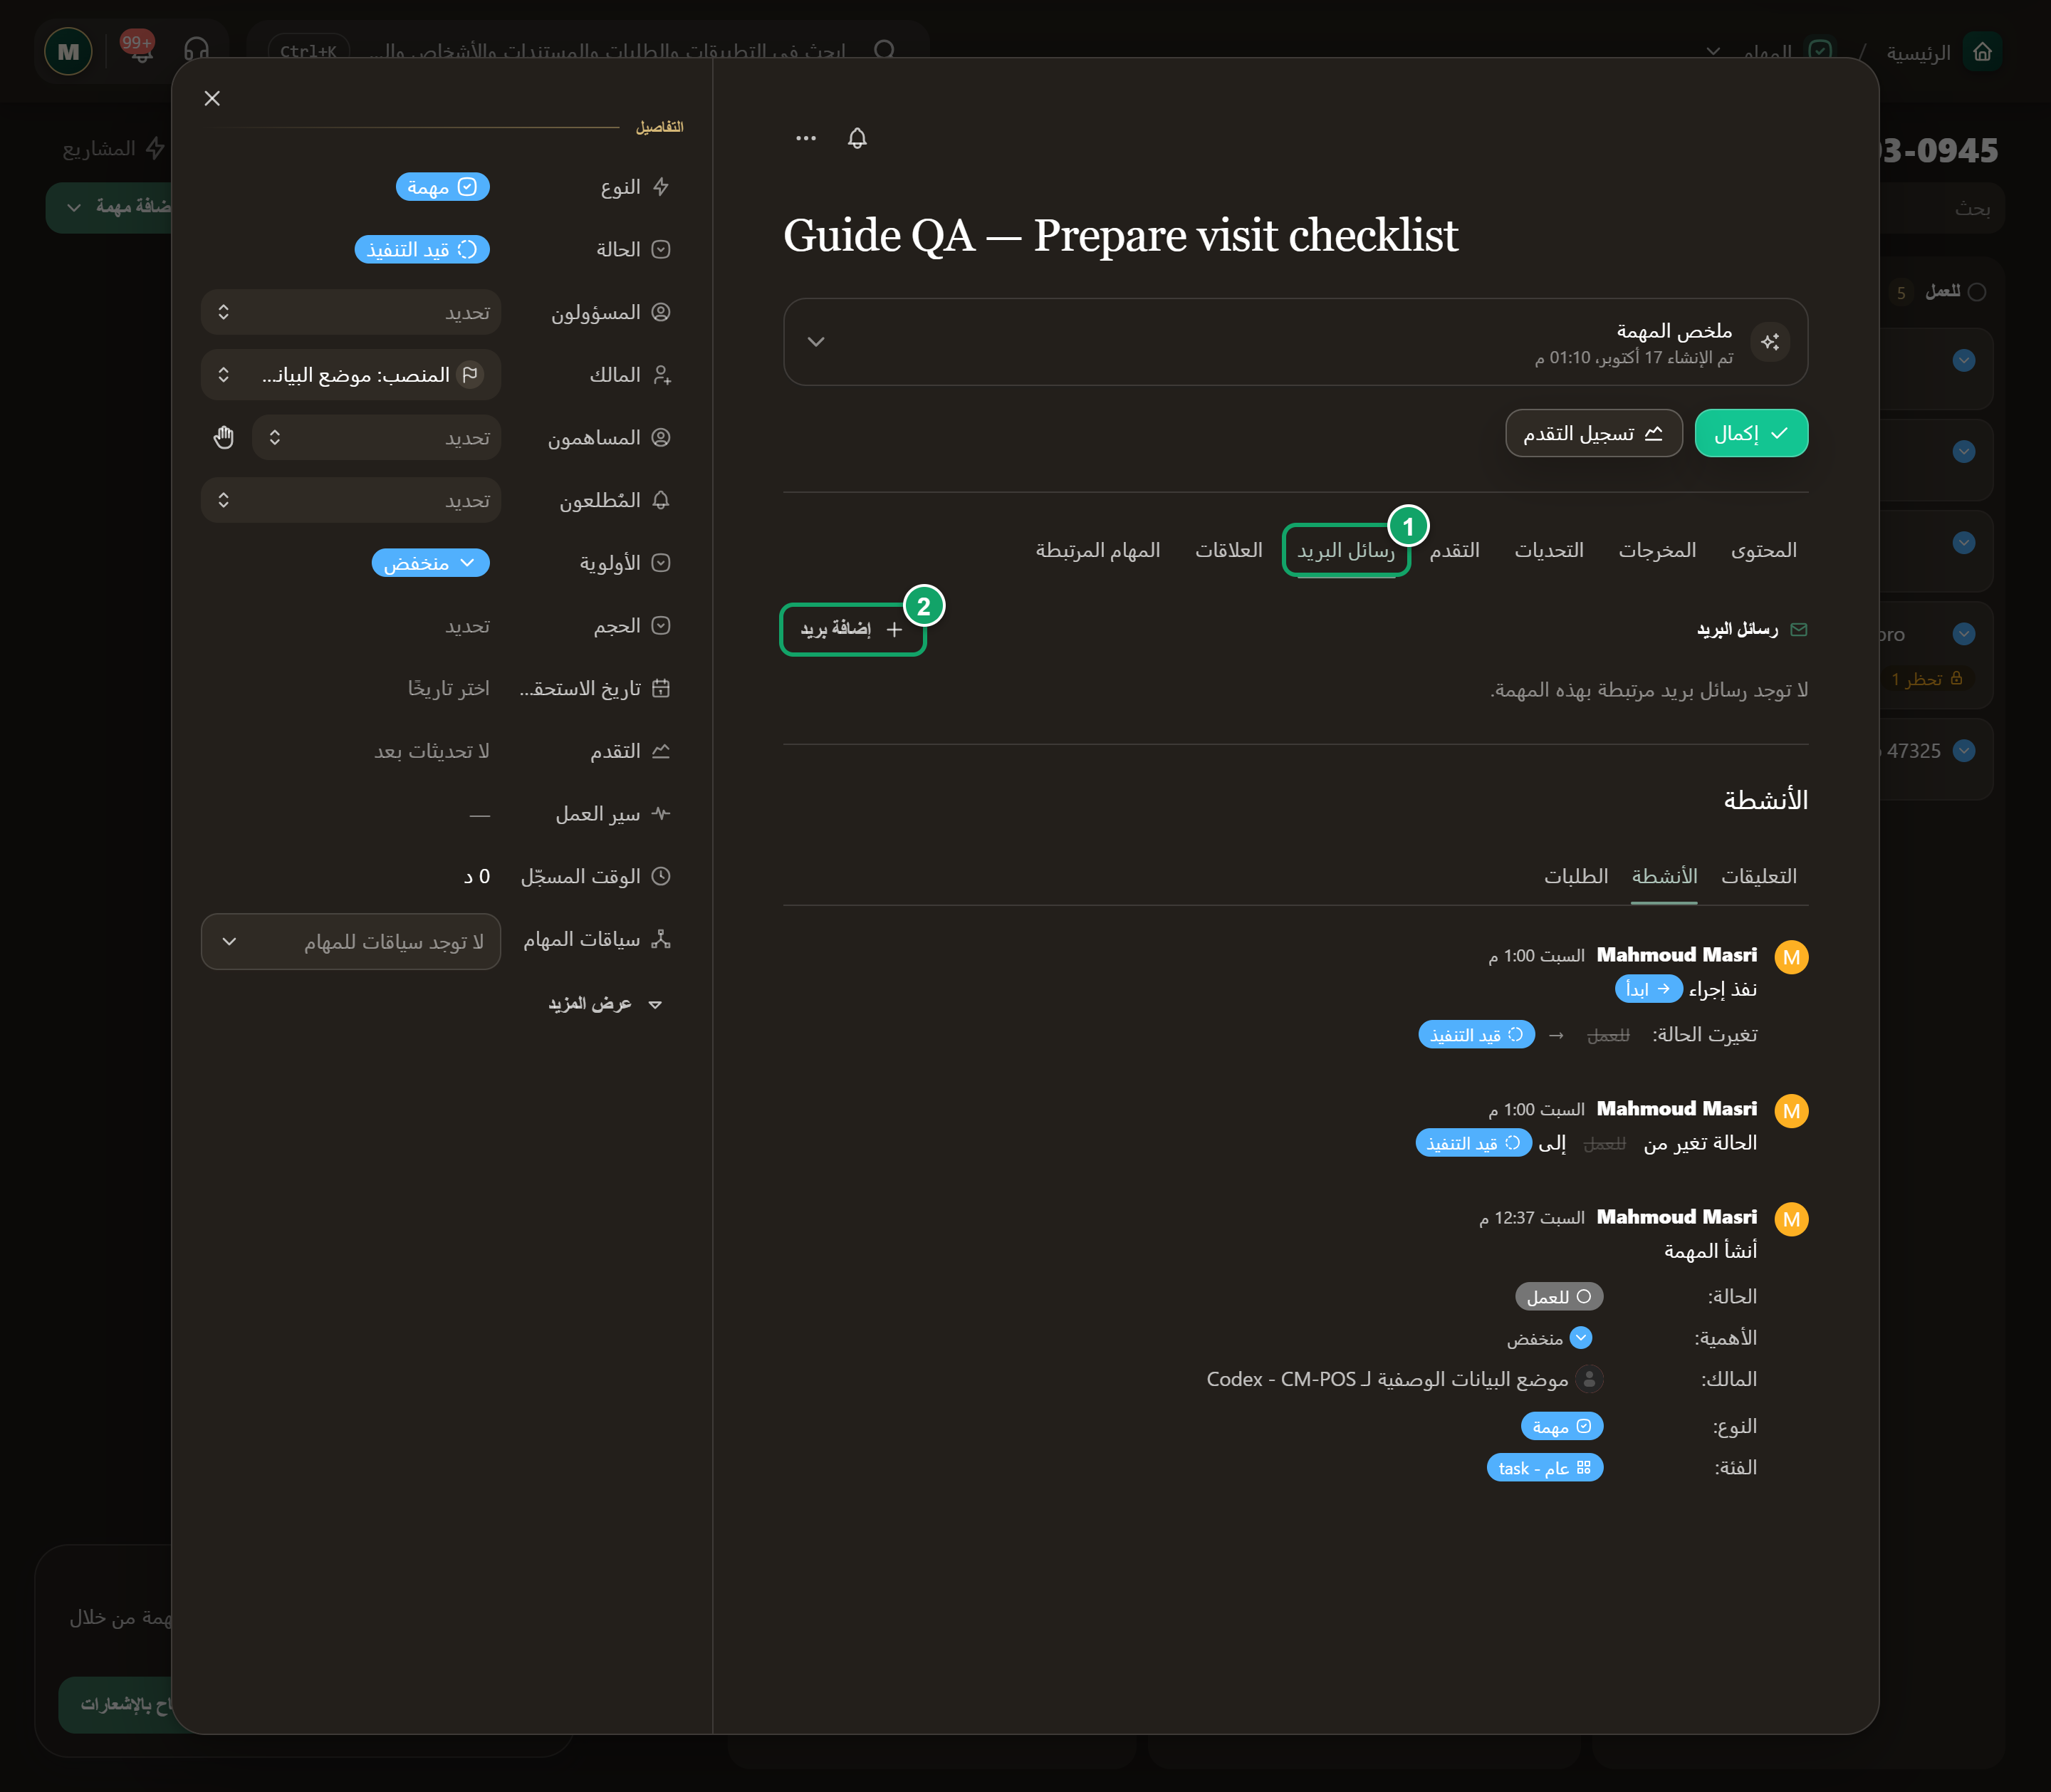
\includegraphics[width=0.95\linewidth,height=0.72\textheight,keepaspectratio]{figures/screens/ch04-emails-ar.png}
\caption{البريد المرتبط}
\label{fig:tasks-relationships-emails}
\shotnote{يجمع تبويب «رسائل البريد» المراسلات المرتبطة بالمهمة، ويربط زر «إضافة بريد» رسالة جديدة بها، فيجد الفريق سياق الطلب الأصلي دون البحث في البريد. والقائمة فارغة هنا، فلا تفترض أن رسالة ما مرتبطة بالمهمة ما لم تظهر في هذا التبويب. ① تبويب «رسائل البريد». ② «إضافة بريد»: يربط رسالة بريد بالمهمة.}
\end{figure}

\begin{table}[H]
\centering
\caption{ما الذي تجده هنا؟}
\label{tab:tasks-relationships-data}
\begin{tabularx}{\linewidth}{R{3.6cm} Y}
\rcHeaderRow
\thh{القسم} & \thh{المحتوى والإجراء}\\
العلاقات & معنى الرابط ونوع السجل والسجل نفسه، مع ملاحظة عند الحاجة. وقد يشترط نوع المهمة روابط معينة عند الإنشاء أو الإكمال.\\
المهام المرتبطة & علاقات بين مهمتين، مثل الحجب أو المهمة الرئيسية والفرعية، بحسب الأنواع المفعّلة. ويمكن البحث في مجموعات أخرى متاحة لك.\\
البريد والسياقات & يقدّم البريد سياق المراسلة، وتربط سياقات المشاريع والتخطيط التنفيذ بالعمل الأكبر، بحسب الخيارات المتاحة.\\
\end{tabularx}
\end{table}

\begin{figure}[H]
\centering
\begin{tikzpicture}[node distance=0.5cm]
\node[stepBox] (a) {\RL{تحديد معنى العلاقة}};
\node[stepBox,below=of a] (b) {\RL{اختيار السجل أو المهمة}};
\node[stepBox,below=of b] (c) {\RL{تحقق من الرابط والاتجاه}};
\draw[flowsTo] (a) -- (b);
\draw[flowsTo] (b) -- (c);
\end{tikzpicture}
\rclegend
\caption{خطوات الاستخدام}
\label{fig:tasks-relationships-flow}
\shotnote{يبدأ الربط الصحيح من المعنى لا من السجل: حدّد أولاً هل الرابط مصدر أو دليل أو تبعية، ثم ابحث عن السجل أو المهمة المناسبة، وتحقق أخيراً من الهدف والاتجاه. فالعلاقة المعكوسة قد تجعل المهمة الخطأ هي التي تنتظر غيرها.}
\end{figure}

\subsection{خطوات العمل والتحقق}
\begin{enumerate}
\item في «العلاقات» اضغط «ربط سجل»، ثم اختر معنى العلاقة ونوع السجل، وابحث عن السجل الصحيح وحدده واحفظ.
\item في «المهام المرتبطة» اضغط «إضافة علاقة»، وحدد النوع والمهمة، وراجع اتجاه العلاقة قبل تأكيدها.
\item افتح الرابط المحفوظ وتأكد أنه يشير إلى السجل المقصود، وراجع المهام الحاجبة قبل محاولة الإكمال.
\end{enumerate}

\textbf{تحقق ومعالجة المشكلة:} إذا لم يظهر السجل، فراجع النوع ونص البحث والصلاحيات. ولا تحذف تبعية صحيحة لتتجاوز منع الإكمال، ولا تعدّ الرابط موافقة أو تحديثاً تلقائياً للسجل.

\clearpage
\section{المهام الكبرى}
\label{sec:tasks-feature-epics}

تجمع المهمة الكبرى عدة مهام تخدم نتيجة أوسع. ويظهر تبويبها في الواجهة العربية باسم «المشاريع»، وهو غير تطبيق المشاريع والتخطيط. استخدمها عندما يحتاج العمل إلى تقسيم مع بقاء الهدف واضحاً في مكان واحد.

\textbf{المسار ومن يستخدمه:} «المهام» ← مجموعة ← تبويب «المشاريع». يستخدمها المسؤول عن مجموعة من الأعمال المترابطة.

\begin{rcnote}[مثال: شركة الأفق]
تنظّم سارة «تجهيز زيارة فرع حلب» مهمةً كبرى، وتربط بها مهمة عمر لتجهيز القائمة ومهمة أخرى لتأكيد الموعد.
\end{rcnote}

\begin{figure}[H]
\centering
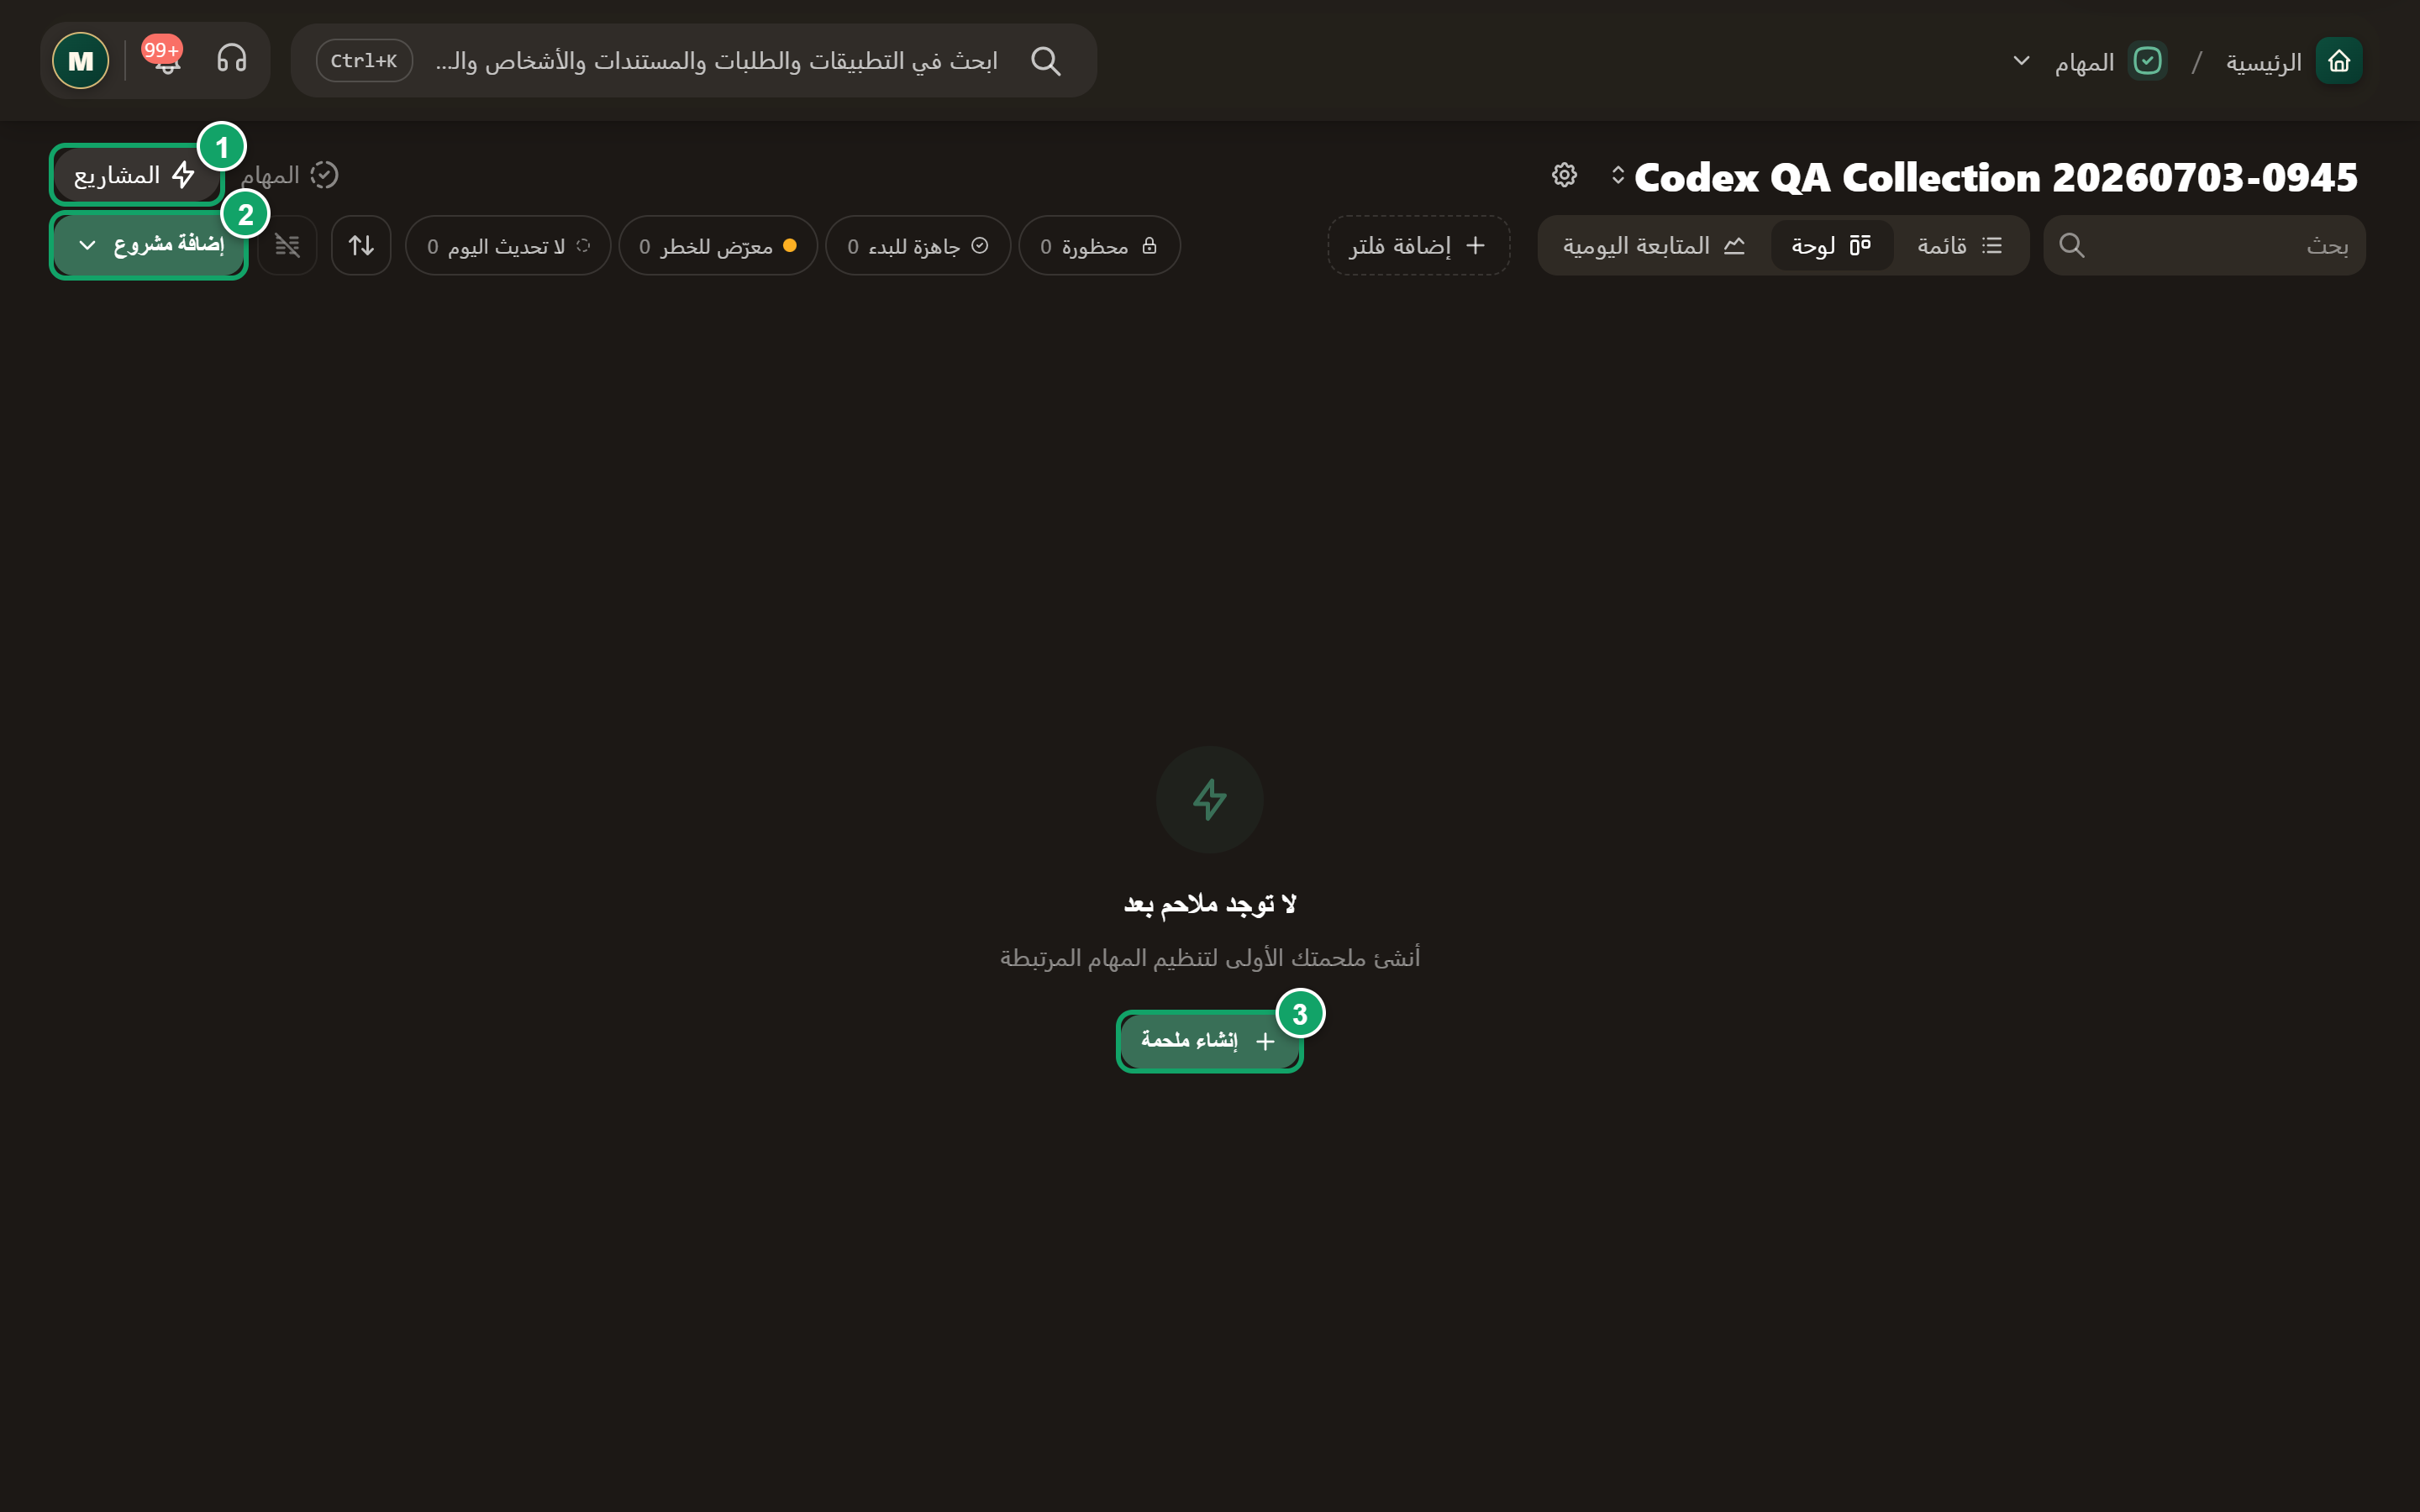
\includegraphics[width=0.95\linewidth,height=0.72\textheight,keepaspectratio]{figures/screens/ch04-epics-ar.png}
\caption{تبويب المهام الكبرى}
\label{fig:tasks-epics-epics}
\shotnote{يعرض تبويب «المشاريع» داخل المجموعة المهام الكبرى بأدوات العرض نفسها التي تستخدمها مع المهام، ويضيف زر «إضافة مشروع». والتبويب فارغ في مجموعة الاختبار، وتسمي رسالته المهمة الكبرى «ملحمة»، وهي تسمية أخرى للشيء نفسه. ولا يفتح هذا التبويب تطبيق المشاريع والتخطيط. ① التبديل إلى عرض «المشاريع»، أي المهام الكبرى في المجموعة. ② «إضافة مشروع»: ينشئ مهمة كبرى جديدة. ③ «إنشاء ملحمة»: يفعل الشيء نفسه عندما لا توجد مهام كبرى بعد.}
\end{figure}

\begin{table}[H]
\centering
\caption{ما الذي تجده هنا؟}
\label{tab:tasks-epics-data}
\begin{tabularx}{\linewidth}{R{3.6cm} Y}
\rcHeaderRow
\thh{القسم} & \thh{المحتوى والإجراء}\\
التفاصيل والمحتوى & العنوان والنوع والحالة والمسؤوليات والموعد والمحتوى، بحسب نوع المهمة الكبرى.\\
المهام التابعة & إنشاء مهمة أو ربط مهمة موجودة، وفتحها أو إزالة ربطها بحسب الصلاحية. وإزالة الربط لا تحذف المهمة.\\
\end{tabularx}
\end{table}

\begin{figure}[H]
\centering
\begin{tikzpicture}[node distance=0.5cm]
\node[stepBox] (a) {\RL{تحديد النتيجة العامة}};
\node[stepBox,below=of a] (b) {\RL{ربط المهام}};
\node[stepBox,below=of b] (c) {\RL{متابعة كل نتيجة}};
\draw[flowsTo] (a) -- (b);
\draw[flowsTo] (b) -- (c);
\end{tikzpicture}
\rclegend
\caption{خطوات الاستخدام}
\label{fig:tasks-epics-flow}
\shotnote{يبيّن المخطط أن المهمة الكبرى إطار للمتابعة لا بديل عن المهام: حدّد النتيجة العامة، ثم اربط بها المهام التي تحققها، وتابع نتيجة كل مهمة على حدة. وبذلك تقيّم العمل كله من نتائج أجزائه، لا من حالة المهمة الكبرى وحدها.}
\end{figure}

\subsection{خطوات العمل والتحقق}
\begin{enumerate}
\item افتح تبويب «المشاريع»، واضغط «إضافة مشروع» واختر النوع المتاح، ثم اكتب النتيجة العامة والمسؤولية وأنشئ السجل.
\item داخل المهمة الكبرى أضف مهمة أو اربط مهمة موجودة، واختر عنوان العمل الصحيح ثم أكّد الربط.
\item افتح المهمة التابعة وتحقق من الربط، وتابع حالة كل مهمة قبل تحديث المهمة الكبرى.
\end{enumerate}

\textbf{تحقق ومعالجة المشكلة:} لا تفترض أن إغلاق المهمة الكبرى يغلق المهام التابعة أو أي مشروع مرتبط، بل راجع النتائج والحالات كلاً على حدة.

\clearpage
\section{اقتراحات الذكاء الاصطناعي}
\label{sec:tasks-feature-suggestions}

المقترح عمل مستخرج من رسائل البريد، ويحتاج إلى مراجعة قبل أن يصبح مهمة فعلية. راجع مصدره والمسؤولية والموعد قبل قبوله.

\textbf{المسار ومن يستخدمه:} «المهام» ← بطاقة «اقتراحات الذكاء الاصطناعي» عند تفعيلها. يستخدمها المراجع المخوّل.

\begin{rcnote}[مثال: شركة الأفق]
تراجع سارة مقترحاً لتأكيد زيارة الأفق، فتختار مجموعة «زيارات الأفق» عند القبول، ثم تصحح الموعد في المهمة الناتجة.
\end{rcnote}

\begin{figure}[H]
\centering
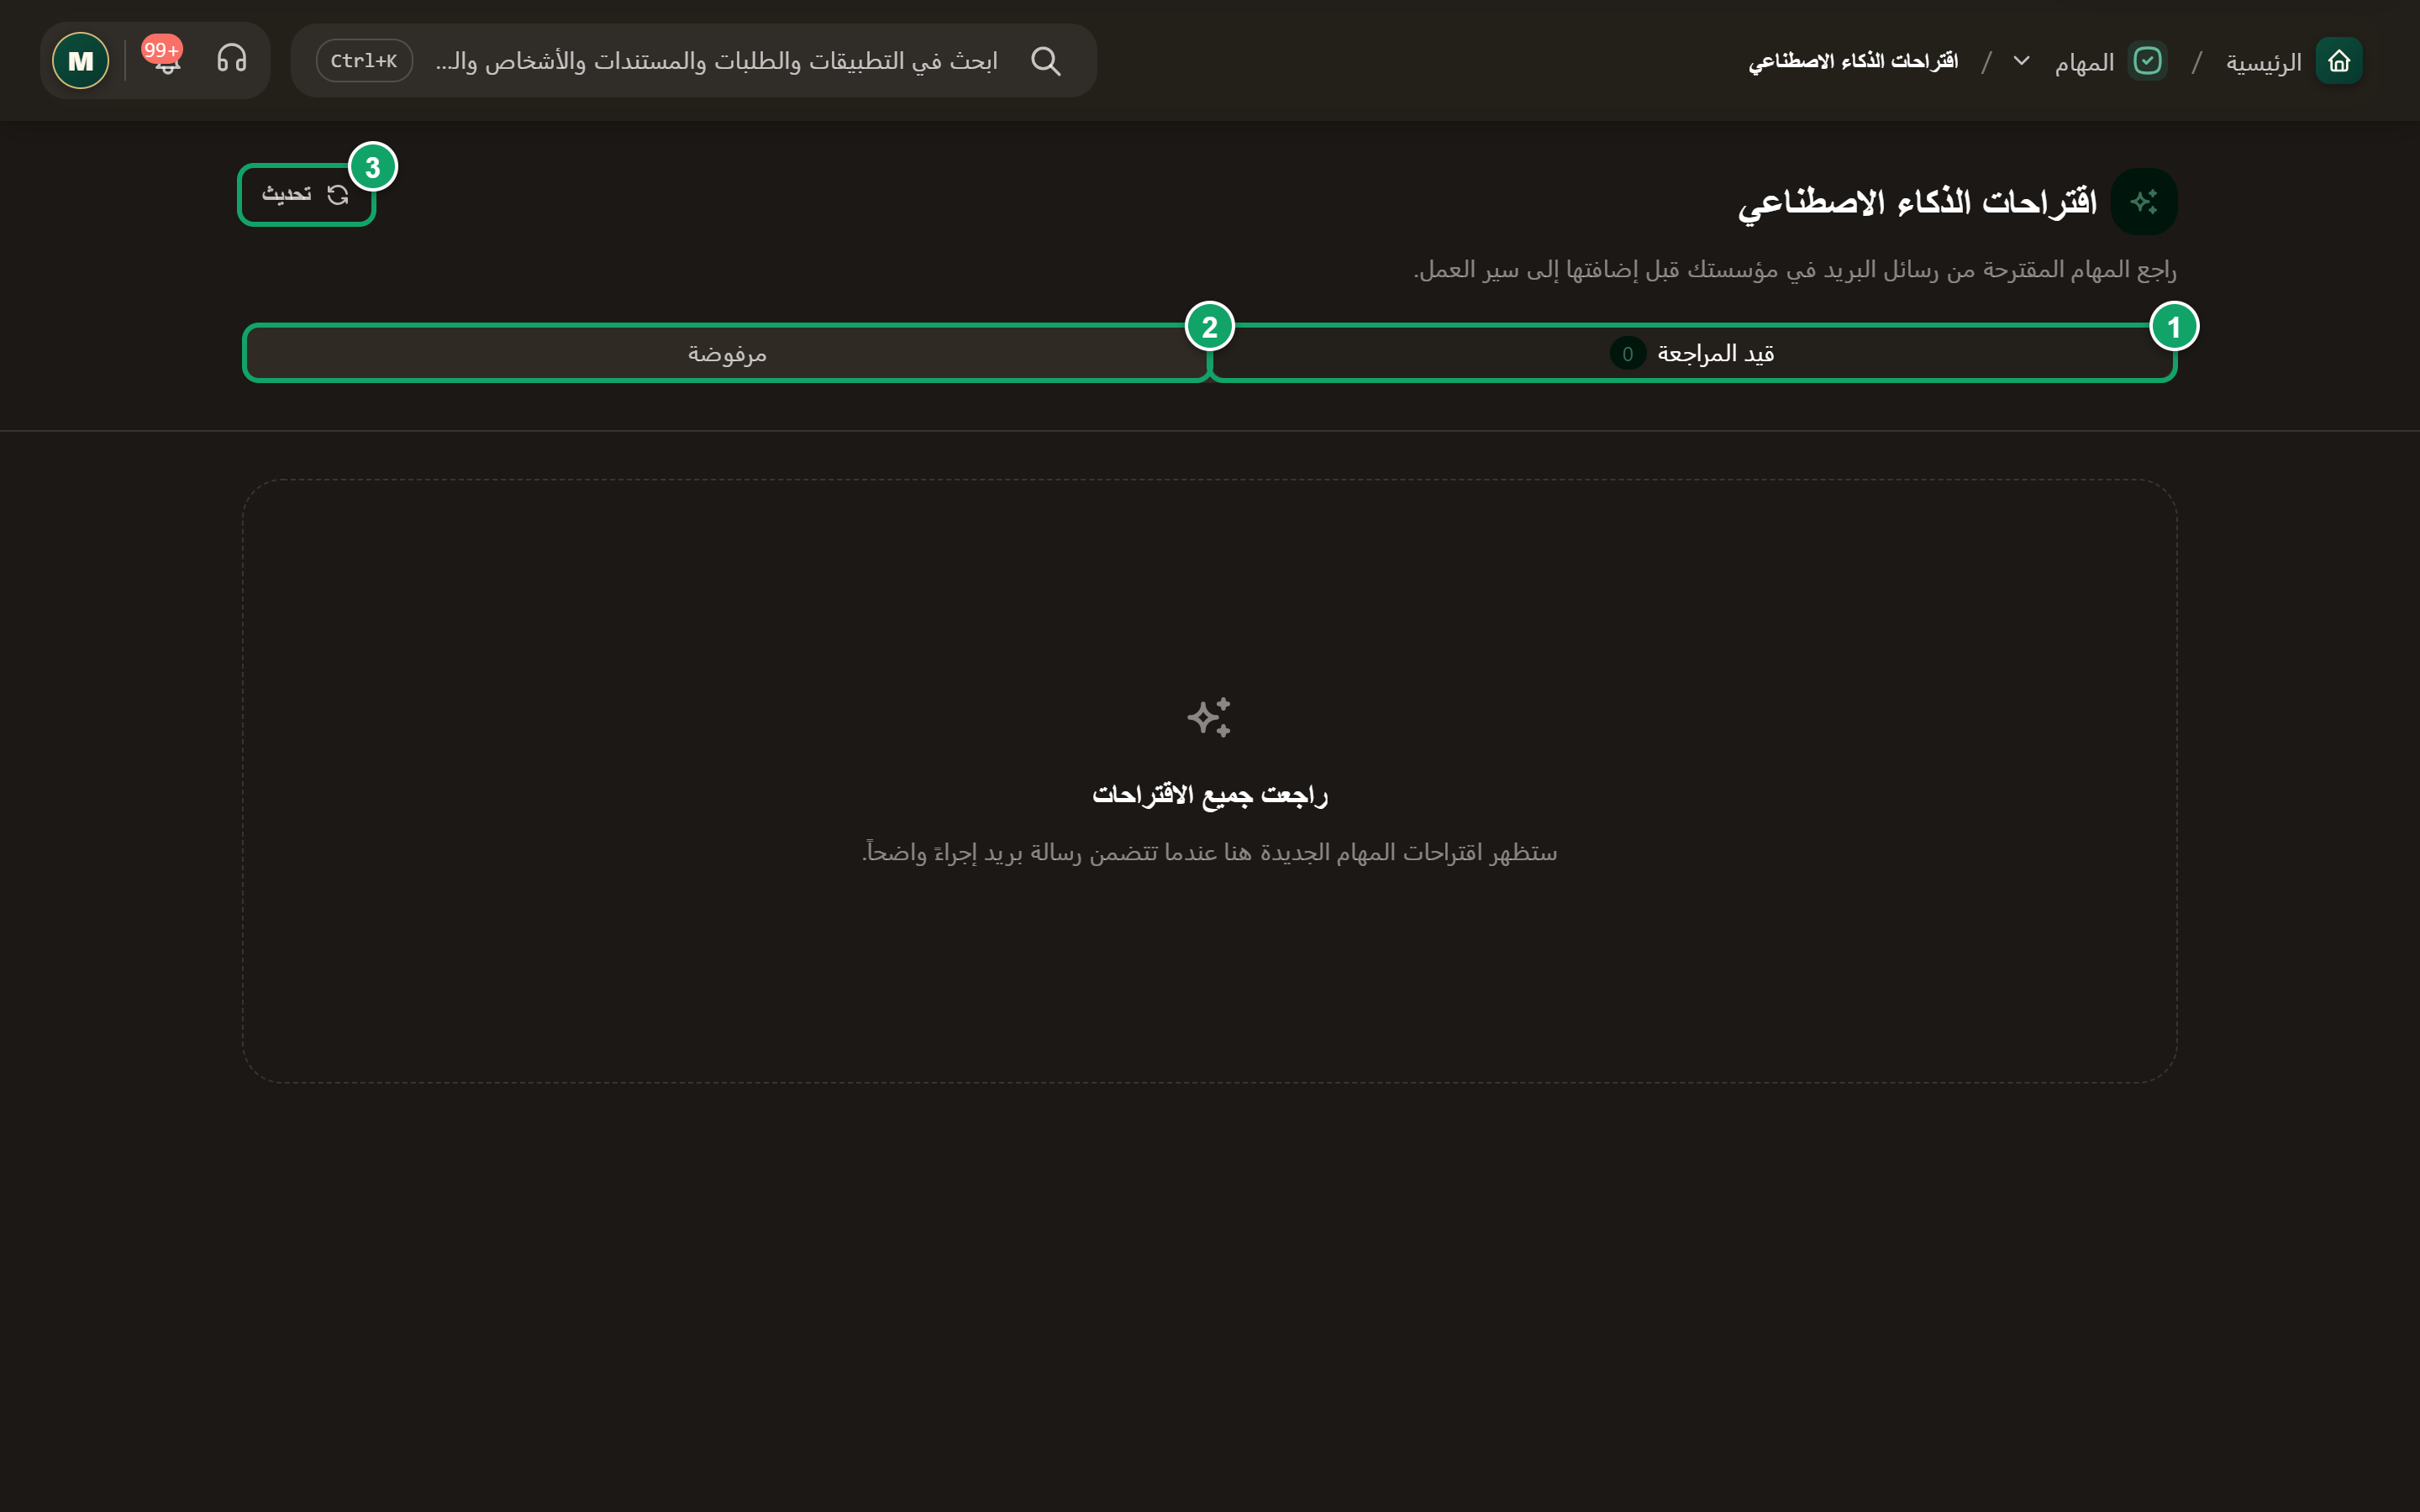
\includegraphics[width=0.95\linewidth,height=0.72\textheight,keepaspectratio]{figures/screens/ch04-suggestions-ar.png}
\caption{قائمة المقترحات}
\label{fig:tasks-suggestions-suggestions}
\shotnote{تجمع هذه الصفحة المهام المقترحة من رسائل البريد في تبويبين: «قيد المراجعة» لما ينتظر قرارك، و«مرفوضة» لما استبعدته، فلا يدخل المقترح سير العمل حتى يقبله مراجع. والقائمة فارغة في test2 وقت الالتقاط، لذلك لم يُختبر القبول هنا. ① «قيد المراجعة»: الاقتراحات التي تنتظر قرارك. ② «مرفوضة». ③ «تحديث».}
\end{figure}

\begin{table}[H]
\centering
\caption{ما الذي تجده هنا؟}
\label{tab:tasks-suggestions-data}
\begin{tabularx}{\linewidth}{R{3.6cm} Y}
\rcHeaderRow
\thh{القسم} & \thh{المحتوى والإجراء}\\
الحالة والمصدر & صفِّ المقترحات بحالتها، وافتح تفاصيلها، وراجع البريد الذي استندت إليه.\\
القبول أو الرفض & يتطلب القبول مجموعة ونوعاً مسموحين وبيانات صحيحة، أما الرفض فلا يعني إكمال مهمة.\\
\end{tabularx}
\end{table}

\begin{figure}[H]
\centering
\begin{tikzpicture}[node distance=0.5cm]
\node[stepBox] (a) {\RL{قراءة المصدر}};
\node[stepBox,below=of a] (b) {\RL{مراجعة المقترح}};
\node[stepBox,below=of b] (c) {\RL{قبول ثم تحقق}};
\draw[flowsTo] (a) -- (b);
\draw[flowsTo] (b) -- (c);
\end{tikzpicture}
\rclegend
\caption{خطوات الاستخدام}
\label{fig:tasks-suggestions-flow}
\shotnote{يضع المخطط قراءة المصدر قبل أي قرار، لأن رسالة البريد هي التي تفسر سبب المقترح ومن طلبه. ثم تأتي مراجعة تفاصيله، وبعدها القبول والتحقق من المهمة الناتجة؛ إذ لا يتحول المقترح إلى مهمة إلا بقرار من المراجع.}
\end{figure}

\subsection{خطوات العمل والتحقق}
\begin{enumerate}
\item افتح «اقتراحات الذكاء الاصطناعي» واختر «قيد المراجعة»، ثم افتح مقترحاً إن وُجد واقرأ مصدره.
\item راجع المقترح ومصدره قبل القبول، ثم اختر نوع المهمة ومجموعة واحدة على الأقل وأكّد القبول، أو ارفض المقترح غير المناسب.
\item بعد القبول افتح المهمة الناتجة، وصحّح العنوان والأشخاص والتاريخ عند الحاجة، ثم تحقق من الحفظ. أما إذا كانت القائمة فارغة فلا يوجد ما تقبله.
\end{enumerate}

\textbf{تحقق ومعالجة المشكلة:} إذا غاب النوع المطلوب، فراجع صلاحية إنشائه وقيود المجموعة. وتذكّر أن المقترح وحده ليس تكليفاً مؤكداً.

\clearpage
\section{التكليفات}
\label{sec:tasks-feature-assignments}

تعرض «التكليفات» النماذج المطلوب منك تعبئتها والعمل المرتبط بها، فتبدأ من التكليف وتعود إليه لمراجعة نتيجته. أما تصميم النماذج وإدارة خطط التكليف فلهما أدوات أخرى.

\textbf{المسار ومن يستخدمه:} «المهام» ← «التكليفات». يستخدمها الشخص المكلّف بتعبئة نموذج.

\begin{rcnote}[مثال: شركة الأفق]
يفتح عمر تكليف نموذج زيارة الأفق، فيكمل حقوله ثم يرسله، وتراجع سارة النتيجة وفق مسار النموذج.
\end{rcnote}

\begin{figure}[H]
\centering

\includegraphics[width=0.95\linewidth,height=0.72\textheight,keepaspectratio]{figures/screens/ch04-assignments-ar.png}
\caption{قائمة التكليفات}
\label{fig:tasks-assignments-assignments}
\shotnote{تجمع الصفحة العمل المطلوب منك في «المطلوب مني» وترتبه حسب الموعد، ولكل تكليف زر يناسب حالته لبدء التعبئة أو متابعتها. ويُظهر التبديل بين «مفتوحة» و«منجزة» العمل الحالي أو السابق، أما تبويب «الخطط» فيخص متابعة توزيع العمل. وتظهر بطاقة «عمل اليوم» عندما يتوفر تكليف يمكن تنزيله للعمل دون اتصال. ① عنوان صفحة «التكليفات». ② «المطلوب مني»: النماذج المسندة إليك وعددها.}
\end{figure}

\begin{table}[H]
\centering
\caption{ما الذي تجده هنا؟}
\label{tab:tasks-assignments-data}
\begin{tabularx}{\linewidth}{R{3.6cm} Y}
\rcHeaderRow
\thh{القسم} & \thh{المحتوى والإجراء}\\
بطاقة التكليف & عنوان النموذج والموعد والحالة والنتيجة المتاحة.\\
الإجراءات & البدء أو المتابعة أو العرض، واستلام التكليف أو «اعتذار» حيث تسمح الخطة. وقد يطلب إجراء «نتيجة دون إجابة» سبباً أو صورة أو موقعاً قبل الإغلاق.\\
المطلوب مني والخطط & يعرض «المطلوب مني» تكليفاتك مرتبة حسب الموعد، ويفتح «الخطط» متابعة توزيع العمل لمن يملك صلاحيتها.\\
الحزم والعمل الميداني & تجمع الحزمة نماذج مترابطة وتعرض الوحدة التالية. ويظهر تنزيل العمل دون اتصال و«صندوق الإرسال» للعمل المؤهل، فتحقق من المزامنة عند عودة الاتصال.\\
الغياب والترتيب & يسجّل «غائب حتى…» فترة عدم توفرك، وقد يتاح ترتيب المجموعات أو عرض الخريطة بحسب بيانات العمل.\\
\end{tabularx}
\end{table}

\begin{figure}[H]
\centering
\begin{tikzpicture}[node distance=0.5cm]
\node[stepBox] (a) {\RL{فتح التكليف}};
\node[stepBox,below=of a] (b) {\RL{تعبئة وإرسال}};
\node[stepBox,below=of b] (c) {\RL{مراجعة النتيجة}};
\draw[flowsTo] (a) -- (b);
\draw[flowsTo] (b) -- (c);
\end{tikzpicture}
\rclegend
\caption{خطوات الاستخدام}
\label{fig:tasks-assignments-flow}
\shotnote{يربط المخطط بداية العمل بنهايته: افتح التكليف نفسه لتصل إلى النموذج الصحيح، ثم عبّئه وأرسله، وبعدها راجع نتيجته. فوجود مسودة لا يعني أن التكليف أُنجز؛ العبرة بالإرسال وبالنتيجة التي تظهر بعده.}
\end{figure}

\subsection{خطوات العمل والتحقق}
\begin{enumerate}
\item افتح «التكليفات» واختر التكليف المقصود، وإن كان متاحاً للاستلام فاستلمه قبل البدء.
\item اختر البدء أو المتابعة، وأكمل حقول النموذج، ثم استخدم إجراء الإرسال الذي يقدمه النموذج.
\item ارجع إلى «التكليفات» واعرض «منجزة» عند الحاجة، ثم اضغط «عرض» للتحقق. أما «نتيجة دون إجابة» فإجراء مستقل يغلق التكليف عند السماح به، وليس زراً لعرض النتيجة.
\end{enumerate}

\textbf{تحقق ومعالجة المشكلة:} الحفظ كمسودة ليس إرسالاً. وإذا لم يظهر تكليف متوقع، فراجع المستلم والخطة والصلاحية مع المسؤول.

\clearpage
\section{إعدادات المهام}
\label{sec:tasks-feature-settings}

تحدد إعدادات المهام أنواع العمل وفئاته والعلاقات المتاحة. وهي تهيئة يتولاها المسؤول، أما الموظف فيستخدم عادةً الأنواع الجاهزة.

\textbf{المسار ومن يستخدمه:} «أدوات البناء» ← «إعدادات المهام». يستخدمها المسؤول المخوّل.

\begin{rcnote}[مثال: شركة الأفق]
تراجع سارة مع المسؤول نوع مهمة الزيارة: الفئة الافتراضية، ومسار الحالات، وهل يلزم تحديث التقدم. ثم تستخدم هذا النوع في مهام الأفق.
\end{rcnote}

\begin{figure}[H]
\centering
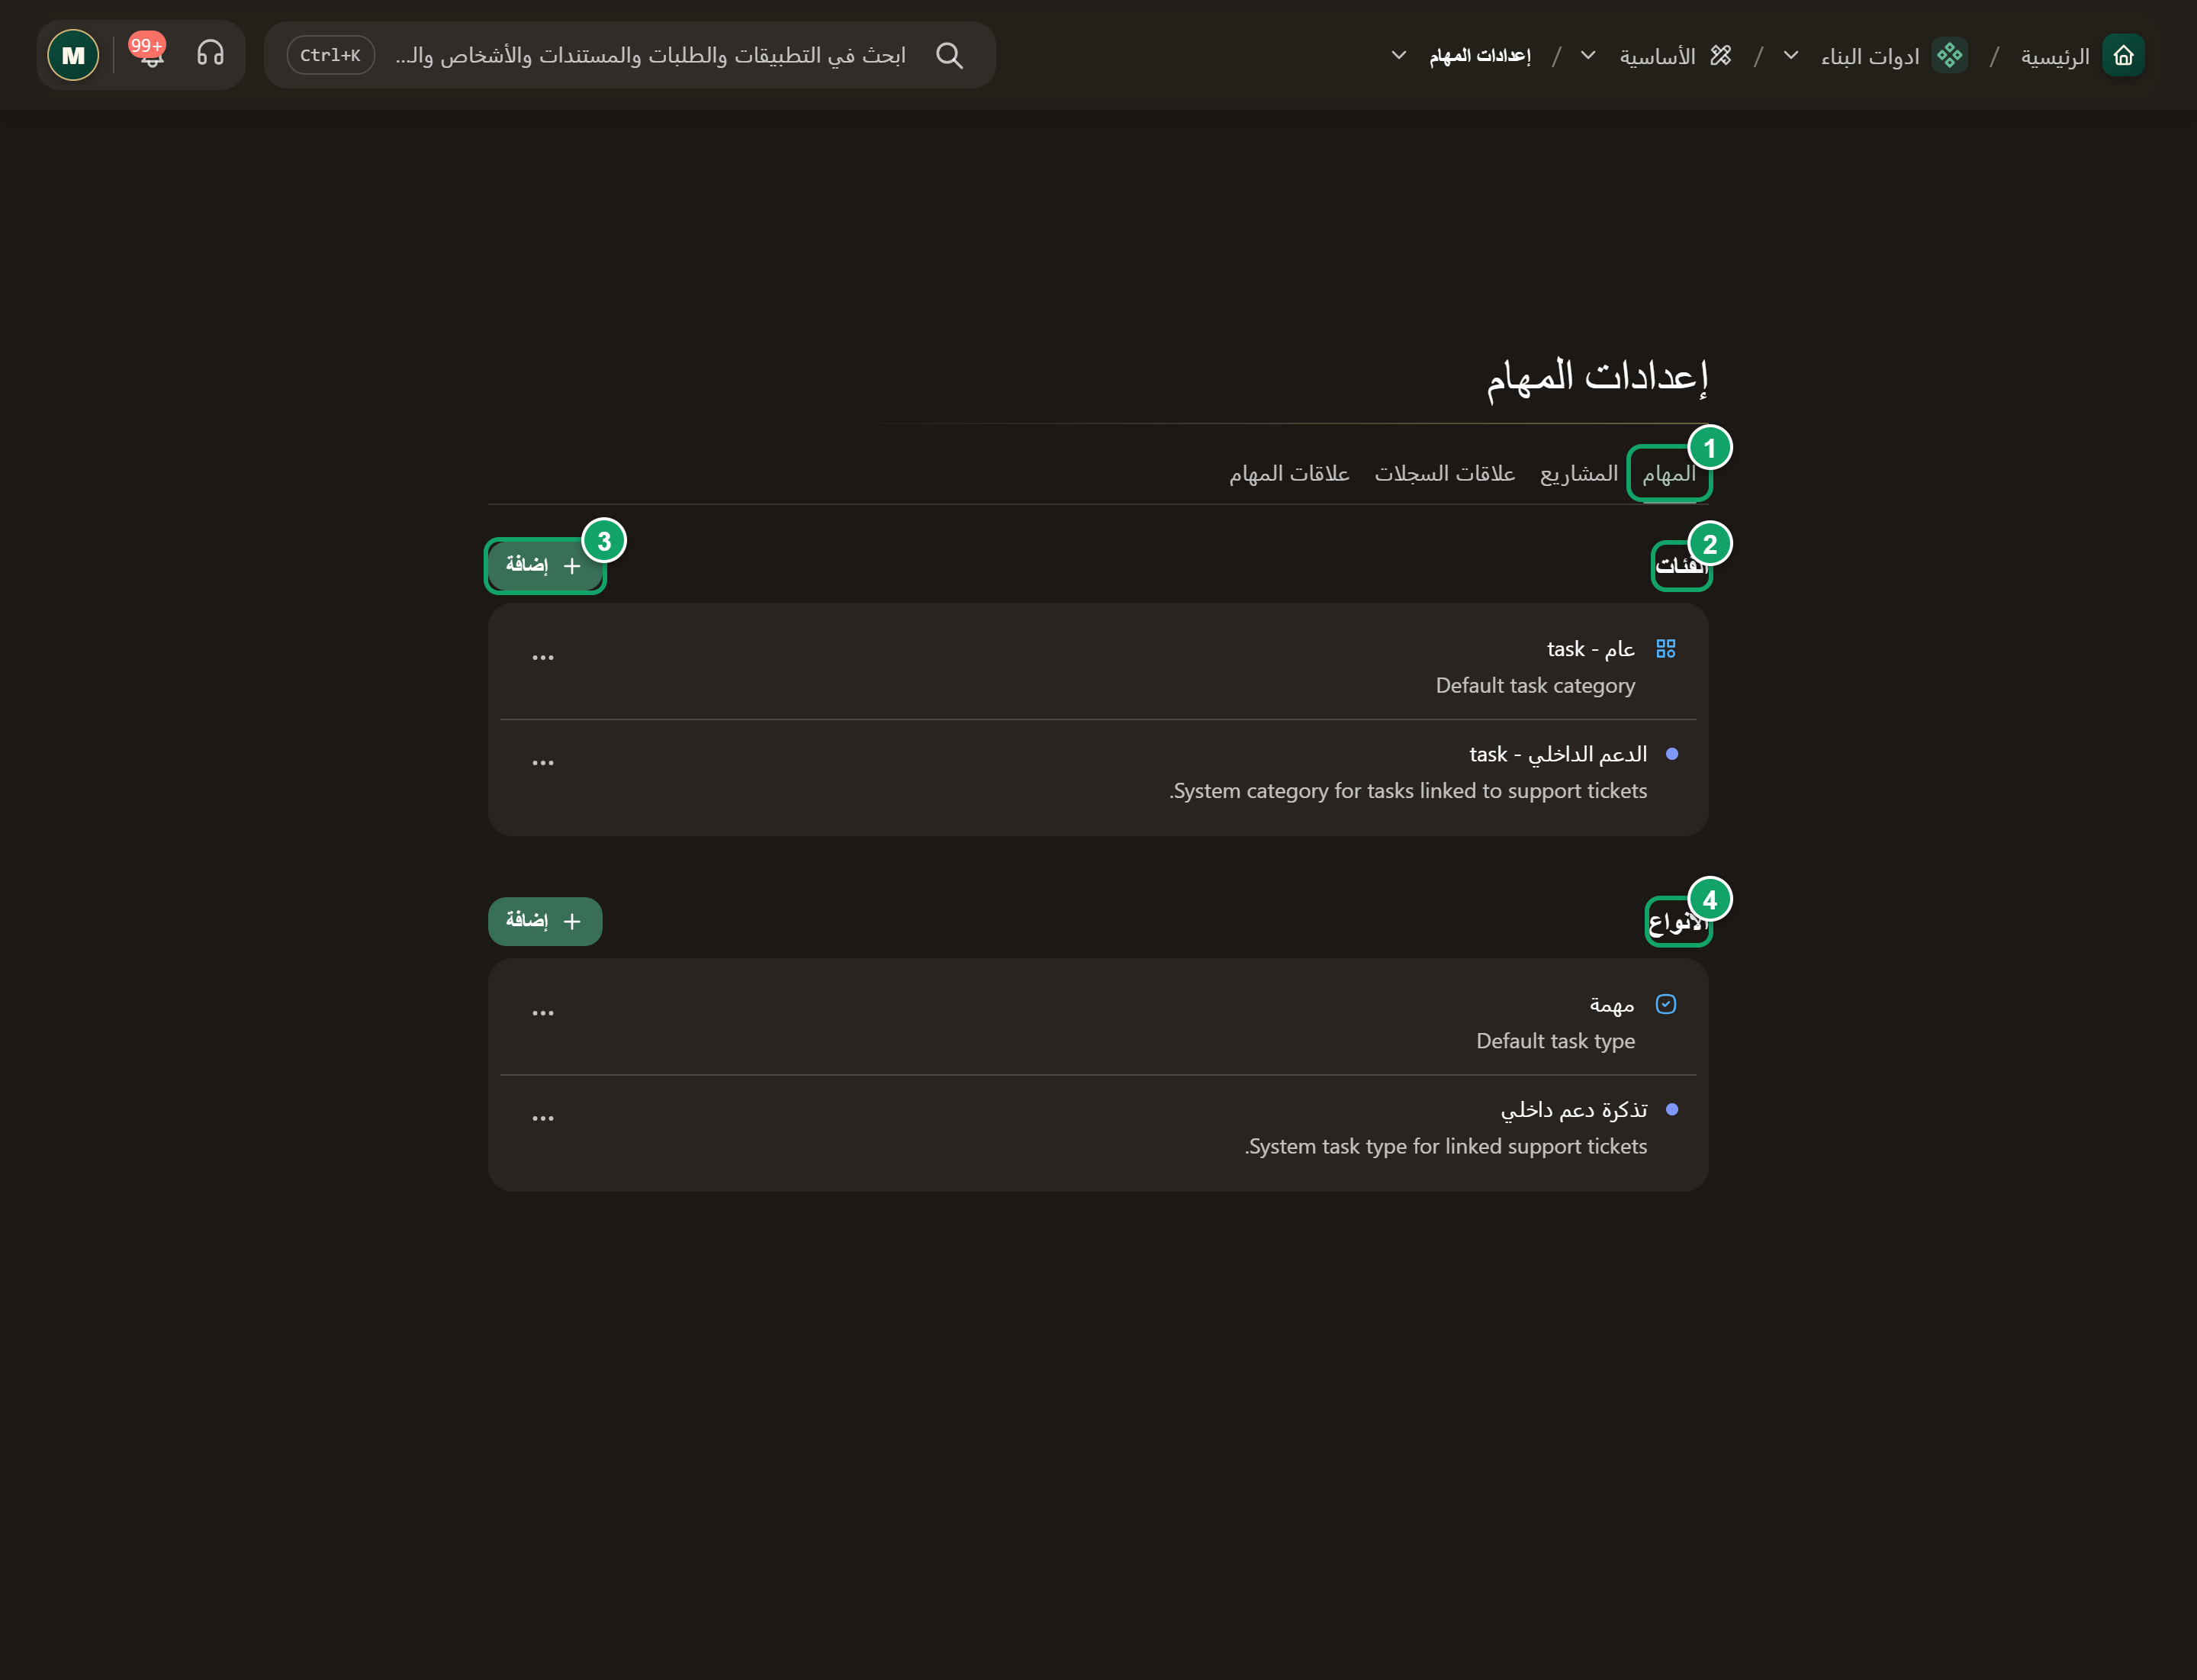
\includegraphics[width=0.95\linewidth,height=0.72\textheight,keepaspectratio]{figures/screens/ch04-settings-ar.png}
\caption{إعدادات أنواع المهام}
\label{fig:tasks-settings-settings}
\shotnote{تقسم «إعدادات المهام» التهيئة إلى أربعة تبويبات: «المهام» و«المشاريع» و«علاقات السجلات» و«علاقات المهام». ويعرض تبويب «المهام» الفئات والأنواع التي يختار منها المستخدم عند إنشاء مهمة، ومنها الفئة والنوع الافتراضيان. ولأن أي تعديل هنا يمس كل مهمة تستخدم النوع، فراجع أثره قبل تغييره. ① تبويب «المهام». ② «الفئات». ③ «إضافة»: ينشئ فئة جديدة. ④ «الأنواع»: تحدد شكل كل مهمة.}
\end{figure}

\begin{figure}[H]
\centering
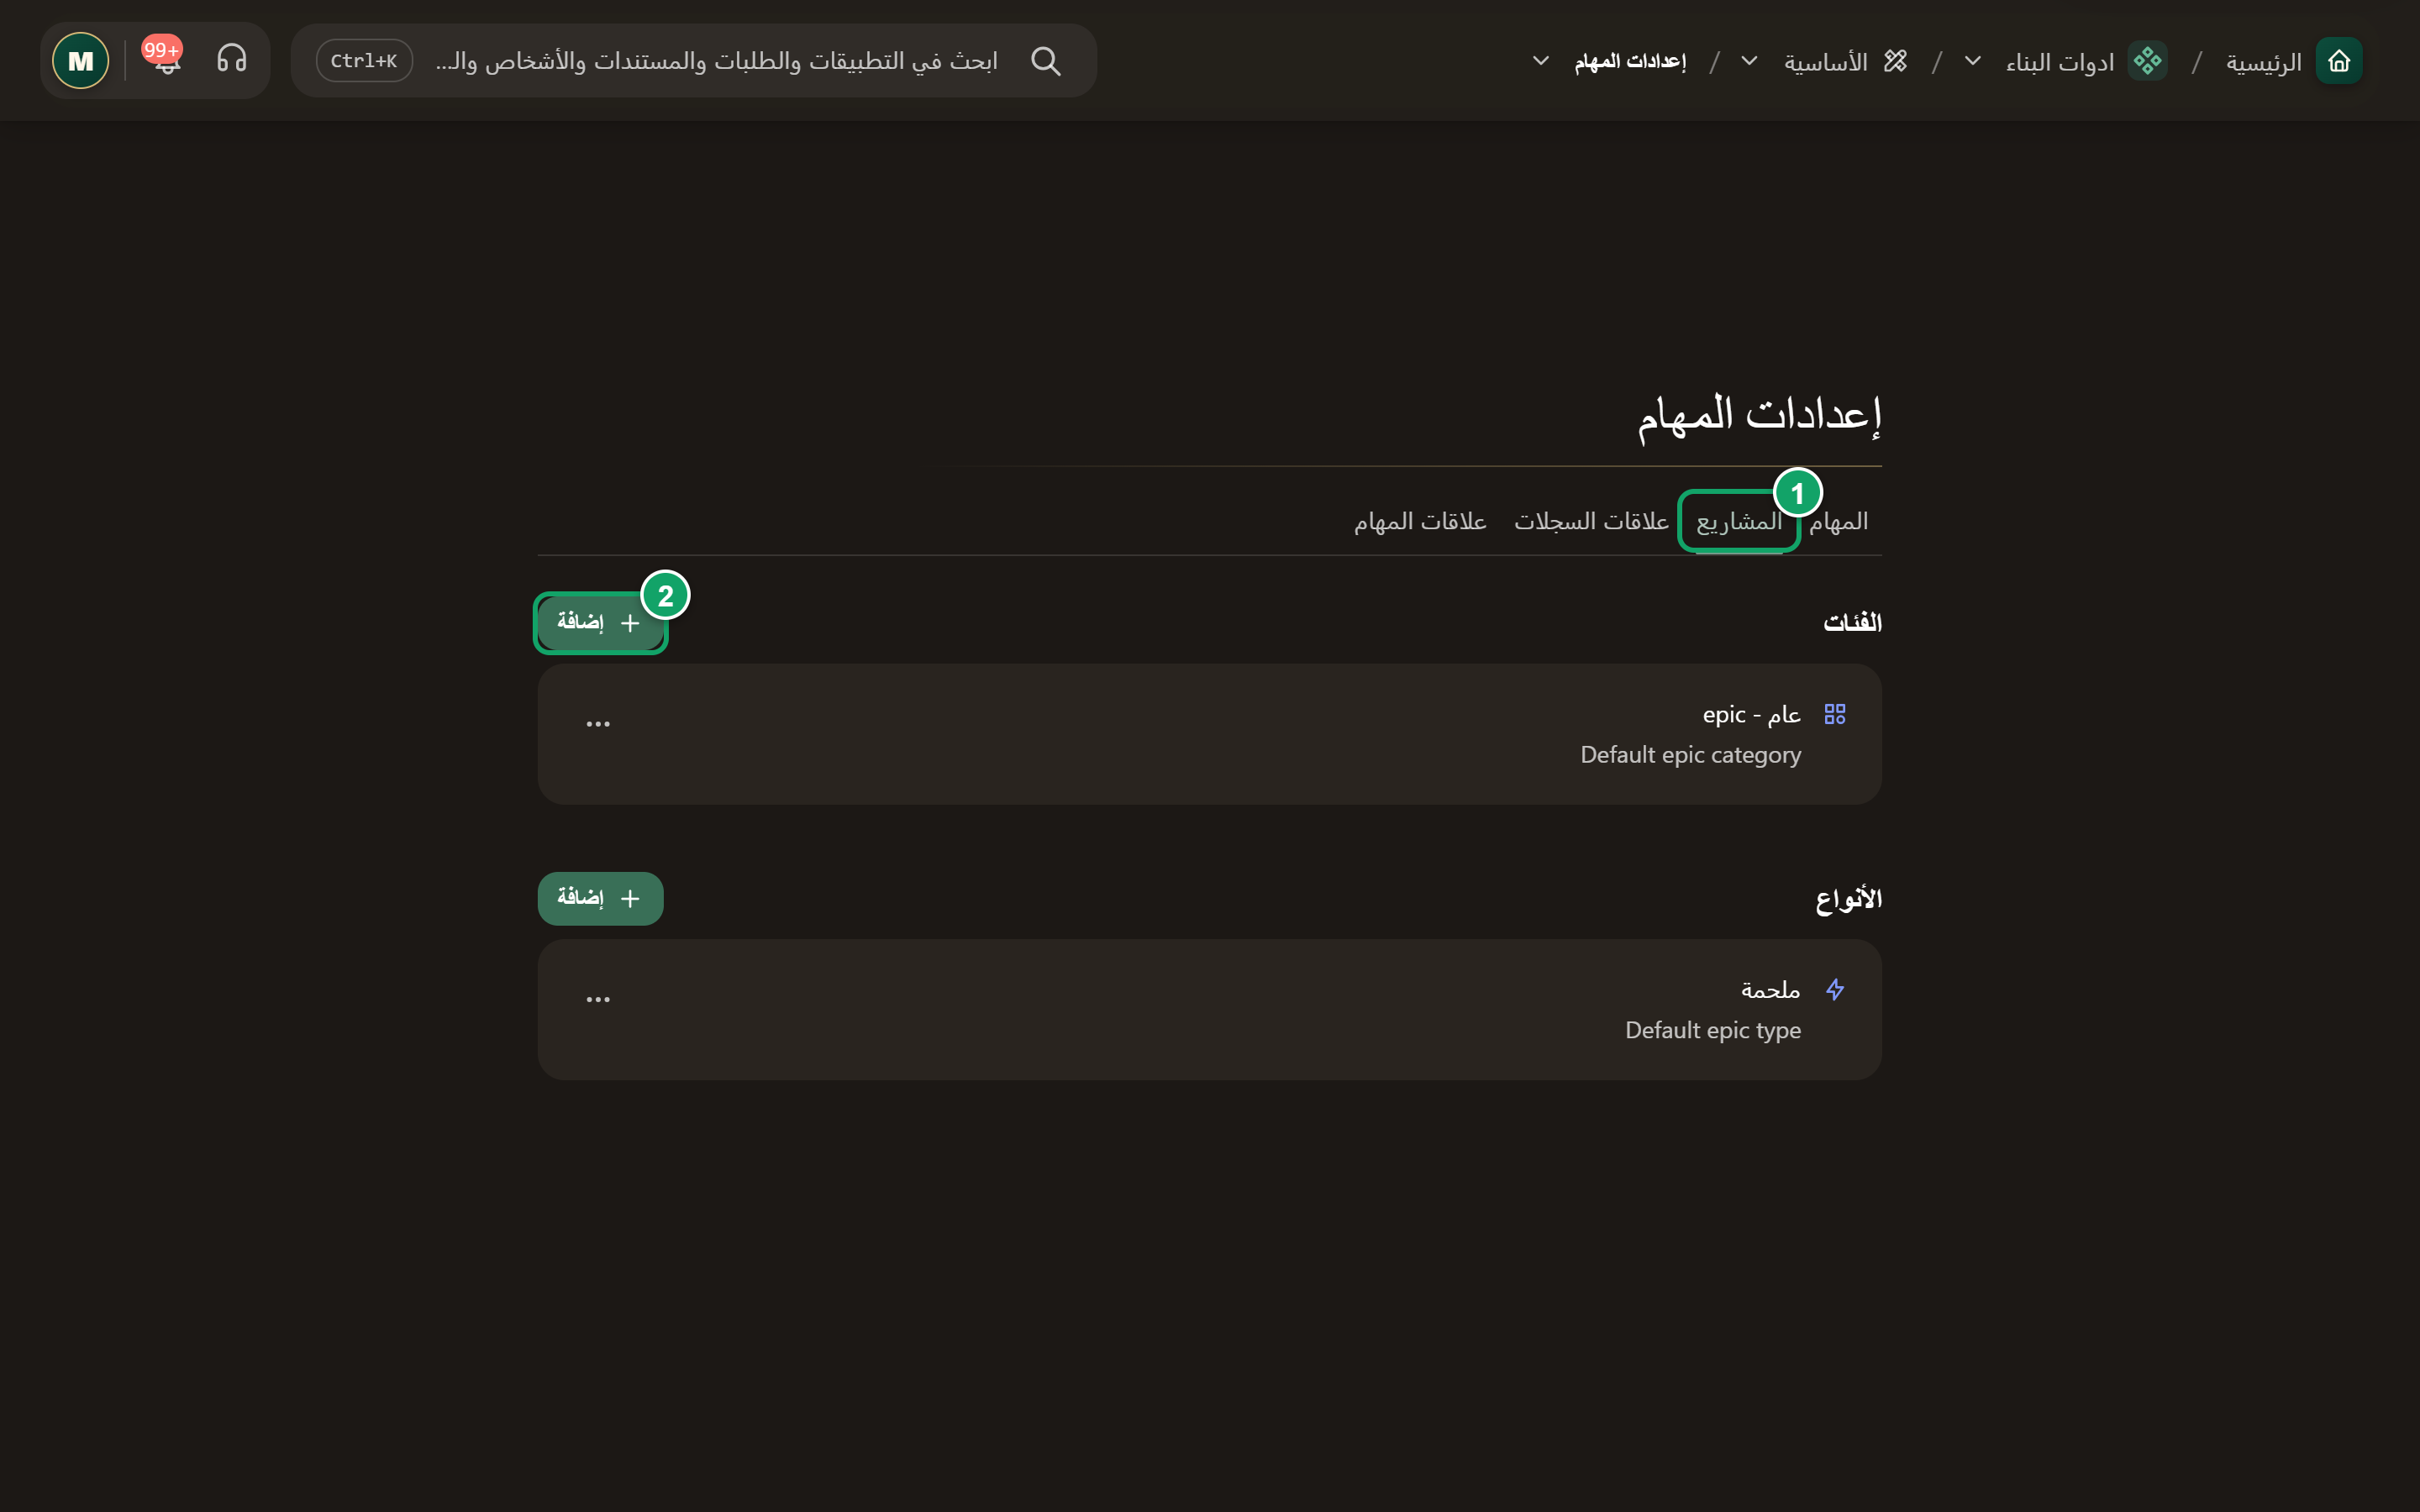
\includegraphics[width=0.95\linewidth,height=0.72\textheight,keepaspectratio]{figures/screens/ch04-settings-epics-ar.png}
\caption{إعدادات المهام الكبرى}
\label{fig:tasks-settings-settings-epics}
\shotnote{يضبط تبويب «المشاريع» هنا فئات المهام الكبرى وأنواعها بمعزل عن فئات المهام العادية، ويظهر في test2 النوع الافتراضي «ملحمة». ولا صلة لهذا التبويب بتطبيق المشاريع والتخطيط رغم تشابه الاسم. ① تبويب «المشاريع». ② «إضافة»: ينشئ إعداداً جديداً للمهام الكبرى.}
\end{figure}

\begin{figure}[H]
\centering
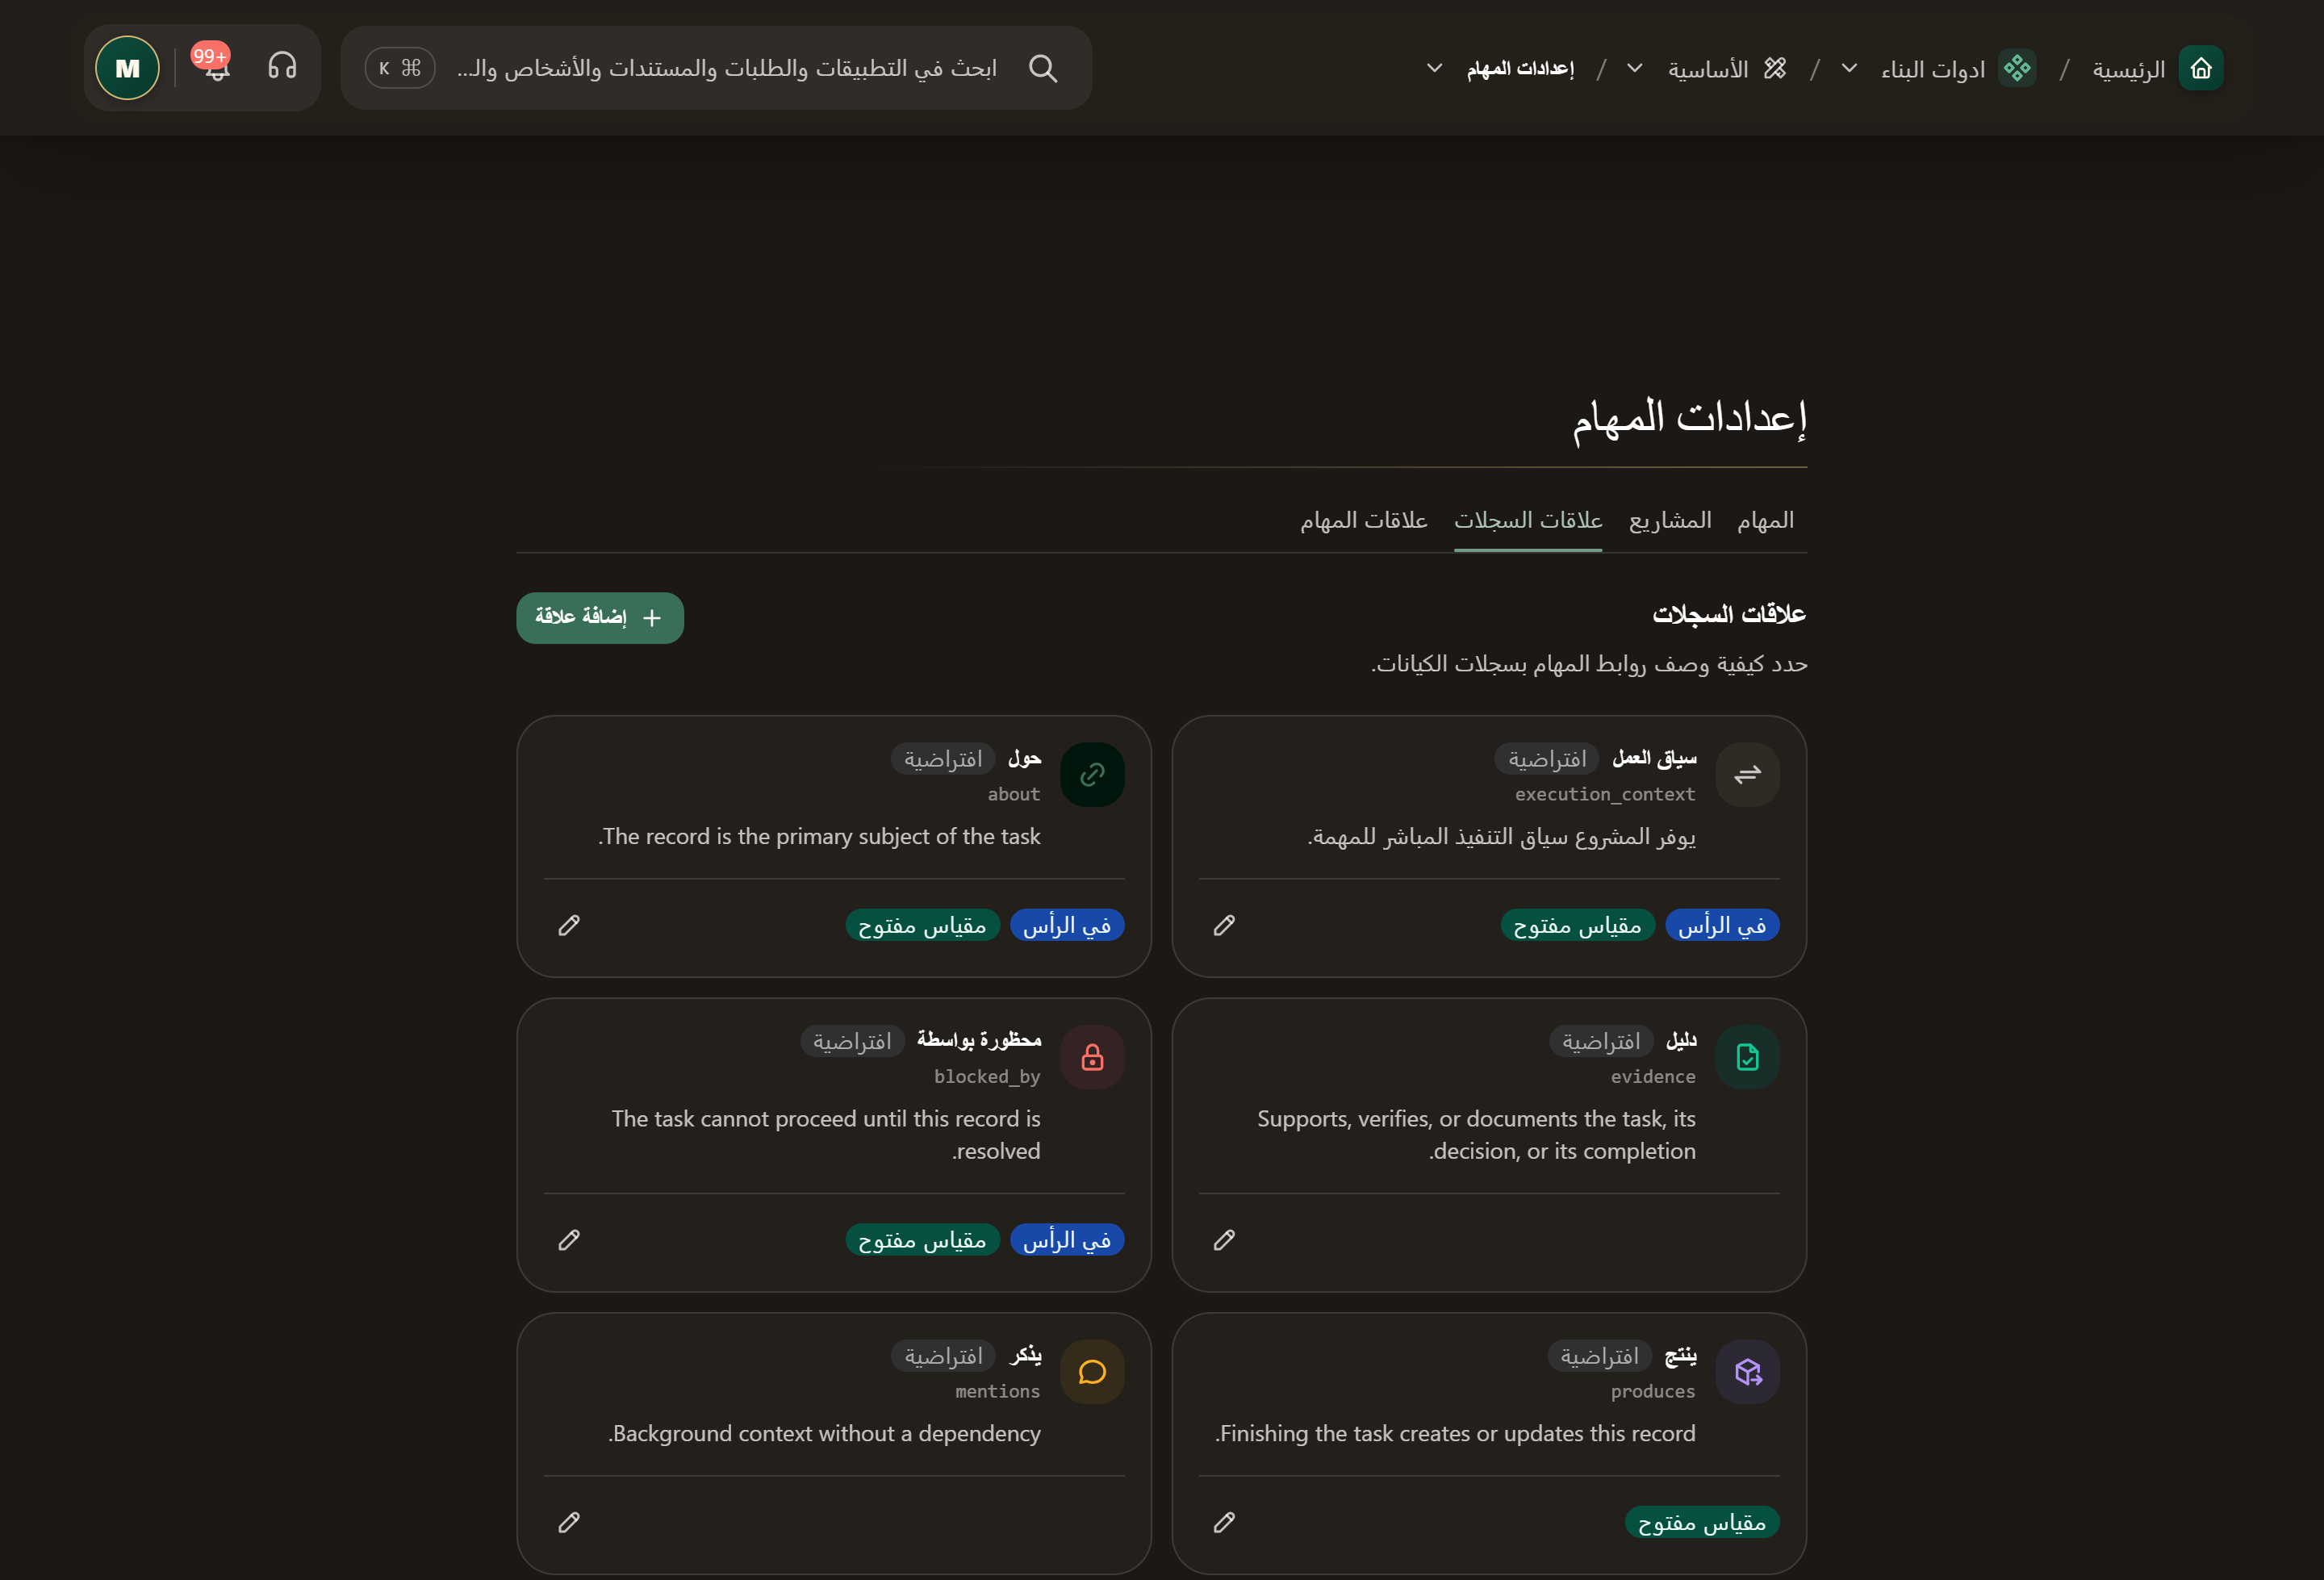
\includegraphics[width=0.95\linewidth,height=0.72\textheight,keepaspectratio]{figures/screens/ch04-settings-records-ar.png}
\caption{إعداد علاقات السجلات}
\label{fig:tasks-settings-settings-records}
\shotnote{يعرّف تبويب «علاقات السجلات» المعاني التي تختار منها عند ربط مهمة بسجل، مثل «دليل» و«ينتج» و«محظورة بواسطة»، ولكل معنى وصف يشرح أثره. وبذلك يفهم الفريق سبب الرابط لا مجرد وجوده. وتظهر هنا الأنواع الافتراضية، ويضيف المسؤول غيرها من «إضافة علاقة». ① تبويب «علاقات السجلات». ② «إضافة علاقة»: ينشئ نوعاً جديداً لربط المهام بالسجلات.}
\end{figure}

\begin{figure}[H]
\centering
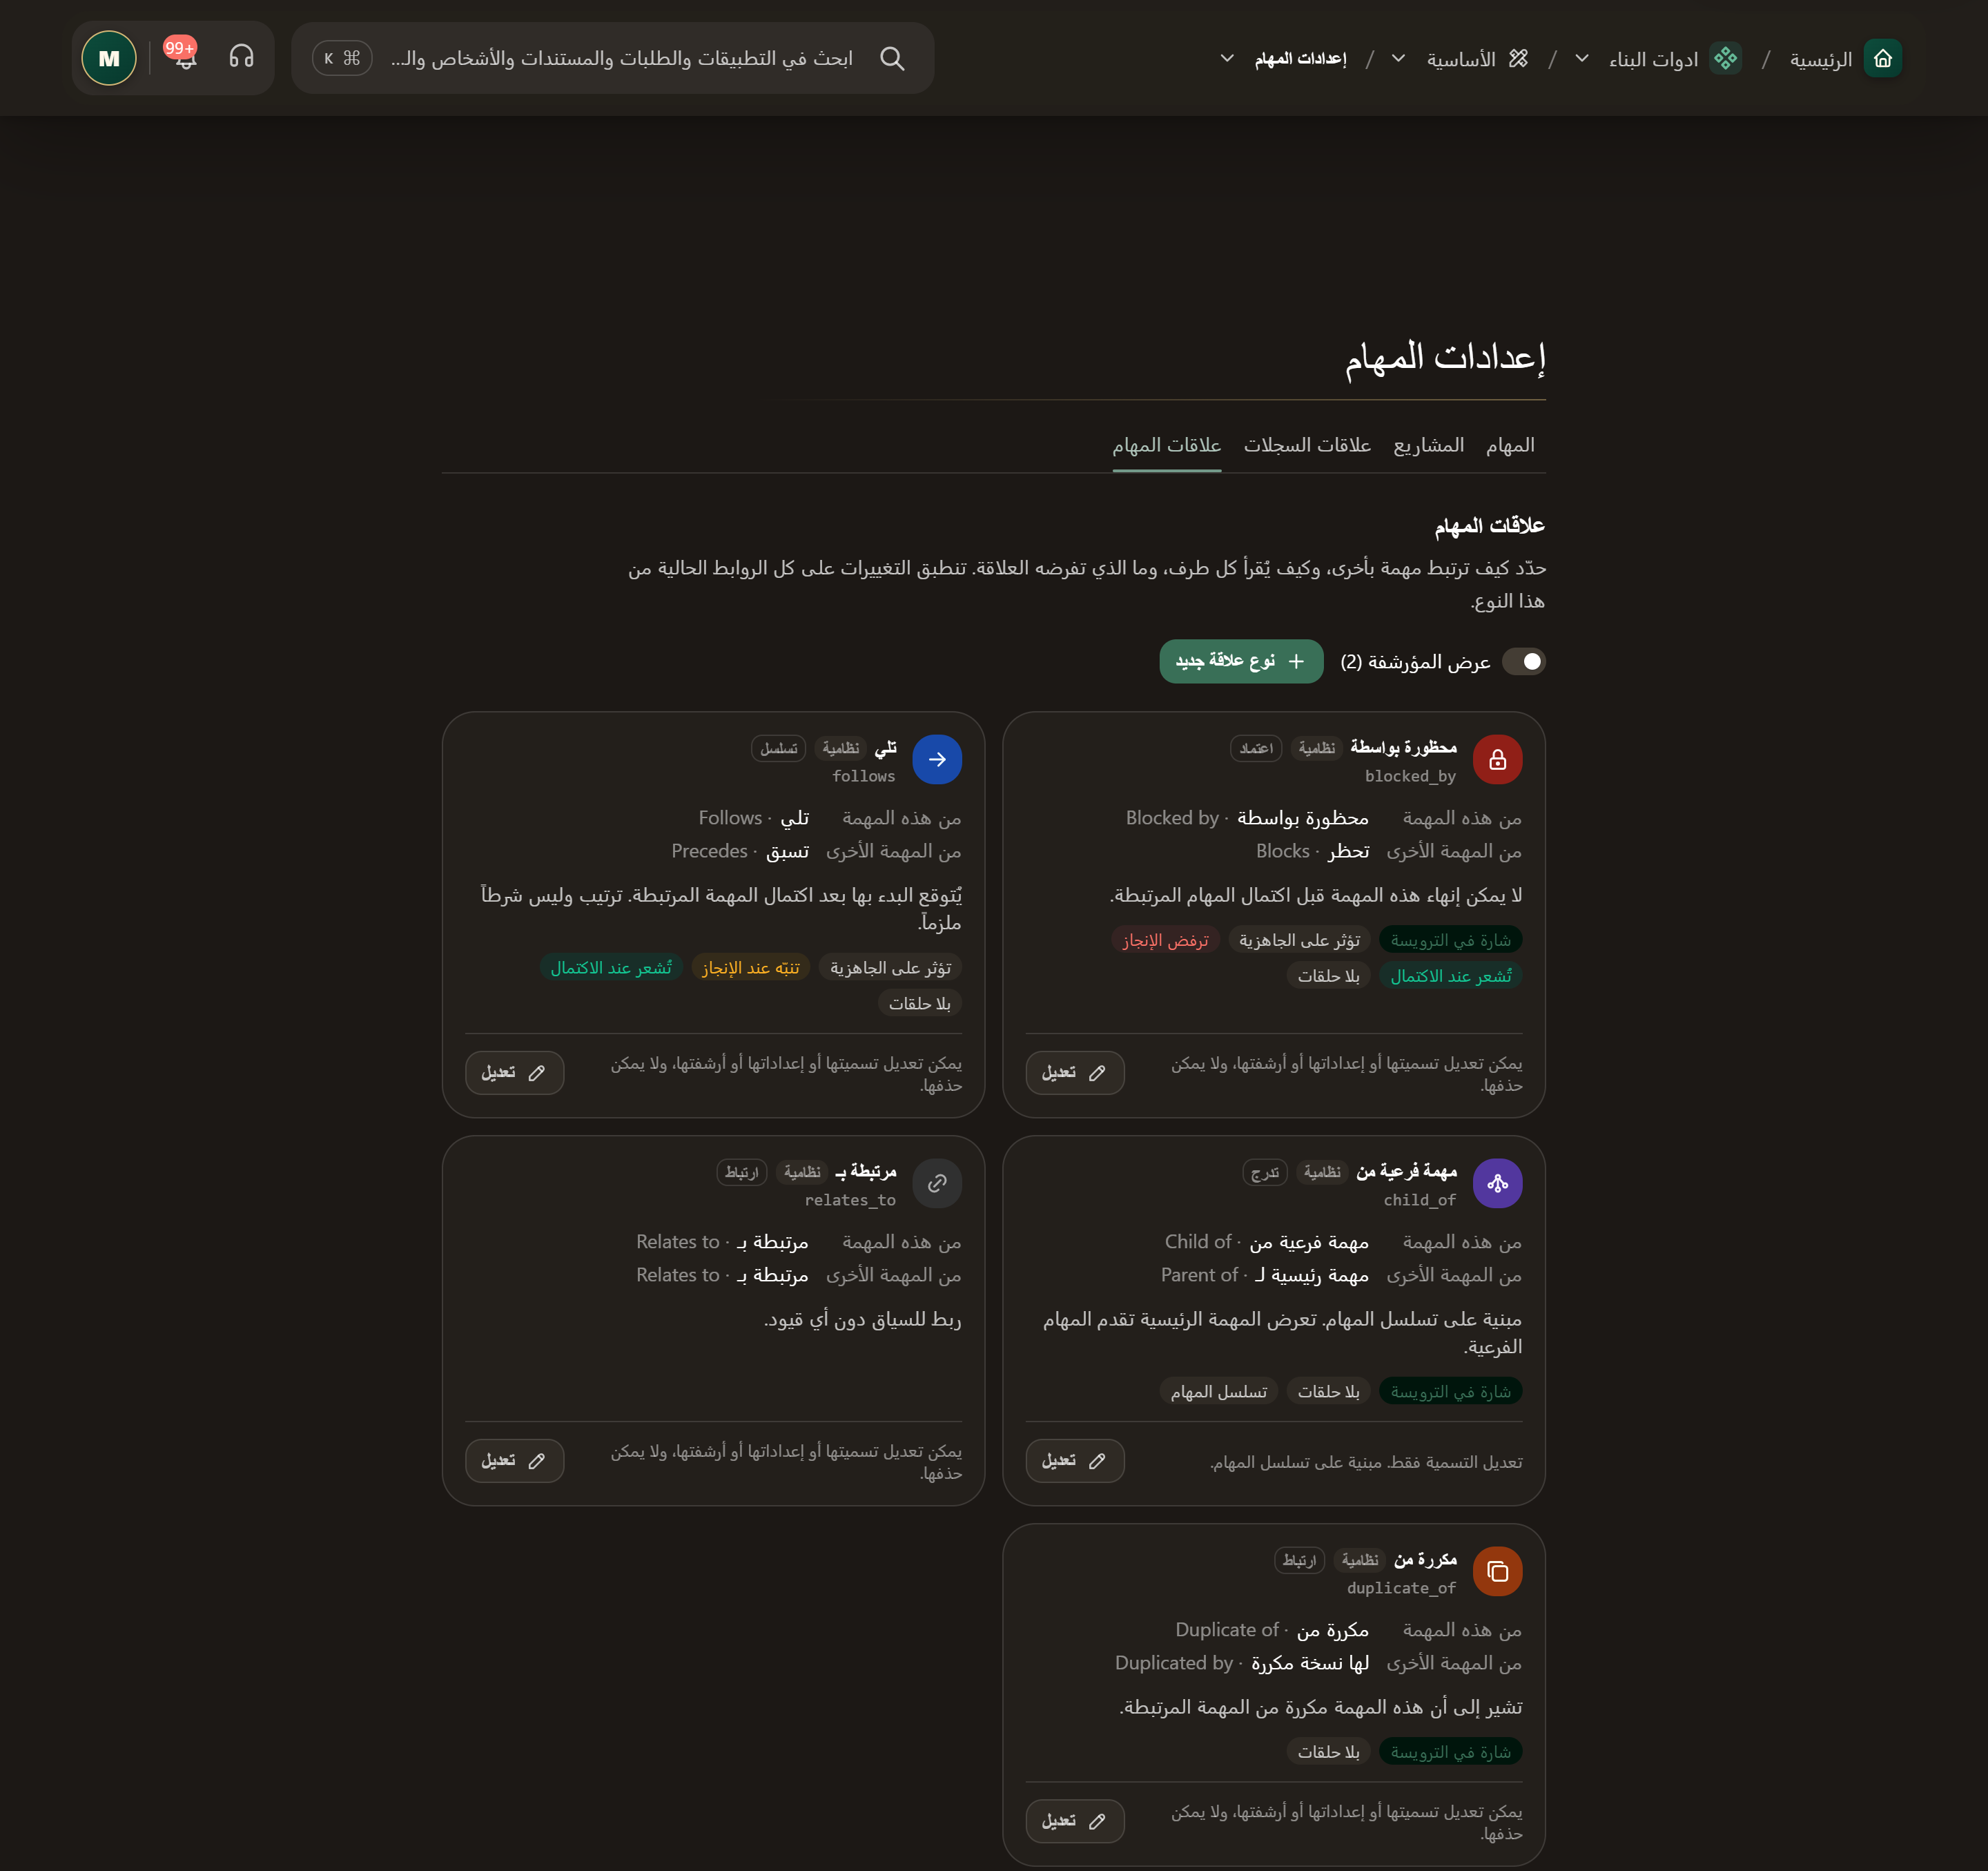
\includegraphics[width=0.95\linewidth,height=0.72\textheight,keepaspectratio]{figures/screens/ch04-settings-relations-ar.png}
\caption{إعداد علاقات المهام}
\label{fig:tasks-settings-settings-relations}
\shotnote{يحدد تبويب «علاقات المهام» كيف ترتبط مهمة بأخرى وكيف تُقرأ العلاقة من كل طرف، مثل «محظورة بواسطة» و«مهمة فرعية من». وتختلف آثارها: فعلاقة الحجب وحدها تحمل هنا شارة «ترفض الإنجاز»، بينما يكتفي غيرها بالترتيب أو الربط. ويمكن تعديل تسمية العلاقات النظامية أو أرشفتها، لكن لا يمكن حذفها. ① تبويب «علاقات المهام». ② «نوع علاقة جديد»: ينشئ نوعاً جديداً لربط المهام بعضها ببعض.}
\end{figure}

\begin{table}[H]
\centering
\caption{ما الذي تجده هنا؟}
\label{tab:tasks-settings-data}
\begin{tabularx}{\linewidth}{R{3.6cm} Y}
\rcHeaderRow
\thh{القسم} & \thh{المحتوى والإجراء}\\
المهام والمهام الكبرى & فئات وأنواع مستقلة لكل منهما، ولكل منها اسم ووصف ولون وأيقونة. ويحدد النوع الفئة وقالب الحالات الافتراضيين ومن يُسمح له باستخدامه.\\
قواعد النوع & العلاقات المطلوبة وحدودها، وإعدادات تحديث التقدم وتواتره بحسب الخيارات المتاحة.\\
علاقات السجلات والمهام & أنواع العلاقات وتسمياتها واتجاهها وقيودها. ميّز العلاقة العادية من العلاقة التي تمنع الإكمال.\\
\end{tabularx}
\end{table}

\begin{figure}[H]
\centering
\begin{tikzpicture}[node distance=0.5cm]
\node[stepBox] (a) {\RL{مراجعة النوع}};
\node[stepBox,below=of a] (b) {\RL{تحديد القواعد}};
\node[stepBox,below=of b] (c) {\RL{اختبار مهمة}};
\draw[flowsTo] (a) -- (b);
\draw[flowsTo] (b) -- (c);
\end{tikzpicture}
\rclegend
\caption{خطوات الاستخدام}
\label{fig:tasks-settings-flow}
\shotnote{يبدأ المخطط من النوع لأن القواعد مرتبطة به: راجع النوع، ثم حدد قواعده، ثم أنشئ مهمة اختبار بهذا النوع. فمهمة الاختبار تكشف أثر الإعداد في الحقول والانتقالات قبل أن يصل إلى عمل الفريق اليومي.}
\end{figure}

\subsection{خطوات العمل والتحقق}
\begin{enumerate}
\item افتح «إعدادات المهام» واختر تبويب «المهام»، أو «المشاريع» للمهام الكبرى، وراجع الفئات والأنواع الحالية قبل الإضافة.
\item افتح النوع، وراجع الاسم والفئة وقالب الحالات والسماح بالاستخدام، ثم راجع قواعد العلاقات والتقدم واحفظ التغييرات بعد اعتمادها.
\item أنشئ مهمة اختبار بهذا النوع في مجموعة مناسبة، وتحقق من ظهور الحقول والقواعد وانتقالات الحالة المتوقعة.
\end{enumerate}

\textbf{تحقق ومعالجة المشكلة:} إذا اختفى نوع من خيارات الإضافة، فراجع قيد المجموعة والسماح باستخدام النوع والصلاحيات. ولا تغيّر إعدادات مشتركة لتتجاوز خطأ في مهمة واحدة.

\clearpage
\section{قوالب الحالات}
\label{sec:tasks-feature-statuses}

يحدد قالب الحالات مراحل العمل والانتقالات بينها. ويُربط القالب بنوع المهمة حتى تسلك المهام مساراً يناسب طبيعة العمل.

\textbf{المسار ومن يستخدمه:} «أدوات البناء» ← «قوالب الحالات». يستخدمها المسؤول عن مسارات العمل.

\begin{rcnote}[مثال: شركة الأفق]
تحتاج مهام زيارات الأفق إلى بدء التنفيذ ثم مراجعة النتيجة، لذلك يراجع المسؤول قالبها مع سارة قبل أن يستخدمه الفريق.
\end{rcnote}

\begin{figure}[H]
\centering
\includegraphics[width=0.95\linewidth,height=0.72\textheight,keepaspectratio]{figures/screens/ch04-statuses-ar.png}
\caption{قائمة قوالب الحالات}
\label{fig:tasks-statuses-statuses}
\shotnote{تعرض «قوالب الحالات» كل القوالب المتاحة في المؤسسة مع إصدار كل قالب، ومنها قوالب تخدم الخطط وغيرها لا المهام وحدها. لذلك حدّد القالب الذي يستخدمه نوع مهمتك قبل أي تعديل؛ فهذه صفحة تهيئة مشتركة، وليست قائمة مهام الموظف. ① عنوان صفحة «قوالب الحالات». ② «إضافة»: ينشئ قالب حالات جديداً.}
\end{figure}

\begin{table}[H]
\centering
\caption{ما الذي تجده هنا؟}
\label{tab:tasks-statuses-data}
\begin{tabularx}{\linewidth}{R{3.6cm} Y}
\rcHeaderRow
\thh{القسم} & \thh{المحتوى والإجراء}\\
القالب والحالات & اسم القالب ومراحله ومعنى كل مرحلة. وتختلف أسماء الحالات بحسب إعداد المؤسسة.\\
الانتقالات & الإجراءات التي تنقل العمل بين المراحل، مع شروطها وصلاحياتها بحسب القالب.\\
الارتباط بالنوع & يختار نوع المهمة قالباً افتراضياً، لذلك راجع النوع بعد تعديل القالب.\\
تنظيم القوالب ونقلها & أنشئ «مجلد جديد» وانقل القوالب إليه، واستورد ملف JSON أو صدّره. وتتيح قائمة القالب التعديل أو الحذف بحسب الصلاحية.\\
\end{tabularx}
\end{table}

\begin{figure}[H]
\centering
\begin{tikzpicture}[node distance=0.5cm]
\node[stepBox] (a) {\RL{تعريف المراحل}};
\node[stepBox,below=of a] (b) {\RL{مراجعة الانتقالات}};
\node[stepBox,below=of b] (c) {\RL{الربط بالنوع والاختبار}};
\draw[flowsTo] (a) -- (b);
\draw[flowsTo] (b) -- (c);
\end{tikzpicture}
\rclegend
\caption{خطوات الاستخدام}
\label{fig:tasks-statuses-flow}
\shotnote{يرتب المخطط بناء المسار: عرّف المراحل أولاً، ثم راجع الانتقالات التي تنقل العمل بينها، وبعدها اربط القالب بالنوع وجرّبه. فلا يظهر أثر القالب في أي مهمة إلا من خلال نوع يستخدمه.}
\end{figure}

\subsection{خطوات العمل والتحقق}
\begin{enumerate}
\item افتح «قوالب الحالات» واختر القالب الذي يستخدمه نوع المهمة، وراجع مراحله وانتقالاته قبل التعديل.
\item راجع كل انتقال: من أي مرحلة يبدأ، وإلى أين يصل، ومن ينفّذه. واحفظ فقط التعديلات المعتمدة في مؤسستك.
\item ارجع إلى نوع المهمة وتحقق من القالب المختار، ثم جرّب المسار على مهمة اختبار.
\end{enumerate}

\textbf{تحقق ومعالجة المشكلة:} إذا غاب إجراء متوقع، فراجع المرحلة الحالية وشروط الانتقال والصلاحية. ولا تجعل تغيير اسم الحالة بديلاً عن تنفيذ الانتقال الصحيح.


\chapter{المشاريع والتخطيط}
\label{ch:projects}

\section{ماذا ستنجز؟}

ينظم تطبيق المشاريع العمل الذي يحتاج إلى خطة وموارد ونتائج يمكن مراجعتها. يحدد المسؤول الإعدادات والصلاحيات، ويضع مدير العمل الخطة ويتابع التنفيذ، ويحدّث الموظف السجلات المسندة إليه. ابدأ بالخطة عندما تحتاج إلى تحديد توجه أو نتيجة، وبالمشروع عندما يكون لديك عمل محدد النطاق تريد تسليمه.

\begin{rcnote}[مثال: شركة الأفق]
تستخدم سارة الخطيب خطة لتحسين جاهزية زيارات شركة الأفق، وتتابع مشروع تجهيز زيارة فرع حلب. يعدّ عمر حداد ملف الزيارة، ثم تراجع سارة المخرجات قبل اعتبار التحضير مكتملاً.
\end{rcnote}
\begin{figure}[H]
\centering
\begin{tikzpicture}[node distance=0.5cm]
\node[stepBox] (n0) {\RL{تحديد النتيجة والمسؤولية}};
\node[stepBox,below=of n0] (n1) {\RL{تهيئة العمل واعتماده}};
\node[stepBox,below=of n1] (n2) {\RL{التنفيذ والمراجعة}};
\draw[flowsTo] (n0) -- (n1);
\draw[flowsTo] (n1) -- (n2);
\end{tikzpicture}
\rclegend
\caption{من النتيجة المطلوبة إلى مراجعة التنفيذ}
\label{fig:projects-overview}
\shotnote{يضع المخطط تحديد النتيجة والمسؤولية قبل التنفيذ، ثم يربط المتابعة بما تحقق فعلياً. لا يعني هذا التسلسل أن إنشاء خطة ينشئ مشروعاً أو يوافق عليه تلقائياً؛ لكل سجل إجراءاته ومسؤوليته.}
\end{figure}

المحفظة تجمع برامج ومشاريع لخدمة أولويات مشتركة، والبرنامج ينسّق مشاريع مترابطة. هذه الروابط اختيارية في تعريف المشروع؛ لا تنشئ محفظة أو برنامجاً لمجرد الوصول إلى صفحة المشاريع. وتختلف الخطط والمشاريع هنا عن تبويب المهام الكبرى داخل تطبيق المهام.

\section{دليل صفحات المشاريع والتخطيط}
\label{sec:projects-pages}
\begin{figure}[H]
\centering
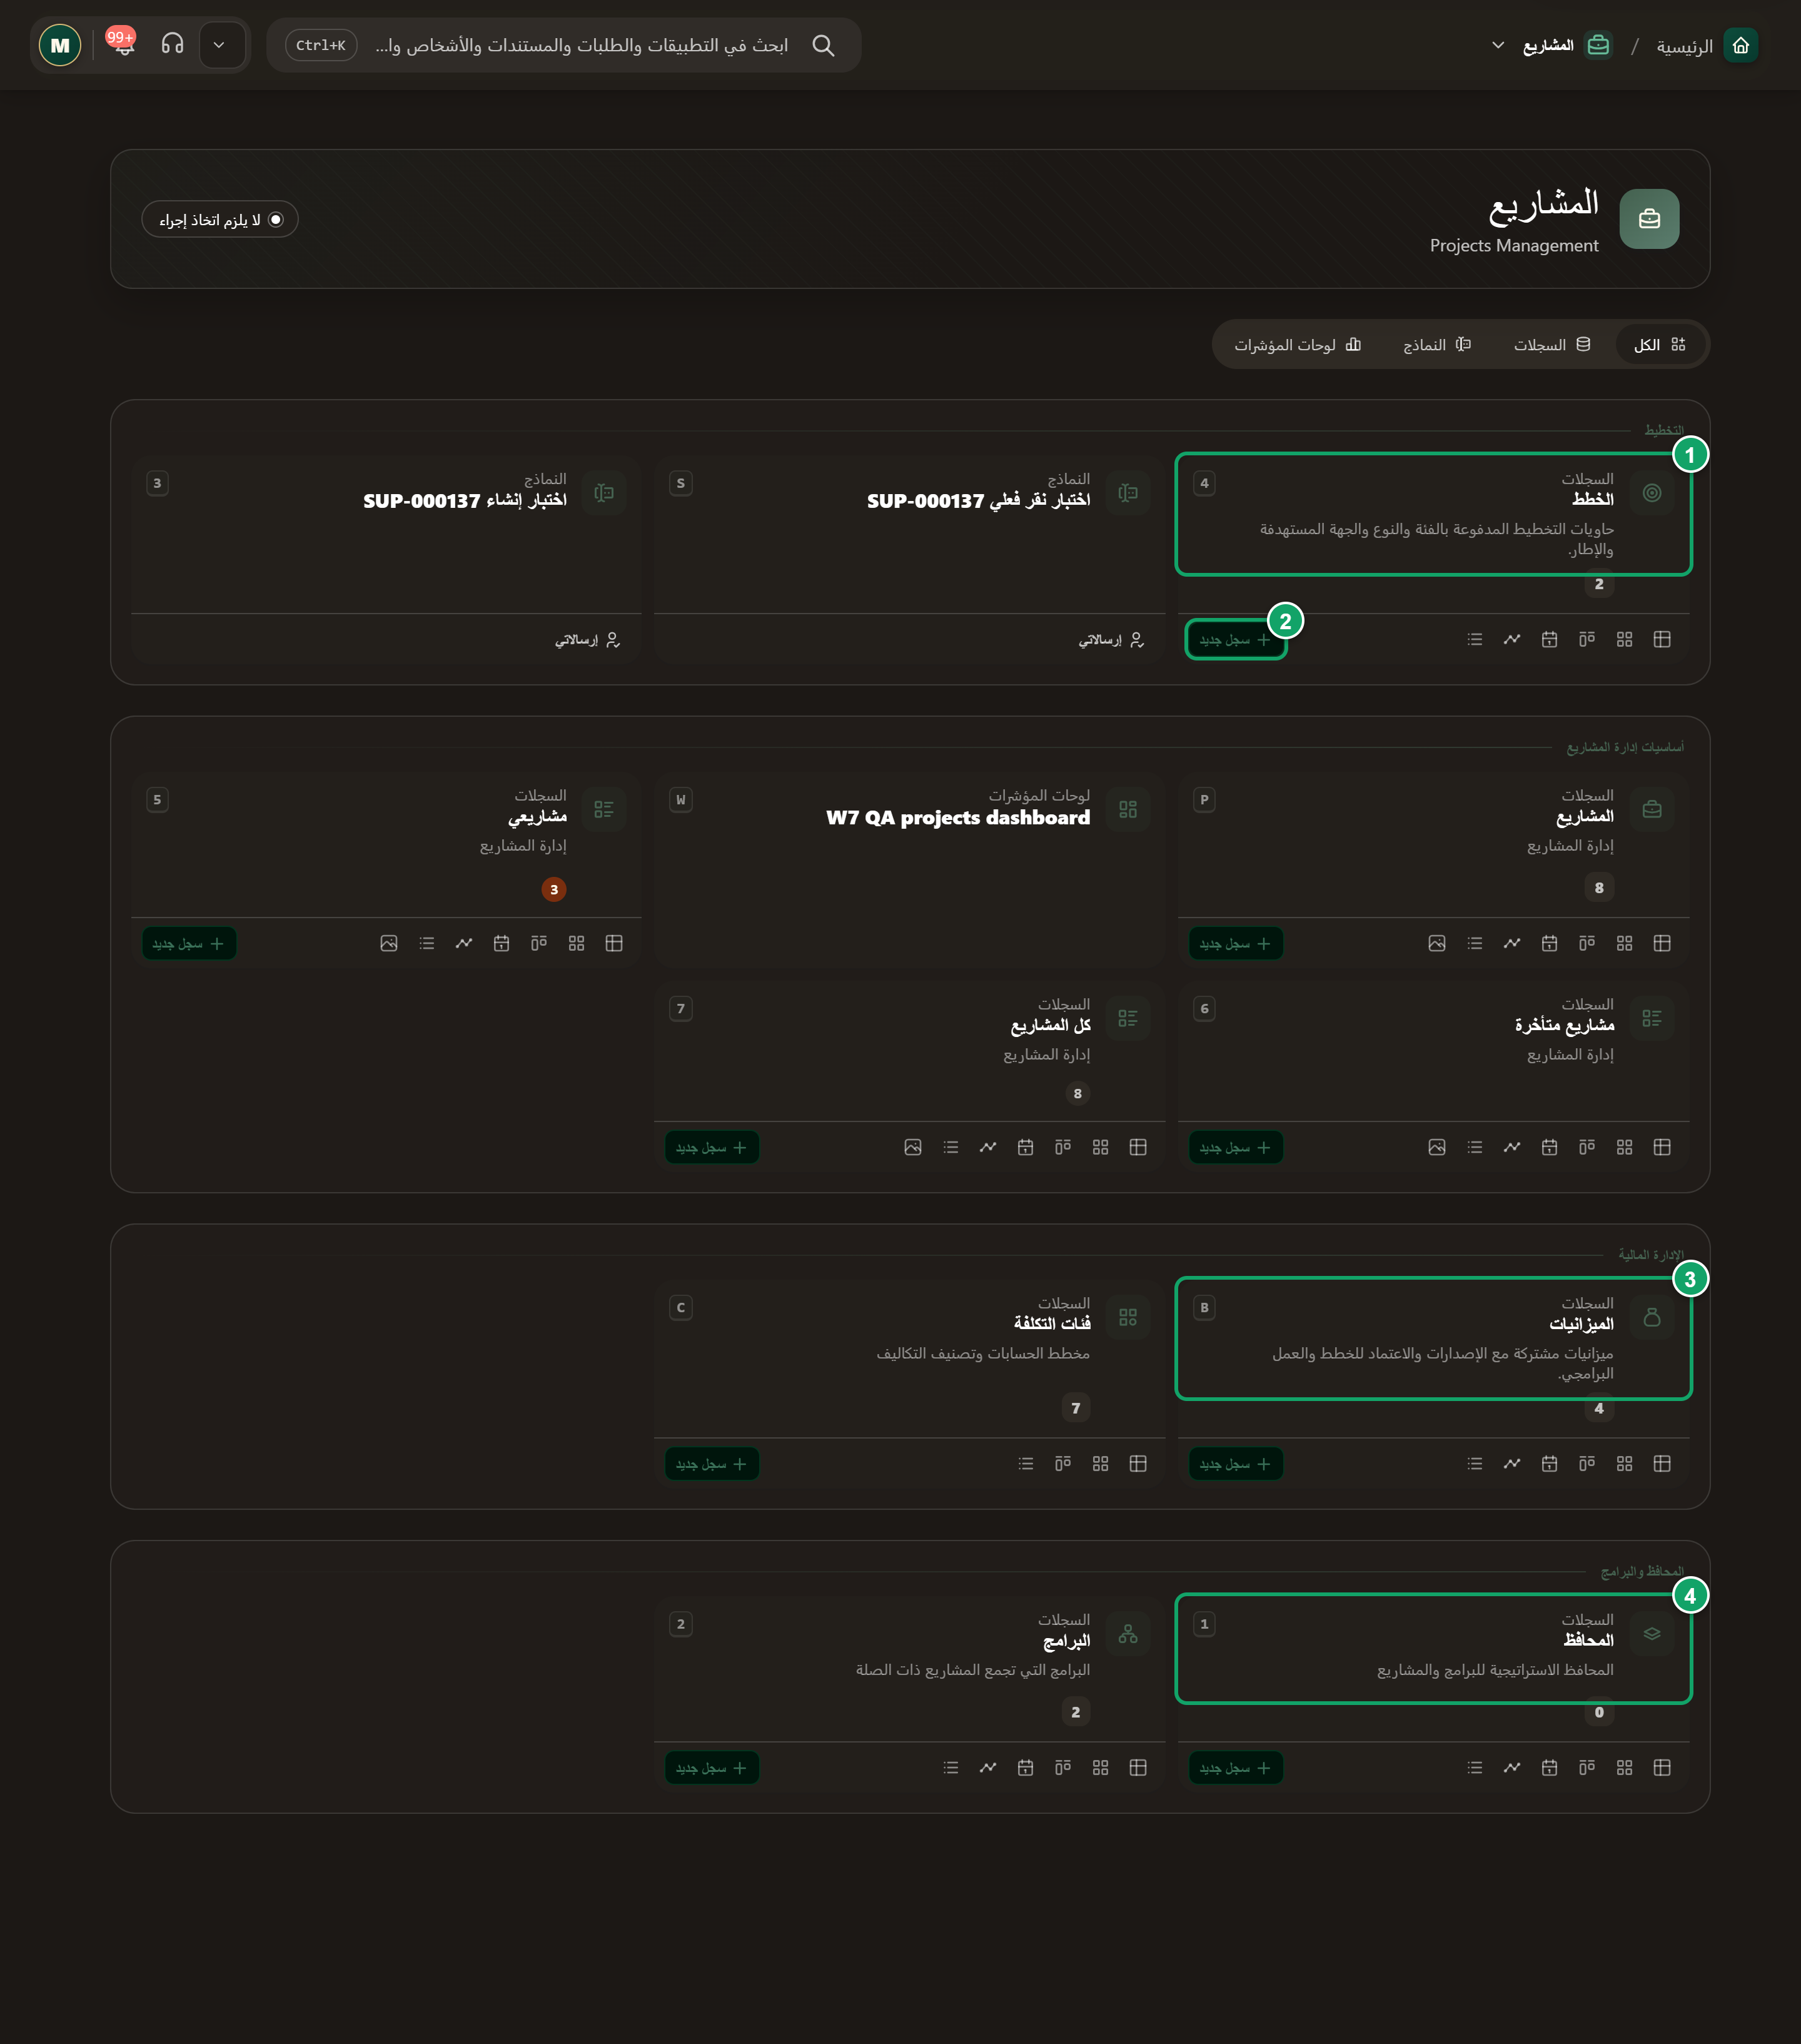
\includegraphics[width=0.95\linewidth,height=0.72\textheight,keepaspectratio]{figures/screens/ch05-directory-ar.png}
\caption{مدخل تطبيق المشاريع في بيئة الاختبار}
\label{fig:projects-screen-directory}
\shotnote{تعرض بطاقات التطبيق الصفحات الست الأساسية والعروض المخصصة المتاحة للحساب. العروض مثل المشاريع المسندة إليّ تعرض سجلات المشاريع نفسها، وليست نوعاً جديداً من السجلات؛ وقد تختلف البطاقات والأعداد باختلاف الصلاحيات والنطاق المختار. ① بطاقة «الخطط» تفتح قائمة الخطط. ② «سجل جديد»: ينشئ سجلاً مباشرة من البطاقة دون فتح القائمة. ③ بطاقة «الميزانيات» في قسم الإدارة المالية. ④ بطاقة «المحافظ» في قسم المحافظ والبرامج.}
\end{figure}

ابدأ بالصفحات الرئيسية، ثم افتح شرح السجل الذي تحتاج إليه من المجموعات التالية. بقية الصفحات تشرح سجلات أو أدوات داخل تبويبات، وليست كلها مداخل مستقلة في قائمة التطبيق. استخدم البحث والفلاتر والعروض المتاحة في القوائم للوصول إلى السجل؛ ولا تغيّر الفلاتر السجل نفسه.
\begin{table}[H]
\centering
\caption{الصفحات الرئيسية}
\label{tab:projects-pages-foundations}
\begin{tabularx}{\linewidth}{R{4.2cm} Y}
\rcHeaderRow
\thh{الصفحة} & \thh{ماذا تقدم هذه الصفحة؟}\\
الخطط & تجمع الخطة النتيجة المطلوبة والجهة المسؤولة والفترة التي ستعمل خلالها.\\
المشاريع & يجمع المشروع عملاً محدد النطاق له مدير ونتيجة مطلوبة.\\
المحافظ & تجمع المحفظة برامج ومشاريع تخدم توجهاً مشتركاً، وتساعد الإدارة على مراجعة الأولويات والتمويل.\\
البرامج & ينسّق البرنامج مشاريع مترابطة لتحقيق فائدة مشتركة.\\
الميزانيات & تجمع الميزانية بنود التكلفة ومصادر التمويل والمصروفات في سجل واحد.\\
فئات التكلفة & توحّد فئات التكلفة طريقة تصنيف بنود الميزانية، مثل السفر والتجهيزات.\\
\end{tabularx}
\end{table}
\begin{table}[H]
\centering
\caption{الأهداف والنتائج}
\label{tab:projects-pages-direction}
\begin{tabularx}{\linewidth}{R{4.2cm} Y}
\rcHeaderRow
\thh{الصفحة} & \thh{ماذا تقدم هذه الصفحة؟}\\
المحاور التخطيطية & يجمع المحور الاستراتيجي مجموعة من الأولويات تحت توجه واضح.\\
أهداف التخطيط & يصف الهدف التغيير الذي تريد الخطة تحقيقه.\\
المبادرات التخطيطية & تسجّل المبادرة عملاً مقترحاً يدعم التوجه الاستراتيجي.\\
دورات OKR & تجمع دورة الأهداف والنتائج الرئيسية أهداف فترة محددة والنتائج التي تقيس تحققها.\\
النتائج الرئيسية & تحوّل النتيجة الرئيسية الهدف إلى نتيجة قابلة للمتابعة.\\
متابعات النتائج الرئيسية & يسجّل تحديث النتيجة الرئيسية وضعها في تاريخ محدد.\\
عناصر هوشين & يربط أسلوب هوشين التوجهات طويلة المدى بالأهداف السنوية والعمل المطلوب.\\
روابط مصفوفة X لهوشين & توضح روابط مصفوفة هوشين كيف يدعم عنصرٌ عنصراً آخر.\\
تبادلات كاتشبّول لهوشين & تسجّل جولات التشاور المقترحات والردود حول عنصر من عناصر هوشين.\\
الإجراءات المضادة لهوشين & يسجّل الإجراء التصحيحي استجابةً لتعثر عنصر من عناصر هوشين.\\
افتراضات التخطيط & تسجّل الافتراضات أموراً تعتمد عليها الخطة ولم تُحسم بعد.\\
\end{tabularx}
\end{table}
\begin{table}[H]
\centering
\caption{التنفيذ والموارد}
\label{tab:projects-pages-delivery}
\begin{tabularx}{\linewidth}{R{4.2cm} Y}
\rcHeaderRow
\thh{الصفحة} & \thh{ماذا تقدم هذه الصفحة؟}\\
معالم التخطيط & يمثّل المعلم موعداً لنتيجة مهمة يمكن التحقق منها.\\
مراحل المشروع & تقسّم المرحلة المشروع إلى فترات عمل مرتبة يمكن مراجعة نهايتها.\\
هيكل العمل / حزم العمل & تقسّم حزمة العمل نطاق المشروع إلى جزء يمكن إسناده وتقدير جهده وتكلفته.\\
المخرجات / المنتجات & المخرج نتيجة أو منتج يمكن التحقق منه عند التسليم.\\
المتطلبات & يصف المتطلب ما يجب أن يحققه المشروع.\\
التبعيات & تربط علاقة الاعتماد عملاً سابقاً بعمل لاحق وتحدد نوع العلاقة الزمنية بينهما.\\
اعتماديات التخطيط & تسجّل علاقة الاعتماد ما ينتظر عملاً أو قراراً آخر داخل الخطة.\\
خطوط الأساس & يحفظ خط الأساس مرجعاً للمقارنة بين الخطة المعتمدة وما يحدث لاحقاً.\\
عناصر خط الأساس & يمثّل عنصر خط الأساس قيمة محفوظة ضمن إصدار محدد.\\
موارد التخطيط & تسجّل موارد الخطة احتياجات الجهد والتكلفة والكمية والسعة.\\
أدوار الفريق & يسجّل دور الفريق مسؤولية عضو داخل المشروع ونسبة تخصيصه عند استخدامها.\\
مصفوفة المسؤوليات & توضح مصفوفة المسؤوليات من ينفّذ النشاط ومن يتحمل مسؤوليته ومن يُستشار ومن يُطلع.\\
تخصيص الموارد & يسجّل تخصيص المورد السعة المحجوزة للعمل وما استُخدم منها.\\
أصحاب المصلحة & يجمع سجل أصحاب المصلحة الأشخاص أو الجهات المعنية بالمشروع ودرجة اهتمامهم وتأثيرهم.\\
خطة الاتصال & تحدد خطة التواصل ما سيُعرض ولمن وبأي نوع من التواصل.\\
\end{tabularx}
\end{table}
\begin{table}[H]
\centering
\caption{المراجعة والجودة والمخاطر}
\label{tab:projects-pages-governance}
\begin{tabularx}{\linewidth}{R{4.2cm} Y}
\rcHeaderRow
\thh{الصفحة} & \thh{ماذا تقدم هذه الصفحة؟}\\
مراجعات التخطيط & توثّق المراجعة ما جرى تقييمه خلال فترة محددة وحالة تلك المراجعة.\\
اعتمادات التخطيط & يسجّل سجل الموافقة المرحلة والقرار المتعلقين بالخطة.\\
قرارات التخطيط & يحفظ سجل القرار ما تقرر وسبب متابعته ضمن الخطة.\\
سجل المخاطر & يسجّل الخطر حدثاً محتملاً قد يؤثر في الخطة.\\
سجل مخاطر إدارة المشاريع & يسجّل خطر المشروع احتمالاً قد يؤثر في التسليم، مع تقدير الأثر وخطة الاستجابة.\\
المشكلات & تسجّل المسألة مشكلة قائمة تحتاج إلى حل، بخلاف الخطر الذي قد يقع لاحقاً.\\
معايير الجودة & يحدد معيار الجودة كيف ستتحقق من صلاحية نتيجة العمل.\\
مراجعات البوابة & تسجّل مراجعة البوابة قرار الانتقال عند نقطة مهمة في المشروع.\\
فحوصات مراجعة البوابة & يسجّل فحص البوابة نتيجة معيار واحد من معايير المراجعة.\\
طلبات التغيير & يحفظ طلب التغيير التعديل المقترح وأثره على المشروع ومسار مراجعته.\\
قرارات الاجتماعات & يسجّل قرار الاجتماع ما اتُّفق عليه وما يحتاج إلى متابعة.\\
الدروس المستفادة & يحفظ الدرس المستفاد تجربة يمكن أن تفيد أعمالاً لاحقة.\\
تقارير الحالة & يجمع تقرير الحالة التقدم والمخاطر والملاحظات خلال فترة محددة.\\
\end{tabularx}
\end{table}
\begin{table}[H]
\centering
\caption{العمل الرشيق}
\label{tab:projects-pages-agile}
\begin{tabularx}{\linewidth}{R{4.2cm} Y}
\rcHeaderRow
\thh{الصفحة} & \thh{ماذا تقدم هذه الصفحة؟}\\
السباقات & يقسّم السباق العمل الرشيق إلى فترة محددة لها هدف ومراجعة.\\
إدخالات احتراق السبرنت & يسجّل قياس العمل المتبقي عدد النقاط في يوم محدد من السباق.\\
تعريف الإنجاز & تحدد معايير الإنجاز ما يجب استيفاؤه قبل اعتبار العمل منتهياً.\\
\end{tabularx}
\end{table}
\begin{table}[H]
\centering
\caption{المشتريات والتمويل}
\label{tab:projects-pages-finance}
\begin{tabularx}{\linewidth}{R{4.2cm} Y}
\rcHeaderRow
\thh{الصفحة} & \thh{ماذا تقدم هذه الصفحة؟}\\
المشتريات & يجمع سجل المشتريات الحاجة المطلوبة وبيانات التعاقد والمتابعة المالية.\\
بنود الميزانية & يفصّل بند الميزانية تكلفة محددة داخل الميزانية.\\
فترات بند الميزانية & توزّع فترات البند مبالغه على الزمن.\\
مصادر التمويل & يسجّل مصدر التمويل الجهة أو المصدر والمبلغ المتعهد به وشروطه.\\
دفعات التمويل & تسجّل دفعة التمويل ما خُطط لاستلامه وما استُلم من المصدر.\\
المصروفات & يسجّل المصروف تكلفة فعلية مرتبطة بمشروع وميزانية.\\
\end{tabularx}
\end{table}
\begin{table}[H]
\centering
\caption{القياس والتقييم والتعلم}
\label{tab:projects-pages-performance}
\begin{tabularx}{\linewidth}{R{4.2cm} Y}
\rcHeaderRow
\thh{الصفحة} & \thh{ماذا تقدم هذه الصفحة؟}\\
مؤشرات الأداء & يقيس المؤشر جانباً محدداً من الأداء بوحدة واتجاه قياس ووتيرة متابعة.\\
الأهداف المرحلية & توزّع المستهدفات الزمنية النتيجة المطلوبة على فترات.\\
فترات التقارير & تحدّد فترة التقرير الحدود الزمنية للقياسات والمراجعات.\\
مصادر بيانات التخطيط & يحدد مصدر البيانات من أين تأتي معلومات المتابعة والتقييم.\\
عناصر الأدلة & يحفظ سجل الدليل مرجعاً يدعم نتيجة أو استنتاجاً.\\
أسئلة التقييم & يحدد سؤال التقييم ما تريد معرفته ومعيار الحكم عليه.\\
نتائج التقييم & تسجّل نتيجة التقييم ما خلصت إليه المراجعة وما يترتب عليه.\\
استجابات الإدارة & تسجّل استجابة الإدارة ما ستفعله بشأن نتيجة تقييم أو ملاحظة تعلم.\\
بنود أجندة التعلم & يجمع جدول التعلم الأسئلة التي يحتاج الفريق إلى فهمها والأدلة المطلوبة لها.\\
رؤى التعلم & يسجّل استنتاج التعلم ما فهمه الفريق وكيف سيستفيد منه.\\
فرص التحسين & تبدأ فرصة التحسين بمشكلة واضحة يمكن معالجتها.\\
نظرية التغيير & تربط نظرية التغيير بين العمل والنتائج المتوقعة والافتراضات التي تقوم عليها.\\
أطر النتائج & يجمع إطار النتائج الأهداف والتغيرات والمخرجات والأنشطة في بنية مترابطة.\\
أهداف الإطار المنطقي & يصف الهدف الأعلى الأثر الواسع الذي يخدمه إطار النتائج.\\
نتائج الإطار المنطقي & تصف النتيجة التغيير المتوقع لدى الجهة المستفيدة من العمل.\\
مخرجات الإطار المنطقي & يمثّل المخرج نتيجة مباشرة يمكن تسليمها ضمن إطار النتائج.\\
أنشطة الإطار المنطقي & يسجّل النشاط العمل الذي ينتج مخرجاً محدداً.\\
المستفيدون & يسجّل المستفيدون الأشخاص أو الفئات التي يخدمها المشروع.\\
شرائح المستفيدين & تفصّل شرائح المستفيدين توزيع سجل المستفيدين وفق بُعد محدد.\\
\end{tabularx}
\end{table}
\begin{table}[H]
\centering
\caption{الاستمرارية والاستجابة}
\label{tab:projects-pages-resilience}
\begin{tabularx}{\linewidth}{R{4.2cm} Y}
\rcHeaderRow
\thh{الصفحة} & \thh{ماذا تقدم هذه الصفحة؟}\\
سيناريوهات التخطيط & يصف السيناريو ظرفاً محتملاً تحتاج الخطة إلى الاستعداد له.\\
سجلات تحليل أثر الأعمال & يوضح تحليل أثر الأعمال الخدمة المتأثرة ومدى أهميتها عند التعطل.\\
إجراءات التخطيط & تسجّل الإجراءات ما ينبغي عمله عند ظرف محدد ومدى الجاهزية لتنفيذه.\\
تمارين التخطيط & توثّق التمارين اختبار إجراء أو خطة استعادة قبل الحاجة الفعلية إليها.\\
ضوابط التخطيط & يسجّل الضابط إجراءً وقائياً أو رقابياً للحد من خطر أو متابعة التزام.\\
تقييمات الضوابط & يسجّل تقييم الضابط اختباراً أو مراجعة لفعاليته في تاريخ محدد.\\
ملاحظات التخطيط & توثّق الملاحظة خللاً ظهر في تدقيق أو مراجعة أو بعد حادث.\\
حوادث التخطيط & يسجّل الحادث مشكلة وقعت فعلاً وتحتاج إلى استجابة.\\
أحداث الخط الزمني للحوادث & يرتب سجل الأحداث ما وقع أثناء الحادث بحسب الوقت.\\
\end{tabularx}
\end{table}


\clearpage
\section{الخطط}
\label{sec:projects-feature-plans}

تجمع الخطة النتيجة المطلوبة والجهة المسؤولة والفترة التي ستعمل خلالها. يحدد نوع الخطة وإطارها الأقسام التي تحتاج إلى تعبئتها، لذلك ابدأ بتحديد ما تريد تحقيقه.

\begin{rcnote}[مثال: شركة الأفق]
تضع سارة خطة «تحسين جاهزية فرع حلب» وتختار الجهة المسؤولة عن الزيارات. يساعدها تحديد المالك والفترة على مراجعة العمل مع عمر قبل موعد الزيارة.
\end{rcnote}

\textbf{المسار ومن يستخدمه:} افتح تطبيق «المشاريع»، ثم بطاقة «الخطط». هذه صفحة رئيسية في التطبيق. يستخدمها المسؤول عن هذا العمل، ويعدّل الموظف البيانات المسموح له بها وفق صلاحياته.

\subsection{اختر الخطة قبل تعبئة تفاصيلها}
ابدأ بـ«فئة الخطة»، ثم «نوع الخطة» و«الجهة المستهدفة الرئيسية» و«الإطار الأساسي». تُستنتج «فئة الجهة المستهدفة» من الجهة المختارة. أكمل الاسم والمالك المسؤول والتواريخ والأولوية؛ وقد يطلب النوع المختار بيانات إضافية مثل التفويض أو القيد المالي.

لا تظهر جميع التبويبات في كل خطة. يحدد نوعها وإطارها والأطر الإضافية ومرحلتها الأقسام المتاحة وإمكان تعديلها. إذا غاب قسم، فراجع هذه الاختيارات قبل إنشاء سجل بديل.
\begin{figure}[H]
\centering
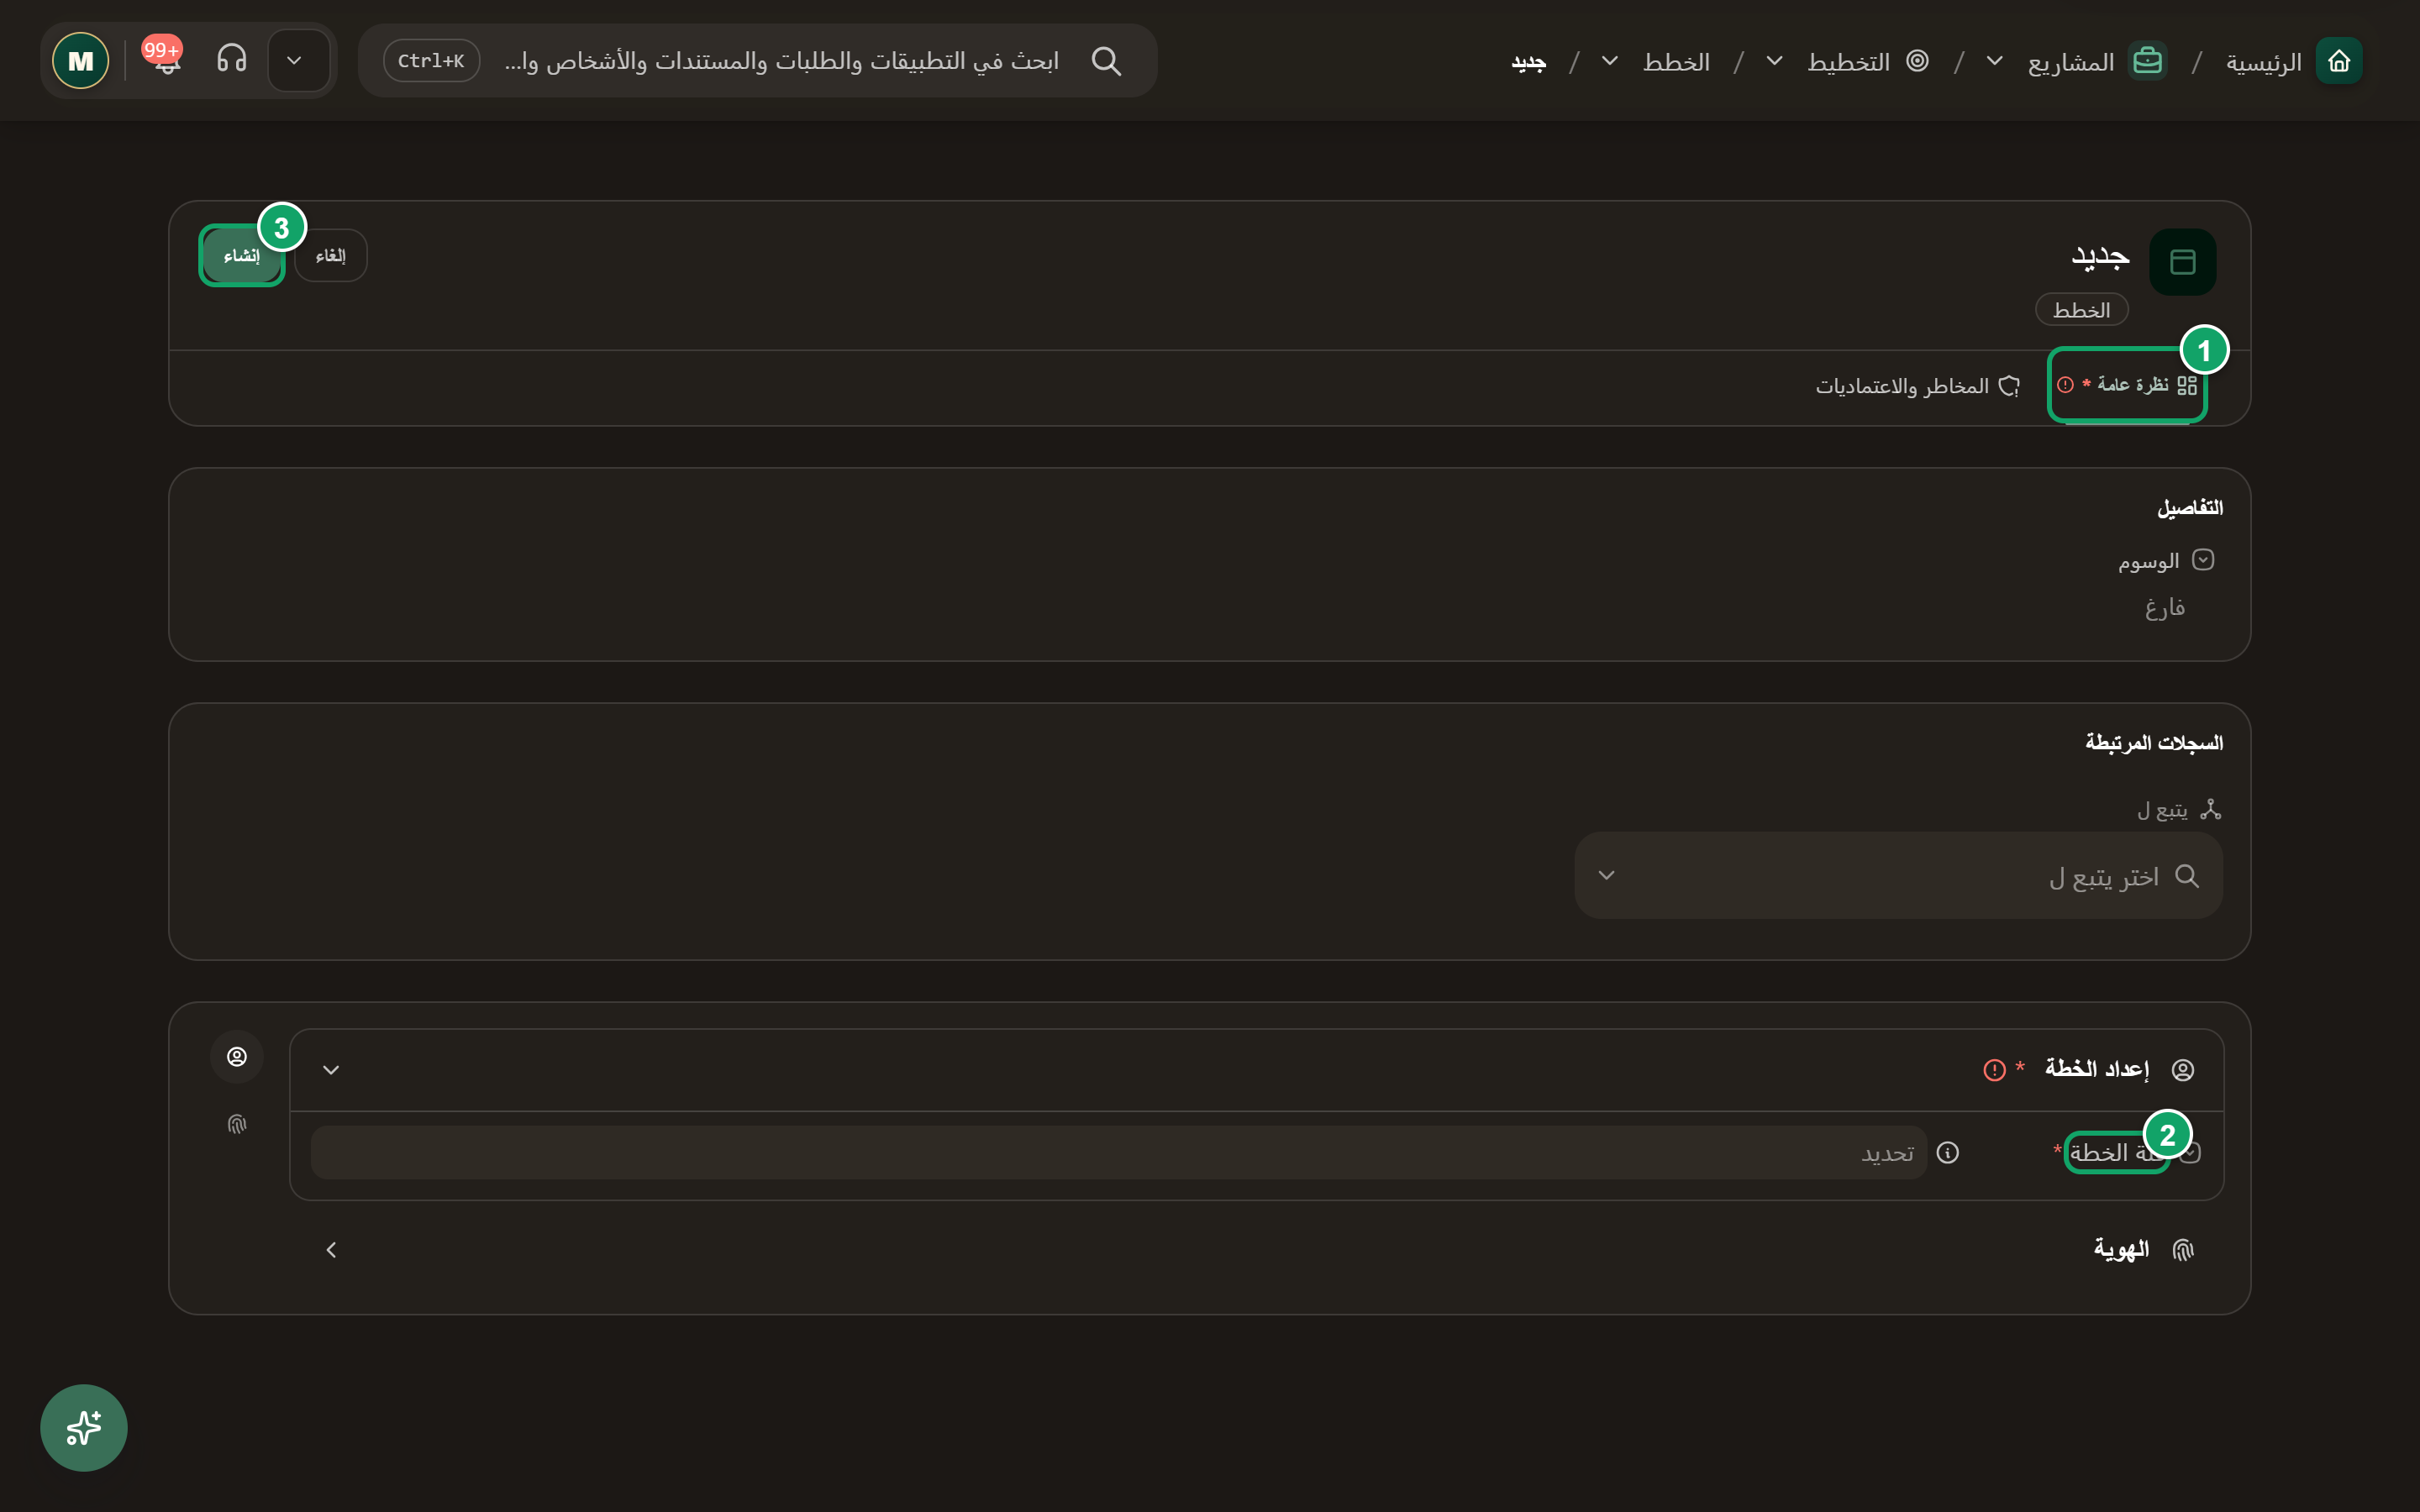
\includegraphics[width=0.95\linewidth,height=0.72\textheight,keepaspectratio]{figures/screens/ch05-plans-ar.png}
\caption{بداية إنشاء خطة قبل اختيار فئتها}
\label{fig:projects-screen-plans}
\shotnote{يبدأ النموذج بحقل «فئة الخطة»، ثم تظهر الاختيارات المناسبة للفئة. لذلك لا تتوقع رؤية جميع بيانات الخطة أو تبويباتها قبل تحديد ما تريد التخطيط له؛ الصورة تعرض نموذجاً غير محفوظ. ① تبويب «نظرة عامة» الذي تبدأ منه الخطة. ② «فئة الخطة»: الحقل الإلزامي الأول، وتظهر بقية الحقول بحسبه. ③ «إنشاء»: يحفظ الخطة بعد إكمال الحقول الإلزامية.}
\end{figure}
\begin{table}[H]
\centering
\caption{ما الذي تسجّله؟}
\label{tab:projects-plans-fields}
\begin{tabularx}{\linewidth}{R{4.2cm} Y}
\rcHeaderRow
\thh{نوع البيانات} & \thh{الحقول}\\
بيانات إلزامية & «فئة الخطة».\\
بيانات إلزامية عند ظهورها & «نوع الخطة»، «الجهة المستهدفة الرئيسية»، «الإطار الأساسي»، «الاسم»، «الأولوية»، «تاريخ البدء»، «تاريخ الانتهاء»، «المالك المسؤول»، «ملف مصدر الإجراء»، «نوع القيد المالي»، «قيمة الغلاف المالي»، «عملة الغلاف المالي»، «رابط الميزانية الإلزامي»، «التفويض»، «منطق الخدمة / عبء العمل»، «منهج تخطيط عبء العمل»، «تاريخ السريان»، «الاختصاص / التغطية»، «نوع السياسة»، «مستوى الإلزام». يعتمد ظهورها على نوع السجل وإعداداته.\\
بيانات إضافية & «الأطر الإضافية»، «الحالة»، «الوصف»، «الأفق التخطيطي»، «وتيرة المراجعة»، «المطّلع»، «الراعي»، «الجهة الحاكمة»، «الوحدة المسؤولة»، «مسؤول المراجعة»، «عقد التغطية»، «مواقع التغطية»، «دورة الخطة»، «جهات النطاق»، «الخطة المرجعية»، «الهدف المرتبط»، «المبادرة المرتبطة»، «السنة المالية»، «حالة التوقع»، «معايير النجاح»، «تاريخ الانتهاء»، «يحل محل الخطة»، «معايير الفاعلية»، «ملاحظات التخطيط»، «الوسوم».\\
نتائج يحسبها النظام & «فئة الجهة المستهدفة»، «حالة الصحة»، «ملخص خط الأساس»، «إصدار خط الأساس»، «الإصدار»، «حالة المراجعة»، «يتطلب اعتماداً»، «مرحلة الاعتماد»، «حالة الاعتماد»، «آخر مراجعة في»، «المراجعة القادمة في»، «إشارة إعادة خط الأساس»، «سبب إعادة خط الأساس»، «الجهد المخطط للموارد (ساعات)»، «الجهد الفعلي للموارد (ساعات)»، «ملخص التكلفة المخططة للموارد»، «السعة المخططة للموارد (ساعات)»، «التكلفة المخططة للموارد»، «التكلفة الملتزم بها للموارد»، «ملخص التكلفة الفعلية للموارد»، «التكلفة الفعلية للموارد»، «انحراف تكلفة الموارد»، «ملخص كميات الموارد»، «الكمية المخططة للموارد»، «الكمية الفعلية للموارد»، «نسبة استخدام سعة الموارد \%»، «عدد المخاطر المفتوحة»، «عدد الاعتماديات المعطلة»، «نسبة تغطية المعالجات»، «إجمالي التعرض الكامن»، «إجمالي التعرض المتبقي»، «نسبة تغطية السيناريوهات»، «نسبة اكتمال تحليل الأثر»، «نسبة جاهزية الإجراءات»، «نسبة نجاح التمارين»، «نسبة تغطية الضوابط»، «عدد الملاحظات المفتوحة»، «عدد الحوادث النشطة»، «نسبة التقدم»، «مرحلة حالة الخطة»، «مفتاح ملف الخطة»، «قالب حالة الخطة». راجع بياناتها المصدرية عند اختلاف النتيجة المتوقعة.\\
\end{tabularx}
\end{table}
\begin{table}[H]
\centering
\caption{التبويبات والسجلات المرتبطة}
\label{tab:projects-plans-tabs}
\begin{tabularx}{\linewidth}{R{4.2cm} Y}
\rcHeaderRow
\thh{التبويب} & \thh{ما الذي تجده فيه؟}\\
«نظرة عامة» & «إعداد الخطة»؛ «الهوية»؛ «الملكية والمساءلة»؛ «الحوكمة»؛ «الجدول الزمني»؛ «الغلاف المالي»؛ «التفويض وحجم العمل»\\
«المصدر» & «مصدر الإجراء والمواءمة»\\
«المعالم» & يعرض المعلومات المرتبطة بهذا الجانب عندما تنطبق إعدادات السجل.\\
«التنفيذ» & «سجل التنفيذ»؛ «حزم العمل»؛ «مسارات حزم العمل»؛ «المخرجات»؛ «نموذج المعالم»؛ «سجل المعالم»؛ «المشكلات والعوائق»؛ «التصعيدات»؛ «التزامات الخدمة»؛ «قياسات الخدمة»؛ «إخلالات الخدمة»؛ «إجراءات الاستعادة»؛ «طلبات التغيير»؛ «مراجعات البوابة»؛ معالم التخطيط (\ref{sec:projects-feature-planning-milestones})؛ هيكل العمل / حزم العمل (\ref{sec:projects-feature-wbs-items})؛ المخرجات / المنتجات (\ref{sec:projects-feature-deliverables})\\
«المواءمة» & «روابط الهرمية والمواءمة»\\
«التغطية» & «التغطية»\\
«النطاق» & «الجهة المستهدفة الأساسية»؛ «النطاق الإضافي»\\
«الإطار» & «نموذج الإطار»؛ «المحاور الاستراتيجية»؛ «الأهداف»؛ «مقاييس بطاقة الأداء»؛ «خريطة الاستراتيجية»؛ «دورات OKR»؛ «النتائج الرئيسية»؛ «مسارات المراجعات»؛ «مواءمة هوشين»؛ «مصفوفة X / كاتشبول»؛ «النماذج المنطقية»؛ «عناصر مسار التغيير»؛ «سلسلة النتائج»؛ «السياق / الجهات / المسار السببي»؛ «دورة حياة السياسة»؛ «تدابير السياسة»؛ «نموذج خارطة الطريق»؛ «عناصر خارطة الطريق»؛ «مسارات الأهداف»؛ المحاور التخطيطية (\ref{sec:projects-feature-planning-themes})؛ أهداف التخطيط (\ref{sec:projects-feature-planning-objectives})؛ دورات OKR (\ref{sec:projects-feature-planning-okrs})؛ النتائج الرئيسية (\ref{sec:projects-feature-planning-key-results})؛ متابعات النتائج الرئيسية (\ref{sec:projects-feature-planning-key-result-checkins})؛ عناصر هوشين (\ref{sec:projects-feature-planning-hoshin-items})؛ روابط مصفوفة X لهوشين (\ref{sec:projects-feature-planning-hoshin-x-matrix-links})؛ تبادلات كاتشبّول لهوشين (\ref{sec:projects-feature-planning-hoshin-catchball-exchanges})؛ الإجراءات المضادة لهوشين (\ref{sec:projects-feature-planning-hoshin-countermeasures})؛ نظرية التغيير (\ref{sec:projects-feature-theory-of-change})؛ أطر النتائج (\ref{sec:projects-feature-logframes})؛ أهداف الإطار المنطقي (\ref{sec:projects-feature-logframe-goals})؛ نتائج الإطار المنطقي (\ref{sec:projects-feature-logframe-outcomes})؛ مخرجات الإطار المنطقي (\ref{sec:projects-feature-logframe-outputs})؛ أنشطة الإطار المنطقي (\ref{sec:projects-feature-logframe-activities})\\
«المبادرات» & «المبادرات الأصلية»؛ المبادرات التخطيطية (\ref{sec:projects-feature-planning-initiatives})\\
«المخرجات» & يعرض المعلومات المرتبطة بهذا الجانب عندما تنطبق إعدادات السجل.\\
«الحوكمة» & «اعتمادات دورة الحياة»؛ «جدولة المراجعة»؛ «المراجعات الحوكمية»؛ «القرارات»؛ «سجل التغييرات»؛ «الإصدارات وخطوط الأساس»؛ مراجعات التخطيط (\ref{sec:projects-feature-planning-reviews})؛ اعتمادات التخطيط (\ref{sec:projects-feature-planning-approvals})؛ قرارات التخطيط (\ref{sec:projects-feature-planning-decisions})\\
«الميزانية» & «نموذج الميزانية»؛ «الميزانيات»؛ «بنود الميزانية»؛ «فترات الميزانية»؛ الميزانيات (\ref{sec:projects-feature-budgets})؛ بنود الميزانية (\ref{sec:projects-feature-budget-lines})؛ فترات بند الميزانية (\ref{sec:projects-feature-budget-line-periods})\\
«التمويل» & «نموذج التمويل»؛ «مصادر التمويل»؛ مصادر التمويل (\ref{sec:projects-feature-funding-sources})\\
«القوى العاملة» & «نموذج القوى العاملة»؛ «احتياجات التوظيف»؛ «المناصب»؛ «التعيينات»\\
«التوظيف» & «نموذج التوظيف»؛ «الشواغر»\\
«المشتريات» & «نموذج المشتريات»؛ «المشتريات»؛ المشتريات (\ref{sec:projects-feature-procurements})\\
«العقود» & «نموذج العقود»\\
«الطلب والسعة» & «نموذج الطلب والسعة»\\
«التخصيصات» & «نموذج التخصيص»؛ «تخصيصات السعة»\\
«المسار» & «مسار جمع التمويل»؛ «الفرص»\\
«المنح والالتزامات» & «المنح والقيود»\\
«الأصول» & «نموذج سجل الأصول»؛ «سجل الأصول»\\
«دورة الحياة» & «نموذج دورة الحياة»؛ «أحداث دورة الحياة»\\
«البوابات» & يعرض المعلومات المرتبطة بهذا الجانب عندما تنطبق إعدادات السجل.\\
«التصعيدات» & يعرض المعلومات المرتبطة بهذا الجانب عندما تنطبق إعدادات السجل.\\
«ضبط التغيير» & يعرض المعلومات المرتبطة بهذا الجانب عندما تنطبق إعدادات السجل.\\
«الموارد» & «نموذج الموارد»؛ «سجل الموارد»؛ موارد التخطيط (\ref{sec:projects-feature-planning-resources})؛ تخصيص الموارد (\ref{sec:projects-feature-resource-allocations})\\
«المخاطر والاعتماديات» & «نموذج المخاطر»؛ «المخاطر»؛ «الاعتماديات»؛ اعتماديات التخطيط (\ref{sec:projects-feature-planning-dependencies})؛ سجل المخاطر (\ref{sec:projects-feature-planning-risks})\\
«الأداء» & «نموذج الأداء»؛ «الأهداف المرحلية»؛ «المؤشرات»؛ «قياسات المؤشرات»؛ «مسارات القياسات»؛ مؤشرات الأداء (\ref{sec:projects-feature-performance-indicators})؛ الأهداف المرحلية (\ref{sec:projects-feature-planning-time-targets})\\
«البيانات» & «مصادر البيانات»؛ «بروتوكولات المؤشرات»؛ «فترات التقارير»؛ «مراجعات جودة البيانات»؛ «سجل الأدلة»؛ فترات التقارير (\ref{sec:projects-feature-planning-reporting-periods})؛ مصادر بيانات التخطيط (\ref{sec:projects-feature-planning-data-sources})؛ عناصر الأدلة (\ref{sec:projects-feature-planning-evidence-items})\\
«التقييم» & «أسئلة التقييم»؛ «نتائج التقييم»؛ «استجابات الإدارة»؛ أسئلة التقييم (\ref{sec:projects-feature-planning-evaluation-questions})؛ نتائج التقييم (\ref{sec:projects-feature-planning-evaluation-findings})؛ استجابات الإدارة (\ref{sec:projects-feature-planning-management-responses})\\
«التعلم» & «أجندة التعلم»؛ «رؤى التعلم»؛ بنود أجندة التعلم (\ref{sec:projects-feature-planning-learning-agenda-items})؛ رؤى التعلم (\ref{sec:projects-feature-planning-learning-insights})\\
«التحسين» & «فرص التحسين»؛ فرص التحسين (\ref{sec:projects-feature-planning-improvement-opportunities})\\
«الافتراضات» & «الافتراضات»؛ «سجل الافتراضات»؛ افتراضات التخطيط (\ref{sec:projects-feature-planning-assumptions})\\
«الدورة» & «نموذج الدورة»\\
«المشاورات» & «سجل المشاورات»\\
«النشر» & «الإصدارات»\\
«الالتزامات» & يعرض المعلومات المرتبطة بهذا الجانب عندما تنطبق إعدادات السجل.\\
«القياسات» & يعرض المعلومات المرتبطة بهذا الجانب عندما تنطبق إعدادات السجل.\\
«الإخلالات» & يعرض المعلومات المرتبطة بهذا الجانب عندما تنطبق إعدادات السجل.\\
«الاستعادة» & «أهداف التعافي»؛ «نطاق التعافي»؛ «تسلسل الاستعادة والتحويل»\\
«الضوابط» & «نموذج الضوابط»؛ «سجل الضوابط»؛ ضوابط التخطيط (\ref{sec:projects-feature-planning-controls})\\
«التقييمات» & «تقييمات الضوابط»؛ تقييمات الضوابط (\ref{sec:projects-feature-planning-control-assessments})\\
«الملاحظات» & «سجل الملاحظات»؛ «الإقرارات واعتمادات الإغلاق»؛ ملاحظات التخطيط (\ref{sec:projects-feature-planning-findings})\\
«الحوادث» & «سجل الحوادث»؛ «الخطورة والتصنيف»؛ حوادث التخطيط (\ref{sec:projects-feature-planning-incidents})\\
«الخط الزمني» & «الخط الزمني للحادث»؛ أحداث الخط الزمني للحوادث (\ref{sec:projects-feature-planning-incident-events})\\
«ما بعد الحادث» & «مراجعة ما بعد الحادث»\\
«السيناريوهات» & «سجل السيناريوهات»؛ «مصفوفة المحفزات»؛ «معايير التفعيل»؛ سيناريوهات التخطيط (\ref{sec:projects-feature-planning-scenarios})\\
«الكتب التشغيلية» & «نموذج الكتب التشغيلية»\\
«تحليل أثر الأعمال» & «نموذج تحليل الأثر»؛ «سجل تحليل الأثر»؛ سجلات تحليل أثر الأعمال (\ref{sec:projects-feature-planning-bia-entries})\\
«الاستمرارية» & «استراتيجيات الاستمرارية»؛ «الحلول اليدوية البديلة»\\
«الإجراءات» & «الإجراءات والكتب التشغيلية»؛ إجراءات التخطيط (\ref{sec:projects-feature-planning-procedures})\\
«التمارين» & «التمارين والاختبارات»؛ تمارين التخطيط (\ref{sec:projects-feature-planning-exercises})\\
«الاختبارات» & «برنامج اختبارات التعافي»\\
\end{tabularx}
\end{table}
\begin{figure}[H]
\centering
\begin{tikzpicture}[node distance=0.5cm]
\node[stepBox] (n0) {\RL{اختيار صفحة العمل}};
\node[stepBox,below=of n0] (n1) {\RL{الخطط}};
\node[stepBox,below=of n1] (n2) {\RL{الحفظ ثم إعادة الفتح}};
\draw[flowsTo] (n0) -- (n1);
\draw[flowsTo] (n1) -- (n2);
\end{tikzpicture}
\rclegend
\caption{مسار العمل والتحقق}
\label{fig:projects-plans-flow}
\shotnote{يبدأ العمل بفتح «الخطط» واختيار السجل الصحيح قبل إدخال التفاصيل. إعادة فتحه بعد الحفظ تؤكد بقاء البيانات، لكنها لا تعني اعتمادها أو اكتمال العمل المرتبط بها.}
\end{figure}

\subsection{خطوات العمل والتحقق}
\begin{enumerate}
\item افتح «الخطط» من تطبيق «المشاريع»، ثم اضغط «إضافة». اختر «فئة الخطة» أولاً، ثم النوع المتاح الذي يطابق العمل المطلوب.
\item اختر «الجهة المستهدفة الرئيسية» من السجلات المتاحة، ثم «الإطار الأساسي». أكمل الاسم والمالك المسؤول والأولوية وتاريخي البدء والانتهاء، ثم راجع أي حقول إضافية يطلبها النوع المختار.
\item اضغط «إنشاء»، ثم أعد فتح الخطة. تحقق من الجهة والمالك والفترة، وافتح الأقسام المتاحة لإضافة الأهداف أو التنفيذ أو القياس حسب نوعها.
\item راجع مرحلة الخطة قبل تعديلها؛ فقد لا تسمح المرحلة الحالية بتغيير الإعدادات أو إضافة بعض السجلات. عالج رسالة التحقق أو اطلب مراجعة الصلاحية بدلاً من تكرار الخطة.
\end{enumerate}

\textbf{تطبيق المثال:} في المثال الافتراضي، استخدم «خطة تحسين جاهزية فرع حلب» في «الاسم»، ثم أكمل بقية البيانات بما يناسب عمل الأفق. لا تستخدم قيم المثال بديلاً عن السجلات الفعلية المطلوبة في حقول الربط.

\textbf{تحقق ومعالجة المشكلة:} يجب أن تجد السجل بعد إعادة فتحه وأن تبقى البيانات التي حفظتها. إذا لم يظهر، فراجع البحث والفلاتر والنطاق وصلاحية الوصول قبل إنشائه مرة أخرى. وإذا تعذر الحفظ، فأكمل الحقول المطلوبة ورسائل التحقق؛ أما غياب تبويب أو قفل حقل فيستدعي مراجعة نوع السجل وإطاره ومرحلته مع المسؤول.

\clearpage
\section{المشاريع}
\label{sec:projects-feature-projects}

يجمع المشروع عملاً محدد النطاق له مدير ونتيجة مطلوبة. ابدأ بتعريفه وميثاقه، ثم استخدم الأقسام المتاحة لتخطيط التنفيذ ومراجعة التقدم.

\begin{rcnote}[مثال: شركة الأفق]
تنشئ سارة مشروع «تجهيز زيارة فرع حلب» بالرمز \en{HZN-PRJ-01}، وتحدّد النتيجة المطلوبة في الميثاق. يتولى عمر إعداد ملف الزيارة بعد تحديد مسؤوليته، وتراجع سارة المخرج عند التسليم.
\end{rcnote}

\textbf{المسار ومن يستخدمه:} افتح تطبيق «المشاريع»، ثم بطاقة «المشاريع». هذه صفحة رئيسية في التطبيق. يستخدمها المسؤول عن هذا العمل، ويعدّل الموظف البيانات المسموح له بها وفق صلاحياته.

\subsection{الميثاق يسبق التخطيط التفصيلي}
يجمع تبويب «ميثاق المشروع» الغرض والأهداف ومعايير النجاح والنطاق وما يقع خارجه، ودراسة الجدوى والافتراضات والمخاطر وبيانات الاعتماد. راجع «مدير المشروع» و«الراعي» والتواريخ، ولا تعتبر حفظ السجل اعتماداً للميثاق.

يتطلب ظهور أقسام التخطيط أن تكون «حالة الميثاق» معتمدة وأن يتجاوز المشروع مرحلة الإعداد. ويحدد «الإطار المنهجي» و«نهج التسليم» ما يظهر من مراحل وسباقات وحوكمة، بينما تؤثر طبيعة المشروع والعميل في المشتريات والمتابعة والتقييم. بعد الاعتماد قد تُقفل بيانات الإعداد، ويُراجع تعديلها عبر ضبط التغيير.

\textbf{التقدم والحالة:} تُحسب نسبة التقدم من سجلات التنفيذ ذات الصلة. راجع حزم العمل والمخرجات والمؤشرات قبل تفسير حالة المشروع؛ ولا تخلط اكتمال مهمة منفردة باكتمال المشروع كله.
\begin{figure}[H]
\centering
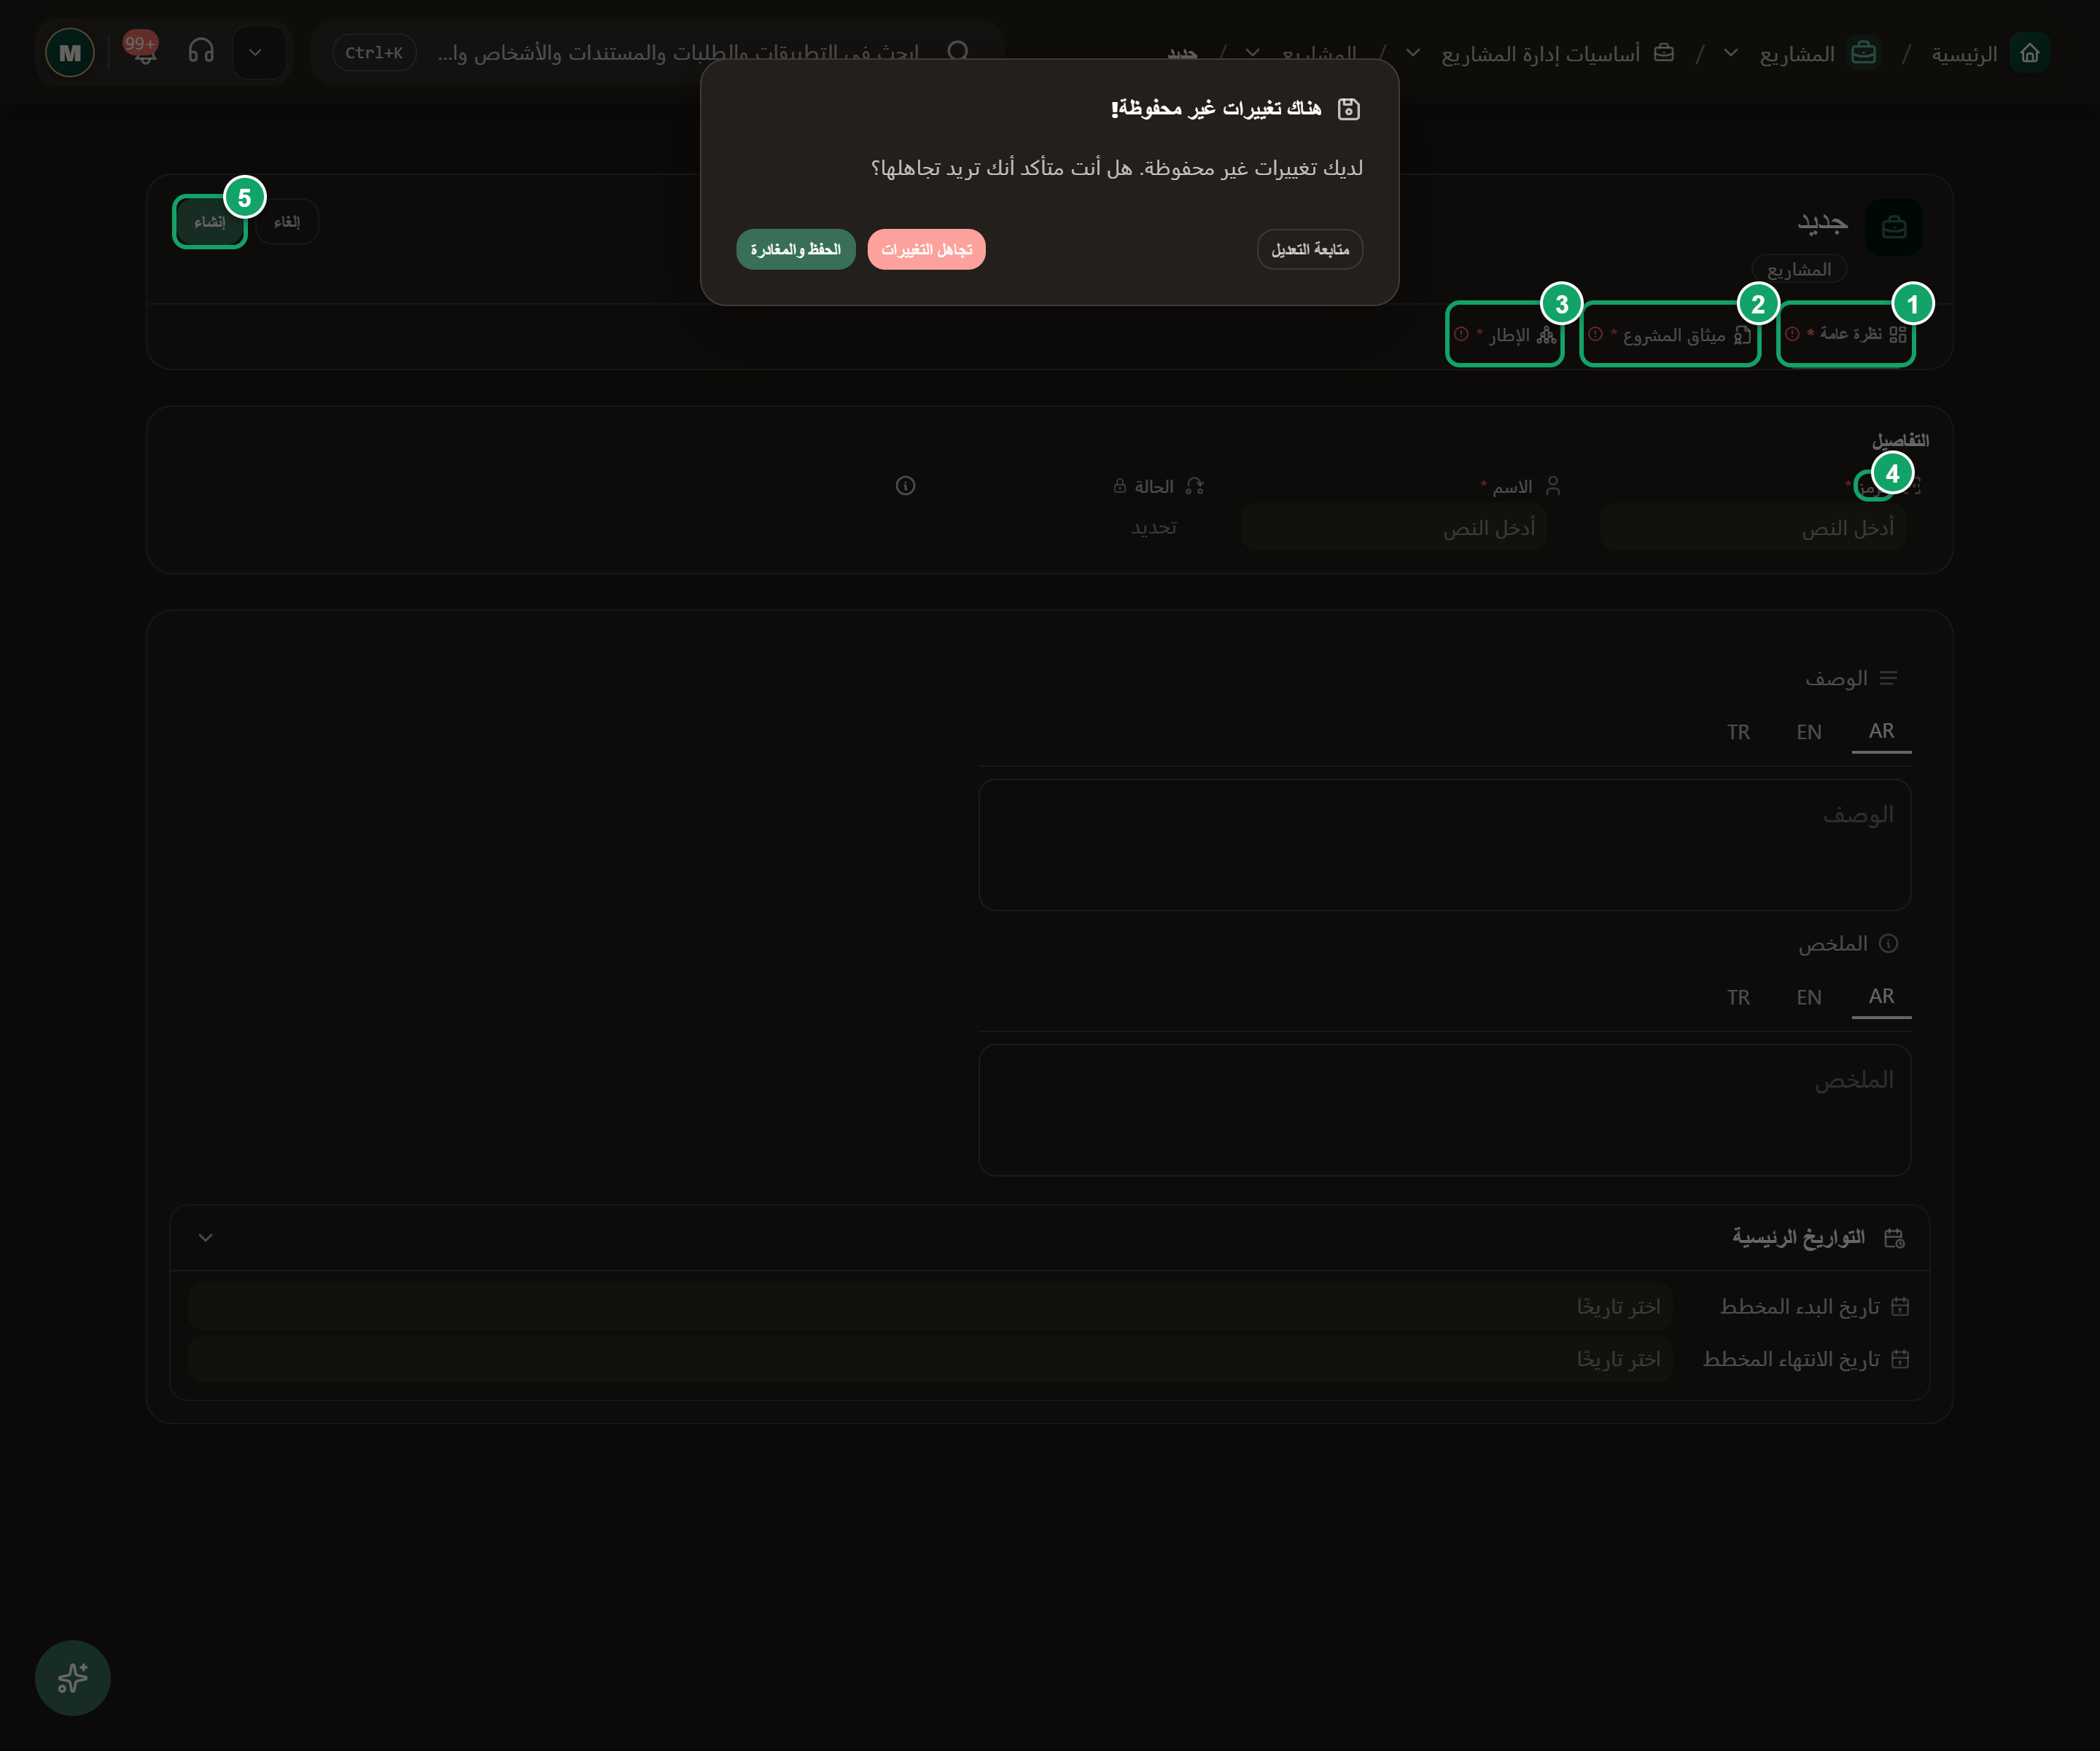
\includegraphics[width=0.95\linewidth,height=0.72\textheight,keepaspectratio]{figures/screens/ch05-project-create-ar.png}
\caption{نظرة عامة على مشروع جديد غير محفوظ}
\label{fig:projects-screen-project-create}
\shotnote{يجمع هذا التبويب هوية المشروع ووصفه وتواريخه المخططة. ظهور الاسم والرمز لا يكفي لإكمال الإنشاء؛ يطلب التبويبان الآخران بيانات الميثاق والإطار، وتبقى حالة المشروع مرتبطة بإعداداته. ① تبويب «نظرة عامة». ② تبويب «ميثاق المشروع». ③ تبويب «الإطار»؛ وتعني العلامة الحمراء أن في التبويب حقلاً إلزامياً فارغاً. ④ «الرمز»: أول الحقول الإلزامية. ⑤ «إنشاء».}
\end{figure}
\begin{figure}[H]
\centering
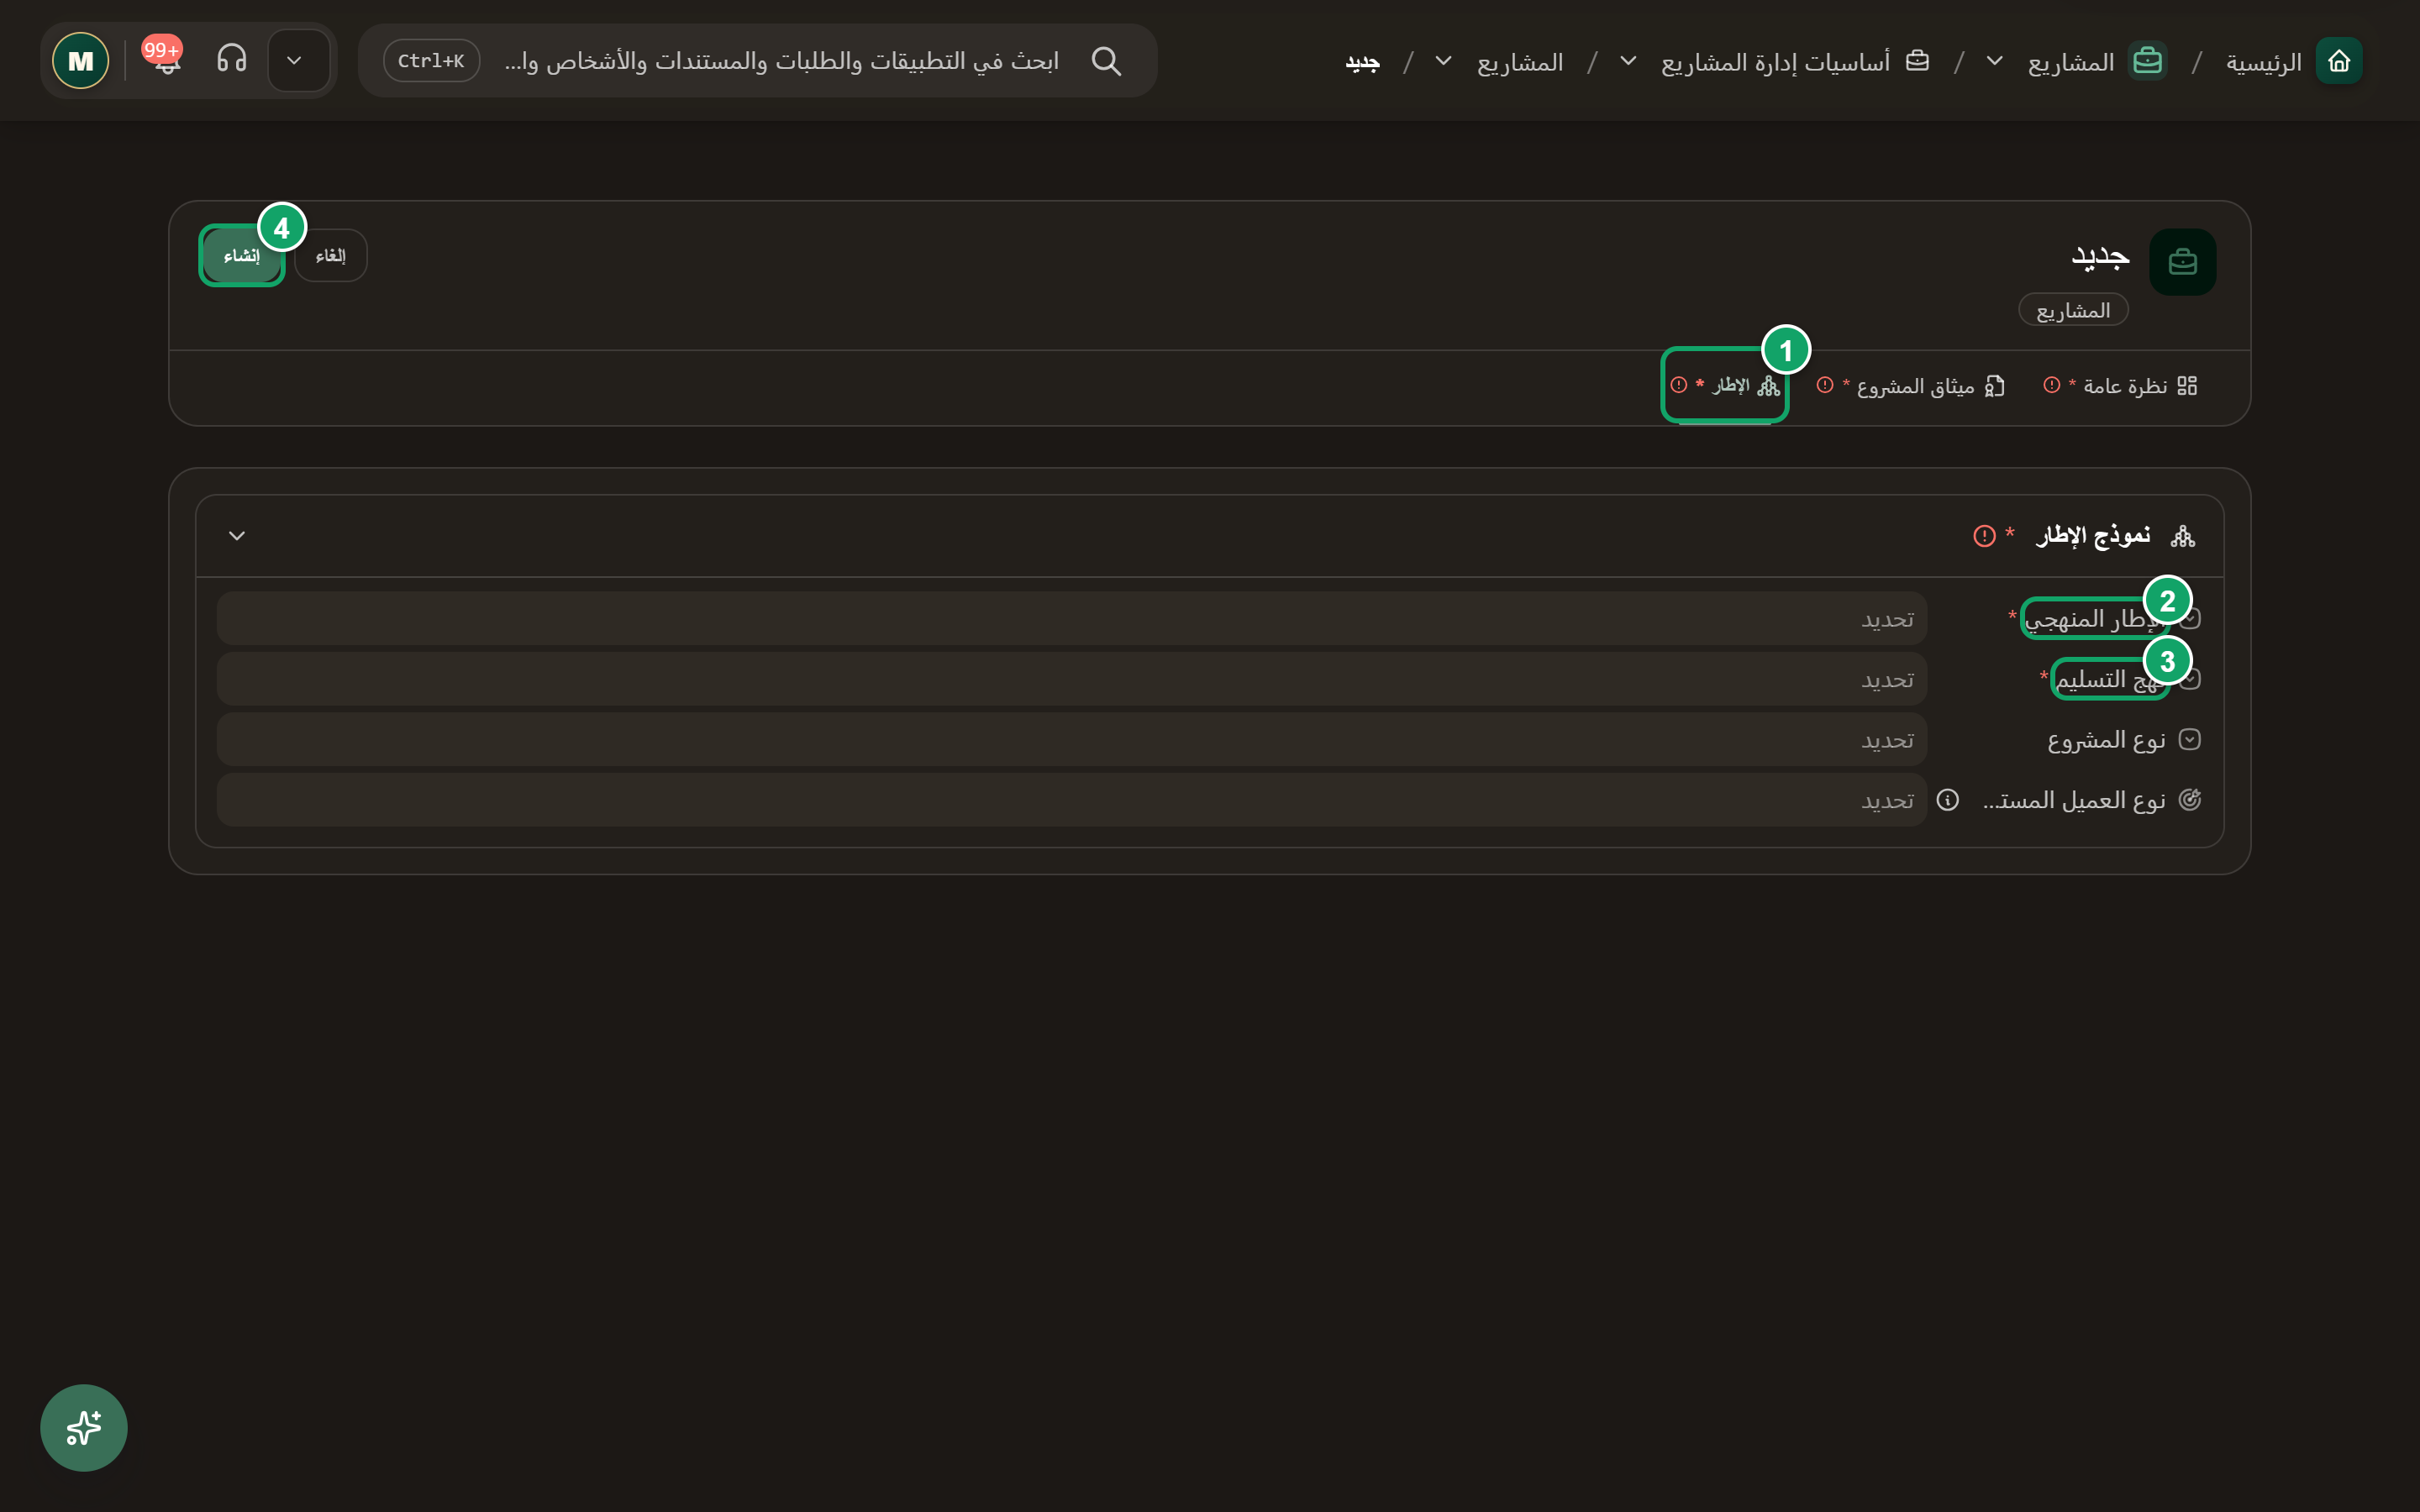
\includegraphics[width=0.95\linewidth,height=0.72\textheight,keepaspectratio]{figures/screens/ch05-project-framework-ar.png}
\caption{اختيار إطار المشروع ونهج التسليم}
\label{fig:projects-screen-project-framework}
\shotnote{يحدد «الإطار المنهجي» و«نهج التسليم» طريقة تنظيم المشروع والأقسام المناسبة له. راجع أيضاً نوع المشروع والعميل المستهدف، لأنهما يساعدان على تحديد الحاجة إلى المشتريات والمتابعة؛ النموذج في الصورة لم يُحفظ. ① تبويب «الإطار». ② «الإطار المنهجي»: الطريقة التي يُدار بها المشروع. ③ «نهج التسليم»: كيف تُسلَّم النتائج. ④ «إنشاء»: يحفظ المشروع بعد إكمال التبويبات الإلزامية.}
\end{figure}
\begin{figure}[H]
\centering
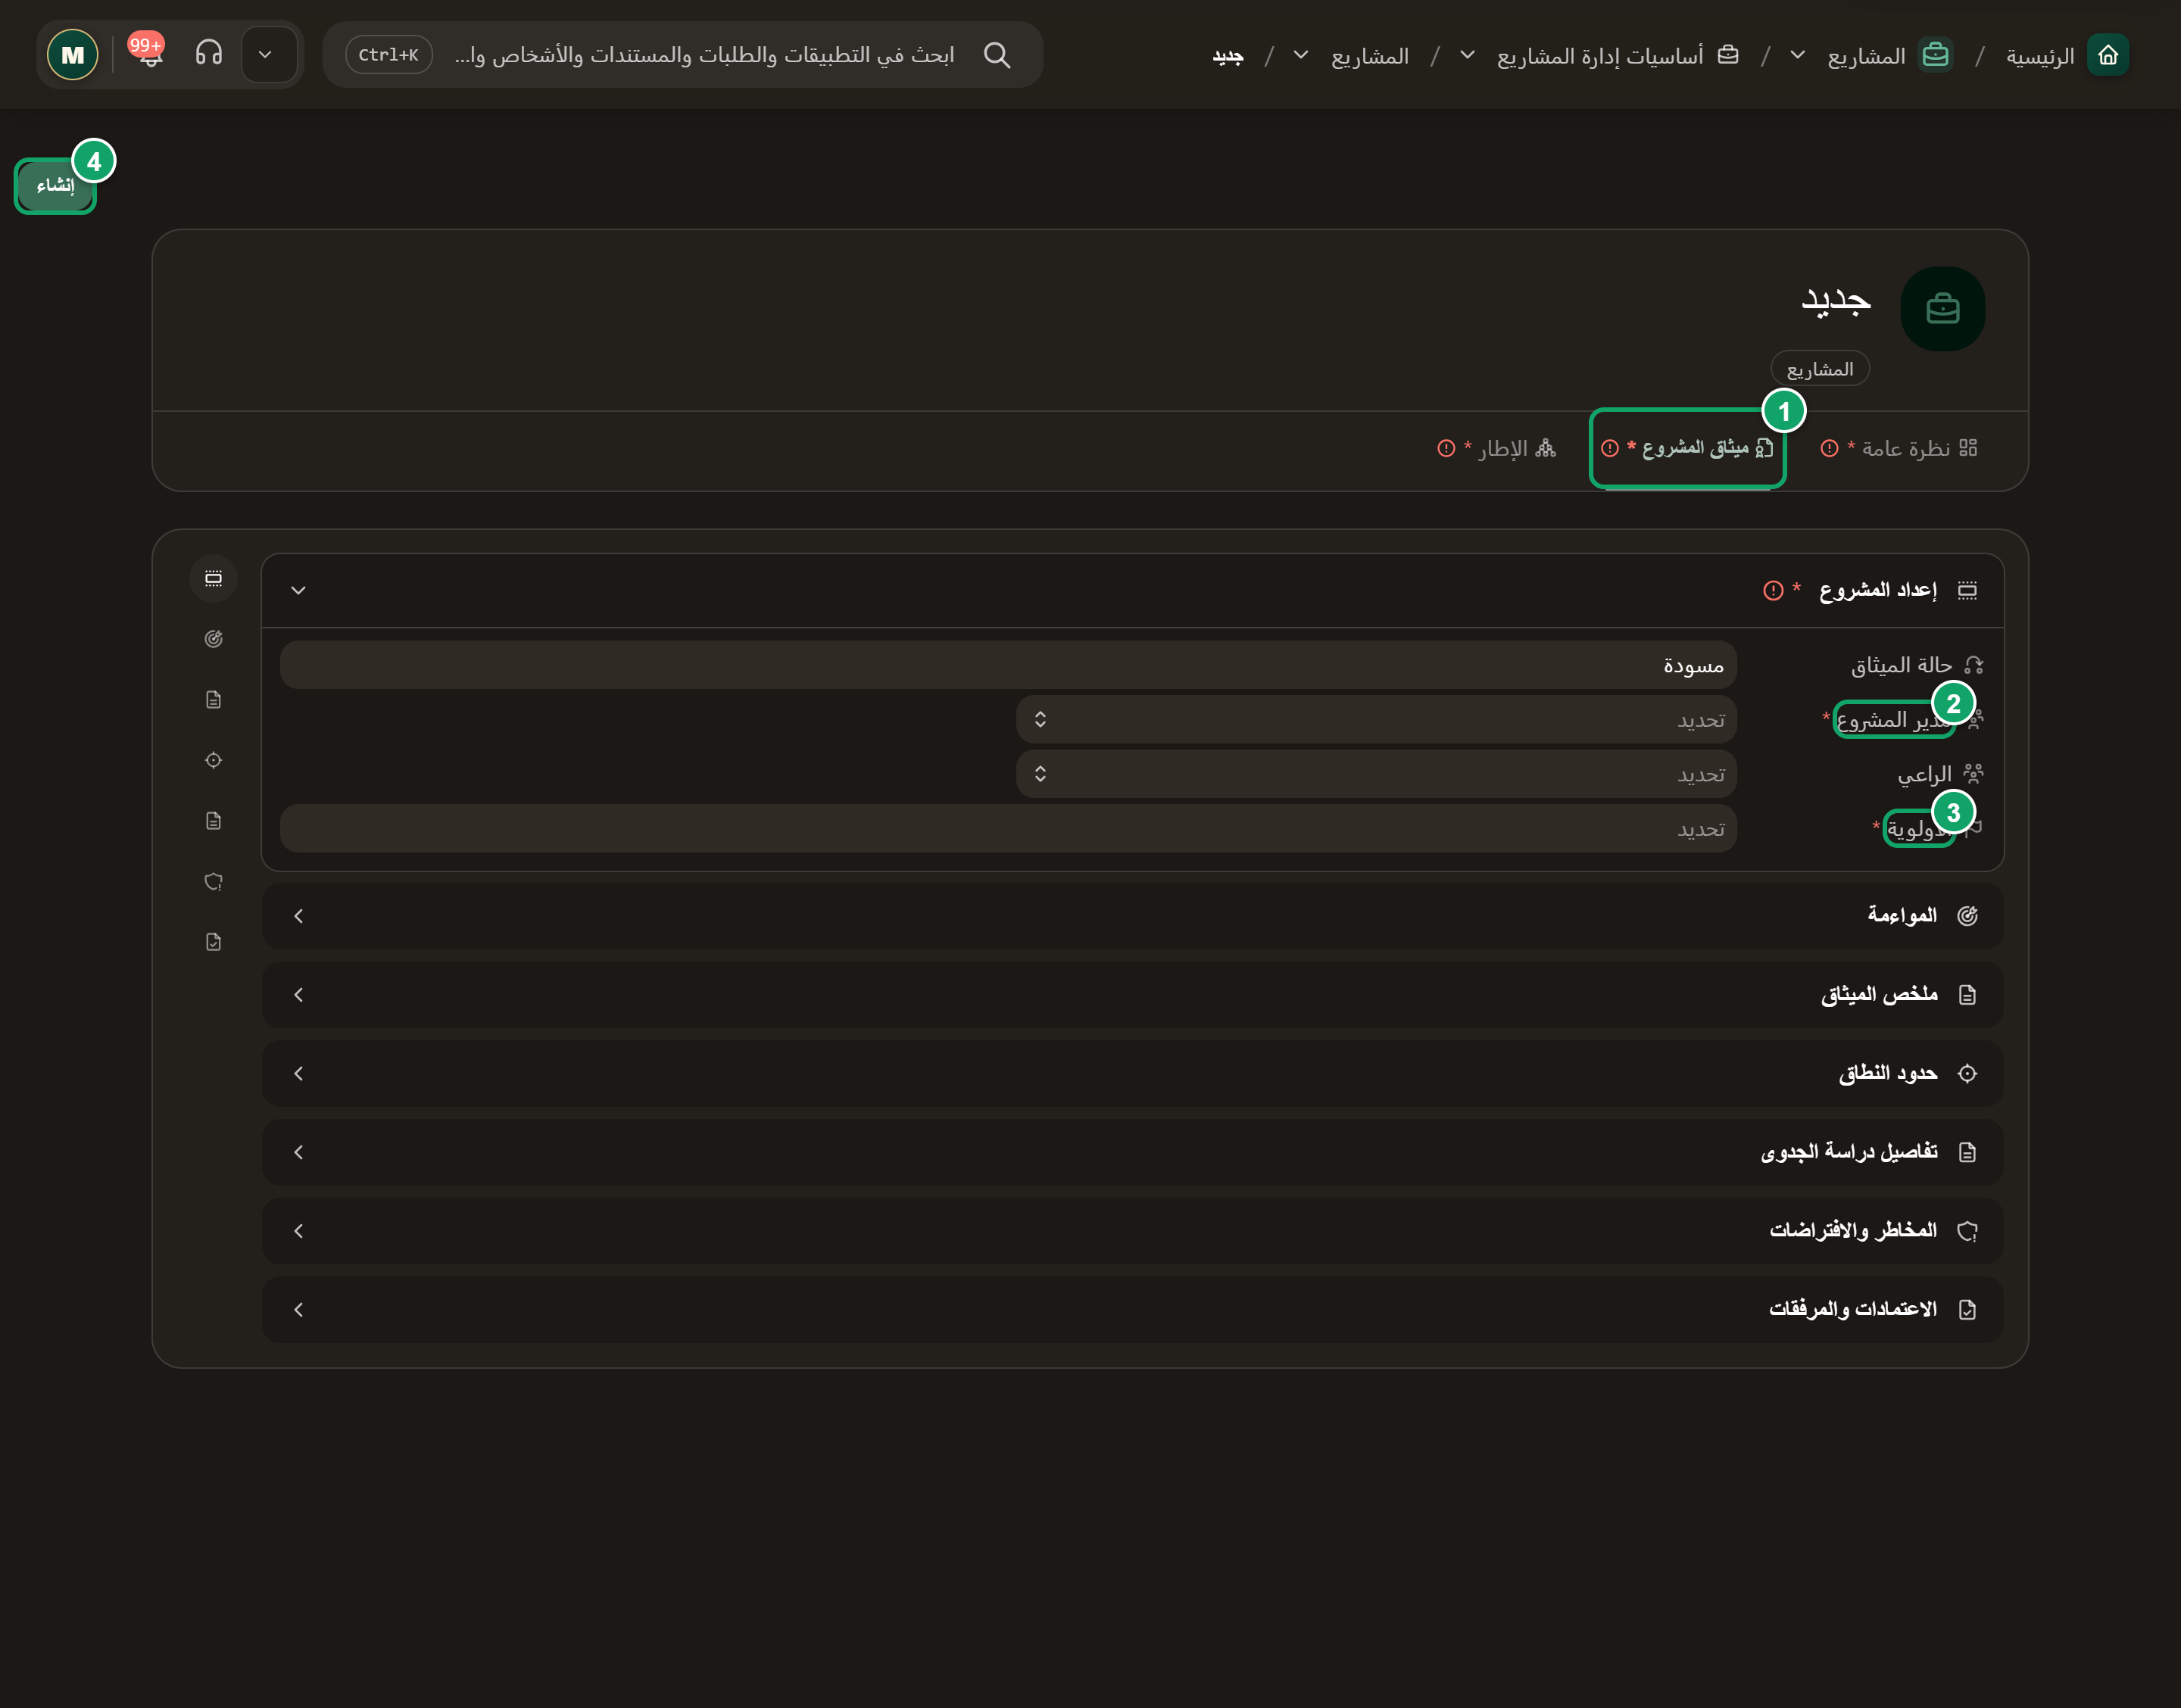
\includegraphics[width=0.95\linewidth,height=0.72\textheight,keepaspectratio]{figures/screens/ch05-project-charter-ar.png}
\caption{إعداد المشروع وأقسام الميثاق}
\label{fig:projects-screen-project-charter}
\shotnote{يظهر الميثاق بحالة «مسودة»، مع اختيار مدير المشروع والراعي والأولوية. تجمع الأقسام الأخرى الغرض والنطاق ودراسة الجدوى والمخاطر والاعتماد؛ فتح التبويب أو حفظ بياناته لا يعني أن الميثاق اعتُمد. ① تبويب «ميثاق المشروع». ② «مدير المشروع». ③ «الأولوية». ④ «إنشاء».}
\end{figure}
\begin{table}[H]
\centering
\caption{ما الذي تسجّله؟}
\label{tab:projects-projects-fields}
\begin{tabularx}{\linewidth}{R{4.2cm} Y}
\rcHeaderRow
\thh{نوع البيانات} & \thh{الحقول}\\
بيانات إلزامية & «الرمز»، «الاسم»، «الإطار المنهجي»، «نهج التسليم»، «مدير المشروع»، «الأولوية».\\
بيانات إضافية & «الوصف»، «نوع المشروع»، «نوع العميل المستهدف»، «الحالة»، «حالة الميثاق»، «عنوان الميثاق»، «الغرض»، «الأهداف»، «معايير النجاح»، «وصف النطاق»، «خارج النطاق»، «نوع دراسة الجدوى»، «التوافق الاستراتيجي»، «الفوائد المتوقعة»، «تأثير أصحاب المصلحة»، «العائد المتوقع»، «الميزانية المقدرة»، «المدة المقدرة (أيام)»، «تاريخ البدء المستهدف»، «تاريخ الانتهاء المستهدف»، «الافتراضات الرئيسية»، «القيود الرئيسية»، «المخاطر الرئيسية»، «اعتمد بواسطة»، «تاريخ الاعتماد»، «المرفقات»، «المحفظة»، «البرنامج»، «الخطط»، «الراعي»، «المالكون»، «المطّلعون»، «تجاوز صحة النطاق»، «تجاوز صحة الجودة»، «تاريخ البدء المخطط»، «تاريخ الانتهاء المخطط»، «تاريخ البدء الفعلي»، «تاريخ الانتهاء الفعلي»، «المرحلة الحالية»، «العملة»، «الميزانية المخططة»، «التكلفة الفعلية»، «القيمة المكتسبة»، «القيمة المخططة»، «القطاع»، «المانحون»، «الإطار المنطقي»، «الوسوم».\\
نتائج يحسبها النظام & «قالب حالة المشروع»، «مرحلة الإعداد»، «ملف الإعداد»، «اكتمل الإعداد»، «الحوكمة مطلوبة»، «الصحة العامة»، «صحة النطاق»، «صحة الجدول الزمني»، «صحة التكلفة»، «صحة الجودة»، «صحة المخاطر»، «مؤشر أداء التكلفة»، «مؤشر أداء الجدول الزمني»، «نسبة التقدم». راجع بياناتها المصدرية عند اختلاف النتيجة المتوقعة.\\
\end{tabularx}
\end{table}
\begin{table}[H]
\centering
\caption{التبويبات والسجلات المرتبطة}
\label{tab:projects-projects-tabs}
\begin{tabularx}{\linewidth}{R{4.2cm} Y}
\rcHeaderRow
\thh{التبويب} & \thh{ما الذي تجده فيه؟}\\
«نظرة عامة» & «الملخص السريع»؛ «التواريخ الرئيسية»\\
«ميثاق المشروع» & «إعداد المشروع»؛ «المواءمة»؛ «ملخص الميثاق»؛ «حدود النطاق»؛ «تفاصيل دراسة الجدوى»؛ «المخاطر والافتراضات»؛ «الاعتمادات والمرفقات»\\
«الإطار» & «نموذج الإطار»؛ المحاور التخطيطية (\ref{sec:projects-feature-planning-themes})؛ أهداف التخطيط (\ref{sec:projects-feature-planning-objectives})؛ دورات OKR (\ref{sec:projects-feature-planning-okrs})؛ النتائج الرئيسية (\ref{sec:projects-feature-planning-key-results})؛ متابعات النتائج الرئيسية (\ref{sec:projects-feature-planning-key-result-checkins})؛ عناصر هوشين (\ref{sec:projects-feature-planning-hoshin-items})؛ روابط مصفوفة X لهوشين (\ref{sec:projects-feature-planning-hoshin-x-matrix-links})؛ تبادلات كاتشبّول لهوشين (\ref{sec:projects-feature-planning-hoshin-catchball-exchanges})؛ الإجراءات المضادة لهوشين (\ref{sec:projects-feature-planning-hoshin-countermeasures})؛ نظرية التغيير (\ref{sec:projects-feature-theory-of-change})؛ أطر النتائج (\ref{sec:projects-feature-logframes})؛ أهداف الإطار المنطقي (\ref{sec:projects-feature-logframe-goals})؛ نتائج الإطار المنطقي (\ref{sec:projects-feature-logframe-outcomes})؛ مخرجات الإطار المنطقي (\ref{sec:projects-feature-logframe-outputs})؛ أنشطة الإطار المنطقي (\ref{sec:projects-feature-logframe-activities})\\
«التنفيذ» & «النطاق / هيكل العمل وحزم العمل»؛ «المخرجات / المنتجات»؛ «ضبط التنفيذ»؛ «المهام / الأنشطة»؛ معالم التخطيط (\ref{sec:projects-feature-planning-milestones})؛ هيكل العمل / حزم العمل (\ref{sec:projects-feature-wbs-items})؛ المخرجات / المنتجات (\ref{sec:projects-feature-deliverables})؛ المتطلبات (\ref{sec:projects-feature-requirements})\\
«الأداء» & «مؤشرات الصحة»؛ «مسارات القياسات»؛ «المؤشرات»؛ «القياسات»؛ «بطاقة الأداء»؛ «جودة البيانات»؛ «تقارير الحالة»؛ «القيمة المكتسبة»؛ تقارير الحالة (\ref{sec:projects-feature-status-reports})؛ مؤشرات الأداء (\ref{sec:projects-feature-performance-indicators})؛ الأهداف المرحلية (\ref{sec:projects-feature-planning-time-targets})\\
«الموارد» & «القيادة»؛ «الملكية والتواصل»؛ «الفريق الأساسي»؛ «أصحاب المصلحة»؛ «مصفوفة المسؤوليات»؛ موارد التخطيط (\ref{sec:projects-feature-planning-resources})؛ أدوار الفريق (\ref{sec:projects-feature-team-roles})؛ مصفوفة المسؤوليات (\ref{sec:projects-feature-raci-entries})؛ تخصيص الموارد (\ref{sec:projects-feature-resource-allocations})؛ أصحاب المصلحة (\ref{sec:projects-feature-stakeholders})\\
«النطاق» & يعرض المعلومات المرتبطة بهذا الجانب عندما تنطبق إعدادات السجل.\\
«الجدول الزمني» & «المرحلة الحالية»؛ مراحل المشروع (\ref{sec:projects-feature-phases})؛ التبعيات (\ref{sec:projects-feature-dependencies})؛ خطوط الأساس (\ref{sec:projects-feature-baselines})\\
«المالية» & «ملخص الميزانية»؛ «تتبع التكاليف»؛ «إدارة القيمة المكتسبة»؛ المصروفات (\ref{sec:projects-feature-expenditures})\\
«الجودة» & معايير الجودة (\ref{sec:projects-feature-quality-criteria})\\
«المخاطر والمشكلات» & اعتماديات التخطيط (\ref{sec:projects-feature-planning-dependencies})؛ سجل المخاطر (\ref{sec:projects-feature-planning-risks})؛ سجل مخاطر إدارة المشاريع (\ref{sec:projects-feature-project-risks})؛ المشكلات (\ref{sec:projects-feature-issues})\\
«الاتصالات» & «خطة الاتصال»؛ خطة الاتصال (\ref{sec:projects-feature-communication-plan})\\
«المشتريات» & المشتريات (\ref{sec:projects-feature-procurements})\\
«الحوكمة» & «البيانات الوصفية»؛ مراجعات التخطيط (\ref{sec:projects-feature-planning-reviews})؛ اعتمادات التخطيط (\ref{sec:projects-feature-planning-approvals})؛ قرارات التخطيط (\ref{sec:projects-feature-planning-decisions})؛ مراجعات البوابة (\ref{sec:projects-feature-gate-reviews})؛ طلبات التغيير (\ref{sec:projects-feature-change-requests})؛ قرارات الاجتماعات (\ref{sec:projects-feature-meeting-decisions})؛ الدروس المستفادة (\ref{sec:projects-feature-lessons-learned})\\
«أجايل» & السباقات (\ref{sec:projects-feature-sprints})؛ تعريف الإنجاز (\ref{sec:projects-feature-definition-of-done})\\
«المتابعة والتقييم» & «إعداد المتابعة والتقييم»؛ المستفيدون (\ref{sec:projects-feature-beneficiaries})\\
\end{tabularx}
\end{table}
\begin{figure}[H]
\centering
\begin{tikzpicture}[node distance=0.5cm]
\node[stepBox] (n0) {\RL{اختيار صفحة العمل}};
\node[stepBox,below=of n0] (n1) {\RL{المشاريع}};
\node[stepBox,below=of n1] (n2) {\RL{الحفظ ثم إعادة الفتح}};
\draw[flowsTo] (n0) -- (n1);
\draw[flowsTo] (n1) -- (n2);
\end{tikzpicture}
\rclegend
\caption{مسار العمل والتحقق}
\label{fig:projects-projects-flow}
\shotnote{يبدأ العمل بفتح «المشاريع» واختيار السجل الصحيح قبل إدخال التفاصيل. إعادة فتحه بعد الحفظ تؤكد بقاء البيانات، لكنها لا تعني اعتمادها أو اكتمال العمل المرتبط بها.}
\end{figure}

\subsection{خطوات العمل والتحقق}
\begin{enumerate}
\item افتح «المشاريع» واضغط «إضافة». في «نظرة عامة»، أدخل الرمز والاسم وحدّد التاريخين المخططين عندما تعرفهما.
\item افتح «الإطار»، واختر «الإطار المنهجي» و«نهج التسليم». راجع نوع المشروع ونوع العميل المستهدف لأنهما يؤثران في الأقسام المتاحة لاحقاً.
\item افتح «ميثاق المشروع»، واختر «مدير المشروع» و«الأولوية». أكمل الغرض والأهداف والنطاق ومعايير النجاح، وراجع الراعي وبيانات الاعتماد مع المسؤول عن المشروع.
\item اضغط «إنشاء» وأعد فتح المشروع. تحقق من اسمه ومديره وإطاره؛ لا تغيّر حالة الميثاق إلى معتمد لمجرد إظهار التبويبات.
\item بعد المراجعة والاعتماد وفق صلاحيات المؤسسة، تحقق من مرحلة الإعداد والتبويبات المتاحة. أضف سجلات التنفيذ المناسبة، ثم راجع التقدم من نتائج العمل الفعلية.
\end{enumerate}

\textbf{تطبيق المثال:} في المثال الافتراضي، استخدم «تجهيز زيارة فرع حلب» في «الاسم»، ثم أكمل بقية البيانات بما يناسب عمل الأفق. لا تستخدم قيم المثال بديلاً عن السجلات الفعلية المطلوبة في حقول الربط.

\textbf{تحقق ومعالجة المشكلة:} يجب أن تجد السجل بعد إعادة فتحه وأن تبقى البيانات التي حفظتها. إذا لم يظهر، فراجع البحث والفلاتر والنطاق وصلاحية الوصول قبل إنشائه مرة أخرى. وإذا تعذر الحفظ، فأكمل الحقول المطلوبة ورسائل التحقق؛ أما غياب تبويب أو قفل حقل فيستدعي مراجعة نوع السجل وإطاره ومرحلته مع المسؤول.

\clearpage
\section{المحافظ}
\label{sec:projects-feature-portfolios}

تجمع المحفظة برامج ومشاريع تخدم توجهاً مشتركاً، وتساعد الإدارة على مراجعة الأولويات والتمويل. أنشئها عندما تحتاج إلى متابعة عدة أعمال معاً؛ فربط المشروع بمحفظة ليس شرطاً عاماً لإنشائه.

\begin{rcnote}[مثال: شركة الأفق]
تجمع إدارة الأفق أعمال تطوير الفروع في محفظة واحدة، وتكلّف سارة بمتابعة المعلومات المتعلقة بزيارة حلب. تراجع الإدارة الأولويات عبر المشاريع المرتبطة دون دمج سجلاتها.
\end{rcnote}

\textbf{المسار ومن يستخدمه:} افتح تطبيق «المشاريع»، ثم بطاقة «المحافظ». هذه صفحة رئيسية في التطبيق. يستخدمها المسؤول عن هذا العمل، ويعدّل الموظف البيانات المسموح له بها وفق صلاحياته.

\begin{figure}[H]
\centering
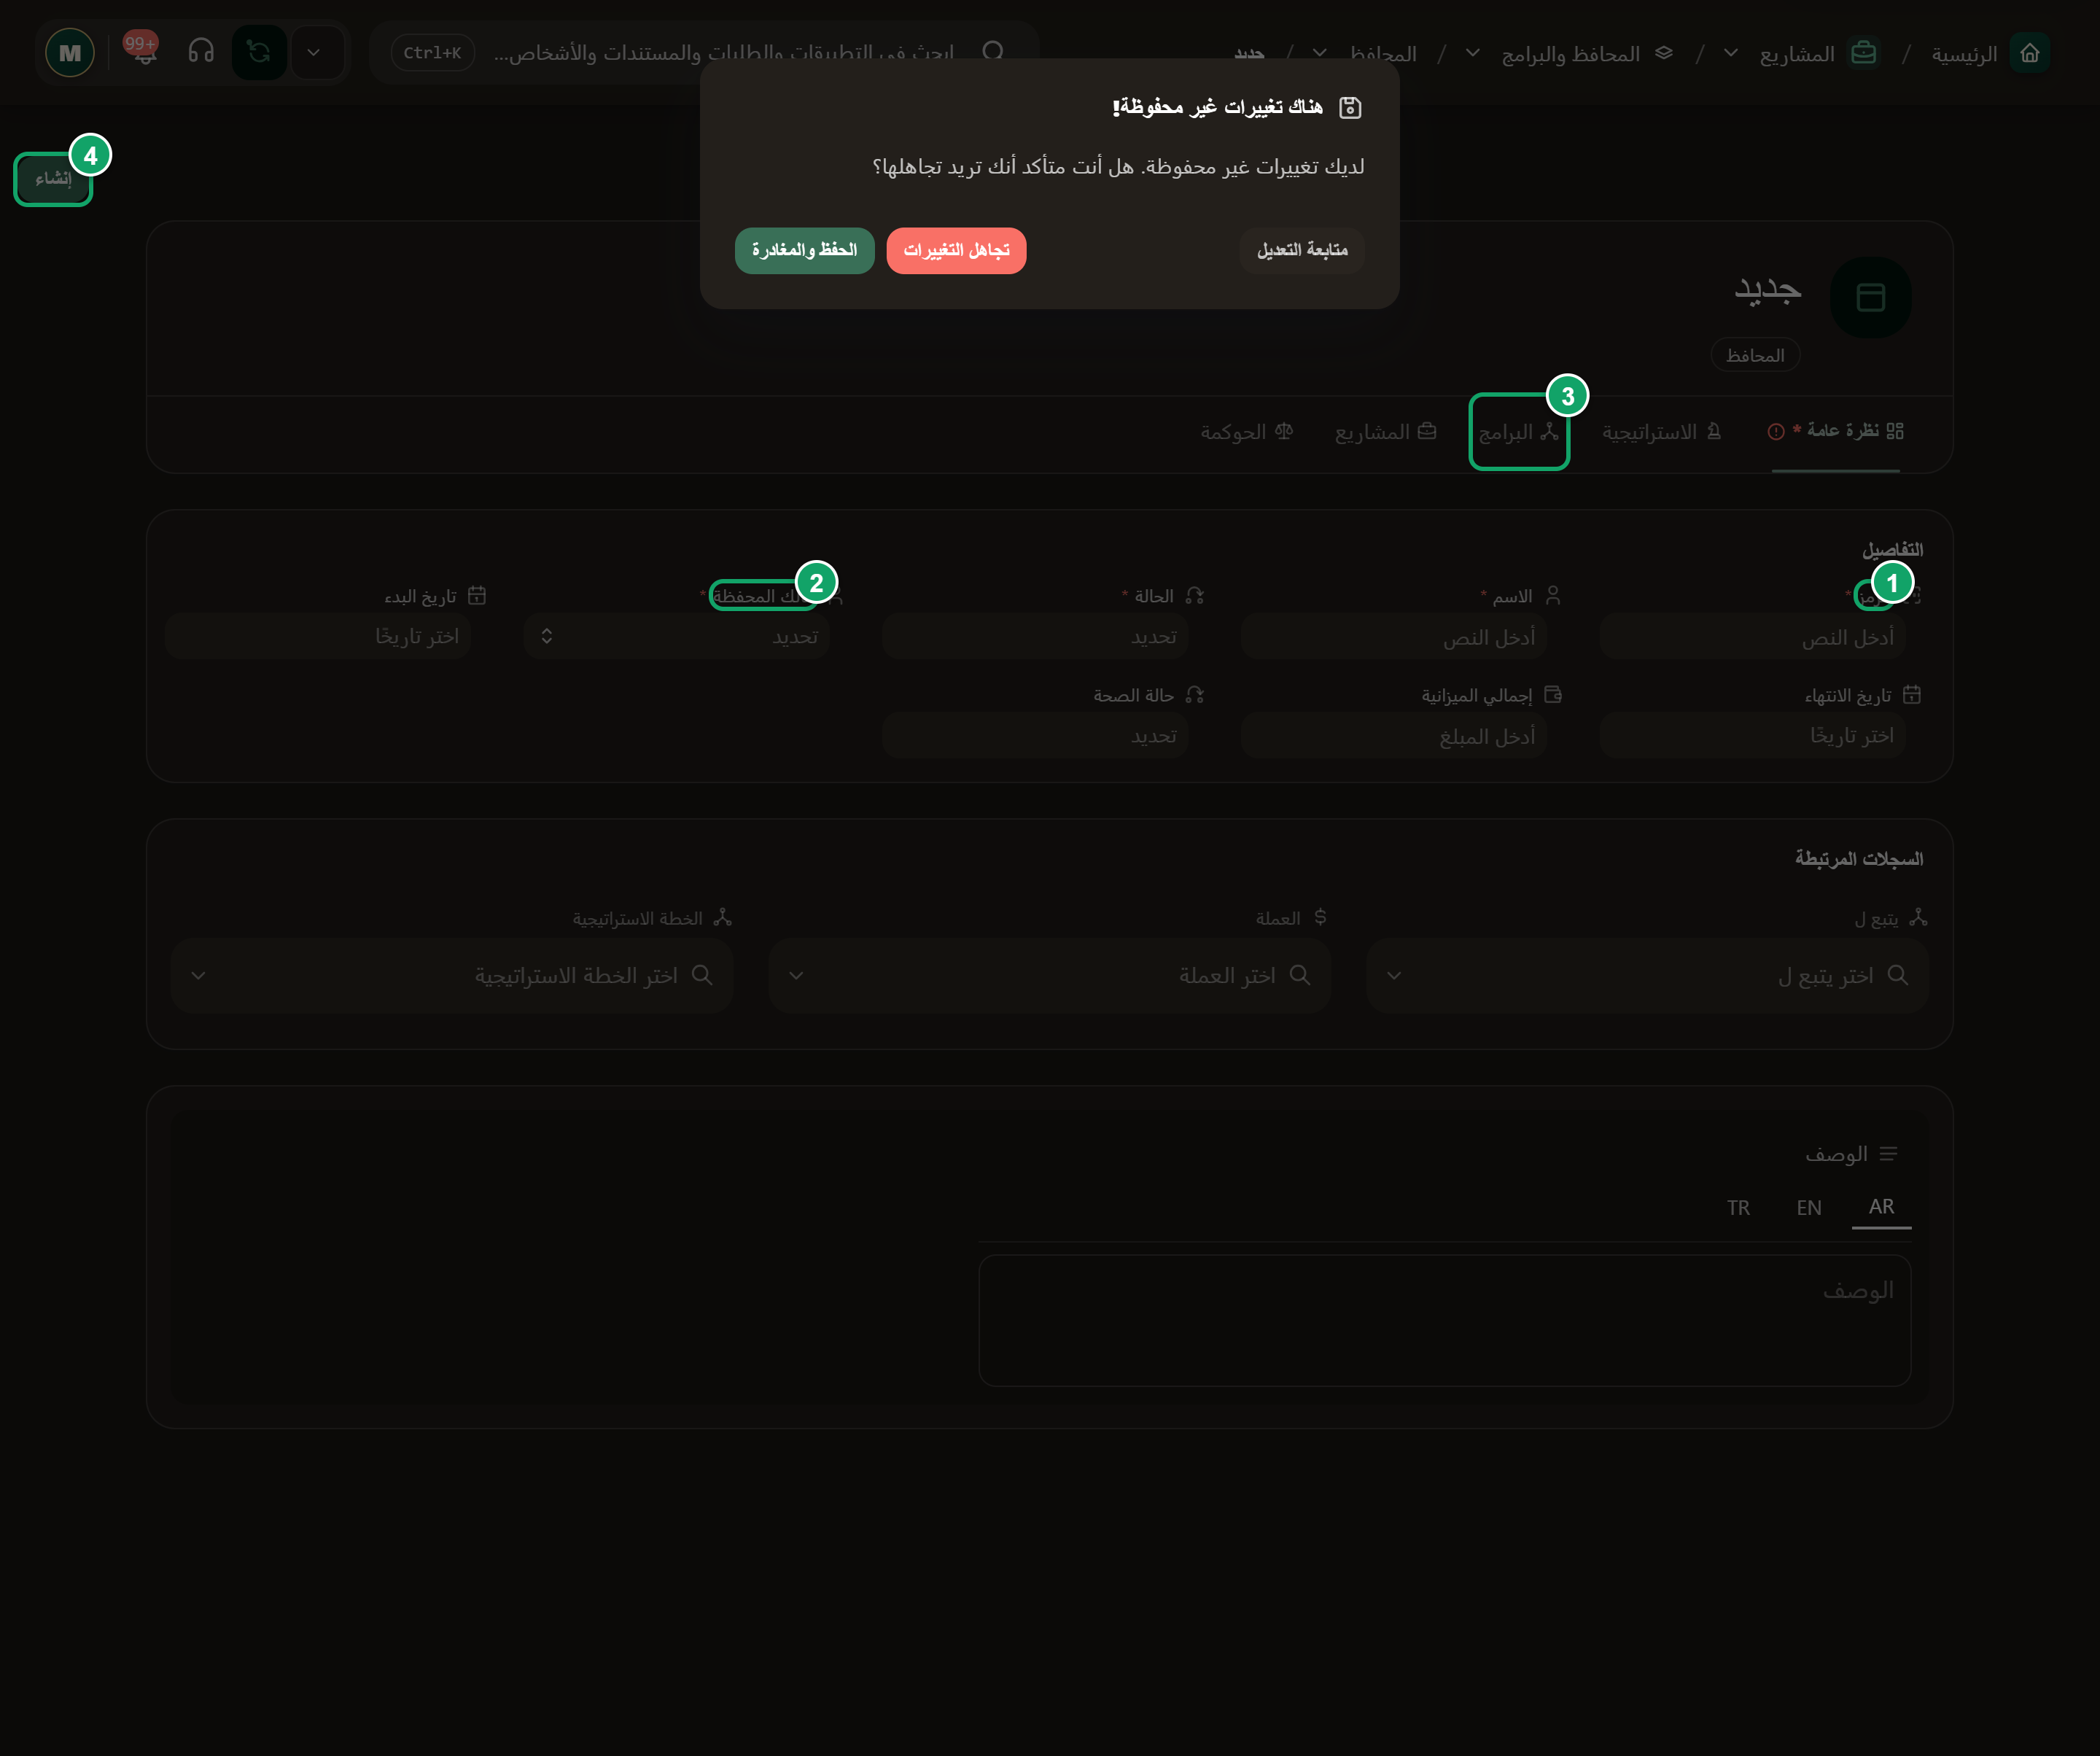
\includegraphics[width=0.95\linewidth,height=0.72\textheight,keepaspectratio]{figures/screens/ch05-portfolios-ar.png}
\caption{نموذج محفظة جديدة قبل الحفظ}
\label{fig:projects-screen-portfolios}
\shotnote{تحدد بيانات المحفظة اسمها ومالكها وحالتها قبل ربط البرامج والمشاريع بها. يظهر الربط بالخطة الاستراتيجية والعملة ضمن البيانات المرتبطة، بينما يبقى إنشاء المحفظة خطوة مستقلة عن إنشاء البرامج التي قد تتبعها. ① «الرمز»: رمز فريد للمحفظة. ② «مالك المحفظة». ③ تبويب «البرامج» الذي يجمع برامج المحفظة. ④ «إنشاء».}
\end{figure}
\begin{table}[H]
\centering
\caption{ما الذي تسجّله؟}
\label{tab:projects-portfolios-fields}
\begin{tabularx}{\linewidth}{R{4.2cm} Y}
\rcHeaderRow
\thh{نوع البيانات} & \thh{الحقول}\\
بيانات إلزامية & «الرمز»، «الاسم»، «الحالة»، «مالك المحفظة».\\
بيانات إضافية & «الوصف»، «التوافق الاستراتيجي»، «تاريخ البدء»، «تاريخ الانتهاء»، «إجمالي الميزانية»، «العملة»، «حالة الصحة»، «طريقة تحديد الأولويات»، «مستوى النضج»، «الخطة الاستراتيجية»، «الوسوم».\\
\end{tabularx}
\end{table}
\begin{table}[H]
\centering
\caption{التبويبات والسجلات المرتبطة}
\label{tab:projects-portfolios-tabs}
\begin{tabularx}{\linewidth}{R{4.2cm} Y}
\rcHeaderRow
\thh{التبويب} & \thh{ما الذي تجده فيه؟}\\
«نظرة عامة» & «ملخص المحفظة»؛ «الجدول الزمني والصحة»\\
«الاستراتيجية» & «المواءمة الاستراتيجية»\\
«البرامج» & البرامج (\ref{sec:projects-feature-programs})\\
«المشاريع» & المشاريع (\ref{sec:projects-feature-projects})\\
«المالية» & يعرض المعلومات المرتبطة بهذا الجانب عندما تنطبق إعدادات السجل.\\
«الحوكمة» & «نموذج الحوكمة»؛ مراجعات التخطيط (\ref{sec:projects-feature-planning-reviews})؛ اعتمادات التخطيط (\ref{sec:projects-feature-planning-approvals})؛ قرارات التخطيط (\ref{sec:projects-feature-planning-decisions})\\
\end{tabularx}
\end{table}
\begin{figure}[H]
\centering
\begin{tikzpicture}[node distance=0.5cm]
\node[stepBox] (n0) {\RL{اختيار صفحة العمل}};
\node[stepBox,below=of n0] (n1) {\RL{المحافظ}};
\node[stepBox,below=of n1] (n2) {\RL{الحفظ ثم إعادة الفتح}};
\draw[flowsTo] (n0) -- (n1);
\draw[flowsTo] (n1) -- (n2);
\end{tikzpicture}
\rclegend
\caption{مسار العمل والتحقق}
\label{fig:projects-portfolios-flow}
\shotnote{يبدأ العمل بفتح «المحافظ» واختيار السجل الصحيح قبل إدخال التفاصيل. إعادة فتحه بعد الحفظ تؤكد بقاء البيانات، لكنها لا تعني اعتمادها أو اكتمال العمل المرتبط بها.}
\end{figure}

\subsection{خطوات العمل والتحقق}
\begin{enumerate}
\item افتح «المحافظ» واضغط «إضافة». أدخل الرمز والاسم واختر الحالة ومالك المحفظة.
\item أكمل معلومات التوجه والتواريخ والميزانية عندما تحتاج إليها، ثم اضغط «إنشاء». لا تعتبر مبلغ الميزانية وحده دليلاً على وجود تمويل متاح.
\item أعد فتح المحفظة وراجع مالكها وحالتها. عند ربط برنامج أو مشروع، اختر هذه المحفظة في السجل المعني ثم تحقق من ظهوره ضمن سجلاتها المرتبطة.
\end{enumerate}

\textbf{تطبيق المثال:} في المثال الافتراضي، استخدم «تطوير فروع الأفق» في «الاسم»، ثم أكمل بقية البيانات بما يناسب عمل الأفق. لا تستخدم قيم المثال بديلاً عن السجلات الفعلية المطلوبة في حقول الربط.

\textbf{تحقق ومعالجة المشكلة:} يجب أن تجد السجل بعد إعادة فتحه وأن تبقى البيانات التي حفظتها. إذا لم يظهر، فراجع البحث والفلاتر والنطاق وصلاحية الوصول قبل إنشائه مرة أخرى. وإذا تعذر الحفظ، فأكمل الحقول المطلوبة ورسائل التحقق؛ أما غياب تبويب أو قفل حقل فيستدعي مراجعة نوع السجل وإطاره ومرحلته مع المسؤول.

\clearpage
\section{البرامج}
\label{sec:projects-feature-programs}

ينسّق البرنامج مشاريع مترابطة لتحقيق فائدة مشتركة. يراجع مدير البرنامج المشاريع والنتائج والموارد معاً، ويمكن ربط البرنامج بمحفظة عند الحاجة.

\begin{rcnote}[مثال: شركة الأفق]
تربط سارة مشروع زيارة حلب ببرنامج «تحسين خدمات الفروع» بعد الاتفاق مع مديره. يظهر المشروع ضمن أعمال البرنامج، فتُراجع فائدته مع بقية المشاريع المرتبطة.
\end{rcnote}

\textbf{المسار ومن يستخدمه:} افتح تطبيق «المشاريع»، ثم بطاقة «البرامج». هذه صفحة رئيسية في التطبيق. يستخدمها المسؤول عن هذا العمل، ويعدّل الموظف البيانات المسموح له بها وفق صلاحياته.

\begin{figure}[H]
\centering
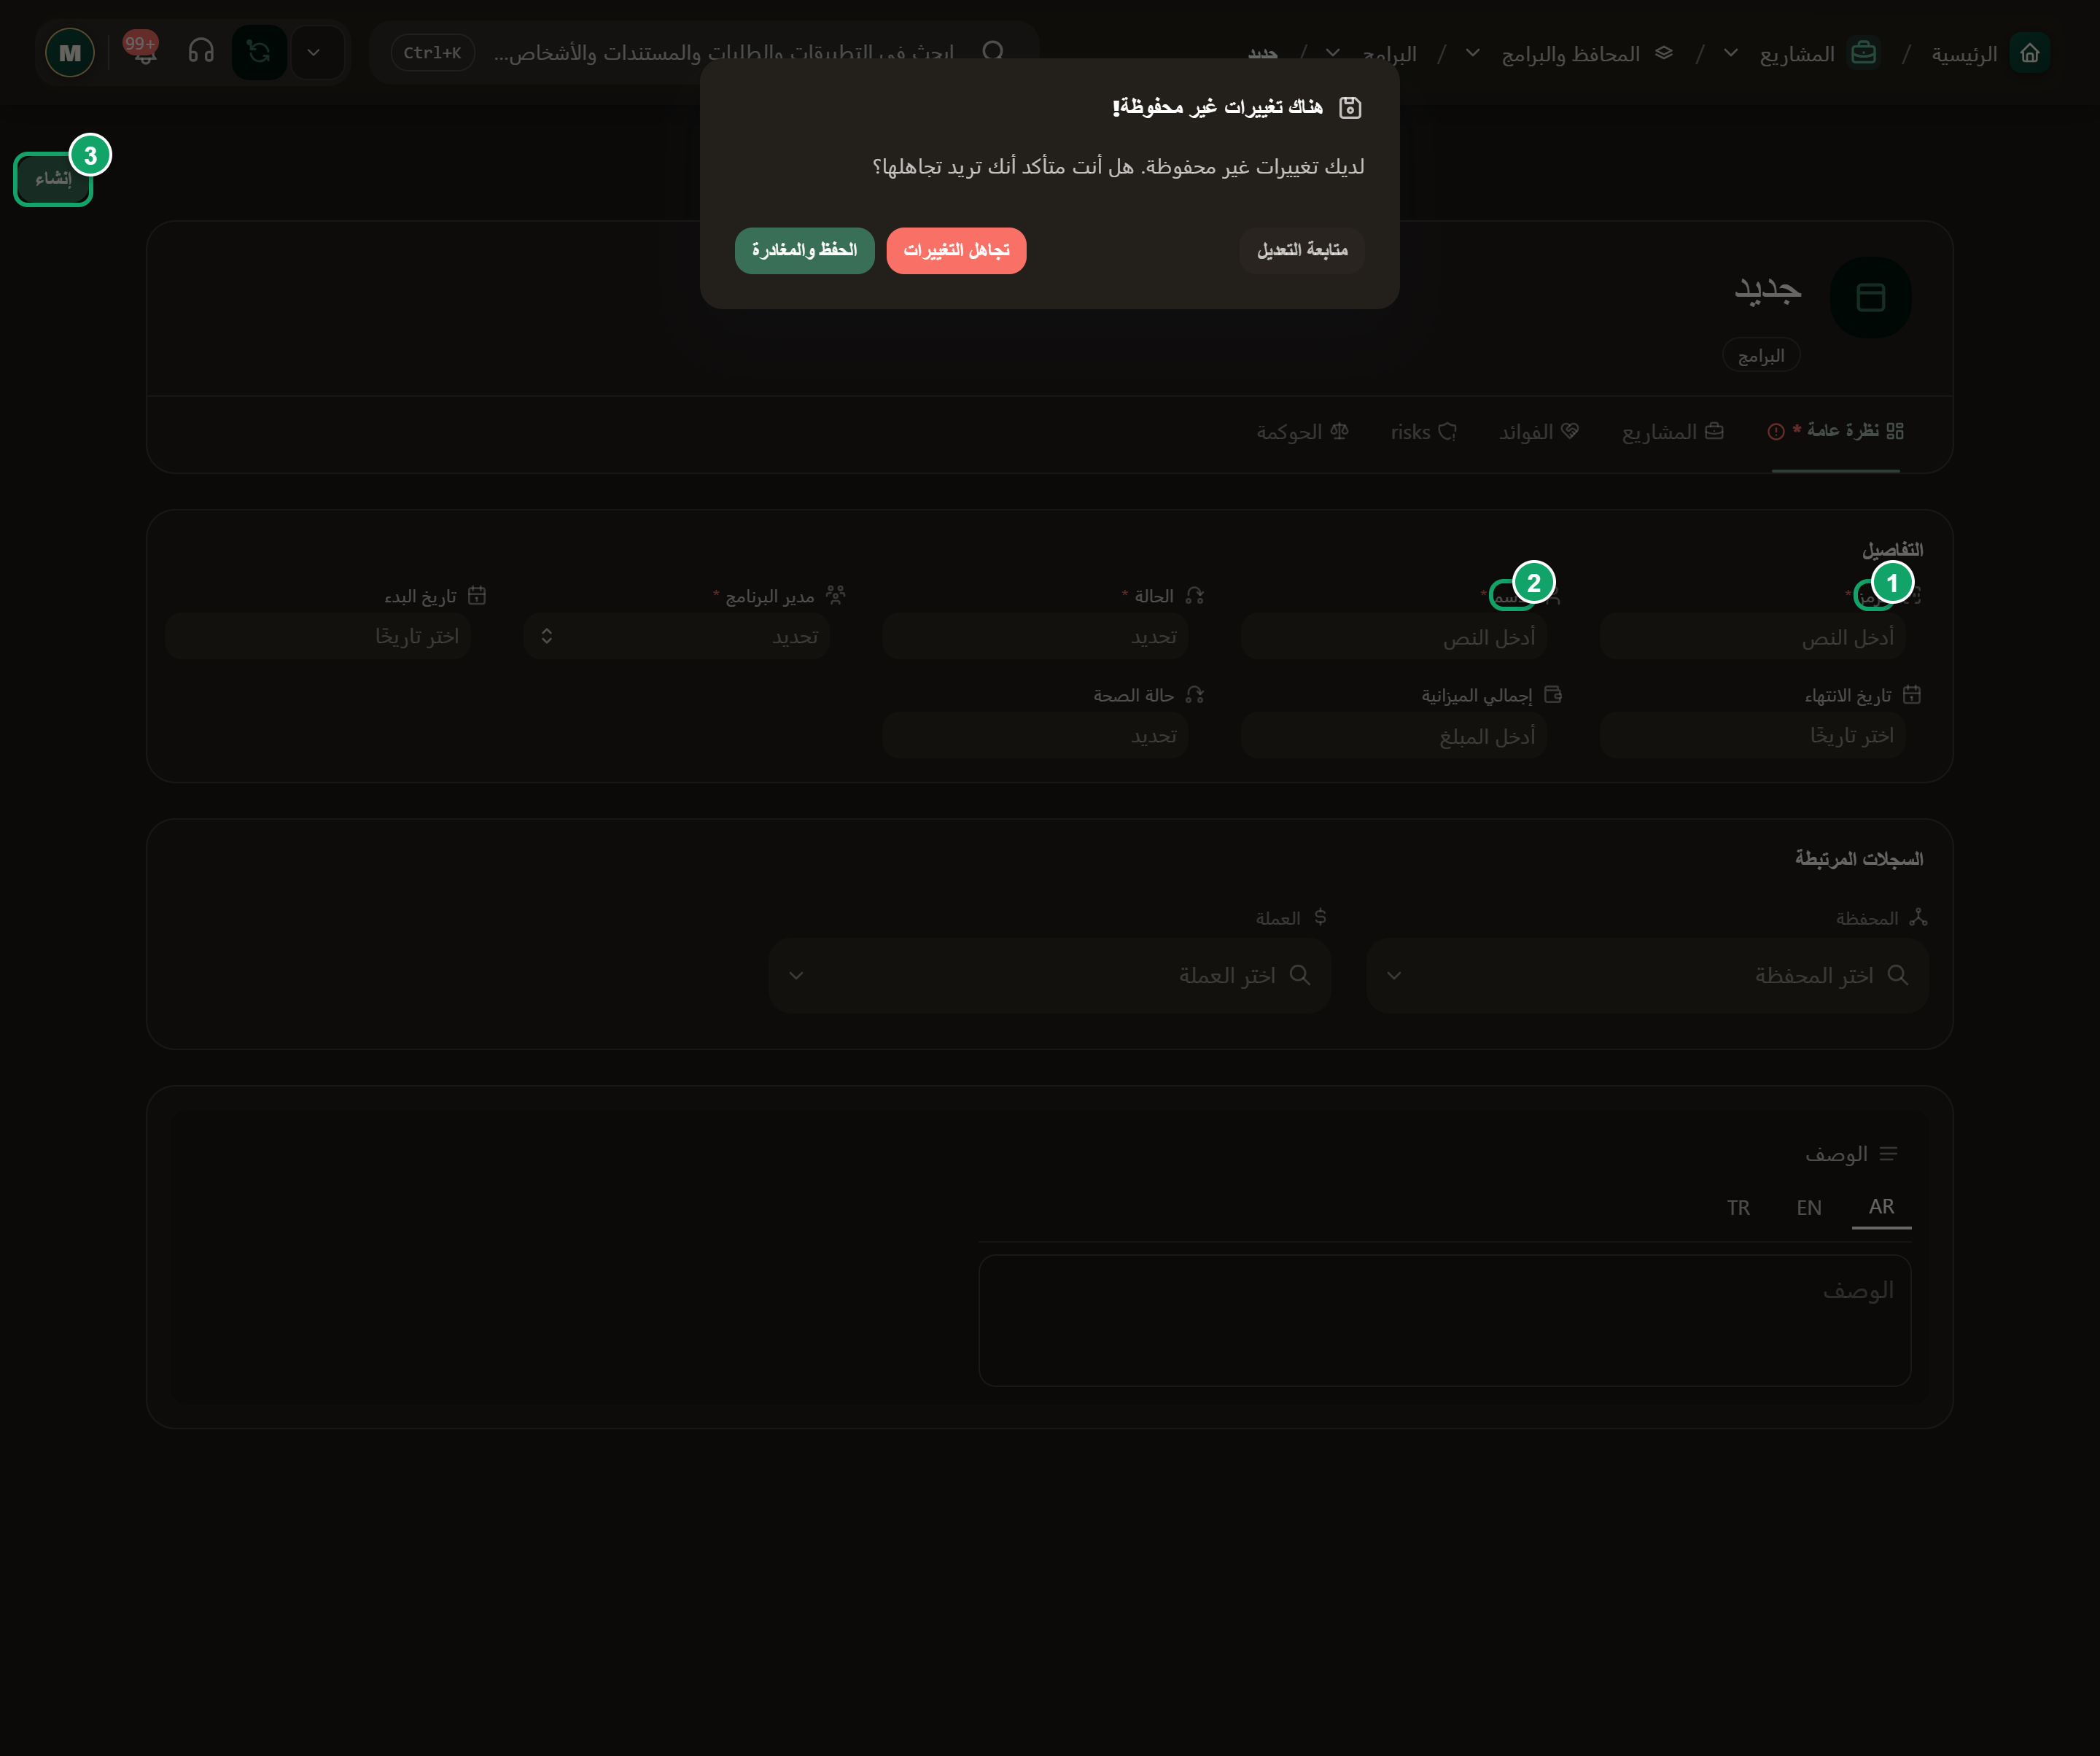
\includegraphics[width=0.95\linewidth,height=0.72\textheight,keepaspectratio]{figures/screens/ch05-programs-ar.png}
\caption{نموذج برنامج جديد قبل الحفظ}
\label{fig:projects-screen-programs}
\shotnote{يعرض النموذج مدير البرنامج وحالته والتواريخ، مع ربط اختياري بالمحفظة. تساعد هذه البيانات على تحديد من ينسّق المشاريع المرتبطة، ولا يعني اختيار محفظة أن المشاريع أُضيفت إلى البرنامج تلقائياً. ① «الرمز» و② «الاسم»: أول حقلين يعرّفان البرنامج. ③ «إنشاء».}
\end{figure}
\begin{table}[H]
\centering
\caption{ما الذي تسجّله؟}
\label{tab:projects-programs-fields}
\begin{tabularx}{\linewidth}{R{4.2cm} Y}
\rcHeaderRow
\thh{نوع البيانات} & \thh{الحقول}\\
بيانات إلزامية & «الرمز»، «الاسم»، «الحالة»، «مدير البرنامج».\\
بيانات إضافية & «الوصف»، «المحفظة»، «الراعي»، «تاريخ البدء»، «تاريخ الانتهاء»، «إجمالي الميزانية»، «العملة»، «حالة الصحة»، «ملخص الفوائد»، «الخطة الاستراتيجية»، «الوسوم».\\
\end{tabularx}
\end{table}
\begin{table}[H]
\centering
\caption{التبويبات والسجلات المرتبطة}
\label{tab:projects-programs-tabs}
\begin{tabularx}{\linewidth}{R{4.2cm} Y}
\rcHeaderRow
\thh{التبويب} & \thh{ما الذي تجده فيه؟}\\
«نظرة عامة» & «ملخص البرنامج»\\
«المشاريع» & المشاريع (\ref{sec:projects-feature-projects})\\
«الفوائد» & «حالة الفوائد»\\
«المالية» & يعرض المعلومات المرتبطة بهذا الجانب عندما تنطبق إعدادات السجل.\\
«التنفيذ» & «سياق التنفيذ»\\
«الحوكمة» & «الحوكمة»؛ مراجعات التخطيط (\ref{sec:projects-feature-planning-reviews})؛ اعتمادات التخطيط (\ref{sec:projects-feature-planning-approvals})؛ قرارات التخطيط (\ref{sec:projects-feature-planning-decisions})\\
\end{tabularx}
\end{table}
\begin{figure}[H]
\centering
\begin{tikzpicture}[node distance=0.5cm]
\node[stepBox] (n0) {\RL{اختيار صفحة العمل}};
\node[stepBox,below=of n0] (n1) {\RL{البرامج}};
\node[stepBox,below=of n1] (n2) {\RL{الحفظ ثم إعادة الفتح}};
\draw[flowsTo] (n0) -- (n1);
\draw[flowsTo] (n1) -- (n2);
\end{tikzpicture}
\rclegend
\caption{مسار العمل والتحقق}
\label{fig:projects-programs-flow}
\shotnote{يبدأ العمل بفتح «البرامج» واختيار السجل الصحيح قبل إدخال التفاصيل. إعادة فتحه بعد الحفظ تؤكد بقاء البيانات، لكنها لا تعني اعتمادها أو اكتمال العمل المرتبط بها.}
\end{figure}

\subsection{خطوات العمل والتحقق}
\begin{enumerate}
\item افتح «البرامج» واضغط «إضافة». أدخل الرمز والاسم واختر الحالة ومدير البرنامج.
\item اختر المحفظة إذا كان البرنامج يتبعها، ثم اكتب الفوائد المتوقعة والتواريخ والمعلومات المالية المتاحة. اضغط «إنشاء».
\item أعد فتح البرنامج وراجع مديره والفوائد التي يتابعها. اربط المشاريع المناسبة من حقل البرنامج في كل مشروع، وتحقق من قائمة المشاريع المرتبطة.
\end{enumerate}

\textbf{تطبيق المثال:} في المثال الافتراضي، استخدم «تحسين خدمات الفروع» في «الاسم»، ثم أكمل بقية البيانات بما يناسب عمل الأفق. لا تستخدم قيم المثال بديلاً عن السجلات الفعلية المطلوبة في حقول الربط.

\textbf{تحقق ومعالجة المشكلة:} يجب أن تجد السجل بعد إعادة فتحه وأن تبقى البيانات التي حفظتها. إذا لم يظهر، فراجع البحث والفلاتر والنطاق وصلاحية الوصول قبل إنشائه مرة أخرى. وإذا تعذر الحفظ، فأكمل الحقول المطلوبة ورسائل التحقق؛ أما غياب تبويب أو قفل حقل فيستدعي مراجعة نوع السجل وإطاره ومرحلته مع المسؤول.

\clearpage
\section{الميزانيات}
\label{sec:projects-feature-budgets}

تجمع الميزانية بنود التكلفة ومصادر التمويل والمصروفات في سجل واحد. يراجع المسؤول المالي المبلغ المخطط وما سُجّل فعلياً قبل اتخاذ قرار بشأن الإنفاق.

\begin{rcnote}[مثال: شركة الأفق]
تنسّق سارة مع المسؤول المالي لإعداد ميزانية زيارة حلب. يسجّل المسؤول بند الانتقال ثم يقارن المبلغ المخطط بالمصروفات المسجّلة للعملة والفترة نفسيهما.
\end{rcnote}

\textbf{المسار ومن يستخدمه:} افتح تطبيق «المشاريع»، ثم بطاقة «الميزانيات». هذه صفحة رئيسية في التطبيق. يستخدمها المسؤول عن هذا العمل، ويعدّل الموظف البيانات المسموح له بها وفق صلاحياته.

\begin{figure}[H]
\centering
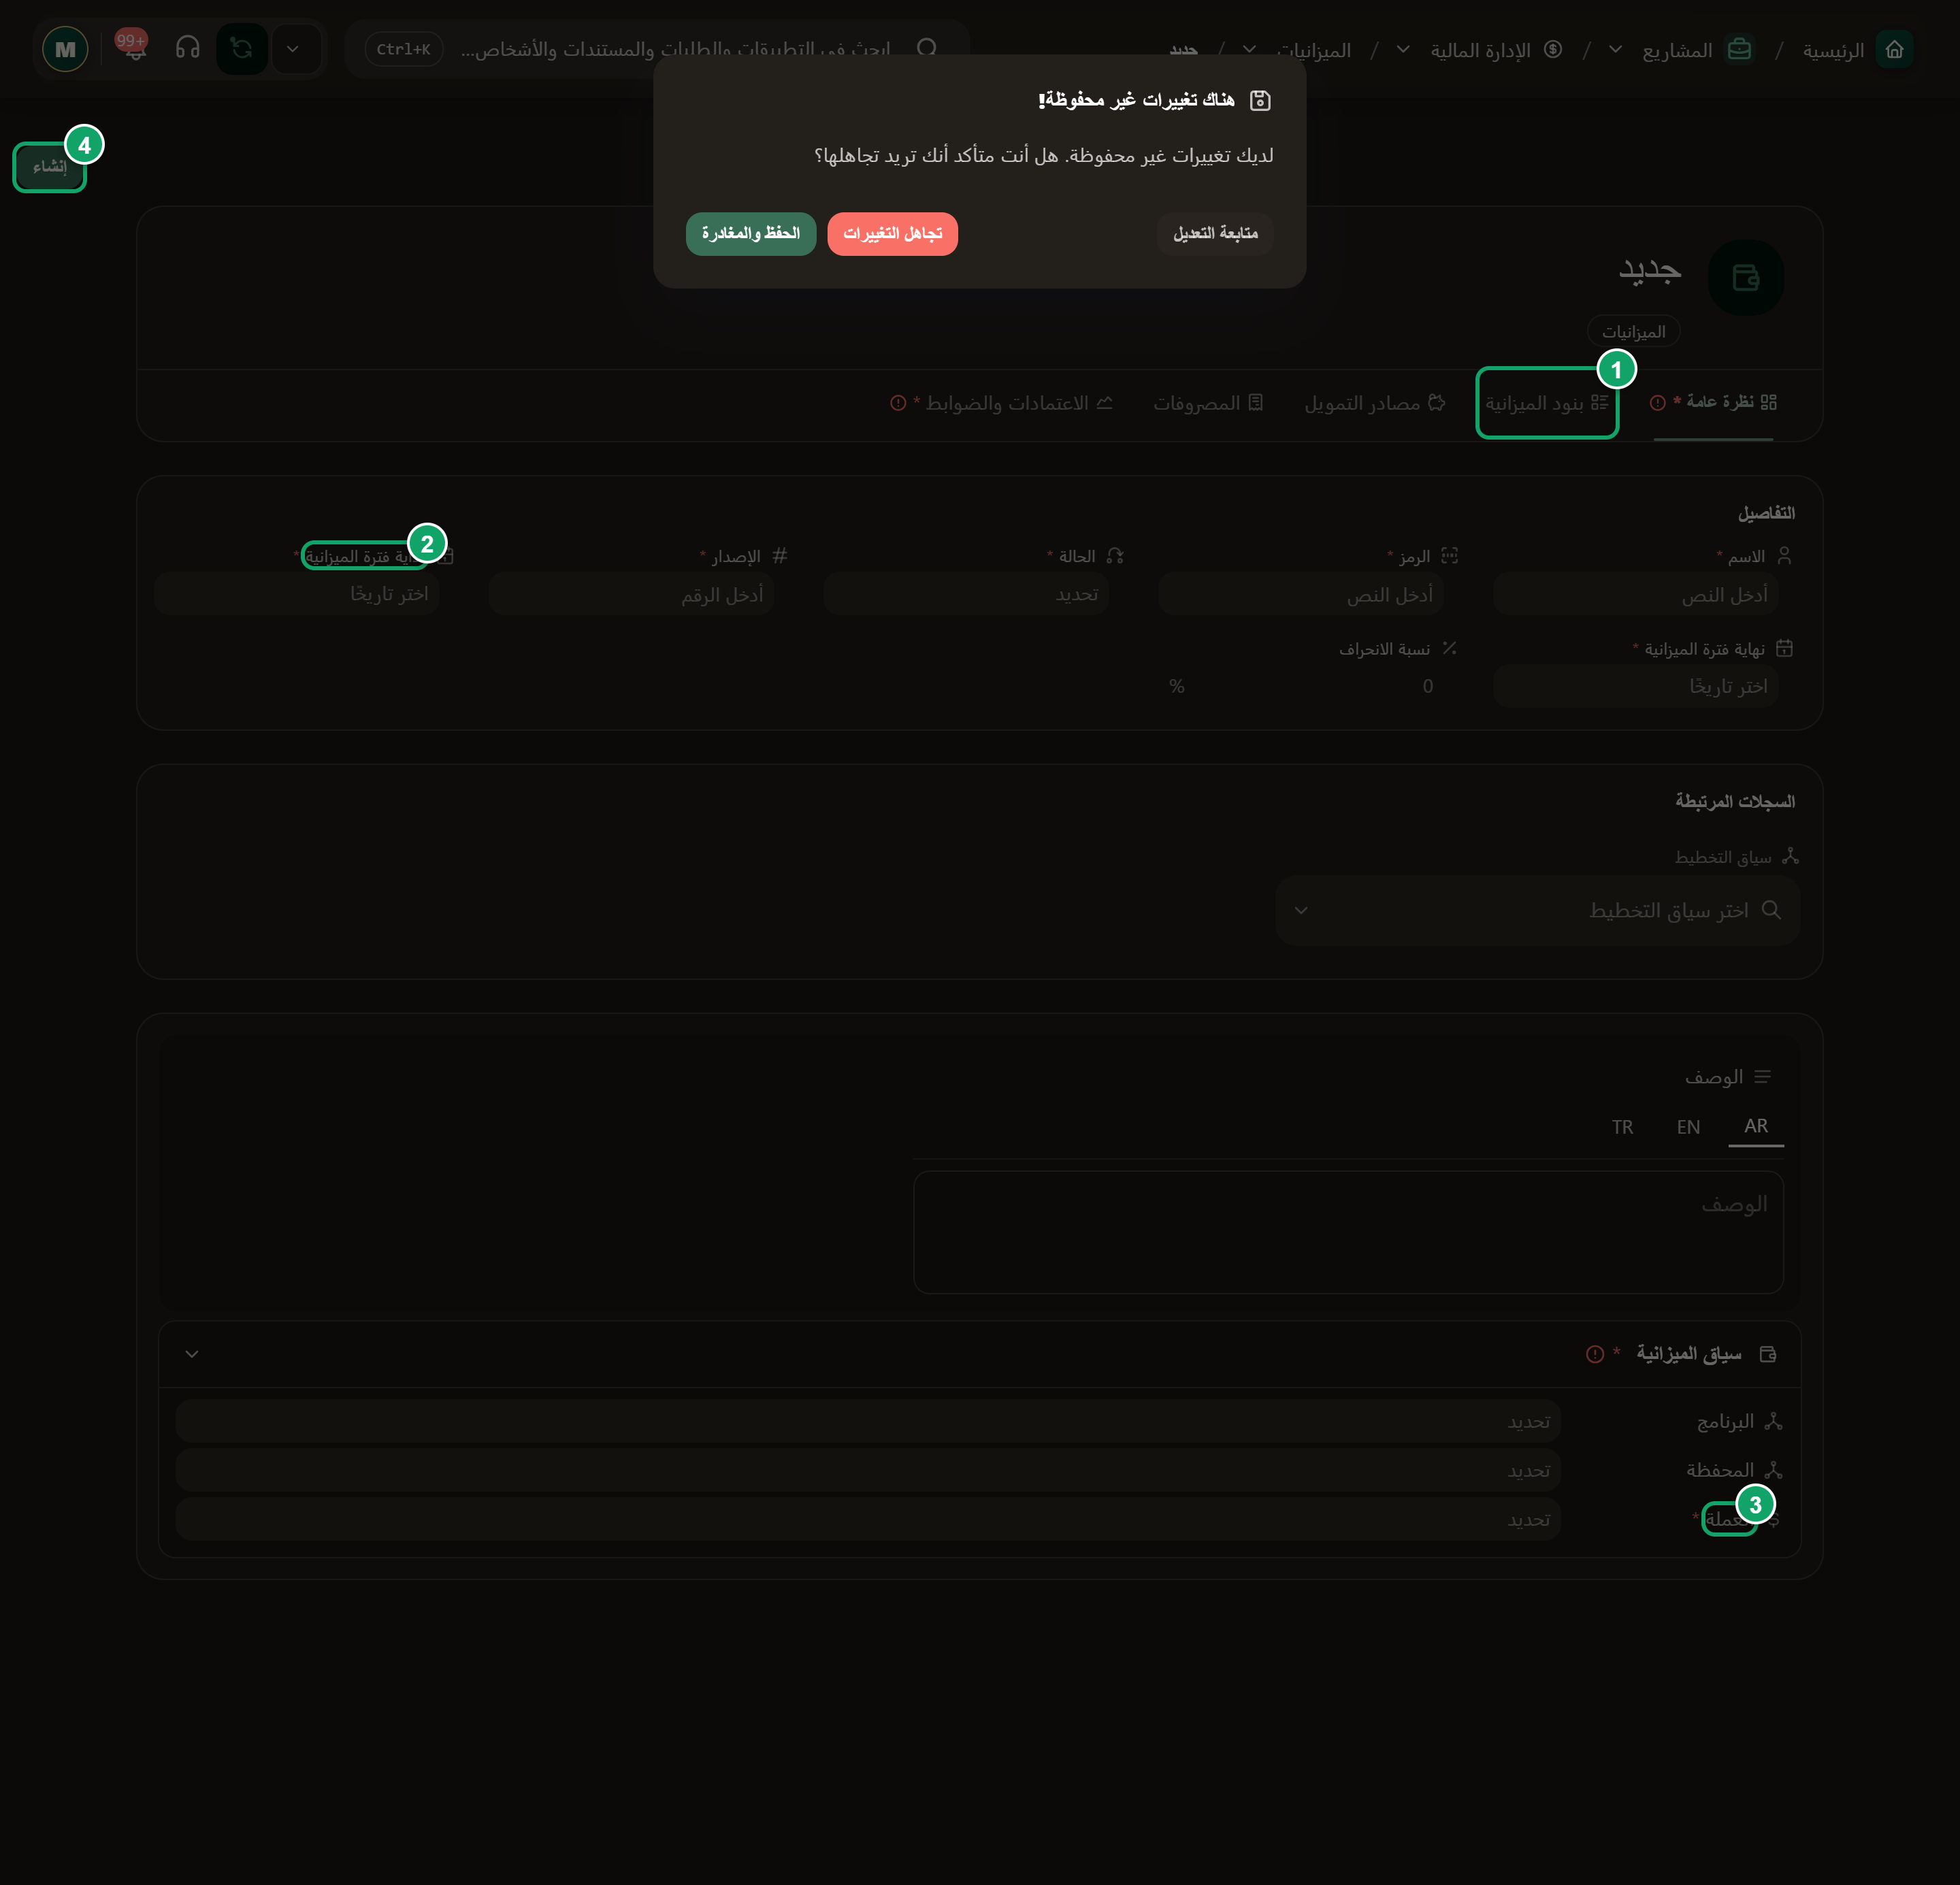
\includegraphics[width=0.95\linewidth,height=0.72\textheight,keepaspectratio]{figures/screens/ch05-budgets-ar.png}
\caption{إعداد ميزانية جديدة قبل الحفظ}
\label{fig:projects-screen-budgets}
\shotnote{يربط النموذج اسم الميزانية وإصدارها بفترة وعملة محددتين، ويتيح اختيار سياق العمل. أما البنود والتمويل والمصروفات فلها أقسامها؛ لذلك لا تمثّل هذه الشاشة وحدها ميزانية مكتملة أو عملية إنفاق. ① تبويب «بنود الميزانية» الذي تُفصَّل فيه المبالغ. ② «بداية فترة الميزانية». ③ «العملة» في سياق الميزانية. ④ «إنشاء».}
\end{figure}
\begin{table}[H]
\centering
\caption{ما الذي تسجّله؟}
\label{tab:projects-budgets-fields}
\begin{tabularx}{\linewidth}{R{4.2cm} Y}
\rcHeaderRow
\thh{نوع البيانات} & \thh{الحقول}\\
بيانات إلزامية & «الاسم»، «الرمز»، «الحالة»، «الإصدار»، «الإصدار الحالي»، «العملة»، «بداية فترة الميزانية»، «نهاية فترة الميزانية»، «أعد بواسطة».\\
بيانات إضافية & «الوصف»، «سياق التخطيط»، «البرنامج»، «المحفظة»، «الإصدار السابق»، «إجمالي المخطط»، «إجمالي الفعلي»، «إجمالي الملتزم»، «إجمالي المتاح»، «إجمالي الممول»، «فجوة التمويل»، «نسبة الانحراف»، «مبلغ الطوارئ»، «نسبة الطوارئ»، «اعتمد بواسطة»، «تاريخ الاعتماد»، «ملاحظات».\\
\end{tabularx}
\end{table}
\begin{table}[H]
\centering
\caption{التبويبات والسجلات المرتبطة}
\label{tab:projects-budgets-tabs}
\begin{tabularx}{\linewidth}{R{4.2cm} Y}
\rcHeaderRow
\thh{التبويب} & \thh{ما الذي تجده فيه؟}\\
«نظرة عامة» & «سياق الميزانية»؛ «إجماليات الميزانية»\\
«بنود الميزانية» & بنود الميزانية (\ref{sec:projects-feature-budget-lines})\\
«مصادر التمويل» & «حالة التمويل»؛ مصادر التمويل (\ref{sec:projects-feature-funding-sources})\\
«المصروفات» & المصروفات (\ref{sec:projects-feature-expenditures})\\
«الاعتمادات والضوابط» & «الإصدارات»؛ «الاعتمادات»؛ «ضوابط التوقع»\\
\end{tabularx}
\end{table}
\begin{figure}[H]
\centering
\begin{tikzpicture}[node distance=0.5cm]
\node[stepBox] (n0) {\RL{اختيار صفحة العمل}};
\node[stepBox,below=of n0] (n1) {\RL{الميزانيات}};
\node[stepBox,below=of n1] (n2) {\RL{الحفظ ثم إعادة الفتح}};
\draw[flowsTo] (n0) -- (n1);
\draw[flowsTo] (n1) -- (n2);
\end{tikzpicture}
\rclegend
\caption{مسار العمل والتحقق}
\label{fig:projects-budgets-flow}
\shotnote{يبدأ العمل بفتح «الميزانيات» واختيار السجل الصحيح قبل إدخال التفاصيل. إعادة فتحه بعد الحفظ تؤكد بقاء البيانات، لكنها لا تعني اعتمادها أو اكتمال العمل المرتبط بها.}
\end{figure}

\subsection{خطوات العمل والتحقق}
\begin{enumerate}
\item افتح «الميزانيات» في تطبيق «المشاريع» واضغط «إضافة». أدخل الرمز والاسم واختر العملة وبداية فترة الميزانية ونهايتها.
\item راجع الحالة والإصدار و«الإصدار الحالي» و«أعد بواسطة». اربط الميزانية بسياق العمل المقصود عند الحاجة، ثم اضغط «إنشاء».
\item أعد فتح الميزانية وأضف بنودها من «بنود الميزانية». راجع نوع كل بند وطريقة احتسابه قبل تفسير الإجمالي.
\item تابع مصادر التمويل والمصروفات في أقسامها. تحقق من الإصدار والعملة والفترة عند المقارنة، ولا تخلط التعهد بالتمويل بالمبلغ المستلم أو المصروف المدفوع.
\end{enumerate}

\textbf{تطبيق المثال:} في المثال الافتراضي، استخدم «ميزانية زيارة فرع حلب» في «الاسم»، ثم أكمل بقية البيانات بما يناسب عمل الأفق. لا تستخدم قيم المثال بديلاً عن السجلات الفعلية المطلوبة في حقول الربط.

\textbf{تحقق ومعالجة المشكلة:} يجب أن تجد السجل بعد إعادة فتحه وأن تبقى البيانات التي حفظتها. إذا لم يظهر، فراجع البحث والفلاتر والنطاق وصلاحية الوصول قبل إنشائه مرة أخرى. وإذا تعذر الحفظ، فأكمل الحقول المطلوبة ورسائل التحقق؛ أما غياب تبويب أو قفل حقل فيستدعي مراجعة نوع السجل وإطاره ومرحلته مع المسؤول.

\clearpage
\section{فئات التكلفة}
\label{sec:projects-feature-cost-categories}

توحّد فئات التكلفة طريقة تصنيف بنود الميزانية، مثل السفر والتجهيزات. يهيّئها المسؤول المالي كي يمكن مقارنة بنود متشابهة بدلاً من توزيعها على تسميات مختلفة.

\begin{rcnote}[مثال: شركة الأفق]
يهيّئ المسؤول المالي فئة «السفر والانتقال» بالرمز \en{HZN-C-01} والنوع «سفر». تستخدم سارة هذه الفئة عند تصنيف بند انتقال فريق الزيارة، فتظل تكاليف السفر مجمّعة تحت تسمية واحدة.
\end{rcnote}

\textbf{المسار ومن يستخدمه:} افتح تطبيق «المشاريع»، ثم بطاقة «فئات التكلفة». هذه صفحة رئيسية في التطبيق. يستخدمها المسؤول عن هذا العمل، ويعدّل الموظف البيانات المسموح له بها وفق صلاحياته.

\begin{figure}[H]
\centering
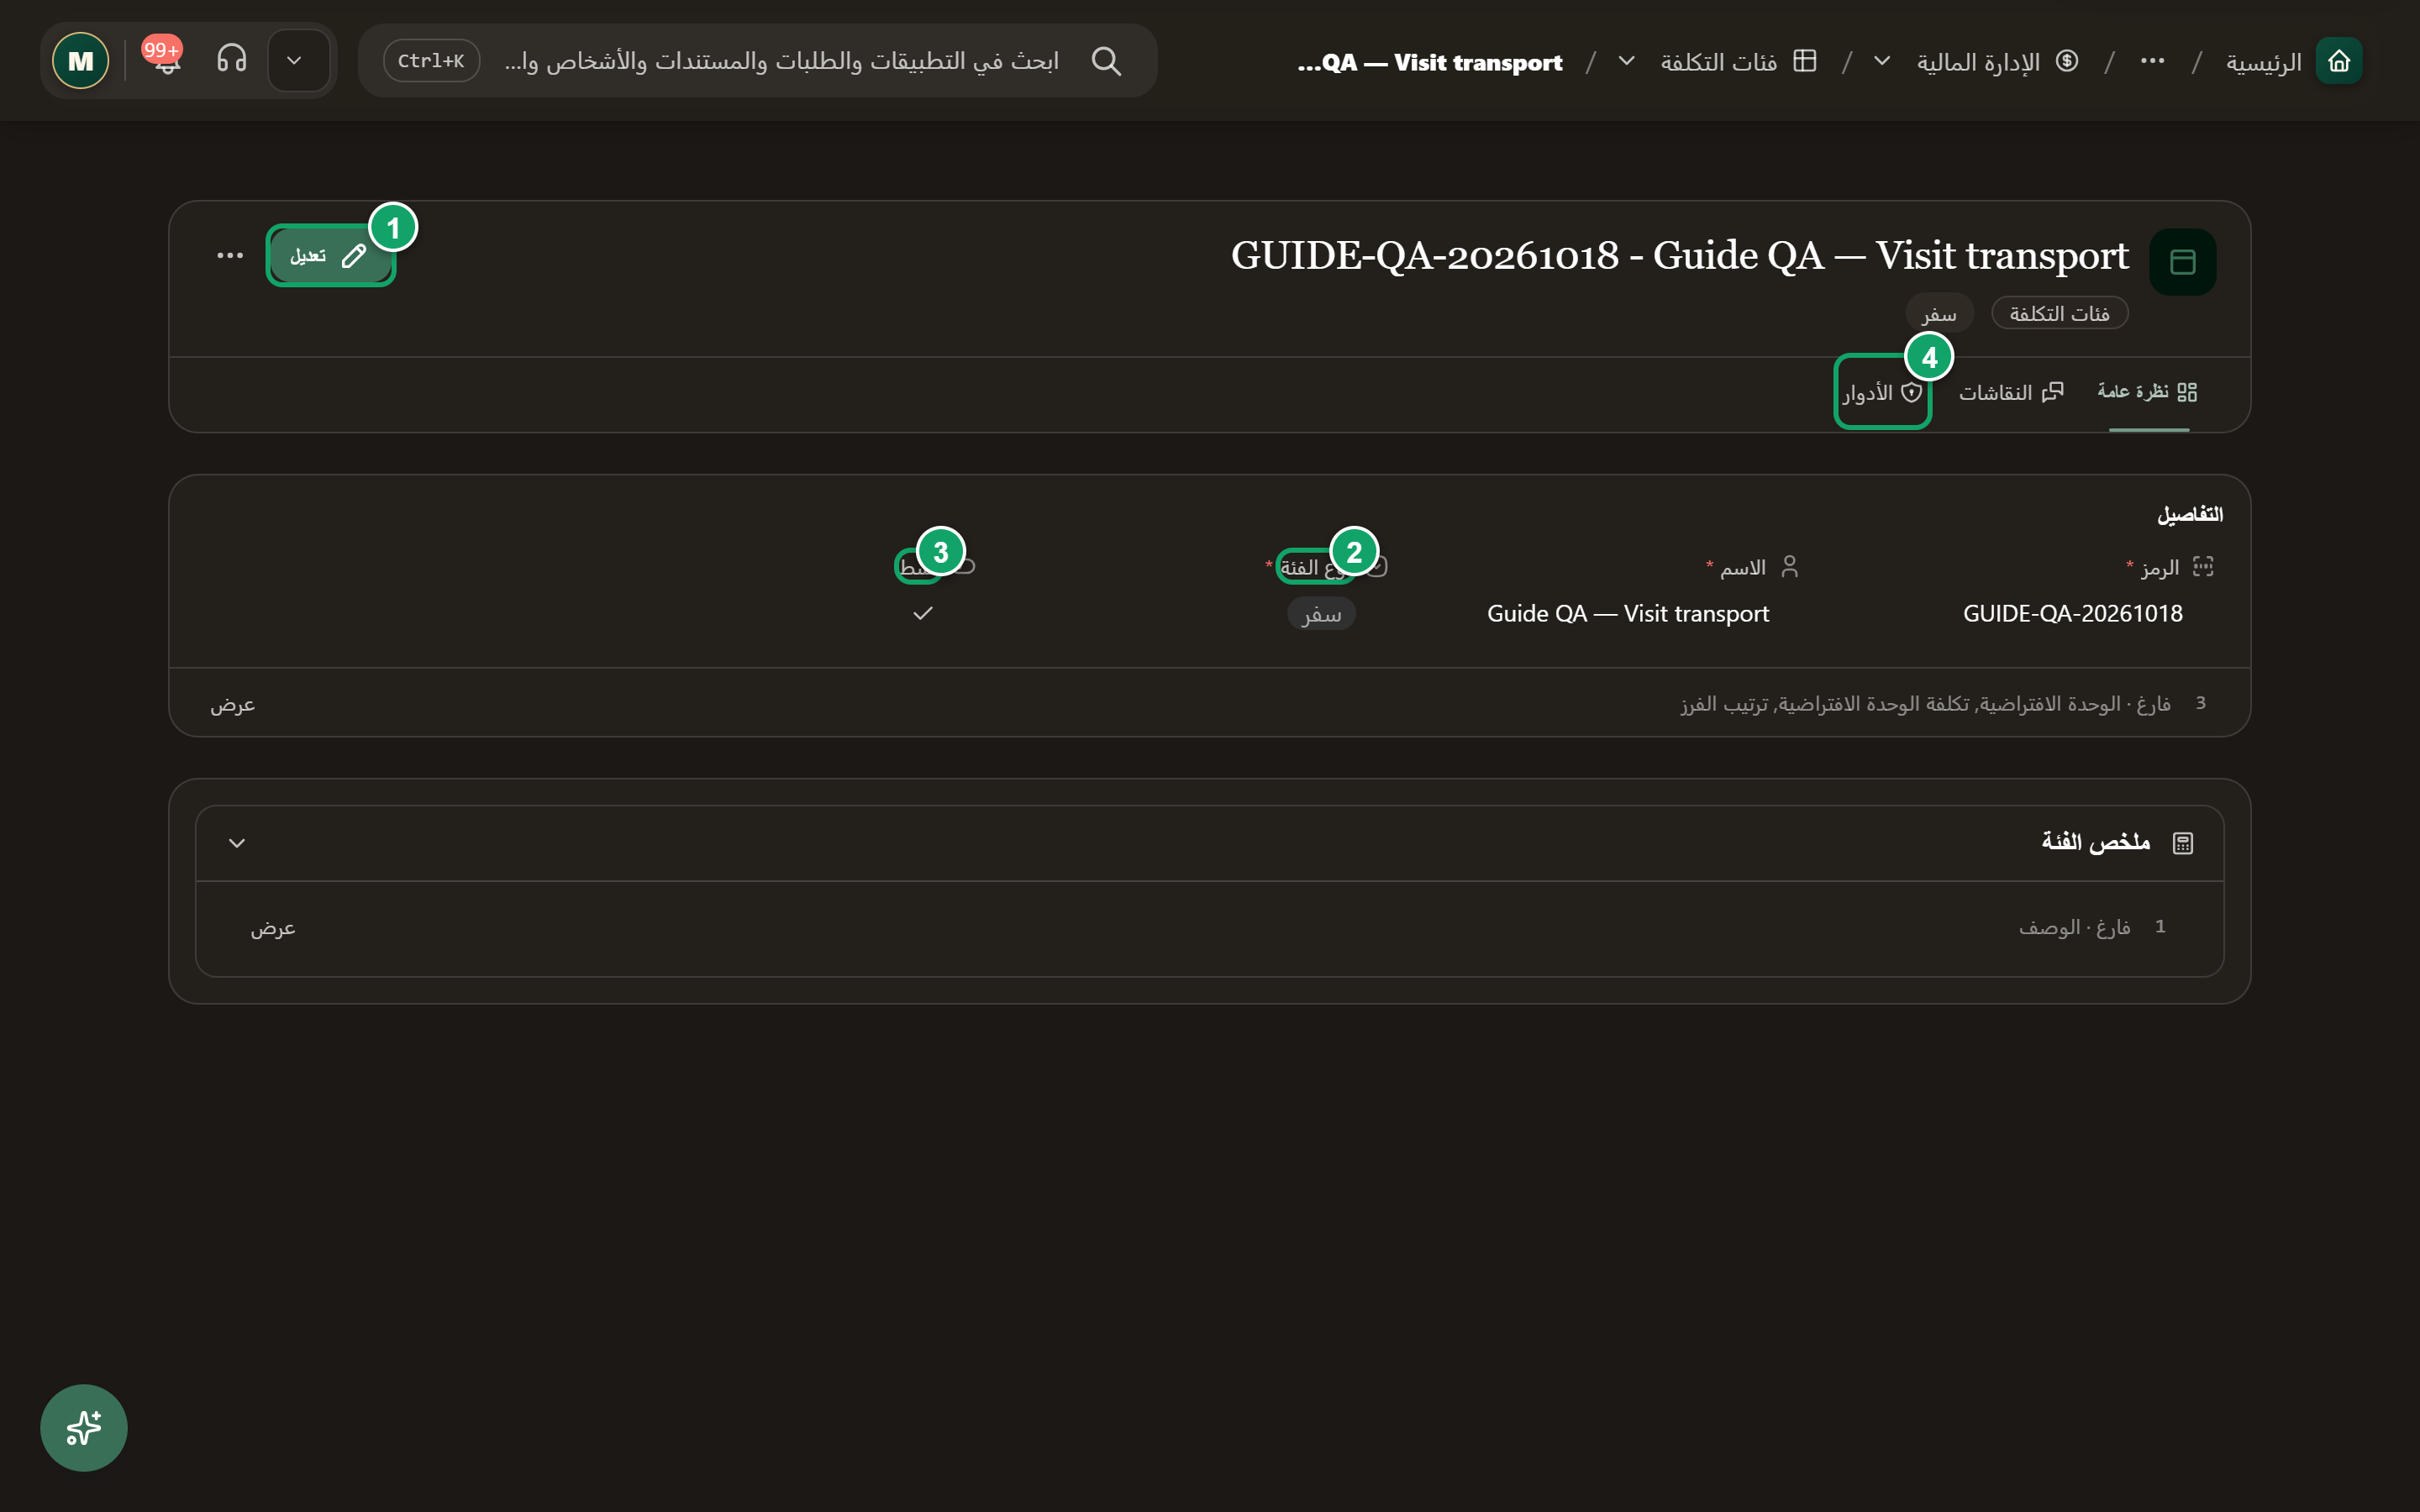
\includegraphics[width=0.95\linewidth,height=0.72\textheight,keepaspectratio]{figures/screens/ch05-cost-category-ar.png}
\caption{فئة تكلفة تجريبية بعد حفظها}
\label{fig:projects-screen-cost-category}
\shotnote{يعرض السجل المحفوظ الرمز والاسم والنوع «سفر»، مع تفعيل الفئة. الحقول الفارغة مخفية ويمكن إظهارها، لذا لا يعني غياب قيمة الوحدة أو تكلفتها أن الحفظ فشل؛ هذا سجل اختبار منفصل عن مثال شركة الأفق. ① «تعديل». ② «نوع الفئة»: يصنّف التكلفة، وهو هنا «سفر». ③ «نشط»: يبيّن أن الفئة متاحة للاستخدام. ④ تبويب «الأدوار» لمن يستطيع رؤية الفئة أو تعديلها.}
\end{figure}
\begin{table}[H]
\centering
\caption{ما الذي تسجّله؟}
\label{tab:projects-cost-categories-fields}
\begin{tabularx}{\linewidth}{R{4.2cm} Y}
\rcHeaderRow
\thh{نوع البيانات} & \thh{الحقول}\\
بيانات إلزامية & «الرمز»، «الاسم»، «نوع الفئة».\\
بيانات إضافية & «الوصف»، «نشط»، «الوحدة الافتراضية»، «تكلفة الوحدة الافتراضية»، «ترتيب الفرز».\\
\end{tabularx}
\end{table}
\begin{table}[H]
\centering
\caption{التبويبات والسجلات المرتبطة}
\label{tab:projects-cost-categories-tabs}
\begin{tabularx}{\linewidth}{R{4.2cm} Y}
\rcHeaderRow
\thh{التبويب} & \thh{ما الذي تجده فيه؟}\\
«نظرة عامة» & «ملخص الفئة»\\
\end{tabularx}
\end{table}
\begin{figure}[H]
\centering
\begin{tikzpicture}[node distance=0.5cm]
\node[stepBox] (n0) {\RL{اختيار صفحة العمل}};
\node[stepBox,below=of n0] (n1) {\RL{فئات التكلفة}};
\node[stepBox,below=of n1] (n2) {\RL{الحفظ ثم إعادة الفتح}};
\draw[flowsTo] (n0) -- (n1);
\draw[flowsTo] (n1) -- (n2);
\end{tikzpicture}
\rclegend
\caption{مسار العمل والتحقق}
\label{fig:projects-cost-categories-flow}
\shotnote{يبدأ العمل بفتح «فئات التكلفة» واختيار السجل الصحيح قبل إدخال التفاصيل. إعادة فتحه بعد الحفظ تؤكد بقاء البيانات، لكنها لا تعني اعتمادها أو اكتمال العمل المرتبط بها.}
\end{figure}

\subsection{خطوات العمل والتحقق}
\begin{enumerate}
\item افتح «فئات التكلفة» واضغط «إضافة». أدخل «الرمز» و«الاسم»، ثم اختر «نوع الفئة».
\item راجع «نشط»، وأدخل الوحدة الافتراضية وتكلفتها إذا كانتا مناسبتين للفئة. اضغط «إنشاء» وانتظر تأكيد النجاح.
\item أعد فتح الفئة من قائمتها. تحقق من الرمز والاسم والنوع، ثم استخدمها في بند الميزانية المناسب بدلاً من إنشاء فئة أخرى بالمعنى نفسه.
\end{enumerate}

\textbf{تطبيق المثال:} في المثال الافتراضي، استخدم «السفر والانتقال» في «الاسم»، ثم أكمل بقية البيانات بما يناسب عمل الأفق. لا تستخدم قيم المثال بديلاً عن السجلات الفعلية المطلوبة في حقول الربط.

\textbf{تحقق ومعالجة المشكلة:} يجب أن تجد السجل بعد إعادة فتحه وأن تبقى البيانات التي حفظتها. إذا لم يظهر، فراجع البحث والفلاتر والنطاق وصلاحية الوصول قبل إنشائه مرة أخرى. وإذا تعذر الحفظ، فأكمل الحقول المطلوبة ورسائل التحقق؛ أما غياب تبويب أو قفل حقل فيستدعي مراجعة نوع السجل وإطاره ومرحلته مع المسؤول.

\clearpage
\section{المحاور التخطيطية}
\label{sec:projects-feature-planning-themes}

يجمع المحور الاستراتيجي مجموعة من الأولويات تحت توجه واضح. استخدمه لتنظيم أهداف الخطة قبل الانتقال إلى تفاصيل التنفيذ.

\begin{rcnote}[مثال: شركة الأفق]
في شركة الأفق، تراجع سارة «جاهزية الفروع» ضمن التحضير لزيارة فرع حلب. تحدد البيانات التي تخص هذا العمل وتتحقق من ظهورها في السجل الصحيح قبل متابعة الخطوة التالية.
\end{rcnote}

\textbf{المسار ومن يستخدمه:} افتح «الخطط» (\ref{sec:projects-feature-plans})، ثم السجل المعني وتبويب «الإطار»، ومنه «المحاور التخطيطية». هذا سجل مرتبط داخل مساحة العمل، وليس صفحة مستقلة في قائمة التطبيق. يستخدمها المسؤول عن هذا العمل، ويعدّل الموظف البيانات المسموح له بها وفق صلاحياته.

\begin{table}[H]
\centering
\caption{ما الذي تسجّله؟}
\label{tab:projects-planning-themes-fields}
\begin{tabularx}{\linewidth}{R{4.2cm} Y}
\rcHeaderRow
\thh{نوع البيانات} & \thh{الحقول}\\
بيانات إلزامية & «العنوان».\\
بيانات إلزامية عند ظهورها & «سياق التخطيط». يعتمد ظهورها على نوع السجل وإعداداته.\\
بيانات إضافية & «الوصف»، «المالك».\\
\end{tabularx}
\end{table}
\begin{figure}[H]
\centering
\begin{tikzpicture}[node distance=0.5cm]
\node[stepBox] (n0) {\RL{المحاور التخطيطية}};
\node[stepBox,below=of n0] (n1) {\RL{سياق التخطيط}};
\draw[dependsOn] (n0) -- (n1);
\end{tikzpicture}
\rclegend
\caption{ارتباط السجل بسياقه}
\label{fig:projects-planning-themes-flow}
\shotnote{يربط حقل «سياق التخطيط» هذا السجل بـأحد سياقات العمل المتاحة. هذا الحقل مطلوب عندما ينطبق النموذج، لذلك جهّز السجل المرجعي قبل الحفظ. قد يكون السياق خطة أو مشروعاً أو برنامجاً أو محفظة بحسب الخيارات المتاحة؛ ولا يلزم إنشاء هذه الأنواع كلها.}
\end{figure}

\subsection{خطوات العمل والتحقق}
\begin{enumerate}
\item افتح السجل المطلوب في «الخطط»، ثم «الإطار». تحقق من الاسم قبل فتح قسم «المحاور التخطيطية».
\item افتح السجل الموجود لتعديله، أو استخدم إجراء الإضافة في القائمة لإنشاء سجل جديد. راجع رابط السجل الأصلي الذي تعبّئه الشاشة، ولا تغيّره دون قصد.
\item أكمل «العنوان». اختر القيم المرتبطة من السجلات الموجودة، وراجع الحقول الإضافية التي تظهر بحسب الاختيارات.
\item عند الإنشاء، اضغط «إنشاء» وانتظر اكتمال الحفظ. أعد فتح السجل من القائمة وتحقق من بياناته وروابطه وحالته.
\end{enumerate}

\textbf{تطبيق المثال:} في المثال الافتراضي، استخدم «جاهزية الفروع» في «العنوان»، ثم أكمل بقية البيانات بما يناسب عمل الأفق. لا تستخدم قيم المثال بديلاً عن السجلات الفعلية المطلوبة في حقول الربط.

\textbf{تحقق ومعالجة المشكلة:} يجب أن تجد السجل بعد إعادة فتحه وأن تبقى البيانات التي حفظتها مرتبطة بسجل «الخطط» المقصود. إذا لم يظهر، فراجع البحث والفلاتر والنطاق وصلاحية الوصول قبل إنشائه مرة أخرى. وإذا تعذر الحفظ، فأكمل الحقول المطلوبة ورسائل التحقق؛ أما غياب تبويب أو قفل حقل فيستدعي مراجعة نوع السجل وإطاره ومرحلته مع المسؤول.

\clearpage
\section{أهداف التخطيط}
\label{sec:projects-feature-planning-objectives}

يصف الهدف التغيير الذي تريد الخطة تحقيقه. اربطه بسياق العمل الصحيح، ثم راجع المؤشرات المرتبطة به بدلاً من الاكتفاء بعنوان عام.

\begin{rcnote}[مثال: شركة الأفق]
في شركة الأفق، تراجع سارة «رفع جاهزية الزيارات» ضمن التحضير لزيارة فرع حلب. تحدد البيانات التي تخص هذا العمل وتتحقق من ظهورها في السجل الصحيح قبل متابعة الخطوة التالية.
\end{rcnote}

\textbf{المسار ومن يستخدمه:} افتح «الخطط» (\ref{sec:projects-feature-plans})، ثم السجل المعني وتبويب «الإطار»، ومنه «أهداف التخطيط». هذا سجل مرتبط داخل مساحة العمل، وليس صفحة مستقلة في قائمة التطبيق. يستخدمها المسؤول عن هذا العمل، ويعدّل الموظف البيانات المسموح له بها وفق صلاحياته.

\begin{table}[H]
\centering
\caption{ما الذي تسجّله؟}
\label{tab:projects-planning-objectives-fields}
\begin{tabularx}{\linewidth}{R{4.2cm} Y}
\rcHeaderRow
\thh{نوع البيانات} & \thh{الحقول}\\
بيانات إلزامية & «الاسم»، «الحالة».\\
بيانات إلزامية عند ظهورها & «سياق التخطيط». يعتمد ظهورها على نوع السجل وإعداداته.\\
بيانات إضافية & «الوصف»، «نوع الهدف»، «الأولوية»، «المالك»، «التاريخ المستهدف».\\
نتائج يحسبها النظام & «نسبة التقدم». راجع بياناتها المصدرية عند اختلاف النتيجة المتوقعة.\\
\end{tabularx}
\end{table}
\begin{figure}[H]
\centering
\begin{tikzpicture}[node distance=0.5cm]
\node[stepBox] (n0) {\RL{أهداف التخطيط}};
\node[stepBox,below=of n0] (n1) {\RL{سياق التخطيط}};
\draw[dependsOn] (n0) -- (n1);
\end{tikzpicture}
\rclegend
\caption{ارتباط السجل بسياقه}
\label{fig:projects-planning-objectives-flow}
\shotnote{يربط حقل «سياق التخطيط» هذا السجل بـأحد سياقات العمل المتاحة. هذا الحقل مطلوب عندما ينطبق النموذج، لذلك جهّز السجل المرجعي قبل الحفظ. قد يكون السياق خطة أو مشروعاً أو برنامجاً أو محفظة بحسب الخيارات المتاحة؛ ولا يلزم إنشاء هذه الأنواع كلها.}
\end{figure}

\subsection{خطوات العمل والتحقق}
\begin{enumerate}
\item افتح السجل المطلوب في «الخطط»، ثم «الإطار». تحقق من الاسم قبل فتح قسم «أهداف التخطيط».
\item افتح السجل الموجود لتعديله، أو استخدم إجراء الإضافة في القائمة لإنشاء سجل جديد. راجع رابط السجل الأصلي الذي تعبّئه الشاشة، ولا تغيّره دون قصد.
\item أكمل «الاسم»، «الحالة». اختر القيم المرتبطة من السجلات الموجودة، وراجع الحقول الإضافية التي تظهر بحسب الاختيارات.
\item عند الإنشاء، اضغط «إنشاء» وانتظر اكتمال الحفظ. أعد فتح السجل من القائمة وتحقق من بياناته وروابطه وحالته.
\end{enumerate}

\textbf{تطبيق المثال:} في المثال الافتراضي، استخدم «رفع جاهزية الزيارات» في «الاسم»، ثم أكمل بقية البيانات بما يناسب عمل الأفق. لا تستخدم قيم المثال بديلاً عن السجلات الفعلية المطلوبة في حقول الربط.

\textbf{تحقق ومعالجة المشكلة:} يجب أن تجد السجل بعد إعادة فتحه وأن تبقى البيانات التي حفظتها مرتبطة بسجل «الخطط» المقصود. إذا لم يظهر، فراجع البحث والفلاتر والنطاق وصلاحية الوصول قبل إنشائه مرة أخرى. وإذا تعذر الحفظ، فأكمل الحقول المطلوبة ورسائل التحقق؛ أما غياب تبويب أو قفل حقل فيستدعي مراجعة نوع السجل وإطاره ومرحلته مع المسؤول.

\clearpage
\section{المبادرات التخطيطية}
\label{sec:projects-feature-planning-initiatives}

تسجّل المبادرة عملاً مقترحاً يدعم التوجه الاستراتيجي. استخدمها لمتابعة الفكرة ومسؤوليتها وحالتها داخل الخطة، دون اعتبار تسجيلها إنشاءً تلقائياً لمشروع.

\begin{rcnote}[مثال: شركة الأفق]
في شركة الأفق، تراجع سارة «توحيد قائمة تجهيز الزيارات» ضمن التحضير لزيارة فرع حلب. تحدد البيانات التي تخص هذا العمل وتتحقق من ظهورها في السجل الصحيح قبل متابعة الخطوة التالية.
\end{rcnote}

\textbf{المسار ومن يستخدمه:} افتح «الخطط» (\ref{sec:projects-feature-plans})، ثم السجل المعني وتبويب «المبادرات»، ومنه «المبادرات التخطيطية». هذا سجل مرتبط داخل مساحة العمل، وليس صفحة مستقلة في قائمة التطبيق. يستخدمها المسؤول عن هذا العمل، ويعدّل الموظف البيانات المسموح له بها وفق صلاحياته.

\begin{table}[H]
\centering
\caption{ما الذي تسجّله؟}
\label{tab:projects-planning-initiatives-fields}
\begin{tabularx}{\linewidth}{R{4.2cm} Y}
\rcHeaderRow
\thh{نوع البيانات} & \thh{الحقول}\\
بيانات إلزامية & «العنوان»، «الحالة».\\
بيانات إلزامية عند ظهورها & «سياق التخطيط». يعتمد ظهورها على نوع السجل وإعداداته.\\
بيانات إضافية & «المحور»، «الهدف»، «الوصف»، «المالك»، «الأولوية»، «البداية المخططة»، «النهاية المخططة»، «فرضية المنفعة»، «الجهة المرتبطة».\\
\end{tabularx}
\end{table}
\begin{figure}[H]
\centering
\begin{tikzpicture}[node distance=0.5cm]
\node[stepBox] (n0) {\RL{المبادرات التخطيطية}};
\node[stepBox,below=of n0] (n1) {\RL{سياق التخطيط}};
\draw[dependsOn] (n0) -- (n1);
\end{tikzpicture}
\rclegend
\caption{ارتباط السجل بسياقه}
\label{fig:projects-planning-initiatives-flow}
\shotnote{يربط حقل «سياق التخطيط» هذا السجل بـأحد سياقات العمل المتاحة. هذا الحقل مطلوب عندما ينطبق النموذج، لذلك جهّز السجل المرجعي قبل الحفظ. قد يكون السياق خطة أو مشروعاً أو برنامجاً أو محفظة بحسب الخيارات المتاحة؛ ولا يلزم إنشاء هذه الأنواع كلها.}
\end{figure}

\subsection{خطوات العمل والتحقق}
\begin{enumerate}
\item افتح السجل المطلوب في «الخطط»، ثم «المبادرات». تحقق من الاسم قبل فتح قسم «المبادرات التخطيطية».
\item افتح السجل الموجود لتعديله، أو استخدم إجراء الإضافة في القائمة لإنشاء سجل جديد. راجع رابط السجل الأصلي الذي تعبّئه الشاشة، ولا تغيّره دون قصد.
\item أكمل «العنوان»، «الحالة». اختر القيم المرتبطة من السجلات الموجودة، وراجع الحقول الإضافية التي تظهر بحسب الاختيارات.
\item عند الإنشاء، اضغط «إنشاء» وانتظر اكتمال الحفظ. أعد فتح السجل من القائمة وتحقق من بياناته وروابطه وحالته.
\end{enumerate}

\textbf{تطبيق المثال:} في المثال الافتراضي، استخدم «توحيد قائمة تجهيز الزيارات» في «العنوان»، ثم أكمل بقية البيانات بما يناسب عمل الأفق. لا تستخدم قيم المثال بديلاً عن السجلات الفعلية المطلوبة في حقول الربط.

\textbf{تحقق ومعالجة المشكلة:} يجب أن تجد السجل بعد إعادة فتحه وأن تبقى البيانات التي حفظتها مرتبطة بسجل «الخطط» المقصود. إذا لم يظهر، فراجع البحث والفلاتر والنطاق وصلاحية الوصول قبل إنشائه مرة أخرى. وإذا تعذر الحفظ، فأكمل الحقول المطلوبة ورسائل التحقق؛ أما غياب تبويب أو قفل حقل فيستدعي مراجعة نوع السجل وإطاره ومرحلته مع المسؤول.

\clearpage
\section{دورات OKR}
\label{sec:projects-feature-planning-okrs}

تجمع دورة الأهداف والنتائج الرئيسية أهداف فترة محددة والنتائج التي تقيس تحققها. حدّد الدورة أولاً، ثم أضف النتائج الرئيسية وتحديثاتها.

\begin{rcnote}[مثال: شركة الأفق]
في شركة الأفق، تراجع سارة «جاهزية الفروع للربع الأخير» ضمن التحضير لزيارة فرع حلب. تحدد البيانات التي تخص هذا العمل وتتحقق من ظهورها في السجل الصحيح قبل متابعة الخطوة التالية.
\end{rcnote}

\textbf{المسار ومن يستخدمه:} افتح «الخطط» (\ref{sec:projects-feature-plans})، ثم السجل المعني وتبويب «الإطار»، ومنه «دورات OKR». هذا سجل مرتبط داخل مساحة العمل، وليس صفحة مستقلة في قائمة التطبيق. يستخدمها المسؤول عن هذا العمل، ويعدّل الموظف البيانات المسموح له بها وفق صلاحياته.

\begin{table}[H]
\centering
\caption{ما الذي تسجّله؟}
\label{tab:projects-planning-okrs-fields}
\begin{tabularx}{\linewidth}{R{4.2cm} Y}
\rcHeaderRow
\thh{نوع البيانات} & \thh{الحقول}\\
بيانات إلزامية & «اسم الدورة».\\
بيانات إلزامية عند ظهورها & «سياق التخطيط». يعتمد ظهورها على نوع السجل وإعداداته.\\
بيانات إضافية & «الهدف»، «الوتيرة»، «المالك».\\
\end{tabularx}
\end{table}
\begin{table}[H]
\centering
\caption{السجلات المرتبطة}
\label{tab:projects-planning-okrs-children}
\begin{tabularx}{\linewidth}{R{4.2cm} Y}
\rcHeaderRow
\thh{السجل} & \thh{افتح الشرح}\\
النتائج الرئيسية & \ref{sec:projects-feature-planning-key-results}\\
\end{tabularx}
\end{table}
\begin{figure}[H]
\centering
\begin{tikzpicture}[node distance=0.5cm]
\node[stepBox] (n0) {\RL{دورات OKR}};
\node[stepBox,below=of n0] (n1) {\RL{سياق التخطيط}};
\draw[dependsOn] (n0) -- (n1);
\end{tikzpicture}
\rclegend
\caption{ارتباط السجل بسياقه}
\label{fig:projects-planning-okrs-flow}
\shotnote{يربط حقل «سياق التخطيط» هذا السجل بـأحد سياقات العمل المتاحة. هذا الحقل مطلوب عندما ينطبق النموذج، لذلك جهّز السجل المرجعي قبل الحفظ. قد يكون السياق خطة أو مشروعاً أو برنامجاً أو محفظة بحسب الخيارات المتاحة؛ ولا يلزم إنشاء هذه الأنواع كلها.}
\end{figure}

\subsection{خطوات العمل والتحقق}
\begin{enumerate}
\item افتح السجل المطلوب في «الخطط»، ثم «الإطار». تحقق من الاسم قبل فتح قسم «دورات OKR».
\item افتح السجل الموجود لتعديله، أو استخدم إجراء الإضافة في القائمة لإنشاء سجل جديد. راجع رابط السجل الأصلي الذي تعبّئه الشاشة، ولا تغيّره دون قصد.
\item أكمل «اسم الدورة». اختر القيم المرتبطة من السجلات الموجودة، وراجع الحقول الإضافية التي تظهر بحسب الاختيارات.
\item عند الإنشاء، اضغط «إنشاء» وانتظر اكتمال الحفظ. أعد فتح السجل من القائمة وتحقق من بياناته وروابطه وحالته.
\end{enumerate}

\textbf{تطبيق المثال:} في المثال الافتراضي، استخدم «جاهزية الفروع للربع الأخير» في «اسم الدورة»، ثم أكمل بقية البيانات بما يناسب عمل الأفق. لا تستخدم قيم المثال بديلاً عن السجلات الفعلية المطلوبة في حقول الربط.

\textbf{تحقق ومعالجة المشكلة:} يجب أن تجد السجل بعد إعادة فتحه وأن تبقى البيانات التي حفظتها مرتبطة بسجل «الخطط» المقصود. إذا لم يظهر، فراجع البحث والفلاتر والنطاق وصلاحية الوصول قبل إنشائه مرة أخرى. وإذا تعذر الحفظ، فأكمل الحقول المطلوبة ورسائل التحقق؛ أما غياب تبويب أو قفل حقل فيستدعي مراجعة نوع السجل وإطاره ومرحلته مع المسؤول.

\clearpage
\section{النتائج الرئيسية}
\label{sec:projects-feature-planning-key-results}

تحوّل النتيجة الرئيسية الهدف إلى نتيجة قابلة للمتابعة. اختر طريقة التتبع المناسبة، وميّز بين القيمة المستهدفة وما تحقق فعلياً.

\begin{rcnote}[مثال: شركة الأفق]
في شركة الأفق، تراجع سارة «اكتمال تجهيز الزيارة» ضمن التحضير لزيارة فرع حلب. تحدد البيانات التي تخص هذا العمل وتتحقق من ظهورها في السجل الصحيح قبل متابعة الخطوة التالية.
\end{rcnote}

\textbf{المسار ومن يستخدمه:} افتح «الخطط» (\ref{sec:projects-feature-plans})، ثم السجل المعني وتبويب «الإطار»، ومنه «النتائج الرئيسية». هذا سجل مرتبط داخل مساحة العمل، وليس صفحة مستقلة في قائمة التطبيق. يستخدمها المسؤول عن هذا العمل، ويعدّل الموظف البيانات المسموح له بها وفق صلاحياته.

\begin{table}[H]
\centering
\caption{ما الذي تسجّله؟}
\label{tab:projects-planning-key-results-fields}
\begin{tabularx}{\linewidth}{R{4.2cm} Y}
\rcHeaderRow
\thh{نوع البيانات} & \thh{الحقول}\\
بيانات إلزامية & «دورة OKR»، «وضع التتبع»، «الاسم»، «نوع الالتزام».\\
بيانات إلزامية عند ظهورها & «سياق التخطيط». يعتمد ظهورها على نوع السجل وإعداداته.\\
بيانات إضافية & «المؤشر»، «طريقة التقييم»، «القيمة المستهدفة»، «قيمة البداية»، «القيمة المستهدفة (رقم)»، «الثقة»، «حالة الوتيرة»، «الحالة».\\
نتائج يحسبها النظام & «القيمة الحالية»، «القيمة الحالية (رقم)»، «نسبة التقييم»، «آخر متابعة». راجع بياناتها المصدرية عند اختلاف النتيجة المتوقعة.\\
\end{tabularx}
\end{table}
\begin{figure}[H]
\centering
\begin{tikzpicture}[node distance=0.5cm]
\node[stepBox] (n0) {\RL{النتائج الرئيسية}};
\node[stepBox,below=of n0] (n1) {\RL{سياق التخطيط}};
\draw[dependsOn] (n0) -- (n1);
\end{tikzpicture}
\rclegend
\caption{ارتباط السجل بسياقه}
\label{fig:projects-planning-key-results-flow}
\shotnote{يربط حقل «سياق التخطيط» هذا السجل بـأحد سياقات العمل المتاحة. هذا الحقل مطلوب عندما ينطبق النموذج، لذلك جهّز السجل المرجعي قبل الحفظ. قد يكون السياق خطة أو مشروعاً أو برنامجاً أو محفظة بحسب الخيارات المتاحة؛ ولا يلزم إنشاء هذه الأنواع كلها.}
\end{figure}

\subsection{خطوات العمل والتحقق}
\begin{enumerate}
\item افتح السجل المطلوب في «الخطط»، ثم «الإطار». تحقق من الاسم قبل فتح قسم «النتائج الرئيسية».
\item افتح السجل الموجود لتعديله، أو استخدم إجراء الإضافة في القائمة لإنشاء سجل جديد. راجع رابط السجل الأصلي الذي تعبّئه الشاشة، ولا تغيّره دون قصد.
\item أكمل «دورة OKR»، «وضع التتبع»، «الاسم»، «نوع الالتزام». اختر القيم المرتبطة من السجلات الموجودة، وراجع الحقول الإضافية التي تظهر بحسب الاختيارات.
\item عند الإنشاء، اضغط «إنشاء» وانتظر اكتمال الحفظ. أعد فتح السجل من القائمة وتحقق من بياناته وروابطه وحالته.
\end{enumerate}

\textbf{تطبيق المثال:} في المثال الافتراضي، استخدم «اكتمال تجهيز الزيارة» في «الاسم»، ثم أكمل بقية البيانات بما يناسب عمل الأفق. لا تستخدم قيم المثال بديلاً عن السجلات الفعلية المطلوبة في حقول الربط.

\textbf{تحقق ومعالجة المشكلة:} يجب أن تجد السجل بعد إعادة فتحه وأن تبقى البيانات التي حفظتها مرتبطة بسجل «الخطط» المقصود. إذا لم يظهر، فراجع البحث والفلاتر والنطاق وصلاحية الوصول قبل إنشائه مرة أخرى. وإذا تعذر الحفظ، فأكمل الحقول المطلوبة ورسائل التحقق؛ أما غياب تبويب أو قفل حقل فيستدعي مراجعة نوع السجل وإطاره ومرحلته مع المسؤول.

\clearpage
\section{متابعات النتائج الرئيسية}
\label{sec:projects-feature-planning-key-result-checkins}

يسجّل تحديث النتيجة الرئيسية وضعها في تاريخ محدد. تساعد التحديثات المتتابعة على فهم التقدم والعوائق بدلاً من الاعتماد على آخر رقم وحده.

\begin{rcnote}[مثال: شركة الأفق]
في شركة الأفق، تراجع سارة «مراجعة جاهزية قائمة الزيارة» ضمن التحضير لزيارة فرع حلب. تحدد البيانات التي تخص هذا العمل وتتحقق من ظهورها في السجل الصحيح قبل متابعة الخطوة التالية.
\end{rcnote}

\textbf{المسار ومن يستخدمه:} افتح «الخطط» (\ref{sec:projects-feature-plans})، ثم السجل المعني وتبويب «الإطار»، ومنه «متابعات النتائج الرئيسية». هذا سجل مرتبط داخل مساحة العمل، وليس صفحة مستقلة في قائمة التطبيق. يستخدمها المسؤول عن هذا العمل، ويعدّل الموظف البيانات المسموح له بها وفق صلاحياته.

\begin{table}[H]
\centering
\caption{ما الذي تسجّله؟}
\label{tab:projects-planning-key-result-checkins-fields}
\begin{tabularx}{\linewidth}{R{4.2cm} Y}
\rcHeaderRow
\thh{نوع البيانات} & \thh{الحقول}\\
بيانات إلزامية & «النتيجة الرئيسية»، «تاريخ المتابعة»، «الحالة».\\
بيانات إلزامية عند ظهورها & «سياق التخطيط». يعتمد ظهورها على نوع السجل وإعداداته.\\
بيانات إضافية & «القيمة (رقم)»، «القيمة (نص)»، «نسبة التقييم»، «الثقة»، «الملخص».\\
\end{tabularx}
\end{table}
\begin{figure}[H]
\centering
\begin{tikzpicture}[node distance=0.5cm]
\node[stepBox] (n0) {\RL{متابعات النتائج الرئيسية}};
\node[stepBox,below=of n0] (n1) {\RL{سياق التخطيط}};
\draw[dependsOn] (n0) -- (n1);
\end{tikzpicture}
\rclegend
\caption{ارتباط السجل بسياقه}
\label{fig:projects-planning-key-result-checkins-flow}
\shotnote{يربط حقل «سياق التخطيط» هذا السجل بـأحد سياقات العمل المتاحة. هذا الحقل مطلوب عندما ينطبق النموذج، لذلك جهّز السجل المرجعي قبل الحفظ. قد يكون السياق خطة أو مشروعاً أو برنامجاً أو محفظة بحسب الخيارات المتاحة؛ ولا يلزم إنشاء هذه الأنواع كلها.}
\end{figure}

\subsection{خطوات العمل والتحقق}
\begin{enumerate}
\item افتح السجل المطلوب في «الخطط»، ثم «الإطار». تحقق من الاسم قبل فتح قسم «متابعات النتائج الرئيسية».
\item افتح السجل الموجود لتعديله، أو استخدم إجراء الإضافة في القائمة لإنشاء سجل جديد. راجع رابط السجل الأصلي الذي تعبّئه الشاشة، ولا تغيّره دون قصد.
\item أكمل «النتيجة الرئيسية»، «تاريخ المتابعة»، «الحالة». اختر القيم المرتبطة من السجلات الموجودة، وراجع الحقول الإضافية التي تظهر بحسب الاختيارات.
\item عند الإنشاء، اضغط «إنشاء» وانتظر اكتمال الحفظ. أعد فتح السجل من القائمة وتحقق من بياناته وروابطه وحالته.
\end{enumerate}

\textbf{تحقق ومعالجة المشكلة:} يجب أن تجد السجل بعد إعادة فتحه وأن تبقى البيانات التي حفظتها مرتبطة بسجل «الخطط» المقصود. إذا لم يظهر، فراجع البحث والفلاتر والنطاق وصلاحية الوصول قبل إنشائه مرة أخرى. وإذا تعذر الحفظ، فأكمل الحقول المطلوبة ورسائل التحقق؛ أما غياب تبويب أو قفل حقل فيستدعي مراجعة نوع السجل وإطاره ومرحلته مع المسؤول.

\clearpage
\section{عناصر هوشين}
\label{sec:projects-feature-planning-hoshin-items}

يربط أسلوب هوشين التوجهات طويلة المدى بالأهداف السنوية والعمل المطلوب. سجّل نوع العنصر بوضوح كي لا تختلط النتيجة الاستراتيجية بالإجراء التنفيذي.

\begin{rcnote}[مثال: شركة الأفق]
في شركة الأفق، تراجع سارة «تحسين انضباط الزيارات» ضمن التحضير لزيارة فرع حلب. تحدد البيانات التي تخص هذا العمل وتتحقق من ظهورها في السجل الصحيح قبل متابعة الخطوة التالية.
\end{rcnote}

\textbf{المسار ومن يستخدمه:} افتح «الخطط» (\ref{sec:projects-feature-plans})، ثم السجل المعني وتبويب «الإطار»، ومنه «عناصر هوشين». هذا سجل مرتبط داخل مساحة العمل، وليس صفحة مستقلة في قائمة التطبيق. يستخدمها المسؤول عن هذا العمل، ويعدّل الموظف البيانات المسموح له بها وفق صلاحياته.

\begin{table}[H]
\centering
\caption{ما الذي تسجّله؟}
\label{tab:projects-planning-hoshin-items-fields}
\begin{tabularx}{\linewidth}{R{4.2cm} Y}
\rcHeaderRow
\thh{نوع البيانات} & \thh{الحقول}\\
بيانات إلزامية & «اسم العنصر»، «نوع العنصر».\\
بيانات إلزامية عند ظهورها & «سياق التخطيط». يعتمد ظهورها على نوع السجل وإعداداته.\\
بيانات إضافية & «الهدف»، «المالك»، «محور مصفوفة X»، «تاريخ الاستحقاق»، «الحالة».\\
\end{tabularx}
\end{table}
\begin{figure}[H]
\centering
\begin{tikzpicture}[node distance=0.5cm]
\node[stepBox] (n0) {\RL{عناصر هوشين}};
\node[stepBox,below=of n0] (n1) {\RL{سياق التخطيط}};
\draw[dependsOn] (n0) -- (n1);
\end{tikzpicture}
\rclegend
\caption{ارتباط السجل بسياقه}
\label{fig:projects-planning-hoshin-items-flow}
\shotnote{يربط حقل «سياق التخطيط» هذا السجل بـأحد سياقات العمل المتاحة. هذا الحقل مطلوب عندما ينطبق النموذج، لذلك جهّز السجل المرجعي قبل الحفظ. قد يكون السياق خطة أو مشروعاً أو برنامجاً أو محفظة بحسب الخيارات المتاحة؛ ولا يلزم إنشاء هذه الأنواع كلها.}
\end{figure}

\subsection{خطوات العمل والتحقق}
\begin{enumerate}
\item افتح السجل المطلوب في «الخطط»، ثم «الإطار». تحقق من الاسم قبل فتح قسم «عناصر هوشين».
\item افتح السجل الموجود لتعديله، أو استخدم إجراء الإضافة في القائمة لإنشاء سجل جديد. راجع رابط السجل الأصلي الذي تعبّئه الشاشة، ولا تغيّره دون قصد.
\item أكمل «اسم العنصر»، «نوع العنصر». اختر القيم المرتبطة من السجلات الموجودة، وراجع الحقول الإضافية التي تظهر بحسب الاختيارات.
\item عند الإنشاء، اضغط «إنشاء» وانتظر اكتمال الحفظ. أعد فتح السجل من القائمة وتحقق من بياناته وروابطه وحالته.
\end{enumerate}

\textbf{تطبيق المثال:} في المثال الافتراضي، استخدم «تحسين انضباط الزيارات» في «اسم العنصر»، ثم أكمل بقية البيانات بما يناسب عمل الأفق. لا تستخدم قيم المثال بديلاً عن السجلات الفعلية المطلوبة في حقول الربط.

\textbf{تحقق ومعالجة المشكلة:} يجب أن تجد السجل بعد إعادة فتحه وأن تبقى البيانات التي حفظتها مرتبطة بسجل «الخطط» المقصود. إذا لم يظهر، فراجع البحث والفلاتر والنطاق وصلاحية الوصول قبل إنشائه مرة أخرى. وإذا تعذر الحفظ، فأكمل الحقول المطلوبة ورسائل التحقق؛ أما غياب تبويب أو قفل حقل فيستدعي مراجعة نوع السجل وإطاره ومرحلته مع المسؤول.

\clearpage
\section{روابط مصفوفة X لهوشين}
\label{sec:projects-feature-planning-hoshin-x-matrix-links}

توضح روابط مصفوفة هوشين كيف يدعم عنصرٌ عنصراً آخر. اختر المصدر والهدف ونوع الرابط، ثم تحقق من أن العلاقة تعبّر عن المعنى المقصود.

\begin{rcnote}[مثال: شركة الأفق]
في شركة الأفق، تراجع سارة «ربط جاهزية الفروع بالزيارات» ضمن التحضير لزيارة فرع حلب. تحدد البيانات التي تخص هذا العمل وتتحقق من ظهورها في السجل الصحيح قبل متابعة الخطوة التالية.
\end{rcnote}

\textbf{المسار ومن يستخدمه:} افتح «الخطط» (\ref{sec:projects-feature-plans})، ثم السجل المعني وتبويب «الإطار»، ومنه «روابط مصفوفة X لهوشين». هذا سجل مرتبط داخل مساحة العمل، وليس صفحة مستقلة في قائمة التطبيق. يستخدمها المسؤول عن هذا العمل، ويعدّل الموظف البيانات المسموح له بها وفق صلاحياته.

\begin{table}[H]
\centering
\caption{ما الذي تسجّله؟}
\label{tab:projects-planning-hoshin-x-matrix-links-fields}
\begin{tabularx}{\linewidth}{R{4.2cm} Y}
\rcHeaderRow
\thh{نوع البيانات} & \thh{الحقول}\\
بيانات إلزامية & «العنصر المصدر»، «العنصر الهدف»، «نوع الرابط».\\
بيانات إلزامية عند ظهورها & «سياق التخطيط». يعتمد ظهورها على نوع السجل وإعداداته.\\
بيانات إضافية & «قوة الرابط»، «ملاحظات».\\
\end{tabularx}
\end{table}
\begin{figure}[H]
\centering
\begin{tikzpicture}[node distance=0.5cm]
\node[stepBox] (n0) {\RL{روابط مصفوفة X لهوشين}};
\node[stepBox,below=of n0] (n1) {\RL{سياق التخطيط}};
\draw[dependsOn] (n0) -- (n1);
\end{tikzpicture}
\rclegend
\caption{ارتباط السجل بسياقه}
\label{fig:projects-planning-hoshin-x-matrix-links-flow}
\shotnote{يربط حقل «سياق التخطيط» هذا السجل بـأحد سياقات العمل المتاحة. هذا الحقل مطلوب عندما ينطبق النموذج، لذلك جهّز السجل المرجعي قبل الحفظ. قد يكون السياق خطة أو مشروعاً أو برنامجاً أو محفظة بحسب الخيارات المتاحة؛ ولا يلزم إنشاء هذه الأنواع كلها.}
\end{figure}

\subsection{خطوات العمل والتحقق}
\begin{enumerate}
\item افتح السجل المطلوب في «الخطط»، ثم «الإطار». تحقق من الاسم قبل فتح قسم «روابط مصفوفة X لهوشين».
\item افتح السجل الموجود لتعديله، أو استخدم إجراء الإضافة في القائمة لإنشاء سجل جديد. راجع رابط السجل الأصلي الذي تعبّئه الشاشة، ولا تغيّره دون قصد.
\item أكمل «العنصر المصدر»، «العنصر الهدف»، «نوع الرابط». اختر القيم المرتبطة من السجلات الموجودة، وراجع الحقول الإضافية التي تظهر بحسب الاختيارات.
\item عند الإنشاء، اضغط «إنشاء» وانتظر اكتمال الحفظ. أعد فتح السجل من القائمة وتحقق من بياناته وروابطه وحالته.
\end{enumerate}

\textbf{تحقق ومعالجة المشكلة:} يجب أن تجد السجل بعد إعادة فتحه وأن تبقى البيانات التي حفظتها مرتبطة بسجل «الخطط» المقصود. إذا لم يظهر، فراجع البحث والفلاتر والنطاق وصلاحية الوصول قبل إنشائه مرة أخرى. وإذا تعذر الحفظ، فأكمل الحقول المطلوبة ورسائل التحقق؛ أما غياب تبويب أو قفل حقل فيستدعي مراجعة نوع السجل وإطاره ومرحلته مع المسؤول.

\clearpage
\section{تبادلات كاتشبّول لهوشين}
\label{sec:projects-feature-planning-hoshin-catchball-exchanges}

تسجّل جولات التشاور المقترحات والردود حول عنصر من عناصر هوشين. احتفظ بتاريخ الجولة وحالة الرد لتعرف ما اتُّفق عليه وما لا يزال قيد النقاش.

\begin{rcnote}[مثال: شركة الأفق]
في شركة الأفق، تراجع سارة «مراجعة قدرة فرع حلب» ضمن التحضير لزيارة فرع حلب. تحدد البيانات التي تخص هذا العمل وتتحقق من ظهورها في السجل الصحيح قبل متابعة الخطوة التالية.
\end{rcnote}

\textbf{المسار ومن يستخدمه:} افتح «الخطط» (\ref{sec:projects-feature-plans})، ثم السجل المعني وتبويب «الإطار»، ومنه «تبادلات كاتشبّول لهوشين». هذا سجل مرتبط داخل مساحة العمل، وليس صفحة مستقلة في قائمة التطبيق. يستخدمها المسؤول عن هذا العمل، ويعدّل الموظف البيانات المسموح له بها وفق صلاحياته.

\begin{table}[H]
\centering
\caption{ما الذي تسجّله؟}
\label{tab:projects-planning-hoshin-catchball-exchanges-fields}
\begin{tabularx}{\linewidth}{R{4.2cm} Y}
\rcHeaderRow
\thh{نوع البيانات} & \thh{الحقول}\\
بيانات إلزامية & «عنصر هوشين»، «تاريخ التبادل»، «حالة الرد».\\
بيانات إلزامية عند ظهورها & «سياق التخطيط». يعتمد ظهورها على نوع السجل وإعداداته.\\
بيانات إضافية & «المرسل»، «المستلم»، «الملخص»، «القرار».\\
\end{tabularx}
\end{table}
\begin{figure}[H]
\centering
\begin{tikzpicture}[node distance=0.5cm]
\node[stepBox] (n0) {\RL{تبادلات كاتشبّول لهوشين}};
\node[stepBox,below=of n0] (n1) {\RL{سياق التخطيط}};
\draw[dependsOn] (n0) -- (n1);
\end{tikzpicture}
\rclegend
\caption{ارتباط السجل بسياقه}
\label{fig:projects-planning-hoshin-catchball-exchanges-flow}
\shotnote{يربط حقل «سياق التخطيط» هذا السجل بـأحد سياقات العمل المتاحة. هذا الحقل مطلوب عندما ينطبق النموذج، لذلك جهّز السجل المرجعي قبل الحفظ. قد يكون السياق خطة أو مشروعاً أو برنامجاً أو محفظة بحسب الخيارات المتاحة؛ ولا يلزم إنشاء هذه الأنواع كلها.}
\end{figure}

\subsection{خطوات العمل والتحقق}
\begin{enumerate}
\item افتح السجل المطلوب في «الخطط»، ثم «الإطار». تحقق من الاسم قبل فتح قسم «تبادلات كاتشبّول لهوشين».
\item افتح السجل الموجود لتعديله، أو استخدم إجراء الإضافة في القائمة لإنشاء سجل جديد. راجع رابط السجل الأصلي الذي تعبّئه الشاشة، ولا تغيّره دون قصد.
\item أكمل «عنصر هوشين»، «تاريخ التبادل»، «حالة الرد». اختر القيم المرتبطة من السجلات الموجودة، وراجع الحقول الإضافية التي تظهر بحسب الاختيارات.
\item عند الإنشاء، اضغط «إنشاء» وانتظر اكتمال الحفظ. أعد فتح السجل من القائمة وتحقق من بياناته وروابطه وحالته.
\end{enumerate}

\textbf{تحقق ومعالجة المشكلة:} يجب أن تجد السجل بعد إعادة فتحه وأن تبقى البيانات التي حفظتها مرتبطة بسجل «الخطط» المقصود. إذا لم يظهر، فراجع البحث والفلاتر والنطاق وصلاحية الوصول قبل إنشائه مرة أخرى. وإذا تعذر الحفظ، فأكمل الحقول المطلوبة ورسائل التحقق؛ أما غياب تبويب أو قفل حقل فيستدعي مراجعة نوع السجل وإطاره ومرحلته مع المسؤول.

\clearpage
\section{الإجراءات المضادة لهوشين}
\label{sec:projects-feature-planning-hoshin-countermeasures}

يسجّل الإجراء التصحيحي استجابةً لتعثر عنصر من عناصر هوشين. اربطه بالعنصر المتأثر وحدّد ما سيُنفّذ، ثم تابع حالته.

\begin{rcnote}[مثال: شركة الأفق]
في شركة الأفق، تراجع سارة «استكمال بيانات قائمة الزيارة» ضمن التحضير لزيارة فرع حلب. تحدد البيانات التي تخص هذا العمل وتتحقق من ظهورها في السجل الصحيح قبل متابعة الخطوة التالية.
\end{rcnote}

\textbf{المسار ومن يستخدمه:} افتح «الخطط» (\ref{sec:projects-feature-plans})، ثم السجل المعني وتبويب «الإطار»، ومنه «الإجراءات المضادة لهوشين». هذا سجل مرتبط داخل مساحة العمل، وليس صفحة مستقلة في قائمة التطبيق. يستخدمها المسؤول عن هذا العمل، ويعدّل الموظف البيانات المسموح له بها وفق صلاحياته.

\begin{table}[H]
\centering
\caption{ما الذي تسجّله؟}
\label{tab:projects-planning-hoshin-countermeasures-fields}
\begin{tabularx}{\linewidth}{R{4.2cm} Y}
\rcHeaderRow
\thh{نوع البيانات} & \thh{الحقول}\\
بيانات إلزامية & «عنصر هوشين»، «العنوان»، «الحالة».\\
بيانات إلزامية عند ظهورها & «سياق التخطيط». يعتمد ظهورها على نوع السجل وإعداداته.\\
بيانات إضافية & «المالك»، «تاريخ الاستحقاق»، «نسبة التقدم».\\
\end{tabularx}
\end{table}
\begin{figure}[H]
\centering
\begin{tikzpicture}[node distance=0.5cm]
\node[stepBox] (n0) {\RL{الإجراءات المضادة لهوشين}};
\node[stepBox,below=of n0] (n1) {\RL{سياق التخطيط}};
\draw[dependsOn] (n0) -- (n1);
\end{tikzpicture}
\rclegend
\caption{ارتباط السجل بسياقه}
\label{fig:projects-planning-hoshin-countermeasures-flow}
\shotnote{يربط حقل «سياق التخطيط» هذا السجل بـأحد سياقات العمل المتاحة. هذا الحقل مطلوب عندما ينطبق النموذج، لذلك جهّز السجل المرجعي قبل الحفظ. قد يكون السياق خطة أو مشروعاً أو برنامجاً أو محفظة بحسب الخيارات المتاحة؛ ولا يلزم إنشاء هذه الأنواع كلها.}
\end{figure}

\subsection{خطوات العمل والتحقق}
\begin{enumerate}
\item افتح السجل المطلوب في «الخطط»، ثم «الإطار». تحقق من الاسم قبل فتح قسم «الإجراءات المضادة لهوشين».
\item افتح السجل الموجود لتعديله، أو استخدم إجراء الإضافة في القائمة لإنشاء سجل جديد. راجع رابط السجل الأصلي الذي تعبّئه الشاشة، ولا تغيّره دون قصد.
\item أكمل «عنصر هوشين»، «العنوان»، «الحالة». اختر القيم المرتبطة من السجلات الموجودة، وراجع الحقول الإضافية التي تظهر بحسب الاختيارات.
\item عند الإنشاء، اضغط «إنشاء» وانتظر اكتمال الحفظ. أعد فتح السجل من القائمة وتحقق من بياناته وروابطه وحالته.
\end{enumerate}

\textbf{تطبيق المثال:} في المثال الافتراضي، استخدم «استكمال بيانات قائمة الزيارة» في «العنوان»، ثم أكمل بقية البيانات بما يناسب عمل الأفق. لا تستخدم قيم المثال بديلاً عن السجلات الفعلية المطلوبة في حقول الربط.

\textbf{تحقق ومعالجة المشكلة:} يجب أن تجد السجل بعد إعادة فتحه وأن تبقى البيانات التي حفظتها مرتبطة بسجل «الخطط» المقصود. إذا لم يظهر، فراجع البحث والفلاتر والنطاق وصلاحية الوصول قبل إنشائه مرة أخرى. وإذا تعذر الحفظ، فأكمل الحقول المطلوبة ورسائل التحقق؛ أما غياب تبويب أو قفل حقل فيستدعي مراجعة نوع السجل وإطاره ومرحلته مع المسؤول.

\clearpage
\section{افتراضات التخطيط}
\label{sec:projects-feature-planning-assumptions}

تسجّل الافتراضات أموراً تعتمد عليها الخطة ولم تُحسم بعد. راجع حالتها عندما تتغير الظروف، لأن سقوط افتراض قد يستلزم تعديل العمل.

\begin{rcnote}[مثال: شركة الأفق]
في شركة الأفق، تراجع سارة «توافر فريق الفرع يوم الزيارة» ضمن التحضير لزيارة فرع حلب. تحدد البيانات التي تخص هذا العمل وتتحقق من ظهورها في السجل الصحيح قبل متابعة الخطوة التالية.
\end{rcnote}

\textbf{المسار ومن يستخدمه:} افتح «الخطط» (\ref{sec:projects-feature-plans})، ثم السجل المعني وتبويب «الافتراضات»، ومنه «افتراضات التخطيط». هذا سجل مرتبط داخل مساحة العمل، وليس صفحة مستقلة في قائمة التطبيق. يستخدمها المسؤول عن هذا العمل، ويعدّل الموظف البيانات المسموح له بها وفق صلاحياته.

\begin{table}[H]
\centering
\caption{ما الذي تسجّله؟}
\label{tab:projects-planning-assumptions-fields}
\begin{tabularx}{\linewidth}{R{4.2cm} Y}
\rcHeaderRow
\thh{نوع البيانات} & \thh{الحقول}\\
بيانات إلزامية & «الافتراض»، «الحالة».\\
بيانات إلزامية عند ظهورها & «سياق التخطيط». يعتمد ظهورها على نوع السجل وإعداداته.\\
بيانات إضافية & «المكوّن المرتبط»، «صالح حتى».\\
\end{tabularx}
\end{table}
\begin{figure}[H]
\centering
\begin{tikzpicture}[node distance=0.5cm]
\node[stepBox] (n0) {\RL{افتراضات التخطيط}};
\node[stepBox,below=of n0] (n1) {\RL{سياق التخطيط}};
\draw[dependsOn] (n0) -- (n1);
\end{tikzpicture}
\rclegend
\caption{ارتباط السجل بسياقه}
\label{fig:projects-planning-assumptions-flow}
\shotnote{يربط حقل «سياق التخطيط» هذا السجل بـأحد سياقات العمل المتاحة. هذا الحقل مطلوب عندما ينطبق النموذج، لذلك جهّز السجل المرجعي قبل الحفظ. قد يكون السياق خطة أو مشروعاً أو برنامجاً أو محفظة بحسب الخيارات المتاحة؛ ولا يلزم إنشاء هذه الأنواع كلها.}
\end{figure}

\subsection{خطوات العمل والتحقق}
\begin{enumerate}
\item افتح السجل المطلوب في «الخطط»، ثم «الافتراضات». تحقق من الاسم قبل فتح قسم «افتراضات التخطيط».
\item افتح السجل الموجود لتعديله، أو استخدم إجراء الإضافة في القائمة لإنشاء سجل جديد. راجع رابط السجل الأصلي الذي تعبّئه الشاشة، ولا تغيّره دون قصد.
\item أكمل «الافتراض»، «الحالة». اختر القيم المرتبطة من السجلات الموجودة، وراجع الحقول الإضافية التي تظهر بحسب الاختيارات.
\item عند الإنشاء، اضغط «إنشاء» وانتظر اكتمال الحفظ. أعد فتح السجل من القائمة وتحقق من بياناته وروابطه وحالته.
\end{enumerate}

\textbf{تطبيق المثال:} في المثال الافتراضي، استخدم «توافر فريق الفرع يوم الزيارة» في «الافتراض»، ثم أكمل بقية البيانات بما يناسب عمل الأفق. لا تستخدم قيم المثال بديلاً عن السجلات الفعلية المطلوبة في حقول الربط.

\textbf{تحقق ومعالجة المشكلة:} يجب أن تجد السجل بعد إعادة فتحه وأن تبقى البيانات التي حفظتها مرتبطة بسجل «الخطط» المقصود. إذا لم يظهر، فراجع البحث والفلاتر والنطاق وصلاحية الوصول قبل إنشائه مرة أخرى. وإذا تعذر الحفظ، فأكمل الحقول المطلوبة ورسائل التحقق؛ أما غياب تبويب أو قفل حقل فيستدعي مراجعة نوع السجل وإطاره ومرحلته مع المسؤول.

\clearpage
\section{معالم التخطيط}
\label{sec:projects-feature-planning-milestones}

يمثّل المعلم موعداً لنتيجة مهمة يمكن التحقق منها. حدّد مالكه وتاريخ استحقاقه، ثم راجع حالته عند الوصول إلى الموعد.

\begin{rcnote}[مثال: شركة الأفق]
في شركة الأفق، تراجع سارة «اعتماد قائمة الزيارة» ضمن التحضير لزيارة فرع حلب. تحدد البيانات التي تخص هذا العمل وتتحقق من ظهورها في السجل الصحيح قبل متابعة الخطوة التالية.
\end{rcnote}

\textbf{المسار ومن يستخدمه:} افتح «الخطط» (\ref{sec:projects-feature-plans})، ثم السجل المعني وتبويب «التنفيذ»، ومنه «معالم التخطيط». هذا سجل مرتبط داخل مساحة العمل، وليس صفحة مستقلة في قائمة التطبيق. يستخدمها المسؤول عن هذا العمل، ويعدّل الموظف البيانات المسموح له بها وفق صلاحياته.

\begin{table}[H]
\centering
\caption{ما الذي تسجّله؟}
\label{tab:projects-planning-milestones-fields}
\begin{tabularx}{\linewidth}{R{4.2cm} Y}
\rcHeaderRow
\thh{نوع البيانات} & \thh{الحقول}\\
بيانات إلزامية & «الاسم»، «المالك»، «تاريخ الاستحقاق»، «الحالة».\\
بيانات إلزامية عند ظهورها & «سياق التخطيط». يعتمد ظهورها على نوع السجل وإعداداته.\\
بيانات إضافية & «المكوّن المرتبط»، «الوصف»، «تاريخ خط الأساس»، «التاريخ المتوقع»، «التاريخ الفعلي»، «نوع البوابة»، «معلم حرج»، «قرار البوابة»، «سبب الانحراف».\\
\end{tabularx}
\end{table}
\begin{figure}[H]
\centering
\begin{tikzpicture}[node distance=0.5cm]
\node[stepBox] (n0) {\RL{معالم التخطيط}};
\node[stepBox,below=of n0] (n1) {\RL{سياق التخطيط}};
\draw[dependsOn] (n0) -- (n1);
\end{tikzpicture}
\rclegend
\caption{ارتباط السجل بسياقه}
\label{fig:projects-planning-milestones-flow}
\shotnote{يربط حقل «سياق التخطيط» هذا السجل بـأحد سياقات العمل المتاحة. هذا الحقل مطلوب عندما ينطبق النموذج، لذلك جهّز السجل المرجعي قبل الحفظ. قد يكون السياق خطة أو مشروعاً أو برنامجاً أو محفظة بحسب الخيارات المتاحة؛ ولا يلزم إنشاء هذه الأنواع كلها.}
\end{figure}

\subsection{خطوات العمل والتحقق}
\begin{enumerate}
\item افتح السجل المطلوب في «الخطط»، ثم «التنفيذ». تحقق من الاسم قبل فتح قسم «معالم التخطيط».
\item افتح السجل الموجود لتعديله، أو استخدم إجراء الإضافة في القائمة لإنشاء سجل جديد. راجع رابط السجل الأصلي الذي تعبّئه الشاشة، ولا تغيّره دون قصد.
\item أكمل «الاسم»، «المالك»، «تاريخ الاستحقاق»، «الحالة». اختر القيم المرتبطة من السجلات الموجودة، وراجع الحقول الإضافية التي تظهر بحسب الاختيارات.
\item عند الإنشاء، اضغط «إنشاء» وانتظر اكتمال الحفظ. أعد فتح السجل من القائمة وتحقق من بياناته وروابطه وحالته.
\end{enumerate}

\textbf{تطبيق المثال:} في المثال الافتراضي، استخدم «اعتماد قائمة الزيارة» في «الاسم»، ثم أكمل بقية البيانات بما يناسب عمل الأفق. لا تستخدم قيم المثال بديلاً عن السجلات الفعلية المطلوبة في حقول الربط.

\textbf{تحقق ومعالجة المشكلة:} يجب أن تجد السجل بعد إعادة فتحه وأن تبقى البيانات التي حفظتها مرتبطة بسجل «الخطط» المقصود. إذا لم يظهر، فراجع البحث والفلاتر والنطاق وصلاحية الوصول قبل إنشائه مرة أخرى. وإذا تعذر الحفظ، فأكمل الحقول المطلوبة ورسائل التحقق؛ أما غياب تبويب أو قفل حقل فيستدعي مراجعة نوع السجل وإطاره ومرحلته مع المسؤول.

\clearpage
\section{مراحل المشروع}
\label{sec:projects-feature-phases}

تقسّم المرحلة المشروع إلى فترات عمل مرتبة يمكن مراجعة نهايتها. حدّد ترتيبها ومواعيدها، وراجع ضوابط الانتقال إذا كان المشروع يستخدم بوابات مراجعة.

\begin{rcnote}[مثال: شركة الأفق]
في شركة الأفق، تراجع سارة «التحضير للزيارة» ضمن التحضير لزيارة فرع حلب. تحدد البيانات التي تخص هذا العمل وتتحقق من ظهورها في السجل الصحيح قبل متابعة الخطوة التالية.
\end{rcnote}

\textbf{المسار ومن يستخدمه:} افتح «المشاريع» (\ref{sec:projects-feature-projects})، ثم السجل المعني وتبويب «الجدول الزمني»، ومنه «مراحل المشروع». هذا سجل مرتبط داخل مساحة العمل، وليس صفحة مستقلة في قائمة التطبيق. يستخدمها المسؤول عن هذا العمل، ويعدّل الموظف البيانات المسموح له بها وفق صلاحياته.

\begin{table}[H]
\centering
\caption{ما الذي تسجّله؟}
\label{tab:projects-phases-fields}
\begin{tabularx}{\linewidth}{R{4.2cm} Y}
\rcHeaderRow
\thh{نوع البيانات} & \thh{الحقول}\\
بيانات إلزامية & «الاسم»، «الترتيب»، «الحالة».\\
بيانات إلزامية عند ظهورها & «المشروع». يعتمد ظهورها على نوع السجل وإعداداته.\\
بيانات إضافية & «الوصف»، «نوع المرحلة»، «تاريخ البدء المخطط»، «تاريخ الانتهاء المخطط»، «تاريخ البدء الفعلي»، «تاريخ الانتهاء الفعلي»، «مراجعة البوابة مطلوبة»، «مراجعة البوابة»، «معايير الخروج»، «ملاحظات».\\
\end{tabularx}
\end{table}
\begin{table}[H]
\centering
\caption{التبويبات والسجلات المرتبطة}
\label{tab:projects-phases-tabs}
\begin{tabularx}{\linewidth}{R{4.2cm} Y}
\rcHeaderRow
\thh{التبويب} & \thh{ما الذي تجده فيه؟}\\
«الوصف» & «ملخص المرحلة»؛ «الوصف»\\
«الجدول» & «تواريخ الجدول»\\
«ضوابط البوابة» & «ضوابط البوابة»\\
\end{tabularx}
\end{table}
\begin{figure}[H]
\centering
\begin{tikzpicture}[node distance=0.5cm]
\node[stepBox] (n0) {\RL{مراحل المشروع}};
\node[stepBox,below=of n0] (n1) {\RL{المشاريع}};
\draw[dependsOn] (n0) -- (n1);
\end{tikzpicture}
\rclegend
\caption{ارتباط السجل بسياقه}
\label{fig:projects-phases-flow}
\shotnote{يربط حقل «المشروع» هذا السجل بـ«المشاريع». هذا الحقل مطلوب عندما ينطبق النموذج، لذلك جهّز السجل المرجعي قبل الحفظ. وقد تُقيّد الإعدادات المرحلة التي تسمح بالإضافة أو التعديل.}
\end{figure}

\subsection{خطوات العمل والتحقق}
\begin{enumerate}
\item افتح السجل المطلوب في «المشاريع»، ثم «الجدول الزمني». تحقق من الاسم قبل فتح قسم «مراحل المشروع».
\item افتح السجل الموجود لتعديله، أو استخدم إجراء الإضافة في القائمة لإنشاء سجل جديد. راجع رابط السجل الأصلي الذي تعبّئه الشاشة، ولا تغيّره دون قصد.
\item أكمل «الاسم»، «الترتيب»، «الحالة». اختر القيم المرتبطة من السجلات الموجودة، وراجع الحقول الإضافية التي تظهر بحسب الاختيارات.
\item عند الإنشاء، اضغط «إنشاء» وانتظر اكتمال الحفظ. أعد فتح السجل من القائمة وتحقق من بياناته وروابطه وحالته.
\end{enumerate}

\textbf{تطبيق المثال:} في المثال الافتراضي، استخدم «التحضير للزيارة» في «الاسم»، ثم أكمل بقية البيانات بما يناسب عمل الأفق. لا تستخدم قيم المثال بديلاً عن السجلات الفعلية المطلوبة في حقول الربط.

\textbf{تحقق ومعالجة المشكلة:} يجب أن تجد السجل بعد إعادة فتحه وأن تبقى البيانات التي حفظتها مرتبطة بسجل «المشاريع» المقصود. إذا لم يظهر، فراجع البحث والفلاتر والنطاق وصلاحية الوصول قبل إنشائه مرة أخرى. وإذا تعذر الحفظ، فأكمل الحقول المطلوبة ورسائل التحقق؛ أما غياب تبويب أو قفل حقل فيستدعي مراجعة نوع السجل وإطاره ومرحلته مع المسؤول.

\clearpage
\section{هيكل العمل / حزم العمل}
\label{sec:projects-feature-wbs-items}

تقسّم حزمة العمل نطاق المشروع إلى جزء يمكن إسناده وتقدير جهده وتكلفته. اربط الحزم ضمن هيكل واضح، وميّز حزمة التنفيذ من عناصر التجميع والتخطيط.

\begin{rcnote}[مثال: شركة الأفق]
في شركة الأفق، تراجع سارة «إعداد ملف الزيارة» ضمن التحضير لزيارة فرع حلب. تحدد البيانات التي تخص هذا العمل وتتحقق من ظهورها في السجل الصحيح قبل متابعة الخطوة التالية.
\end{rcnote}

\textbf{المسار ومن يستخدمه:} افتح «المشاريع» (\ref{sec:projects-feature-projects})، ثم السجل المعني وتبويب «التنفيذ»، ومنه «هيكل العمل / حزم العمل». هذا سجل مرتبط داخل مساحة العمل، وليس صفحة مستقلة في قائمة التطبيق. يستخدمها المسؤول عن هذا العمل، ويعدّل الموظف البيانات المسموح له بها وفق صلاحياته.

\begin{table}[H]
\centering
\caption{ما الذي تسجّله؟}
\label{tab:projects-wbs-items-fields}
\begin{tabularx}{\linewidth}{R{4.2cm} Y}
\rcHeaderRow
\thh{نوع البيانات} & \thh{الحقول}\\
بيانات إلزامية & «رمز هيكل العمل»، «الاسم»، «النوع»، «الحالة».\\
بيانات إضافية & «سياق التخطيط»، «الوصف»، «المرحلة»، «المسؤول»، «البداية المخططة»، «النهاية المخططة»، «النهاية المتوقعة»، «البداية الفعلية»، «النهاية الفعلية»، «تاريخ الاستحقاق»، «المخرجات»، «المبادرات التخطيطية المرتبطة»، «الجهد المقدر (ساعات)»، «التكلفة المقدرة»، «نسبة التقدم»، «منهج التقدم»، «معطل»، «عدد العوائق»، «عدد التبعيات»، «ترتيب الفرز».\\
\end{tabularx}
\end{table}
\begin{table}[H]
\centering
\caption{التبويبات والسجلات المرتبطة}
\label{tab:projects-wbs-items-tabs}
\begin{tabularx}{\linewidth}{R{4.2cm} Y}
\rcHeaderRow
\thh{التبويب} & \thh{ما الذي تجده فيه؟}\\
«الوصف» & «ملخص عنصر هيكل العمل»؛ «التقدم»\\
«الجدولة» & «ضبط الجدولة»\\
«هيكل التسليم» & «المخرجات والأنشطة»؛ «ضبط التنفيذ»\\
«الجهد والتكلفة» & «الجهد والتكلفة»\\
\end{tabularx}
\end{table}
\begin{figure}[H]
\centering
\begin{tikzpicture}[node distance=0.5cm]
\node[stepBox] (n0) {\RL{هيكل العمل / حزم العمل}};
\node[stepBox,below=of n0] (n1) {\RL{سياق التخطيط}};
\draw[dependsOnOpt] (n0) -- (n1);
\end{tikzpicture}
\rclegend
\caption{ارتباط السجل بسياقه}
\label{fig:projects-wbs-items-flow}
\shotnote{يربط حقل «سياق التخطيط» هذا السجل بـأحد سياقات العمل المتاحة. الرابط اختياري في تعريف الحقل، لكنه يحدد مكان ظهور السجل عند إضافته من هذا السياق. قد يكون السياق خطة أو مشروعاً أو برنامجاً أو محفظة بحسب الخيارات المتاحة؛ ولا يلزم إنشاء هذه الأنواع كلها.}
\end{figure}

\subsection{خطوات العمل والتحقق}
\begin{enumerate}
\item افتح السجل المطلوب في «المشاريع»، ثم «التنفيذ». تحقق من الاسم قبل فتح قسم «هيكل العمل / حزم العمل».
\item افتح السجل الموجود لتعديله، أو استخدم إجراء الإضافة في القائمة لإنشاء سجل جديد. راجع رابط السجل الأصلي الذي تعبّئه الشاشة، ولا تغيّره دون قصد.
\item أكمل «رمز هيكل العمل»، «الاسم»، «النوع»، «الحالة». اختر القيم المرتبطة من السجلات الموجودة، وراجع الحقول الإضافية التي تظهر بحسب الاختيارات.
\item عند الإنشاء، اضغط «إنشاء» وانتظر اكتمال الحفظ. أعد فتح السجل من القائمة وتحقق من بياناته وروابطه وحالته.
\end{enumerate}

\textbf{تطبيق المثال:} في المثال الافتراضي، استخدم «إعداد ملف الزيارة» في «الاسم»، ثم أكمل بقية البيانات بما يناسب عمل الأفق. لا تستخدم قيم المثال بديلاً عن السجلات الفعلية المطلوبة في حقول الربط.

\textbf{تحقق ومعالجة المشكلة:} يجب أن تجد السجل بعد إعادة فتحه وأن تبقى البيانات التي حفظتها مرتبطة بسجل «المشاريع» المقصود. إذا لم يظهر، فراجع البحث والفلاتر والنطاق وصلاحية الوصول قبل إنشائه مرة أخرى. وإذا تعذر الحفظ، فأكمل الحقول المطلوبة ورسائل التحقق؛ أما غياب تبويب أو قفل حقل فيستدعي مراجعة نوع السجل وإطاره ومرحلته مع المسؤول.

\clearpage
\section{المخرجات / المنتجات}
\label{sec:projects-feature-deliverables}

المخرج نتيجة أو منتج يمكن التحقق منه عند التسليم. حدّد ما سيُسلّم وموعده ومعيار قبوله، ثم راجع التسليم والقبول كلّاً على حدة.

\begin{rcnote}[مثال: شركة الأفق]
في شركة الأفق، تراجع سارة «قائمة الزيارة المعتمدة» ضمن التحضير لزيارة فرع حلب. تحدد البيانات التي تخص هذا العمل وتتحقق من ظهورها في السجل الصحيح قبل متابعة الخطوة التالية.
\end{rcnote}

\textbf{المسار ومن يستخدمه:} افتح «المشاريع» (\ref{sec:projects-feature-projects})، ثم السجل المعني وتبويب «التنفيذ»، ومنه «المخرجات / المنتجات». هذا سجل مرتبط داخل مساحة العمل، وليس صفحة مستقلة في قائمة التطبيق. يستخدمها المسؤول عن هذا العمل، ويعدّل الموظف البيانات المسموح له بها وفق صلاحياته.

\begin{table}[H]
\centering
\caption{ما الذي تسجّله؟}
\label{tab:projects-deliverables-fields}
\begin{tabularx}{\linewidth}{R{4.2cm} Y}
\rcHeaderRow
\thh{نوع البيانات} & \thh{الحقول}\\
بيانات إلزامية & «الاسم»، «النوع»، «الحالة».\\
بيانات إضافية & «سياق التخطيط»، «الهدف»، «الوصف»، «المرحلة»، «عنصر هيكل العمل»، «معايير القبول»، «تاريخ الاستحقاق»، «تاريخ الاستحقاق الأساسي»، «تاريخ الاستحقاق المتوقع»، «تاريخ التسليم الفعلي»، «المسؤول»، «حالة القبول»، «اعتمد بواسطة»، «تاريخ الاعتماد»، «المراجعون»، «استيفاء معايير الجودة»، «المرفقات».\\
\end{tabularx}
\end{table}
\begin{table}[H]
\centering
\caption{التبويبات والسجلات المرتبطة}
\label{tab:projects-deliverables-tabs}
\begin{tabularx}{\linewidth}{R{4.2cm} Y}
\rcHeaderRow
\thh{التبويب} & \thh{ما الذي تجده فيه؟}\\
«الوصف» & «ملخص المخرج»\\
«التسليم» & «خطة التسليم»؛ «ضبط التنفيذ»\\
«القبول» & «مراجعة القبول»\\
\end{tabularx}
\end{table}
\begin{figure}[H]
\centering
\begin{tikzpicture}[node distance=0.5cm]
\node[stepBox] (n0) {\RL{المخرجات / المنتجات}};
\node[stepBox,below=of n0] (n1) {\RL{سياق التخطيط}};
\draw[dependsOnOpt] (n0) -- (n1);
\end{tikzpicture}
\rclegend
\caption{ارتباط السجل بسياقه}
\label{fig:projects-deliverables-flow}
\shotnote{يربط حقل «سياق التخطيط» هذا السجل بـأحد سياقات العمل المتاحة. الرابط اختياري في تعريف الحقل، لكنه يحدد مكان ظهور السجل عند إضافته من هذا السياق. قد يكون السياق خطة أو مشروعاً أو برنامجاً أو محفظة بحسب الخيارات المتاحة؛ ولا يلزم إنشاء هذه الأنواع كلها.}
\end{figure}

\subsection{خطوات العمل والتحقق}
\begin{enumerate}
\item افتح السجل المطلوب في «المشاريع»، ثم «التنفيذ». تحقق من الاسم قبل فتح قسم «المخرجات / المنتجات».
\item افتح السجل الموجود لتعديله، أو استخدم إجراء الإضافة في القائمة لإنشاء سجل جديد. راجع رابط السجل الأصلي الذي تعبّئه الشاشة، ولا تغيّره دون قصد.
\item أكمل «الاسم»، «النوع»، «الحالة». اختر القيم المرتبطة من السجلات الموجودة، وراجع الحقول الإضافية التي تظهر بحسب الاختيارات.
\item عند الإنشاء، اضغط «إنشاء» وانتظر اكتمال الحفظ. أعد فتح السجل من القائمة وتحقق من بياناته وروابطه وحالته.
\end{enumerate}

\textbf{تطبيق المثال:} في المثال الافتراضي، استخدم «قائمة الزيارة المعتمدة» في «الاسم»، ثم أكمل بقية البيانات بما يناسب عمل الأفق. لا تستخدم قيم المثال بديلاً عن السجلات الفعلية المطلوبة في حقول الربط.

\textbf{تحقق ومعالجة المشكلة:} يجب أن تجد السجل بعد إعادة فتحه وأن تبقى البيانات التي حفظتها مرتبطة بسجل «المشاريع» المقصود. إذا لم يظهر، فراجع البحث والفلاتر والنطاق وصلاحية الوصول قبل إنشائه مرة أخرى. وإذا تعذر الحفظ، فأكمل الحقول المطلوبة ورسائل التحقق؛ أما غياب تبويب أو قفل حقل فيستدعي مراجعة نوع السجل وإطاره ومرحلته مع المسؤول.

\clearpage
\section{المتطلبات}
\label{sec:projects-feature-requirements}

يصف المتطلب ما يجب أن يحققه المشروع. حدّد أولويته ثم تابع تنفيذه والتحقق منه، كي لا يُعدّ مكتملًا لمجرد تسجيله.

\begin{rcnote}[مثال: شركة الأفق]
في شركة الأفق، تراجع سارة «تضمين جهات الاتصال في ملف الزيارة» ضمن التحضير لزيارة فرع حلب. تحدد البيانات التي تخص هذا العمل وتتحقق من ظهورها في السجل الصحيح قبل متابعة الخطوة التالية.
\end{rcnote}

\textbf{المسار ومن يستخدمه:} افتح «المشاريع» (\ref{sec:projects-feature-projects})، ثم السجل المعني وتبويب «التنفيذ»، ومنه «المتطلبات». هذا سجل مرتبط داخل مساحة العمل، وليس صفحة مستقلة في قائمة التطبيق. يستخدمها المسؤول عن هذا العمل، ويعدّل الموظف البيانات المسموح له بها وفق صلاحياته.

\begin{table}[H]
\centering
\caption{ما الذي تسجّله؟}
\label{tab:projects-requirements-fields}
\begin{tabularx}{\linewidth}{R{4.2cm} Y}
\rcHeaderRow
\thh{نوع البيانات} & \thh{الحقول}\\
بيانات إلزامية & «الرمز»، «العنوان»، «النوع»، «الأولوية»، «الحالة».\\
بيانات إلزامية عند ظهورها & «المشروع». يعتمد ظهورها على نوع السجل وإعداداته.\\
بيانات إضافية & «الوصف»، «المصدر»، «المخرج»، «عنصر هيكل العمل»، «مهام التنفيذ»، «المالك»، «طريقة التحقق»، «ملاحظات».\\
\end{tabularx}
\end{table}
\begin{table}[H]
\centering
\caption{التبويبات والسجلات المرتبطة}
\label{tab:projects-requirements-tabs}
\begin{tabularx}{\linewidth}{R{4.2cm} Y}
\rcHeaderRow
\thh{التبويب} & \thh{ما الذي تجده فيه؟}\\
«نظرة عامة» & «ملخص المتطلب»\\
«التنفيذ» & «التتبع»\\
«التحقق» & «خطة التحقق»\\
\end{tabularx}
\end{table}
\begin{figure}[H]
\centering
\begin{tikzpicture}[node distance=0.5cm]
\node[stepBox] (n0) {\RL{المتطلبات}};
\node[stepBox,below=of n0] (n1) {\RL{المشاريع}};
\draw[dependsOn] (n0) -- (n1);
\end{tikzpicture}
\rclegend
\caption{ارتباط السجل بسياقه}
\label{fig:projects-requirements-flow}
\shotnote{يربط حقل «المشروع» هذا السجل بـ«المشاريع». هذا الحقل مطلوب عندما ينطبق النموذج، لذلك جهّز السجل المرجعي قبل الحفظ. وقد تُقيّد الإعدادات المرحلة التي تسمح بالإضافة أو التعديل.}
\end{figure}

\subsection{خطوات العمل والتحقق}
\begin{enumerate}
\item افتح السجل المطلوب في «المشاريع»، ثم «التنفيذ». تحقق من الاسم قبل فتح قسم «المتطلبات».
\item افتح السجل الموجود لتعديله، أو استخدم إجراء الإضافة في القائمة لإنشاء سجل جديد. راجع رابط السجل الأصلي الذي تعبّئه الشاشة، ولا تغيّره دون قصد.
\item أكمل «الرمز»، «العنوان»، «النوع»، «الأولوية»، «الحالة». اختر القيم المرتبطة من السجلات الموجودة، وراجع الحقول الإضافية التي تظهر بحسب الاختيارات.
\item عند الإنشاء، اضغط «إنشاء» وانتظر اكتمال الحفظ. أعد فتح السجل من القائمة وتحقق من بياناته وروابطه وحالته.
\end{enumerate}

\textbf{تطبيق المثال:} في المثال الافتراضي، استخدم «تضمين جهات الاتصال في ملف الزيارة» في «العنوان»، ثم أكمل بقية البيانات بما يناسب عمل الأفق. لا تستخدم قيم المثال بديلاً عن السجلات الفعلية المطلوبة في حقول الربط.

\textbf{تحقق ومعالجة المشكلة:} يجب أن تجد السجل بعد إعادة فتحه وأن تبقى البيانات التي حفظتها مرتبطة بسجل «المشاريع» المقصود. إذا لم يظهر، فراجع البحث والفلاتر والنطاق وصلاحية الوصول قبل إنشائه مرة أخرى. وإذا تعذر الحفظ، فأكمل الحقول المطلوبة ورسائل التحقق؛ أما غياب تبويب أو قفل حقل فيستدعي مراجعة نوع السجل وإطاره ومرحلته مع المسؤول.

\clearpage
\section{التبعيات}
\label{sec:projects-feature-dependencies}

تربط علاقة الاعتماد عملاً سابقاً بعمل لاحق وتحدد نوع العلاقة الزمنية بينهما. راجع الاتجاه والتوقيت لأن عكس السجلين يغيّر معنى الجدول.

\begin{rcnote}[مثال: شركة الأفق]
في شركة الأفق، تراجع سارة «إعداد الملف قبل مراجعته» ضمن التحضير لزيارة فرع حلب. تحدد البيانات التي تخص هذا العمل وتتحقق من ظهورها في السجل الصحيح قبل متابعة الخطوة التالية.
\end{rcnote}

\textbf{المسار ومن يستخدمه:} افتح «المشاريع» (\ref{sec:projects-feature-projects})، ثم السجل المعني وتبويب «الجدول الزمني»، ومنه «التبعيات». هذا سجل مرتبط داخل مساحة العمل، وليس صفحة مستقلة في قائمة التطبيق. يستخدمها المسؤول عن هذا العمل، ويعدّل الموظف البيانات المسموح له بها وفق صلاحياته.

\begin{table}[H]
\centering
\caption{ما الذي تسجّله؟}
\label{tab:projects-dependencies-fields}
\begin{tabularx}{\linewidth}{R{4.2cm} Y}
\rcHeaderRow
\thh{نوع البيانات} & \thh{الحقول}\\
بيانات إلزامية & «السابق»، «اللاحق»، «نوع التبعية».\\
بيانات إضافية & «سياق التخطيط»، «التأخر/التقدم (أيام)»، «المسار الحرج»، «حالة التبعية»، «تبعية خارجية»، «ملاحظات».\\
\end{tabularx}
\end{table}
\begin{table}[H]
\centering
\caption{التبويبات والسجلات المرتبطة}
\label{tab:projects-dependencies-tabs}
\begin{tabularx}{\linewidth}{R{4.2cm} Y}
\rcHeaderRow
\thh{التبويب} & \thh{ما الذي تجده فيه؟}\\
«نظرة عامة» & «مسار التبعية»\\
«التوقيت» & «قواعد التوقيت»\\
\end{tabularx}
\end{table}
\begin{figure}[H]
\centering
\begin{tikzpicture}[node distance=0.5cm]
\node[stepBox] (n0) {\RL{التبعيات}};
\node[stepBox,below=of n0] (n1) {\RL{سياق التخطيط}};
\draw[dependsOnOpt] (n0) -- (n1);
\end{tikzpicture}
\rclegend
\caption{ارتباط السجل بسياقه}
\label{fig:projects-dependencies-flow}
\shotnote{يربط حقل «سياق التخطيط» هذا السجل بـأحد سياقات العمل المتاحة. الرابط اختياري في تعريف الحقل، لكنه يحدد مكان ظهور السجل عند إضافته من هذا السياق. قد يكون السياق خطة أو مشروعاً أو برنامجاً أو محفظة بحسب الخيارات المتاحة؛ ولا يلزم إنشاء هذه الأنواع كلها.}
\end{figure}

\subsection{خطوات العمل والتحقق}
\begin{enumerate}
\item افتح السجل المطلوب في «المشاريع»، ثم «الجدول الزمني». تحقق من الاسم قبل فتح قسم «التبعيات».
\item افتح السجل الموجود لتعديله، أو استخدم إجراء الإضافة في القائمة لإنشاء سجل جديد. راجع رابط السجل الأصلي الذي تعبّئه الشاشة، ولا تغيّره دون قصد.
\item أكمل «السابق»، «اللاحق»، «نوع التبعية». اختر القيم المرتبطة من السجلات الموجودة، وراجع الحقول الإضافية التي تظهر بحسب الاختيارات.
\item عند الإنشاء، اضغط «إنشاء» وانتظر اكتمال الحفظ. أعد فتح السجل من القائمة وتحقق من بياناته وروابطه وحالته.
\end{enumerate}

\textbf{تحقق ومعالجة المشكلة:} يجب أن تجد السجل بعد إعادة فتحه وأن تبقى البيانات التي حفظتها مرتبطة بسجل «المشاريع» المقصود. إذا لم يظهر، فراجع البحث والفلاتر والنطاق وصلاحية الوصول قبل إنشائه مرة أخرى. وإذا تعذر الحفظ، فأكمل الحقول المطلوبة ورسائل التحقق؛ أما غياب تبويب أو قفل حقل فيستدعي مراجعة نوع السجل وإطاره ومرحلته مع المسؤول.

\clearpage
\section{اعتماديات التخطيط}
\label{sec:projects-feature-planning-dependencies}

تسجّل علاقة الاعتماد ما ينتظر عملاً أو قراراً آخر داخل الخطة. حدّد السجلين ونوع العلاقة، ثم تابع المسؤولية وما يلزم لإزالة العائق.

\begin{rcnote}[مثال: شركة الأفق]
في شركة الأفق، تراجع سارة «انتظار تأكيد موعد الزيارة» ضمن التحضير لزيارة فرع حلب. تحدد البيانات التي تخص هذا العمل وتتحقق من ظهورها في السجل الصحيح قبل متابعة الخطوة التالية.
\end{rcnote}

\textbf{المسار ومن يستخدمه:} افتح «الخطط» (\ref{sec:projects-feature-plans})، ثم السجل المعني وتبويب «المخاطر والاعتماديات»، ومنه «اعتماديات التخطيط». هذا سجل مرتبط داخل مساحة العمل، وليس صفحة مستقلة في قائمة التطبيق. يستخدمها المسؤول عن هذا العمل، ويعدّل الموظف البيانات المسموح له بها وفق صلاحياته.

\begin{table}[H]
\centering
\caption{ما الذي تسجّله؟}
\label{tab:projects-planning-dependencies-fields}
\begin{tabularx}{\linewidth}{R{4.2cm} Y}
\rcHeaderRow
\thh{نوع البيانات} & \thh{الحقول}\\
بيانات إلزامية & «السجل المصدر»، «السجل الهدف»، «نوع الاعتمادية»، «الحالة».\\
بيانات إلزامية عند ظهورها & «سياق التخطيط». يعتمد ظهورها على نوع السجل وإعداداته.\\
بيانات إضافية & «أيام الإزاحة / التقديم»، «الحرجية»، «المبرر»، «المالك»، «مطلوب بحلول»، «تاريخ آخر مراجعة»، «وتيرة المراجعة»، «إجراء إزالة العائق»، «يتطلب تصعيداً»، «ملاحظات التصعيد»، «سجل التصعيد».\\
\end{tabularx}
\end{table}
\begin{table}[H]
\centering
\caption{التبويبات والسجلات المرتبطة}
\label{tab:projects-planning-dependencies-tabs}
\begin{tabularx}{\linewidth}{R{4.2cm} Y}
\rcHeaderRow
\thh{التبويب} & \thh{ما الذي تجده فيه؟}\\
«نظرة عامة» & «مسار الاعتمادية»\\
«الإدارة» & «الإدارة»\\
\end{tabularx}
\end{table}
\begin{figure}[H]
\centering
\begin{tikzpicture}[node distance=0.5cm]
\node[stepBox] (n0) {\RL{اعتماديات التخطيط}};
\node[stepBox,below=of n0] (n1) {\RL{سياق التخطيط}};
\draw[dependsOn] (n0) -- (n1);
\end{tikzpicture}
\rclegend
\caption{ارتباط السجل بسياقه}
\label{fig:projects-planning-dependencies-flow}
\shotnote{يربط حقل «سياق التخطيط» هذا السجل بـأحد سياقات العمل المتاحة. هذا الحقل مطلوب عندما ينطبق النموذج، لذلك جهّز السجل المرجعي قبل الحفظ. قد يكون السياق خطة أو مشروعاً أو برنامجاً أو محفظة بحسب الخيارات المتاحة؛ ولا يلزم إنشاء هذه الأنواع كلها.}
\end{figure}

\subsection{خطوات العمل والتحقق}
\begin{enumerate}
\item افتح السجل المطلوب في «الخطط»، ثم «المخاطر والاعتماديات». تحقق من الاسم قبل فتح قسم «اعتماديات التخطيط».
\item افتح السجل الموجود لتعديله، أو استخدم إجراء الإضافة في القائمة لإنشاء سجل جديد. راجع رابط السجل الأصلي الذي تعبّئه الشاشة، ولا تغيّره دون قصد.
\item أكمل «السجل المصدر»، «السجل الهدف»، «نوع الاعتمادية»، «الحالة». اختر القيم المرتبطة من السجلات الموجودة، وراجع الحقول الإضافية التي تظهر بحسب الاختيارات.
\item عند الإنشاء، اضغط «إنشاء» وانتظر اكتمال الحفظ. أعد فتح السجل من القائمة وتحقق من بياناته وروابطه وحالته.
\end{enumerate}

\textbf{تحقق ومعالجة المشكلة:} يجب أن تجد السجل بعد إعادة فتحه وأن تبقى البيانات التي حفظتها مرتبطة بسجل «الخطط» المقصود. إذا لم يظهر، فراجع البحث والفلاتر والنطاق وصلاحية الوصول قبل إنشائه مرة أخرى. وإذا تعذر الحفظ، فأكمل الحقول المطلوبة ورسائل التحقق؛ أما غياب تبويب أو قفل حقل فيستدعي مراجعة نوع السجل وإطاره ومرحلته مع المسؤول.

\clearpage
\section{خطوط الأساس}
\label{sec:projects-feature-baselines}

يحفظ خط الأساس مرجعاً للمقارنة بين الخطة المعتمدة وما يحدث لاحقاً. سجّل نوعه وإصداره وتاريخ التقاطه، ثم راجع عناصره قبل تفسير أي انحراف.

\begin{rcnote}[مثال: شركة الأفق]
في شركة الأفق، تراجع سارة «مرجع جدول زيارة حلب» ضمن التحضير لزيارة فرع حلب. تحدد البيانات التي تخص هذا العمل وتتحقق من ظهورها في السجل الصحيح قبل متابعة الخطوة التالية.
\end{rcnote}

\textbf{المسار ومن يستخدمه:} افتح «المشاريع» (\ref{sec:projects-feature-projects})، ثم السجل المعني وتبويب «الجدول الزمني»، ومنه «خطوط الأساس». هذا سجل مرتبط داخل مساحة العمل، وليس صفحة مستقلة في قائمة التطبيق. يستخدمها المسؤول عن هذا العمل، ويعدّل الموظف البيانات المسموح له بها وفق صلاحياته.

\begin{table}[H]
\centering
\caption{ما الذي تسجّله؟}
\label{tab:projects-baselines-fields}
\begin{tabularx}{\linewidth}{R{4.2cm} Y}
\rcHeaderRow
\thh{نوع البيانات} & \thh{الحقول}\\
بيانات إلزامية & «الاسم»، «نوع خط الأساس»، «تاريخ الالتقاط»، «تم الالتقاط بواسطة»، «الحالة»، «الإصدار».\\
بيانات إلزامية عند ظهورها & «المشروع». يعتمد ظهورها على نوع السجل وإعداداته.\\
بيانات إضافية & «ملاحظات».\\
\end{tabularx}
\end{table}
\begin{table}[H]
\centering
\caption{التبويبات والسجلات المرتبطة}
\label{tab:projects-baselines-tabs}
\begin{tabularx}{\linewidth}{R{4.2cm} Y}
\rcHeaderRow
\thh{التبويب} & \thh{ما الذي تجده فيه؟}\\
«نظرة عامة» & «ملخص خط الأساس»؛ «تفاصيل الالتقاط»\\
«اللقطة» & «عناصر اللقطة»؛ عناصر خط الأساس (\ref{sec:projects-feature-baseline-items})\\
\end{tabularx}
\end{table}
\begin{figure}[H]
\centering
\begin{tikzpicture}[node distance=0.5cm]
\node[stepBox] (n0) {\RL{خطوط الأساس}};
\node[stepBox,below=of n0] (n1) {\RL{المشاريع}};
\draw[dependsOn] (n0) -- (n1);
\end{tikzpicture}
\rclegend
\caption{ارتباط السجل بسياقه}
\label{fig:projects-baselines-flow}
\shotnote{يربط حقل «المشروع» هذا السجل بـ«المشاريع». هذا الحقل مطلوب عندما ينطبق النموذج، لذلك جهّز السجل المرجعي قبل الحفظ. وقد تُقيّد الإعدادات المرحلة التي تسمح بالإضافة أو التعديل.}
\end{figure}

\subsection{خطوات العمل والتحقق}
\begin{enumerate}
\item افتح السجل المطلوب في «المشاريع»، ثم «الجدول الزمني». تحقق من الاسم قبل فتح قسم «خطوط الأساس».
\item افتح السجل الموجود لتعديله، أو استخدم إجراء الإضافة في القائمة لإنشاء سجل جديد. راجع رابط السجل الأصلي الذي تعبّئه الشاشة، ولا تغيّره دون قصد.
\item أكمل «الاسم»، «نوع خط الأساس»، «تاريخ الالتقاط»، «تم الالتقاط بواسطة»، «الحالة»، «الإصدار». اختر القيم المرتبطة من السجلات الموجودة، وراجع الحقول الإضافية التي تظهر بحسب الاختيارات.
\item عند الإنشاء، اضغط «إنشاء» وانتظر اكتمال الحفظ. أعد فتح السجل من القائمة وتحقق من بياناته وروابطه وحالته.
\end{enumerate}

\textbf{تطبيق المثال:} في المثال الافتراضي، استخدم «مرجع جدول زيارة حلب» في «الاسم»، ثم أكمل بقية البيانات بما يناسب عمل الأفق. لا تستخدم قيم المثال بديلاً عن السجلات الفعلية المطلوبة في حقول الربط.

\textbf{تحقق ومعالجة المشكلة:} يجب أن تجد السجل بعد إعادة فتحه وأن تبقى البيانات التي حفظتها مرتبطة بسجل «المشاريع» المقصود. إذا لم يظهر، فراجع البحث والفلاتر والنطاق وصلاحية الوصول قبل إنشائه مرة أخرى. وإذا تعذر الحفظ، فأكمل الحقول المطلوبة ورسائل التحقق؛ أما غياب تبويب أو قفل حقل فيستدعي مراجعة نوع السجل وإطاره ومرحلته مع المسؤول.

\clearpage
\section{عناصر خط الأساس}
\label{sec:projects-feature-baseline-items}

يمثّل عنصر خط الأساس قيمة محفوظة ضمن إصدار محدد. راجع المقياس والقيمة والسجل المرتبط حتى تكون المقارنة مع القيمة الحالية ذات معنى.

\begin{rcnote}[مثال: شركة الأفق]
في شركة الأفق، تراجع سارة «موعد تسليم ملف الزيارة» ضمن التحضير لزيارة فرع حلب. تحدد البيانات التي تخص هذا العمل وتتحقق من ظهورها في السجل الصحيح قبل متابعة الخطوة التالية.
\end{rcnote}

\textbf{المسار ومن يستخدمه:} افتح «خطوط الأساس» (\ref{sec:projects-feature-baselines})، ثم السجل المعني وتبويب «اللقطة»، ومنه «عناصر خط الأساس». هذا سجل مرتبط داخل مساحة العمل، وليس صفحة مستقلة في قائمة التطبيق. يستخدمها المسؤول عن هذا العمل، ويعدّل الموظف البيانات المسموح له بها وفق صلاحياته.

\begin{table}[H]
\centering
\caption{ما الذي تسجّله؟}
\label{tab:projects-baseline-items-fields}
\begin{tabularx}{\linewidth}{R{4.2cm} Y}
\rcHeaderRow
\thh{نوع البيانات} & \thh{الحقول}\\
بيانات إلزامية & «خط الأساس»، «اسم المؤشر».\\
بيانات إضافية & «رمز المؤشر»، «مجموعة المؤشر»، «القيمة الرقمية»، «القيمة النصية»، «الوحدة»، «ملاحظات»، «الترتيب».\\
\end{tabularx}
\end{table}
\begin{figure}[H]
\centering
\begin{tikzpicture}[node distance=0.5cm]
\node[stepBox] (n0) {\RL{عناصر خط الأساس}};
\node[stepBox,below=of n0] (n1) {\RL{خطوط الأساس}};
\draw[dependsOn] (n0) -- (n1);
\end{tikzpicture}
\rclegend
\caption{ارتباط السجل بسياقه}
\label{fig:projects-baseline-items-flow}
\shotnote{يربط حقل «خط الأساس» هذا السجل بـ«خطوط الأساس». هذا الحقل مطلوب عندما ينطبق النموذج، لذلك جهّز السجل المرجعي قبل الحفظ. وقد تُقيّد الإعدادات المرحلة التي تسمح بالإضافة أو التعديل.}
\end{figure}

\subsection{خطوات العمل والتحقق}
\begin{enumerate}
\item افتح السجل المطلوب في «خطوط الأساس»، ثم «اللقطة». تحقق من الاسم قبل فتح قسم «عناصر خط الأساس».
\item افتح السجل الموجود لتعديله، أو استخدم إجراء الإضافة في القائمة لإنشاء سجل جديد. راجع رابط السجل الأصلي الذي تعبّئه الشاشة، ولا تغيّره دون قصد.
\item أكمل «خط الأساس»، «اسم المؤشر». اختر القيم المرتبطة من السجلات الموجودة، وراجع الحقول الإضافية التي تظهر بحسب الاختيارات.
\item عند الإنشاء، اضغط «إنشاء» وانتظر اكتمال الحفظ. أعد فتح السجل من القائمة وتحقق من بياناته وروابطه وحالته.
\end{enumerate}

\textbf{تحقق ومعالجة المشكلة:} يجب أن تجد السجل بعد إعادة فتحه وأن تبقى البيانات التي حفظتها مرتبطة بسجل «خطوط الأساس» المقصود. إذا لم يظهر، فراجع البحث والفلاتر والنطاق وصلاحية الوصول قبل إنشائه مرة أخرى. وإذا تعذر الحفظ، فأكمل الحقول المطلوبة ورسائل التحقق؛ أما غياب تبويب أو قفل حقل فيستدعي مراجعة نوع السجل وإطاره ومرحلته مع المسؤول.

\clearpage
\section{موارد التخطيط}
\label{sec:projects-feature-planning-resources}

تسجّل موارد الخطة احتياجات الجهد والتكلفة والكمية والسعة. اختر نوع المورد ومعنى التخصيص قبل إدخال الأرقام حتى تكون المقارنة بين المخطط والفعلي مفهومة.

\begin{rcnote}[مثال: شركة الأفق]
في شركة الأفق، تراجع سارة «وقت إعداد قائمة الزيارة» ضمن التحضير لزيارة فرع حلب. تحدد البيانات التي تخص هذا العمل وتتحقق من ظهورها في السجل الصحيح قبل متابعة الخطوة التالية.
\end{rcnote}

\textbf{المسار ومن يستخدمه:} افتح «الخطط» (\ref{sec:projects-feature-plans})، ثم السجل المعني وتبويب «الموارد»، ومنه «موارد التخطيط». هذا سجل مرتبط داخل مساحة العمل، وليس صفحة مستقلة في قائمة التطبيق. يستخدمها المسؤول عن هذا العمل، ويعدّل الموظف البيانات المسموح له بها وفق صلاحياته.

\begin{table}[H]
\centering
\caption{ما الذي تسجّله؟}
\label{tab:projects-planning-resources-fields}
\begin{tabularx}{\linewidth}{R{4.2cm} Y}
\rcHeaderRow
\thh{نوع البيانات} & \thh{الحقول}\\
بيانات إلزامية & «نوع السجل»، «نوع المورد»، «دلالة التخصيص»، «اسم المورد»، «الحالة».\\
بيانات إلزامية عند ظهورها & «سياق التخطيط». يعتمد ظهورها على نوع السجل وإعداداته.\\
بيانات إضافية & «عنصر التنفيذ»، «المكوّن المرتبط»، «المؤشر المرتبط»، «السجل التشغيلي»، «المالك»، «العضو المسند»، «الجهة المسؤولة»، «بداية الفترة»، «نهاية الفترة»، «الوحدة الزمنية»، «ساعات السعة»، «سعة FTE»، «ساعات الجهد»، «جهد FTE»، «الكمية»، «وحدة الكمية»، «قيمة التكلفة»، «عملة التكلفة»، «ملاحظات».\\
نتائج يحسبها النظام & «نسبة الاستخدام». راجع بياناتها المصدرية عند اختلاف النتيجة المتوقعة.\\
\end{tabularx}
\end{table}
\begin{table}[H]
\centering
\caption{التبويبات والسجلات المرتبطة}
\label{tab:projects-planning-resources-tabs}
\begin{tabularx}{\linewidth}{R{4.2cm} Y}
\rcHeaderRow
\thh{التبويب} & \thh{ما الذي تجده فيه؟}\\
«نظرة عامة» & «ملخص المورد»؛ «الإسناد والمساءلة»\\
«التوزيع الزمني» & «التوزيع الزمني»\\
«الجهد / التكلفة / الكمية» & «القياس»\\
\end{tabularx}
\end{table}
\begin{figure}[H]
\centering
\begin{tikzpicture}[node distance=0.5cm]
\node[stepBox] (n0) {\RL{موارد التخطيط}};
\node[stepBox,below=of n0] (n1) {\RL{سياق التخطيط}};
\draw[dependsOn] (n0) -- (n1);
\end{tikzpicture}
\rclegend
\caption{ارتباط السجل بسياقه}
\label{fig:projects-planning-resources-flow}
\shotnote{يربط حقل «سياق التخطيط» هذا السجل بـأحد سياقات العمل المتاحة. هذا الحقل مطلوب عندما ينطبق النموذج، لذلك جهّز السجل المرجعي قبل الحفظ. قد يكون السياق خطة أو مشروعاً أو برنامجاً أو محفظة بحسب الخيارات المتاحة؛ ولا يلزم إنشاء هذه الأنواع كلها.}
\end{figure}

\subsection{خطوات العمل والتحقق}
\begin{enumerate}
\item افتح السجل المطلوب في «الخطط»، ثم «الموارد». تحقق من الاسم قبل فتح قسم «موارد التخطيط».
\item افتح السجل الموجود لتعديله، أو استخدم إجراء الإضافة في القائمة لإنشاء سجل جديد. راجع رابط السجل الأصلي الذي تعبّئه الشاشة، ولا تغيّره دون قصد.
\item أكمل «نوع السجل»، «نوع المورد»، «دلالة التخصيص»، «اسم المورد»، «الحالة». اختر القيم المرتبطة من السجلات الموجودة، وراجع الحقول الإضافية التي تظهر بحسب الاختيارات.
\item عند الإنشاء، اضغط «إنشاء» وانتظر اكتمال الحفظ. أعد فتح السجل من القائمة وتحقق من بياناته وروابطه وحالته.
\end{enumerate}

\textbf{تحقق ومعالجة المشكلة:} يجب أن تجد السجل بعد إعادة فتحه وأن تبقى البيانات التي حفظتها مرتبطة بسجل «الخطط» المقصود. إذا لم يظهر، فراجع البحث والفلاتر والنطاق وصلاحية الوصول قبل إنشائه مرة أخرى. وإذا تعذر الحفظ، فأكمل الحقول المطلوبة ورسائل التحقق؛ أما غياب تبويب أو قفل حقل فيستدعي مراجعة نوع السجل وإطاره ومرحلته مع المسؤول.

\clearpage
\section{أدوار الفريق}
\label{sec:projects-feature-team-roles}

يسجّل دور الفريق مسؤولية عضو داخل المشروع ونسبة تخصيصه عند استخدامها. هذا الدور يوضح العمل المطلوب، ولا يغني عن صلاحيات الوصول إلى السجلات.

\begin{rcnote}[مثال: شركة الأفق]
في شركة الأفق، تراجع سارة «تنسيق زيارة فرع حلب» ضمن التحضير لزيارة فرع حلب. تحدد البيانات التي تخص هذا العمل وتتحقق من ظهورها في السجل الصحيح قبل متابعة الخطوة التالية.
\end{rcnote}

\textbf{المسار ومن يستخدمه:} افتح «المشاريع» (\ref{sec:projects-feature-projects})، ثم السجل المعني وتبويب «الموارد»، ومنه «أدوار الفريق». هذا سجل مرتبط داخل مساحة العمل، وليس صفحة مستقلة في قائمة التطبيق. يستخدمها المسؤول عن هذا العمل، ويعدّل الموظف البيانات المسموح له بها وفق صلاحياته.

\begin{table}[H]
\centering
\caption{ما الذي تسجّله؟}
\label{tab:projects-team-roles-fields}
\begin{tabularx}{\linewidth}{R{4.2cm} Y}
\rcHeaderRow
\thh{نوع البيانات} & \thh{الحقول}\\
بيانات إلزامية & «المشروع»، «العضو»، «اسم الدور»، «نوع الدور»، «الحالة».\\
بيانات إضافية & «تاريخ البدء»، «تاريخ الانتهاء»، «نسبة التخصيص»، «معدل الساعة»، «العملة»، «ملاحظات».\\
\end{tabularx}
\end{table}
\begin{table}[H]
\centering
\caption{التبويبات والسجلات المرتبطة}
\label{tab:projects-team-roles-tabs}
\begin{tabularx}{\linewidth}{R{4.2cm} Y}
\rcHeaderRow
\thh{التبويب} & \thh{ما الذي تجده فيه؟}\\
«نظرة عامة» & «ملخص الدور»؛ «فترة التعيين»\\
«التخصيص» & «السعة والتكلفة»\\
\end{tabularx}
\end{table}
\begin{figure}[H]
\centering
\begin{tikzpicture}[node distance=0.5cm]
\node[stepBox] (n0) {\RL{أدوار الفريق}};
\node[stepBox,below=of n0] (n1) {\RL{المشاريع}};
\draw[dependsOn] (n0) -- (n1);
\end{tikzpicture}
\rclegend
\caption{ارتباط السجل بسياقه}
\label{fig:projects-team-roles-flow}
\shotnote{يربط حقل «المشروع» هذا السجل بـ«المشاريع». هذا الحقل مطلوب عندما ينطبق النموذج، لذلك جهّز السجل المرجعي قبل الحفظ. وقد تُقيّد الإعدادات المرحلة التي تسمح بالإضافة أو التعديل.}
\end{figure}

\subsection{خطوات العمل والتحقق}
\begin{enumerate}
\item افتح السجل المطلوب في «المشاريع»، ثم «الموارد». تحقق من الاسم قبل فتح قسم «أدوار الفريق».
\item افتح السجل الموجود لتعديله، أو استخدم إجراء الإضافة في القائمة لإنشاء سجل جديد. راجع رابط السجل الأصلي الذي تعبّئه الشاشة، ولا تغيّره دون قصد.
\item أكمل «المشروع»، «العضو»، «اسم الدور»، «نوع الدور»، «الحالة». اختر القيم المرتبطة من السجلات الموجودة، وراجع الحقول الإضافية التي تظهر بحسب الاختيارات.
\item عند الإنشاء، اضغط «إنشاء» وانتظر اكتمال الحفظ. أعد فتح السجل من القائمة وتحقق من بياناته وروابطه وحالته.
\end{enumerate}

\textbf{تحقق ومعالجة المشكلة:} يجب أن تجد السجل بعد إعادة فتحه وأن تبقى البيانات التي حفظتها مرتبطة بسجل «المشاريع» المقصود. إذا لم يظهر، فراجع البحث والفلاتر والنطاق وصلاحية الوصول قبل إنشائه مرة أخرى. وإذا تعذر الحفظ، فأكمل الحقول المطلوبة ورسائل التحقق؛ أما غياب تبويب أو قفل حقل فيستدعي مراجعة نوع السجل وإطاره ومرحلته مع المسؤول.

\clearpage
\section{مصفوفة المسؤوليات}
\label{sec:projects-feature-raci-entries}

توضح مصفوفة المسؤوليات من ينفّذ النشاط ومن يتحمل مسؤوليته ومن يُستشار ومن يُطلع. سجّل دور كل عضو للنشاط المقصود كي لا تبقى المسؤولية ضمنية.

\begin{rcnote}[مثال: شركة الأفق]
في شركة الأفق، تراجع سارة «مراجعة ملف الزيارة» ضمن التحضير لزيارة فرع حلب. تحدد البيانات التي تخص هذا العمل وتتحقق من ظهورها في السجل الصحيح قبل متابعة الخطوة التالية.
\end{rcnote}

\textbf{المسار ومن يستخدمه:} افتح «المشاريع» (\ref{sec:projects-feature-projects})، ثم السجل المعني وتبويب «الموارد»، ومنه «مصفوفة المسؤوليات». هذا سجل مرتبط داخل مساحة العمل، وليس صفحة مستقلة في قائمة التطبيق. يستخدمها المسؤول عن هذا العمل، ويعدّل الموظف البيانات المسموح له بها وفق صلاحياته.

\begin{table}[H]
\centering
\caption{ما الذي تسجّله؟}
\label{tab:projects-raci-entries-fields}
\begin{tabularx}{\linewidth}{R{4.2cm} Y}
\rcHeaderRow
\thh{نوع البيانات} & \thh{الحقول}\\
بيانات إلزامية & «المشروع»، «النشاط»، «العضو»، «دور RACI».\\
بيانات إضافية & «ملاحظات».\\
\end{tabularx}
\end{table}
\begin{table}[H]
\centering
\caption{التبويبات والسجلات المرتبطة}
\label{tab:projects-raci-entries-tabs}
\begin{tabularx}{\linewidth}{R{4.2cm} Y}
\rcHeaderRow
\thh{التبويب} & \thh{ما الذي تجده فيه؟}\\
«نظرة عامة» & «ملخص التعيين»\\
«ملاحظات» & «ملاحظات التعيين»\\
\end{tabularx}
\end{table}
\begin{figure}[H]
\centering
\begin{tikzpicture}[node distance=0.5cm]
\node[stepBox] (n0) {\RL{مصفوفة المسؤوليات}};
\node[stepBox,below=of n0] (n1) {\RL{المشاريع}};
\draw[dependsOn] (n0) -- (n1);
\end{tikzpicture}
\rclegend
\caption{ارتباط السجل بسياقه}
\label{fig:projects-raci-entries-flow}
\shotnote{يربط حقل «المشروع» هذا السجل بـ«المشاريع». هذا الحقل مطلوب عندما ينطبق النموذج، لذلك جهّز السجل المرجعي قبل الحفظ. وقد تُقيّد الإعدادات المرحلة التي تسمح بالإضافة أو التعديل.}
\end{figure}

\subsection{خطوات العمل والتحقق}
\begin{enumerate}
\item افتح السجل المطلوب في «المشاريع»، ثم «الموارد». تحقق من الاسم قبل فتح قسم «مصفوفة المسؤوليات».
\item افتح السجل الموجود لتعديله، أو استخدم إجراء الإضافة في القائمة لإنشاء سجل جديد. راجع رابط السجل الأصلي الذي تعبّئه الشاشة، ولا تغيّره دون قصد.
\item أكمل «المشروع»، «النشاط»، «العضو»، «دور RACI». اختر القيم المرتبطة من السجلات الموجودة، وراجع الحقول الإضافية التي تظهر بحسب الاختيارات.
\item عند الإنشاء، اضغط «إنشاء» وانتظر اكتمال الحفظ. أعد فتح السجل من القائمة وتحقق من بياناته وروابطه وحالته.
\end{enumerate}

\textbf{تحقق ومعالجة المشكلة:} يجب أن تجد السجل بعد إعادة فتحه وأن تبقى البيانات التي حفظتها مرتبطة بسجل «المشاريع» المقصود. إذا لم يظهر، فراجع البحث والفلاتر والنطاق وصلاحية الوصول قبل إنشائه مرة أخرى. وإذا تعذر الحفظ، فأكمل الحقول المطلوبة ورسائل التحقق؛ أما غياب تبويب أو قفل حقل فيستدعي مراجعة نوع السجل وإطاره ومرحلته مع المسؤول.

\clearpage
\section{تخصيص الموارد}
\label{sec:projects-feature-resource-allocations}

يسجّل تخصيص المورد السعة المحجوزة للعمل وما استُخدم منها. راجع الفترة والمورد والقيم لتجنب تفسير التخصيص على أنه إنجاز فعلي.

\begin{rcnote}[مثال: شركة الأفق]
في شركة الأفق، تراجع سارة «وقت عمر للتحضير للزيارة» ضمن التحضير لزيارة فرع حلب. تحدد البيانات التي تخص هذا العمل وتتحقق من ظهورها في السجل الصحيح قبل متابعة الخطوة التالية.
\end{rcnote}

\textbf{المسار ومن يستخدمه:} افتح «المشاريع» (\ref{sec:projects-feature-projects})، ثم السجل المعني وتبويب «الموارد»، ومنه «تخصيص الموارد». هذا سجل مرتبط داخل مساحة العمل، وليس صفحة مستقلة في قائمة التطبيق. يستخدمها المسؤول عن هذا العمل، ويعدّل الموظف البيانات المسموح له بها وفق صلاحياته.

\begin{table}[H]
\centering
\caption{ما الذي تسجّله؟}
\label{tab:projects-resource-allocations-fields}
\begin{tabularx}{\linewidth}{R{4.2cm} Y}
\rcHeaderRow
\thh{نوع البيانات} & \thh{الحقول}\\
بيانات إلزامية & «الحالة».\\
بيانات إضافية & «سياق التخطيط»، «المكوّن المرتبط»، «اسم المورد»، «العضو»، «بداية الفترة»، «نهاية الفترة»، «الساعات المخصصة»، «الساعات الفعلية»، «نسبة التخصيص»، «الكمية»، «قيمة التكلفة»، «عملة التكلفة»، «نوع المورد»، «ملاحظات».\\
\end{tabularx}
\end{table}
\begin{table}[H]
\centering
\caption{التبويبات والسجلات المرتبطة}
\label{tab:projects-resource-allocations-tabs}
\begin{tabularx}{\linewidth}{R{4.2cm} Y}
\rcHeaderRow
\thh{التبويب} & \thh{ما الذي تجده فيه؟}\\
«نظرة عامة» & «ملخص التخصيص»؛ «فترة التخصيص»\\
«الاستخدام» & «تتبع السعة»\\
\end{tabularx}
\end{table}
\begin{figure}[H]
\centering
\begin{tikzpicture}[node distance=0.5cm]
\node[stepBox] (n0) {\RL{تخصيص الموارد}};
\node[stepBox,below=of n0] (n1) {\RL{سياق التخطيط}};
\draw[dependsOnOpt] (n0) -- (n1);
\end{tikzpicture}
\rclegend
\caption{ارتباط السجل بسياقه}
\label{fig:projects-resource-allocations-flow}
\shotnote{يربط حقل «سياق التخطيط» هذا السجل بـأحد سياقات العمل المتاحة. الرابط اختياري في تعريف الحقل، لكنه يحدد مكان ظهور السجل عند إضافته من هذا السياق. قد يكون السياق خطة أو مشروعاً أو برنامجاً أو محفظة بحسب الخيارات المتاحة؛ ولا يلزم إنشاء هذه الأنواع كلها.}
\end{figure}

\subsection{خطوات العمل والتحقق}
\begin{enumerate}
\item افتح السجل المطلوب في «المشاريع»، ثم «الموارد». تحقق من الاسم قبل فتح قسم «تخصيص الموارد».
\item افتح السجل الموجود لتعديله، أو استخدم إجراء الإضافة في القائمة لإنشاء سجل جديد. راجع رابط السجل الأصلي الذي تعبّئه الشاشة، ولا تغيّره دون قصد.
\item أكمل «الحالة». اختر القيم المرتبطة من السجلات الموجودة، وراجع الحقول الإضافية التي تظهر بحسب الاختيارات.
\item عند الإنشاء، اضغط «إنشاء» وانتظر اكتمال الحفظ. أعد فتح السجل من القائمة وتحقق من بياناته وروابطه وحالته.
\end{enumerate}

\textbf{تحقق ومعالجة المشكلة:} يجب أن تجد السجل بعد إعادة فتحه وأن تبقى البيانات التي حفظتها مرتبطة بسجل «المشاريع» المقصود. إذا لم يظهر، فراجع البحث والفلاتر والنطاق وصلاحية الوصول قبل إنشائه مرة أخرى. وإذا تعذر الحفظ، فأكمل الحقول المطلوبة ورسائل التحقق؛ أما غياب تبويب أو قفل حقل فيستدعي مراجعة نوع السجل وإطاره ومرحلته مع المسؤول.

\clearpage
\section{أصحاب المصلحة}
\label{sec:projects-feature-stakeholders}

يجمع سجل أصحاب المصلحة الأشخاص أو الجهات المعنية بالمشروع ودرجة اهتمامهم وتأثيرهم. استخدمه لاختيار طريقة المشاركة والتواصل المناسبة.

\begin{rcnote}[مثال: شركة الأفق]
في شركة الأفق، تراجع سارة «منسق فرع حلب» ضمن التحضير لزيارة فرع حلب. تحدد البيانات التي تخص هذا العمل وتتحقق من ظهورها في السجل الصحيح قبل متابعة الخطوة التالية.
\end{rcnote}

\textbf{المسار ومن يستخدمه:} افتح «المشاريع» (\ref{sec:projects-feature-projects})، ثم السجل المعني وتبويب «الموارد»، ومنه «أصحاب المصلحة». هذا سجل مرتبط داخل مساحة العمل، وليس صفحة مستقلة في قائمة التطبيق. يستخدمها المسؤول عن هذا العمل، ويعدّل الموظف البيانات المسموح له بها وفق صلاحياته.

\begin{table}[H]
\centering
\caption{ما الذي تسجّله؟}
\label{tab:projects-stakeholders-fields}
\begin{tabularx}{\linewidth}{R{4.2cm} Y}
\rcHeaderRow
\thh{نوع البيانات} & \thh{الحقول}\\
بيانات إلزامية & «المشروع»، «الاسم»، «النوع»، «مستوى الاهتمام»، «مستوى التأثير»، «الحالة».\\
بيانات إضافية & «العضو الداخلي»، «المنظمة»، «الدور / المسمى»، «استراتيجية المشاركة»، «تفضيل التواصل»، «تكرار التواصل»، «التوقعات»، «المخاوف»، «البريد الإلكتروني»، «الهاتف»، «مانح»، «متطلبات المانح».\\
\end{tabularx}
\end{table}
\begin{table}[H]
\centering
\caption{التبويبات والسجلات المرتبطة}
\label{tab:projects-stakeholders-tabs}
\begin{tabularx}{\linewidth}{R{4.2cm} Y}
\rcHeaderRow
\thh{التبويب} & \thh{ما الذي تجده فيه؟}\\
«نظرة عامة» & «ملخص صاحب المصلحة»؛ «ملف التأثير»\\
«المشاركة» & «خطة المشاركة»\\
«التواصل» & «تفاصيل التواصل»؛ «سياق المانح»\\
\end{tabularx}
\end{table}
\begin{figure}[H]
\centering
\begin{tikzpicture}[node distance=0.5cm]
\node[stepBox] (n0) {\RL{أصحاب المصلحة}};
\node[stepBox,below=of n0] (n1) {\RL{المشاريع}};
\draw[dependsOn] (n0) -- (n1);
\end{tikzpicture}
\rclegend
\caption{ارتباط السجل بسياقه}
\label{fig:projects-stakeholders-flow}
\shotnote{يربط حقل «المشروع» هذا السجل بـ«المشاريع». هذا الحقل مطلوب عندما ينطبق النموذج، لذلك جهّز السجل المرجعي قبل الحفظ. وقد تُقيّد الإعدادات المرحلة التي تسمح بالإضافة أو التعديل.}
\end{figure}

\subsection{خطوات العمل والتحقق}
\begin{enumerate}
\item افتح السجل المطلوب في «المشاريع»، ثم «الموارد». تحقق من الاسم قبل فتح قسم «أصحاب المصلحة».
\item افتح السجل الموجود لتعديله، أو استخدم إجراء الإضافة في القائمة لإنشاء سجل جديد. راجع رابط السجل الأصلي الذي تعبّئه الشاشة، ولا تغيّره دون قصد.
\item أكمل «المشروع»، «الاسم»، «النوع»، «مستوى الاهتمام»، «مستوى التأثير»، «الحالة». اختر القيم المرتبطة من السجلات الموجودة، وراجع الحقول الإضافية التي تظهر بحسب الاختيارات.
\item عند الإنشاء، اضغط «إنشاء» وانتظر اكتمال الحفظ. أعد فتح السجل من القائمة وتحقق من بياناته وروابطه وحالته.
\end{enumerate}

\textbf{تطبيق المثال:} في المثال الافتراضي، استخدم «منسق فرع حلب» في «الاسم»، ثم أكمل بقية البيانات بما يناسب عمل الأفق. لا تستخدم قيم المثال بديلاً عن السجلات الفعلية المطلوبة في حقول الربط.

\textbf{تحقق ومعالجة المشكلة:} يجب أن تجد السجل بعد إعادة فتحه وأن تبقى البيانات التي حفظتها مرتبطة بسجل «المشاريع» المقصود. إذا لم يظهر، فراجع البحث والفلاتر والنطاق وصلاحية الوصول قبل إنشائه مرة أخرى. وإذا تعذر الحفظ، فأكمل الحقول المطلوبة ورسائل التحقق؛ أما غياب تبويب أو قفل حقل فيستدعي مراجعة نوع السجل وإطاره ومرحلته مع المسؤول.

\clearpage
\section{خطة الاتصال}
\label{sec:projects-feature-communication-plan}

تحدد خطة التواصل ما سيُعرض ولمن وبأي نوع من التواصل. تسجيل الخطة لا يرسل رسالة بحد ذاته؛ راجع الجمهور والمحتوى قبل تنفيذ التواصل.

\begin{rcnote}[مثال: شركة الأفق]
في شركة الأفق، تراجع سارة «تحديث التحضير للزيارة» ضمن التحضير لزيارة فرع حلب. تحدد البيانات التي تخص هذا العمل وتتحقق من ظهورها في السجل الصحيح قبل متابعة الخطوة التالية.
\end{rcnote}

\textbf{المسار ومن يستخدمه:} افتح «المشاريع» (\ref{sec:projects-feature-projects})، ثم السجل المعني وتبويب «الاتصالات»، ومنه «خطة الاتصال». هذا سجل مرتبط داخل مساحة العمل، وليس صفحة مستقلة في قائمة التطبيق. يستخدمها المسؤول عن هذا العمل، ويعدّل الموظف البيانات المسموح له بها وفق صلاحياته.

\begin{table}[H]
\centering
\caption{ما الذي تسجّله؟}
\label{tab:projects-communication-plan-fields}
\begin{tabularx}{\linewidth}{R{4.2cm} Y}
\rcHeaderRow
\thh{نوع البيانات} & \thh{الحقول}\\
بيانات إلزامية & «المشروع»، «الاسم»، «النوع»، «الحالة».\\
بيانات إضافية & «الوصف»، «التكرار»، «الجمهور (أصحاب المصلحة)»، «الجمهور (الأعضاء)»، «المسؤول»، «القناة»، «قالب المحتوى».\\
\end{tabularx}
\end{table}
\begin{table}[H]
\centering
\caption{التبويبات والسجلات المرتبطة}
\label{tab:projects-communication-plan-tabs}
\begin{tabularx}{\linewidth}{R{4.2cm} Y}
\rcHeaderRow
\thh{التبويب} & \thh{ما الذي تجده فيه؟}\\
«نظرة عامة» & «ملخص الاتصال»؛ «إعداد التسليم»\\
«الجمهور» & «الجمهور المستهدف»\\
«المحتوى» & «تعريف المحتوى»\\
\end{tabularx}
\end{table}
\begin{figure}[H]
\centering
\begin{tikzpicture}[node distance=0.5cm]
\node[stepBox] (n0) {\RL{خطة الاتصال}};
\node[stepBox,below=of n0] (n1) {\RL{المشاريع}};
\draw[dependsOn] (n0) -- (n1);
\end{tikzpicture}
\rclegend
\caption{ارتباط السجل بسياقه}
\label{fig:projects-communication-plan-flow}
\shotnote{يربط حقل «المشروع» هذا السجل بـ«المشاريع». هذا الحقل مطلوب عندما ينطبق النموذج، لذلك جهّز السجل المرجعي قبل الحفظ. وقد تُقيّد الإعدادات المرحلة التي تسمح بالإضافة أو التعديل.}
\end{figure}

\subsection{خطوات العمل والتحقق}
\begin{enumerate}
\item افتح السجل المطلوب في «المشاريع»، ثم «الاتصالات». تحقق من الاسم قبل فتح قسم «خطة الاتصال».
\item افتح السجل الموجود لتعديله، أو استخدم إجراء الإضافة في القائمة لإنشاء سجل جديد. راجع رابط السجل الأصلي الذي تعبّئه الشاشة، ولا تغيّره دون قصد.
\item أكمل «المشروع»، «الاسم»، «النوع»، «الحالة». اختر القيم المرتبطة من السجلات الموجودة، وراجع الحقول الإضافية التي تظهر بحسب الاختيارات.
\item عند الإنشاء، اضغط «إنشاء» وانتظر اكتمال الحفظ. أعد فتح السجل من القائمة وتحقق من بياناته وروابطه وحالته.
\end{enumerate}

\textbf{تطبيق المثال:} في المثال الافتراضي، استخدم «تحديث التحضير للزيارة» في «الاسم»، ثم أكمل بقية البيانات بما يناسب عمل الأفق. لا تستخدم قيم المثال بديلاً عن السجلات الفعلية المطلوبة في حقول الربط.

\textbf{تحقق ومعالجة المشكلة:} يجب أن تجد السجل بعد إعادة فتحه وأن تبقى البيانات التي حفظتها مرتبطة بسجل «المشاريع» المقصود. إذا لم يظهر، فراجع البحث والفلاتر والنطاق وصلاحية الوصول قبل إنشائه مرة أخرى. وإذا تعذر الحفظ، فأكمل الحقول المطلوبة ورسائل التحقق؛ أما غياب تبويب أو قفل حقل فيستدعي مراجعة نوع السجل وإطاره ومرحلته مع المسؤول.

\clearpage
\section{مراجعات التخطيط}
\label{sec:projects-feature-planning-reviews}

توثّق المراجعة ما جرى تقييمه خلال فترة محددة وحالة تلك المراجعة. استخدمها لتجميع الملاحظات والقرارات المرتبطة بدلاً من تركها في محادثات متفرقة.

\begin{rcnote}[مثال: شركة الأفق]
في شركة الأفق، تراجع سارة «مراجعة التحضير للزيارة» ضمن التحضير لزيارة فرع حلب. تحدد البيانات التي تخص هذا العمل وتتحقق من ظهورها في السجل الصحيح قبل متابعة الخطوة التالية.
\end{rcnote}

\textbf{المسار ومن يستخدمه:} افتح «الخطط» (\ref{sec:projects-feature-plans})، ثم السجل المعني وتبويب «الحوكمة»، ومنه «مراجعات التخطيط». هذا سجل مرتبط داخل مساحة العمل، وليس صفحة مستقلة في قائمة التطبيق. يستخدمها المسؤول عن هذا العمل، ويعدّل الموظف البيانات المسموح له بها وفق صلاحياته.

\begin{table}[H]
\centering
\caption{ما الذي تسجّله؟}
\label{tab:projects-planning-reviews-fields}
\begin{tabularx}{\linewidth}{R{4.2cm} Y}
\rcHeaderRow
\thh{نوع البيانات} & \thh{الحقول}\\
بيانات إلزامية & «نوع المراجعة»، «بداية فترة المراجعة»، «نهاية فترة المراجعة»، «حالة المراجعة».\\
بيانات إلزامية عند ظهورها & «سياق التخطيط». يعتمد ظهورها على نوع السجل وإعداداته.\\
بيانات إضافية & «المراجع»، «رئيس المراجعة»، «الحضور»، «نتيجة المراجعة»، «حالة اللقطة»، «عدد القرارات»، «تاريخ المتابعة»، «الملخص».\\
\end{tabularx}
\end{table}
\begin{figure}[H]
\centering
\begin{tikzpicture}[node distance=0.5cm]
\node[stepBox] (n0) {\RL{مراجعات التخطيط}};
\node[stepBox,below=of n0] (n1) {\RL{سياق التخطيط}};
\draw[dependsOn] (n0) -- (n1);
\end{tikzpicture}
\rclegend
\caption{ارتباط السجل بسياقه}
\label{fig:projects-planning-reviews-flow}
\shotnote{يربط حقل «سياق التخطيط» هذا السجل بـأحد سياقات العمل المتاحة. هذا الحقل مطلوب عندما ينطبق النموذج، لذلك جهّز السجل المرجعي قبل الحفظ. قد يكون السياق خطة أو مشروعاً أو برنامجاً أو محفظة بحسب الخيارات المتاحة؛ ولا يلزم إنشاء هذه الأنواع كلها.}
\end{figure}

\subsection{خطوات العمل والتحقق}
\begin{enumerate}
\item افتح السجل المطلوب في «الخطط»، ثم «الحوكمة». تحقق من الاسم قبل فتح قسم «مراجعات التخطيط».
\item افتح السجل الموجود لتعديله، أو استخدم إجراء الإضافة في القائمة لإنشاء سجل جديد. راجع رابط السجل الأصلي الذي تعبّئه الشاشة، ولا تغيّره دون قصد.
\item أكمل «نوع المراجعة»، «بداية فترة المراجعة»، «نهاية فترة المراجعة»، «حالة المراجعة». اختر القيم المرتبطة من السجلات الموجودة، وراجع الحقول الإضافية التي تظهر بحسب الاختيارات.
\item عند الإنشاء، اضغط «إنشاء» وانتظر اكتمال الحفظ. أعد فتح السجل من القائمة وتحقق من بياناته وروابطه وحالته.
\end{enumerate}

\textbf{تحقق ومعالجة المشكلة:} يجب أن تجد السجل بعد إعادة فتحه وأن تبقى البيانات التي حفظتها مرتبطة بسجل «الخطط» المقصود. إذا لم يظهر، فراجع البحث والفلاتر والنطاق وصلاحية الوصول قبل إنشائه مرة أخرى. وإذا تعذر الحفظ، فأكمل الحقول المطلوبة ورسائل التحقق؛ أما غياب تبويب أو قفل حقل فيستدعي مراجعة نوع السجل وإطاره ومرحلته مع المسؤول.

\clearpage
\section{اعتمادات التخطيط}
\label{sec:projects-feature-planning-approvals}

يسجّل سجل الموافقة المرحلة والقرار المتعلقين بالخطة. راجعه لمعرفة ما تقرر في كل مرحلة، ولا تعتبر مجرد إدخال سجل موافقة انتقالاً تلقائياً لحالة الخطة.

\begin{rcnote}[مثال: شركة الأفق]
في شركة الأفق، تراجع سارة «قرار مراجعة خطة الزيارة» ضمن التحضير لزيارة فرع حلب. تحدد البيانات التي تخص هذا العمل وتتحقق من ظهورها في السجل الصحيح قبل متابعة الخطوة التالية.
\end{rcnote}

\textbf{المسار ومن يستخدمه:} افتح «الخطط» (\ref{sec:projects-feature-plans})، ثم السجل المعني وتبويب «الحوكمة»، ومنه «اعتمادات التخطيط». هذا سجل مرتبط داخل مساحة العمل، وليس صفحة مستقلة في قائمة التطبيق. يستخدمها المسؤول عن هذا العمل، ويعدّل الموظف البيانات المسموح له بها وفق صلاحياته.

\begin{table}[H]
\centering
\caption{ما الذي تسجّله؟}
\label{tab:projects-planning-approvals-fields}
\begin{tabularx}{\linewidth}{R{4.2cm} Y}
\rcHeaderRow
\thh{نوع البيانات} & \thh{الحقول}\\
بيانات إلزامية & «المرحلة»، «القرار».\\
بيانات إلزامية عند ظهورها & «سياق التخطيط». يعتمد ظهورها على نوع السجل وإعداداته.\\
بيانات إضافية & «المعتمد»، «ملخص القرار»، «تاريخ القرار».\\
\end{tabularx}
\end{table}
\begin{figure}[H]
\centering
\begin{tikzpicture}[node distance=0.5cm]
\node[stepBox] (n0) {\RL{اعتمادات التخطيط}};
\node[stepBox,below=of n0] (n1) {\RL{سياق التخطيط}};
\draw[dependsOn] (n0) -- (n1);
\end{tikzpicture}
\rclegend
\caption{ارتباط السجل بسياقه}
\label{fig:projects-planning-approvals-flow}
\shotnote{يربط حقل «سياق التخطيط» هذا السجل بـأحد سياقات العمل المتاحة. هذا الحقل مطلوب عندما ينطبق النموذج، لذلك جهّز السجل المرجعي قبل الحفظ. قد يكون السياق خطة أو مشروعاً أو برنامجاً أو محفظة بحسب الخيارات المتاحة؛ ولا يلزم إنشاء هذه الأنواع كلها.}
\end{figure}

\subsection{خطوات العمل والتحقق}
\begin{enumerate}
\item افتح السجل المطلوب في «الخطط»، ثم «الحوكمة». تحقق من الاسم قبل فتح قسم «اعتمادات التخطيط».
\item افتح السجل الموجود لتعديله، أو استخدم إجراء الإضافة في القائمة لإنشاء سجل جديد. راجع رابط السجل الأصلي الذي تعبّئه الشاشة، ولا تغيّره دون قصد.
\item أكمل «المرحلة»، «القرار». اختر القيم المرتبطة من السجلات الموجودة، وراجع الحقول الإضافية التي تظهر بحسب الاختيارات.
\item عند الإنشاء، اضغط «إنشاء» وانتظر اكتمال الحفظ. أعد فتح السجل من القائمة وتحقق من بياناته وروابطه وحالته.
\end{enumerate}

\textbf{تحقق ومعالجة المشكلة:} يجب أن تجد السجل بعد إعادة فتحه وأن تبقى البيانات التي حفظتها مرتبطة بسجل «الخطط» المقصود. إذا لم يظهر، فراجع البحث والفلاتر والنطاق وصلاحية الوصول قبل إنشائه مرة أخرى. وإذا تعذر الحفظ، فأكمل الحقول المطلوبة ورسائل التحقق؛ أما غياب تبويب أو قفل حقل فيستدعي مراجعة نوع السجل وإطاره ومرحلته مع المسؤول.

\clearpage
\section{قرارات التخطيط}
\label{sec:projects-feature-planning-decisions}

يحفظ سجل القرار ما تقرر وسبب متابعته ضمن الخطة. اربطه بالمراجعة أو المسألة المعنية عندما يلزم، ثم راجع حالته.

\begin{rcnote}[مثال: شركة الأفق]
في شركة الأفق، تراجع سارة «تثبيت نطاق الزيارة» ضمن التحضير لزيارة فرع حلب. تحدد البيانات التي تخص هذا العمل وتتحقق من ظهورها في السجل الصحيح قبل متابعة الخطوة التالية.
\end{rcnote}

\textbf{المسار ومن يستخدمه:} افتح «الخطط» (\ref{sec:projects-feature-plans})، ثم السجل المعني وتبويب «الحوكمة»، ومنه «قرارات التخطيط». هذا سجل مرتبط داخل مساحة العمل، وليس صفحة مستقلة في قائمة التطبيق. يستخدمها المسؤول عن هذا العمل، ويعدّل الموظف البيانات المسموح له بها وفق صلاحياته.

\begin{table}[H]
\centering
\caption{ما الذي تسجّله؟}
\label{tab:projects-planning-decisions-fields}
\begin{tabularx}{\linewidth}{R{4.2cm} Y}
\rcHeaderRow
\thh{نوع البيانات} & \thh{الحقول}\\
بيانات إلزامية & «نوع القرار»، «ملخص القرار»، «الحالة».\\
بيانات إلزامية عند ظهورها & «سياق التخطيط». يعتمد ظهورها على نوع السجل وإعداداته.\\
بيانات إضافية & «المصدر»، «المالك»، «تاريخ الاستحقاق».\\
\end{tabularx}
\end{table}
\begin{figure}[H]
\centering
\begin{tikzpicture}[node distance=0.5cm]
\node[stepBox] (n0) {\RL{قرارات التخطيط}};
\node[stepBox,below=of n0] (n1) {\RL{سياق التخطيط}};
\draw[dependsOn] (n0) -- (n1);
\end{tikzpicture}
\rclegend
\caption{ارتباط السجل بسياقه}
\label{fig:projects-planning-decisions-flow}
\shotnote{يربط حقل «سياق التخطيط» هذا السجل بـأحد سياقات العمل المتاحة. هذا الحقل مطلوب عندما ينطبق النموذج، لذلك جهّز السجل المرجعي قبل الحفظ. قد يكون السياق خطة أو مشروعاً أو برنامجاً أو محفظة بحسب الخيارات المتاحة؛ ولا يلزم إنشاء هذه الأنواع كلها.}
\end{figure}

\subsection{خطوات العمل والتحقق}
\begin{enumerate}
\item افتح السجل المطلوب في «الخطط»، ثم «الحوكمة». تحقق من الاسم قبل فتح قسم «قرارات التخطيط».
\item افتح السجل الموجود لتعديله، أو استخدم إجراء الإضافة في القائمة لإنشاء سجل جديد. راجع رابط السجل الأصلي الذي تعبّئه الشاشة، ولا تغيّره دون قصد.
\item أكمل «نوع القرار»، «ملخص القرار»، «الحالة». اختر القيم المرتبطة من السجلات الموجودة، وراجع الحقول الإضافية التي تظهر بحسب الاختيارات.
\item عند الإنشاء، اضغط «إنشاء» وانتظر اكتمال الحفظ. أعد فتح السجل من القائمة وتحقق من بياناته وروابطه وحالته.
\end{enumerate}

\textbf{تحقق ومعالجة المشكلة:} يجب أن تجد السجل بعد إعادة فتحه وأن تبقى البيانات التي حفظتها مرتبطة بسجل «الخطط» المقصود. إذا لم يظهر، فراجع البحث والفلاتر والنطاق وصلاحية الوصول قبل إنشائه مرة أخرى. وإذا تعذر الحفظ، فأكمل الحقول المطلوبة ورسائل التحقق؛ أما غياب تبويب أو قفل حقل فيستدعي مراجعة نوع السجل وإطاره ومرحلته مع المسؤول.

\clearpage
\section{سجل المخاطر}
\label{sec:projects-feature-planning-risks}

يسجّل الخطر حدثاً محتملاً قد يؤثر في الخطة. قيّم الاحتمال والأثر، ثم دوّن الاستجابة والمراجعة اللاحقة لتعرف ما بقي من التعرض للخطر.

\begin{rcnote}[مثال: شركة الأفق]
في شركة الأفق، تراجع سارة «تأخر تجهيز بيانات الفرع» ضمن التحضير لزيارة فرع حلب. تحدد البيانات التي تخص هذا العمل وتتحقق من ظهورها في السجل الصحيح قبل متابعة الخطوة التالية.
\end{rcnote}

\textbf{المسار ومن يستخدمه:} افتح «الخطط» (\ref{sec:projects-feature-plans})، ثم السجل المعني وتبويب «المخاطر والاعتماديات»، ومنه «سجل المخاطر». هذا سجل مرتبط داخل مساحة العمل، وليس صفحة مستقلة في قائمة التطبيق. يستخدمها المسؤول عن هذا العمل، ويعدّل الموظف البيانات المسموح له بها وفق صلاحياته.

\begin{table}[H]
\centering
\caption{ما الذي تسجّله؟}
\label{tab:projects-planning-risks-fields}
\begin{tabularx}{\linewidth}{R{4.2cm} Y}
\rcHeaderRow
\thh{نوع البيانات} & \thh{الحقول}\\
بيانات إلزامية & «العنوان»، «نوع المخاطرة»، «فئة المخاطرة»، «الاحتمالية»، «التأثير»، «الحالة».\\
بيانات إلزامية عند ظهورها & «سياق التخطيط». يعتمد ظهورها على نوع السجل وإعداداته.\\
بيانات إضافية & «المكوّن المرتبط»، «عناصر التنفيذ المتأثرة»، «الوصف»، «مالك المخاطرة»، «استراتيجية الاستجابة»، «خطة الاستجابة»، «خطة الطوارئ»، «إجراءات التخفيف»، «حالة التخفيف»، «شروط التفعيل»، «تاريخ استحقاق التخفيف»، «الاحتمالية المتبقية»، «الأثر المتبقي»، «تاريخ التحديد»، «تاريخ آخر مراجعة»، «وتيرة المراجعة»، «تاريخ المراجعة القادمة»، «حالة التصعيد»، «تاريخ الإغلاق».\\
نتائج يحسبها النظام & «درجة التعرض»، «الخطورة»، «درجة التعرض المتبقية»، «الخطورة المتبقية». راجع بياناتها المصدرية عند اختلاف النتيجة المتوقعة.\\
\end{tabularx}
\end{table}
\begin{table}[H]
\centering
\caption{التبويبات والسجلات المرتبطة}
\label{tab:projects-planning-risks-tabs}
\begin{tabularx}{\linewidth}{R{4.2cm} Y}
\rcHeaderRow
\thh{التبويب} & \thh{ما الذي تجده فيه؟}\\
«التقييم» & «ملخص المخاطرة»؛ «التعرض»\\
«خطة الاستجابة» & «إجراءات الاستجابة»\\
«المتبقي والمراجعة» & «تقييم الأثر المتبقي»\\
\end{tabularx}
\end{table}
\begin{figure}[H]
\centering
\begin{tikzpicture}[node distance=0.5cm]
\node[stepBox] (n0) {\RL{سجل المخاطر}};
\node[stepBox,below=of n0] (n1) {\RL{سياق التخطيط}};
\draw[dependsOn] (n0) -- (n1);
\end{tikzpicture}
\rclegend
\caption{ارتباط السجل بسياقه}
\label{fig:projects-planning-risks-flow}
\shotnote{يربط حقل «سياق التخطيط» هذا السجل بـأحد سياقات العمل المتاحة. هذا الحقل مطلوب عندما ينطبق النموذج، لذلك جهّز السجل المرجعي قبل الحفظ. قد يكون السياق خطة أو مشروعاً أو برنامجاً أو محفظة بحسب الخيارات المتاحة؛ ولا يلزم إنشاء هذه الأنواع كلها.}
\end{figure}

\subsection{خطوات العمل والتحقق}
\begin{enumerate}
\item افتح السجل المطلوب في «الخطط»، ثم «المخاطر والاعتماديات». تحقق من الاسم قبل فتح قسم «سجل المخاطر».
\item افتح السجل الموجود لتعديله، أو استخدم إجراء الإضافة في القائمة لإنشاء سجل جديد. راجع رابط السجل الأصلي الذي تعبّئه الشاشة، ولا تغيّره دون قصد.
\item أكمل «العنوان»، «نوع المخاطرة»، «فئة المخاطرة»، «الاحتمالية»، «التأثير»، «الحالة». اختر القيم المرتبطة من السجلات الموجودة، وراجع الحقول الإضافية التي تظهر بحسب الاختيارات.
\item عند الإنشاء، اضغط «إنشاء» وانتظر اكتمال الحفظ. أعد فتح السجل من القائمة وتحقق من بياناته وروابطه وحالته.
\end{enumerate}

\textbf{تطبيق المثال:} في المثال الافتراضي، استخدم «تأخر تجهيز بيانات الفرع» في «العنوان»، ثم أكمل بقية البيانات بما يناسب عمل الأفق. لا تستخدم قيم المثال بديلاً عن السجلات الفعلية المطلوبة في حقول الربط.

\textbf{تحقق ومعالجة المشكلة:} يجب أن تجد السجل بعد إعادة فتحه وأن تبقى البيانات التي حفظتها مرتبطة بسجل «الخطط» المقصود. إذا لم يظهر، فراجع البحث والفلاتر والنطاق وصلاحية الوصول قبل إنشائه مرة أخرى. وإذا تعذر الحفظ، فأكمل الحقول المطلوبة ورسائل التحقق؛ أما غياب تبويب أو قفل حقل فيستدعي مراجعة نوع السجل وإطاره ومرحلته مع المسؤول.

\clearpage
\section{سجل مخاطر إدارة المشاريع}
\label{sec:projects-feature-project-risks}

يسجّل خطر المشروع احتمالاً قد يؤثر في التسليم، مع تقدير الأثر وخطة الاستجابة. راجع الخطر المتبقي بعد المعالجة وموعد المراجعة التالية.

\begin{rcnote}[مثال: شركة الأفق]
في شركة الأفق، تراجع سارة «تأخر تسليم ملف الزيارة» ضمن التحضير لزيارة فرع حلب. تحدد البيانات التي تخص هذا العمل وتتحقق من ظهورها في السجل الصحيح قبل متابعة الخطوة التالية.
\end{rcnote}

\textbf{المسار ومن يستخدمه:} افتح «المشاريع» (\ref{sec:projects-feature-projects})، ثم السجل المعني وتبويب «المخاطر والمشكلات»، ومنه «سجل مخاطر إدارة المشاريع». هذا سجل مرتبط داخل مساحة العمل، وليس صفحة مستقلة في قائمة التطبيق. يستخدمها المسؤول عن هذا العمل، ويعدّل الموظف البيانات المسموح له بها وفق صلاحياته.

\begin{table}[H]
\centering
\caption{ما الذي تسجّله؟}
\label{tab:projects-project-risks-fields}
\begin{tabularx}{\linewidth}{R{4.2cm} Y}
\rcHeaderRow
\thh{نوع البيانات} & \thh{الحقول}\\
بيانات إلزامية & «الاسم»، «الوصف»، «الفئة»، «نوع المخاطرة»، «الاحتمالية»، «التأثير»، «الحالة».\\
بيانات إضافية & «سياق إدارة المشاريع»، «المكوّن المرتبط»، «استراتيجية الاستجابة»، «خطة الاستجابة»، «خطة الطوارئ»، «شروط التفعيل»، «مالك المخاطرة»، «تاريخ التحديد»، «تاريخ آخر مراجعة»، «تاريخ الإغلاق»، «الاحتمالية المتبقية»، «التأثير المتبقي»، «التأثير المالي»، «المخرجات المرتبطة».\\
نتائج يحسبها النظام & «الشدة». راجع بياناتها المصدرية عند اختلاف النتيجة المتوقعة.\\
\end{tabularx}
\end{table}
\begin{table}[H]
\centering
\caption{التبويبات والسجلات المرتبطة}
\label{tab:projects-project-risks-tabs}
\begin{tabularx}{\linewidth}{R{4.2cm} Y}
\rcHeaderRow
\thh{التبويب} & \thh{ما الذي تجده فيه؟}\\
«التقييم» & «ملخص المخاطرة»؛ «التعرض»\\
«خطة الاستجابة» & «إجراءات الاستجابة»\\
«المتبقي والمراجعة» & «تقييم الأثر المتبقي»\\
\end{tabularx}
\end{table}
\begin{figure}[H]
\centering
\begin{tikzpicture}[node distance=0.5cm]
\node[stepBox] (n0) {\RL{سجل مخاطر إدارة المشاريع}};
\node[stepBox,below=of n0] (n1) {\RL{سياق إدارة المشاريع}};
\draw[dependsOnOpt] (n0) -- (n1);
\end{tikzpicture}
\rclegend
\caption{ارتباط السجل بسياقه}
\label{fig:projects-project-risks-flow}
\shotnote{يربط حقل «سياق إدارة المشاريع» هذا السجل بـأحد سياقات العمل المتاحة. الرابط اختياري في تعريف الحقل، لكنه يحدد مكان ظهور السجل عند إضافته من هذا السياق. قد يكون السياق خطة أو مشروعاً أو برنامجاً أو محفظة بحسب الخيارات المتاحة؛ ولا يلزم إنشاء هذه الأنواع كلها.}
\end{figure}

\subsection{خطوات العمل والتحقق}
\begin{enumerate}
\item افتح السجل المطلوب في «المشاريع»، ثم «المخاطر والمشكلات». تحقق من الاسم قبل فتح قسم «سجل مخاطر إدارة المشاريع».
\item افتح السجل الموجود لتعديله، أو استخدم إجراء الإضافة في القائمة لإنشاء سجل جديد. راجع رابط السجل الأصلي الذي تعبّئه الشاشة، ولا تغيّره دون قصد.
\item أكمل «الاسم»، «الوصف»، «الفئة»، «نوع المخاطرة»، «الاحتمالية»، «التأثير» وبقية البيانات الإلزامية في الجدول. اختر القيم المرتبطة من السجلات الموجودة، وراجع الحقول الإضافية التي تظهر بحسب الاختيارات.
\item عند الإنشاء، اضغط «إنشاء» وانتظر اكتمال الحفظ. أعد فتح السجل من القائمة وتحقق من بياناته وروابطه وحالته.
\end{enumerate}

\textbf{تطبيق المثال:} في المثال الافتراضي، استخدم «تأخر تسليم ملف الزيارة» في «الاسم»، ثم أكمل بقية البيانات بما يناسب عمل الأفق. لا تستخدم قيم المثال بديلاً عن السجلات الفعلية المطلوبة في حقول الربط.

\textbf{تحقق ومعالجة المشكلة:} يجب أن تجد السجل بعد إعادة فتحه وأن تبقى البيانات التي حفظتها مرتبطة بسجل «المشاريع» المقصود. إذا لم يظهر، فراجع البحث والفلاتر والنطاق وصلاحية الوصول قبل إنشائه مرة أخرى. وإذا تعذر الحفظ، فأكمل الحقول المطلوبة ورسائل التحقق؛ أما غياب تبويب أو قفل حقل فيستدعي مراجعة نوع السجل وإطاره ومرحلته مع المسؤول.

\clearpage
\section{المشكلات}
\label{sec:projects-feature-issues}

تسجّل المسألة مشكلة قائمة تحتاج إلى حل، بخلاف الخطر الذي قد يقع لاحقاً. حدّد الأولوية والمسؤولية، ثم وثّق الحل وروابطه قبل الإغلاق.

\begin{rcnote}[مثال: شركة الأفق]
في شركة الأفق، تراجع سارة «نقص معلومات الاتصال» ضمن التحضير لزيارة فرع حلب. تحدد البيانات التي تخص هذا العمل وتتحقق من ظهورها في السجل الصحيح قبل متابعة الخطوة التالية.
\end{rcnote}

\textbf{المسار ومن يستخدمه:} افتح «المشاريع» (\ref{sec:projects-feature-projects})، ثم السجل المعني وتبويب «المخاطر والمشكلات»، ومنه «المشكلات». هذا سجل مرتبط داخل مساحة العمل، وليس صفحة مستقلة في قائمة التطبيق. يستخدمها المسؤول عن هذا العمل، ويعدّل الموظف البيانات المسموح له بها وفق صلاحياته.

\begin{table}[H]
\centering
\caption{ما الذي تسجّله؟}
\label{tab:projects-issues-fields}
\begin{tabularx}{\linewidth}{R{4.2cm} Y}
\rcHeaderRow
\thh{نوع البيانات} & \thh{الحقول}\\
بيانات إلزامية & «المشروع»، «العنوان»، «الوصف»، «نوع المشكلة»، «الأولوية»، «رفع بواسطة»، «تاريخ الرفع»، «الحالة».\\
بيانات إضافية & «التأثير»، «المسؤول»، «الحل»، «تاريخ الحل»، «المخاطرة المرتبطة»، «المهام المرتبطة»، «تصعيد إلى».\\
\end{tabularx}
\end{table}
\begin{table}[H]
\centering
\caption{التبويبات والسجلات المرتبطة}
\label{tab:projects-issues-tabs}
\begin{tabularx}{\linewidth}{R{4.2cm} Y}
\rcHeaderRow
\thh{التبويب} & \thh{ما الذي تجده فيه؟}\\
«نظرة عامة» & «ملخص المشكلة»؛ «الملكية»\\
«الحل» & «خطة الحل»\\
«الروابط» & «العناصر المرتبطة»\\
\end{tabularx}
\end{table}
\begin{figure}[H]
\centering
\begin{tikzpicture}[node distance=0.5cm]
\node[stepBox] (n0) {\RL{المشكلات}};
\node[stepBox,below=of n0] (n1) {\RL{المشاريع}};
\draw[dependsOn] (n0) -- (n1);
\end{tikzpicture}
\rclegend
\caption{ارتباط السجل بسياقه}
\label{fig:projects-issues-flow}
\shotnote{يربط حقل «المشروع» هذا السجل بـ«المشاريع». هذا الحقل مطلوب عندما ينطبق النموذج، لذلك جهّز السجل المرجعي قبل الحفظ. وقد تُقيّد الإعدادات المرحلة التي تسمح بالإضافة أو التعديل.}
\end{figure}

\subsection{خطوات العمل والتحقق}
\begin{enumerate}
\item افتح السجل المطلوب في «المشاريع»، ثم «المخاطر والمشكلات». تحقق من الاسم قبل فتح قسم «المشكلات».
\item افتح السجل الموجود لتعديله، أو استخدم إجراء الإضافة في القائمة لإنشاء سجل جديد. راجع رابط السجل الأصلي الذي تعبّئه الشاشة، ولا تغيّره دون قصد.
\item أكمل «المشروع»، «العنوان»، «الوصف»، «نوع المشكلة»، «الأولوية»، «رفع بواسطة» وبقية البيانات الإلزامية في الجدول. اختر القيم المرتبطة من السجلات الموجودة، وراجع الحقول الإضافية التي تظهر بحسب الاختيارات.
\item عند الإنشاء، اضغط «إنشاء» وانتظر اكتمال الحفظ. أعد فتح السجل من القائمة وتحقق من بياناته وروابطه وحالته.
\end{enumerate}

\textbf{تطبيق المثال:} في المثال الافتراضي، استخدم «نقص معلومات الاتصال» في «العنوان»، ثم أكمل بقية البيانات بما يناسب عمل الأفق. لا تستخدم قيم المثال بديلاً عن السجلات الفعلية المطلوبة في حقول الربط.

\textbf{تحقق ومعالجة المشكلة:} يجب أن تجد السجل بعد إعادة فتحه وأن تبقى البيانات التي حفظتها مرتبطة بسجل «المشاريع» المقصود. إذا لم يظهر، فراجع البحث والفلاتر والنطاق وصلاحية الوصول قبل إنشائه مرة أخرى. وإذا تعذر الحفظ، فأكمل الحقول المطلوبة ورسائل التحقق؛ أما غياب تبويب أو قفل حقل فيستدعي مراجعة نوع السجل وإطاره ومرحلته مع المسؤول.

\clearpage
\section{معايير الجودة}
\label{sec:projects-feature-quality-criteria}

يحدد معيار الجودة كيف ستتحقق من صلاحية نتيجة العمل. اكتب معياراً يمكن فحصه، ثم وثّق التحقق بدلاً من الاكتفاء بوصف عام مثل جودة جيدة.

\begin{rcnote}[مثال: شركة الأفق]
في شركة الأفق، تراجع سارة «اكتمال جهات الاتصال المطلوبة» ضمن التحضير لزيارة فرع حلب. تحدد البيانات التي تخص هذا العمل وتتحقق من ظهورها في السجل الصحيح قبل متابعة الخطوة التالية.
\end{rcnote}

\textbf{المسار ومن يستخدمه:} افتح «المشاريع» (\ref{sec:projects-feature-projects})، ثم السجل المعني وتبويب «الجودة»، ومنه «معايير الجودة». هذا سجل مرتبط داخل مساحة العمل، وليس صفحة مستقلة في قائمة التطبيق. يستخدمها المسؤول عن هذا العمل، ويعدّل الموظف البيانات المسموح له بها وفق صلاحياته.

\begin{table}[H]
\centering
\caption{ما الذي تسجّله؟}
\label{tab:projects-quality-criteria-fields}
\begin{tabularx}{\linewidth}{R{4.2cm} Y}
\rcHeaderRow
\thh{نوع البيانات} & \thh{الحقول}\\
بيانات إلزامية & «المشروع»، «الاسم»، «نوع الجودة»، «الحالة».\\
بيانات إضافية & «الوصف»، «المرجع القياسي»، «معايير القبول»، «طريقة القياس»، «القيمة المستهدفة»، «القيمة الفعلية»، «مرتبط بـ»، «اختبر بواسطة»، «تاريخ الاختبار»، «ملاحظات».\\
\end{tabularx}
\end{table}
\begin{table}[H]
\centering
\caption{التبويبات والسجلات المرتبطة}
\label{tab:projects-quality-criteria-tabs}
\begin{tabularx}{\linewidth}{R{4.2cm} Y}
\rcHeaderRow
\thh{التبويب} & \thh{ما الذي تجده فيه؟}\\
«نظرة عامة» & «ملخص المعيار»؛ «إعداد القياس»\\
«التحقق» & «نتيجة التحقق»\\
\end{tabularx}
\end{table}
\begin{figure}[H]
\centering
\begin{tikzpicture}[node distance=0.5cm]
\node[stepBox] (n0) {\RL{معايير الجودة}};
\node[stepBox,below=of n0] (n1) {\RL{المشاريع}};
\draw[dependsOn] (n0) -- (n1);
\end{tikzpicture}
\rclegend
\caption{ارتباط السجل بسياقه}
\label{fig:projects-quality-criteria-flow}
\shotnote{يربط حقل «المشروع» هذا السجل بـ«المشاريع». هذا الحقل مطلوب عندما ينطبق النموذج، لذلك جهّز السجل المرجعي قبل الحفظ. وقد تُقيّد الإعدادات المرحلة التي تسمح بالإضافة أو التعديل.}
\end{figure}

\subsection{خطوات العمل والتحقق}
\begin{enumerate}
\item افتح السجل المطلوب في «المشاريع»، ثم «الجودة». تحقق من الاسم قبل فتح قسم «معايير الجودة».
\item افتح السجل الموجود لتعديله، أو استخدم إجراء الإضافة في القائمة لإنشاء سجل جديد. راجع رابط السجل الأصلي الذي تعبّئه الشاشة، ولا تغيّره دون قصد.
\item أكمل «المشروع»، «الاسم»، «نوع الجودة»، «الحالة». اختر القيم المرتبطة من السجلات الموجودة، وراجع الحقول الإضافية التي تظهر بحسب الاختيارات.
\item عند الإنشاء، اضغط «إنشاء» وانتظر اكتمال الحفظ. أعد فتح السجل من القائمة وتحقق من بياناته وروابطه وحالته.
\end{enumerate}

\textbf{تطبيق المثال:} في المثال الافتراضي، استخدم «اكتمال جهات الاتصال المطلوبة» في «الاسم»، ثم أكمل بقية البيانات بما يناسب عمل الأفق. لا تستخدم قيم المثال بديلاً عن السجلات الفعلية المطلوبة في حقول الربط.

\textbf{تحقق ومعالجة المشكلة:} يجب أن تجد السجل بعد إعادة فتحه وأن تبقى البيانات التي حفظتها مرتبطة بسجل «المشاريع» المقصود. إذا لم يظهر، فراجع البحث والفلاتر والنطاق وصلاحية الوصول قبل إنشائه مرة أخرى. وإذا تعذر الحفظ، فأكمل الحقول المطلوبة ورسائل التحقق؛ أما غياب تبويب أو قفل حقل فيستدعي مراجعة نوع السجل وإطاره ومرحلته مع المسؤول.

\clearpage
\section{مراجعات البوابة}
\label{sec:projects-feature-gate-reviews}

تسجّل مراجعة البوابة قرار الانتقال عند نقطة مهمة في المشروع. حدّد المراجعين وراجع الأدلة ونتائج الفحص قبل توثيق القرار.

\begin{rcnote}[مثال: شركة الأفق]
في شركة الأفق، تراجع سارة «مراجعة الجاهزية للزيارة» ضمن التحضير لزيارة فرع حلب. تحدد البيانات التي تخص هذا العمل وتتحقق من ظهورها في السجل الصحيح قبل متابعة الخطوة التالية.
\end{rcnote}

\textbf{المسار ومن يستخدمه:} افتح «المشاريع» (\ref{sec:projects-feature-projects})، ثم السجل المعني وتبويب «الحوكمة»، ومنه «مراجعات البوابة». هذا سجل مرتبط داخل مساحة العمل، وليس صفحة مستقلة في قائمة التطبيق. يستخدمها المسؤول عن هذا العمل، ويعدّل الموظف البيانات المسموح له بها وفق صلاحياته.

\begin{table}[H]
\centering
\caption{ما الذي تسجّله؟}
\label{tab:projects-gate-reviews-fields}
\begin{tabularx}{\linewidth}{R{4.2cm} Y}
\rcHeaderRow
\thh{نوع البيانات} & \thh{الحقول}\\
بيانات إلزامية & «الاسم»، «نوع البوابة»، «الحالة»، «المراجعون».\\
بيانات إلزامية عند ظهورها & «المشروع». يعتمد ظهورها على نوع السجل وإعداداته.\\
بيانات إضافية & «المرحلة»، «الوصف»، «التاريخ المجدول»، «التاريخ الفعلي»، «القرار»، «ملاحظات القرار»، «الشروط»، «تم رفع استثناء»، «المرفقات».\\
\end{tabularx}
\end{table}
\begin{table}[H]
\centering
\caption{التبويبات والسجلات المرتبطة}
\label{tab:projects-gate-reviews-tabs}
\begin{tabularx}{\linewidth}{R{4.2cm} Y}
\rcHeaderRow
\thh{التبويب} & \thh{ما الذي تجده فيه؟}\\
«نظرة عامة» & «ملخص البوابة»؛ «الإطار الزمني»\\
«القرار» & «نتيجة القرار»\\
«الأدلة» & «مخرجات المراجعة»؛ فحوصات مراجعة البوابة (\ref{sec:projects-feature-gate-review-checks})\\
\end{tabularx}
\end{table}
\begin{figure}[H]
\centering
\begin{tikzpicture}[node distance=0.5cm]
\node[stepBox] (n0) {\RL{مراجعات البوابة}};
\node[stepBox,below=of n0] (n1) {\RL{المشاريع}};
\draw[dependsOn] (n0) -- (n1);
\end{tikzpicture}
\rclegend
\caption{ارتباط السجل بسياقه}
\label{fig:projects-gate-reviews-flow}
\shotnote{يربط حقل «المشروع» هذا السجل بـ«المشاريع». هذا الحقل مطلوب عندما ينطبق النموذج، لذلك جهّز السجل المرجعي قبل الحفظ. وقد تُقيّد الإعدادات المرحلة التي تسمح بالإضافة أو التعديل.}
\end{figure}

\subsection{خطوات العمل والتحقق}
\begin{enumerate}
\item افتح السجل المطلوب في «المشاريع»، ثم «الحوكمة». تحقق من الاسم قبل فتح قسم «مراجعات البوابة».
\item افتح السجل الموجود لتعديله، أو استخدم إجراء الإضافة في القائمة لإنشاء سجل جديد. راجع رابط السجل الأصلي الذي تعبّئه الشاشة، ولا تغيّره دون قصد.
\item أكمل «الاسم»، «نوع البوابة»، «الحالة»، «المراجعون». اختر القيم المرتبطة من السجلات الموجودة، وراجع الحقول الإضافية التي تظهر بحسب الاختيارات.
\item عند الإنشاء، اضغط «إنشاء» وانتظر اكتمال الحفظ. أعد فتح السجل من القائمة وتحقق من بياناته وروابطه وحالته.
\end{enumerate}

\textbf{تطبيق المثال:} في المثال الافتراضي، استخدم «مراجعة الجاهزية للزيارة» في «الاسم»، ثم أكمل بقية البيانات بما يناسب عمل الأفق. لا تستخدم قيم المثال بديلاً عن السجلات الفعلية المطلوبة في حقول الربط.

\textbf{تحقق ومعالجة المشكلة:} يجب أن تجد السجل بعد إعادة فتحه وأن تبقى البيانات التي حفظتها مرتبطة بسجل «المشاريع» المقصود. إذا لم يظهر، فراجع البحث والفلاتر والنطاق وصلاحية الوصول قبل إنشائه مرة أخرى. وإذا تعذر الحفظ، فأكمل الحقول المطلوبة ورسائل التحقق؛ أما غياب تبويب أو قفل حقل فيستدعي مراجعة نوع السجل وإطاره ومرحلته مع المسؤول.

\clearpage
\section{فحوصات مراجعة البوابة}
\label{sec:projects-feature-gate-review-checks}

يسجّل فحص البوابة نتيجة معيار واحد من معايير المراجعة. اربطه بالمراجعة واكتب النتيجة وفق الدليل، حتى يفهم المراجع أساس القرار.

\begin{rcnote}[مثال: شركة الأفق]
في شركة الأفق، تراجع سارة «تأكيد جهات الاتصال» ضمن التحضير لزيارة فرع حلب. تحدد البيانات التي تخص هذا العمل وتتحقق من ظهورها في السجل الصحيح قبل متابعة الخطوة التالية.
\end{rcnote}

\textbf{المسار ومن يستخدمه:} افتح «مراجعات البوابة» (\ref{sec:projects-feature-gate-reviews})، ثم السجل المعني وتبويب «الأدلة»، ومنه «فحوصات مراجعة البوابة». هذا سجل مرتبط داخل مساحة العمل، وليس صفحة مستقلة في قائمة التطبيق. يستخدمها المسؤول عن هذا العمل، ويعدّل الموظف البيانات المسموح له بها وفق صلاحياته.

\begin{table}[H]
\centering
\caption{ما الذي تسجّله؟}
\label{tab:projects-gate-review-checks-fields}
\begin{tabularx}{\linewidth}{R{4.2cm} Y}
\rcHeaderRow
\thh{نوع البيانات} & \thh{الحقول}\\
بيانات إلزامية & «مراجعة البوابة»، «المعيار»، «النتيجة».\\
بيانات إضافية & «مطلوب»، «راجع بواسطة»، «تاريخ المراجعة»، «ملاحظات الأدلة»، «الترتيب».\\
\end{tabularx}
\end{table}
\begin{figure}[H]
\centering
\begin{tikzpicture}[node distance=0.5cm]
\node[stepBox] (n0) {\RL{فحوصات مراجعة البوابة}};
\node[stepBox,below=of n0] (n1) {\RL{مراجعات البوابة}};
\draw[dependsOn] (n0) -- (n1);
\end{tikzpicture}
\rclegend
\caption{ارتباط السجل بسياقه}
\label{fig:projects-gate-review-checks-flow}
\shotnote{يربط حقل «مراجعة البوابة» هذا السجل بـ«مراجعات البوابة». هذا الحقل مطلوب عندما ينطبق النموذج، لذلك جهّز السجل المرجعي قبل الحفظ. وقد تُقيّد الإعدادات المرحلة التي تسمح بالإضافة أو التعديل.}
\end{figure}

\subsection{خطوات العمل والتحقق}
\begin{enumerate}
\item افتح السجل المطلوب في «مراجعات البوابة»، ثم «الأدلة». تحقق من الاسم قبل فتح قسم «فحوصات مراجعة البوابة».
\item افتح السجل الموجود لتعديله، أو استخدم إجراء الإضافة في القائمة لإنشاء سجل جديد. راجع رابط السجل الأصلي الذي تعبّئه الشاشة، ولا تغيّره دون قصد.
\item أكمل «مراجعة البوابة»، «المعيار»، «النتيجة». اختر القيم المرتبطة من السجلات الموجودة، وراجع الحقول الإضافية التي تظهر بحسب الاختيارات.
\item عند الإنشاء، اضغط «إنشاء» وانتظر اكتمال الحفظ. أعد فتح السجل من القائمة وتحقق من بياناته وروابطه وحالته.
\end{enumerate}

\textbf{تطبيق المثال:} في المثال الافتراضي، استخدم «تأكيد جهات الاتصال» في «المعيار»، ثم أكمل بقية البيانات بما يناسب عمل الأفق. لا تستخدم قيم المثال بديلاً عن السجلات الفعلية المطلوبة في حقول الربط.

\textbf{تحقق ومعالجة المشكلة:} يجب أن تجد السجل بعد إعادة فتحه وأن تبقى البيانات التي حفظتها مرتبطة بسجل «مراجعات البوابة» المقصود. إذا لم يظهر، فراجع البحث والفلاتر والنطاق وصلاحية الوصول قبل إنشائه مرة أخرى. وإذا تعذر الحفظ، فأكمل الحقول المطلوبة ورسائل التحقق؛ أما غياب تبويب أو قفل حقل فيستدعي مراجعة نوع السجل وإطاره ومرحلته مع المسؤول.

\clearpage
\section{طلبات التغيير}
\label{sec:projects-feature-change-requests}

يحفظ طلب التغيير التعديل المقترح وأثره على المشروع ومسار مراجعته. سجّل الطلب قبل اعتبار التعديل معتمداً، وراجع أثره على النطاق والوقت والتكلفة.

\begin{rcnote}[مثال: شركة الأفق]
في شركة الأفق، تراجع سارة «تعديل موعد زيارة الفرع» ضمن التحضير لزيارة فرع حلب. تحدد البيانات التي تخص هذا العمل وتتحقق من ظهورها في السجل الصحيح قبل متابعة الخطوة التالية.
\end{rcnote}

\textbf{المسار ومن يستخدمه:} افتح «المشاريع» (\ref{sec:projects-feature-projects})، ثم السجل المعني وتبويب «الحوكمة»، ومنه «طلبات التغيير». هذا سجل مرتبط داخل مساحة العمل، وليس صفحة مستقلة في قائمة التطبيق. يستخدمها المسؤول عن هذا العمل، ويعدّل الموظف البيانات المسموح له بها وفق صلاحياته.

\begin{table}[H]
\centering
\caption{ما الذي تسجّله؟}
\label{tab:projects-change-requests-fields}
\begin{tabularx}{\linewidth}{R{4.2cm} Y}
\rcHeaderRow
\thh{نوع البيانات} & \thh{الحقول}\\
بيانات إلزامية & «الرمز»، «العنوان»، «الوصف»، «نوع التغيير»، «الأولوية»، «مقدم الطلب»، «تاريخ الطلب»، «الحالة».\\
بيانات إلزامية عند ظهورها & «المشروع». يعتمد ظهورها على نوع السجل وإعداداته.\\
بيانات إضافية & «تحليل الأثر»، «أثر التكلفة»، «أثر الجدول الزمني (أيام)»، «تمت المراجعة بواسطة»، «تاريخ المراجعة»، «اعتمد بواسطة»، «تاريخ الاعتماد»، «ملاحظات التنفيذ»، «المخرجات ذات الصلة»، «المهام ذات الصلة».\\
\end{tabularx}
\end{table}
\begin{table}[H]
\centering
\caption{التبويبات والسجلات المرتبطة}
\label{tab:projects-change-requests-tabs}
\begin{tabularx}{\linewidth}{R{4.2cm} Y}
\rcHeaderRow
\thh{التبويب} & \thh{ما الذي تجده فيه؟}\\
«نظرة عامة» & «ملخص الطلب»\\
«الأثر» & «تقييم الأثر»\\
«سير العمل» & «مسار الاعتماد»؛ «متابعة التنفيذ»\\
\end{tabularx}
\end{table}
\begin{figure}[H]
\centering
\begin{tikzpicture}[node distance=0.5cm]
\node[stepBox] (n0) {\RL{طلبات التغيير}};
\node[stepBox,below=of n0] (n1) {\RL{المشاريع}};
\draw[dependsOn] (n0) -- (n1);
\end{tikzpicture}
\rclegend
\caption{ارتباط السجل بسياقه}
\label{fig:projects-change-requests-flow}
\shotnote{يربط حقل «المشروع» هذا السجل بـ«المشاريع». هذا الحقل مطلوب عندما ينطبق النموذج، لذلك جهّز السجل المرجعي قبل الحفظ. وقد تُقيّد الإعدادات المرحلة التي تسمح بالإضافة أو التعديل.}
\end{figure}

\subsection{خطوات العمل والتحقق}
\begin{enumerate}
\item افتح السجل المطلوب في «المشاريع»، ثم «الحوكمة». تحقق من الاسم قبل فتح قسم «طلبات التغيير».
\item افتح السجل الموجود لتعديله، أو استخدم إجراء الإضافة في القائمة لإنشاء سجل جديد. راجع رابط السجل الأصلي الذي تعبّئه الشاشة، ولا تغيّره دون قصد.
\item أكمل «الرمز»، «العنوان»، «الوصف»، «نوع التغيير»، «الأولوية»، «مقدم الطلب» وبقية البيانات الإلزامية في الجدول. اختر القيم المرتبطة من السجلات الموجودة، وراجع الحقول الإضافية التي تظهر بحسب الاختيارات.
\item عند الإنشاء، اضغط «إنشاء» وانتظر اكتمال الحفظ. أعد فتح السجل من القائمة وتحقق من بياناته وروابطه وحالته.
\end{enumerate}

\textbf{تطبيق المثال:} في المثال الافتراضي، استخدم «تعديل موعد زيارة الفرع» في «العنوان»، ثم أكمل بقية البيانات بما يناسب عمل الأفق. لا تستخدم قيم المثال بديلاً عن السجلات الفعلية المطلوبة في حقول الربط.

\textbf{تحقق ومعالجة المشكلة:} يجب أن تجد السجل بعد إعادة فتحه وأن تبقى البيانات التي حفظتها مرتبطة بسجل «المشاريع» المقصود. إذا لم يظهر، فراجع البحث والفلاتر والنطاق وصلاحية الوصول قبل إنشائه مرة أخرى. وإذا تعذر الحفظ، فأكمل الحقول المطلوبة ورسائل التحقق؛ أما غياب تبويب أو قفل حقل فيستدعي مراجعة نوع السجل وإطاره ومرحلته مع المسؤول.

\clearpage
\section{قرارات الاجتماعات}
\label{sec:projects-feature-meeting-decisions}

يسجّل قرار الاجتماع ما اتُّفق عليه وما يحتاج إلى متابعة. حدّد تاريخ القرار وحالته ثم راجع تنفيذ الإجراء المرتبط به.

\begin{rcnote}[مثال: شركة الأفق]
في شركة الأفق، تراجع سارة «اعتماد موعد مراجعة الملف» ضمن التحضير لزيارة فرع حلب. تحدد البيانات التي تخص هذا العمل وتتحقق من ظهورها في السجل الصحيح قبل متابعة الخطوة التالية.
\end{rcnote}

\textbf{المسار ومن يستخدمه:} افتح «المشاريع» (\ref{sec:projects-feature-projects})، ثم السجل المعني وتبويب «الحوكمة»، ومنه «قرارات الاجتماعات». هذا سجل مرتبط داخل مساحة العمل، وليس صفحة مستقلة في قائمة التطبيق. يستخدمها المسؤول عن هذا العمل، ويعدّل الموظف البيانات المسموح له بها وفق صلاحياته.

\begin{table}[H]
\centering
\caption{ما الذي تسجّله؟}
\label{tab:projects-meeting-decisions-fields}
\begin{tabularx}{\linewidth}{R{4.2cm} Y}
\rcHeaderRow
\thh{نوع البيانات} & \thh{الحقول}\\
بيانات إلزامية & «المشروع»، «العنوان»، «نوع القرار»، «تاريخ القرار»، «الحالة».\\
بيانات إضافية & «الاجتماع»، «الوصف»، «قرر بواسطة»، «مهام المتابعة»، «التأثير»، «المبررات».\\
\end{tabularx}
\end{table}
\begin{table}[H]
\centering
\caption{التبويبات والسجلات المرتبطة}
\label{tab:projects-meeting-decisions-tabs}
\begin{tabularx}{\linewidth}{R{4.2cm} Y}
\rcHeaderRow
\thh{التبويب} & \thh{ما الذي تجده فيه؟}\\
«نظرة عامة» & «ملخص القرار»؛ «السياق والمبررات»\\
«المتابعة» & «التنفيذ والمتابعة»\\
\end{tabularx}
\end{table}
\begin{figure}[H]
\centering
\begin{tikzpicture}[node distance=0.5cm]
\node[stepBox] (n0) {\RL{قرارات الاجتماعات}};
\node[stepBox,below=of n0] (n1) {\RL{المشاريع}};
\draw[dependsOn] (n0) -- (n1);
\end{tikzpicture}
\rclegend
\caption{ارتباط السجل بسياقه}
\label{fig:projects-meeting-decisions-flow}
\shotnote{يربط حقل «المشروع» هذا السجل بـ«المشاريع». هذا الحقل مطلوب عندما ينطبق النموذج، لذلك جهّز السجل المرجعي قبل الحفظ. وقد تُقيّد الإعدادات المرحلة التي تسمح بالإضافة أو التعديل.}
\end{figure}

\subsection{خطوات العمل والتحقق}
\begin{enumerate}
\item افتح السجل المطلوب في «المشاريع»، ثم «الحوكمة». تحقق من الاسم قبل فتح قسم «قرارات الاجتماعات».
\item افتح السجل الموجود لتعديله، أو استخدم إجراء الإضافة في القائمة لإنشاء سجل جديد. راجع رابط السجل الأصلي الذي تعبّئه الشاشة، ولا تغيّره دون قصد.
\item أكمل «المشروع»، «العنوان»، «نوع القرار»، «تاريخ القرار»، «الحالة». اختر القيم المرتبطة من السجلات الموجودة، وراجع الحقول الإضافية التي تظهر بحسب الاختيارات.
\item عند الإنشاء، اضغط «إنشاء» وانتظر اكتمال الحفظ. أعد فتح السجل من القائمة وتحقق من بياناته وروابطه وحالته.
\end{enumerate}

\textbf{تطبيق المثال:} في المثال الافتراضي، استخدم «اعتماد موعد مراجعة الملف» في «العنوان»، ثم أكمل بقية البيانات بما يناسب عمل الأفق. لا تستخدم قيم المثال بديلاً عن السجلات الفعلية المطلوبة في حقول الربط.

\textbf{تحقق ومعالجة المشكلة:} يجب أن تجد السجل بعد إعادة فتحه وأن تبقى البيانات التي حفظتها مرتبطة بسجل «المشاريع» المقصود. إذا لم يظهر، فراجع البحث والفلاتر والنطاق وصلاحية الوصول قبل إنشائه مرة أخرى. وإذا تعذر الحفظ، فأكمل الحقول المطلوبة ورسائل التحقق؛ أما غياب تبويب أو قفل حقل فيستدعي مراجعة نوع السجل وإطاره ومرحلته مع المسؤول.

\clearpage
\section{الدروس المستفادة}
\label{sec:projects-feature-lessons-learned}

يحفظ الدرس المستفاد تجربة يمكن أن تفيد أعمالاً لاحقة. اشرح ما حدث وما تعلمته وكيف يمكن إعادة استخدامه، دون تحويل حالة واحدة إلى قاعدة عامة بلا دليل.

\begin{rcnote}[مثال: شركة الأفق]
في شركة الأفق، تراجع سارة «جمع بيانات الاتصال مبكراً» ضمن التحضير لزيارة فرع حلب. تحدد البيانات التي تخص هذا العمل وتتحقق من ظهورها في السجل الصحيح قبل متابعة الخطوة التالية.
\end{rcnote}

\textbf{المسار ومن يستخدمه:} افتح «المشاريع» (\ref{sec:projects-feature-projects})، ثم السجل المعني وتبويب «الحوكمة»، ومنه «الدروس المستفادة». هذا سجل مرتبط داخل مساحة العمل، وليس صفحة مستقلة في قائمة التطبيق. يستخدمها المسؤول عن هذا العمل، ويعدّل الموظف البيانات المسموح له بها وفق صلاحياته.

\begin{table}[H]
\centering
\caption{ما الذي تسجّله؟}
\label{tab:projects-lessons-learned-fields}
\begin{tabularx}{\linewidth}{R{4.2cm} Y}
\rcHeaderRow
\thh{نوع البيانات} & \thh{الحقول}\\
بيانات إلزامية & «المشروع»، «العنوان»، «الوصف»، «الفئة»، «نوع الدرس»، «حدد بواسطة»، «تاريخ التحديد».\\
بيانات إضافية & «مستوى التأثير»، «المرحلة»، «التوصية»، «قابل للتطبيق على المشاريع المستقبلية»، «الوسوم».\\
\end{tabularx}
\end{table}
\begin{table}[H]
\centering
\caption{التبويبات والسجلات المرتبطة}
\label{tab:projects-lessons-learned-tabs}
\begin{tabularx}{\linewidth}{R{4.2cm} Y}
\rcHeaderRow
\thh{التبويب} & \thh{ما الذي تجده فيه؟}\\
«نظرة عامة» & «ملخص الدرس»؛ «السياق»\\
«الرؤية» & «تفاصيل الدرس»\\
«إعادة الاستخدام» & «الاستخدام المستقبلي»\\
\end{tabularx}
\end{table}
\begin{figure}[H]
\centering
\begin{tikzpicture}[node distance=0.5cm]
\node[stepBox] (n0) {\RL{الدروس المستفادة}};
\node[stepBox,below=of n0] (n1) {\RL{المشاريع}};
\draw[dependsOn] (n0) -- (n1);
\end{tikzpicture}
\rclegend
\caption{ارتباط السجل بسياقه}
\label{fig:projects-lessons-learned-flow}
\shotnote{يربط حقل «المشروع» هذا السجل بـ«المشاريع». هذا الحقل مطلوب عندما ينطبق النموذج، لذلك جهّز السجل المرجعي قبل الحفظ. وقد تُقيّد الإعدادات المرحلة التي تسمح بالإضافة أو التعديل.}
\end{figure}

\subsection{خطوات العمل والتحقق}
\begin{enumerate}
\item افتح السجل المطلوب في «المشاريع»، ثم «الحوكمة». تحقق من الاسم قبل فتح قسم «الدروس المستفادة».
\item افتح السجل الموجود لتعديله، أو استخدم إجراء الإضافة في القائمة لإنشاء سجل جديد. راجع رابط السجل الأصلي الذي تعبّئه الشاشة، ولا تغيّره دون قصد.
\item أكمل «المشروع»، «العنوان»، «الوصف»، «الفئة»، «نوع الدرس»، «حدد بواسطة» وبقية البيانات الإلزامية في الجدول. اختر القيم المرتبطة من السجلات الموجودة، وراجع الحقول الإضافية التي تظهر بحسب الاختيارات.
\item عند الإنشاء، اضغط «إنشاء» وانتظر اكتمال الحفظ. أعد فتح السجل من القائمة وتحقق من بياناته وروابطه وحالته.
\end{enumerate}

\textbf{تطبيق المثال:} في المثال الافتراضي، استخدم «جمع بيانات الاتصال مبكراً» في «العنوان»، ثم أكمل بقية البيانات بما يناسب عمل الأفق. لا تستخدم قيم المثال بديلاً عن السجلات الفعلية المطلوبة في حقول الربط.

\textbf{تحقق ومعالجة المشكلة:} يجب أن تجد السجل بعد إعادة فتحه وأن تبقى البيانات التي حفظتها مرتبطة بسجل «المشاريع» المقصود. إذا لم يظهر، فراجع البحث والفلاتر والنطاق وصلاحية الوصول قبل إنشائه مرة أخرى. وإذا تعذر الحفظ، فأكمل الحقول المطلوبة ورسائل التحقق؛ أما غياب تبويب أو قفل حقل فيستدعي مراجعة نوع السجل وإطاره ومرحلته مع المسؤول.

\clearpage
\section{تقارير الحالة}
\label{sec:projects-feature-status-reports}

يجمع تقرير الحالة التقدم والمخاطر والملاحظات خلال فترة محددة. راجع إشارات الأداء والأدلة قبل تسجيل الحالة العامة وإرسال التقرير عبر المسار المعتمد في المؤسسة.

\begin{rcnote}[مثال: شركة الأفق]
في شركة الأفق، تراجع سارة «تقرير التحضير لزيارة حلب» ضمن التحضير لزيارة فرع حلب. تحدد البيانات التي تخص هذا العمل وتتحقق من ظهورها في السجل الصحيح قبل متابعة الخطوة التالية.
\end{rcnote}

\textbf{المسار ومن يستخدمه:} افتح «المشاريع» (\ref{sec:projects-feature-projects})، ثم السجل المعني وتبويب «الأداء»، ومنه «تقارير الحالة». هذا سجل مرتبط داخل مساحة العمل، وليس صفحة مستقلة في قائمة التطبيق. يستخدمها المسؤول عن هذا العمل، ويعدّل الموظف البيانات المسموح له بها وفق صلاحياته.

\begin{table}[H]
\centering
\caption{ما الذي تسجّله؟}
\label{tab:projects-status-reports-fields}
\begin{tabularx}{\linewidth}{R{4.2cm} Y}
\rcHeaderRow
\thh{نوع البيانات} & \thh{الحقول}\\
بيانات إلزامية & «العنوان»، «نوع التقرير»، «بداية الفترة»، «نهاية الفترة»، «الحالة العامة»، «أعد بواسطة»، «تاريخ الإعداد»، «الحالة».\\
بيانات إلزامية عند ظهورها & «المشروع». يعتمد ظهورها على نوع السجل وإعداداته.\\
بيانات إضافية & «حالة النطاق»، «حالة الجدول»، «حالة التكلفة»، «حالة الجودة»، «الإنجازات»، «الأنشطة المخططة»، «المشكلات والمخاطر»، «القرارات المطلوبة»، «ملخص الميزانية»، «اعتمد بواسطة»، «المرفقات»، «ملخص الذكاء الاصطناعي».\\
\end{tabularx}
\end{table}
\begin{table}[H]
\centering
\caption{التبويبات والسجلات المرتبطة}
\label{tab:projects-status-reports-tabs}
\begin{tabularx}{\linewidth}{R{4.2cm} Y}
\rcHeaderRow
\thh{التبويب} & \thh{ما الذي تجده فيه؟}\\
«مؤشرات الصحة» & «ملخص التقرير»؛ «مؤشرات الصحة»\\
«ملاحظات التقدم» & «التحديثات السردية»\\
«الاعتمادات والمرفقات» & «حوكمة التقرير»\\
\end{tabularx}
\end{table}
\begin{figure}[H]
\centering
\begin{tikzpicture}[node distance=0.5cm]
\node[stepBox] (n0) {\RL{تقارير الحالة}};
\node[stepBox,below=of n0] (n1) {\RL{المشاريع}};
\draw[dependsOn] (n0) -- (n1);
\end{tikzpicture}
\rclegend
\caption{ارتباط السجل بسياقه}
\label{fig:projects-status-reports-flow}
\shotnote{يربط حقل «المشروع» هذا السجل بـ«المشاريع». هذا الحقل مطلوب عندما ينطبق النموذج، لذلك جهّز السجل المرجعي قبل الحفظ. وقد تُقيّد الإعدادات المرحلة التي تسمح بالإضافة أو التعديل.}
\end{figure}

\subsection{خطوات العمل والتحقق}
\begin{enumerate}
\item افتح السجل المطلوب في «المشاريع»، ثم «الأداء». تحقق من الاسم قبل فتح قسم «تقارير الحالة».
\item افتح السجل الموجود لتعديله، أو استخدم إجراء الإضافة في القائمة لإنشاء سجل جديد. راجع رابط السجل الأصلي الذي تعبّئه الشاشة، ولا تغيّره دون قصد.
\item أكمل «العنوان»، «نوع التقرير»، «بداية الفترة»، «نهاية الفترة»، «الحالة العامة»، «أعد بواسطة» وبقية البيانات الإلزامية في الجدول. اختر القيم المرتبطة من السجلات الموجودة، وراجع الحقول الإضافية التي تظهر بحسب الاختيارات.
\item عند الإنشاء، اضغط «إنشاء» وانتظر اكتمال الحفظ. أعد فتح السجل من القائمة وتحقق من بياناته وروابطه وحالته.
\end{enumerate}

\textbf{تطبيق المثال:} في المثال الافتراضي، استخدم «تقرير التحضير لزيارة حلب» في «العنوان»، ثم أكمل بقية البيانات بما يناسب عمل الأفق. لا تستخدم قيم المثال بديلاً عن السجلات الفعلية المطلوبة في حقول الربط.

\textbf{تحقق ومعالجة المشكلة:} يجب أن تجد السجل بعد إعادة فتحه وأن تبقى البيانات التي حفظتها مرتبطة بسجل «المشاريع» المقصود. إذا لم يظهر، فراجع البحث والفلاتر والنطاق وصلاحية الوصول قبل إنشائه مرة أخرى. وإذا تعذر الحفظ، فأكمل الحقول المطلوبة ورسائل التحقق؛ أما غياب تبويب أو قفل حقل فيستدعي مراجعة نوع السجل وإطاره ومرحلته مع المسؤول.

\clearpage
\section{السباقات}
\label{sec:projects-feature-sprints}

يقسّم السباق العمل الرشيق إلى فترة محددة لها هدف ومراجعة. حدّد بدايته ونهايته، ثم راجع العمل المتبقي والنتيجة والدروس في نهاية الفترة.

\begin{rcnote}[مثال: شركة الأفق]
في شركة الأفق، تراجع سارة «دورة تجهيز ملف الزيارة» ضمن التحضير لزيارة فرع حلب. تحدد البيانات التي تخص هذا العمل وتتحقق من ظهورها في السجل الصحيح قبل متابعة الخطوة التالية.
\end{rcnote}

\textbf{المسار ومن يستخدمه:} افتح «المشاريع» (\ref{sec:projects-feature-projects})، ثم السجل المعني وتبويب «أجايل»، ومنه «السباقات». هذا سجل مرتبط داخل مساحة العمل، وليس صفحة مستقلة في قائمة التطبيق. يستخدمها المسؤول عن هذا العمل، ويعدّل الموظف البيانات المسموح له بها وفق صلاحياته.

\begin{table}[H]
\centering
\caption{ما الذي تسجّله؟}
\label{tab:projects-sprints-fields}
\begin{tabularx}{\linewidth}{R{4.2cm} Y}
\rcHeaderRow
\thh{نوع البيانات} & \thh{الحقول}\\
بيانات إلزامية & «الاسم»، «رقم السباق»، «تاريخ البدء»، «تاريخ الانتهاء»، «الحالة».\\
بيانات إلزامية عند ظهورها & «المشروع». يعتمد ظهورها على نوع السجل وإعداداته.\\
بيانات إضافية & «هدف السباق»، «السعة المخططة»، «النقاط الملتزم بها»، «النقاط المكتملة»، «السرعة»، «ما سار بشكل جيد»، «ما يجب تحسينه»، «بنود العمل»، «ملاحظات المراجعة»، «تاريخ المراجعة».\\
\end{tabularx}
\end{table}
\begin{table}[H]
\centering
\caption{التبويبات والسجلات المرتبطة}
\label{tab:projects-sprints-tabs}
\begin{tabularx}{\linewidth}{R{4.2cm} Y}
\rcHeaderRow
\thh{التبويب} & \thh{ما الذي تجده فيه؟}\\
«نظرة عامة» & «ملخص السبرنت»؛ «التوقيت»؛ «المؤشرات»\\
«مراجعة السبرنت» & «ملاحظات المراجعة»\\
«الاحتراق» & «سلسلة الاحتراق»؛ إدخالات احتراق السبرنت (\ref{sec:projects-feature-sprint-burndown-entries})\\
«الاسترجاع» & «ملاحظات الاسترجاع»\\
\end{tabularx}
\end{table}
\begin{figure}[H]
\centering
\begin{tikzpicture}[node distance=0.5cm]
\node[stepBox] (n0) {\RL{السباقات}};
\node[stepBox,below=of n0] (n1) {\RL{المشاريع}};
\draw[dependsOn] (n0) -- (n1);
\end{tikzpicture}
\rclegend
\caption{ارتباط السجل بسياقه}
\label{fig:projects-sprints-flow}
\shotnote{يربط حقل «المشروع» هذا السجل بـ«المشاريع». هذا الحقل مطلوب عندما ينطبق النموذج، لذلك جهّز السجل المرجعي قبل الحفظ. وقد تُقيّد الإعدادات المرحلة التي تسمح بالإضافة أو التعديل.}
\end{figure}

\subsection{خطوات العمل والتحقق}
\begin{enumerate}
\item افتح السجل المطلوب في «المشاريع»، ثم «أجايل». تحقق من الاسم قبل فتح قسم «السباقات».
\item افتح السجل الموجود لتعديله، أو استخدم إجراء الإضافة في القائمة لإنشاء سجل جديد. راجع رابط السجل الأصلي الذي تعبّئه الشاشة، ولا تغيّره دون قصد.
\item أكمل «الاسم»، «رقم السباق»، «تاريخ البدء»، «تاريخ الانتهاء»، «الحالة». اختر القيم المرتبطة من السجلات الموجودة، وراجع الحقول الإضافية التي تظهر بحسب الاختيارات.
\item عند الإنشاء، اضغط «إنشاء» وانتظر اكتمال الحفظ. أعد فتح السجل من القائمة وتحقق من بياناته وروابطه وحالته.
\end{enumerate}

\textbf{تطبيق المثال:} في المثال الافتراضي، استخدم «دورة تجهيز ملف الزيارة» في «الاسم»، ثم أكمل بقية البيانات بما يناسب عمل الأفق. لا تستخدم قيم المثال بديلاً عن السجلات الفعلية المطلوبة في حقول الربط.

\textbf{تحقق ومعالجة المشكلة:} يجب أن تجد السجل بعد إعادة فتحه وأن تبقى البيانات التي حفظتها مرتبطة بسجل «المشاريع» المقصود. إذا لم يظهر، فراجع البحث والفلاتر والنطاق وصلاحية الوصول قبل إنشائه مرة أخرى. وإذا تعذر الحفظ، فأكمل الحقول المطلوبة ورسائل التحقق؛ أما غياب تبويب أو قفل حقل فيستدعي مراجعة نوع السجل وإطاره ومرحلته مع المسؤول.

\clearpage
\section{إدخالات احتراق السبرنت}
\label{sec:projects-feature-sprint-burndown-entries}

يسجّل قياس العمل المتبقي عدد النقاط في يوم محدد من السباق. استخدم قياسات متتابعة ومتسقة حتى يعبّر المنحنى عن التغير الفعلي.

\begin{rcnote}[مثال: شركة الأفق]
في شركة الأفق، تراجع سارة «النقاط المتبقية في يوم المراجعة» ضمن التحضير لزيارة فرع حلب. تحدد البيانات التي تخص هذا العمل وتتحقق من ظهورها في السجل الصحيح قبل متابعة الخطوة التالية.
\end{rcnote}

\textbf{المسار ومن يستخدمه:} افتح «السباقات» (\ref{sec:projects-feature-sprints})، ثم السجل المعني وتبويب «الاحتراق»، ومنه «إدخالات احتراق السبرنت». هذا سجل مرتبط داخل مساحة العمل، وليس صفحة مستقلة في قائمة التطبيق. يستخدمها المسؤول عن هذا العمل، ويعدّل الموظف البيانات المسموح له بها وفق صلاحياته.

\begin{table}[H]
\centering
\caption{ما الذي تسجّله؟}
\label{tab:projects-sprint-burndown-entries-fields}
\begin{tabularx}{\linewidth}{R{4.2cm} Y}
\rcHeaderRow
\thh{نوع البيانات} & \thh{الحقول}\\
بيانات إلزامية & «السبرنت»، «تاريخ الإدخال»، «النقاط المتبقية».\\
بيانات إضافية & «النقاط المثالية المتبقية»، «النقاط المكتملة»، «نقاط تغيير النطاق»، «ملاحظات».\\
\end{tabularx}
\end{table}
\begin{figure}[H]
\centering
\begin{tikzpicture}[node distance=0.5cm]
\node[stepBox] (n0) {\RL{إدخالات احتراق السبرنت}};
\node[stepBox,below=of n0] (n1) {\RL{السباقات}};
\draw[dependsOn] (n0) -- (n1);
\end{tikzpicture}
\rclegend
\caption{ارتباط السجل بسياقه}
\label{fig:projects-sprint-burndown-entries-flow}
\shotnote{يربط حقل «السبرنت» هذا السجل بـ«السباقات». هذا الحقل مطلوب عندما ينطبق النموذج، لذلك جهّز السجل المرجعي قبل الحفظ. وقد تُقيّد الإعدادات المرحلة التي تسمح بالإضافة أو التعديل.}
\end{figure}

\subsection{خطوات العمل والتحقق}
\begin{enumerate}
\item افتح السجل المطلوب في «السباقات»، ثم «الاحتراق». تحقق من الاسم قبل فتح قسم «إدخالات احتراق السبرنت».
\item افتح السجل الموجود لتعديله، أو استخدم إجراء الإضافة في القائمة لإنشاء سجل جديد. راجع رابط السجل الأصلي الذي تعبّئه الشاشة، ولا تغيّره دون قصد.
\item أكمل «السبرنت»، «تاريخ الإدخال»، «النقاط المتبقية». اختر القيم المرتبطة من السجلات الموجودة، وراجع الحقول الإضافية التي تظهر بحسب الاختيارات.
\item عند الإنشاء، اضغط «إنشاء» وانتظر اكتمال الحفظ. أعد فتح السجل من القائمة وتحقق من بياناته وروابطه وحالته.
\end{enumerate}

\textbf{تحقق ومعالجة المشكلة:} يجب أن تجد السجل بعد إعادة فتحه وأن تبقى البيانات التي حفظتها مرتبطة بسجل «السباقات» المقصود. إذا لم يظهر، فراجع البحث والفلاتر والنطاق وصلاحية الوصول قبل إنشائه مرة أخرى. وإذا تعذر الحفظ، فأكمل الحقول المطلوبة ورسائل التحقق؛ أما غياب تبويب أو قفل حقل فيستدعي مراجعة نوع السجل وإطاره ومرحلته مع المسؤول.

\clearpage
\section{تعريف الإنجاز}
\label{sec:projects-feature-definition-of-done}

تحدد معايير الإنجاز ما يجب استيفاؤه قبل اعتبار العمل منتهياً. اتفق على نطاق تطبيق المعيار ثم استخدمه عند المراجعة.

\begin{rcnote}[مثال: شركة الأفق]
في شركة الأفق، تراجع سارة «مراجعة الملف واعتماد بياناته» ضمن التحضير لزيارة فرع حلب. تحدد البيانات التي تخص هذا العمل وتتحقق من ظهورها في السجل الصحيح قبل متابعة الخطوة التالية.
\end{rcnote}

\textbf{المسار ومن يستخدمه:} افتح «المشاريع» (\ref{sec:projects-feature-projects})، ثم السجل المعني وتبويب «أجايل»، ومنه «تعريف الإنجاز». هذا سجل مرتبط داخل مساحة العمل، وليس صفحة مستقلة في قائمة التطبيق. يستخدمها المسؤول عن هذا العمل، ويعدّل الموظف البيانات المسموح له بها وفق صلاحياته.

\begin{table}[H]
\centering
\caption{ما الذي تسجّله؟}
\label{tab:projects-definition-of-done-fields}
\begin{tabularx}{\linewidth}{R{4.2cm} Y}
\rcHeaderRow
\thh{نوع البيانات} & \thh{الحقول}\\
بيانات إلزامية & «المعيار»، «ينطبق على».\\
بيانات إلزامية عند ظهورها & «المشروع». يعتمد ظهورها على نوع السجل وإعداداته.\\
بيانات إضافية & «الوصف»، «الترتيب»، «الحالة».\\
\end{tabularx}
\end{table}
\begin{table}[H]
\centering
\caption{التبويبات والسجلات المرتبطة}
\label{tab:projects-definition-of-done-tabs}
\begin{tabularx}{\linewidth}{R{4.2cm} Y}
\rcHeaderRow
\thh{التبويب} & \thh{ما الذي تجده فيه؟}\\
«نظرة عامة» & «ملخص التعريف»\\
«الإرشادات» & «ملاحظات إرشادية»\\
\end{tabularx}
\end{table}
\begin{figure}[H]
\centering
\begin{tikzpicture}[node distance=0.5cm]
\node[stepBox] (n0) {\RL{تعريف الإنجاز}};
\node[stepBox,below=of n0] (n1) {\RL{المشاريع}};
\draw[dependsOn] (n0) -- (n1);
\end{tikzpicture}
\rclegend
\caption{ارتباط السجل بسياقه}
\label{fig:projects-definition-of-done-flow}
\shotnote{يربط حقل «المشروع» هذا السجل بـ«المشاريع». هذا الحقل مطلوب عندما ينطبق النموذج، لذلك جهّز السجل المرجعي قبل الحفظ. وقد تُقيّد الإعدادات المرحلة التي تسمح بالإضافة أو التعديل.}
\end{figure}

\subsection{خطوات العمل والتحقق}
\begin{enumerate}
\item افتح السجل المطلوب في «المشاريع»، ثم «أجايل». تحقق من الاسم قبل فتح قسم «تعريف الإنجاز».
\item افتح السجل الموجود لتعديله، أو استخدم إجراء الإضافة في القائمة لإنشاء سجل جديد. راجع رابط السجل الأصلي الذي تعبّئه الشاشة، ولا تغيّره دون قصد.
\item أكمل «المعيار»، «ينطبق على». اختر القيم المرتبطة من السجلات الموجودة، وراجع الحقول الإضافية التي تظهر بحسب الاختيارات.
\item عند الإنشاء، اضغط «إنشاء» وانتظر اكتمال الحفظ. أعد فتح السجل من القائمة وتحقق من بياناته وروابطه وحالته.
\end{enumerate}

\textbf{تطبيق المثال:} في المثال الافتراضي، استخدم «مراجعة الملف واعتماد بياناته» في «المعيار»، ثم أكمل بقية البيانات بما يناسب عمل الأفق. لا تستخدم قيم المثال بديلاً عن السجلات الفعلية المطلوبة في حقول الربط.

\textbf{تحقق ومعالجة المشكلة:} يجب أن تجد السجل بعد إعادة فتحه وأن تبقى البيانات التي حفظتها مرتبطة بسجل «المشاريع» المقصود. إذا لم يظهر، فراجع البحث والفلاتر والنطاق وصلاحية الوصول قبل إنشائه مرة أخرى. وإذا تعذر الحفظ، فأكمل الحقول المطلوبة ورسائل التحقق؛ أما غياب تبويب أو قفل حقل فيستدعي مراجعة نوع السجل وإطاره ومرحلته مع المسؤول.

\clearpage
\section{المشتريات}
\label{sec:projects-feature-procurements}

يجمع سجل المشتريات الحاجة المطلوبة وبيانات التعاقد والمتابعة المالية. راجع النوع والحالة والقيم الفعلية قبل تفسير السجل على أنه شراء مكتمل أو مبلغ مدفوع.

\begin{rcnote}[مثال: شركة الأفق]
في شركة الأفق، تراجع سارة «تجهيز مواد الزيارة» ضمن التحضير لزيارة فرع حلب. تحدد البيانات التي تخص هذا العمل وتتحقق من ظهورها في السجل الصحيح قبل متابعة الخطوة التالية.
\end{rcnote}

\textbf{المسار ومن يستخدمه:} افتح «المشاريع» (\ref{sec:projects-feature-projects})، ثم السجل المعني وتبويب «المشتريات»، ومنه «المشتريات». هذا سجل مرتبط داخل مساحة العمل، وليس صفحة مستقلة في قائمة التطبيق. يستخدمها المسؤول عن هذا العمل، ويعدّل الموظف البيانات المسموح له بها وفق صلاحياته.

\begin{table}[H]
\centering
\caption{ما الذي تسجّله؟}
\label{tab:projects-procurements-fields}
\begin{tabularx}{\linewidth}{R{4.2cm} Y}
\rcHeaderRow
\thh{نوع البيانات} & \thh{الحقول}\\
بيانات إلزامية & «العنوان»، «النوع»، «الحالة».\\
بيانات إضافية & «سياق التخطيط»، «الوصف»، «رقم العقد»، «الطريقة»، «المورد»، «جهة اتصال المورد»، «قيمة العقد»، «العملة»، «تاريخ البدء»، «تاريخ الانتهاء»، «شروط الدفع»، «المخرجات»، «المسؤول»، «بند الميزانية»، «المبلغ الملتزم»، «المبلغ المدفوع»، «المرفقات».\\
نتائج يحسبها النظام & «المبلغ المتبقي». راجع بياناتها المصدرية عند اختلاف النتيجة المتوقعة.\\
\end{tabularx}
\end{table}
\begin{table}[H]
\centering
\caption{التبويبات والسجلات المرتبطة}
\label{tab:projects-procurements-tabs}
\begin{tabularx}{\linewidth}{R{4.2cm} Y}
\rcHeaderRow
\thh{التبويب} & \thh{ما الذي تجده فيه؟}\\
«نظرة عامة» & «ملخص المشتريات»؛ «تعريف النطاق»\\
«العقد» & «المورد والعقد»\\
«التتبع المالي» & «تتبع المبالغ»\\
\end{tabularx}
\end{table}
\begin{figure}[H]
\centering
\begin{tikzpicture}[node distance=0.5cm]
\node[stepBox] (n0) {\RL{المشتريات}};
\node[stepBox,below=of n0] (n1) {\RL{سياق التخطيط}};
\draw[dependsOnOpt] (n0) -- (n1);
\end{tikzpicture}
\rclegend
\caption{ارتباط السجل بسياقه}
\label{fig:projects-procurements-flow}
\shotnote{يربط حقل «سياق التخطيط» هذا السجل بـأحد سياقات العمل المتاحة. الرابط اختياري في تعريف الحقل، لكنه يحدد مكان ظهور السجل عند إضافته من هذا السياق. قد يكون السياق خطة أو مشروعاً أو برنامجاً أو محفظة بحسب الخيارات المتاحة؛ ولا يلزم إنشاء هذه الأنواع كلها.}
\end{figure}

\subsection{خطوات العمل والتحقق}
\begin{enumerate}
\item افتح السجل المطلوب في «المشاريع»، ثم «المشتريات». تحقق من الاسم قبل فتح قسم «المشتريات».
\item افتح السجل الموجود لتعديله، أو استخدم إجراء الإضافة في القائمة لإنشاء سجل جديد. راجع رابط السجل الأصلي الذي تعبّئه الشاشة، ولا تغيّره دون قصد.
\item أكمل «العنوان»، «النوع»، «الحالة». اختر القيم المرتبطة من السجلات الموجودة، وراجع الحقول الإضافية التي تظهر بحسب الاختيارات.
\item عند الإنشاء، اضغط «إنشاء» وانتظر اكتمال الحفظ. أعد فتح السجل من القائمة وتحقق من بياناته وروابطه وحالته.
\end{enumerate}

\textbf{تطبيق المثال:} في المثال الافتراضي، استخدم «تجهيز مواد الزيارة» في «العنوان»، ثم أكمل بقية البيانات بما يناسب عمل الأفق. لا تستخدم قيم المثال بديلاً عن السجلات الفعلية المطلوبة في حقول الربط.

\textbf{تحقق ومعالجة المشكلة:} يجب أن تجد السجل بعد إعادة فتحه وأن تبقى البيانات التي حفظتها مرتبطة بسجل «المشاريع» المقصود. إذا لم يظهر، فراجع البحث والفلاتر والنطاق وصلاحية الوصول قبل إنشائه مرة أخرى. وإذا تعذر الحفظ، فأكمل الحقول المطلوبة ورسائل التحقق؛ أما غياب تبويب أو قفل حقل فيستدعي مراجعة نوع السجل وإطاره ومرحلته مع المسؤول.

\clearpage
\section{بنود الميزانية}
\label{sec:projects-feature-budget-lines}

يفصّل بند الميزانية تكلفة محددة داخل الميزانية. حدّد نوع البند وطريقة احتسابه وروابطه، ثم راجع القيمة الناتجة ضمن إجمالي الميزانية.

\begin{rcnote}[مثال: شركة الأفق]
في شركة الأفق، تراجع سارة «تكلفة الانتقال إلى فرع حلب» ضمن التحضير لزيارة فرع حلب. تحدد البيانات التي تخص هذا العمل وتتحقق من ظهورها في السجل الصحيح قبل متابعة الخطوة التالية.
\end{rcnote}

\textbf{المسار ومن يستخدمه:} افتح «المشاريع» (\ref{sec:projects-feature-projects})، ثم السجل المعني، ومنه «بنود الميزانية». هذا سجل مرتبط داخل مساحة العمل، وليس صفحة مستقلة في قائمة التطبيق. يستخدمها المسؤول عن هذا العمل، ويعدّل الموظف البيانات المسموح له بها وفق صلاحياته.

\begin{table}[H]
\centering
\caption{ما الذي تسجّله؟}
\label{tab:projects-budget-lines-fields}
\begin{tabularx}{\linewidth}{R{4.2cm} Y}
\rcHeaderRow
\thh{نوع البيانات} & \thh{الحقول}\\
بيانات إلزامية & «الميزانية»، «الرمز»، «الاسم»، «نوع البند».\\
بيانات إضافية & «سياق التخطيط»، «فئة التكلفة»، «الوصف»، «الكمية»، «الوحدة»، «تكلفة الوحدة»، «التكرار»، «المبلغ المخطط»، «المبلغ الملتزم»، «الانحراف»، «نسبة الانحراف»، «مرتبط بـ»، «المرحلة»، «مصدر التمويل»، «ملاحظات»، «ترتيب الفرز».\\
نتائج يحسبها النظام & «المبلغ الفعلي». راجع بياناتها المصدرية عند اختلاف النتيجة المتوقعة.\\
\end{tabularx}
\end{table}
\begin{table}[H]
\centering
\caption{التبويبات والسجلات المرتبطة}
\label{tab:projects-budget-lines-tabs}
\begin{tabularx}{\linewidth}{R{4.2cm} Y}
\rcHeaderRow
\thh{التبويب} & \thh{ما الذي تجده فيه؟}\\
«نظرة عامة» & «ملخص البند»\\
«التكلفة» & «تتبع المبالغ»؛ «نموذج الكمية»\\
«الروابط» & «روابط البند»؛ فترات بند الميزانية (\ref{sec:projects-feature-budget-line-periods})\\
\end{tabularx}
\end{table}
\begin{figure}[H]
\centering
\begin{tikzpicture}[node distance=0.5cm]
\node[stepBox] (n0) {\RL{بنود الميزانية}};
\node[stepBox,below=of n0] (n1) {\RL{سياق التخطيط}};
\draw[dependsOnOpt] (n0) -- (n1);
\end{tikzpicture}
\rclegend
\caption{ارتباط السجل بسياقه}
\label{fig:projects-budget-lines-flow}
\shotnote{يربط حقل «سياق التخطيط» هذا السجل بـأحد سياقات العمل المتاحة. الرابط اختياري في تعريف الحقل، لكنه يحدد مكان ظهور السجل عند إضافته من هذا السياق. قد يكون السياق خطة أو مشروعاً أو برنامجاً أو محفظة بحسب الخيارات المتاحة؛ ولا يلزم إنشاء هذه الأنواع كلها.}
\end{figure}

\subsection{خطوات العمل والتحقق}
\begin{enumerate}
\item افتح السجل المطلوب في «المشاريع». تحقق من الاسم قبل فتح قسم «بنود الميزانية».
\item افتح السجل الموجود لتعديله، أو استخدم إجراء الإضافة في القائمة لإنشاء سجل جديد. راجع رابط السجل الأصلي الذي تعبّئه الشاشة، ولا تغيّره دون قصد.
\item أكمل «الميزانية»، «الرمز»، «الاسم»، «نوع البند». اختر القيم المرتبطة من السجلات الموجودة، وراجع الحقول الإضافية التي تظهر بحسب الاختيارات.
\item عند الإنشاء، اضغط «إنشاء» وانتظر اكتمال الحفظ. أعد فتح السجل من القائمة وتحقق من بياناته وروابطه وحالته.
\end{enumerate}

\textbf{تطبيق المثال:} في المثال الافتراضي، استخدم «تكلفة الانتقال إلى فرع حلب» في «الاسم»، ثم أكمل بقية البيانات بما يناسب عمل الأفق. لا تستخدم قيم المثال بديلاً عن السجلات الفعلية المطلوبة في حقول الربط.

\textbf{تحقق ومعالجة المشكلة:} يجب أن تجد السجل بعد إعادة فتحه وأن تبقى البيانات التي حفظتها مرتبطة بسجل «المشاريع» المقصود. إذا لم يظهر، فراجع البحث والفلاتر والنطاق وصلاحية الوصول قبل إنشائه مرة أخرى. وإذا تعذر الحفظ، فأكمل الحقول المطلوبة ورسائل التحقق؛ أما غياب تبويب أو قفل حقل فيستدعي مراجعة نوع السجل وإطاره ومرحلته مع المسؤول.

\clearpage
\section{فترات بند الميزانية}
\label{sec:projects-feature-budget-line-periods}

توزّع فترات البند مبالغه على الزمن. راجع حدود الفترة والقيمة المخططة والفعلية حتى لا تختلط تكلفة شهر بتكلفة فترة أخرى.

\begin{rcnote}[مثال: شركة الأفق]
في شركة الأفق، تراجع سارة «تكلفة أسبوع الزيارة» ضمن التحضير لزيارة فرع حلب. تحدد البيانات التي تخص هذا العمل وتتحقق من ظهورها في السجل الصحيح قبل متابعة الخطوة التالية.
\end{rcnote}

\textbf{المسار ومن يستخدمه:} افتح «المشاريع» (\ref{sec:projects-feature-projects})، ثم السجل المعني، ومنه «فترات بند الميزانية». هذا سجل مرتبط داخل مساحة العمل، وليس صفحة مستقلة في قائمة التطبيق. يستخدمها المسؤول عن هذا العمل، ويعدّل الموظف البيانات المسموح له بها وفق صلاحياته.

\begin{table}[H]
\centering
\caption{ما الذي تسجّله؟}
\label{tab:projects-budget-line-periods-fields}
\begin{tabularx}{\linewidth}{R{4.2cm} Y}
\rcHeaderRow
\thh{نوع البيانات} & \thh{الحقول}\\
بيانات إلزامية & «بند الميزانية»، «اسم الفترة».\\
بيانات إضافية & «سياق التخطيط»، «نوع الفترة»، «تاريخ البدء»، «تاريخ الانتهاء»، «المبلغ المخطط»، «المبلغ الفعلي»، «المبلغ الملتزم»، «نسبة التوزيع»، «ملاحظات»، «الترتيب».\\
\end{tabularx}
\end{table}
\begin{figure}[H]
\centering
\begin{tikzpicture}[node distance=0.5cm]
\node[stepBox] (n0) {\RL{فترات بند الميزانية}};
\node[stepBox,below=of n0] (n1) {\RL{سياق التخطيط}};
\draw[dependsOnOpt] (n0) -- (n1);
\end{tikzpicture}
\rclegend
\caption{ارتباط السجل بسياقه}
\label{fig:projects-budget-line-periods-flow}
\shotnote{يربط حقل «سياق التخطيط» هذا السجل بـأحد سياقات العمل المتاحة. الرابط اختياري في تعريف الحقل، لكنه يحدد مكان ظهور السجل عند إضافته من هذا السياق. قد يكون السياق خطة أو مشروعاً أو برنامجاً أو محفظة بحسب الخيارات المتاحة؛ ولا يلزم إنشاء هذه الأنواع كلها.}
\end{figure}

\subsection{خطوات العمل والتحقق}
\begin{enumerate}
\item افتح السجل المطلوب في «المشاريع». تحقق من الاسم قبل فتح قسم «فترات بند الميزانية».
\item افتح السجل الموجود لتعديله، أو استخدم إجراء الإضافة في القائمة لإنشاء سجل جديد. راجع رابط السجل الأصلي الذي تعبّئه الشاشة، ولا تغيّره دون قصد.
\item أكمل «بند الميزانية»، «اسم الفترة». اختر القيم المرتبطة من السجلات الموجودة، وراجع الحقول الإضافية التي تظهر بحسب الاختيارات.
\item عند الإنشاء، اضغط «إنشاء» وانتظر اكتمال الحفظ. أعد فتح السجل من القائمة وتحقق من بياناته وروابطه وحالته.
\end{enumerate}

\textbf{تطبيق المثال:} في المثال الافتراضي، استخدم «تكلفة أسبوع الزيارة» في «اسم الفترة»، ثم أكمل بقية البيانات بما يناسب عمل الأفق. لا تستخدم قيم المثال بديلاً عن السجلات الفعلية المطلوبة في حقول الربط.

\textbf{تحقق ومعالجة المشكلة:} يجب أن تجد السجل بعد إعادة فتحه وأن تبقى البيانات التي حفظتها مرتبطة بسجل «المشاريع» المقصود. إذا لم يظهر، فراجع البحث والفلاتر والنطاق وصلاحية الوصول قبل إنشائه مرة أخرى. وإذا تعذر الحفظ، فأكمل الحقول المطلوبة ورسائل التحقق؛ أما غياب تبويب أو قفل حقل فيستدعي مراجعة نوع السجل وإطاره ومرحلته مع المسؤول.

\clearpage
\section{مصادر التمويل}
\label{sec:projects-feature-funding-sources}

يسجّل مصدر التمويل الجهة أو المصدر والمبلغ المتعهد به وشروطه. فرّق بين التعهد والتمويل الذي وصل فعلياً عند مراجعة الدفعات.

\begin{rcnote}[مثال: شركة الأفق]
في شركة الأفق، تراجع سارة «تمويل تجهيز الزيارة» ضمن التحضير لزيارة فرع حلب. تحدد البيانات التي تخص هذا العمل وتتحقق من ظهورها في السجل الصحيح قبل متابعة الخطوة التالية.
\end{rcnote}

\textbf{المسار ومن يستخدمه:} افتح «المشاريع» (\ref{sec:projects-feature-projects})، ثم السجل المعني، ومنه «مصادر التمويل». هذا سجل مرتبط داخل مساحة العمل، وليس صفحة مستقلة في قائمة التطبيق. يستخدمها المسؤول عن هذا العمل، ويعدّل الموظف البيانات المسموح له بها وفق صلاحياته.

\begin{table}[H]
\centering
\caption{ما الذي تسجّله؟}
\label{tab:projects-funding-sources-fields}
\begin{tabularx}{\linewidth}{R{4.2cm} Y}
\rcHeaderRow
\thh{نوع البيانات} & \thh{الحقول}\\
بيانات إلزامية & «الاسم»، «نوع المصدر»، «المبلغ المتعهد»، «الحالة».\\
بيانات إضافية & «الميزانية»، «سياق التخطيط»، «المانح»، «المبلغ المستلم»، «المبلغ المتبقي»، «العملة»، «سعر الصرف»، «الشروط»، «أموال مقيدة»، «تفاصيل القيود»، «تاريخ البدء»، «تاريخ الانتهاء»، «رقم المرجع»، «ملاحظات».\\
\end{tabularx}
\end{table}
\begin{table}[H]
\centering
\caption{التبويبات والسجلات المرتبطة}
\label{tab:projects-funding-sources-tabs}
\begin{tabularx}{\linewidth}{R{4.2cm} Y}
\rcHeaderRow
\thh{التبويب} & \thh{ما الذي تجده فيه؟}\\
«نظرة عامة» & «ملخص المصدر»\\
«المبالغ» & «تتبع المبالغ»\\
«الشروط» & «شروط التمويل»؛ دفعات التمويل (\ref{sec:projects-feature-funding-disbursements})\\
\end{tabularx}
\end{table}
\begin{figure}[H]
\centering
\begin{tikzpicture}[node distance=0.5cm]
\node[stepBox] (n0) {\RL{مصادر التمويل}};
\node[stepBox,below=of n0] (n1) {\RL{سياق التخطيط}};
\draw[dependsOnOpt] (n0) -- (n1);
\end{tikzpicture}
\rclegend
\caption{ارتباط السجل بسياقه}
\label{fig:projects-funding-sources-flow}
\shotnote{يربط حقل «سياق التخطيط» هذا السجل بـأحد سياقات العمل المتاحة. الرابط اختياري في تعريف الحقل، لكنه يحدد مكان ظهور السجل عند إضافته من هذا السياق. قد يكون السياق خطة أو مشروعاً أو برنامجاً أو محفظة بحسب الخيارات المتاحة؛ ولا يلزم إنشاء هذه الأنواع كلها.}
\end{figure}

\subsection{خطوات العمل والتحقق}
\begin{enumerate}
\item افتح السجل المطلوب في «المشاريع». تحقق من الاسم قبل فتح قسم «مصادر التمويل».
\item افتح السجل الموجود لتعديله، أو استخدم إجراء الإضافة في القائمة لإنشاء سجل جديد. راجع رابط السجل الأصلي الذي تعبّئه الشاشة، ولا تغيّره دون قصد.
\item أكمل «الاسم»، «نوع المصدر»، «المبلغ المتعهد»، «الحالة». اختر القيم المرتبطة من السجلات الموجودة، وراجع الحقول الإضافية التي تظهر بحسب الاختيارات.
\item عند الإنشاء، اضغط «إنشاء» وانتظر اكتمال الحفظ. أعد فتح السجل من القائمة وتحقق من بياناته وروابطه وحالته.
\end{enumerate}

\textbf{تطبيق المثال:} في المثال الافتراضي، استخدم «تمويل تجهيز الزيارة» في «الاسم»، ثم أكمل بقية البيانات بما يناسب عمل الأفق. لا تستخدم قيم المثال بديلاً عن السجلات الفعلية المطلوبة في حقول الربط.

\textbf{تحقق ومعالجة المشكلة:} يجب أن تجد السجل بعد إعادة فتحه وأن تبقى البيانات التي حفظتها مرتبطة بسجل «المشاريع» المقصود. إذا لم يظهر، فراجع البحث والفلاتر والنطاق وصلاحية الوصول قبل إنشائه مرة أخرى. وإذا تعذر الحفظ، فأكمل الحقول المطلوبة ورسائل التحقق؛ أما غياب تبويب أو قفل حقل فيستدعي مراجعة نوع السجل وإطاره ومرحلته مع المسؤول.

\clearpage
\section{دفعات التمويل}
\label{sec:projects-feature-funding-disbursements}

تسجّل دفعة التمويل ما خُطط لاستلامه وما استُلم من المصدر. راجع حالتها وتواريخها ومبالغها قبل احتسابها تمويلاً متاحاً.

\begin{rcnote}[مثال: شركة الأفق]
في شركة الأفق، تراجع سارة «دفعة تمويل الزيارة» ضمن التحضير لزيارة فرع حلب. تحدد البيانات التي تخص هذا العمل وتتحقق من ظهورها في السجل الصحيح قبل متابعة الخطوة التالية.
\end{rcnote}

\textbf{المسار ومن يستخدمه:} افتح «مصادر التمويل» (\ref{sec:projects-feature-funding-sources})، ثم السجل المعني وتبويب «الشروط»، ومنه «دفعات التمويل». هذا سجل مرتبط داخل مساحة العمل، وليس صفحة مستقلة في قائمة التطبيق. يستخدمها المسؤول عن هذا العمل، ويعدّل الموظف البيانات المسموح له بها وفق صلاحياته.

\begin{table}[H]
\centering
\caption{ما الذي تسجّله؟}
\label{tab:projects-funding-disbursements-fields}
\begin{tabularx}{\linewidth}{R{4.2cm} Y}
\rcHeaderRow
\thh{نوع البيانات} & \thh{الحقول}\\
بيانات إلزامية & «مصدر التمويل»، «اسم الدفعة»، «الحالة».\\
بيانات إضافية & «التسلسل»، «التاريخ المخطط»، «التاريخ الفعلي»، «المبلغ المخطط»، «المبلغ المستلم»، «رقم المرجع»، «ملاحظات».\\
\end{tabularx}
\end{table}
\begin{figure}[H]
\centering
\begin{tikzpicture}[node distance=0.5cm]
\node[stepBox] (n0) {\RL{دفعات التمويل}};
\node[stepBox,below=of n0] (n1) {\RL{مصادر التمويل}};
\draw[dependsOn] (n0) -- (n1);
\end{tikzpicture}
\rclegend
\caption{ارتباط السجل بسياقه}
\label{fig:projects-funding-disbursements-flow}
\shotnote{يربط حقل «مصدر التمويل» هذا السجل بـ«مصادر التمويل». هذا الحقل مطلوب عندما ينطبق النموذج، لذلك جهّز السجل المرجعي قبل الحفظ. وقد تُقيّد الإعدادات المرحلة التي تسمح بالإضافة أو التعديل.}
\end{figure}

\subsection{خطوات العمل والتحقق}
\begin{enumerate}
\item افتح السجل المطلوب في «مصادر التمويل»، ثم «الشروط». تحقق من الاسم قبل فتح قسم «دفعات التمويل».
\item افتح السجل الموجود لتعديله، أو استخدم إجراء الإضافة في القائمة لإنشاء سجل جديد. راجع رابط السجل الأصلي الذي تعبّئه الشاشة، ولا تغيّره دون قصد.
\item أكمل «مصدر التمويل»، «اسم الدفعة»، «الحالة». اختر القيم المرتبطة من السجلات الموجودة، وراجع الحقول الإضافية التي تظهر بحسب الاختيارات.
\item عند الإنشاء، اضغط «إنشاء» وانتظر اكتمال الحفظ. أعد فتح السجل من القائمة وتحقق من بياناته وروابطه وحالته.
\end{enumerate}

\textbf{تطبيق المثال:} في المثال الافتراضي، استخدم «دفعة تمويل الزيارة» في «اسم الدفعة»، ثم أكمل بقية البيانات بما يناسب عمل الأفق. لا تستخدم قيم المثال بديلاً عن السجلات الفعلية المطلوبة في حقول الربط.

\textbf{تحقق ومعالجة المشكلة:} يجب أن تجد السجل بعد إعادة فتحه وأن تبقى البيانات التي حفظتها مرتبطة بسجل «مصادر التمويل» المقصود. إذا لم يظهر، فراجع البحث والفلاتر والنطاق وصلاحية الوصول قبل إنشائه مرة أخرى. وإذا تعذر الحفظ، فأكمل الحقول المطلوبة ورسائل التحقق؛ أما غياب تبويب أو قفل حقل فيستدعي مراجعة نوع السجل وإطاره ومرحلته مع المسؤول.

\clearpage
\section{المصروفات}
\label{sec:projects-feature-expenditures}

يسجّل المصروف تكلفة فعلية مرتبطة بمشروع وميزانية. راجع العملة والتحويل والدفع والمرجع المؤيد، فالمبلغ المسجّل ليس بالضرورة مبلغاً مدفوعاً.

\begin{rcnote}[مثال: شركة الأفق]
في شركة الأفق، تراجع سارة «مصروف انتقال فريق الزيارة» ضمن التحضير لزيارة فرع حلب. تحدد البيانات التي تخص هذا العمل وتتحقق من ظهورها في السجل الصحيح قبل متابعة الخطوة التالية.
\end{rcnote}

\textbf{المسار ومن يستخدمه:} افتح «المشاريع» (\ref{sec:projects-feature-projects})، ثم السجل المعني وتبويب «المالية»، ومنه «المصروفات». هذا سجل مرتبط داخل مساحة العمل، وليس صفحة مستقلة في قائمة التطبيق. يستخدمها المسؤول عن هذا العمل، ويعدّل الموظف البيانات المسموح له بها وفق صلاحياته.

\begin{table}[H]
\centering
\caption{ما الذي تسجّله؟}
\label{tab:projects-expenditures-fields}
\begin{tabularx}{\linewidth}{R{4.2cm} Y}
\rcHeaderRow
\thh{نوع البيانات} & \thh{الحقول}\\
بيانات إلزامية & «الميزانية»، «المشروع»، «الوصف»، «المبلغ»، «التاريخ»، «النوع».\\
بيانات إضافية & «بند الميزانية»، «العملة»، «سعر الصرف»، «المبلغ (عملة الميزانية)»، «فئة التكلفة»، «المورد»، «المشتريات»، «رقم الفاتورة»، «حالة الدفع»، «اعتمد بواسطة»، «تاريخ الاعتماد»، «الإيصال»، «مصدر التمويل»، «ملاحظات».\\
\end{tabularx}
\end{table}
\begin{table}[H]
\centering
\caption{التبويبات والسجلات المرتبطة}
\label{tab:projects-expenditures-tabs}
\begin{tabularx}{\linewidth}{R{4.2cm} Y}
\rcHeaderRow
\thh{التبويب} & \thh{ما الذي تجده فيه؟}\\
«العملة والتحويل» & «ملخص المصروف»؛ «تفاصيل العملة»\\
«الدفع والاعتماد» & «الدفع والاعتماد»\\
«المصدر والتتبع» & «تتبع المصدر»\\
\end{tabularx}
\end{table}
\begin{figure}[H]
\centering
\begin{tikzpicture}[node distance=0.5cm]
\node[stepBox] (n0) {\RL{المصروفات}};
\node[stepBox,below=of n0] (n1) {\RL{المشاريع}};
\draw[dependsOn] (n0) -- (n1);
\end{tikzpicture}
\rclegend
\caption{ارتباط السجل بسياقه}
\label{fig:projects-expenditures-flow}
\shotnote{يربط حقل «المشروع» هذا السجل بـ«المشاريع». هذا الحقل مطلوب عندما ينطبق النموذج، لذلك جهّز السجل المرجعي قبل الحفظ. وقد تُقيّد الإعدادات المرحلة التي تسمح بالإضافة أو التعديل.}
\end{figure}

\subsection{خطوات العمل والتحقق}
\begin{enumerate}
\item افتح السجل المطلوب في «المشاريع»، ثم «المالية». تحقق من الاسم قبل فتح قسم «المصروفات».
\item افتح السجل الموجود لتعديله، أو استخدم إجراء الإضافة في القائمة لإنشاء سجل جديد. راجع رابط السجل الأصلي الذي تعبّئه الشاشة، ولا تغيّره دون قصد.
\item أكمل «الميزانية»، «المشروع»، «الوصف»، «المبلغ»، «التاريخ»، «النوع». اختر القيم المرتبطة من السجلات الموجودة، وراجع الحقول الإضافية التي تظهر بحسب الاختيارات.
\item عند الإنشاء، اضغط «إنشاء» وانتظر اكتمال الحفظ. أعد فتح السجل من القائمة وتحقق من بياناته وروابطه وحالته.
\end{enumerate}

\textbf{تحقق ومعالجة المشكلة:} يجب أن تجد السجل بعد إعادة فتحه وأن تبقى البيانات التي حفظتها مرتبطة بسجل «المشاريع» المقصود. إذا لم يظهر، فراجع البحث والفلاتر والنطاق وصلاحية الوصول قبل إنشائه مرة أخرى. وإذا تعذر الحفظ، فأكمل الحقول المطلوبة ورسائل التحقق؛ أما غياب تبويب أو قفل حقل فيستدعي مراجعة نوع السجل وإطاره ومرحلته مع المسؤول.

\clearpage
\section{مؤشرات الأداء}
\label{sec:projects-feature-performance-indicators}

يقيس المؤشر جانباً محدداً من الأداء بوحدة واتجاه قياس ووتيرة متابعة. افصل بين المستهدف والقياس الفعلي، وحدّد ما إذا كان ارتفاع القيمة أم انخفاضها هو التحسن المطلوب.

\begin{rcnote}[مثال: شركة الأفق]
في شركة الأفق، تراجع سارة «نسبة اكتمال قائمة الزيارة» ضمن التحضير لزيارة فرع حلب. تحدد البيانات التي تخص هذا العمل وتتحقق من ظهورها في السجل الصحيح قبل متابعة الخطوة التالية.
\end{rcnote}

\textbf{المسار ومن يستخدمه:} افتح «المشاريع» (\ref{sec:projects-feature-projects})، ثم السجل المعني وتبويب «الأداء»، ومنه «مؤشرات الأداء». هذا سجل مرتبط داخل مساحة العمل، وليس صفحة مستقلة في قائمة التطبيق. يستخدمها المسؤول عن هذا العمل، ويعدّل الموظف البيانات المسموح له بها وفق صلاحياته.

\begin{table}[H]
\centering
\caption{ما الذي تسجّله؟}
\label{tab:projects-performance-indicators-fields}
\begin{tabularx}{\linewidth}{R{4.2cm} Y}
\rcHeaderRow
\thh{نوع البيانات} & \thh{الحقول}\\
بيانات إلزامية & «الاسم»، «الوحدة»، «الاتجاه»، «التكرار».\\
بيانات إلزامية عند ظهورها & «سياق الأداء». يعتمد ظهورها على نوع السجل وإعداداته.\\
بيانات إضافية & «المكوّن المرتبط»، «عناصر التنفيذ»، «الوصف»، «نوع المؤشر»، «بعد الأداء»، «قيمة الأساس»، «قيمة الأساس (نصية)»، «القيمة المستهدفة»، «القيمة المستهدفة (نصية)»، «طريقة التجميع»، «يتطلب تصنيفا»، «مستوى التقرير»، «وتيرة المراجعة»، «المالك»، «الموارد المرتبطة»، «المخاطر المرتبطة»، «مصادر البيانات»، «مسؤول التحقق»، «وسيلة التحقق»، «عتبة التحذير \%»، «عتبة الحرج \%».\\
نتائج يحسبها النظام & «القيمة الحالية»، «القيمة الحالية (نصية)»، «نسبة الإنجاز». راجع بياناتها المصدرية عند اختلاف النتيجة المتوقعة.\\
\end{tabularx}
\end{table}
\begin{figure}[H]
\centering
\begin{tikzpicture}[node distance=0.5cm]
\node[stepBox] (n0) {\RL{مؤشرات الأداء}};
\node[stepBox,below=of n0] (n1) {\RL{سياق الأداء}};
\draw[dependsOn] (n0) -- (n1);
\end{tikzpicture}
\rclegend
\caption{ارتباط السجل بسياقه}
\label{fig:projects-performance-indicators-flow}
\shotnote{يربط حقل «سياق الأداء» هذا السجل بـأحد سياقات العمل المتاحة. هذا الحقل مطلوب عندما ينطبق النموذج، لذلك جهّز السجل المرجعي قبل الحفظ. قد يكون السياق خطة أو مشروعاً أو برنامجاً أو محفظة بحسب الخيارات المتاحة؛ ولا يلزم إنشاء هذه الأنواع كلها.}
\end{figure}

\subsection{خطوات العمل والتحقق}
\begin{enumerate}
\item افتح السجل المطلوب في «المشاريع»، ثم «الأداء». تحقق من الاسم قبل فتح قسم «مؤشرات الأداء».
\item افتح السجل الموجود لتعديله، أو استخدم إجراء الإضافة في القائمة لإنشاء سجل جديد. راجع رابط السجل الأصلي الذي تعبّئه الشاشة، ولا تغيّره دون قصد.
\item أكمل «الاسم»، «الوحدة»، «الاتجاه»، «التكرار». اختر القيم المرتبطة من السجلات الموجودة، وراجع الحقول الإضافية التي تظهر بحسب الاختيارات.
\item عند الإنشاء، اضغط «إنشاء» وانتظر اكتمال الحفظ. أعد فتح السجل من القائمة وتحقق من بياناته وروابطه وحالته.
\end{enumerate}

\textbf{تطبيق المثال:} في المثال الافتراضي، استخدم «نسبة اكتمال قائمة الزيارة» في «الاسم»، ثم أكمل بقية البيانات بما يناسب عمل الأفق. لا تستخدم قيم المثال بديلاً عن السجلات الفعلية المطلوبة في حقول الربط.

\textbf{تحقق ومعالجة المشكلة:} يجب أن تجد السجل بعد إعادة فتحه وأن تبقى البيانات التي حفظتها مرتبطة بسجل «المشاريع» المقصود. إذا لم يظهر، فراجع البحث والفلاتر والنطاق وصلاحية الوصول قبل إنشائه مرة أخرى. وإذا تعذر الحفظ، فأكمل الحقول المطلوبة ورسائل التحقق؛ أما غياب تبويب أو قفل حقل فيستدعي مراجعة نوع السجل وإطاره ومرحلته مع المسؤول.

\clearpage
\section{الأهداف المرحلية}
\label{sec:projects-feature-planning-time-targets}

توزّع المستهدفات الزمنية النتيجة المطلوبة على فترات. اربط كل فترة بالمكوّن الصحيح، ثم راجع تواريخها وقيمتها قبل استخدامها في المتابعة.

\begin{rcnote}[مثال: شركة الأفق]
في شركة الأفق، تراجع سارة «جاهزية الزيارة في أسبوع التحضير» ضمن التحضير لزيارة فرع حلب. تحدد البيانات التي تخص هذا العمل وتتحقق من ظهورها في السجل الصحيح قبل متابعة الخطوة التالية.
\end{rcnote}

\textbf{المسار ومن يستخدمه:} افتح «الخطط» (\ref{sec:projects-feature-plans})، ثم السجل المعني وتبويب «الأداء»، ومنه «الأهداف المرحلية». هذا سجل مرتبط داخل مساحة العمل، وليس صفحة مستقلة في قائمة التطبيق. يستخدمها المسؤول عن هذا العمل، ويعدّل الموظف البيانات المسموح له بها وفق صلاحياته.

\begin{table}[H]
\centering
\caption{ما الذي تسجّله؟}
\label{tab:projects-planning-time-targets-fields}
\begin{tabularx}{\linewidth}{R{4.2cm} Y}
\rcHeaderRow
\thh{نوع البيانات} & \thh{الحقول}\\
بيانات إلزامية & «المكوّن المرتبط»، «نوع الفترة»، «بداية الفترة»، «نهاية الفترة».\\
بيانات إلزامية عند ظهورها & «سياق التخطيط». يعتمد ظهورها على نوع السجل وإعداداته.\\
بيانات إضافية & «خط الأساس»، «المستهدف»، «القيمة الحالية»، «حالة العتبة».\\
\end{tabularx}
\end{table}
\begin{figure}[H]
\centering
\begin{tikzpicture}[node distance=0.5cm]
\node[stepBox] (n0) {\RL{الأهداف المرحلية}};
\node[stepBox,below=of n0] (n1) {\RL{سياق التخطيط}};
\draw[dependsOn] (n0) -- (n1);
\end{tikzpicture}
\rclegend
\caption{ارتباط السجل بسياقه}
\label{fig:projects-planning-time-targets-flow}
\shotnote{يربط حقل «سياق التخطيط» هذا السجل بـأحد سياقات العمل المتاحة. هذا الحقل مطلوب عندما ينطبق النموذج، لذلك جهّز السجل المرجعي قبل الحفظ. قد يكون السياق خطة أو مشروعاً أو برنامجاً أو محفظة بحسب الخيارات المتاحة؛ ولا يلزم إنشاء هذه الأنواع كلها.}
\end{figure}

\subsection{خطوات العمل والتحقق}
\begin{enumerate}
\item افتح السجل المطلوب في «الخطط»، ثم «الأداء». تحقق من الاسم قبل فتح قسم «الأهداف المرحلية».
\item افتح السجل الموجود لتعديله، أو استخدم إجراء الإضافة في القائمة لإنشاء سجل جديد. راجع رابط السجل الأصلي الذي تعبّئه الشاشة، ولا تغيّره دون قصد.
\item أكمل «المكوّن المرتبط»، «نوع الفترة»، «بداية الفترة»، «نهاية الفترة». اختر القيم المرتبطة من السجلات الموجودة، وراجع الحقول الإضافية التي تظهر بحسب الاختيارات.
\item عند الإنشاء، اضغط «إنشاء» وانتظر اكتمال الحفظ. أعد فتح السجل من القائمة وتحقق من بياناته وروابطه وحالته.
\end{enumerate}

\textbf{تحقق ومعالجة المشكلة:} يجب أن تجد السجل بعد إعادة فتحه وأن تبقى البيانات التي حفظتها مرتبطة بسجل «الخطط» المقصود. إذا لم يظهر، فراجع البحث والفلاتر والنطاق وصلاحية الوصول قبل إنشائه مرة أخرى. وإذا تعذر الحفظ، فأكمل الحقول المطلوبة ورسائل التحقق؛ أما غياب تبويب أو قفل حقل فيستدعي مراجعة نوع السجل وإطاره ومرحلته مع المسؤول.

\clearpage
\section{فترات التقارير}
\label{sec:projects-feature-planning-reporting-periods}

تحدّد فترة التقرير الحدود الزمنية للقياسات والمراجعات. استخدم تواريخ واضحة حتى لا تقارن نتائج تغطي فترات مختلفة دون انتباه.

\begin{rcnote}[مثال: شركة الأفق]
في شركة الأفق، تراجع سارة «أسبوع التحضير للزيارة» ضمن التحضير لزيارة فرع حلب. تحدد البيانات التي تخص هذا العمل وتتحقق من ظهورها في السجل الصحيح قبل متابعة الخطوة التالية.
\end{rcnote}

\textbf{المسار ومن يستخدمه:} افتح «الخطط» (\ref{sec:projects-feature-plans})، ثم السجل المعني وتبويب «البيانات»، ومنه «فترات التقارير». هذا سجل مرتبط داخل مساحة العمل، وليس صفحة مستقلة في قائمة التطبيق. يستخدمها المسؤول عن هذا العمل، ويعدّل الموظف البيانات المسموح له بها وفق صلاحياته.

\begin{table}[H]
\centering
\caption{ما الذي تسجّله؟}
\label{tab:projects-planning-reporting-periods-fields}
\begin{tabularx}{\linewidth}{R{4.2cm} Y}
\rcHeaderRow
\thh{نوع البيانات} & \thh{الحقول}\\
بيانات إلزامية & «اسم الفترة»، «نوع الفترة»، «بداية الفترة»، «نهاية الفترة»، «الحالة».\\
بيانات إلزامية عند ظهورها & «سياق التخطيط». يعتمد ظهورها على نوع السجل وإعداداته.\\
بيانات إضافية & «تاريخ استحقاق التقرير»، «اعتمد بواسطة»، «تاريخ الاعتماد».\\
\end{tabularx}
\end{table}
\begin{figure}[H]
\centering
\begin{tikzpicture}[node distance=0.5cm]
\node[stepBox] (n0) {\RL{فترات التقارير}};
\node[stepBox,below=of n0] (n1) {\RL{سياق التخطيط}};
\draw[dependsOn] (n0) -- (n1);
\end{tikzpicture}
\rclegend
\caption{ارتباط السجل بسياقه}
\label{fig:projects-planning-reporting-periods-flow}
\shotnote{يربط حقل «سياق التخطيط» هذا السجل بـأحد سياقات العمل المتاحة. هذا الحقل مطلوب عندما ينطبق النموذج، لذلك جهّز السجل المرجعي قبل الحفظ. قد يكون السياق خطة أو مشروعاً أو برنامجاً أو محفظة بحسب الخيارات المتاحة؛ ولا يلزم إنشاء هذه الأنواع كلها.}
\end{figure}

\subsection{خطوات العمل والتحقق}
\begin{enumerate}
\item افتح السجل المطلوب في «الخطط»، ثم «البيانات». تحقق من الاسم قبل فتح قسم «فترات التقارير».
\item افتح السجل الموجود لتعديله، أو استخدم إجراء الإضافة في القائمة لإنشاء سجل جديد. راجع رابط السجل الأصلي الذي تعبّئه الشاشة، ولا تغيّره دون قصد.
\item أكمل «اسم الفترة»، «نوع الفترة»، «بداية الفترة»، «نهاية الفترة»، «الحالة». اختر القيم المرتبطة من السجلات الموجودة، وراجع الحقول الإضافية التي تظهر بحسب الاختيارات.
\item عند الإنشاء، اضغط «إنشاء» وانتظر اكتمال الحفظ. أعد فتح السجل من القائمة وتحقق من بياناته وروابطه وحالته.
\end{enumerate}

\textbf{تطبيق المثال:} في المثال الافتراضي، استخدم «أسبوع التحضير للزيارة» في «اسم الفترة»، ثم أكمل بقية البيانات بما يناسب عمل الأفق. لا تستخدم قيم المثال بديلاً عن السجلات الفعلية المطلوبة في حقول الربط.

\textbf{تحقق ومعالجة المشكلة:} يجب أن تجد السجل بعد إعادة فتحه وأن تبقى البيانات التي حفظتها مرتبطة بسجل «الخطط» المقصود. إذا لم يظهر، فراجع البحث والفلاتر والنطاق وصلاحية الوصول قبل إنشائه مرة أخرى. وإذا تعذر الحفظ، فأكمل الحقول المطلوبة ورسائل التحقق؛ أما غياب تبويب أو قفل حقل فيستدعي مراجعة نوع السجل وإطاره ومرحلته مع المسؤول.

\clearpage
\section{مصادر بيانات التخطيط}
\label{sec:projects-feature-planning-data-sources}

يحدد مصدر البيانات من أين تأتي معلومات المتابعة والتقييم. سجّل نوع المصدر وحالته كي يعرف المراجع أساس الأرقام المعروضة.

\begin{rcnote}[مثال: شركة الأفق]
في شركة الأفق، تراجع سارة «قائمة تجهيز الزيارات» ضمن التحضير لزيارة فرع حلب. تحدد البيانات التي تخص هذا العمل وتتحقق من ظهورها في السجل الصحيح قبل متابعة الخطوة التالية.
\end{rcnote}

\textbf{المسار ومن يستخدمه:} افتح «الخطط» (\ref{sec:projects-feature-plans})، ثم السجل المعني وتبويب «البيانات»، ومنه «مصادر بيانات التخطيط». هذا سجل مرتبط داخل مساحة العمل، وليس صفحة مستقلة في قائمة التطبيق. يستخدمها المسؤول عن هذا العمل، ويعدّل الموظف البيانات المسموح له بها وفق صلاحياته.

\begin{table}[H]
\centering
\caption{ما الذي تسجّله؟}
\label{tab:projects-planning-data-sources-fields}
\begin{tabularx}{\linewidth}{R{4.2cm} Y}
\rcHeaderRow
\thh{نوع البيانات} & \thh{الحقول}\\
بيانات إلزامية & «اسم المصدر»، «نوع المصدر»، «الحالة».\\
بيانات إلزامية عند ظهورها & «سياق التخطيط». يعتمد ظهورها على نوع السجل وإعداداته.\\
بيانات إضافية & «المالك»، «طريقة الجمع»، «وتيرة التحديث»، «ضوابط الجودة»، «ملاحظات الوصول».\\
\end{tabularx}
\end{table}
\begin{figure}[H]
\centering
\begin{tikzpicture}[node distance=0.5cm]
\node[stepBox] (n0) {\RL{مصادر بيانات التخطيط}};
\node[stepBox,below=of n0] (n1) {\RL{سياق التخطيط}};
\draw[dependsOn] (n0) -- (n1);
\end{tikzpicture}
\rclegend
\caption{ارتباط السجل بسياقه}
\label{fig:projects-planning-data-sources-flow}
\shotnote{يربط حقل «سياق التخطيط» هذا السجل بـأحد سياقات العمل المتاحة. هذا الحقل مطلوب عندما ينطبق النموذج، لذلك جهّز السجل المرجعي قبل الحفظ. قد يكون السياق خطة أو مشروعاً أو برنامجاً أو محفظة بحسب الخيارات المتاحة؛ ولا يلزم إنشاء هذه الأنواع كلها.}
\end{figure}

\subsection{خطوات العمل والتحقق}
\begin{enumerate}
\item افتح السجل المطلوب في «الخطط»، ثم «البيانات». تحقق من الاسم قبل فتح قسم «مصادر بيانات التخطيط».
\item افتح السجل الموجود لتعديله، أو استخدم إجراء الإضافة في القائمة لإنشاء سجل جديد. راجع رابط السجل الأصلي الذي تعبّئه الشاشة، ولا تغيّره دون قصد.
\item أكمل «اسم المصدر»، «نوع المصدر»، «الحالة». اختر القيم المرتبطة من السجلات الموجودة، وراجع الحقول الإضافية التي تظهر بحسب الاختيارات.
\item عند الإنشاء، اضغط «إنشاء» وانتظر اكتمال الحفظ. أعد فتح السجل من القائمة وتحقق من بياناته وروابطه وحالته.
\end{enumerate}

\textbf{تطبيق المثال:} في المثال الافتراضي، استخدم «قائمة تجهيز الزيارات» في «اسم المصدر»، ثم أكمل بقية البيانات بما يناسب عمل الأفق. لا تستخدم قيم المثال بديلاً عن السجلات الفعلية المطلوبة في حقول الربط.

\textbf{تحقق ومعالجة المشكلة:} يجب أن تجد السجل بعد إعادة فتحه وأن تبقى البيانات التي حفظتها مرتبطة بسجل «الخطط» المقصود. إذا لم يظهر، فراجع البحث والفلاتر والنطاق وصلاحية الوصول قبل إنشائه مرة أخرى. وإذا تعذر الحفظ، فأكمل الحقول المطلوبة ورسائل التحقق؛ أما غياب تبويب أو قفل حقل فيستدعي مراجعة نوع السجل وإطاره ومرحلته مع المسؤول.

\clearpage
\section{عناصر الأدلة}
\label{sec:projects-feature-planning-evidence-items}

يحفظ سجل الدليل مرجعاً يدعم نتيجة أو استنتاجاً. اختر نوع الدليل واربطه بالسياق الصحيح، ثم تحقق من إمكان الرجوع إليه.

\begin{rcnote}[مثال: شركة الأفق]
في شركة الأفق، تراجع سارة «محضر مراجعة قائمة الزيارة» ضمن التحضير لزيارة فرع حلب. تحدد البيانات التي تخص هذا العمل وتتحقق من ظهورها في السجل الصحيح قبل متابعة الخطوة التالية.
\end{rcnote}

\textbf{المسار ومن يستخدمه:} افتح «الخطط» (\ref{sec:projects-feature-plans})، ثم السجل المعني وتبويب «البيانات»، ومنه «عناصر الأدلة». هذا سجل مرتبط داخل مساحة العمل، وليس صفحة مستقلة في قائمة التطبيق. يستخدمها المسؤول عن هذا العمل، ويعدّل الموظف البيانات المسموح له بها وفق صلاحياته.

\begin{table}[H]
\centering
\caption{ما الذي تسجّله؟}
\label{tab:projects-planning-evidence-items-fields}
\begin{tabularx}{\linewidth}{R{4.2cm} Y}
\rcHeaderRow
\thh{نوع البيانات} & \thh{الحقول}\\
بيانات إلزامية & «عنوان الدليل»، «نوع الدليل».\\
بيانات إلزامية عند ظهورها & «سياق التخطيط». يعتمد ظهورها على نوع السجل وإعداداته.\\
بيانات إضافية & «المكوّن المصدر»، «جمع بواسطة»، «تاريخ الجمع»، «تقييم الموثوقية»، «الملخص»، «المرجع»، «التفاصيل».\\
\end{tabularx}
\end{table}
\begin{figure}[H]
\centering
\begin{tikzpicture}[node distance=0.5cm]
\node[stepBox] (n0) {\RL{عناصر الأدلة}};
\node[stepBox,below=of n0] (n1) {\RL{سياق التخطيط}};
\draw[dependsOn] (n0) -- (n1);
\end{tikzpicture}
\rclegend
\caption{ارتباط السجل بسياقه}
\label{fig:projects-planning-evidence-items-flow}
\shotnote{يربط حقل «سياق التخطيط» هذا السجل بـأحد سياقات العمل المتاحة. هذا الحقل مطلوب عندما ينطبق النموذج، لذلك جهّز السجل المرجعي قبل الحفظ. قد يكون السياق خطة أو مشروعاً أو برنامجاً أو محفظة بحسب الخيارات المتاحة؛ ولا يلزم إنشاء هذه الأنواع كلها.}
\end{figure}

\subsection{خطوات العمل والتحقق}
\begin{enumerate}
\item افتح السجل المطلوب في «الخطط»، ثم «البيانات». تحقق من الاسم قبل فتح قسم «عناصر الأدلة».
\item افتح السجل الموجود لتعديله، أو استخدم إجراء الإضافة في القائمة لإنشاء سجل جديد. راجع رابط السجل الأصلي الذي تعبّئه الشاشة، ولا تغيّره دون قصد.
\item أكمل «عنوان الدليل»، «نوع الدليل». اختر القيم المرتبطة من السجلات الموجودة، وراجع الحقول الإضافية التي تظهر بحسب الاختيارات.
\item عند الإنشاء، اضغط «إنشاء» وانتظر اكتمال الحفظ. أعد فتح السجل من القائمة وتحقق من بياناته وروابطه وحالته.
\end{enumerate}

\textbf{تطبيق المثال:} في المثال الافتراضي، استخدم «محضر مراجعة قائمة الزيارة» في «عنوان الدليل»، ثم أكمل بقية البيانات بما يناسب عمل الأفق. لا تستخدم قيم المثال بديلاً عن السجلات الفعلية المطلوبة في حقول الربط.

\textbf{تحقق ومعالجة المشكلة:} يجب أن تجد السجل بعد إعادة فتحه وأن تبقى البيانات التي حفظتها مرتبطة بسجل «الخطط» المقصود. إذا لم يظهر، فراجع البحث والفلاتر والنطاق وصلاحية الوصول قبل إنشائه مرة أخرى. وإذا تعذر الحفظ، فأكمل الحقول المطلوبة ورسائل التحقق؛ أما غياب تبويب أو قفل حقل فيستدعي مراجعة نوع السجل وإطاره ومرحلته مع المسؤول.

\clearpage
\section{أسئلة التقييم}
\label{sec:projects-feature-planning-evaluation-questions}

يحدد سؤال التقييم ما تريد معرفته ومعيار الحكم عليه. اكتبه قبل جمع الأدلة حتى تخدم المراجعة سؤالاً واضحاً.

\begin{rcnote}[مثال: شركة الأفق]
في شركة الأفق، تراجع سارة «هل حسّنت القائمة جاهزية الزيارة؟» ضمن التحضير لزيارة فرع حلب. تحدد البيانات التي تخص هذا العمل وتتحقق من ظهورها في السجل الصحيح قبل متابعة الخطوة التالية.
\end{rcnote}

\textbf{المسار ومن يستخدمه:} افتح «الخطط» (\ref{sec:projects-feature-plans})، ثم السجل المعني وتبويب «التقييم»، ومنه «أسئلة التقييم». هذا سجل مرتبط داخل مساحة العمل، وليس صفحة مستقلة في قائمة التطبيق. يستخدمها المسؤول عن هذا العمل، ويعدّل الموظف البيانات المسموح له بها وفق صلاحياته.

\begin{table}[H]
\centering
\caption{ما الذي تسجّله؟}
\label{tab:projects-planning-evaluation-questions-fields}
\begin{tabularx}{\linewidth}{R{4.2cm} Y}
\rcHeaderRow
\thh{نوع البيانات} & \thh{الحقول}\\
بيانات إلزامية & «السؤال»، «المعيار»، «الحالة».\\
بيانات إلزامية عند ظهورها & «سياق التخطيط». يعتمد ظهورها على نوع السجل وإعداداته.\\
بيانات إضافية & «مكوّن النطاق / النتيجة»، «المنهجية»، «مصادر البيانات»، «الأولوية»، «المالك».\\
\end{tabularx}
\end{table}
\begin{figure}[H]
\centering
\begin{tikzpicture}[node distance=0.5cm]
\node[stepBox] (n0) {\RL{أسئلة التقييم}};
\node[stepBox,below=of n0] (n1) {\RL{سياق التخطيط}};
\draw[dependsOn] (n0) -- (n1);
\end{tikzpicture}
\rclegend
\caption{ارتباط السجل بسياقه}
\label{fig:projects-planning-evaluation-questions-flow}
\shotnote{يربط حقل «سياق التخطيط» هذا السجل بـأحد سياقات العمل المتاحة. هذا الحقل مطلوب عندما ينطبق النموذج، لذلك جهّز السجل المرجعي قبل الحفظ. قد يكون السياق خطة أو مشروعاً أو برنامجاً أو محفظة بحسب الخيارات المتاحة؛ ولا يلزم إنشاء هذه الأنواع كلها.}
\end{figure}

\subsection{خطوات العمل والتحقق}
\begin{enumerate}
\item افتح السجل المطلوب في «الخطط»، ثم «التقييم». تحقق من الاسم قبل فتح قسم «أسئلة التقييم».
\item افتح السجل الموجود لتعديله، أو استخدم إجراء الإضافة في القائمة لإنشاء سجل جديد. راجع رابط السجل الأصلي الذي تعبّئه الشاشة، ولا تغيّره دون قصد.
\item أكمل «السؤال»، «المعيار»، «الحالة». اختر القيم المرتبطة من السجلات الموجودة، وراجع الحقول الإضافية التي تظهر بحسب الاختيارات.
\item عند الإنشاء، اضغط «إنشاء» وانتظر اكتمال الحفظ. أعد فتح السجل من القائمة وتحقق من بياناته وروابطه وحالته.
\end{enumerate}

\textbf{تحقق ومعالجة المشكلة:} يجب أن تجد السجل بعد إعادة فتحه وأن تبقى البيانات التي حفظتها مرتبطة بسجل «الخطط» المقصود. إذا لم يظهر، فراجع البحث والفلاتر والنطاق وصلاحية الوصول قبل إنشائه مرة أخرى. وإذا تعذر الحفظ، فأكمل الحقول المطلوبة ورسائل التحقق؛ أما غياب تبويب أو قفل حقل فيستدعي مراجعة نوع السجل وإطاره ومرحلته مع المسؤول.

\clearpage
\section{نتائج التقييم}
\label{sec:projects-feature-planning-evaluation-findings}

تسجّل نتيجة التقييم ما خلصت إليه المراجعة وما يترتب عليه. ميّز الاستنتاج المدعوم بالأدلة من رأي يحتاج إلى تحقق إضافي.

\begin{rcnote}[مثال: شركة الأفق]
في شركة الأفق، تراجع سارة «نقص بيانات الاتصال في القائمة» ضمن التحضير لزيارة فرع حلب. تحدد البيانات التي تخص هذا العمل وتتحقق من ظهورها في السجل الصحيح قبل متابعة الخطوة التالية.
\end{rcnote}

\textbf{المسار ومن يستخدمه:} افتح «الخطط» (\ref{sec:projects-feature-plans})، ثم السجل المعني وتبويب «التقييم»، ومنه «نتائج التقييم». هذا سجل مرتبط داخل مساحة العمل، وليس صفحة مستقلة في قائمة التطبيق. يستخدمها المسؤول عن هذا العمل، ويعدّل الموظف البيانات المسموح له بها وفق صلاحياته.

\begin{table}[H]
\centering
\caption{ما الذي تسجّله؟}
\label{tab:projects-planning-evaluation-findings-fields}
\begin{tabularx}{\linewidth}{R{4.2cm} Y}
\rcHeaderRow
\thh{نوع البيانات} & \thh{الحقول}\\
بيانات إلزامية & «النتيجة»، «نوع النتيجة»، «الحالة».\\
بيانات إلزامية عند ظهورها & «سياق التخطيط». يعتمد ظهورها على نوع السجل وإعداداته.\\
بيانات إضافية & «سؤال التقييم»، «عناصر الأدلة»، «الثقة»، «الأثر العملي»، «التوصية»، «الخطورة».\\
\end{tabularx}
\end{table}
\begin{figure}[H]
\centering
\begin{tikzpicture}[node distance=0.5cm]
\node[stepBox] (n0) {\RL{نتائج التقييم}};
\node[stepBox,below=of n0] (n1) {\RL{سياق التخطيط}};
\draw[dependsOn] (n0) -- (n1);
\end{tikzpicture}
\rclegend
\caption{ارتباط السجل بسياقه}
\label{fig:projects-planning-evaluation-findings-flow}
\shotnote{يربط حقل «سياق التخطيط» هذا السجل بـأحد سياقات العمل المتاحة. هذا الحقل مطلوب عندما ينطبق النموذج، لذلك جهّز السجل المرجعي قبل الحفظ. قد يكون السياق خطة أو مشروعاً أو برنامجاً أو محفظة بحسب الخيارات المتاحة؛ ولا يلزم إنشاء هذه الأنواع كلها.}
\end{figure}

\subsection{خطوات العمل والتحقق}
\begin{enumerate}
\item افتح السجل المطلوب في «الخطط»، ثم «التقييم». تحقق من الاسم قبل فتح قسم «نتائج التقييم».
\item افتح السجل الموجود لتعديله، أو استخدم إجراء الإضافة في القائمة لإنشاء سجل جديد. راجع رابط السجل الأصلي الذي تعبّئه الشاشة، ولا تغيّره دون قصد.
\item أكمل «النتيجة»، «نوع النتيجة»، «الحالة». اختر القيم المرتبطة من السجلات الموجودة، وراجع الحقول الإضافية التي تظهر بحسب الاختيارات.
\item عند الإنشاء، اضغط «إنشاء» وانتظر اكتمال الحفظ. أعد فتح السجل من القائمة وتحقق من بياناته وروابطه وحالته.
\end{enumerate}

\textbf{تحقق ومعالجة المشكلة:} يجب أن تجد السجل بعد إعادة فتحه وأن تبقى البيانات التي حفظتها مرتبطة بسجل «الخطط» المقصود. إذا لم يظهر، فراجع البحث والفلاتر والنطاق وصلاحية الوصول قبل إنشائه مرة أخرى. وإذا تعذر الحفظ، فأكمل الحقول المطلوبة ورسائل التحقق؛ أما غياب تبويب أو قفل حقل فيستدعي مراجعة نوع السجل وإطاره ومرحلته مع المسؤول.

\clearpage
\section{استجابات الإدارة}
\label{sec:projects-feature-planning-management-responses}

تسجّل استجابة الإدارة ما ستفعله بشأن نتيجة تقييم أو ملاحظة تعلم. تابع حالتها كي لا ينتهي التقييم عند كتابة التقرير.

\begin{rcnote}[مثال: شركة الأفق]
في شركة الأفق، تراجع سارة «استكمال بيانات الاتصال قبل الزيارة» ضمن التحضير لزيارة فرع حلب. تحدد البيانات التي تخص هذا العمل وتتحقق من ظهورها في السجل الصحيح قبل متابعة الخطوة التالية.
\end{rcnote}

\textbf{المسار ومن يستخدمه:} افتح «الخطط» (\ref{sec:projects-feature-plans})، ثم السجل المعني وتبويب «التقييم»، ومنه «استجابات الإدارة». هذا سجل مرتبط داخل مساحة العمل، وليس صفحة مستقلة في قائمة التطبيق. يستخدمها المسؤول عن هذا العمل، ويعدّل الموظف البيانات المسموح له بها وفق صلاحياته.

\begin{table}[H]
\centering
\caption{ما الذي تسجّله؟}
\label{tab:projects-planning-management-responses-fields}
\begin{tabularx}{\linewidth}{R{4.2cm} Y}
\rcHeaderRow
\thh{نوع البيانات} & \thh{الحقول}\\
بيانات إلزامية & «الاستجابة»، «الحالة».\\
بيانات إلزامية عند ظهورها & «سياق التخطيط». يعتمد ظهورها على نوع السجل وإعداداته.\\
بيانات إضافية & «المصدر»، «المالك»، «تاريخ الاستحقاق»، «إجراءات المتابعة»، «دليل الإكمال».\\
\end{tabularx}
\end{table}
\begin{figure}[H]
\centering
\begin{tikzpicture}[node distance=0.5cm]
\node[stepBox] (n0) {\RL{استجابات الإدارة}};
\node[stepBox,below=of n0] (n1) {\RL{سياق التخطيط}};
\draw[dependsOn] (n0) -- (n1);
\end{tikzpicture}
\rclegend
\caption{ارتباط السجل بسياقه}
\label{fig:projects-planning-management-responses-flow}
\shotnote{يربط حقل «سياق التخطيط» هذا السجل بـأحد سياقات العمل المتاحة. هذا الحقل مطلوب عندما ينطبق النموذج، لذلك جهّز السجل المرجعي قبل الحفظ. قد يكون السياق خطة أو مشروعاً أو برنامجاً أو محفظة بحسب الخيارات المتاحة؛ ولا يلزم إنشاء هذه الأنواع كلها.}
\end{figure}

\subsection{خطوات العمل والتحقق}
\begin{enumerate}
\item افتح السجل المطلوب في «الخطط»، ثم «التقييم». تحقق من الاسم قبل فتح قسم «استجابات الإدارة».
\item افتح السجل الموجود لتعديله، أو استخدم إجراء الإضافة في القائمة لإنشاء سجل جديد. راجع رابط السجل الأصلي الذي تعبّئه الشاشة، ولا تغيّره دون قصد.
\item أكمل «الاستجابة»، «الحالة». اختر القيم المرتبطة من السجلات الموجودة، وراجع الحقول الإضافية التي تظهر بحسب الاختيارات.
\item عند الإنشاء، اضغط «إنشاء» وانتظر اكتمال الحفظ. أعد فتح السجل من القائمة وتحقق من بياناته وروابطه وحالته.
\end{enumerate}

\textbf{تحقق ومعالجة المشكلة:} يجب أن تجد السجل بعد إعادة فتحه وأن تبقى البيانات التي حفظتها مرتبطة بسجل «الخطط» المقصود. إذا لم يظهر، فراجع البحث والفلاتر والنطاق وصلاحية الوصول قبل إنشائه مرة أخرى. وإذا تعذر الحفظ، فأكمل الحقول المطلوبة ورسائل التحقق؛ أما غياب تبويب أو قفل حقل فيستدعي مراجعة نوع السجل وإطاره ومرحلته مع المسؤول.

\clearpage
\section{بنود أجندة التعلم}
\label{sec:projects-feature-planning-learning-agenda-items}

يجمع جدول التعلم الأسئلة التي يحتاج الفريق إلى فهمها والأدلة المطلوبة لها. حدّد السؤال والمسؤولية قبل موعد المراجعة.

\begin{rcnote}[مثال: شركة الأفق]
في شركة الأفق، تراجع سارة «أسباب تأخر تجهيز الزيارات» ضمن التحضير لزيارة فرع حلب. تحدد البيانات التي تخص هذا العمل وتتحقق من ظهورها في السجل الصحيح قبل متابعة الخطوة التالية.
\end{rcnote}

\textbf{المسار ومن يستخدمه:} افتح «الخطط» (\ref{sec:projects-feature-plans})، ثم السجل المعني وتبويب «التعلم»، ومنه «بنود أجندة التعلم». هذا سجل مرتبط داخل مساحة العمل، وليس صفحة مستقلة في قائمة التطبيق. يستخدمها المسؤول عن هذا العمل، ويعدّل الموظف البيانات المسموح له بها وفق صلاحياته.

\begin{table}[H]
\centering
\caption{ما الذي تسجّله؟}
\label{tab:projects-planning-learning-agenda-items-fields}
\begin{tabularx}{\linewidth}{R{4.2cm} Y}
\rcHeaderRow
\thh{نوع البيانات} & \thh{الحقول}\\
بيانات إلزامية & «سؤال التعلم»، «الحالة».\\
بيانات إلزامية عند ظهورها & «سياق التخطيط». يعتمد ظهورها على نوع السجل وإعداداته.\\
بيانات إضافية & «المحور»، «الجمهور»، «احتياج الأدلة»، «وتيرة المراجعة»، «المالك».\\
\end{tabularx}
\end{table}
\begin{figure}[H]
\centering
\begin{tikzpicture}[node distance=0.5cm]
\node[stepBox] (n0) {\RL{بنود أجندة التعلم}};
\node[stepBox,below=of n0] (n1) {\RL{سياق التخطيط}};
\draw[dependsOn] (n0) -- (n1);
\end{tikzpicture}
\rclegend
\caption{ارتباط السجل بسياقه}
\label{fig:projects-planning-learning-agenda-items-flow}
\shotnote{يربط حقل «سياق التخطيط» هذا السجل بـأحد سياقات العمل المتاحة. هذا الحقل مطلوب عندما ينطبق النموذج، لذلك جهّز السجل المرجعي قبل الحفظ. قد يكون السياق خطة أو مشروعاً أو برنامجاً أو محفظة بحسب الخيارات المتاحة؛ ولا يلزم إنشاء هذه الأنواع كلها.}
\end{figure}

\subsection{خطوات العمل والتحقق}
\begin{enumerate}
\item افتح السجل المطلوب في «الخطط»، ثم «التعلم». تحقق من الاسم قبل فتح قسم «بنود أجندة التعلم».
\item افتح السجل الموجود لتعديله، أو استخدم إجراء الإضافة في القائمة لإنشاء سجل جديد. راجع رابط السجل الأصلي الذي تعبّئه الشاشة، ولا تغيّره دون قصد.
\item أكمل «سؤال التعلم»، «الحالة». اختر القيم المرتبطة من السجلات الموجودة، وراجع الحقول الإضافية التي تظهر بحسب الاختيارات.
\item عند الإنشاء، اضغط «إنشاء» وانتظر اكتمال الحفظ. أعد فتح السجل من القائمة وتحقق من بياناته وروابطه وحالته.
\end{enumerate}

\textbf{تحقق ومعالجة المشكلة:} يجب أن تجد السجل بعد إعادة فتحه وأن تبقى البيانات التي حفظتها مرتبطة بسجل «الخطط» المقصود. إذا لم يظهر، فراجع البحث والفلاتر والنطاق وصلاحية الوصول قبل إنشائه مرة أخرى. وإذا تعذر الحفظ، فأكمل الحقول المطلوبة ورسائل التحقق؛ أما غياب تبويب أو قفل حقل فيستدعي مراجعة نوع السجل وإطاره ومرحلته مع المسؤول.

\clearpage
\section{رؤى التعلم}
\label{sec:projects-feature-planning-learning-insights}

يسجّل استنتاج التعلم ما فهمه الفريق وكيف سيستفيد منه. تابع الأخذ به في العمل، فتوثيق الدرس لا يعني تطبيقه.

\begin{rcnote}[مثال: شركة الأفق]
في شركة الأفق، تراجع سارة «تأكيد الموعد قبل جمع البيانات» ضمن التحضير لزيارة فرع حلب. تحدد البيانات التي تخص هذا العمل وتتحقق من ظهورها في السجل الصحيح قبل متابعة الخطوة التالية.
\end{rcnote}

\textbf{المسار ومن يستخدمه:} افتح «الخطط» (\ref{sec:projects-feature-plans})، ثم السجل المعني وتبويب «التعلم»، ومنه «رؤى التعلم». هذا سجل مرتبط داخل مساحة العمل، وليس صفحة مستقلة في قائمة التطبيق. يستخدمها المسؤول عن هذا العمل، ويعدّل الموظف البيانات المسموح له بها وفق صلاحياته.

\begin{table}[H]
\centering
\caption{ما الذي تسجّله؟}
\label{tab:projects-planning-learning-insights-fields}
\begin{tabularx}{\linewidth}{R{4.2cm} Y}
\rcHeaderRow
\thh{نوع البيانات} & \thh{الحقول}\\
بيانات إلزامية & «الرؤية»، «حالة الاستفادة».\\
بيانات إلزامية عند ظهورها & «سياق التخطيط». يعتمد ظهورها على نوع السجل وإعداداته.\\
بيانات إضافية & «بند أجندة التعلم»، «المكوّن المصدر»، «الأثر العملي»، «الثقة»، «القرار المرتبط»، «إجراءات الاستفادة».\\
\end{tabularx}
\end{table}
\begin{figure}[H]
\centering
\begin{tikzpicture}[node distance=0.5cm]
\node[stepBox] (n0) {\RL{رؤى التعلم}};
\node[stepBox,below=of n0] (n1) {\RL{سياق التخطيط}};
\draw[dependsOn] (n0) -- (n1);
\end{tikzpicture}
\rclegend
\caption{ارتباط السجل بسياقه}
\label{fig:projects-planning-learning-insights-flow}
\shotnote{يربط حقل «سياق التخطيط» هذا السجل بـأحد سياقات العمل المتاحة. هذا الحقل مطلوب عندما ينطبق النموذج، لذلك جهّز السجل المرجعي قبل الحفظ. قد يكون السياق خطة أو مشروعاً أو برنامجاً أو محفظة بحسب الخيارات المتاحة؛ ولا يلزم إنشاء هذه الأنواع كلها.}
\end{figure}

\subsection{خطوات العمل والتحقق}
\begin{enumerate}
\item افتح السجل المطلوب في «الخطط»، ثم «التعلم». تحقق من الاسم قبل فتح قسم «رؤى التعلم».
\item افتح السجل الموجود لتعديله، أو استخدم إجراء الإضافة في القائمة لإنشاء سجل جديد. راجع رابط السجل الأصلي الذي تعبّئه الشاشة، ولا تغيّره دون قصد.
\item أكمل «الرؤية»، «حالة الاستفادة». اختر القيم المرتبطة من السجلات الموجودة، وراجع الحقول الإضافية التي تظهر بحسب الاختيارات.
\item عند الإنشاء، اضغط «إنشاء» وانتظر اكتمال الحفظ. أعد فتح السجل من القائمة وتحقق من بياناته وروابطه وحالته.
\end{enumerate}

\textbf{تحقق ومعالجة المشكلة:} يجب أن تجد السجل بعد إعادة فتحه وأن تبقى البيانات التي حفظتها مرتبطة بسجل «الخطط» المقصود. إذا لم يظهر، فراجع البحث والفلاتر والنطاق وصلاحية الوصول قبل إنشائه مرة أخرى. وإذا تعذر الحفظ، فأكمل الحقول المطلوبة ورسائل التحقق؛ أما غياب تبويب أو قفل حقل فيستدعي مراجعة نوع السجل وإطاره ومرحلته مع المسؤول.

\clearpage
\section{فرص التحسين}
\label{sec:projects-feature-planning-improvement-opportunities}

تبدأ فرصة التحسين بمشكلة واضحة يمكن معالجتها. سجّل الأولوية والإجراء المتوقع وكيف ستتحقق من التحسن، ثم تابع الحالة.

\begin{rcnote}[مثال: شركة الأفق]
في شركة الأفق، تراجع سارة «تقليل النواقص في قائمة الزيارة» ضمن التحضير لزيارة فرع حلب. تحدد البيانات التي تخص هذا العمل وتتحقق من ظهورها في السجل الصحيح قبل متابعة الخطوة التالية.
\end{rcnote}

\textbf{المسار ومن يستخدمه:} افتح «الخطط» (\ref{sec:projects-feature-plans})، ثم السجل المعني وتبويب «التحسين»، ومنه «فرص التحسين». هذا سجل مرتبط داخل مساحة العمل، وليس صفحة مستقلة في قائمة التطبيق. يستخدمها المسؤول عن هذا العمل، ويعدّل الموظف البيانات المسموح له بها وفق صلاحياته.

\begin{table}[H]
\centering
\caption{ما الذي تسجّله؟}
\label{tab:projects-planning-improvement-opportunities-fields}
\begin{tabularx}{\linewidth}{R{4.2cm} Y}
\rcHeaderRow
\thh{نوع البيانات} & \thh{الحقول}\\
بيانات إلزامية & «بيان المشكلة»، «الأولوية»، «الحالة».\\
بيانات إلزامية عند ظهورها & «سياق التخطيط». يعتمد ظهورها على نوع السجل وإعداداته.\\
بيانات إضافية & «المصدر»، «السبب الجذري»، «منهج التحسين»، «مؤشر الفائدة المتوقعة»، «قيمة الفائدة الأساسية»، «قيمة الفائدة المستهدفة»، «المالك»، «إجراءات التحسين»، «حالة التحقق».\\
\end{tabularx}
\end{table}
\begin{figure}[H]
\centering
\begin{tikzpicture}[node distance=0.5cm]
\node[stepBox] (n0) {\RL{فرص التحسين}};
\node[stepBox,below=of n0] (n1) {\RL{سياق التخطيط}};
\draw[dependsOn] (n0) -- (n1);
\end{tikzpicture}
\rclegend
\caption{ارتباط السجل بسياقه}
\label{fig:projects-planning-improvement-opportunities-flow}
\shotnote{يربط حقل «سياق التخطيط» هذا السجل بـأحد سياقات العمل المتاحة. هذا الحقل مطلوب عندما ينطبق النموذج، لذلك جهّز السجل المرجعي قبل الحفظ. قد يكون السياق خطة أو مشروعاً أو برنامجاً أو محفظة بحسب الخيارات المتاحة؛ ولا يلزم إنشاء هذه الأنواع كلها.}
\end{figure}

\subsection{خطوات العمل والتحقق}
\begin{enumerate}
\item افتح السجل المطلوب في «الخطط»، ثم «التحسين». تحقق من الاسم قبل فتح قسم «فرص التحسين».
\item افتح السجل الموجود لتعديله، أو استخدم إجراء الإضافة في القائمة لإنشاء سجل جديد. راجع رابط السجل الأصلي الذي تعبّئه الشاشة، ولا تغيّره دون قصد.
\item أكمل «بيان المشكلة»، «الأولوية»، «الحالة». اختر القيم المرتبطة من السجلات الموجودة، وراجع الحقول الإضافية التي تظهر بحسب الاختيارات.
\item عند الإنشاء، اضغط «إنشاء» وانتظر اكتمال الحفظ. أعد فتح السجل من القائمة وتحقق من بياناته وروابطه وحالته.
\end{enumerate}

\textbf{تحقق ومعالجة المشكلة:} يجب أن تجد السجل بعد إعادة فتحه وأن تبقى البيانات التي حفظتها مرتبطة بسجل «الخطط» المقصود. إذا لم يظهر، فراجع البحث والفلاتر والنطاق وصلاحية الوصول قبل إنشائه مرة أخرى. وإذا تعذر الحفظ، فأكمل الحقول المطلوبة ورسائل التحقق؛ أما غياب تبويب أو قفل حقل فيستدعي مراجعة نوع السجل وإطاره ومرحلته مع المسؤول.

\clearpage
\section{نظرية التغيير}
\label{sec:projects-feature-theory-of-change}

تربط نظرية التغيير بين العمل والنتائج المتوقعة والافتراضات التي تقوم عليها. استخدمها لتفسير سبب توقع النتيجة، ثم راجع الأدلة التي تدعم العلاقة.

\begin{rcnote}[مثال: شركة الأفق]
في شركة الأفق، تراجع سارة «تحسين جاهزية الزيارة عبر قائمة موحدة» ضمن التحضير لزيارة فرع حلب. تحدد البيانات التي تخص هذا العمل وتتحقق من ظهورها في السجل الصحيح قبل متابعة الخطوة التالية.
\end{rcnote}

\textbf{المسار ومن يستخدمه:} افتح «المشاريع» (\ref{sec:projects-feature-projects})، ثم السجل المعني وتبويب «الإطار»، ومنه «نظرية التغيير». هذا سجل مرتبط داخل مساحة العمل، وليس صفحة مستقلة في قائمة التطبيق. يستخدمها المسؤول عن هذا العمل، ويعدّل الموظف البيانات المسموح له بها وفق صلاحياته.

\begin{table}[H]
\centering
\caption{ما الذي تسجّله؟}
\label{tab:projects-theory-of-change-fields}
\begin{tabularx}{\linewidth}{R{4.2cm} Y}
\rcHeaderRow
\thh{نوع البيانات} & \thh{الحقول}\\
بيانات إلزامية & «نوع العنصر»، «البيان».\\
بيانات إضافية & «سياق التخطيط»، «الوصف»، «مرتبط من»، «مرتبط بـ»، «قاعدة الأدلة»، «المؤشرات»، «الترتيب»، «الحالة».\\
\end{tabularx}
\end{table}
\begin{table}[H]
\centering
\caption{التبويبات والسجلات المرتبطة}
\label{tab:projects-theory-of-change-tabs}
\begin{tabularx}{\linewidth}{R{4.2cm} Y}
\rcHeaderRow
\thh{التبويب} & \thh{ما الذي تجده فيه؟}\\
«نظرة عامة» & «ملخص العنصر»؛ «تفاصيل العنصر»\\
«الروابط» & «روابط المسار»\\
«الأدلة» & «تتبع الأدلة»\\
\end{tabularx}
\end{table}
\begin{figure}[H]
\centering
\begin{tikzpicture}[node distance=0.5cm]
\node[stepBox] (n0) {\RL{نظرية التغيير}};
\node[stepBox,below=of n0] (n1) {\RL{سياق التخطيط}};
\draw[dependsOnOpt] (n0) -- (n1);
\end{tikzpicture}
\rclegend
\caption{ارتباط السجل بسياقه}
\label{fig:projects-theory-of-change-flow}
\shotnote{يربط حقل «سياق التخطيط» هذا السجل بـأحد سياقات العمل المتاحة. الرابط اختياري في تعريف الحقل، لكنه يحدد مكان ظهور السجل عند إضافته من هذا السياق. قد يكون السياق خطة أو مشروعاً أو برنامجاً أو محفظة بحسب الخيارات المتاحة؛ ولا يلزم إنشاء هذه الأنواع كلها.}
\end{figure}

\subsection{خطوات العمل والتحقق}
\begin{enumerate}
\item افتح السجل المطلوب في «المشاريع»، ثم «الإطار». تحقق من الاسم قبل فتح قسم «نظرية التغيير».
\item افتح السجل الموجود لتعديله، أو استخدم إجراء الإضافة في القائمة لإنشاء سجل جديد. راجع رابط السجل الأصلي الذي تعبّئه الشاشة، ولا تغيّره دون قصد.
\item أكمل «نوع العنصر»، «البيان». اختر القيم المرتبطة من السجلات الموجودة، وراجع الحقول الإضافية التي تظهر بحسب الاختيارات.
\item عند الإنشاء، اضغط «إنشاء» وانتظر اكتمال الحفظ. أعد فتح السجل من القائمة وتحقق من بياناته وروابطه وحالته.
\end{enumerate}

\textbf{تحقق ومعالجة المشكلة:} يجب أن تجد السجل بعد إعادة فتحه وأن تبقى البيانات التي حفظتها مرتبطة بسجل «المشاريع» المقصود. إذا لم يظهر، فراجع البحث والفلاتر والنطاق وصلاحية الوصول قبل إنشائه مرة أخرى. وإذا تعذر الحفظ، فأكمل الحقول المطلوبة ورسائل التحقق؛ أما غياب تبويب أو قفل حقل فيستدعي مراجعة نوع السجل وإطاره ومرحلته مع المسؤول.

\clearpage
\section{أطر النتائج}
\label{sec:projects-feature-logframes}

يجمع إطار النتائج الأهداف والتغيرات والمخرجات والأنشطة في بنية مترابطة. اختر المستوى الصحيح لكل عنصر حتى لا تختلط النتيجة بالنشاط الذي يخدمها.

\begin{rcnote}[مثال: شركة الأفق]
في شركة الأفق، تراجع سارة «نتائج تحسين زيارات الفروع» ضمن التحضير لزيارة فرع حلب. تحدد البيانات التي تخص هذا العمل وتتحقق من ظهورها في السجل الصحيح قبل متابعة الخطوة التالية.
\end{rcnote}

\textbf{المسار ومن يستخدمه:} افتح «المشاريع» (\ref{sec:projects-feature-projects})، ثم السجل المعني وتبويب «الإطار»، ومنه «أطر النتائج». هذا سجل مرتبط داخل مساحة العمل، وليس صفحة مستقلة في قائمة التطبيق. يستخدمها المسؤول عن هذا العمل، ويعدّل الموظف البيانات المسموح له بها وفق صلاحياته.

\begin{table}[H]
\centering
\caption{ما الذي تسجّله؟}
\label{tab:projects-logframes-fields}
\begin{tabularx}{\linewidth}{R{4.2cm} Y}
\rcHeaderRow
\thh{نوع البيانات} & \thh{الحقول}\\
بيانات إلزامية & «الاسم»، «الحالة».\\
بيانات إضافية & «سياق التخطيط»، «الإصدار»، «اعتمد بواسطة»، «تاريخ الاعتماد»، «الهدف العام».\\
\end{tabularx}
\end{table}
\begin{table}[H]
\centering
\caption{التبويبات والسجلات المرتبطة}
\label{tab:projects-logframes-tabs}
\begin{tabularx}{\linewidth}{R{4.2cm} Y}
\rcHeaderRow
\thh{التبويب} & \thh{ما الذي تجده فيه؟}\\
«نظرة عامة» & «ملخص الإطار المنطقي»؛ «تعريف الهدف»\\
«الاعتماد» & «تفاصيل الاعتماد»\\
\end{tabularx}
\end{table}
\begin{figure}[H]
\centering
\begin{tikzpicture}[node distance=0.5cm]
\node[stepBox] (n0) {\RL{أطر النتائج}};
\node[stepBox,below=of n0] (n1) {\RL{سياق التخطيط}};
\draw[dependsOnOpt] (n0) -- (n1);
\end{tikzpicture}
\rclegend
\caption{ارتباط السجل بسياقه}
\label{fig:projects-logframes-flow}
\shotnote{يربط حقل «سياق التخطيط» هذا السجل بـأحد سياقات العمل المتاحة. الرابط اختياري في تعريف الحقل، لكنه يحدد مكان ظهور السجل عند إضافته من هذا السياق. قد يكون السياق خطة أو مشروعاً أو برنامجاً أو محفظة بحسب الخيارات المتاحة؛ ولا يلزم إنشاء هذه الأنواع كلها.}
\end{figure}

\subsection{خطوات العمل والتحقق}
\begin{enumerate}
\item افتح السجل المطلوب في «المشاريع»، ثم «الإطار». تحقق من الاسم قبل فتح قسم «أطر النتائج».
\item افتح السجل الموجود لتعديله، أو استخدم إجراء الإضافة في القائمة لإنشاء سجل جديد. راجع رابط السجل الأصلي الذي تعبّئه الشاشة، ولا تغيّره دون قصد.
\item أكمل «الاسم»، «الحالة». اختر القيم المرتبطة من السجلات الموجودة، وراجع الحقول الإضافية التي تظهر بحسب الاختيارات.
\item عند الإنشاء، اضغط «إنشاء» وانتظر اكتمال الحفظ. أعد فتح السجل من القائمة وتحقق من بياناته وروابطه وحالته.
\end{enumerate}

\textbf{تطبيق المثال:} في المثال الافتراضي، استخدم «نتائج تحسين زيارات الفروع» في «الاسم»، ثم أكمل بقية البيانات بما يناسب عمل الأفق. لا تستخدم قيم المثال بديلاً عن السجلات الفعلية المطلوبة في حقول الربط.

\textbf{تحقق ومعالجة المشكلة:} يجب أن تجد السجل بعد إعادة فتحه وأن تبقى البيانات التي حفظتها مرتبطة بسجل «المشاريع» المقصود. إذا لم يظهر، فراجع البحث والفلاتر والنطاق وصلاحية الوصول قبل إنشائه مرة أخرى. وإذا تعذر الحفظ، فأكمل الحقول المطلوبة ورسائل التحقق؛ أما غياب تبويب أو قفل حقل فيستدعي مراجعة نوع السجل وإطاره ومرحلته مع المسؤول.

\clearpage
\section{أهداف الإطار المنطقي}
\label{sec:projects-feature-logframe-goals}

يصف الهدف الأعلى الأثر الواسع الذي يخدمه إطار النتائج. اربطه بالإطار واكتب عبارة واضحة يمكن ربط النتائج الأدنى بها.

\begin{rcnote}[مثال: شركة الأفق]
في شركة الأفق، تراجع سارة «تحسين جودة خدمات الفروع» ضمن التحضير لزيارة فرع حلب. تحدد البيانات التي تخص هذا العمل وتتحقق من ظهورها في السجل الصحيح قبل متابعة الخطوة التالية.
\end{rcnote}

\textbf{المسار ومن يستخدمه:} افتح «المشاريع» (\ref{sec:projects-feature-projects})، ثم السجل المعني وتبويب «الإطار»، ومنه «أهداف الإطار المنطقي». هذا سجل مرتبط داخل مساحة العمل، وليس صفحة مستقلة في قائمة التطبيق. يستخدمها المسؤول عن هذا العمل، ويعدّل الموظف البيانات المسموح له بها وفق صلاحياته.

\begin{table}[H]
\centering
\caption{ما الذي تسجّله؟}
\label{tab:projects-logframe-goals-fields}
\begin{tabularx}{\linewidth}{R{4.2cm} Y}
\rcHeaderRow
\thh{نوع البيانات} & \thh{الحقول}\\
بيانات إلزامية & «الإطار المنطقي»، «الرمز»، «بيان الهدف».\\
بيانات إضافية & «سياق التخطيط»، «تعريف النجاح»، «المؤشرات»، «وسائل التحقق»، «الافتراضات»، «الحالة المستهدفة»، «الحالة الفعلية»، «الحالة»، «الترتيب».\\
\end{tabularx}
\end{table}
\begin{figure}[H]
\centering
\begin{tikzpicture}[node distance=0.5cm]
\node[stepBox] (n0) {\RL{أهداف الإطار المنطقي}};
\node[stepBox,below=of n0] (n1) {\RL{سياق التخطيط}};
\draw[dependsOnOpt] (n0) -- (n1);
\end{tikzpicture}
\rclegend
\caption{ارتباط السجل بسياقه}
\label{fig:projects-logframe-goals-flow}
\shotnote{يربط حقل «سياق التخطيط» هذا السجل بـأحد سياقات العمل المتاحة. الرابط اختياري في تعريف الحقل، لكنه يحدد مكان ظهور السجل عند إضافته من هذا السياق. قد يكون السياق خطة أو مشروعاً أو برنامجاً أو محفظة بحسب الخيارات المتاحة؛ ولا يلزم إنشاء هذه الأنواع كلها.}
\end{figure}

\subsection{خطوات العمل والتحقق}
\begin{enumerate}
\item افتح السجل المطلوب في «المشاريع»، ثم «الإطار». تحقق من الاسم قبل فتح قسم «أهداف الإطار المنطقي».
\item افتح السجل الموجود لتعديله، أو استخدم إجراء الإضافة في القائمة لإنشاء سجل جديد. راجع رابط السجل الأصلي الذي تعبّئه الشاشة، ولا تغيّره دون قصد.
\item أكمل «الإطار المنطقي»، «الرمز»، «بيان الهدف». اختر القيم المرتبطة من السجلات الموجودة، وراجع الحقول الإضافية التي تظهر بحسب الاختيارات.
\item عند الإنشاء، اضغط «إنشاء» وانتظر اكتمال الحفظ. أعد فتح السجل من القائمة وتحقق من بياناته وروابطه وحالته.
\end{enumerate}

\textbf{تحقق ومعالجة المشكلة:} يجب أن تجد السجل بعد إعادة فتحه وأن تبقى البيانات التي حفظتها مرتبطة بسجل «المشاريع» المقصود. إذا لم يظهر، فراجع البحث والفلاتر والنطاق وصلاحية الوصول قبل إنشائه مرة أخرى. وإذا تعذر الحفظ، فأكمل الحقول المطلوبة ورسائل التحقق؛ أما غياب تبويب أو قفل حقل فيستدعي مراجعة نوع السجل وإطاره ومرحلته مع المسؤول.

\clearpage
\section{نتائج الإطار المنطقي}
\label{sec:projects-feature-logframe-outcomes}

تصف النتيجة التغيير المتوقع لدى الجهة المستفيدة من العمل. اربطها بالهدف الأعلى، وميّزها من المخرج الذي يُسلّم لتحقيقها.

\begin{rcnote}[مثال: شركة الأفق]
في شركة الأفق، تراجع سارة «تحسن جاهزية فرق الزيارة» ضمن التحضير لزيارة فرع حلب. تحدد البيانات التي تخص هذا العمل وتتحقق من ظهورها في السجل الصحيح قبل متابعة الخطوة التالية.
\end{rcnote}

\textbf{المسار ومن يستخدمه:} افتح «المشاريع» (\ref{sec:projects-feature-projects})، ثم السجل المعني وتبويب «الإطار»، ومنه «نتائج الإطار المنطقي». هذا سجل مرتبط داخل مساحة العمل، وليس صفحة مستقلة في قائمة التطبيق. يستخدمها المسؤول عن هذا العمل، ويعدّل الموظف البيانات المسموح له بها وفق صلاحياته.

\begin{table}[H]
\centering
\caption{ما الذي تسجّله؟}
\label{tab:projects-logframe-outcomes-fields}
\begin{tabularx}{\linewidth}{R{4.2cm} Y}
\rcHeaderRow
\thh{نوع البيانات} & \thh{الحقول}\\
بيانات إلزامية & «الإطار المنطقي»، «الهدف»، «الرمز»، «بيان النتيجة».\\
بيانات إضافية & «سياق التخطيط»، «التغيير لدى المستفيد»، «المؤشرات»، «وسائل التحقق»، «الافتراضات»، «سرد التقدم»، «الحالة»، «الترتيب».\\
\end{tabularx}
\end{table}
\begin{figure}[H]
\centering
\begin{tikzpicture}[node distance=0.5cm]
\node[stepBox] (n0) {\RL{نتائج الإطار المنطقي}};
\node[stepBox,below=of n0] (n1) {\RL{سياق التخطيط}};
\draw[dependsOnOpt] (n0) -- (n1);
\end{tikzpicture}
\rclegend
\caption{ارتباط السجل بسياقه}
\label{fig:projects-logframe-outcomes-flow}
\shotnote{يربط حقل «سياق التخطيط» هذا السجل بـأحد سياقات العمل المتاحة. الرابط اختياري في تعريف الحقل، لكنه يحدد مكان ظهور السجل عند إضافته من هذا السياق. قد يكون السياق خطة أو مشروعاً أو برنامجاً أو محفظة بحسب الخيارات المتاحة؛ ولا يلزم إنشاء هذه الأنواع كلها.}
\end{figure}

\subsection{خطوات العمل والتحقق}
\begin{enumerate}
\item افتح السجل المطلوب في «المشاريع»، ثم «الإطار». تحقق من الاسم قبل فتح قسم «نتائج الإطار المنطقي».
\item افتح السجل الموجود لتعديله، أو استخدم إجراء الإضافة في القائمة لإنشاء سجل جديد. راجع رابط السجل الأصلي الذي تعبّئه الشاشة، ولا تغيّره دون قصد.
\item أكمل «الإطار المنطقي»، «الهدف»، «الرمز»، «بيان النتيجة». اختر القيم المرتبطة من السجلات الموجودة، وراجع الحقول الإضافية التي تظهر بحسب الاختيارات.
\item عند الإنشاء، اضغط «إنشاء» وانتظر اكتمال الحفظ. أعد فتح السجل من القائمة وتحقق من بياناته وروابطه وحالته.
\end{enumerate}

\textbf{تحقق ومعالجة المشكلة:} يجب أن تجد السجل بعد إعادة فتحه وأن تبقى البيانات التي حفظتها مرتبطة بسجل «المشاريع» المقصود. إذا لم يظهر، فراجع البحث والفلاتر والنطاق وصلاحية الوصول قبل إنشائه مرة أخرى. وإذا تعذر الحفظ، فأكمل الحقول المطلوبة ورسائل التحقق؛ أما غياب تبويب أو قفل حقل فيستدعي مراجعة نوع السجل وإطاره ومرحلته مع المسؤول.

\clearpage
\section{مخرجات الإطار المنطقي}
\label{sec:projects-feature-logframe-outputs}

يمثّل المخرج نتيجة مباشرة يمكن تسليمها ضمن إطار النتائج. اربطه بالنتيجة التي يدعمها واختر طريقة متابعة تسليمه.

\begin{rcnote}[مثال: شركة الأفق]
في شركة الأفق، تراجع سارة «قائمة موحدة لزيارات الفروع» ضمن التحضير لزيارة فرع حلب. تحدد البيانات التي تخص هذا العمل وتتحقق من ظهورها في السجل الصحيح قبل متابعة الخطوة التالية.
\end{rcnote}

\textbf{المسار ومن يستخدمه:} افتح «المشاريع» (\ref{sec:projects-feature-projects})، ثم السجل المعني وتبويب «الإطار»، ومنه «مخرجات الإطار المنطقي». هذا سجل مرتبط داخل مساحة العمل، وليس صفحة مستقلة في قائمة التطبيق. يستخدمها المسؤول عن هذا العمل، ويعدّل الموظف البيانات المسموح له بها وفق صلاحياته.

\begin{table}[H]
\centering
\caption{ما الذي تسجّله؟}
\label{tab:projects-logframe-outputs-fields}
\begin{tabularx}{\linewidth}{R{4.2cm} Y}
\rcHeaderRow
\thh{نوع البيانات} & \thh{الحقول}\\
بيانات إلزامية & «الإطار المنطقي»، «النتيجة»، «الرمز»، «اسم المخرج»، «وضع تتبع التسليم».\\
بيانات إضافية & «سياق التخطيط»، «تعريف المخرج»، «المؤشرات»، «الكمية المستهدفة للتسليم»، «الكمية الفعلية للتسليم»، «معايير الجودة»، «تاريخ الاستحقاق»، «الحالة»، «الترتيب».\\
\end{tabularx}
\end{table}
\begin{figure}[H]
\centering
\begin{tikzpicture}[node distance=0.5cm]
\node[stepBox] (n0) {\RL{مخرجات الإطار المنطقي}};
\node[stepBox,below=of n0] (n1) {\RL{سياق التخطيط}};
\draw[dependsOnOpt] (n0) -- (n1);
\end{tikzpicture}
\rclegend
\caption{ارتباط السجل بسياقه}
\label{fig:projects-logframe-outputs-flow}
\shotnote{يربط حقل «سياق التخطيط» هذا السجل بـأحد سياقات العمل المتاحة. الرابط اختياري في تعريف الحقل، لكنه يحدد مكان ظهور السجل عند إضافته من هذا السياق. قد يكون السياق خطة أو مشروعاً أو برنامجاً أو محفظة بحسب الخيارات المتاحة؛ ولا يلزم إنشاء هذه الأنواع كلها.}
\end{figure}

\subsection{خطوات العمل والتحقق}
\begin{enumerate}
\item افتح السجل المطلوب في «المشاريع»، ثم «الإطار». تحقق من الاسم قبل فتح قسم «مخرجات الإطار المنطقي».
\item افتح السجل الموجود لتعديله، أو استخدم إجراء الإضافة في القائمة لإنشاء سجل جديد. راجع رابط السجل الأصلي الذي تعبّئه الشاشة، ولا تغيّره دون قصد.
\item أكمل «الإطار المنطقي»، «النتيجة»، «الرمز»، «اسم المخرج»، «وضع تتبع التسليم». اختر القيم المرتبطة من السجلات الموجودة، وراجع الحقول الإضافية التي تظهر بحسب الاختيارات.
\item عند الإنشاء، اضغط «إنشاء» وانتظر اكتمال الحفظ. أعد فتح السجل من القائمة وتحقق من بياناته وروابطه وحالته.
\end{enumerate}

\textbf{تطبيق المثال:} في المثال الافتراضي، استخدم «قائمة موحدة لزيارات الفروع» في «اسم المخرج»، ثم أكمل بقية البيانات بما يناسب عمل الأفق. لا تستخدم قيم المثال بديلاً عن السجلات الفعلية المطلوبة في حقول الربط.

\textbf{تحقق ومعالجة المشكلة:} يجب أن تجد السجل بعد إعادة فتحه وأن تبقى البيانات التي حفظتها مرتبطة بسجل «المشاريع» المقصود. إذا لم يظهر، فراجع البحث والفلاتر والنطاق وصلاحية الوصول قبل إنشائه مرة أخرى. وإذا تعذر الحفظ، فأكمل الحقول المطلوبة ورسائل التحقق؛ أما غياب تبويب أو قفل حقل فيستدعي مراجعة نوع السجل وإطاره ومرحلته مع المسؤول.

\clearpage
\section{أنشطة الإطار المنطقي}
\label{sec:projects-feature-logframe-activities}

يسجّل النشاط العمل الذي ينتج مخرجاً محدداً. اربطه بالمخرج الصحيح ثم تابع ما يلزم لتنفيذه.

\begin{rcnote}[مثال: شركة الأفق]
في شركة الأفق، تراجع سارة «جمع متطلبات قائمة الزيارة» ضمن التحضير لزيارة فرع حلب. تحدد البيانات التي تخص هذا العمل وتتحقق من ظهورها في السجل الصحيح قبل متابعة الخطوة التالية.
\end{rcnote}

\textbf{المسار ومن يستخدمه:} افتح «المشاريع» (\ref{sec:projects-feature-projects})، ثم السجل المعني وتبويب «الإطار»، ومنه «أنشطة الإطار المنطقي». هذا سجل مرتبط داخل مساحة العمل، وليس صفحة مستقلة في قائمة التطبيق. يستخدمها المسؤول عن هذا العمل، ويعدّل الموظف البيانات المسموح له بها وفق صلاحياته.

\begin{table}[H]
\centering
\caption{ما الذي تسجّله؟}
\label{tab:projects-logframe-activities-fields}
\begin{tabularx}{\linewidth}{R{4.2cm} Y}
\rcHeaderRow
\thh{نوع البيانات} & \thh{الحقول}\\
بيانات إلزامية & «الإطار المنطقي»، «المخرج»، «الرمز»، «عنوان النشاط».\\
بيانات إضافية & «سياق التخطيط»، «الوصف»، «المالك»، «تاريخ البدء»، «تاريخ الاستحقاق»، «نسبة الإكمال»، «الحالة»، «الترتيب».\\
\end{tabularx}
\end{table}
\begin{figure}[H]
\centering
\begin{tikzpicture}[node distance=0.5cm]
\node[stepBox] (n0) {\RL{أنشطة الإطار المنطقي}};
\node[stepBox,below=of n0] (n1) {\RL{سياق التخطيط}};
\draw[dependsOnOpt] (n0) -- (n1);
\end{tikzpicture}
\rclegend
\caption{ارتباط السجل بسياقه}
\label{fig:projects-logframe-activities-flow}
\shotnote{يربط حقل «سياق التخطيط» هذا السجل بـأحد سياقات العمل المتاحة. الرابط اختياري في تعريف الحقل، لكنه يحدد مكان ظهور السجل عند إضافته من هذا السياق. قد يكون السياق خطة أو مشروعاً أو برنامجاً أو محفظة بحسب الخيارات المتاحة؛ ولا يلزم إنشاء هذه الأنواع كلها.}
\end{figure}

\subsection{خطوات العمل والتحقق}
\begin{enumerate}
\item افتح السجل المطلوب في «المشاريع»، ثم «الإطار». تحقق من الاسم قبل فتح قسم «أنشطة الإطار المنطقي».
\item افتح السجل الموجود لتعديله، أو استخدم إجراء الإضافة في القائمة لإنشاء سجل جديد. راجع رابط السجل الأصلي الذي تعبّئه الشاشة، ولا تغيّره دون قصد.
\item أكمل «الإطار المنطقي»، «المخرج»، «الرمز»، «عنوان النشاط». اختر القيم المرتبطة من السجلات الموجودة، وراجع الحقول الإضافية التي تظهر بحسب الاختيارات.
\item عند الإنشاء، اضغط «إنشاء» وانتظر اكتمال الحفظ. أعد فتح السجل من القائمة وتحقق من بياناته وروابطه وحالته.
\end{enumerate}

\textbf{تطبيق المثال:} في المثال الافتراضي، استخدم «جمع متطلبات قائمة الزيارة» في «عنوان النشاط»، ثم أكمل بقية البيانات بما يناسب عمل الأفق. لا تستخدم قيم المثال بديلاً عن السجلات الفعلية المطلوبة في حقول الربط.

\textbf{تحقق ومعالجة المشكلة:} يجب أن تجد السجل بعد إعادة فتحه وأن تبقى البيانات التي حفظتها مرتبطة بسجل «المشاريع» المقصود. إذا لم يظهر، فراجع البحث والفلاتر والنطاق وصلاحية الوصول قبل إنشائه مرة أخرى. وإذا تعذر الحفظ، فأكمل الحقول المطلوبة ورسائل التحقق؛ أما غياب تبويب أو قفل حقل فيستدعي مراجعة نوع السجل وإطاره ومرحلته مع المسؤول.

\clearpage
\section{المستفيدون}
\label{sec:projects-feature-beneficiaries}

يسجّل المستفيدون الأشخاص أو الفئات التي يخدمها المشروع. حدّد نوع السجل وراجع المعلومات السكانية والخدمات عندما تكون ذات صلة بالمشروع.

\begin{rcnote}[مثال: شركة الأفق]
في شركة الأفق، تراجع سارة «فرق تنسيق زيارات الفروع» ضمن التحضير لزيارة فرع حلب. تحدد البيانات التي تخص هذا العمل وتتحقق من ظهورها في السجل الصحيح قبل متابعة الخطوة التالية.
\end{rcnote}

\textbf{المسار ومن يستخدمه:} افتح «المشاريع» (\ref{sec:projects-feature-projects})، ثم السجل المعني وتبويب «المتابعة والتقييم»، ومنه «المستفيدون». هذا سجل مرتبط داخل مساحة العمل، وليس صفحة مستقلة في قائمة التطبيق. يستخدمها المسؤول عن هذا العمل، ويعدّل الموظف البيانات المسموح له بها وفق صلاحياته.

\begin{table}[H]
\centering
\caption{ما الذي تسجّله؟}
\label{tab:projects-beneficiaries-fields}
\begin{tabularx}{\linewidth}{R{4.2cm} Y}
\rcHeaderRow
\thh{نوع البيانات} & \thh{الحقول}\\
بيانات إلزامية & «الاسم»، «نوع المستفيد».\\
بيانات إلزامية عند ظهورها & «المشروع». يعتمد ظهورها على نوع السجل وإعداداته.\\
بيانات إضافية & «الفئة»، «ملاحظات ديموغرافية»، «الموقع»، «العدد المستهدف»، «العدد الفعلي»، «الخدمات المقدمة»، «تاريخ التسجيل»، «الحالة».\\
\end{tabularx}
\end{table}
\begin{table}[H]
\centering
\caption{التبويبات والسجلات المرتبطة}
\label{tab:projects-beneficiaries-tabs}
\begin{tabularx}{\linewidth}{R{4.2cm} Y}
\rcHeaderRow
\thh{التبويب} & \thh{ما الذي تجده فيه؟}\\
«نظرة عامة» & «ملخص المستفيد»؛ «الأعداد»\\
«البيانات الديموغرافية» & «الملف»؛ شرائح المستفيدين (\ref{sec:projects-feature-beneficiary-segments})\\
«الخدمات» & «سجل الخدمات»\\
\end{tabularx}
\end{table}
\begin{figure}[H]
\centering
\begin{tikzpicture}[node distance=0.5cm]
\node[stepBox] (n0) {\RL{المستفيدون}};
\node[stepBox,below=of n0] (n1) {\RL{المشاريع}};
\draw[dependsOn] (n0) -- (n1);
\end{tikzpicture}
\rclegend
\caption{ارتباط السجل بسياقه}
\label{fig:projects-beneficiaries-flow}
\shotnote{يربط حقل «المشروع» هذا السجل بـ«المشاريع». هذا الحقل مطلوب عندما ينطبق النموذج، لذلك جهّز السجل المرجعي قبل الحفظ. وقد تُقيّد الإعدادات المرحلة التي تسمح بالإضافة أو التعديل.}
\end{figure}

\subsection{خطوات العمل والتحقق}
\begin{enumerate}
\item افتح السجل المطلوب في «المشاريع»، ثم «المتابعة والتقييم». تحقق من الاسم قبل فتح قسم «المستفيدون».
\item افتح السجل الموجود لتعديله، أو استخدم إجراء الإضافة في القائمة لإنشاء سجل جديد. راجع رابط السجل الأصلي الذي تعبّئه الشاشة، ولا تغيّره دون قصد.
\item أكمل «الاسم»، «نوع المستفيد». اختر القيم المرتبطة من السجلات الموجودة، وراجع الحقول الإضافية التي تظهر بحسب الاختيارات.
\item عند الإنشاء، اضغط «إنشاء» وانتظر اكتمال الحفظ. أعد فتح السجل من القائمة وتحقق من بياناته وروابطه وحالته.
\end{enumerate}

\textbf{تطبيق المثال:} في المثال الافتراضي، استخدم «فرق تنسيق زيارات الفروع» في «الاسم»، ثم أكمل بقية البيانات بما يناسب عمل الأفق. لا تستخدم قيم المثال بديلاً عن السجلات الفعلية المطلوبة في حقول الربط.

\textbf{تحقق ومعالجة المشكلة:} يجب أن تجد السجل بعد إعادة فتحه وأن تبقى البيانات التي حفظتها مرتبطة بسجل «المشاريع» المقصود. إذا لم يظهر، فراجع البحث والفلاتر والنطاق وصلاحية الوصول قبل إنشائه مرة أخرى. وإذا تعذر الحفظ، فأكمل الحقول المطلوبة ورسائل التحقق؛ أما غياب تبويب أو قفل حقل فيستدعي مراجعة نوع السجل وإطاره ومرحلته مع المسؤول.

\clearpage
\section{شرائح المستفيدين}
\label{sec:projects-feature-beneficiary-segments}

تفصّل شرائح المستفيدين توزيع سجل المستفيدين وفق بُعد محدد. سمِّ البعد والشريحة بوضوح لتفسير الأعداد ضمن سياقها الصحيح.

\begin{rcnote}[مثال: شركة الأفق]
في شركة الأفق، تراجع سارة «فريق فرع حلب» ضمن التحضير لزيارة فرع حلب. تحدد البيانات التي تخص هذا العمل وتتحقق من ظهورها في السجل الصحيح قبل متابعة الخطوة التالية.
\end{rcnote}

\textbf{المسار ومن يستخدمه:} افتح «المستفيدون» (\ref{sec:projects-feature-beneficiaries})، ثم السجل المعني وتبويب «البيانات الديموغرافية»، ومنه «شرائح المستفيدين». هذا سجل مرتبط داخل مساحة العمل، وليس صفحة مستقلة في قائمة التطبيق. يستخدمها المسؤول عن هذا العمل، ويعدّل الموظف البيانات المسموح له بها وفق صلاحياته.

\begin{table}[H]
\centering
\caption{ما الذي تسجّله؟}
\label{tab:projects-beneficiary-segments-fields}
\begin{tabularx}{\linewidth}{R{4.2cm} Y}
\rcHeaderRow
\thh{نوع البيانات} & \thh{الحقول}\\
بيانات إلزامية & «سجل المستفيد»، «البعد»، «اسم الشريحة».\\
بيانات إضافية & «رمز الشريحة»، «العدد المستهدف»، «العدد الفعلي»، «النسبة \%»، «ملاحظات»، «الترتيب».\\
\end{tabularx}
\end{table}
\begin{figure}[H]
\centering
\begin{tikzpicture}[node distance=0.5cm]
\node[stepBox] (n0) {\RL{شرائح المستفيدين}};
\node[stepBox,below=of n0] (n1) {\RL{المستفيدون}};
\draw[dependsOn] (n0) -- (n1);
\end{tikzpicture}
\rclegend
\caption{ارتباط السجل بسياقه}
\label{fig:projects-beneficiary-segments-flow}
\shotnote{يربط حقل «سجل المستفيد» هذا السجل بـ«المستفيدون». هذا الحقل مطلوب عندما ينطبق النموذج، لذلك جهّز السجل المرجعي قبل الحفظ. وقد تُقيّد الإعدادات المرحلة التي تسمح بالإضافة أو التعديل.}
\end{figure}

\subsection{خطوات العمل والتحقق}
\begin{enumerate}
\item افتح السجل المطلوب في «المستفيدون»، ثم «البيانات الديموغرافية». تحقق من الاسم قبل فتح قسم «شرائح المستفيدين».
\item افتح السجل الموجود لتعديله، أو استخدم إجراء الإضافة في القائمة لإنشاء سجل جديد. راجع رابط السجل الأصلي الذي تعبّئه الشاشة، ولا تغيّره دون قصد.
\item أكمل «سجل المستفيد»، «البعد»، «اسم الشريحة». اختر القيم المرتبطة من السجلات الموجودة، وراجع الحقول الإضافية التي تظهر بحسب الاختيارات.
\item عند الإنشاء، اضغط «إنشاء» وانتظر اكتمال الحفظ. أعد فتح السجل من القائمة وتحقق من بياناته وروابطه وحالته.
\end{enumerate}

\textbf{تحقق ومعالجة المشكلة:} يجب أن تجد السجل بعد إعادة فتحه وأن تبقى البيانات التي حفظتها مرتبطة بسجل «المستفيدون» المقصود. إذا لم يظهر، فراجع البحث والفلاتر والنطاق وصلاحية الوصول قبل إنشائه مرة أخرى. وإذا تعذر الحفظ، فأكمل الحقول المطلوبة ورسائل التحقق؛ أما غياب تبويب أو قفل حقل فيستدعي مراجعة نوع السجل وإطاره ومرحلته مع المسؤول.

\clearpage
\section{سيناريوهات التخطيط}
\label{sec:projects-feature-planning-scenarios}

يصف السيناريو ظرفاً محتملاً تحتاج الخطة إلى الاستعداد له. حدّد نوعه وحالته، ثم استخدمه أساساً لمراجعة الإجراءات المناسبة.

\begin{rcnote}[مثال: شركة الأفق]
في شركة الأفق، تراجع سارة «تعذر زيارة الفرع في الموعد» ضمن التحضير لزيارة فرع حلب. تحدد البيانات التي تخص هذا العمل وتتحقق من ظهورها في السجل الصحيح قبل متابعة الخطوة التالية.
\end{rcnote}

\textbf{المسار ومن يستخدمه:} افتح «الخطط» (\ref{sec:projects-feature-plans})، ثم السجل المعني وتبويب «السيناريوهات»، ومنه «سيناريوهات التخطيط». هذا سجل مرتبط داخل مساحة العمل، وليس صفحة مستقلة في قائمة التطبيق. يستخدمها المسؤول عن هذا العمل، ويعدّل الموظف البيانات المسموح له بها وفق صلاحياته.

\begin{table}[H]
\centering
\caption{ما الذي تسجّله؟}
\label{tab:projects-planning-scenarios-fields}
\begin{tabularx}{\linewidth}{R{4.2cm} Y}
\rcHeaderRow
\thh{نوع البيانات} & \thh{الحقول}\\
بيانات إلزامية & «السيناريو»، «نوع السيناريو»، «الحالة».\\
بيانات إلزامية عند ظهورها & «سياق التخطيط». يعتمد ظهورها على نوع السجل وإعداداته.\\
بيانات إضافية & «المكوّن المرتبط»، «شروط التفعيل»، «وصف الأثر»، «المخاطر المرتبطة»، «الاعتماديات».\\
\end{tabularx}
\end{table}
\begin{figure}[H]
\centering
\begin{tikzpicture}[node distance=0.5cm]
\node[stepBox] (n0) {\RL{سيناريوهات التخطيط}};
\node[stepBox,below=of n0] (n1) {\RL{سياق التخطيط}};
\draw[dependsOn] (n0) -- (n1);
\end{tikzpicture}
\rclegend
\caption{ارتباط السجل بسياقه}
\label{fig:projects-planning-scenarios-flow}
\shotnote{يربط حقل «سياق التخطيط» هذا السجل بـأحد سياقات العمل المتاحة. هذا الحقل مطلوب عندما ينطبق النموذج، لذلك جهّز السجل المرجعي قبل الحفظ. قد يكون السياق خطة أو مشروعاً أو برنامجاً أو محفظة بحسب الخيارات المتاحة؛ ولا يلزم إنشاء هذه الأنواع كلها.}
\end{figure}

\subsection{خطوات العمل والتحقق}
\begin{enumerate}
\item افتح السجل المطلوب في «الخطط»، ثم «السيناريوهات». تحقق من الاسم قبل فتح قسم «سيناريوهات التخطيط».
\item افتح السجل الموجود لتعديله، أو استخدم إجراء الإضافة في القائمة لإنشاء سجل جديد. راجع رابط السجل الأصلي الذي تعبّئه الشاشة، ولا تغيّره دون قصد.
\item أكمل «السيناريو»، «نوع السيناريو»، «الحالة». اختر القيم المرتبطة من السجلات الموجودة، وراجع الحقول الإضافية التي تظهر بحسب الاختيارات.
\item عند الإنشاء، اضغط «إنشاء» وانتظر اكتمال الحفظ. أعد فتح السجل من القائمة وتحقق من بياناته وروابطه وحالته.
\end{enumerate}

\textbf{تطبيق المثال:} في المثال الافتراضي، استخدم «تعذر زيارة الفرع في الموعد» في «السيناريو»، ثم أكمل بقية البيانات بما يناسب عمل الأفق. لا تستخدم قيم المثال بديلاً عن السجلات الفعلية المطلوبة في حقول الربط.

\textbf{تحقق ومعالجة المشكلة:} يجب أن تجد السجل بعد إعادة فتحه وأن تبقى البيانات التي حفظتها مرتبطة بسجل «الخطط» المقصود. إذا لم يظهر، فراجع البحث والفلاتر والنطاق وصلاحية الوصول قبل إنشائه مرة أخرى. وإذا تعذر الحفظ، فأكمل الحقول المطلوبة ورسائل التحقق؛ أما غياب تبويب أو قفل حقل فيستدعي مراجعة نوع السجل وإطاره ومرحلته مع المسؤول.

\clearpage
\section{سجلات تحليل أثر الأعمال}
\label{sec:projects-feature-planning-bia-entries}

يوضح تحليل أثر الأعمال الخدمة المتأثرة ومدى أهميتها عند التعطل. استخدمه لترتيب أولويات الاستمرارية والاستعادة، لا لتسجيل وقوع حادث فعلي.

\begin{rcnote}[مثال: شركة الأفق]
في شركة الأفق، تراجع سارة «استمرار تنسيق زيارات الفروع» ضمن التحضير لزيارة فرع حلب. تحدد البيانات التي تخص هذا العمل وتتحقق من ظهورها في السجل الصحيح قبل متابعة الخطوة التالية.
\end{rcnote}

\textbf{المسار ومن يستخدمه:} افتح «الخطط» (\ref{sec:projects-feature-plans})، ثم السجل المعني وتبويب «تحليل أثر الأعمال»، ومنه «سجلات تحليل أثر الأعمال». هذا سجل مرتبط داخل مساحة العمل، وليس صفحة مستقلة في قائمة التطبيق. يستخدمها المسؤول عن هذا العمل، ويعدّل الموظف البيانات المسموح له بها وفق صلاحياته.

\begin{table}[H]
\centering
\caption{ما الذي تسجّله؟}
\label{tab:projects-planning-bia-entries-fields}
\begin{tabularx}{\linewidth}{R{4.2cm} Y}
\rcHeaderRow
\thh{نوع البيانات} & \thh{الحقول}\\
بيانات إلزامية & «القدرة / الخدمة»، «الأهمية الحرجة».\\
بيانات إلزامية عند ظهورها & «سياق التخطيط». يعتمد ظهورها على نوع السجل وإعداداته.\\
بيانات إضافية & «القدرة المرتبطة»، «نافذة الأثر (ساعات)»، «الحد الأقصى للتعطل (ساعات)»، «هدف وقت التعافي (ساعات)»، «هدف نقطة التعافي (ساعات)»، «ملاحظات الاعتماديات».\\
\end{tabularx}
\end{table}
\begin{figure}[H]
\centering
\begin{tikzpicture}[node distance=0.5cm]
\node[stepBox] (n0) {\RL{سجلات تحليل أثر الأعمال}};
\node[stepBox,below=of n0] (n1) {\RL{سياق التخطيط}};
\draw[dependsOn] (n0) -- (n1);
\end{tikzpicture}
\rclegend
\caption{ارتباط السجل بسياقه}
\label{fig:projects-planning-bia-entries-flow}
\shotnote{يربط حقل «سياق التخطيط» هذا السجل بـأحد سياقات العمل المتاحة. هذا الحقل مطلوب عندما ينطبق النموذج، لذلك جهّز السجل المرجعي قبل الحفظ. قد يكون السياق خطة أو مشروعاً أو برنامجاً أو محفظة بحسب الخيارات المتاحة؛ ولا يلزم إنشاء هذه الأنواع كلها.}
\end{figure}

\subsection{خطوات العمل والتحقق}
\begin{enumerate}
\item افتح السجل المطلوب في «الخطط»، ثم «تحليل أثر الأعمال». تحقق من الاسم قبل فتح قسم «سجلات تحليل أثر الأعمال».
\item افتح السجل الموجود لتعديله، أو استخدم إجراء الإضافة في القائمة لإنشاء سجل جديد. راجع رابط السجل الأصلي الذي تعبّئه الشاشة، ولا تغيّره دون قصد.
\item أكمل «القدرة / الخدمة»، «الأهمية الحرجة». اختر القيم المرتبطة من السجلات الموجودة، وراجع الحقول الإضافية التي تظهر بحسب الاختيارات.
\item عند الإنشاء، اضغط «إنشاء» وانتظر اكتمال الحفظ. أعد فتح السجل من القائمة وتحقق من بياناته وروابطه وحالته.
\end{enumerate}

\textbf{تطبيق المثال:} في المثال الافتراضي، استخدم «استمرار تنسيق زيارات الفروع» في «القدرة / الخدمة»، ثم أكمل بقية البيانات بما يناسب عمل الأفق. لا تستخدم قيم المثال بديلاً عن السجلات الفعلية المطلوبة في حقول الربط.

\textbf{تحقق ومعالجة المشكلة:} يجب أن تجد السجل بعد إعادة فتحه وأن تبقى البيانات التي حفظتها مرتبطة بسجل «الخطط» المقصود. إذا لم يظهر، فراجع البحث والفلاتر والنطاق وصلاحية الوصول قبل إنشائه مرة أخرى. وإذا تعذر الحفظ، فأكمل الحقول المطلوبة ورسائل التحقق؛ أما غياب تبويب أو قفل حقل فيستدعي مراجعة نوع السجل وإطاره ومرحلته مع المسؤول.

\clearpage
\section{إجراءات التخطيط}
\label{sec:projects-feature-planning-procedures}

تسجّل الإجراءات ما ينبغي عمله عند ظرف محدد ومدى الجاهزية لتنفيذه. راجع نوع الإجراء ومسؤوليته قبل الاعتماد عليه في الاستجابة.

\begin{rcnote}[مثال: شركة الأفق]
في شركة الأفق، تراجع سارة «إعادة جدولة زيارة الفرع» ضمن التحضير لزيارة فرع حلب. تحدد البيانات التي تخص هذا العمل وتتحقق من ظهورها في السجل الصحيح قبل متابعة الخطوة التالية.
\end{rcnote}

\textbf{المسار ومن يستخدمه:} افتح «الخطط» (\ref{sec:projects-feature-plans})، ثم السجل المعني وتبويب «الإجراءات»، ومنه «إجراءات التخطيط». هذا سجل مرتبط داخل مساحة العمل، وليس صفحة مستقلة في قائمة التطبيق. يستخدمها المسؤول عن هذا العمل، ويعدّل الموظف البيانات المسموح له بها وفق صلاحياته.

\begin{table}[H]
\centering
\caption{ما الذي تسجّله؟}
\label{tab:projects-planning-procedures-fields}
\begin{tabularx}{\linewidth}{R{4.2cm} Y}
\rcHeaderRow
\thh{نوع البيانات} & \thh{الحقول}\\
بيانات إلزامية & «الإجراء»، «نوع الإجراء»، «حالة الجاهزية».\\
بيانات إلزامية عند ظهورها & «سياق التخطيط». يعتمد ظهورها على نوع السجل وإعداداته.\\
بيانات إضافية & «المكوّن المرتبط»، «المالك»، «خطوات الإجراء»، «آخر تحقق».\\
\end{tabularx}
\end{table}
\begin{figure}[H]
\centering
\begin{tikzpicture}[node distance=0.5cm]
\node[stepBox] (n0) {\RL{إجراءات التخطيط}};
\node[stepBox,below=of n0] (n1) {\RL{سياق التخطيط}};
\draw[dependsOn] (n0) -- (n1);
\end{tikzpicture}
\rclegend
\caption{ارتباط السجل بسياقه}
\label{fig:projects-planning-procedures-flow}
\shotnote{يربط حقل «سياق التخطيط» هذا السجل بـأحد سياقات العمل المتاحة. هذا الحقل مطلوب عندما ينطبق النموذج، لذلك جهّز السجل المرجعي قبل الحفظ. قد يكون السياق خطة أو مشروعاً أو برنامجاً أو محفظة بحسب الخيارات المتاحة؛ ولا يلزم إنشاء هذه الأنواع كلها.}
\end{figure}

\subsection{خطوات العمل والتحقق}
\begin{enumerate}
\item افتح السجل المطلوب في «الخطط»، ثم «الإجراءات». تحقق من الاسم قبل فتح قسم «إجراءات التخطيط».
\item افتح السجل الموجود لتعديله، أو استخدم إجراء الإضافة في القائمة لإنشاء سجل جديد. راجع رابط السجل الأصلي الذي تعبّئه الشاشة، ولا تغيّره دون قصد.
\item أكمل «الإجراء»، «نوع الإجراء»، «حالة الجاهزية». اختر القيم المرتبطة من السجلات الموجودة، وراجع الحقول الإضافية التي تظهر بحسب الاختيارات.
\item عند الإنشاء، اضغط «إنشاء» وانتظر اكتمال الحفظ. أعد فتح السجل من القائمة وتحقق من بياناته وروابطه وحالته.
\end{enumerate}

\textbf{تطبيق المثال:} في المثال الافتراضي، استخدم «إعادة جدولة زيارة الفرع» في «الإجراء»، ثم أكمل بقية البيانات بما يناسب عمل الأفق. لا تستخدم قيم المثال بديلاً عن السجلات الفعلية المطلوبة في حقول الربط.

\textbf{تحقق ومعالجة المشكلة:} يجب أن تجد السجل بعد إعادة فتحه وأن تبقى البيانات التي حفظتها مرتبطة بسجل «الخطط» المقصود. إذا لم يظهر، فراجع البحث والفلاتر والنطاق وصلاحية الوصول قبل إنشائه مرة أخرى. وإذا تعذر الحفظ، فأكمل الحقول المطلوبة ورسائل التحقق؛ أما غياب تبويب أو قفل حقل فيستدعي مراجعة نوع السجل وإطاره ومرحلته مع المسؤول.

\clearpage
\section{تمارين التخطيط}
\label{sec:projects-feature-planning-exercises}

توثّق التمارين اختبار إجراء أو خطة استعادة قبل الحاجة الفعلية إليها. سجّل نوع التمرين ونتيجته لتعرف ما يحتاج إلى تصحيح.

\begin{rcnote}[مثال: شركة الأفق]
في شركة الأفق، تراجع سارة «اختبار إعادة جدولة الزيارة» ضمن التحضير لزيارة فرع حلب. تحدد البيانات التي تخص هذا العمل وتتحقق من ظهورها في السجل الصحيح قبل متابعة الخطوة التالية.
\end{rcnote}

\textbf{المسار ومن يستخدمه:} افتح «الخطط» (\ref{sec:projects-feature-plans})، ثم السجل المعني وتبويب «التمارين»، ومنه «تمارين التخطيط». هذا سجل مرتبط داخل مساحة العمل، وليس صفحة مستقلة في قائمة التطبيق. يستخدمها المسؤول عن هذا العمل، ويعدّل الموظف البيانات المسموح له بها وفق صلاحياته.

\begin{table}[H]
\centering
\caption{ما الذي تسجّله؟}
\label{tab:projects-planning-exercises-fields}
\begin{tabularx}{\linewidth}{R{4.2cm} Y}
\rcHeaderRow
\thh{نوع البيانات} & \thh{الحقول}\\
بيانات إلزامية & «التمرين»، «نوع التمرين»، «النتيجة».\\
بيانات إلزامية عند ظهورها & «سياق التخطيط». يعتمد ظهورها على نوع السجل وإعداداته.\\
بيانات إضافية & «المكوّن المرتبط»، «الهدف»، «نُفذ في»، «ملخص الفجوات»، «إجراءات المتابعة».\\
\end{tabularx}
\end{table}
\begin{figure}[H]
\centering
\begin{tikzpicture}[node distance=0.5cm]
\node[stepBox] (n0) {\RL{تمارين التخطيط}};
\node[stepBox,below=of n0] (n1) {\RL{سياق التخطيط}};
\draw[dependsOn] (n0) -- (n1);
\end{tikzpicture}
\rclegend
\caption{ارتباط السجل بسياقه}
\label{fig:projects-planning-exercises-flow}
\shotnote{يربط حقل «سياق التخطيط» هذا السجل بـأحد سياقات العمل المتاحة. هذا الحقل مطلوب عندما ينطبق النموذج، لذلك جهّز السجل المرجعي قبل الحفظ. قد يكون السياق خطة أو مشروعاً أو برنامجاً أو محفظة بحسب الخيارات المتاحة؛ ولا يلزم إنشاء هذه الأنواع كلها.}
\end{figure}

\subsection{خطوات العمل والتحقق}
\begin{enumerate}
\item افتح السجل المطلوب في «الخطط»، ثم «التمارين». تحقق من الاسم قبل فتح قسم «تمارين التخطيط».
\item افتح السجل الموجود لتعديله، أو استخدم إجراء الإضافة في القائمة لإنشاء سجل جديد. راجع رابط السجل الأصلي الذي تعبّئه الشاشة، ولا تغيّره دون قصد.
\item أكمل «التمرين»، «نوع التمرين»، «النتيجة». اختر القيم المرتبطة من السجلات الموجودة، وراجع الحقول الإضافية التي تظهر بحسب الاختيارات.
\item عند الإنشاء، اضغط «إنشاء» وانتظر اكتمال الحفظ. أعد فتح السجل من القائمة وتحقق من بياناته وروابطه وحالته.
\end{enumerate}

\textbf{تطبيق المثال:} في المثال الافتراضي، استخدم «اختبار إعادة جدولة الزيارة» في «التمرين»، ثم أكمل بقية البيانات بما يناسب عمل الأفق. لا تستخدم قيم المثال بديلاً عن السجلات الفعلية المطلوبة في حقول الربط.

\textbf{تحقق ومعالجة المشكلة:} يجب أن تجد السجل بعد إعادة فتحه وأن تبقى البيانات التي حفظتها مرتبطة بسجل «الخطط» المقصود. إذا لم يظهر، فراجع البحث والفلاتر والنطاق وصلاحية الوصول قبل إنشائه مرة أخرى. وإذا تعذر الحفظ، فأكمل الحقول المطلوبة ورسائل التحقق؛ أما غياب تبويب أو قفل حقل فيستدعي مراجعة نوع السجل وإطاره ومرحلته مع المسؤول.

\clearpage
\section{ضوابط التخطيط}
\label{sec:projects-feature-planning-controls}

يسجّل الضابط إجراءً وقائياً أو رقابياً للحد من خطر أو متابعة التزام. حدّد نوعه وحالته، ثم راجع فعاليته من خلال تقييم مستقل.

\begin{rcnote}[مثال: شركة الأفق]
في شركة الأفق، تراجع سارة «مراجعة القائمة قبل تأكيد الزيارة» ضمن التحضير لزيارة فرع حلب. تحدد البيانات التي تخص هذا العمل وتتحقق من ظهورها في السجل الصحيح قبل متابعة الخطوة التالية.
\end{rcnote}

\textbf{المسار ومن يستخدمه:} افتح «الخطط» (\ref{sec:projects-feature-plans})، ثم السجل المعني وتبويب «الضوابط»، ومنه «ضوابط التخطيط». هذا سجل مرتبط داخل مساحة العمل، وليس صفحة مستقلة في قائمة التطبيق. يستخدمها المسؤول عن هذا العمل، ويعدّل الموظف البيانات المسموح له بها وفق صلاحياته.

\begin{table}[H]
\centering
\caption{ما الذي تسجّله؟}
\label{tab:projects-planning-controls-fields}
\begin{tabularx}{\linewidth}{R{4.2cm} Y}
\rcHeaderRow
\thh{نوع البيانات} & \thh{الحقول}\\
بيانات إلزامية & «الضابط»، «نوع الضابط»، «حالة الضابط».\\
بيانات إلزامية عند ظهورها & «سياق التخطيط». يعتمد ظهورها على نوع السجل وإعداداته.\\
بيانات إضافية & «المكوّن المرتبط»، «الهدف»، «المالك»، «المخاطر المرتبطة»، «تاريخ المراجعة القادمة».\\
\end{tabularx}
\end{table}
\begin{figure}[H]
\centering
\begin{tikzpicture}[node distance=0.5cm]
\node[stepBox] (n0) {\RL{ضوابط التخطيط}};
\node[stepBox,below=of n0] (n1) {\RL{سياق التخطيط}};
\draw[dependsOn] (n0) -- (n1);
\end{tikzpicture}
\rclegend
\caption{ارتباط السجل بسياقه}
\label{fig:projects-planning-controls-flow}
\shotnote{يربط حقل «سياق التخطيط» هذا السجل بـأحد سياقات العمل المتاحة. هذا الحقل مطلوب عندما ينطبق النموذج، لذلك جهّز السجل المرجعي قبل الحفظ. قد يكون السياق خطة أو مشروعاً أو برنامجاً أو محفظة بحسب الخيارات المتاحة؛ ولا يلزم إنشاء هذه الأنواع كلها.}
\end{figure}

\subsection{خطوات العمل والتحقق}
\begin{enumerate}
\item افتح السجل المطلوب في «الخطط»، ثم «الضوابط». تحقق من الاسم قبل فتح قسم «ضوابط التخطيط».
\item افتح السجل الموجود لتعديله، أو استخدم إجراء الإضافة في القائمة لإنشاء سجل جديد. راجع رابط السجل الأصلي الذي تعبّئه الشاشة، ولا تغيّره دون قصد.
\item أكمل «الضابط»، «نوع الضابط»، «حالة الضابط». اختر القيم المرتبطة من السجلات الموجودة، وراجع الحقول الإضافية التي تظهر بحسب الاختيارات.
\item عند الإنشاء، اضغط «إنشاء» وانتظر اكتمال الحفظ. أعد فتح السجل من القائمة وتحقق من بياناته وروابطه وحالته.
\end{enumerate}

\textbf{تطبيق المثال:} في المثال الافتراضي، استخدم «مراجعة القائمة قبل تأكيد الزيارة» في «الضابط»، ثم أكمل بقية البيانات بما يناسب عمل الأفق. لا تستخدم قيم المثال بديلاً عن السجلات الفعلية المطلوبة في حقول الربط.

\textbf{تحقق ومعالجة المشكلة:} يجب أن تجد السجل بعد إعادة فتحه وأن تبقى البيانات التي حفظتها مرتبطة بسجل «الخطط» المقصود. إذا لم يظهر، فراجع البحث والفلاتر والنطاق وصلاحية الوصول قبل إنشائه مرة أخرى. وإذا تعذر الحفظ، فأكمل الحقول المطلوبة ورسائل التحقق؛ أما غياب تبويب أو قفل حقل فيستدعي مراجعة نوع السجل وإطاره ومرحلته مع المسؤول.

\clearpage
\section{تقييمات الضوابط}
\label{sec:projects-feature-planning-control-assessments}

يسجّل تقييم الضابط اختباراً أو مراجعة لفعاليته في تاريخ محدد. اربطه بالضابط الصحيح واكتب النتيجة وفق ما تحققت منه.

\begin{rcnote}[مثال: شركة الأفق]
في شركة الأفق، تراجع سارة «فحص اكتمال مراجعة القائمة» ضمن التحضير لزيارة فرع حلب. تحدد البيانات التي تخص هذا العمل وتتحقق من ظهورها في السجل الصحيح قبل متابعة الخطوة التالية.
\end{rcnote}

\textbf{المسار ومن يستخدمه:} افتح «الخطط» (\ref{sec:projects-feature-plans})، ثم السجل المعني وتبويب «التقييمات»، ومنه «تقييمات الضوابط». هذا سجل مرتبط داخل مساحة العمل، وليس صفحة مستقلة في قائمة التطبيق. يستخدمها المسؤول عن هذا العمل، ويعدّل الموظف البيانات المسموح له بها وفق صلاحياته.

\begin{table}[H]
\centering
\caption{ما الذي تسجّله؟}
\label{tab:projects-planning-control-assessments-fields}
\begin{tabularx}{\linewidth}{R{4.2cm} Y}
\rcHeaderRow
\thh{نوع البيانات} & \thh{الحقول}\\
بيانات إلزامية & «الضابط»، «نوع التقييم»، «تاريخ التقييم»، «النتيجة».\\
بيانات إلزامية عند ظهورها & «سياق التخطيط». يعتمد ظهورها على نوع السجل وإعداداته.\\
بيانات إضافية & «المقيّم»، «ملخص الأدلة»، «تاريخ المراجعة القادمة».\\
\end{tabularx}
\end{table}
\begin{figure}[H]
\centering
\begin{tikzpicture}[node distance=0.5cm]
\node[stepBox] (n0) {\RL{تقييمات الضوابط}};
\node[stepBox,below=of n0] (n1) {\RL{سياق التخطيط}};
\draw[dependsOn] (n0) -- (n1);
\end{tikzpicture}
\rclegend
\caption{ارتباط السجل بسياقه}
\label{fig:projects-planning-control-assessments-flow}
\shotnote{يربط حقل «سياق التخطيط» هذا السجل بـأحد سياقات العمل المتاحة. هذا الحقل مطلوب عندما ينطبق النموذج، لذلك جهّز السجل المرجعي قبل الحفظ. قد يكون السياق خطة أو مشروعاً أو برنامجاً أو محفظة بحسب الخيارات المتاحة؛ ولا يلزم إنشاء هذه الأنواع كلها.}
\end{figure}

\subsection{خطوات العمل والتحقق}
\begin{enumerate}
\item افتح السجل المطلوب في «الخطط»، ثم «التقييمات». تحقق من الاسم قبل فتح قسم «تقييمات الضوابط».
\item افتح السجل الموجود لتعديله، أو استخدم إجراء الإضافة في القائمة لإنشاء سجل جديد. راجع رابط السجل الأصلي الذي تعبّئه الشاشة، ولا تغيّره دون قصد.
\item أكمل «الضابط»، «نوع التقييم»، «تاريخ التقييم»، «النتيجة». اختر القيم المرتبطة من السجلات الموجودة، وراجع الحقول الإضافية التي تظهر بحسب الاختيارات.
\item عند الإنشاء، اضغط «إنشاء» وانتظر اكتمال الحفظ. أعد فتح السجل من القائمة وتحقق من بياناته وروابطه وحالته.
\end{enumerate}

\textbf{تحقق ومعالجة المشكلة:} يجب أن تجد السجل بعد إعادة فتحه وأن تبقى البيانات التي حفظتها مرتبطة بسجل «الخطط» المقصود. إذا لم يظهر، فراجع البحث والفلاتر والنطاق وصلاحية الوصول قبل إنشائه مرة أخرى. وإذا تعذر الحفظ، فأكمل الحقول المطلوبة ورسائل التحقق؛ أما غياب تبويب أو قفل حقل فيستدعي مراجعة نوع السجل وإطاره ومرحلته مع المسؤول.

\clearpage
\section{ملاحظات التخطيط}
\label{sec:projects-feature-planning-findings}

توثّق الملاحظة خللاً ظهر في تدقيق أو مراجعة أو بعد حادث. حدّد نوعها وشدتها وحالتها كي يمكن ترتيب المعالجة ومتابعتها.

\begin{rcnote}[مثال: شركة الأفق]
في شركة الأفق، تراجع سارة «غياب تأكيد موعد الزيارة» ضمن التحضير لزيارة فرع حلب. تحدد البيانات التي تخص هذا العمل وتتحقق من ظهورها في السجل الصحيح قبل متابعة الخطوة التالية.
\end{rcnote}

\textbf{المسار ومن يستخدمه:} افتح «الخطط» (\ref{sec:projects-feature-plans})، ثم السجل المعني وتبويب «الملاحظات»، ومنه «ملاحظات التخطيط». هذا سجل مرتبط داخل مساحة العمل، وليس صفحة مستقلة في قائمة التطبيق. يستخدمها المسؤول عن هذا العمل، ويعدّل الموظف البيانات المسموح له بها وفق صلاحياته.

\begin{table}[H]
\centering
\caption{ما الذي تسجّله؟}
\label{tab:projects-planning-findings-fields}
\begin{tabularx}{\linewidth}{R{4.2cm} Y}
\rcHeaderRow
\thh{نوع البيانات} & \thh{الحقول}\\
بيانات إلزامية & «الملاحظة»، «نوع الملاحظة»، «الخطورة»، «الحالة».\\
بيانات إلزامية عند ظهورها & «سياق التخطيط». يعتمد ظهورها على نوع السجل وإعداداته.\\
بيانات إضافية & «المصدر»، «المالك»، «تاريخ الاستحقاق»، «إجراءات المعالجة».\\
\end{tabularx}
\end{table}
\begin{figure}[H]
\centering
\begin{tikzpicture}[node distance=0.5cm]
\node[stepBox] (n0) {\RL{ملاحظات التخطيط}};
\node[stepBox,below=of n0] (n1) {\RL{سياق التخطيط}};
\draw[dependsOn] (n0) -- (n1);
\end{tikzpicture}
\rclegend
\caption{ارتباط السجل بسياقه}
\label{fig:projects-planning-findings-flow}
\shotnote{يربط حقل «سياق التخطيط» هذا السجل بـأحد سياقات العمل المتاحة. هذا الحقل مطلوب عندما ينطبق النموذج، لذلك جهّز السجل المرجعي قبل الحفظ. قد يكون السياق خطة أو مشروعاً أو برنامجاً أو محفظة بحسب الخيارات المتاحة؛ ولا يلزم إنشاء هذه الأنواع كلها.}
\end{figure}

\subsection{خطوات العمل والتحقق}
\begin{enumerate}
\item افتح السجل المطلوب في «الخطط»، ثم «الملاحظات». تحقق من الاسم قبل فتح قسم «ملاحظات التخطيط».
\item افتح السجل الموجود لتعديله، أو استخدم إجراء الإضافة في القائمة لإنشاء سجل جديد. راجع رابط السجل الأصلي الذي تعبّئه الشاشة، ولا تغيّره دون قصد.
\item أكمل «الملاحظة»، «نوع الملاحظة»، «الخطورة»، «الحالة». اختر القيم المرتبطة من السجلات الموجودة، وراجع الحقول الإضافية التي تظهر بحسب الاختيارات.
\item عند الإنشاء، اضغط «إنشاء» وانتظر اكتمال الحفظ. أعد فتح السجل من القائمة وتحقق من بياناته وروابطه وحالته.
\end{enumerate}

\textbf{تطبيق المثال:} في المثال الافتراضي، استخدم «غياب تأكيد موعد الزيارة» في «الملاحظة»، ثم أكمل بقية البيانات بما يناسب عمل الأفق. لا تستخدم قيم المثال بديلاً عن السجلات الفعلية المطلوبة في حقول الربط.

\textbf{تحقق ومعالجة المشكلة:} يجب أن تجد السجل بعد إعادة فتحه وأن تبقى البيانات التي حفظتها مرتبطة بسجل «الخطط» المقصود. إذا لم يظهر، فراجع البحث والفلاتر والنطاق وصلاحية الوصول قبل إنشائه مرة أخرى. وإذا تعذر الحفظ، فأكمل الحقول المطلوبة ورسائل التحقق؛ أما غياب تبويب أو قفل حقل فيستدعي مراجعة نوع السجل وإطاره ومرحلته مع المسؤول.

\clearpage
\section{حوادث التخطيط}
\label{sec:projects-feature-planning-incidents}

يسجّل الحادث مشكلة وقعت فعلاً وتحتاج إلى استجابة. حدّد التصنيف والشدة والحالة، ثم تابع الأحداث والإجراءات المرتبطة به.

\begin{rcnote}[مثال: شركة الأفق]
في شركة الأفق، تراجع سارة «تعذر الوصول إلى بيانات الزيارة» ضمن التحضير لزيارة فرع حلب. تحدد البيانات التي تخص هذا العمل وتتحقق من ظهورها في السجل الصحيح قبل متابعة الخطوة التالية.
\end{rcnote}

\textbf{المسار ومن يستخدمه:} افتح «الخطط» (\ref{sec:projects-feature-plans})، ثم السجل المعني وتبويب «الحوادث»، ومنه «حوادث التخطيط». هذا سجل مرتبط داخل مساحة العمل، وليس صفحة مستقلة في قائمة التطبيق. يستخدمها المسؤول عن هذا العمل، ويعدّل الموظف البيانات المسموح له بها وفق صلاحياته.

\begin{table}[H]
\centering
\caption{ما الذي تسجّله؟}
\label{tab:projects-planning-incidents-fields}
\begin{tabularx}{\linewidth}{R{4.2cm} Y}
\rcHeaderRow
\thh{نوع البيانات} & \thh{الحقول}\\
بيانات إلزامية & «الحادث»، «التصنيف»، «الخطورة»، «الحالة».\\
بيانات إلزامية عند ظهورها & «سياق التخطيط». يعتمد ظهورها على نوع السجل وإعداداته.\\
بيانات إضافية & «المكوّن المتأثر»، «قائد الحادث»، «بدأ في»، «تم الاحتواء في»، «تم الحل في».\\
\end{tabularx}
\end{table}
\begin{figure}[H]
\centering
\begin{tikzpicture}[node distance=0.5cm]
\node[stepBox] (n0) {\RL{حوادث التخطيط}};
\node[stepBox,below=of n0] (n1) {\RL{سياق التخطيط}};
\draw[dependsOn] (n0) -- (n1);
\end{tikzpicture}
\rclegend
\caption{ارتباط السجل بسياقه}
\label{fig:projects-planning-incidents-flow}
\shotnote{يربط حقل «سياق التخطيط» هذا السجل بـأحد سياقات العمل المتاحة. هذا الحقل مطلوب عندما ينطبق النموذج، لذلك جهّز السجل المرجعي قبل الحفظ. قد يكون السياق خطة أو مشروعاً أو برنامجاً أو محفظة بحسب الخيارات المتاحة؛ ولا يلزم إنشاء هذه الأنواع كلها.}
\end{figure}

\subsection{خطوات العمل والتحقق}
\begin{enumerate}
\item افتح السجل المطلوب في «الخطط»، ثم «الحوادث». تحقق من الاسم قبل فتح قسم «حوادث التخطيط».
\item افتح السجل الموجود لتعديله، أو استخدم إجراء الإضافة في القائمة لإنشاء سجل جديد. راجع رابط السجل الأصلي الذي تعبّئه الشاشة، ولا تغيّره دون قصد.
\item أكمل «الحادث»، «التصنيف»، «الخطورة»، «الحالة». اختر القيم المرتبطة من السجلات الموجودة، وراجع الحقول الإضافية التي تظهر بحسب الاختيارات.
\item عند الإنشاء، اضغط «إنشاء» وانتظر اكتمال الحفظ. أعد فتح السجل من القائمة وتحقق من بياناته وروابطه وحالته.
\end{enumerate}

\textbf{تطبيق المثال:} في المثال الافتراضي، استخدم «تعذر الوصول إلى بيانات الزيارة» في «الحادث»، ثم أكمل بقية البيانات بما يناسب عمل الأفق. لا تستخدم قيم المثال بديلاً عن السجلات الفعلية المطلوبة في حقول الربط.

\textbf{تحقق ومعالجة المشكلة:} يجب أن تجد السجل بعد إعادة فتحه وأن تبقى البيانات التي حفظتها مرتبطة بسجل «الخطط» المقصود. إذا لم يظهر، فراجع البحث والفلاتر والنطاق وصلاحية الوصول قبل إنشائه مرة أخرى. وإذا تعذر الحفظ، فأكمل الحقول المطلوبة ورسائل التحقق؛ أما غياب تبويب أو قفل حقل فيستدعي مراجعة نوع السجل وإطاره ومرحلته مع المسؤول.

\clearpage
\section{أحداث الخط الزمني للحوادث}
\label{sec:projects-feature-planning-incident-events}

يرتب سجل الأحداث ما وقع أثناء الحادث بحسب الوقت. اربط كل حدث بالحادث وأدخل وقته الفعلي حتى يمكن إعادة فهم التسلسل لاحقاً.

\begin{rcnote}[مثال: شركة الأفق]
في شركة الأفق، تراجع سارة «استعادة الوصول إلى بيانات الزيارة» ضمن التحضير لزيارة فرع حلب. تحدد البيانات التي تخص هذا العمل وتتحقق من ظهورها في السجل الصحيح قبل متابعة الخطوة التالية.
\end{rcnote}

\textbf{المسار ومن يستخدمه:} افتح «الخطط» (\ref{sec:projects-feature-plans})، ثم السجل المعني وتبويب «الخط الزمني»، ومنه «أحداث الخط الزمني للحوادث». هذا سجل مرتبط داخل مساحة العمل، وليس صفحة مستقلة في قائمة التطبيق. يستخدمها المسؤول عن هذا العمل، ويعدّل الموظف البيانات المسموح له بها وفق صلاحياته.

\begin{table}[H]
\centering
\caption{ما الذي تسجّله؟}
\label{tab:projects-planning-incident-events-fields}
\begin{tabularx}{\linewidth}{R{4.2cm} Y}
\rcHeaderRow
\thh{نوع البيانات} & \thh{الحقول}\\
بيانات إلزامية & «الحادث»، «نوع الحدث»، «وقت الحدث».\\
بيانات إلزامية عند ظهورها & «سياق التخطيط». يعتمد ظهورها على نوع السجل وإعداداته.\\
بيانات إضافية & «المنفذ»، «ملاحظات».\\
\end{tabularx}
\end{table}
\begin{figure}[H]
\centering
\begin{tikzpicture}[node distance=0.5cm]
\node[stepBox] (n0) {\RL{أحداث الخط الزمني}\\\RL{للحوادث}};
\node[stepBox,below=of n0] (n1) {\RL{سياق التخطيط}};
\draw[dependsOn] (n0) -- (n1);
\end{tikzpicture}
\rclegend
\caption{ارتباط السجل بسياقه}
\label{fig:projects-planning-incident-events-flow}
\shotnote{يربط حقل «سياق التخطيط» هذا السجل بـأحد سياقات العمل المتاحة. هذا الحقل مطلوب عندما ينطبق النموذج، لذلك جهّز السجل المرجعي قبل الحفظ. قد يكون السياق خطة أو مشروعاً أو برنامجاً أو محفظة بحسب الخيارات المتاحة؛ ولا يلزم إنشاء هذه الأنواع كلها.}
\end{figure}

\subsection{خطوات العمل والتحقق}
\begin{enumerate}
\item افتح السجل المطلوب في «الخطط»، ثم «الخط الزمني». تحقق من الاسم قبل فتح قسم «أحداث الخط الزمني للحوادث».
\item افتح السجل الموجود لتعديله، أو استخدم إجراء الإضافة في القائمة لإنشاء سجل جديد. راجع رابط السجل الأصلي الذي تعبّئه الشاشة، ولا تغيّره دون قصد.
\item أكمل «الحادث»، «نوع الحدث»، «وقت الحدث». اختر القيم المرتبطة من السجلات الموجودة، وراجع الحقول الإضافية التي تظهر بحسب الاختيارات.
\item عند الإنشاء، اضغط «إنشاء» وانتظر اكتمال الحفظ. أعد فتح السجل من القائمة وتحقق من بياناته وروابطه وحالته.
\end{enumerate}

\textbf{تحقق ومعالجة المشكلة:} يجب أن تجد السجل بعد إعادة فتحه وأن تبقى البيانات التي حفظتها مرتبطة بسجل «الخطط» المقصود. إذا لم يظهر، فراجع البحث والفلاتر والنطاق وصلاحية الوصول قبل إنشائه مرة أخرى. وإذا تعذر الحفظ، فأكمل الحقول المطلوبة ورسائل التحقق؛ أما غياب تبويب أو قفل حقل فيستدعي مراجعة نوع السجل وإطاره ومرحلته مع المسؤول.


\chapter{أدوات البناء}
\label{ch:builder}

\section{ماذا ستنجز؟}

تتيح لك أدوات البناء أن تصمّم تطبيقاً خاصاً بعملك عندما لا تجد في التطبيقات الجاهزة سجلاً يناسبه، مثل طلب داخلي أو سجل معدات أو متابعة زيارات. تبدأ بتحديد ما يمثله السجل الواحد، ثم تضيف حقوله وترتّب صفحته وقوائمه، وبعد ذلك تنشره ليستخدمه الفريق. ويمكنك لاحقاً أن تضيف إليه نموذج طلب، ومسار اعتماد، ومستندات تُنشأ من بياناته، ولوحة أرقام تتابعه.

يتولى هذا العمل مسؤول النظام أو من يملك صلاحية البناء، ويحتاج إلى مقعد كامل؛ إذ لا تظهر أدوات البناء لصاحب مقعد الموظف. أما الموظفون فيستخدمون التطبيق بعد نشره دون أن يحتاجوا إلى أدوات البناء.

\begin{rcnote}[مثال: شركة الأفق]
تريد شركة الأفق أن تستقبل طلبات زيارة الفروع في مكان واحد بدلاً من الرسائل المتفرقة. لذلك يبني مسؤول النظام نوع سجلات باسم «طلبات الزيارة»، يرفع فيه عمر حداد طلب زيارة فرع حلب، وتراجعه سارة الخطيب.
\end{rcnote}

\begin{figure}[H]
\centering
\begin{tikzpicture}[node distance=0.5cm]
\node[stepBox] (a) {\RL{تحديد ما يمثله السجل}};
\node[stepBox,below=of a] (b) {\RL{إضافة الحقول}};
\node[stepBox,below=of b] (c) {\RL{ترتيب الصفحة والقوائم}};
\node[stepBox,below=of c] (d) {\RL{القواعد والصلاحيات}};
\node[stepBox,below=of d] (e) {\RL{المراجعة والنشر}};
\node[stepBox,below=of e] (f) {\RL{إظهاره في التنقل}};
\node[stepBox,below=of f] (g) {\RL{نماذج ومستندات وتقارير}};
\draw[flowsTo] (a) -- (b);
\draw[flowsTo] (b) -- (c);
\draw[flowsTo] (c) -- (d);
\draw[flowsTo] (d) -- (e);
\draw[flowsTo] (e) -- (f);
\draw[flowsTo] (f) -- (g);
\end{tikzpicture}
\rclegend
\caption{مسار بناء تطبيق جديد}
\label{fig:builder-overview-flow}
\shotnote{يبيّن الشكل الترتيب الذي يوصي به هذا الفصل: تبني نوع السجلات أولاً، لأن كل ما بعده يعتمد على حقوله. ثم تنشره وتضعه في التنقل ليصل إليه الفريق، وبعد أن يعمل بنجاح تضيف النماذج والمستندات والتقارير. ولا يرى الفريق أي تعديل قبل النشر، لذلك جرّب كل مرحلة بسجل فعلي قبل الانتقال إلى التالية.}
\end{figure}

\section{كيف تترابط أدوات البناء؟}
\label{sec:builder-map}

قد تبدو أدوات البناء كثيرة، لكنها تدور حول فكرة واحدة: نوع السجلات. فهو المكان الذي تُحفظ فيه البيانات، وكل أداة أخرى تتعامل معه بطريقة مختلفة: النموذج يجمع البيانات إليه، والإجراءات تشغّل العمل عليه، والقوالب تُخرج منه مستندات، ولوحات المعلومات تعرض أرقامه.

\begin{figure}[H]
\centering
\begin{tikzpicture}[node distance=0.5cm]
\node[entity] (type) {\RL{نوع السجلات}};
\node[entityOpt,below right=0.8cm and 0.6cm of type] (forms) {\RL{النماذج}\\\RL{تجمع البيانات}};
\node[entityOpt,below=0.8cm of type] (sop) {\RL{الإجراءات}\\\RL{تشغّل العمل}};
\node[entityOpt,below left=0.8cm and 0.6cm of type] (out) {\RL{القوالب واللوحات}\\\RL{تُخرج النتائج}};
\draw[dependsOnOpt] (type.south) -- ++(0,-0.35) -| (forms.north);
\draw[dependsOnOpt] (type.south) -- (sop.north);
\draw[dependsOnOpt] (type.south) -- ++(0,-0.35) -| (out.north);
\end{tikzpicture}
\rclegend
\caption{الصورة الكاملة: كل شيء يدور حول نوع السجلات}
\label{fig:builder-big-picture}
\shotnote{يضع الشكل نوع السجلات في الأعلى، لأن بقية الأدوات تحتاج إليه، وكلها اختيارية. فالنماذج تُدخل البيانات، والإجراءات تشغّل العمل عليها، والقوالب واللوحات تُخرج منها مستندات وأرقاماً. فقد يكفيك نوع سجلات يُدخل الفريق بياناته مباشرة، ثم تضيف نموذجاً أو قالباً أو لوحة عندما تظهر الحاجة. لذلك لا تبدأ بالأتمتة أو التقارير قبل أن يعمل نوع السجلات بسجلات حقيقية.}
\end{figure}

\begin{table}[H]
\centering
\caption{كلمات ستقابلها في هذا الفصل}
\label{tab:builder-terms}
\begin{tabularx}{\linewidth}{R{3.6cm} Y}
\rcHeaderRow
\thh{الكلمة} & \thh{معناها ببساطة}\\
نوع السجلات (الكيان) & قالب لمجموعة سجلات متشابهة، مثل «طلبات الزيارة». وكل طلب منها سجل.\\
الحقل & معلومة واحدة في السجل، مثل تاريخ الزيارة.\\
المنشئ & المكان الذي تعدّل فيه نوع السجلات، وأقسامه هي الحقول وصفحة السجل والقوائم والقواعد والصلاحيات وغيرها.\\
المسودة والنشر & يُحفظ كل تعديل مسودةً لا يراها أحد، ثم يصل إلى الفريق عند النشر في إصدار جديد.\\
الدور والفعل & الدور مجموعة صلاحيات تُمنح للأشخاص، والفعل عمل مسموح به، مثل الإضافة أو التغيير.\\
النموذج & صفحة أسئلة يعبّئها الموظف أو مقدّم الطلب، وقد تكتب إجاباتها في نوع سجلات.\\
الإجراء الداخلي & مسار عمل من خطوات، مثل طلب اعتماد أو إنشاء مهمة، يبدأ بحدث تحدده.\\
القالب & ملف Word أو Excel فيه وسوم تُستبدل ببيانات السجل لإنشاء مستند.\\
\end{tabularx}
\end{table}

\section{دليل أدوات البناء}
\label{sec:builder-pages}

أدوات البناء واسعة، وفي كل أداة منها تفاصيل كثيرة؛ لذلك أفردنا لها دليلاً مستقلاً تبدأ فصوله من 1. يشرح كل فصل أداةً واحدة من أولها إلى آخرها، ويقسّمها إلى صفحات قصيرة، في كل صفحة مثال من شركة الأفق وصور مرقمة وخطوات للتحقق. ابدأ بفصل «الكيانات»، لأن الأدوات الأخرى تعمل على أنواع السجلات التي تبنيها فيه، ثم انتقل إلى بقية الفصول بحسب حاجة عملك.

\begin{rcnote}[مثال: شركة الأفق]
يبدأ مسؤول النظام في الأفق بفصل «الكيانات» ليبني «طلبات الزيارة» وينشرها، ثم ينتقل إلى فصل «التطبيقات والتنقل» ليضعها في تطبيق «خدمات الفروع». وعندما يحتاج عمر حداد إلى نموذج يرفع منه الطلب، يفتح المسؤول فصل «النماذج».
\end{rcnote}

\begin{table}[H]
\centering
\caption{فصول دليل أدوات البناء}
\label{tab:guide-builder-chapters}
\rcZebra
\begin{tabularx}{\linewidth}{R{4.2cm} Y}
\rcHeaderRow
\thh{الفصل} & \thh{ماذا يشرح؟}\\
الكيانات & إنشاء نوع السجلات وبناؤه في «المنشئ»: الحقول وصفحة السجل والقوائم والقواعد والصلاحيات، ثم مراجعته ونشره.\\
التطبيقات والتنقل & ترتيب التطبيقات والأقسام التي يراها الأعضاء، وما يظهر لكل عضو أولاً.\\
النماذج & بناء نماذج يعبّئها الموظفون أو مقدّمو الطلبات، وربط إجاباتها بأنواع السجلات، ثم نشرها.\\
الخدمات & تقديم النماذج خدماتٍ يطلبها الجمهور أو الموظفون، ومتابعة الطلبات وأدائها.\\
الإجراءات الداخلية & بناء مسارات عمل من خطوات تبدأ بحدث تحدده، مثل طلب اعتماد أو إنشاء مهمة.\\
إجراءات التشغيل القياسية والبوتات & أتمتة تربط كيان بخدمات وحسابات أخرى، وبوتات تعمل في الدردشة والبريد والتقويم.\\
المستندات والطباعة & قوالب Word وExcel والطباعة، والهويات والترويسات التي تظهر في المستندات.\\
لوحات المعلومات والتقارير & لوحات الأرقام والصفحات المستقلة، والتحليلات والتقارير بالذكاء الاصطناعي.\\
\end{tabularx}
\end{table}

أما «قوالب الحالات» و«إعدادات المهام» فتظهران أيضاً في قسم «الأساسية» من أدوات البناء، وقد شرحهما فصل المهام: الأولى في الصفحة \ref{sec:tasks-feature-statuses}، والثانية في الصفحة \ref{sec:tasks-feature-settings}.


\chapter{المراسلات الرسمية}
\label{ch:correspondence}

\section{ماذا ستنجز؟}

تجمع المراسلة الرسمية نص الكتاب والجهات المخاطبة ومسار العمل في سجل يمكن متابعته. تتعلم في هذه المرحلة تحديد الصفة التي تعمل باسمها والعثور على المراسلات التي تحتاج إلى انتباهك، والتمييز بين حالة الكتاب والإجراء المطلوب منك.

\begin{rcnote}[مثال: شركة الأفق]
يُعدّ عمر حداد طلب تنسيق زيارة فرع حلب، وتراجعه سارة الخطيب إذا أُسندت إليها المراجعة. يحدد كل منهما صفته قبل متابعة العمل؛ وهذا سيناريو تدريبي افتراضي، لا وصف لسجلات بيئة الاختبار.
\end{rcnote}

\begin{figure}[H]
\centering
\begin{tikzpicture}[node distance=0.5cm]
\node[stepBox] (a) {\RL{اختر الصفة}};
\node[stepBox,below=of a] (b) {\RL{حدّد العمل المطلوب}};
\node[stepBox,below=of b] (c) {\RL{افتح المراسلة وافحص حالتها}};
\draw[flowsTo] (a) -- (b);
\draw[flowsTo] (b) -- (c);
\end{tikzpicture}
\rclegend
\caption{بداية العمل بحسب المسؤولية}
\label{fig:correspondence-start}
\shotnote{تبدأ المتابعة بتحديد الصفة التي تعمل باسمها، ثم اختيار العمل الذي يخصها. افحص حالة المراسلة قبل اتخاذ أي إجراء؛ فاختيار مجلد أو فتح كتاب لا يعني اعتماده أو إنجازه.}
\end{figure}

\section{دليل صفحات البداية}
\label{sec:correspondence-pages}
ابدأ بالصفحات الثلاث بالترتيب. إعداد الكتاب واعتماده وأعمال الديوان والتهيئة مراحل لاحقة من المخطط؛ لا تحتاج إلى صلاحية الإدارة لتتعلم متابعة عملك اليومي.

\begin{table}[H]
\centering
\caption{من معرفة المسؤولية إلى العثور على العمل}
\label{tab:correspondence-pages-start}
\begin{tabularx}{\linewidth}{R{4.2cm} Y}
\rcHeaderRow
\thh{الصفحة} & \thh{ماذا تقدم هذه الصفحة؟}\\
الرئيسية ومسارك بحسب المسؤولية & تعرف أين يبدأ المُعِدّ والمعتمد والمستلم وموظف الديوان.\\
الصفة والصلاحيات & تختار المنصب وتفهم حدود ما يتيحه لك.\\
صندوق المراسلات ودورة العمل & تختار المجلد وتبحث وتقرأ الحالة والأولوية والسرية.\\
\end{tabularx}
\end{table}

\clearpage
\section{الرئيسية ومسارك بحسب المسؤولية}
\label{sec:correspondence-feature-home}

تجمع الرئيسية مداخل العمل والمتابعة. يحدد العمل المسند إليك نقطة البداية؛ فقد تكون مُعِدّاً لكتاب، أو مراجعاً لمسودة، أو معتمداً، أو مستلماً، أو موظف ديوان. هذه مسؤوليات في سير العمل، وليست أسماء أدوار يجب إنشاؤها بهذه الصيغة.

\begin{rcnote}[مثال: شركة الأفق]
يتحقق عمر من صفته عند ① ثم يفتح الصندوق من ② لاستكمال مسودة طلب الزيارة. وتستخدم سارة «بانتظار اعتمادي» عند ③ إذا وصل إليها طلب اعتماد؛ فمنصبها وحده لا يجعلها معتمدة لكل كتاب.
\end{rcnote}
\begin{figure}[H]
\centering
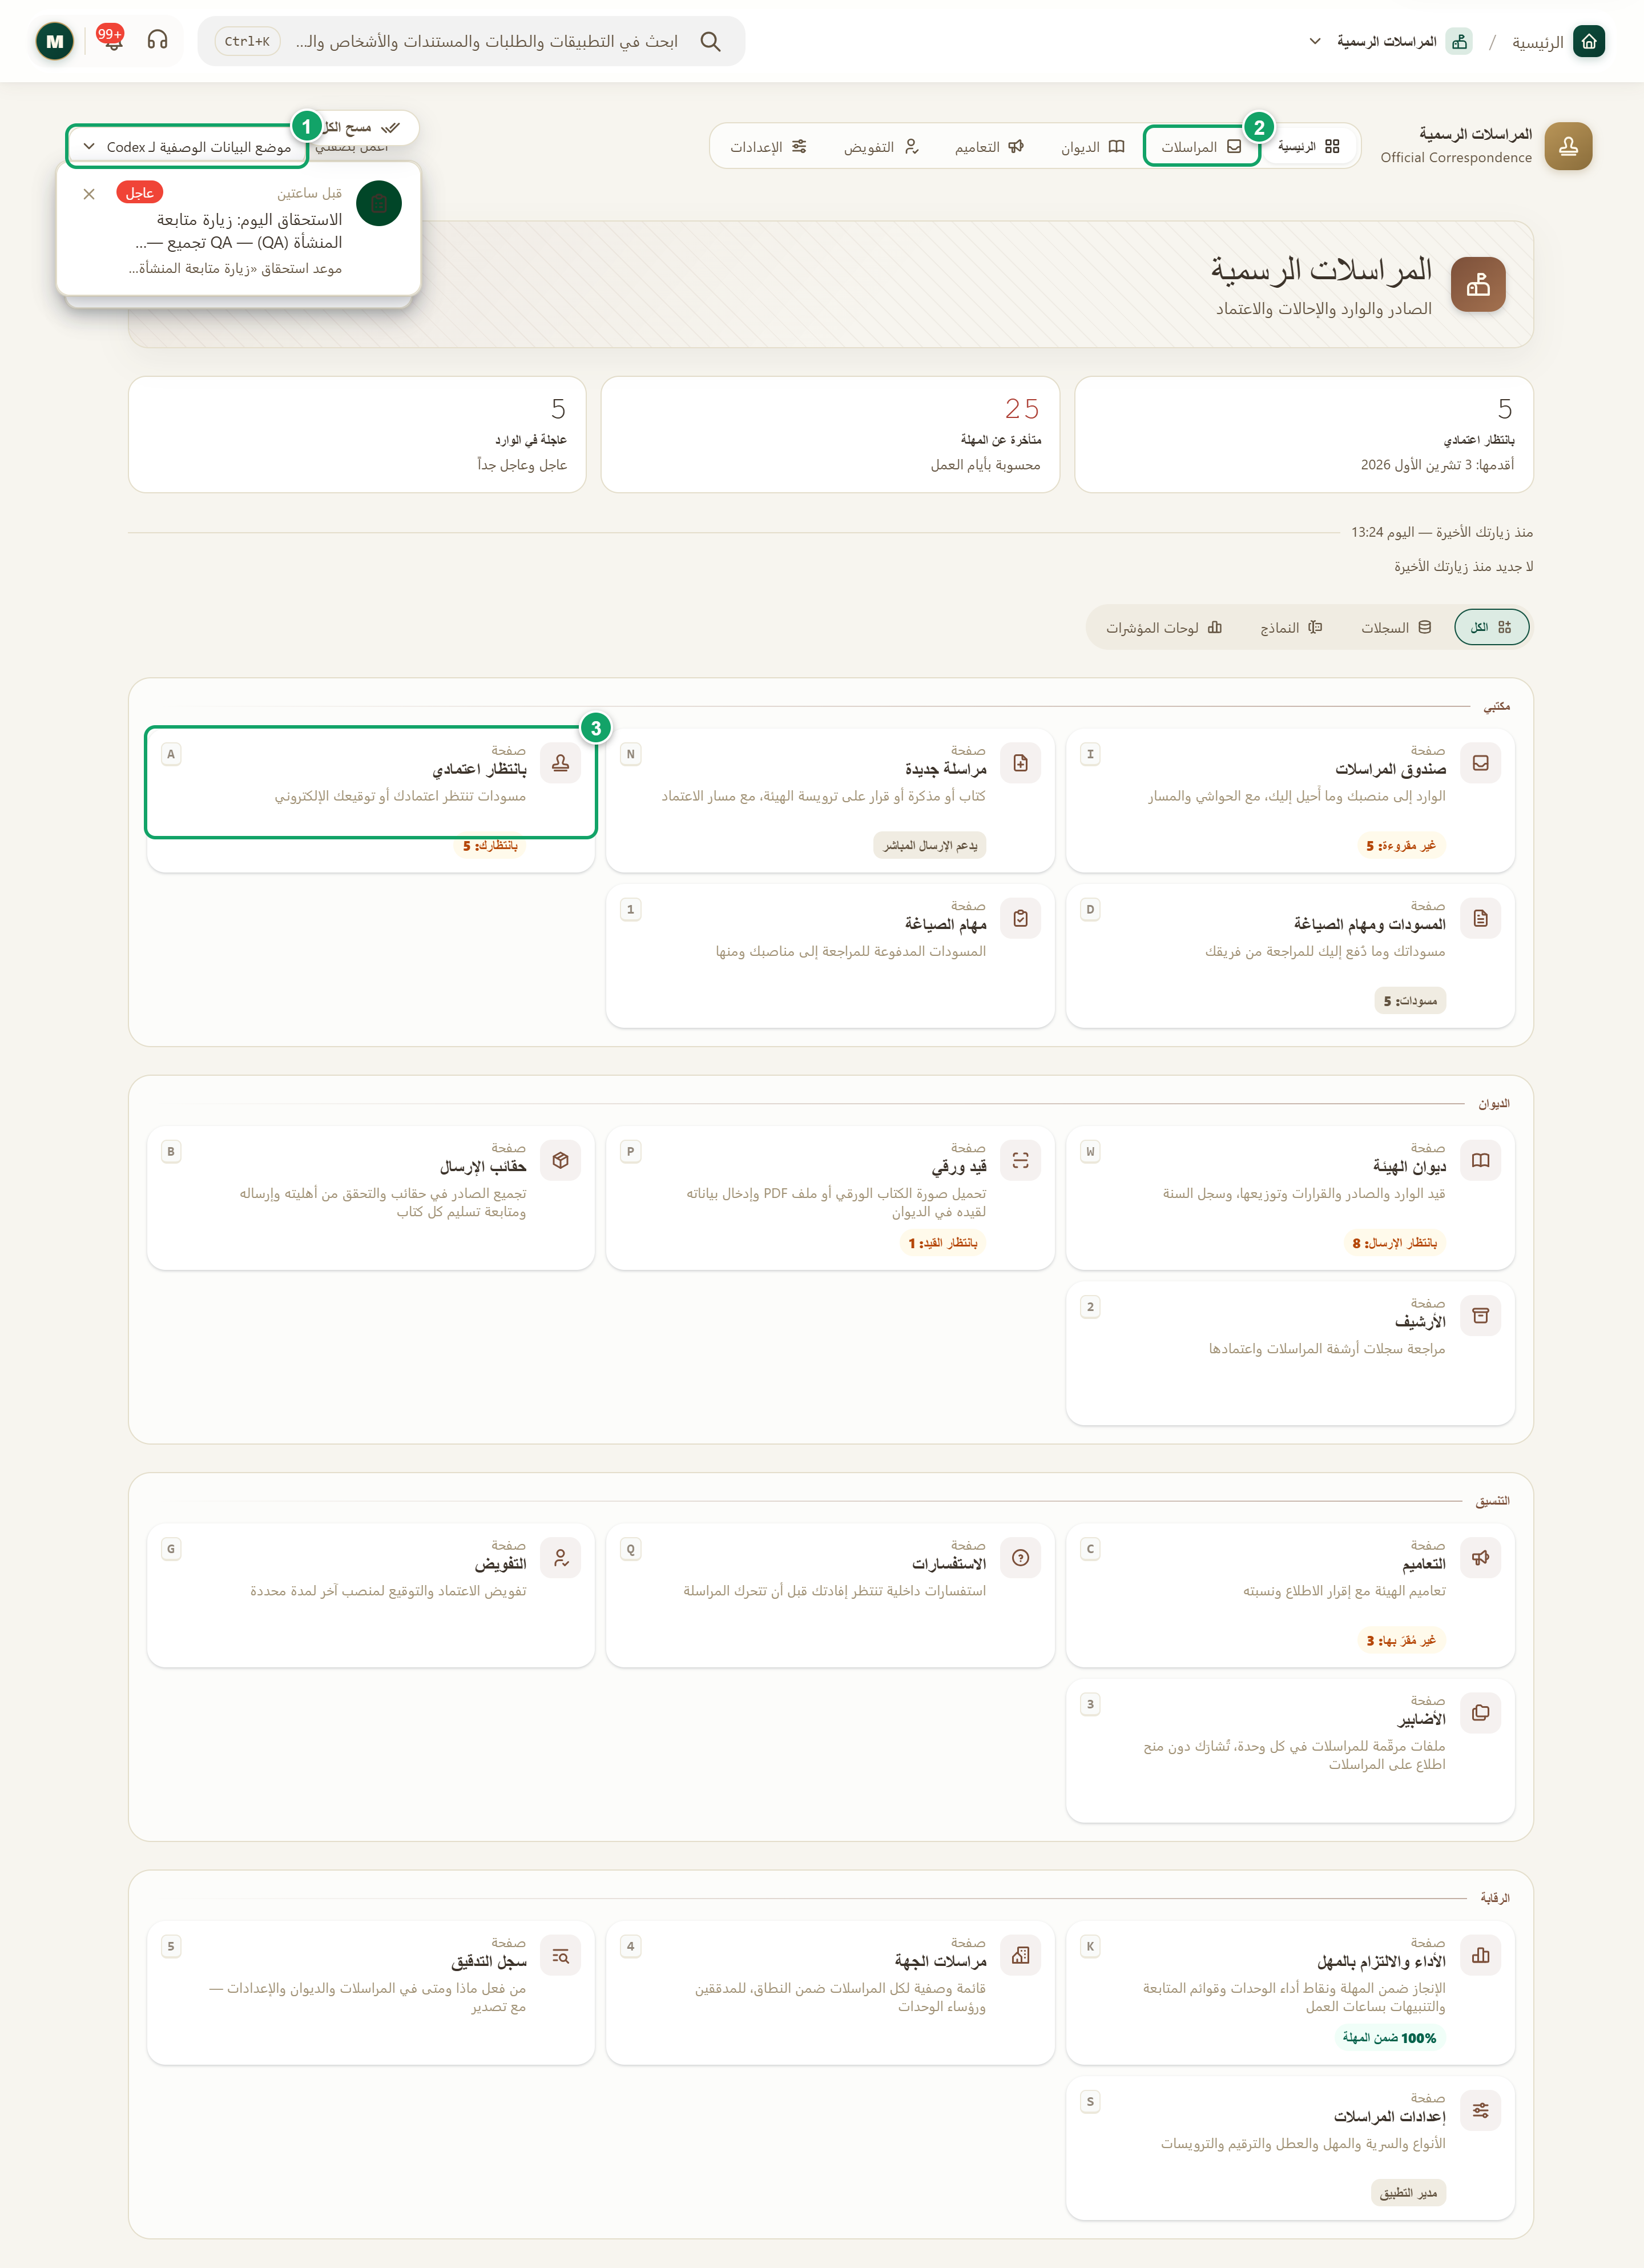
\includegraphics[width=0.95\linewidth,height=0.72\textheight,keepaspectratio]{figures/screens/ch07-home-ar.png}
\caption{الرئيسية ومداخل العمل}
\label{fig:correspondence-home-screen}
\shotnote{تجمع الرئيسية مداخل العمل بحسب المسؤولية، وتعرض أعداداً تساعد على بدء المتابعة. الأرقام تخص سجلات الاختبار ولا تصف مثال الأفق. ① «الصفة» لاختيار المنصب الذي تعمل باسمه. ② «المراسلات» لفتح الصندوق. ③ «بانتظار اعتمادي» لعرض طلبات الاعتماد المتاحة لك.}
\end{figure}


\begin{table}[H]
\centering
\caption{أين تبدأ بحسب عملك؟}
\label{tab:correspondence-responsibilities}
\begin{tabularx}{\linewidth}{R{4.2cm} Y}
\rcHeaderRow
\thh{المسؤولية} & \thh{نقطة البداية}\\
المُعِدّ & ابدأ من «مراسلة جديدة» للإعداد، ومن «المسودات ومهام الصياغة» لاستكمال عمل محفوظ.\\
مراجع الصياغة & افتح «مهام الصياغة» لتعرف المسودات التي دُفعت للمراجعة. المراجعة ليست اعتماداً نهائياً.\\
المعتمد & افتح «بانتظار اعتمادي» وافحص الطلب الموجّه إليك.\\
المستلم & افتح «صندوق المراسلات» ثم «الواردة»؛ أما «نسخ للعلم» فتساعدك على تمييز ما وصلك للاطلاع.\\
موظف الديوان & ابدأ من «ديوان الهيئة» عند توافر صلاحية القيد.\\
مسؤول التهيئة & افتح «إعدادات المراسلات» عند توافر صلاحية الإدارة.\\
\end{tabularx}
\end{table}

\begin{enumerate}
\item افتح تطبيق «المراسلات الرسمية» من مشغّل التطبيقات.
\item اقرأ «أعمل بصفتي»، ثم افتح مدخل العمل الذي يخص مسؤوليتك من الجدول.
\item تحقق من عنوان الصفحة والمجلد؛ فـ«بانتظار اعتمادي» و«المسودات ومهام الصياغة» مدخلان إلى عروض داخل الصندوق.
\end{enumerate}

\textbf{تحقق:} سمِّ مسؤوليتك ونقطة بدايتك قبل متابعة الدليل. إذا غاب الديوان أو الإعدادات، راجع الصلاحية مع المسؤول؛ ولا تستنتج من غياب المدخل أن التطبيق معطّل.

\clearpage
\section{الصفة والصلاحيات}
\label{sec:correspondence-feature-capacity}

الصفة هي المنصب الذي تتعامل مع المراسلات باسمه. قد يرتبط حسابك بأكثر من منصب، وقد يتاح لك منصب آخر بتفويض سارٍ. تغيير الصفة لا يمنحك صلاحية جديدة؛ وتبقى الإجراءات المتاحة مرتبطة بالمراسلة والتعيين والتفويض والصلاحيات.

\begin{rcnote}[مثال: شركة الأفق]
يختار عمر منصبه «منسق عمليات» عند ①، ثم يفتح «المسودات» عند ② ليتابع طلب الزيارة. وإذا فُوّض لاحقاً عن منصب آخر، يميّز العمل نيابةً عنه من عمل منصبه الأصلي.
\end{rcnote}
\begin{figure}[H]
\centering
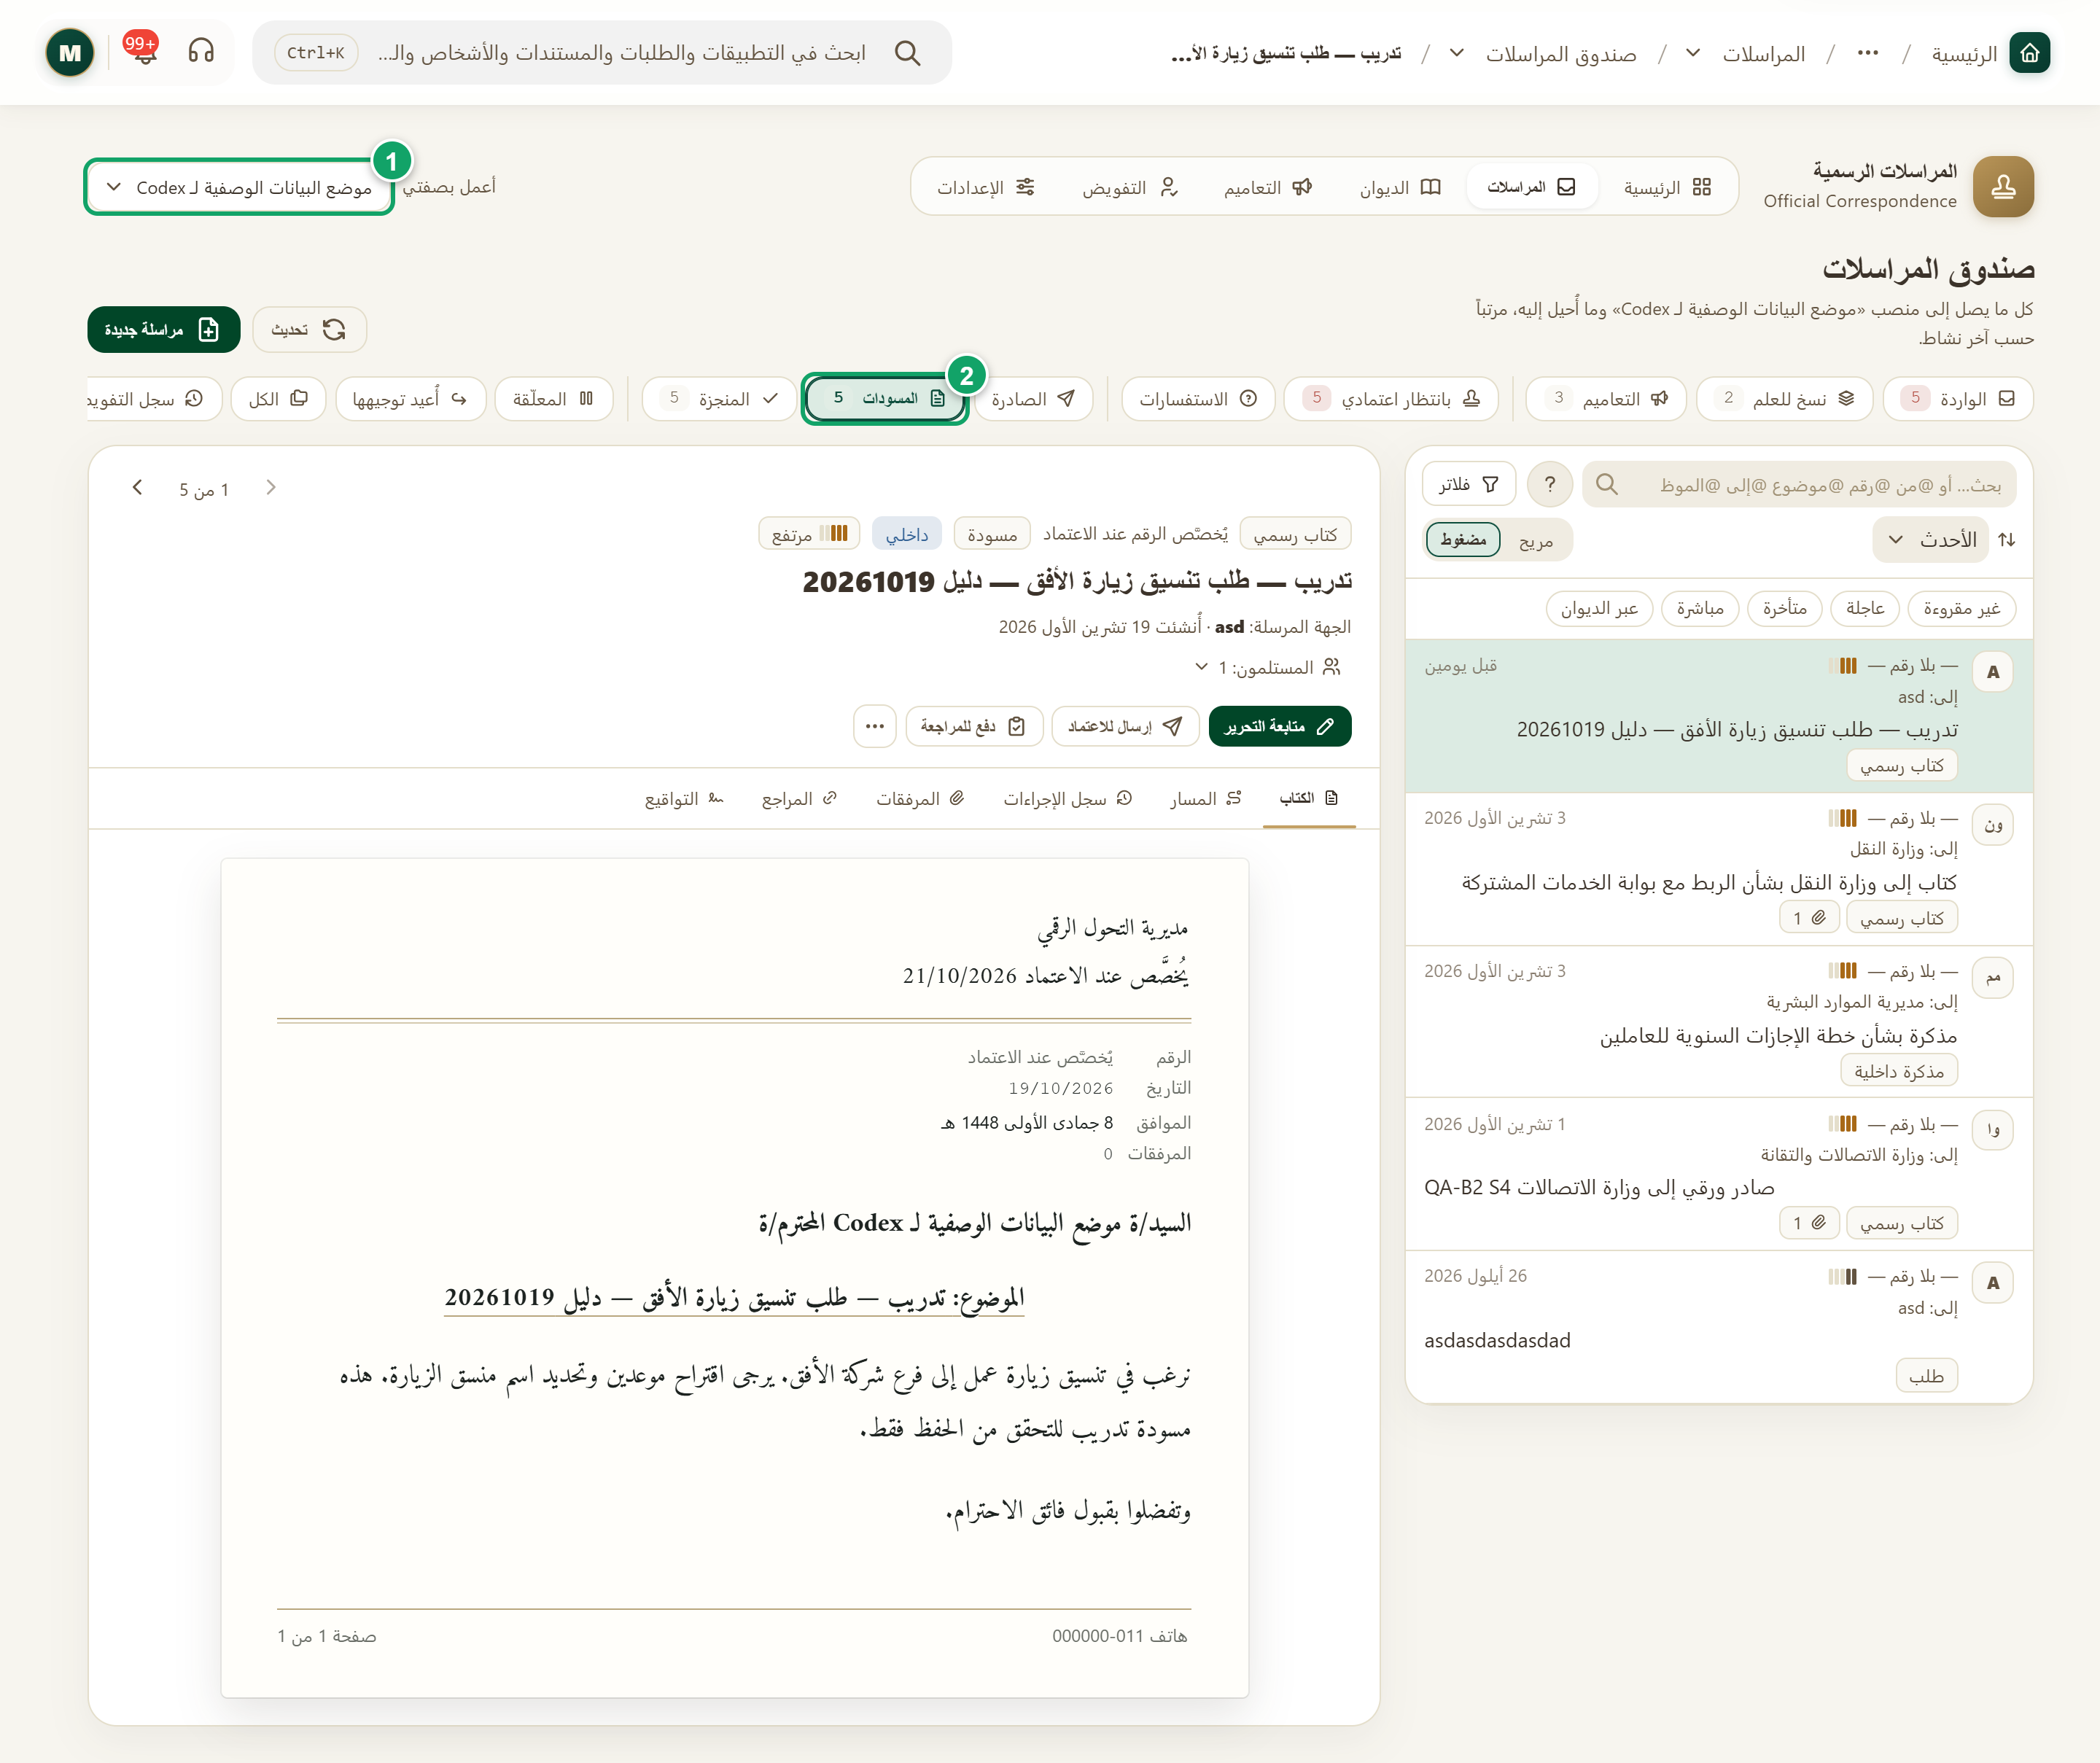
\includegraphics[width=0.95\linewidth,height=0.72\textheight,keepaspectratio]{figures/screens/ch07-capacity-ar.png}
\caption{الصفة ومجلد المسودات}
\label{fig:correspondence-capacity-screen}
\shotnote{تعرض الصورة المنصب المختار وسياق المجلد الذي تتابعه، مع مسودة اختبار مفتوحة. وجود مسودة في الصندوق لا يعني أنها أُرسلت للاعتماد. ① «الصفة» لتحديد المنصب قبل متابعة العمل. ② «المسودات» للعودة إلى الكتب التي ما زالت في الإعداد.}
\end{figure}


\begin{enumerate}
\item افتح «المراسلات الرسمية» وابحث عن «أعمل بصفتي».
\item إذا ظهرت قائمة مناصب، اختر المنصب المطلوب واقرأ اسمه بعد الاختيار. عند إتاحة منصب واحد يظهر الاسم دون قائمة تبديل.
\item عند العمل بالتفويض، افحص عبارة «نيابةً عن» وتاريخ انتهاء التفويض.
\item افتح «صندوق المراسلات» وتحقق من سياق المنصب قبل اختيار مراسلة.
\end{enumerate}

\textbf{تحقق ومعالجة المشكلة:} اذكر المنصب الذي تعمل باسمه، وهل تعمل بالتفويض. إذا غاب المنصب المطلوب، اطلب التحقق من تعيينك أو سريان التفويض وشروطه؛ لا تُنشئ مراسلة باسم منصب آخر لتجاوز المشكلة.

\clearpage
\section{صندوق المراسلات ودورة العمل}
\label{sec:correspondence-feature-tray}

يجمع «صندوق المراسلات» العمل المتاح لك في مجلدات. المجلد وسيلة للعثور على العمل، أما الحالة فتصف مرحلة المراسلة؛ لذلك لا تخلط «بانتظار اعتمادي» مع حالة جميع المراسلات، ولا تعتبر الصدور دليلاً على التسليم أو الإنجاز.

\begin{rcnote}[مثال: شركة الأفق]
تفتح سارة «الواردة» عند ① للعثور على مراسلة تخص زيارة فرع حلب، ثم تبحث عن موضوعها في ②. تستخدم «فلاتر» عند ③ إذا احتاجت إلى تضييق النتائج، وتعيد تحميل القائمة من ④ قبل فحص النتيجة.
\end{rcnote}
\begin{figure}[H]
\centering
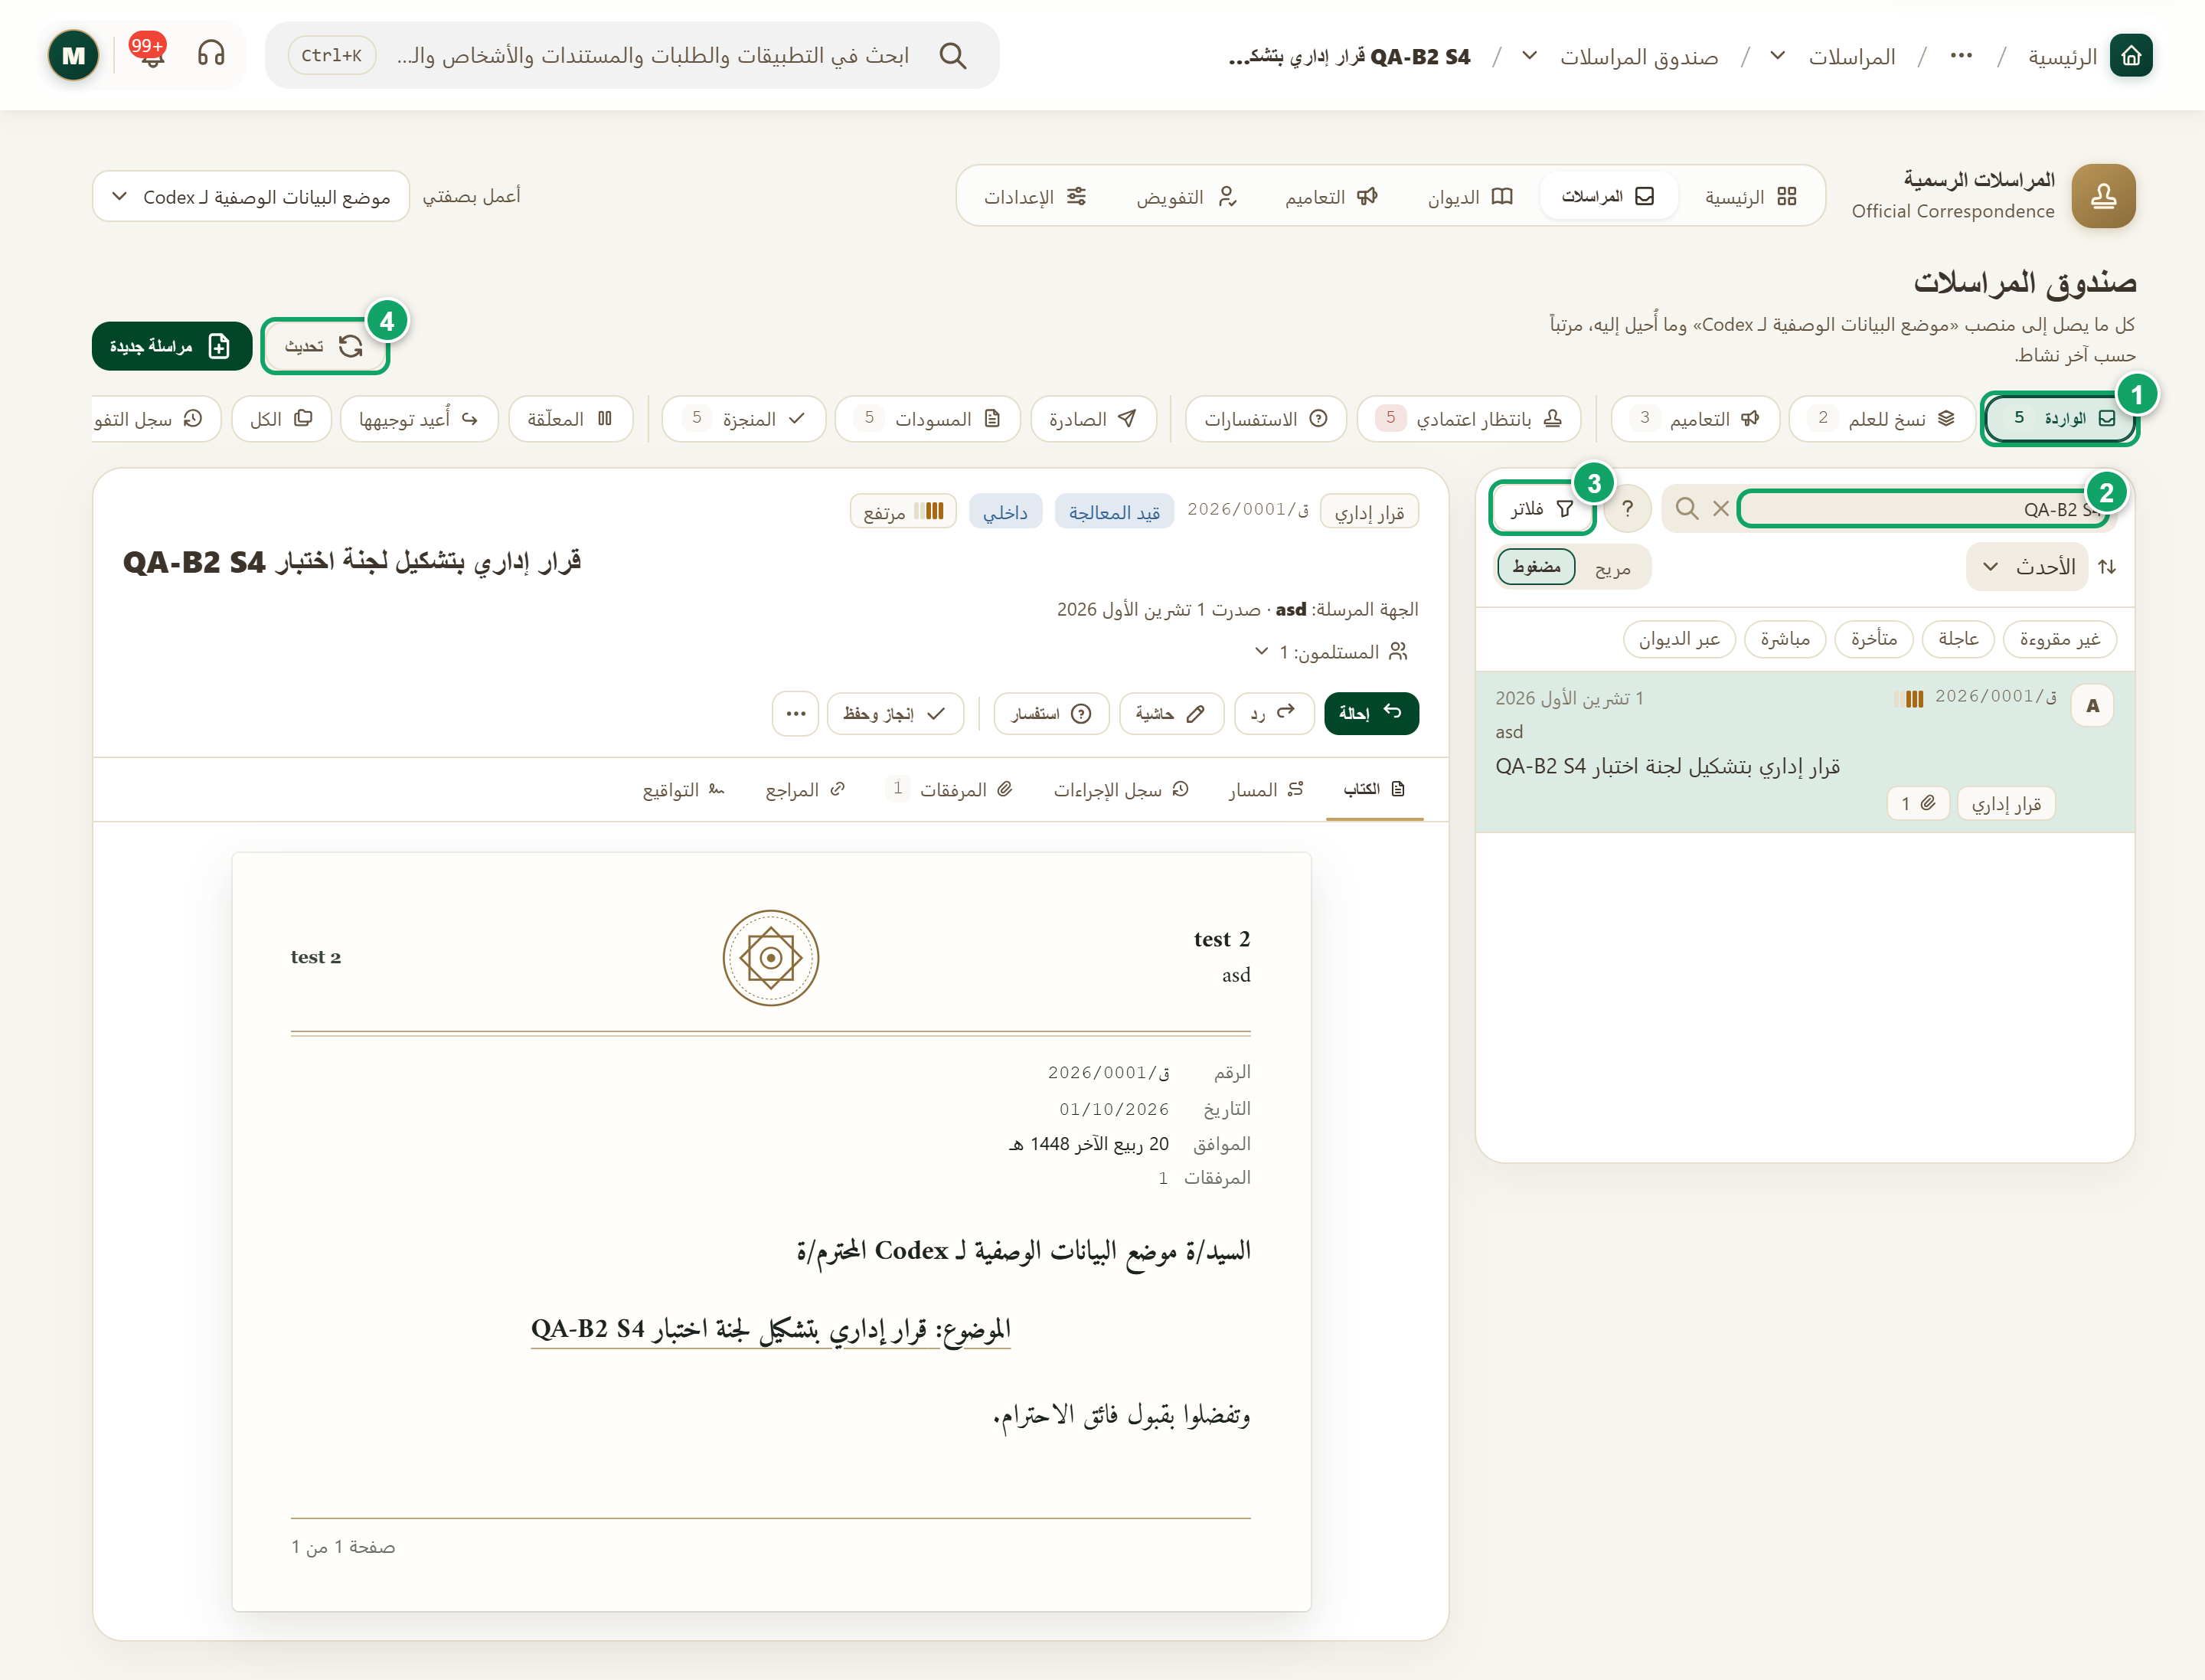
\includegraphics[width=0.95\linewidth,height=0.72\textheight,keepaspectratio]{figures/screens/ch07-tray-ar.png}
\caption{البحث في صندوق المراسلات}
\label{fig:correspondence-tray-screen}
\shotnote{تعرض الصورة نتيجة بحث محدد وكتاب اختبار مفتوحاً، فتستطيع مقارنة الحالة والأولوية والسرية دون الخلط بينها. البحث يضيّق القائمة، ولا يغيّر حالة الكتاب. ① «الواردة» لاختيار المجلد. ② خانة البحث للعثور على موضوع معلوم. ③ «فلاتر» لتضييق النتائج. ④ «تحديث» لإعادة تحميل القائمة.}
\end{figure}


\begin{table}[H]
\centering
\caption{كيف تقرأ بيانات المراسلة؟}
\label{tab:correspondence-reading}
\begin{tabularx}{\linewidth}{R{4.2cm} Y}
\rcHeaderRow
\thh{البيان} & \thh{ما الذي تفهمه منه؟}\\
نوع المراسلة & يحدد تصنيف الكتاب وفق الأنواع التي هيأتها المؤسسة؛ لا تفترض أن قائمة الأنواع موحدة في كل مؤسسة.\\
الحالة & تظهر تسميات مثل «مسودة»، و«بانتظار الاعتماد»، و«أُعيدت للتعديل»، و«صادرة»، و«قيد المعالجة»، و«منجزة»، و«مرفوضة»، و«ملغى». لا تمثل هذه القائمة مساراً إلزامياً واحداً.\\
الأولوية & تساعدك تسميات مثل «عاجل» و«عاجل جداً» على ترتيب المتابعة؛ ولا تعني منح صلاحية إضافية.\\
السرية & تميّز تصنيف الاطلاع، مثل «عام» و«داخلي» و«سري». لا تجعلها مرادفاً للأولوية.\\
المهلة & تساعدك على معرفة ما يستحق المتابعة؛ افحص تاريخ الاستحقاق وما إذا كانت المهلة موقوفة.\\
\end{tabularx}
\end{table}

\begin{enumerate}
\item افتح «صندوق المراسلات»، ثم اختر «الواردة» أو «المسودات» أو «بانتظار اعتمادي» بحسب عملك.
\item اكتب كلمة من موضوع كتاب معلوم في البحث، ثم افحص النتائج. يمكنك استخدام «فلاتر» أو أحد الفلاتر السريعة مثل «غير مقروءة» و«عاجلة».
\item امسح البحث وألغِ الفلتر إذا لم تظهر المراسلة، ثم تحقق من الصفة والمجلد. استخدم «تحديث» لإعادة تحميل القائمة.
\item افتح مراسلة متاحة واقرأ موضوعها وحالتها وأولويتها وسريتها قبل اتخاذ إجراء.
\end{enumerate}

\textbf{تمرين وتحقق:} انتقل من «الواردة» إلى «المسودات» ثم عد، وجرّب بحثاً ثم امسحه. تحقق من تغير المجلد وعودة القائمة؛ وإذا كانت فارغة، سجّل ذلك ولا تعتبره دليلاً على عدم وجود مراسلات في المؤسسة. عند ظهور «تعذّر تحميل المجلد»، استخدم «إعادة المحاولة»؛ فالخطأ ليس نتيجة بحث فارغة.


\end{document}
